\documentclass[10pt]{book}

% Be sure to use PDF Latex
\pdfoutput=1

% links
\usepackage[bookmarks,bookmarksdepth=2, colorlinks=true, linkcolor=blue,citecolor=red, urlcolor=blue]{hyperref}

\usepackage{fullpage}
\usepackage{style-en}


\usepackage[utf8]{inputenc}
% \usepackage[french]{babel}

\graphicspath{{./figures/}}


\newcommand{\myauthor}[3]{#1\protect\footnote{#2, \protect\url{#3}}}


\title{\Huge \sf The Discrete Algebra \\ of the Fourier Transform
\vspace{10mm}
    \begin{center}
    \includegraphics[width=.8\linewidth]{images/natures-mortes-2.JPG}
    \end{center}	 
} 
% \title{\Huge \sf L'algèbre discrète\\de la transformée de Fourier} 


\author{%
\begin{tabular}{c}
	Gabriel Peyr{\'e} \\ CNRS \& DMA \\
	 PSL University, \'Ecole Normale Sup\'erieure \\
	 \url{gabriel.peyre@ens.fr}% \\
%	 \url{https://mathematical-tours.github.io}\\
%	 \url{www.numerical-tours.com}
\end{tabular}
}


\date{\today}

%%

\begin{document}

\maketitle

\chapter*{Forewords}

There are many books on the Fourier transform; however, few are aimed at a multidisciplinary audience. Writing a book for engineers with algebraic concepts is a real challenge, as much, if not more, than writing an algebra book that puts the finger on the applications of the theories encountered. This is the challenge that this book has attempted to meet. Thus, each reader will be able to create a \guill{à la carte} program and draw from statements or computer programs specific elements to establish their knowledge in the field, or apply them to more concrete problems.

The presentation is intentionally very detailed and requires little prior knowledge, mentioned at the beginning of the chapters concerned. 
% There is no doubt that a good student of license should be able to approach this presentation without great difficulty. 
The reader may occasionally need some advanced notions on finite groups as well as some familiarity with group actions. %An aggregative student should be able to find many applications and developments around the official program.
I did not hesitate to repeat the important definitions and notations. For example, the notion of convolution, approached from many angles (abelian group, signal processing, non-commutative group), is each time placed in its context. Thus, the different paragraphs, although following a logical progression, have a real unity and can be read in a non-linear fashion.

The first chapter uses the language of group theory to explain the main concepts and demonstrate the statements that will be used later. The second chapter applies the results obtained to various problems, and constitutes a first contact with fast algorithms (\textit{Walsh transform} for example). The third chapter is an exposition on the discrete Fourier transform. Even if it reinvests the results of the first chapter, it can be read for example by a computer scientist wishing to understand the mechanisms of the algorithms of discrete transforms. The fourth chapter presents various applications of the discrete Fourier transform, and constitutes an essential complement to the previous chapter, to fully understand the mechanisms involved as well as their use in practical situations. The fifth chapter presents more original ideas and algorithms around the Fourier transform, giving rise to numerous applications. The sixth chapter requires some more advanced knowledge, especially some familiarity with finite field theory. It studies valued transforms in a finite field, and presents applications to corrective codes. The last two chapters (the most difficult), are of a more algebraic nature, and propose to generalize the constructions already carried out in the case of finite non-commutative groups. The seventh chapter exposes the theory of linear representations. The eighth and final chapter applies this theory in both theoretical (study of the simplicity of groups) and practical (spectral analysis) fields.

%A good knowledge of the algebraic properties of the Fourier transform is, in my opinion, very useful for constructing aggregation lessons that are both application-oriented and with solid theoretical bases. Many concepts in the aggregation program will be reviewed in this book. First of all, the notion of finite groups is at the heart of the problem approached in this book. Cyclic groups such as $\ZZ / n \ZZ $ are more particularly highlighted: they are the simplest groups, but also the most used in practice. The complex numbers of module 1 are present throughout the talk. The use of Hermitian spaces and unitary transformations is a constant in Fourier theory. The continuous Fourier transform and the Fourier series will be approached only in the exercises, however, the discrete Fourier transform makes it possible to enrich their analysis. Solving partial differential equations makes full use of the algebraic properties of Fourier transforms. Moreover, the calculation of the Fourier coefficients by the fast Fourier transform algorithm, as well as the considerations on the convolution during the resolution by finite differences, make the discrete Fourier transform an essential tool. Finally, the theory of finite fields can also be approached through the world of Fourier.


\index{Matlab} \index{Maple} A number of computer programs are presented; they are written in \textsc{Matlab} for the most part, and in \textsc{Maple} for those which require algebraic manipulations (calculations in finite fields, etc.). Although these are commercial softwares, free software with very similar syntax exists, such as for instance \textsc{Scilab}, \textsc{Octave} and \textsc{Mupad}. 
% 
The choice of a particular language to implement the algorithms is obviously debatable, but the use of \textsc{Matlab} and \textsc{Maple} seems quite natural, these softwares allowing to quickly test the written programs. We can then translate them into a compiled and faster language, such as C or C++. 
%
% In addition, these languages are used for the oral modeling test of the mathematics aggregation. 
%
% The aggregates or future aggregates will therefore not be disoriented. It should be noted that all the programs in this book are available for download, as well as many others, on the \url{https://adtf-livre.github.io/} site.


% I would like to thank my parents, Lucien and Marie-No\"{e}lle, who supported me throughout the writing of this book. Finally, I address my deepest gratitude to my proofreaders, who provided their experience to point me in the right direction: Abdellah Bechata, Vincent Beck, Christophe Bertault, Jérôme Malick and Jean Starynkévitch.

% \vskip 3mm \begin{minipage}[c]{.8\linewidth} \end{minipage}\hfill \begin{minipage}[c]{.2\linewidth} Gabriel Peyré. \end{minipage}\newpage 
%  \thispagestyle{empty} 

\tableofcontents 


\chapter{Fourier transform on a finite group}
\label{chap-transforme-fourier-finite-group}



In this first chapter, we will approach the study of the Fourier transform from an original angle, that of group theory. Fourier theory, whether viewed from an algebraic point of view or not, consists above all in the analysis of functions. Here we must take the word analysis literally, in its etymological sense. It's about breaking down complex data into a simpler form. It will therefore be a question of constructing a systematic means to obtain this decomposition, and this is precisely where the Fourier tools come into play. To achieve this decomposition efficiently, we must still use a certain amount of a priori information about the functions we are studying. This first chapter will relate to the study of functions on a finite group; the \guill{elementary bricks} decomposition carried out by the Fourier analysis will result from the symmetries inherent in the group structure. \index{Symmetry}

The most elementary framework to carry out this project is that of finite commutative groups, since one does not have to worry about either the regularity of the functions encountered, or the convergence of the manipulated series (since they are finite!). Of course, one will be tempted to cry scandal as the work then accomplished seems simplistic compared to the \guill{analytic} theory of Fourier series. However, this study makes it possible to bring new points of view and to pose new questions which will be addressed in the next chapters.
\begin{rs}
\item How can the study of the Fourier transform on a finite group help us to understand the construction of the continuous Fourier transform?
\item How does the Fourier transform on finite groups join the discrete Fourier transform?
\item What uses can we make of the Fourier transform on a finite group? How to build efficient algorithms, and how to implement them?
\item Finally, what happens to this theory when we try to apply it to non-commutative groups? This question will motivate the introduction of new tools, described in detail in the last two chapters.
\end{rs} It is to this set of questions that we will try to answer. The methods implemented are multiple, they often borrow from several mathematical disciplines.

There are many references to the subject of duality on finite groups. There is of course the book of \nompropre{J.P.Serre} \cite{serre}, but also for example that of \nompropre{Warusfel} \cite{warusfel}, for a more detailed presentation. For an introduction to the Fourier transform on a commutative group, we can look at the work of \nompropre{Dym} and \nompropre{Mac Kean} \cite{dym}.

% ------------------------------------------------- -----
% ------------------------------------------------- -----
% ------------------------------------------------- -----
% section - Dual of a finite group
% ------------------------------------------------- -----
% ------------------------------------------------- -----
% ------------------------------------------------- -----
\section{Dual of a finite group}
% \addcontentsline{toc}{section}{Dual of a finite group}
\label{sect1-dual-group}

The aim of this book is to study, from an algebraic point of view, the functions with complex values whose starting space is a finite group denoted by $G$. It is a question of making maximum use of the properties of the group to obtain interesting functional decompositions. The basic idea of this chapter, the one which will guide our reflections until the end of this book, consists in studying how we can represent a function on a group $G$. The generally most common way to think about a function $ f: G \rightarrow \CC$ is to consider the set of its values $ f(g)$ for $ g \in G$. The major disadvantage of this representation is that it does not exploit the structure of our group $G$ at all. In a way, it is a universal representation, which does not depend at all on the group that one has chosen. To study a function efficiently, it seems logical to build a new representation that exploits the symmetries that can be found in a group $G$. The simplest example of these symmetries is the cyclic character of the group $\ZZ/n\ZZ$, but we can of course consider more complex constructions.

% ------------------------------------------------- -----
% ------------------------------------------------- -----
% sub-section - Definitions
% ------------------------------------------------- -----
% ------------------------------------------------- -----
\subsection{Definitions}

\index{Subgroup} To understand how a function can be more or less simple to represent, we will first approach the simplest functions, those which do not oppose any resistance to the structure of the starting group $G$. We are therefore going to focus on the functions that carry the structure of the group. These functions are the morphisms of the group $G$ into a group of the arrival set, that is, a subgroup of $\CC^*$. We will therefore introduce the appropriate definitions.

\begin{defn}[Characters and dual of a group]
\label{notation-0} \label{notation-1} \index{Dual!of a finite abelian group} \index{Character!of an abelian group} \index{Duality!on a group} Let $G$ a finite group. By definition, a \textit{character}$\chi$ is a morphism from the group $G$ into the multiplicative group $\CC^*$. We denote by $\wh{G}$ the set of characters, which we call the \textit{dual} of $G$.
\end{defn}
$\wh{G}$ is a group for multiplication of applications. It is recalled that this multiplication is defined as follows.
\begin{equation*}
\forall(\chi_1, \, \chi_2) \in \wh{G}^2, \quad \chi_1 \chi_2: x \mapsto \chi_1 (x) \chi_2 (x).
\end{equation*}
We will see, in particular in Paragraph~\ref{sect2-bidual}, that the duality over a finite group has many points in common with the duality between vector spaces. In the next chapter, more precisely in Paragraph~\ref{abelian-finite-grpe-fish-formula}, we will even see that in certain cases, this rapprochement can become an identity between the two structures (of group and of vector space). The duality on a finite group then makes it possible to demonstrate interesting linear properties. In the meantime, let's start by studying the image of a character $\chi \in \wh{G}$.

\begin{prop}
\label{prop-pte-elem-car}
\index{Morphism!character} \label{notation-2} \label{notation-3} \label{notation-4} \label{notation-5} Let $G$ be a finite group of cardinal $|G| = n $. The elements of $\wh{G}$ are in fact the morphisms of $G$ in the group of the \ordin{n}{ith} roots of the unit,
\begin{equation*}
\UU_n = \left\{\exp \left(\frac{2 \imath k \pi}{n} \right) \; \bigg \backslash \; 0 \leq k <n \right\}.
\end{equation*}
In particular,
\begin{equation*}
\forall g \in G, \quad |\chi(g) | = 1, \quad \chi(g^{-1}) = \chi(g)^{-1} = \ol{\chi(g)},
\end{equation*}
where we denote by $|z|$ the modulus of a complex number $ z $, and $\ol{z}$ its conjugate.
\end{prop}

\begin{proof}
\index{Root!of unit} Denote by $ 1$ the neutral element of $G$. Note that for any element $ g \in G$, we have $ g^n = 1$. This therefore implies, for all $\chi \in \wh{G}$, that $\chi(g)^n = \chi(g^n) = 1$, which means that $\chi$ is at values in the set of \ordin{n}{th} roots of the unit.
\end{proof}


\begin{rem}
It follows that in particular, $\wh{G}$ is a finite group (because there is only a finite number of maps of $G$ in $\UU_n$, which are finite sets) , commutative. Moreover, every element $\chi \in \wh{G}$ is constant over the conjugation classes of $G$, since
\begin{equation}
\label{eq-character-constant-class-conjug}
\forall (g, \, h) \in G^2, \quad \chi(h^{-1} gh) = \chi(h)^{-1} \chi(g) \chi(h) = \chi(e) \chi(g) = \chi(g).
\end{equation}
\end{rem}


\begin{defn}[Function space on $\mbold{G}$]
\label{defn-space-function-g-in-c}
\index{Space!of functions of $G$ in $\CC$} \label{notation-6} \label{notation-7} We denote by $\CC[G]$ the set of functions of $G$ in $\CC$. The notation $\CC[G]$ will be explained in Paragraph~\ref{sect2-algebre-grpe-abelien}. It is a vector space on $\CC$. We define a Hermitian dot product, by \label{notation-8} \label{notation-9} \label{notation-10}
\begin{equation}
\label{eq-defn-prod-herm-c-g-abelien}
\forall (f, \, g) \in \CC[G]^2, \quad \dotp{f}{g} \eqdef \frac{1}{|G|} \sum_{x \in G}{f (x) \ol{g (x)}}.
\end{equation}
We also define a norm $\norm{\cdot}_2 $ on $\CC[G]$ by $\norm{f}_2^2 \eqdef \dotp{f}{f}$.
\end{defn}


\begin{rem}
\label{notation-11} \index{Translation} The Hermitian product that we have just defined on $\CC[G]$ presents strong similarities with the one that can be defined between two functions of $L^2(\RR)$ as follows:
\begin{equation*}
\forall (f, \, g) \in L^2(\RR)^2, \quad \dotp{f}{g} = \int_{\RR}{f (x) \ol{g (x)} \d x}.
\end{equation*}
The main difference is the change of the sum to integral. One of the common properties of these two dot products is translational invariance. Indeed, if we denote by $ T_y (f)$ the function $ x \in G \mapsto f (xy) \in G$ (or its continuous analogue $ T_y (f) = f(\cdot + y)$), we have
\begin{equation*}
\dotp{T_h (f)}{T_h(g)} = \dotp{f}{g}.
\end{equation*}
This property will be constantly used thereafter, among other things to demonstrate the orthogonal relations between characters.
\end{rem}
In order to study the functions of $\CC[G]$, we will introduce a canonical basis. The decomposition in this base corresponds to the standard way of representing a function of a set in $\CC$.

\begin{prop}
\label{prop-base-c-g}
\index{Base!of $\CC[G]$} A basis of $\CC[G]$ is given by the following $(\delta_g)_{g \in G}$ functions:
\begin{equation}
\label{eq-defn-delta-function-g}
\delta_g(h) \eqdef \left\{\begin{array}{lll} 1 & \text{if} & h = g \\0 & \text{if} & h \neq g \end{array} \right. .
\end{equation}
In particular, $\CC[G]$ is a vector space of dimension $n = |G|$ on $\CC$.
\end{prop}
\begin{proof}
We immediately check that the family is orthonormal for the Hermitian product \eqref{eq-defn-prod-herm-c-g-abelien}. As these functions are not zero, this implies that they form a free family of $\CC[G]$. The fact that this family is also a generator comes from the canonical decomposition
\begin{equation}
\label{eq-decomposition-c-g-dirac-abelien}
\forall f \in \CC[G], \quad f = \sum_{g \in G}{f(g) \delta_g},
\end{equation}
which ends the demonstration.
\end{proof}
This proposition allows to immerse $G$ in $\CC[G]$ in a canonical way by $ g \mapsto \delta_G$. Moreover, we have seen that any function $ f \in \CC[G]$ decomposes in the base $\{\delta_g\}_{g \in G}$, this is what the equation expresses \eqref{eq-decomposition-c-g-dirac-abelien}. This decomposition is apparently very simple. We will however see in Paragraph~\ref{sect2-convolution-transforme-fourier}, with the notion of \textit{convolution}, that it does not facilitate calculations at all. This is why we are going to look for a database which has the following two properties. 
\begin{rs}
\item It must be easy to use (the decomposition in this base must be easy to calculate).
\item It must have interesting properties for the algebraic operations that we want to use (linear combination, product, and product of convolution of functions).
\end{rs} 
The character family, formed from the elements of $\wh{G}$, might be a good candidate; it remains to be shown that she possesses the required qualities.

% ------------------------------------------------- -----
% ------------------------------------------------- -----
% sub-section - Dual of a cyclic group
% ------------------------------------------------- -----
% ------------------------------------------------- -----
\subsection{Dual of a cyclic group}
\label{sect1-dual-cyclic-group}


Before launching into the general study of duality on any group, let's take the time to see how all this behaves in the simplest case, that of a cyclic group (whose archetype is $\ZZ/n\ZZ$, for a given integer $n$). In fact, this example is of prime importance, on the one hand because in practice, it is the structure that we meet most often (we will see in chapter \oldref{chap-tfd} that unidimensional calculations in signal processing use the structure of $\ZZ/n\ZZ$), and secondly because we will use these results to demonstrate the general case.

\begin{prop}[The cyclic case]
\label{prop-cyclic-case}
\index{Group!cyclic} Let $ G = \{1, \, g_0, \, g_0^2, \ldots, \, g_0^{n-1}\}$ be a cyclic group of cardinal $n$ and generator $ g_0 $. \label{notation-12} Let $\omega $ be a primitive root \ordin{n}{th} of the unit, for example $\omega = e^{\frac{2 \imath \pi}{n}}$. The elements of $\wh{G}$ are of the form, for $ j \in \{0, \ldots, \, n-1\}$,
\begin{equation*}
\chi_j: \func{G}{\CC^*}{g = g_0^k}{(\omega^j)^k = e^{\frac{2 \imath \pi j k}{n}}}.
\end{equation*}
\label{notation-13} In particular, we have $ G \simeq \wh{G}$.
\end{prop}
\begin{proof}
To determine a character $\chi \in \wh{G}$, we need to calculate the value of $\chi(g_0^k)$, for $ k \in \{0, \ldots, \, n-1\}$, which gives
\begin{equation*}
\chi(g_0^k) =(\omega^j)^k = \omega^{j k}.
\end{equation*}
In this equality, we have noted $\omega^j \eqdef \chi(g_0)$, with $0 \leq j \leq n-1$, since, as we have seen in the proposition \ref{prop-pte-elem-car}, this quantity is a \ordin{n}{th} root of the unit. So our character $\chi \in \wh{G}$ is indeed one of $\{\chi_0, \ldots, \, \chi_{n-1}\}$. Conversely, we see that, for $ j \in \{0, \ldots, \, n-1\}$, the maps $\chi_j $ are indeed morphisms from $G$ into $\CC^*$, so are indeed elements of $\wh{G}$. \\Finally, if we identify the elements of $\ZZ/n\ZZ$ and their representatives in $\{0, \ldots, \, n-1\}$, we define an application $\psi: j \mapsto \chi_j $ from $\ZZ/n\ZZ$ in $\wh{G}$. We saw that this application was surjective. On the other hand, this application is injective (it suffices to evaluate $\chi_j = \psi (j)$ in $ g_0 $) and it is a morphism (elementary verification). It is therefore an isomorphism and therefore $\wh{G}$ is isomorphic to $\ZZ/n\ZZ$, itself isomorphic to $G$.
\end{proof}
The figure \figref{fig-cyclic-characters} shows the first four characters of the group $\ZZ/12 \ZZ$. On the x-axis, we have denoted $\{0, \ldots, \, 11\}$ the representatives of the group $\ZZ/12 \ZZ$, and the character values are denoted $ *$. The top line shows the real parts of the characters, and the bottom line the imaginary parts. We can see that the points are regularly spaced along the curves of equations $ y = \cos \left(\frac{2 \pi}{N} x \right)$ and $ y = \sin \left(\frac{2 \pi}{N} x \right)$.

\begin{figure}[ht]
    \begin{center}
    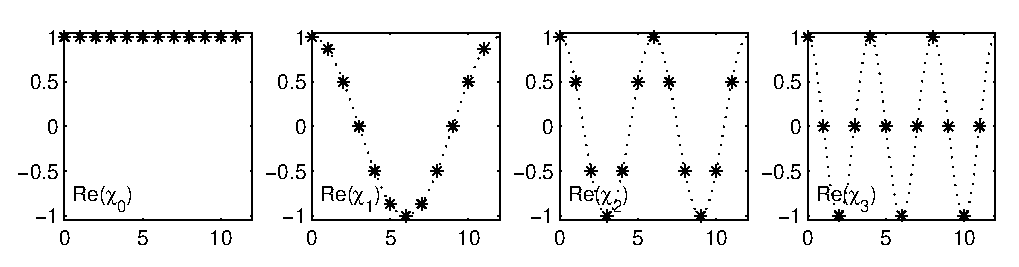
\includegraphics[scale=.7]{images/caracteres-cycliques-1.eps}
    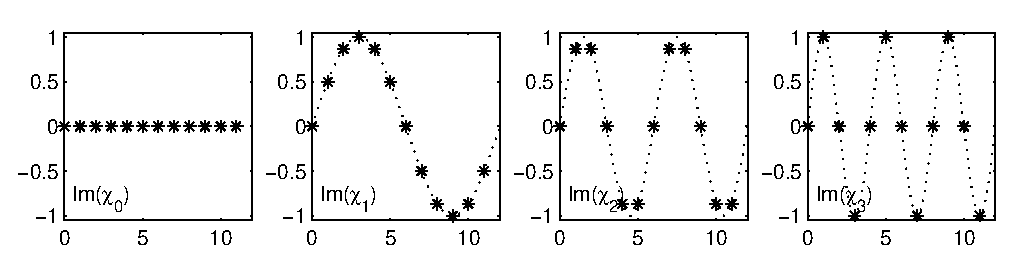
\includegraphics[scale=.7]{images/caracteres-cycliques-2.eps}
    \end{center}
    \caption{The first four characters of the group $\ZZ/12\ZZ$}
\label{fig-cyclic-characters}
\end{figure}


\begin{rem}
We can already notice that this isomorphism is not canonical, since it depends on the choice of the primitive root of the unit $\omega $ chosen. This phenomenon is recurrent in the study of duality (we find it in the linear duality between vector spaces), the dual not being canonically isomorphic to the starting group. All this will be specified later, in particular in Paragraph~\ref{sect2-bidual}.
\end{rem}


\begin{rem}
\label{rmk-zpz-isomorphism}
\index{Isomorphism!between $G$ and $\wh{G}$} Any cyclic group is isomorphic to $\ZZ/n\ZZ$ for $n = |G|$. In a way, the study of the duality on the group $\ZZ/n\ZZ$ sums up the one that we can do on any other cyclic group. In the remainder of the presentation, we will consider groups built from the elementary bricks that are groups of the type $\ZZ/n\ZZ$. This is why we must keep in mind the structure of duality on these particularly simple groups. By applying the proposition \ref{prop-cyclic-case}, we obtain the isomorphism that must be retained:
\begin{equation*}
\forall n \in \NN^*, \quad \wh{\ZZ/n\ZZ} \simeq \ZZ/n\ZZ.
\end{equation*}
We will see that in fact this property extends to any finite commutative groups.
\end{rem}


Before closing this paragraph, notice that we have $|\wh{G}| = |G| = \dim_{\CC}(\CC[G])$. We even have a stronger property.

\begin{prop}
\label{prop-base-ortho-cyclic-case}
\index{Base!orthogonal} Let $G$ be a cyclic group. $\wh{G}$ forms an orthonormal basis of $\CC[G]$, which means that
\begin{equation*}
\forall (p, \, q) \in \{0, \ldots, \, n-1\}^2, \quad \dotp{\chi_p}{\chi_q} = \delta_p^q,
\end{equation*}
where we define the symbol of \textit{Kroneker}$\delta_p^q $ as follows:
\begin{equation*}
\delta_p^q = \left\{\begin{array}{ccc} 0 & \text{if} & p \neq q \\1 & \text{if} & p = q \end{array} \right. .
\end{equation*}
\index{Kroneker's!symbol} \label{notation-14}
\end{prop}

\begin{proof}
We can assume that $ G = \ZZ/n\ZZ$. \\We write $\wh{G} = \{\chi_i\}_{i = 0}^{n-1}$, with $\chi_i (k) = \omega^{ik}$, where $\omega $ is a primitive \ordin{n}{ième} root (according to the proposition \ref{prop-cyclic-case}). We then have
\begin{equation}
\label{eq-orthogonalite-cyclic-case}
\forall (p, \, q) \in \{0, \ldots, \, n-1\}^2, \quad \dotp{\chi_p}{\chi_q} = \frac{1}{n} \sum_{i = 0}^{n-1}{(\omega^{pq})^{i}} = \delta_p^q
\end{equation}
(we obtain the last equality by summing the geometric series of reason $\omega^{p-q}$). \\The family $\wh{G} = \{\chi_i\}_{i = 0}^{n-1}$ is therefore orthonormal, and therefore in particular free. To conclude that it does indeed form a base, it suffices to notice that its cardinality is equal to the dimension of $\CC[G]$, since we have seen that $|G| = |\wh{G}|$.
\end{proof}


\begin{rem}
The proof of the orthogonality of the characters in the general case of an abelian group is hardly more complicated, and will be exposed to the proposition \ref{prop-orthogonalite-car-grpe-abelien}. However, the proof that we have just made is essential since it is at the base of the results of the one-dimensional Fourier transform, which will be presented in the Section~\ref{sect1-language-processing-signal}.
\end{rem}

% ------------------------------------------------- -----
% ------------------------------------------------- -----
% ------------------------------------------------- -----
% section - Dual of an abelian group
% ------------------------------------------------- -----
% ------------------------------------------------- -----
% ------------------------------------------------- -----
\section{Dual of an abelian group}
% \addcontentsline{toc}{section}{Dual of an abelian group}
\label{sect1-dual-abelien-group}

Our goal is to extend the result we have just demonstrated ($\wh{G}$ is an orthonormal basis of $\CC[G]$) to any finite abelian group. To achieve this, we will use a purely algebraic approach, which uses a character extension theorem. Then, we will establish a stronger result, namely that we have in fact an isomorphism between $\wh{G}$ and $G$, property that once again we have proved in the case of cyclic groups .
% ------------------------------------------------- -----
% ------------------------------------------------- -----
% sub-section - Algebraic approach
% ------------------------------------------------- -----
% ------------------------------------------------- -----
\subsection{Algebraic approach}
\label{sec2-approach-algebraic-dual-abelien}

The following lemma is the main result in the study of the structure of $\wh{G}$.

\begin{lem}[character extension]
\label{lem-prolongation-caractere}
\index{Character extension} \index{Subgroup} Let $G$ be a commutative finite group and $ H \subset G$ a subgroup. Any $\chi$ character of $H$ can be extended into a $G$ character.
\end{lem}
\begin{proof}
\label{notation-15} We perform a recurrence on $[G:H] = | G/H |$ the index of $H$ in $G$. The property being trivial for $[G:H] = 1$, since $ G = H $; we therefore assume $[G:H]> 1$, which allows us to take $ x \in G$ such that $ x \notin H $. Let $ K = \langle H, \, x \rangle $ be the group generated by $ x $ and $H$. Let $n$ be the smallest integer such that $ x^n \in H $. Any element $ z \in K $ is written uniquely as $ z = yx^k $ with $ y \in H $ and $ k \in \{0, \ldots, \, n-1\}$. Indeed, if $ yx^k = y'x^{k'}$, with $0 \leq k \leq k'\leq n-1$, then we have $ x^{k-k'} \in H $ and $ kk'<n $, therefore necessarily $ kk' = 0 $ by definition of $n$. \\\textbf{Analysis:} Suppose we have an extension $\wt{\chi}$ of $\chi$. \\Let $\zeta = \chi(x)$. We need $\zeta^n = \chi(x^n) = \chi(1) = $ 1. So $\zeta$ must be a \ordin{n}{th} root of the unit. We then have, necessarily, if $ z \in K $ is written $ z = y x^k $ with $ y \in H $ and $0 \le k \le n-1$,
\begin{equation}
\label{eq-formula-extension-character}
\wt{\chi} (z) = \wt{\chi} (y x^k) = \chi(y) \zeta^k.
\end{equation}
\textbf{Summary:} let $\zeta$ be a \ordin{n}{th} root of the unit. Let us define, for $ z \in K $ decomposed as previously in the form $ z = y x^k $, the extension $\wt{\chi}$ by the equation \eqref{eq-formula-extension-character}. This is to show that \eqref{eq-formula-extension-character} does indeed define an element of $\wh{K}$. The uniqueness of the decomposition shows that the definition is not ambiguous. To show that it is indeed a morphism, it suffices to take $ h = yx^k $ and $ h'= y' x^{k'}$ two elements of $ K $, and to distinguish two cases. \begin{rs}
\item If $0 \leq k + k'\leq n-1$, then we have \\$\displaystyle{\wt{\chi} (h h') = \wt{\chi} (yy'x^{k + k'}) = \chi(y y') \zeta^{k + k'} = \chi(y) x^k \chi(y') x^{k'} = \wt{\chi}(h) \wt{\chi} (h')}$.
\item If $n \leq k + k'\leq 2n-1$, we can come back to the previous case, \\$\displaystyle{\wt{\chi} (h h') = \wt{\chi} (yy'x^nx^{k + k' - n}) = \chi(y) \chi(y') \chi(x^n) \zeta^{k + k' - n} = \wt{\chi}(h) \wt{\chi} (h')}$.
\end{rs} The multiplicativity property of degrees tells us that
\begin{equation*}
	[G:H] = [G:K] [K:H], \quad \text{with} \quad [K:H]> 1.
\end{equation*}
So we have $[G:K] <[G:H]$. We can with the induction hypothesis extend $\wt{\chi}$ to $G$.
\end{proof}
As the (arbitrary) choice of the root \ordin{n}{th} of the unit $\zeta$ shows, the character extension is of course not unique. However, it is this result which will allow us to demonstrate that $G$ and $\wh{G}$ have the same cardinality. To do this, let's start by translating the result of character extension in terms of a quotient group.

\begin{lem}
\label{lem-suite-exact}
\index{Sequence!exact} \index{Morphism!of restriction} \index{Morphism!of extension} We denote by $\rho: \wh{G} \twoheadrightarrow \wh{H}$ the restriction morphism and $ j : \wh{G/H} \hookrightarrow \wh{G}$ the extension morphism, defined by
\begin{equation*}
j: \func{\wh{G/H}}{\wh{G}}{\chi}{\wt{\chi}} \quad \quad \text{with} \quad \wt{\chi} ( x) \eqdef \chi(x H).
\end{equation*}
We have the exact sequence:
\begin{equation*}
\{1\} \rightarrow \wh{G/H} \overset{j}{\hookrightarrow} \wh{G} \overset{\rho}{\twoheadrightarrow} \wh{H} \rightarrow \{1\} .
\end{equation*}
\end{lem}
\begin{proof}
By the lemma \ref{lem-prolongation-caractere}, $\rho$ is surjective. \\Moreover, if we consider $\chi \in \Ker(\rho)$, then $ H \subset \Ker(\chi)$, and therefore by the universal property of the quotient, there exists a unique $\wt{\chi} \in \wh{G/H}$ such that $\chi(x) = \wt{\chi} (x H)$, i.e. $ j(\wt{\chi}) = \chi$. \\Conversely, an element of $\Im(j)$ is trivial over $H$, which shows that we have $\Ker(\rho) = \Im(j) = \wh{G/H}$.
\end{proof}


\begin{cor}
\label{cor-order-dual-equal-order-group}
\index{Group!order of a group} Let $G$ be a finite commutative group. Then $\wh{G}$ is of the same order as $G$.
\end{cor}
\begin{proof}
We reason by induction on $n = |G|$. For $n = 1$, the result is trivial because $\wh{G} = \{1\}$, where we denote 1 the trivial character on $G$ (i.e. the function which has any element associatinG$ 1$). Let therefore $n \geq 2 $, which allows to consider a non-trivial cyclic group $ H \subset G$. If $ H = G$, we can use the study conducted in Section~\ref{sect1-dual-cyclic-group} on cyclic groups to conclude. Otherwise, we see by the induction hypothesis that $|\wh{H}| = |H|$ and $|\wh{G/H}| = | G/H |$, and the lemma \ref{lem-suite-exact} shows that $|\wh{G}| = |\wh{H}| |\wh{G/H}|$. \\We therefore deduce that $|\wh{G}| = |H| | G/H | = |G|$.
\end{proof}

% ------------------------------------------------- -----
% ------------------------------------------------- -----
% sub-section - Isomorphism theorem
% ------------------------------------------------- -----
% ------------------------------------------------- -----
\subsection{Isomorphism theorem}
\label{sect2-thm-isomorphism}

The groups $G$ and $\wh{G}$ therefore have the same cardinality. Although this result is sufficient for the remainder of the presentation, we can nevertheless give a more precise result, in this case explaining an isomorphism between $G$ and $\wh{G}$. To do this, we will use the result obtained for cyclic groups in Section~\ref{sect1-dual-cyclic-group}, and we will return to it using the structure theorem of abelian groups. A demonstration of this important result can be found in \nompropre{Artin} \cite{artin}. We recall the statement of the theorem, without giving a proof.

\begin{thm}[Structure theorem of abelian groups]
\label{thm-structure-abelian-groups}
\index{Structure of abelian groups} Let $G$ be a finite abelian group. There exist strictly positive integers $ n_1, \ldots, \, n_r $ uniquely determined such that $ n_k $ divides $ n_{k + 1}$, and such that we have the isomorphism
\begin{equation*}
G \simeq \ZZ/n_1 \ZZ \times \ZZ/n_2 \ZZ \times \cdots \times \ZZ/n_r \ZZ.
\end{equation*}

\end{thm}


\begin{cor}[Isomorphism theorem]
\label{cor-thm-isomorphism}
\index{Isomorphism!between $G$ and $\wh{G}$} Let $G$ be a finite commutative group. Then $\wh{G}$ is isomorphic to $G$. In particular, $G$ and $\wh{G}$ have the same order.
\end{cor}
\begin{proof}
It suffices to notice that if $G$ and $H$ are two commutative finite groups, we have $\widehat{G \times H} \simeq \wh{G} \times \wh{H}$. Indeed, if we denote by $ i_G: G \rightarrow G \times H $ and $ i_H:H \rightarrow G \times H $ the canonical injections, then the application
\begin{equation*}
\Phi: \func{\widehat{G \times H}}{\wh{G} \times \wh{H}}{\chi}{(\chi \circ i_G, \, \chi \circ i_H)}
\end{equation*}
is an isomorphism. It is trivially injective and, for $(\chi_1, \, \chi_2) \in \wh{G} \times \wh{H}$, the application $\chi: (g, \, h) \mapsto \chi_1(g) \chi_2(h)$ checks $\chi \in \widehat{G \times H}$ and $\Phi(\chi) = (\chi_1, \, \chi_2)$. \\
We conclude then using the structure theorem \ref{thm-structure-abelian-groups} as well as the remark \ref{rmk-zpz-isomorphism}.
\end{proof}

\begin{rem}
\index{Isomorphism!canonical} There is absolutely nothing canonical about the $ G \simeq \wh{G}$ isomorphism that we have just updated. Indeed, the latter totally depends on arbitrary choices to describe the structure of the group, as it is given by the theorem \ref{thm-structure-abelian-groups}. Indeed, if we keep the notations of this theorem, each choice of an element of order $ n_1$ sent on $ (1, \, 0, \ldots, \, 0) \in\ZZ/n_1 \ZZ \times \cdots \times \ZZ/n_r \ZZ$ allows to build a new isomorphism. We must compare this phenomenon with the isomorphism of vector spaces $ E \simeq E^*$ which is achieved via the (arbitrary) choice of a basis. Finally, we can add that even the isomorphism $\wh{\ZZ/n\ZZ} \simeq \ZZ/n\ZZ$ is not canonical, since it depends on the choice of a primitive root of the unit, as explained in the proposition \ref{prop-cyclic-case}.
\end{rem}

% ------------------------------------------------- -----
% ------------------------------------------------- -----
% sub-section - The bidual
% ------------------------------------------------- -----
% ------------------------------------------------- -----
\subsection{The bidual}
\label{sect2-bidual}

We saw in Paragraph~\ref{sect2-thm-isomorphism} that the isomorphism $ G \simeq \wh{G}$ was not canonical. However, still by analogy with duality in linear algebra, we can be interested in the study of \textit{bidual}. We will see that, in this case, we have a canonical isomorphism with the starting group.

\begin{defn}[Bidual]
\index{Bidual} \label{notation-16} We have constructed the dual $\wh{G}$ of a finite commutative group $G$, which in turn is a finite commutative group. We can associate it with its dual which we will denote by $\whwh{G}$, the \textit{bidual} of $G$.
\end{defn}


\begin{prop}[Canonical isomorphism]
\index{Isomorphism!canonical} \index{Isomorphism!between $G$ and $\whwh{G}$} \index{Canonical injection} We have a canonical isomorphism $ G \simeq \whwh{G}$, which is given by application
\begin{equation}
\label{eq-inj-canonical}
\Phi: \func{G}{\whwh{G}}{g}{\big(\Phi(g): \chi \mapsto \chi(g) \big)}.
\end{equation}

\end{prop}
\begin{proof}
First of all, we see that $\Phi $ is indeed a morphism of groups. As $G$ and $\whwh{G}$ have the same cardinality (indeed, a group and its dual have the same cardinal, and we apply this result on the one hand to the group $G$, on the other hand to the group $\wh{G}$), it suffices to show that $\Phi $ is injective. SayinG$ g \in \Ker(\Phi)$ means that $\forall \chi \in \wh{G}, \; \chi(g) = $ 1. To conclude that $ g = 1$ it suffices to show, for $ h \in G$ other than 1, a character $\chi \in \wh{G}$ such as $\chi(h) \neq 1$. To construct this character, we can consider the group $ H \subset G$ generated by $ h \neq 1$. As it is cyclic, with a cardinality greater than 1, we know how to construct a character $\chi_0 $ such that $\chi_0(h) \neq 1$ (in Section~\ref{sect1-dual-cyclic-group} we have enumerated all the characters of a cyclic group). The lemma \ref{lem-prolongation-caractere} shows that we can extend $\chi_0 $ into a character $\chi \in \wh{G}$ which still checks $\chi(h) \neq 1$ since $\chi(h) = \chi_0(h) \neq 1$.
\end{proof}


\begin{rem}
\index{Duality!linear} We find a phenomenon similar to the one we encounter on vector spaces of \textit{finite} dimension with the canonical isomorphism $ E \simeq E^{**}$ which is defined by the same way as in \eqref{eq-inj-canonical}. Of course, this remark no longer holds if the vector space is of dimension \textit{infinite}, or if the group is \textit{infinite}. We are first of all obliged to introduce continuity constraints on the applications we are considering, and even under these conditions, it rarely happens that the dual is isomorphic to the starting structure. A good example is given in Paragraph~\ref{sect2-transforme-fourier-continue}. We will indeed see that the dual of the \textit{torus}$\RR /{2 \pi \ZZ}$ is isomorphic to $\ZZ$. The exercise \oldref{exo-dual-so3} proposes to treat the case of an infinite non-commutative group, $ SO(3)$.
\end{rem}

% ------------------------------------------------- -----
% ------------------------------------------------- -----
% sub-section - Orthogonality relations
% ------------------------------------------------- -----
% ------------------------------------------------- -----
\subsection{Orthogonality relations}
\label{sect2-dual-grpe-abelien-rel-orthogonalite}


One can extend without great difficulty the orthogonality of the characters obtained in the cyclic case (proposition \ref{prop-base-ortho-cyclic-case}) to the case of any abelian group. Let's start by proving a lemma which will be very useful later.

\begin{lem}
\label{lem-orth-character-abelien}
Let $G$ be a finite abelian group. For $\chi \in \wh{G}$, we have
\begin{equation}
\label{eq-sum-caracteres-grpe-abelien}
\sum_{g \in G}{\chi(g)} = \left\{\begin{array}{lll} 0 & \text{if} & \chi \neq 1 \\ |G| & \text{if} & \chi = 1 \end{array} \right. .
\end{equation}
\end{lem}

\begin{proof}
If $\chi = $ 1, then the property to be demonstrated is of course verified. So suppose that $\chi \neq 1$. Let $ t \in G$ such that $\chi(t) \neq 1$. We then have
\begin{equation*}
\chi(t) \sum_{g \in G}{\chi(g)} = \sum_{g \in G}{\chi(tg)} = \sum_{h \in G}{\chi(h)},
\end{equation*}
where we made the change of variable $ h = t g$ in the last sum (which is valid because $g \mapsto t g$ is a bijection of $G$). We therefore deduce that
\begin{equation*}
(\chi(t) -1) \sum_{g \in G}{\chi(g)} = 0 \quad \Longrightarrow \quad \sum_{g \in G}{\chi(g)} = 0.
\end{equation*}
Which ends the demonstration.
\end{proof}


\begin{prop}[Orthogonality of characters]
\label{prop-orthogonalite-car-grpe-abelien}
\index{Orthogonality} Let $G$ be a finite commutative group. Then $\wh{G}$ is an orthonormal family of elements, i.e .:
\begin{equation*}
\forall(\chi_1, \, \chi_2) \in \wh{G}^2, \quad \dotp{\chi_1}{\chi_2} = \left\{\begin{array}{lll} 0 & \text{if} & \chi_1 \neq \chi_2 \\1 & \text{if} & \chi_1 = \chi_2 \end{array} \right. .
\end{equation*}
\end{prop}

\begin{proof}
We note $\chi \eqdef \chi_1 \ol{\chi_2} = \chi_1 \chi_2^{-1}$ (the $\chi_2 (s)$ are of module 1, so it comes $\ol{\chi_2 ( s)} = \chi_2 (s)^{-1}$). We have
\begin{equation*}
\dotp{\chi_1}{\chi_2} = \frac{1}{|G|} \sum_{g \in G}{\chi(g)}.
\end{equation*}
It only remains to notice that if $\chi_1 = \chi_2 $, then $\chi = 1$, and that if not, $\chi \neq 1$. We finish by applying the lemma \ref{lem-orth-character-abelien}.
\end{proof}


\begin{cor}
\index{Base!orthonormal} Let $G$ be a commutative finite group. Then $\wh{G}$ is an orthonormal basis of $\CC[G]$.
\end{cor}
\begin{proof}
The fact that $\wh{G}$ is an orthogonal family implies in particular that it is a free family of $\CC[G]$. Since $G$ and $\wh{G}$ have same cardinality, which is also the dimension of $\CC[G]$ as $\CC$ -vector space, it is a basis.
\end{proof}
We therefore carried out the program that we had set for ourselves, by explaining a base of the space of functions $\CC[G]$ at the same time simple (as we will see it in the Section~\ref{sect1-transform-fast}, the properties of the roots of the unit will allow rapid calculations of the projections on our basis), and with interesting algebraic properties (which will be used among others in Paragraph~\ref{sect2-convolution-transforme-fourier}).


Once these orthogonal relations between characters have been demonstrated, we can prove other relations, which are in a way \guill{dual}.

\begin{prop}
\label{prop-relations-orthogonalite-duale-grpe-abelien}
Let $g$ and $h$ be two elements of $G$. We then have
\begin{equation*}
\sum_{\chi \in \wh{G}}{\chi(g) \ol{\chi(h)}} = \left\{\begin{array}{lll} 0 & \text{if} & g \neq h \\|G| & \text{if} & g = h \end{array} \right..
\end{equation*}

\end{prop}
\begin{proof}
It is just a matter of applying the proposition \ref{prop-orthogonalite-car-grpe-abelien} to the abelian group $\wh{G}$. For $g$ and $ h \in \whwh{G}$, we then obtain
\begin{equation}
\label{eq-rel-orth-col-temp}
\sum_{\chi \in \wh{G}}{g(\chi) \ol{h(\chi)}} = \left\{\begin{array}{lll} 0 & \text{if} & g \neq h \\|\wh{G}| = |G| & \text{if} & g = h \end{array} \right. .
\end{equation}
We saw in the previous paragraph that we can in fact canonically identify an element $ g \in \whwh{G}$ to an element $\wt{g} \in G$ by setting $g(\chi) = \chi(\wt{g})$. If we rewrite the equation \eqref{eq-rel-orth-col-temp} using these new notations, we get exactly the formula we want.
\end{proof}


\begin{rem}
We can represent the characters of a group $G$ in the form of a square matrix $ M = \{m_{ij}\}_{1 \leq i, \, j \leq n}$ of size $n \eqdef |G|$. Each line represents the values of a character. More precisely, if we write $ G = \{g_1, \ldots, \, g_n\}$ and $\wh{G} = \{\chi_1, \ldots, \, \chi_n\}$, then we set $ m_{ij} = \chi_i (g_j)$. In this framework, the proposition \ref{prop-orthogonalite-car-grpe-abelien} states orthogonality relations between the rows of the matrix, while the proposition \ref{prop-relations-orthogonalite-duale-grpe-abelien} states orthogonality relations between the columns of the matrix.
\end{rem}

% ------------------------------------------------- -----
% ------------------------------------------------- -----
% ------------------------------------------------- -----
% section - Dual of a non-commutative group
% ------------------------------------------------- -----
% ------------------------------------------------- -----
% ------------------------------------------------- -----
\section{Dual of a non-commutative group}
% \addcontentsline{toc}{section}{Dual of a non-commutative group}
\label{sect1-dual-non-commutative-group}

After having carried out the study of duality on a finite abelian group, we may want to extend these results to the case of finite non-commutative groups. However, we will see that the beautiful mechanics that we have just developed very quickly fail, even on extremely common groups like symmetrical groups. We will then see that this situation is general, since we are going to show that for any noncommutative group, we are systematically confronted with a lack of characters.
% ------------------------------------------------- -----
% ------------------------------------------------- -----
% sub-section - Example of the symmetric group
% ------------------------------------------------- -----
% ------------------------------------------------- -----
\subsection{Example of the symmetric group}
\label{sect2-exmp-dual-sn}

\index{Dual!of a non-commutative group} \index{Symmetric group} \label{notation-17} The fact that $\wh{G}$ is isomorphic to $G$, and even that $|\wh{G}| = |G|$ fails when $G$ is no longer commutative. We will see it on a concrete example, the symmetric group $\mathfrak{S}_n $. Let us first recall the definition of the \textit{signature} as well as some fundamental properties.

\begin{defn}[Signature]
\index{Signature of a permutation} \index{Decomposition!in cycles} We consider the decomposition of a permutation $\sigma \in \mathfrak{S}_n $ in product of disjoint cycles. It is recalled in fact that such a decomposition exists and is unique down to the order of the factors. To demonstrate this, we can look at \nompropre{Lang} \cite{lang}. If $\sigma \in \mathfrak{S}_n $ breaks down into the product of $ k $ disjoint cycles, we set
\begin{equation*}
\epsilon(\sigma) \eqdef (-1)^{n-k}.
\end{equation*}

\end{defn}
This definition is unambiguous, and to verify that it is indeed a morphism, we return to the definition in terms of transpositions using the following lemma.

\begin{lem}
Let $\sigma \in \mathfrak{S}_n $ and $\tau $ be a transposition. So we have $\epsilon(\sigma \tau) = - \epsilon(\sigma)$.
\end{lem}
\begin{proof}
We denote by $\tau $ the transposition $ (a, \, b)$. To prove the lemma, we must count the number of cycles in each decomposition and consider two cases. First, if $ a $ and $ b $ occur in the same cycle $ c $ of the decomposition of $\sigma $. So, $\sigma \tau $ will have the same decomposition, except for the cycle $ c $ which will be split in two. In the second case, we suppose that $ a $ and $ b $ occur in two disjoint cycles $ c_1$ and $ c_2 $ in the writing of $\sigma $. In this case, writing $\sigma \tau $ will have one cycle less, since the cycles $ c_1$ and $ c_2 $ will be combined. In both cases, the numbers of cycles involved in the writes of $\sigma $ and $\sigma \tau $ differ by one, which proves the lemma.
\end{proof}
We can then prove the following fundamental property.

\begin{prop}
We suppose that $\sigma \in \mathfrak{S}_n $ is written as the product of $ p $ transpositions. We then have $\epsilon(\sigma) = (-1)^p $.
\end{prop}
\begin{proof}
We prove this property by an induction over the length of the decomposition in transposition, and by using the previous lemma.
\end{proof}
We must insist on the fact that this property does not allow to directly define the signature $\epsilon $, because the decomposition in transposition is not unique. One is obliged to use the decomposition in disjoint cycles. Once this construction work is done, we are able to determine the dual of $\mathfrak{S}_n $.

\begin{prop}
The only non-trivial character in $\mathfrak{S}_n $ is the signature $\epsilon $.
\end{prop}
\begin{proof}
Let $\chi$ be a character in $\mathfrak{S}_n $. As the transpositions generate $\mathfrak{S}_n $, it suffices to determine the values that $\chi$ can take on the transpositions. Now we see that two transpositions $\tau_1 = (a, \, b)$ and $\tau_2 = (c, \, d)$ of $\mathfrak{S}_n $ are always conjugate. Indeed, we construct a permutation $G$ in $\mathfrak{S}_n $ such that $ g (a) = c $, $ g (b) = d $. \\We have $\tau_2 = g \tau_1 g^{-1}$. This implies that $\chi$, which is constant on the conjugation classes (as we saw in the equation \eqref{eq-character-constant-class-conjug}), takes one and the same value on all transpositions. Since $\chi(\tau_1^2) = \chi(\tau_1)^2 = 1$, we have $\chi(\tau_1) = + 1$ or $\chi(\tau_1) = -1$. So necessarily, a non-trivial character $\chi$ must check $\chi(\tau_1) = -1$. Moreover, this condition is sufficient, subject to its existence, to determine $\chi$. \\Conversely, we have established the existence of a non-trivial character: the signature. It is therefore the only one.
\end{proof}
We therefore see that we have $\wh{\mathfrak{S}_n} \simeq \ZZ/2 \ZZ$. This study made in the case of the symmetrical group can be generalized; this is what we will see in the next paragraph.
% ------------------------------------------------- -----
% ------------------------------------------------- -----
% sub-section - Using the derived group
% ------------------------------------------------- -----
% ------------------------------------------------- -----
\subsection{Use of the derived group}


We can in fact describe precisely the dual of a group in terms of a derived group, then apply this description to find the dual of the symmetric group $\mathfrak{S}_n $. Let us start by recalling the definition as well as the main properties of the derived group.

\begin{defn}[Derived group]
\index{Group!derived} \index{Subgroup!distinguished} \index{Switch} \label{notation-18} \label{notation-19} Let $G$ be a group, we denote by $[x, \, y] \eqdef x \, y \, x^{-1} \, y^{-1}$ the \textit{switch} associated with the pair $ (x, \, y) \in G^2 $. We denote by $ D(G)$ the group generated by the switches of $G$, which we call \textit{derived group} of $G$. i.e. $ D(G) \eqdef \langle [x, \, y] \; ; \; (x, \, y) \in G^2 \rangle $.
\end{defn}


\begin{prop}[Properties of the derived group]
\label{prop-pte-grpe-derive}
We have $ D(G) \lhd G$ (i.e. $ D(G)$ is distinguished in $G$), and $ G/D(G)$ is a commutative group. Moreover, $ D(G) = \{1\}$ if and only if $G$ is commutative.
\end{prop}
\begin{proof}
If $\varphi \in Aut(g)$ is an automorphism of $G$, we have
\begin{equation*}
\forall (x, \, y) \in G^2, \quad \varphi ([x, \, y]) = [\varphi (x), \, \varphi (y)],
\end{equation*}
so that the switches are kept by the automorphisms. The same is therefore true of the derived group which is generated by these switches. In particular, $ D(G)$ is conserved by interior automorphisms, which is the definition of a distinguished subgroup. \\If we denote by $\ol{x}$ and $\ol{y}$ the classes of $ x $ and $ y $ elements of $ G/D(G)$, then $[x, \, y] \eqdef x \, y \, x^{-1} \, y^{- 1}$ is an element of $ D(G)$, so $\ol{x} \, \ol{y} \, \ol{x}^{-1} \, \ol{y}^{- 1} = 1$ in $ G/D(G)$, which means that $\ol{x}$ and $\ol{y}$ commute. \\The last property is clear with the definition of the derived group.
\end{proof}

\begin{prop}
\label{prop-descr-dual-grpe-derive}
Let $G$ be a finite group. We have $\wh{G} \simeq G/D(G)$.
\end{prop}
\begin{proof}
We can introduce the following morphism:
\begin{equation*}
\Phi: \func{\wh{G}}{\wh{L/D(G)}}{\chi}{\ol{\chi}},
\end{equation*}
where $\ol{\chi}$ is defined by $\ol{\chi}(\ol{x}) \eqdef \chi(x)$, where we have noted $\ol{x}$ the class of $ x $ in $ G/D(G)$. This element $\ol{\chi} \in \wh{L/R(g)}$ is well defined. Indeed, as $\CC$ is commutative, for any switch $[x, \, y]$ we have $\chi([x, \, y]) = [\chi(x), \, \chi( y)] = $ 1. Thus, the definition of $\ol{\chi}(\ol{x})$ does not depend on the chosen representative. \\This morphism $\Phi $ is trivially injective, since $\forall x \in G, \; \chi(x) = \ol{\chi}(\ol{x})$. In addition, we can explicitly construct an antecedent for an element $\chi_1 \in \wh{G/D(G)}$, it suffices to construct the character $\chi$ defined by the equality $\chi(x) = \chi_1(\ol{x})$. \\We have therefore shown that $\wh{G} \simeq \wh{G/D(G)}$. But as $ G/D(G)$ is commutative (proposition \ref{prop-pte-grpe-derive}), we can use the isomorphism theorem \ref{cor-thm-isomorphism} and conclude that it is isomorphism $\wh{G/D(G)} \simeq G/D(G)$, which ends the proof of this proposition.
\end{proof}


\begin{rem}
In fact, the property that we used in the proof is that a morphism which is trivial on switches passes to the quotient by $ D(G)$, which leads to the following commutative diagram:
\begin{equation*}
\begin{CD} G @>{\chi} >> \CC^* \\@VV{\pi} V @ |\\D(G) @>{\ol{\chi}} >> \CC^* \end{CD}.
\end{equation*}
\end{rem}



\label{notation-20} \index{Subgroup} Let us now show that we find the description of the dual of the group $\mathfrak{S}_n $ obtained in the previous Section~\ref{sect2-exmp-dual-sn}. Let us first recall that we denote by $\mathfrak{A}_n $ the subgroup of even permutations, that is to say
\begin{equation*}
\mathfrak{A}_n \eqdef \enscond{\sigma \in \mathfrak{S}_n}{\epsilon(\sigma) = 1},
\end{equation*}
where $\epsilon $ denotes the signature. $\mathfrak{A}_n $ is a distinguished subgroup of $\mathfrak{S}_n $, since $\mathfrak{A}_n = \Ker(\epsilon)$, and $\epsilon $ is a morphism (with values in $\{- 1, \, 1\}$). But first of all, here is a lemma which specifies the structure of the group $\mathfrak{A}_n $.

\begin{lem}
For $n \geq 3 $, $\mathfrak{A}_n $ is generated by cycles of length $ 3 $.
\end{lem}
\begin{proof}
The first thing to notice is that $\mathfrak{S}_n $ is generated by the transpositions $ (1, \, i)$ for $ i = 2 \ldots n $. This is evident by noting that for $ i \neq j $, we have $ (i, \, j) = (1, \, i) (1, \, j) (1, \, i)$. Now we just have to realize that an element of $\mathfrak{A}_n $ can only be generated by an even number of transpositions. We therefore see that $\mathfrak{A}_n $ is generated by the elements of the form $ (1, \, i) (1, \, j) = (1, \, i, \, j)$ which are 3-cycles.
\end{proof}


\begin{prop}[Case of the symmetric group]
\index{Symmetric group} For $n \geq 3 $, we have $ D(\mathfrak{S}_n) = \mathfrak{A}_n $. So we have $\wh{\mathfrak{S}_n} \simeq \mathfrak{S}_n/\mathfrak{A}_n \simeq \ZZ/2 \ZZ$.
\end{prop}
\begin{proof}
Since $\epsilon $ is a character, we have $ D(\mathfrak{S}_n) \subset \mathfrak{A}_n $. As for $n \geq 3 $, $\mathfrak{A}_n $ is generated by 3-cycles, it suffices to show that every 3-cycle is a commutator to show the inverse inclusion. For any 3-cycle $\sigma = (a, \, b, \, c)$ we have $\sigma^2 = (a, \, c, \, b)$ which is still a three cycle. As two cycles of the same length are conjugated in $\mathfrak{S}_n $ (classic result which is the subject of lemma \ref{lem-classes-conjugation-sn}), we can find an element $\tau \in \mathfrak{S}_n $ such that $\sigma^2 = \tau \sigma \tau^{-1}$. So we have $\sigma = [\tau, \, \sigma]$ and we are done. \\The fact that $\mathfrak{S}_n/\mathfrak{A}_n \simeq \ZZ/2 \ZZ$ results from the passage to the quotient of $\epsilon: \mathfrak{S}_n \rightarrow \{- 1, \, 1\}$ by $\mathfrak{A}_n $ which is the kernel of this morphism.
\end{proof}

\begin{rem}
The solution to get around this problem of \guill{missing} characters is to introduce the notion of linear representation, which generalizes the notion of character ($\wh{G}$ consists of the characters of representations of dimension 1). In a way, a non-commutative group does not have enough representations in dimension 1, and it is necessary to pass to the higher dimensions. All this will be the subject of the chapter \oldref{chap-linear-representations-finite-groups}.
\end{rem}

% ------------------------------------------------- -----
% ------------------------------------------------- -----
% ------------------------------------------------- -----
% section - Fourier transform
% ------------------------------------------------- -----
% ------------------------------------------------- -----
% ------------------------------------------------- -----
\section{Fourier transform}
% \addcontentsline{toc}{section}{Fourier transform}
\label{sect1-transforme-fourier}

The main idea of the following paragraphs is to formalize in an algebraic way the Fourier transform using the group structure of the starting set. We will find many similarities with the Fourier transform on $\RR $ (the integrals being replaced by finite sums), and the useful properties of the Fourier transform (for example those related to the convolution product) will be explained in terms of group morphisms (in this case finite).
% ------------------------------------------------- -----
% ------------------------------------------------- -----
% sub-section - Fourier coefficients and Fourier transform
% ------------------------------------------------- -----
% ------------------------------------------------- -----
\subsection{Fourier coefficients and Fourier transform}
\label{sect2-coef-fourier-transforme-fourier}

This paragraph presents the construction of the Fourier coefficients then of the Fourier transform, within the framework of a finite abelian group. It is simply a question of exploiting the property of orthogonality of the characters which we have just demonstrated.

\begin{defn}[Fourier coefficients]
\index{Fourier coefficient} \label{notation-21} For $ f \in \CC[G]$ we define, for $\chi \in \wh{G}$, the \textit{Fourier coefficient}$ c_f(\chi)$ by
\begin{equation*}
\forall \chi \in \wh{G}, \quad c_{f}(\chi) \eqdef \dotp{f}{\chi}.
\end{equation*}
This therefore allows to define the application $ c $:
\begin{equation*}
c: \func{\CC[G]}{\CC[\wh{G}]}{f}{c_f}.
\end{equation*}

\end{defn}
In practice, we often use a notation other than that of the Fourier coefficients, by introducing the \textit{Fourier transform}.

\begin{defn}[Fourier transform]
\label{notation-22} The application \textit{Fourier transform}, noted $\Ff $, is defined by
\begin{equation}
\label{eq-transf-fourier-grpe-abelien}
\Ff: \func{\CC[G]}{\CC[\wh{G}]}{f}{\wh{f}},
\end{equation}
where $\wh{f}$ is defined by
\begin{equation*}
\forall \chi \in \wh{G}, \quad \wh{f}(\chi) \eqdef |G| c_f(\ol{\chi}) = \sum_{x \in G}{f (x) \chi(x)}.
\end{equation*}

\end{defn}
This definition is in fact very natural, as the proposition \ref{thm-convolution-trans-fourier-grpe-abelien} will show. Figure \figref{fig-decomposition-fourier} shows the values of the Fourier transform of a \guill{bell} function $f$ defined on $\ZZ/17 \ZZ$. On the x-axis, we have noted the indices $ i \in \{- 8, \ldots, \, 0, \ldots, \, 8\}$ of the characters $\chi_i $ (the indices are taken in $[- 8, 8]$ rather than $[0.16]$ to make the designs look nicer). On the ordinate, we find the values of the Fourier transform $\wh{f}(\chi_i)$. We can verify that the central value (for $ i = 0 $) is indeed the sum of the values of the function $f$. \begin{figure}[ht]
    \begin{center}
    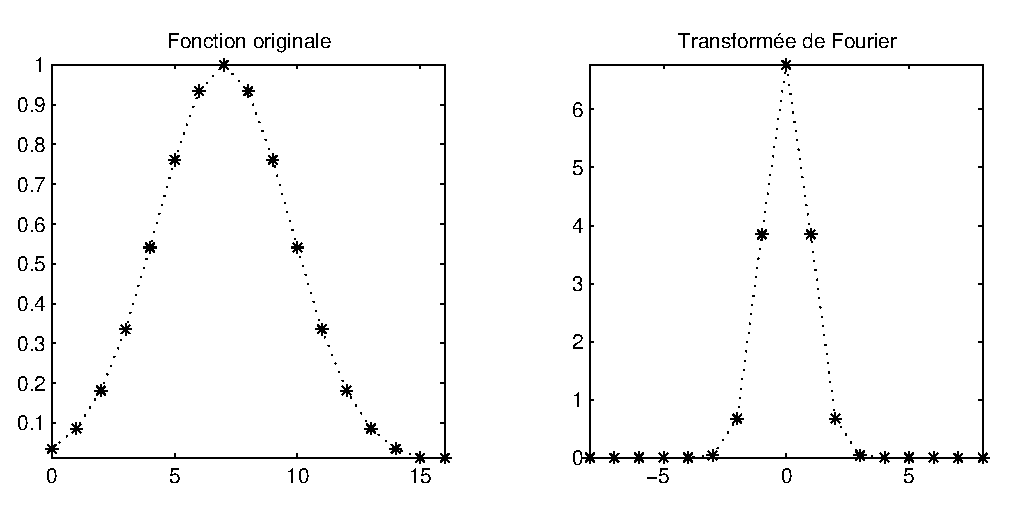
\includegraphics[scale = 0.7]{images/decomposition-fourier.eps}
    \end{center}
    \caption{Example of Fourier transform}
\label{fig-decomposition-fourier}
\end{figure}


\begin{rem}
The morphisms $ c $ and $\Ff $ are of course linear, so they are morphisms of vector spaces from $\CC[G]$ into $\CC[\wh{G}]$. They are in fact \textit{isomorphisms} of vector spaces, and to demonstrate this we will use the following Fourier inversion formula.
\end{rem}


\begin{prop}[Inversion formula]
\label{prop-decomposition-serie-fourier}
\index{Fourier!series} \index{Inversion!formula} For $ f \in \CC[G]$, we have the inversion formula
\begin{equation}
\label{eq-decomposition-serie-fourier-grpe-abelien}
f = \sum_{\chi \in \wh{G}}{c_f(\chi) \chi} = \frac{1}{|G|} \sum_{\chi \in \wh{G}}{\wh{f}(\chi) \chi^{-1}}.
\end{equation}

\end{prop}
\begin{proof}
The equation \eqref{eq-decomposition-serie-fourier-grpe-abelien} results immediately from the fact that $\wh{G}$ is an orthonormal basis of $\CC[G]$, by decomposing $f$ in this based.
\end{proof}


\begin{prop}[Fourier isomorphism]
$ c $ and $\Ff $ are isomorphisms of vector spaces from $\CC[G]$ into $\CC[\wh{G}]$.
\end{prop}
\begin{proof}
Let us show that $ c $ is injective. If $ c_f = 0 $, then the inversion formula \eqref{eq-decomposition-serie-fourier-grpe-abelien} shows that $ f = 0 $. As $G$ and $\wh{G}$ have the same cardinal (proposition \ref{cor-order-dual-equal-order-group}) the spaces $\CC[G]$ and $\CC[\wh{G}]$ have the same dimension $|G| = |\wh{G}|$. We therefore conclude that $ c $ is indeed an isomorphism. The reasoning is the same for $\Ff $.
\end{proof}


\begin{rem}
In reality, $\Ff $ is more than an isomorphism of vector spaces, since it also preserves a very particular algebra structure, the one defined by the convolution product. All this is the subject of Paragraph~\ref{sect2-convolution-transforme-fourier}.
\end{rem}
For now, let's continue to state the formulas that we get by using the decomposition in the base of characters.

\begin{prop}[Plancherel formula]
\label{prop-formula-floorel}
\index{Plancherel's formula} For $ (f, \, g) \in \CC[G]^2 $ we have the following formulas:
\begin{align}
\label{eq-formula-floorel-grpe-abelien-1}
\sum_{s \in G}{f (s) \ol{g (s)}} & = |G|\sum_{\chi \in \wh{G}}{c_{f}(\chi) \ol{c_{g}(\chi)}} \\
\label{eq-formula-floorel-grpe-abelien-2}
& = \frac{1}{|G|} \sum_{\chi \in \wh{G}}{\wh{f}(\chi) \ol{\wh{g}(\chi)}}.
\end{align}

\end{prop}
\begin{proof}
By decomposing $f$ and $g$ in the form $f(s) = \sum_{\chi \in \wh{G}}{c_{f}(\chi) \chi(s)}$ as well as $g(s) = \sum_{\chi \in \wh{G}}{c_{g}(\chi) \chi(s)}$, he comes
\begin{equation*}
\sum_{s \in G}{f (s) \ol{g (s)}} = |G|\dotp{f}{g} = |G|\sum_{(\chi_1, \, \chi_2) \in \wh{G}^2}{c_{f}(\chi_1) \ol{c_{g}(\chi_2)} \dotp{\chi_1}{\chi_2}}.
\end{equation*}
Hence the equation \eqref{eq-formula-floorel-grpe-abelien-1} using the orthogonality relations between characters. We prove in the same way the equation \eqref{eq-formula-floorel-grpe-abelien-2}.
\end{proof}


\begin{rem}{(\upshape \textbf{Link with theory $\mbold{L^2}$}).}
This formula is in every way similar to the formula that we obtain for the Fourier transform of two functions of $L^2(\RR)$. It translates the conservation of the scalar product (up to a constant) by the Fourier transform, since we can rewrite it in the form:
\begin{equation*}
\forall (f, \, g) \in \CC[G]^2, \quad \dotp{f}{g} = \frac{1}{|G|} \dotp{\wh{f}}{\wh{g}},
\end{equation*}
the second scalar product being of course that of $\CC[\wh{G}]$. This will be explained in detail in Section~\ref{sect1-link-trans-fourier-R}, where we discuss the link between the Fourier transform on the vectors of $\CC^N $ (called \textit{transform discrete}) and the Fourier transform \textit{continue}.
\end{rem}

% ------------------------------------------------- -----
% ------------------------------------------------- -----
% sub-section - Algebra of an abelian group
% ------------------------------------------------- -----
% ------------------------------------------------- -----
\subsection{Algebra of an abelian group}
\label{sect2-algebre-grpe-abelien}


\index{Product!term to term} \index{Convolution product} $G$ always designates a finite abelian group. Since the beginning of this talk, we have denoted $\CC[G]$ the (vector) space of functions from $G$ in $\CC$. We can give it an algebra structure thanks to the product of functions defined as follows:
\begin{equation}
\label{eq-defn-prod-term-term-functions}
\forall (f_1, \, f_2) \in \CC[G]^2, \; \forall g \in G, \quad (f_1 \cdot f_2)(g) \eqdef f_1(g) f_2(g).
\end{equation}
However, it is not this structure that will be useful for the following, but rather the one defined by the convolution product. Indeed, as we will see, the convolution product closely depends on the structure of the group $G$ considered, unlike the term-to-term product defined by the equation \eqref{sect2-convolution-transforme-fourier}. We will thus see in Paragraph~\ref{sect2-convolution-transforme-fourier} that the Fourier transform behaves in a very pleasant way for the convolution product.


\index{Algebra!of a group} We have already seen (to the proposition \ref{prop-base-c-g}) that a basis of the vector space $\CC[G]$ is given by the functions $\{\delta_g\}_{g \in G}$, where the function $\delta_G$, for $g \in G$, checks $\delta_g(g) = 1$ and $\delta_g(h) = 0 $ for $ h \in G$ such that $g \neq h$. Similarly, we have seen that a function $ f \in \CC[G]$ decomposes in the base $\{\delta_g\}_{g \in G}$ in
\begin{equation*}
f = \sum_{g \in G}{f(g) \delta_g}.
\end{equation*}
We then inject the group $G$ into the vector space $\CC[G]$ via the application
\begin{equation*}
j: g \in G \mapsto \delta_g \in \CC[G].
\end{equation*}
This allows to define (by structure transport) a multiplication noted $ *$ between the elements $\{\delta_g\}_{g \in G}$:
\begin{equation*}
\forall (g, \, h) \in G^2, \quad \delta_g * \delta_h \eqdef \delta_{g h}.
\end{equation*}
All that remains is to extend this multiplication to $\CC[G]$ by bilinearity in order to provide $\CC[G]$ with an algebra structure. This product is called the convolution product, and we can easily calculate the formula giving the expression of a product of two functions.

\begin{defn}[Convolution product]
\index{Convolution product} \label{notation-23} For $ f_1$ and $ f_2 $ two functions of $\CC[G]$, the convolution product $ f_1 * f_2 $ is given by
\begin{equation}
\label{eq-formula-prod-convol-grpe-abelien}
\forall g \in G, \quad (f_1 * f_2)(g) \eqdef \sum_{\scriptsize \begin{array}{c} (h, \, k) \in G^2 \\hk = g \end{array}}{f_1(h) f_2 (k)} = \sum_{h \in G}{f_1(h) f_2 (h^{-1} g)}.
\end{equation}

\end{defn}


\begin{rem}
For $ f \in \CC[G]$ we have
\begin{equation*}
\forall (g, \, h) \in G^2, \quad (f * \delta_g)(h) = f (h g^{-1}).
\end{equation*}
Thus the convolution by an element of $G$ (that is to say the convolution by a function $\delta_g$, using the identification) corresponds to a translation of the function. These properties will be explained again in the simple framework of $ G = \ZZ/n\ZZ$ in Section~\ref{sect1-tfd-prod-convol}. Let us content ourselves with stating the first properties of the convolution product.
\end{rem}


\begin{prop}
The convolution product is commutative, associative, and the map $ (f_1, \, f_2) \mapsto f_1 * f_2 $ is bilinear. We thus endow the vector space $\CC[G]$ with an algebra structure.
\end{prop}
\begin{proof}
The commutativity is easily verified by making the change of variable $ h'= h^{-1} g$ in the sum of the equation \eqref{eq-formula-prod-convol-grpe-abelien}. Associativity can be demonstrated by hand, or by using the \ref{thm-convolution-trans-fourier-grpe-abelien} theorem. The rest is easy.
\end{proof}
Before continuing, let's see \guill{graphically} what a convolution product looks like. Figure \figref{fig-convolution-intro} shows the convolution product with itself of a \guill{gate} function, on $\ZZ/16 \ZZ$. On the x-axis, we noted $\{0, \ldots, \, 15\}$ of the representatives of $\ZZ/16 \ZZ$. \begin{figure}[ht]
    \begin{center}
    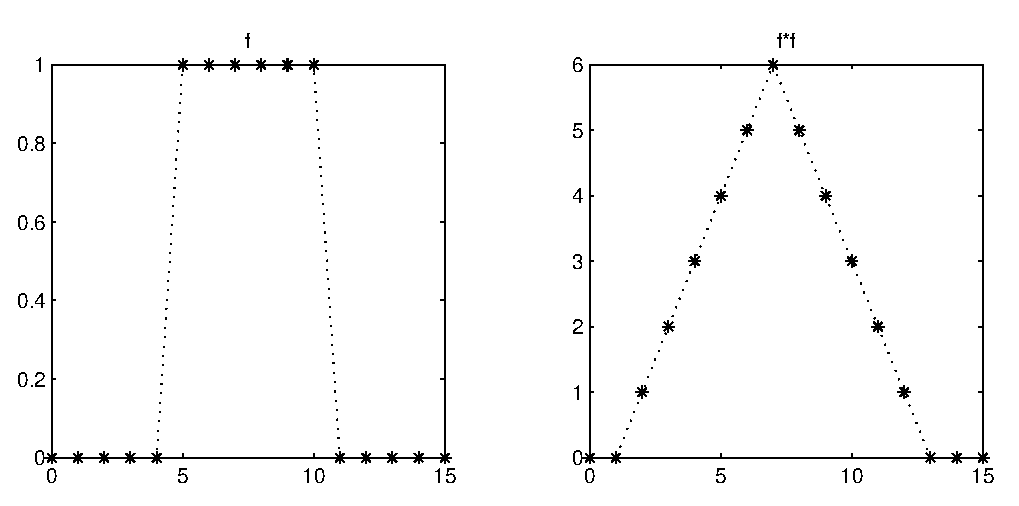
\includegraphics[scale = 0.7]{images/convolution-intro.eps}
    \end{center}
    \caption{Example of convolution calculation}
\label{fig-convolution-intro}
\end{figure}
This is the first time that we approach this kind of figures. These can be a bit confusing and the results aren't necessarily obvious. There are several possibilities. \begin{rs}
\item We can do the calculation by hand, and check that we get a \guill{triangle} function.
\item \index{Convolution!circular} We can expect the Section~\ref{sect1-tfd-prod-convol}, which studies in detail the discrete cyclic convolution. We will then be able to do the calculations with \Matlab{}, using the FFT algorithm.
\item We can read the Section~\ref{sect1-calculations-products}, which explains the link between the convolutional calculation and the multiplication of polynomials modulo $ X^n-1$.
\end{rs}


The fact that the convolution product is defined by extension of the product of the elements of $G$ allows us to state the following proposition.

\begin{prop}[Algebra morphism]
\label{prop-extension-morphism-grpe-algebra}
Let $\rho: G \rightarrow \CC^*$ be a group morphism. There is a unique way to extend it to an algebra morphism $\wt{\rho}: \CC[G] \rightarrow \CC$.
\end{prop}
\begin{proof}
Indeed, the construction of $\CC[G]$ tells us that $\wt{\rho}$ is only determined by the data of the values of $\wt{\rho}(\delta_g)$, for $ g \in G$. Now in the identification of $G$ as the canonical basis of $\CC[G]$, we have $\wt{\rho}(\delta_g) = \rho(g)$, which shows the uniqueness of the construction. It suffices then to show that the constructed morphism is indeed an algebra morphism. By definition of the convolution product, we can be satisfied with showing the conservation of the product over the elements $\{\delta_g\}_{g \in G}$, which is equivalent to the fact that $\rho$ is a morphism of group.
\end{proof}
This proposition tells us that there is a perfect correspondence between morphisms of groups of $G$ in $\CC^*$ and morphisms of algebras of $\CC[G]$ in $\CC$.

\begin{rem}{(\upshape \textbf{Probabilistic interpretation}).}
\label{rmk-interpretation-proba}
\index{Probability} The convolution product, which was introduced as the linear extension of a group operation, has a very important probabilistic interpretation. Let $ X $ and $ Y $ be two \textit{independent} random variables with values in a commutative finite group $G$. We denote by $ P_X $ and $ P_Y $ the corresponding probability distributions, that is to say $\forall g \in G, \; P_X(g) = \PP(\{X = g\})$. The fundamental result is that the probability distribution of the random variable $ X + Y $ is the convolution product of the distributions of $ X $ and $ Y $. This is therefore written $ P_{X + Y} = P_X * P_Y $. This theorem extends to continuous (with values in $\RR $) and discrete (with values in $\ZZ$) variables, provided that the appropriate convolution product is used. This result is very easy to show (the reader can verify it immediately), and we can consult \cite{ouvrard-2} on the applications of the convolution product in probability (in the continuous and discrete framework). The exercises \oldref{exo-repartition-proba} and \oldref{exo-marche-aleatoire} study the use of the Fourier transform on a finite group to solve probability problems.
\end{rem}

% ------------------------------------------------- -----
% ------------------------------------------------- -----
% sub-section - Convolution and Fourier transform
% ------------------------------------------------- -----
% ------------------------------------------------- -----
\subsection{Convolution and Fourier transform}
\label{sect2-convolution-transforme-fourier}


Let $G$ be a commutative finite group of order $n$. The following proposition shows that the definition of the Fourier transform is in fact very natural.

\begin{prop}[Algebra morphism]
\label{prop-thm-convol-fourier-grpe-finite}
Let $\chi \in \wh{G}$. The application
\begin{equation*}
\Ff_ \chi: \func{\CC[G]}{\CC}{f}{\wh{f}(\chi)}
\end{equation*}
corresponds to the unique way to extend the group morphism $\chi$ into an algebra morphism.
\end{prop}

\begin{proofnoqed}
The uniqueness results directly from the proposition \ref{prop-extension-morphism-grpe-algebra}. It only remains to show on the elements $\delta_G$ that $\Ff_ \chi$ corresponds to $\chi$, which is trivial:
\begin{equation*}
\forall g \in G, \quad \Ff_ \chi(\delta_g) = \sum_{x \in G}{\delta_g (x) \chi(x)} = \chi(g). \tag*{\qed}
\end{equation*}
\end{proofnoqed}

This property, which a posteriori justifies the introduction of the Fourier transform, is of capital importance, and we can summarize it in the form of the following convolution theorem.

\begin{thm}[Convolution and Fourier transform]
\label{thm-convolution-trans-fourier-grpe-abelien}
For $f$ and $g$ two functions of $\CC[G]$ we have
\begin{equation}
\label{eq-formula-convolution-functions-abelien-grpe}
\wh{f * g} = \wh{f} \cdot \wh{g} \quad \text{and} \quad c_{f * g} = |G| c_f \cdot c_g,
\end{equation}
where we denote by $\cdot $ the term-to-term product of two functions. The Fourier transform $\Ff $ is therefore an algebra isomorphism from $(\CC[G], \, *)$ to $(\CC[\wh{G}], \, \cdot)$.
\end{thm}



\index{Determinant!circulating} This convolution property is undoubtedly the
most used property of the Fourier transform, since it allows to change a rather
complex problem (the computation of a convolution of two functions) into a more
simple one (the calculation of the product term by term). The occurrences of this principle of simplification will be numerous throughout the book, whether they are theoretical studies (calculation of circulating determinant, Poisson's formula, etc.) or much more applied (filtering, product of large integers, decoding corrective codes, etc.).
% ------------------------------------------------- -----
% ------------------------------------------------- -----
% ------------------------------------------------- -----
% section - Exercises
% ------------------------------------------------- -----
% ------------------------------------------------- -----
% ------------------------------------------------- -----
\section{Exercises}
% \addcontentsline{toc}{section}{Exercises}
\label{sect1-chap1-exercises}

\begin{exo}[Circulating determinant]
\label{exo-determinant-circulating}

\index{Determinant!circulating} Let $G$ be a cyclic group. We fix $f \in \CC[G]$. We want to calculate the determinant of endomorphism
\begin{equation*}
\Phi^f \func{\CC[G]}{\CC[G]}{u}{f * u}.
\end{equation*}
We will often meet this type of application, in particular in Paragraph~\ref{sec2-linear-filters}, where it will be question of filtering. \begin{enumerate}
\item Explain why the elements $\chi \in \wh{G}$ are eigenvectors of $\Phi^f $. What are the associated eigenvalues?
\item What is the matrix $A$ of the endomorphism $\Phi^f $ in the base $\{\delta_g\}_{g \in G}$ of $\CC[G]$? Deduce from the previous question an expression of $\det (A)$.
\item By judiciously choosing the group $G$ and the application $f$, show that we have
\begin{equation*}
\det \begin{pmatrix} a_0 & a_1 & a_2 & \ldots & a_{n-1} \\a_{n-1} & a_0 & a_1 & \ldots & a_{n-2} \\vdots & \vdots & \vdots & & \vdots \\a_1 & a_2 & a_3 & \ldots & a_{0} \end{pmatrix} = \prod_{i = 0}^{n-1} \left(\sum_{j = 0}^{n-1}{a_j} \omega^{ij} \right),
\end{equation*}
where $ (a_0, \ldots, \, a_{n-1}) \in \CC^n $, and $\omega \eqdef e^{\frac{2 \imath \pi}{n}}$ (A such determinant is called \textit{circulating determinant}).
\item After having read the chapter \oldref{chap-tfd} devoted to the discrete Fourier transform and the FFT algorithm, propose a fast implementation of the circulating determinant calculus.
\end{enumerate}
\end{exo}


\begin{exo}[Dual of $\mbold{SO(3)}$]
\label{exo-dual-so3}

\index{Rotation} We denote by $SO(3)$ the group of real, orthogonal $ 3 \times 3 $ matrices with determinant 1. It corresponds to the rotations of $\RR^3 $. We want to show that $SO(3)$ has no non-trivial character. \begin{enumerate}
\item Show that two rotations of the same angle are conjugate.
\item Let $\chi$ be an element of the dual of $ SO(3)$. For $g \in SO(3)$, show that $\chi(g)$ depends only on the angle of $g$.
\item We denote by $r_{\alpha}$ the angle rotation $\alpha$ around $ (1, \, 0, \, 0)$, and $ s_{\alpha}$ the angle rotation $\alpha$ around $ (0, \, 1, \, 0)$. We consider $t_{\beta} \eqdef r_{\alpha} s_{\alpha}^{-1}$. Show that $t_{\beta}$ is a rotation of some angle $\beta $, and that when $\alpha$ traverses $[0, \, \pi]$, then $\beta $ does the same.
\item Deduce that $\chi = $ 1.
\end{enumerate}
\end{exo}


\begin{exo}[Enumeration of solutions]
\label{exo-enombrement-solutions}

\index{Enumeration} Let G be a finite abelian group, and a function $\varphi: G^n \rightarrow G$. For $ h \in G$, we denote by $ N(h)$ the number of $n$ -uples $ (g_1, \ldots, \, g_n)$ such that $\varphi (g_1, \ldots, \, g_n ) = h $. Show that we have
\begin{equation*}
N(h) = \frac{1}{|G|} \sum_{g_1 \in G}{\cdots \sum_{g_n \in G}{\sum_{\chi \in \wh{G}}{\chi \left(\varphi (g_1, \ldots, \, g_n) \right) \ol{\chi}(h)}}}.
\end{equation*}

\end{exo}


\begin{exo}[Indicator functions]
\label{exo-indicator-functions}

\index{Function!indicator} Let $G$ be a finite abelian group and $ A \subset G$. We denote by $ f_A $ the indicator function of $A$. \begin{enumerate}
\item Show that
\begin{equation*}
\norm{f_A}_2 = \sqrt{\frac{|A|}{|G|}} \quad \quad \text{et} \quad \quad \wh{f_A}(\chi_0) = |A|,
\end{equation*}
where we noted $\chi_0 $ the trivial character.
\item We assume that $|A|\leq \frac{1}{2}|G|$. We define
\begin{equation}
\label{eq-defn-phi-ensemble}
\Phi(A) \eqdef \max \enscond{|\wh{f_A}(\chi)|}{\chi \in \wh{G}, \; \chi \neq \chi_0}.
\end{equation}
Show that we have
\begin{equation}
\label{eq-ineq-regularity-function-indic}
\sqrt{\frac{|A|}{2}} \leq \Phi(A) \leq |A|.
\end{equation}

\item We take the case where $|A| > \frac{1}{2}|G|$. Show that we have $\Phi(A) = \Phi(G \backslash A)$, where we have denoted $ G \backslash A $ the complement of $A$ in $G$. Deduce a lowering of $\Phi(A)$ similar to \eqref{eq-ineq-regularity-function-indic}.
\item Show that if $\alpha$ is an automorphism of $G$, then $\Phi(\alpha (A)) = \Phi(A)$.
\end{enumerate} Intuitively, the closer $\Phi(A)$ is to the lower bound, the more the elements of $A$ are evenly distributed in $G$. The exercise \oldref{exo-repartition-proba} studies and quantifies this phenomenon. We can see an analogy with the study of the Fourier transform of a continuous function: the lower the high frequency Fourier coefficients, the more \guill{smooth} the function. These indicator functions will be used in Section~\ref{sect1-applications-correctors-codes} in the context where $A$ is used as corrective code. Once again, it is the spectral properties of $ f_A $ that will be used to study the \guill{geometry} of the set $A$.
\end{exo}


\begin{exo}[Equations on a finite abelian group]
\label{exo-eqn-grpe-abelien-finite}

\index{Equation!on an abelian group} This exercise uses the notations and results of exercise \oldref{exo-indicator-functions}. It is taken from the review article by Babai{\upshape \cite{babai-fourier-equations}}. \begin{enumerate}
\item We consider $ A_1, \ldots, \, A_k \subset G$, and we study the equation
\begin{equation}
\label{eq-exo-nbr-solution-eqn-grpe-finite}
x_1 + \cdots + x_k = a \quad \quad \text{with} \quad x_i \in A_i, \quad i = 1, \ldots, \, k.
\end{equation}
Explain how we can be reduced to the case $ a = 0 $. We denote by $n$ the number of solutions of \eqref{eq-exo-nbr-solution-eqn-grpe-finite}, in the case $ a = 0 $. Using the result of the exercise \oldref{exo-enombrement-solutions}, show that
\begin{equation*}
N = \frac{1}{|G|} \sum_{\chi \in \wh{G}}{\sum_{x_i \in A_i}{\chi(x_1 + \cdots + x_k)}} = \frac{| A_1 |\cdots | A_k |}{|G|} + R,
\end{equation*}
with
\begin{equation*}
R \eqdef \frac{1}{|G|} \sum_{\chi \neq \chi_0}{\prod_{i = 1}^k{\wh{f_{A_i}}(\chi)}}.
\end{equation*}

\item \index{Cauchy-Schwartz inequality} We assume that $ k = 3 $. To show that
\begin{equation*}
| R |\leq \frac{\Phi(A_3)}{|G|} \sum_{\chi \in \wh{G}}{|\wh{f_{A_1}}(\chi) | |\wh{f_{A_2}}(\chi) |} \leq \Phi(A_3) \sqrt{| A_1 | | A_2 |},
\end{equation*}
where $\Phi $ is defined by the equation \eqref{eq-defn-phi-ensemble} (we can use the Cauchy-Schwartz inequality). Show, using the result of the exercise \oldref{exo-indicator-functions}, question 4., that this is still valid when $ a \neq 0 $.
\item Deduce that if
\begin{equation*}
\frac{\Phi(A_3)}{| A_3 |} <\frac{\sqrt{| A_1 | | A_2 |}}{|G|},
\end{equation*}
then the equation $ x_1 + x_2 + x_3 = a $, with $ x_i \in A_i $, $ i = 1, \, 2, \, 3 $, has at least one solution.
\end{enumerate} This surprising result therefore tells us that if at least one of the three sets $ A_i $ is well distributed, and if the three sets are sufficiently large, then the considered equation has at least one solution. The exercise \oldref{exo-thm-fermat-finite-body} applies this result to $ G = \FF_q $ to study Fermat's theorem on finite fields.
\end{exo}


\begin{exo}[Heisenberg group]
\label{exo-groupe-heisenberg}

\index{Heisenberg's!group} Let $G$ be a finite abelian group. We denote by $\Uu $ the group of complex numbers of modulus $ 1$. We denote by $\Hh(g) \eqdef \Uu \times G \times \wh{G}$ provided with the operation
\begin{equation*}
(\lambda, \, x, \, \chi) \cdot(\mu, \, y, \, \tau) =(\lambda \mu \tau (x), \, xy, \, \chi \tau )
\end{equation*}
the Heisenberg group associated with $G$. \begin{enumerate}
\item Show that we define a group structure in this way. In particular, what is the neutral element and what is the inverse of a generic element $(\lambda, \, x, \, \chi) \in \Hh(g)$?
\item Show that we can define an action of $\Hh(g)$ on $\CC[G]$ by setting
\begin{equation*}
\forall f \in \CC[G], \; \forall(\lambda, \, x, \, \chi) \in \Hh(g), \quad(\lambda, \, x, \, \chi) \cdot f: z \mapsto \lambda \chi( z) f (xz).
\end{equation*}

\item \index{Translation} For $(\lambda, \, x, \, \chi) \in \Hh(g)$ and $ f \in \CC[G]$, we define respectively the expansion operators, translation, and modulation by
\begin{equation*}
D_ \lambda (f) (z) = \lambda f (z), \quad \quad T_x (f) (z) = f (xz), \quad \quad M_ \chi(f) (z) = \chi(z) f (z).
\end{equation*}
Express the action of $\Hh(g)$ on $\CC[G]$ in terms of these three operators. How do these three operators behave with respect to the Fourier transform defined in the equation \eqref{eq-transf-fourier-grpe-abelien}? What is the link with the continuous Fourier transform on $\RR $?
\item \index{Bidual} By canonically identifying $G$ to $\whwh{G}$ as described in Paragraph~\ref{sect2-bidual}, how the product on $\Hh(\wh{G}) = \Uu \times \wh{G} \times G$ defined? How to define an action of $\Hh(\wh{G})$ on $\CC[\wh{G}]$?
\item We define the function
\begin{equation*}
\alpha: \func{\Hh(g)}{\Hh(\wh{G})}{(\lambda, \, x, \, \chi)}{(\lambda \chi^{-1} ( x), \, \chi, \, x^{-1})}.
\end{equation*}
Show that $\alpha$ is an isomorphism of groups, and that we have
\begin{equation*}
\forall f \in \CC[G], \; \forall(\lambda, \, x, \, \chi) \in \Hh(g), \quad \Ff \left((\lambda, \, x, \, \chi) \cdot f \right) = \alpha(\lambda, \, x, \, \chi) \cdot \Ff (f),
\end{equation*}
where $\Ff $ denotes the Fourier transform defined in the equation \eqref{eq-transf-fourier-grpe-abelien}.
\item \index{Lemma!of Schur} We suppose that $\Phi: \CC[G] \rightarrow \CC[G]$ commutes with the action of $\Hh(g)$, that is say that
\begin{equation*}
\forall f \in \CC[G], \; \forall(\lambda, \, x, \, \chi) \in \Hh(g), \quad \Phi((\lambda, \, x, \, \chi) \cdot f) =(\lambda, \, x, \, \chi) \cdot \Phi(f).
\end{equation*}
Show that there exists $ r \in \CC^*$ such that $\forall f \in \CC[G], \; \Phi(f) = r f $. We can reason on the matrix of $\Phi $ expressed in the base $\{\delta_g\}_{g \in G}$ of $\CC[G]$, or then use Schur's lemma \ref{lemma-schur}. What happens if $\Phi: \CC[G] \rightarrow \CC[\wh{G}]$ switches the actions of $\Hh(g)$ and $\Hh(\wh{G})$?
\end{enumerate}
\end{exo}


\begin{exo}[Fourier transform and orthogonalization]
\label{exo-series-fourier-orthogonalisation}

\index{Orthogonalization} \index{Translation} We consider a function $ f \in L^2(\RR)$. We denote by $\tau_r $ the translation of $ r $ on $L^2(\RR)$, i.e. $\tau_r (f) = f(\cdot-r)$. \begin{enumerate}
\item Show that the family $\{\tau_n (f)\}_{n \in\ZZ}$ is orthonormal if and only if
\begin{equation*}
\text{for a.e. } \omega \in \RR, \quad \sum_{k \in\ZZ}{|\wh{f}(\omega + 2k \pi) |^2} = 1,
\end{equation*}
where we have denoted $\wh{f} \in L^2(\RR)$ the Fourier transform of $f$, defined, for the functions $ f \in L^1(\RR)$ by
\begin{equation*}
\text{for a.e. } \omega \in \RR, \quad \wh{f}(\omega) \eqdef \int_{\RR}{f (x) e^{- \imath \omega x} \d x},
\end{equation*}
and extended by density to $L^2(\RR)$ whole.
\item \label{notation-24} We assume that there exists $ A> 0 $ such that
\begin{equation*}
\text{for a.e. } \omega \in \RR, \quad A \leq \sum_{k \in\ZZ}{|\wh{f}(\omega + 2k \pi) |^2}.
\end{equation*}
Show that if we denote by $\varphi $ the function of $L^2(\RR)$ such that
\begin{equation*}
\text{for a.e. } \omega \in \RR, \quad \wh{\varphi}(\omega) \eqdef \frac{\wh{f}(\omega)}{\left(\sum_{k \in\ZZ}{|\wh{f}(\omega + 2k \pi) |^2} \right)^{1/2}},
\end{equation*}
then the family $\{\tau_n(\varphi)\}_{n \in\ZZ}$ is orthonormal (equalities are to be considered for almost all $\omega $).
\end{enumerate} The following exercise \oldref{exo-orthogonalization-abelian-group} proposes to study the same orthogonalization problem, but within the framework of a finite abelian group.
\end{exo}

\begin{exo}[Orthogonalization on an abelian group]
\label{exo-orthogonalization-abelian-group}

\index{Orthogonalisation} \index{Transformation!group} \index{Unitary!endomorphism} This exercise is inspired by the article by \nompropre{Bernardini} and \nompropre{Kovacevic}{\upshape \cite{bernardini-orthogonalisation-1}}. Let $ V $ be a $\CC$ -vector space of dimension $n$, endowed with a Hermitian product $\dotp{\cdot}{\cdot}$. Let $G$ be a finite abelian group of unit transformations of $ V $, and let $ b \in V $. We say that $ b $ is orthonormal for the action of $G$ on $ V $ if the set $ G_b \eqdef \enscond{A b}{A \in G}$ is orthonormal. This means that
\begin{equation*}
\forall (x, \, y) \in G_b^2, \quad \dotp{x}{y} = \delta_x^y.
\end{equation*}
\begin{enumerate}
\item We note
\begin{equation*}
\psi_b: \func{G}{\CC}{A}{\dotp{A b}{b}}.
\end{equation*}
Show that $ b $ is orthonormal for the action of $G$ if and only if $\wh{\psi_b} \equiv 1$, i.e. if and only if $\forall \chi \in \wh{G}$, $|G|\dotp{\Uu_ \chi b}{b} = $ 1, where we noted
\begin{equation*}
\forall \chi \in \wh{G}, \quad \Uu_ \chi \eqdef \frac{1}{|G|} \sum_{A \in G}{\chi(A) A} \quad \in \Ll (V, V).
\end{equation*}

\item Show that the operators $\Uu_ \chi$ are orthogonal projectors, and that they are two by two orthogonal, that is to say
\begin{equation*}
\forall(\chi_1, \, \chi_2) \in \wh{G}^2, \quad \Uu_{\chi_1} \Uu_{\chi_2} = \left\{\begin{array}{lll} 0 & \text{if} & \chi_1 \neq \chi_2 \\\Uu_{\chi_1} & \text{if} & \chi_1 = \chi_2 \end{array} \right.,
\end{equation*}
and $\Uu_ \chi^* = \Uu_ \chi$ ($ A^*$ denotes the assistant of $A$).
\item We assume that $\wh{\psi_b}$ does not vanish. We notice
\begin{equation*}
\wt{b} \eqdef \sum_{\chi \in \wh{G}}{\frac{1}{\sqrt{\wh{\psi_b}(\chi)}} \Uu_ \chi b},
\end{equation*}
where $\sqrt{\wh{\psi_b}(\chi)}$ denotes one of the two possible roots. Show that $\wt{b}$ is orthonormal for the action of $G$.
\item What connection can we make with the exercise \oldref{exo-series-fourier-orthogonalisation}?
\end{enumerate} For a more in-depth study of this method in the case of cyclic groups $\ZZ/n\ZZ$, we can look at the exercise \oldref{exo-series-fourier-orthogonalisation}.
\end{exo}


\begin{exo}[Distribution of probability]
\label{exo-repartition-proba}

\index{Probability} Let $G$ be a finite abelian group, and $ P: G \rightarrow \RR^+ $ the distribution function of a probability law on $G$, which means that $\sum_{g \in G}{P(g)} = $ 1. We denote by $ U $ the uniform distribution, that is to say $ U(g) = \frac{1}{|G|}$ for all $ g \in G$. We denote by $\chi_0 $ the trivial character of $G$. \begin{enumerate}
\item Calculate $\wh{P}(\chi_0)$ as well as $\wh{U}(\chi)$, for $\chi \in \wh{G}$. Deduce an expression of $\norm{P - U}_2^2 $.
\item Show that we have
\begin{equation*}
\forall g \in G, \quad \left| P(g) - \frac{1}{|G|} \right|^2 \leq \frac{1}{|G|} \sum_{\chi \neq \chi_0}{|\wh{P} ( \chi) |^2}.
\end{equation*}

\end{enumerate} In a way, the quantity $\norm{P - U}_2^2 $ measures the uniformity of the distribution $ P $, and as we have already seen for the characteristic functions (exercise \oldref{exo-indicator-functions}), this is characterized by the Fourier coefficients $\wh{P}(\chi)$, for $\chi \neq \chi_0 $.
\end{exo}


\begin{exo}[Random walk]
\label{exo-marche-aleatoire}

\index{Random walk} \index{Probability} \index{Markov chain} \index{Transition matrix} We consider a random walk on $\ZZ/n\ZZ$ cons \-trui \-te as follows. The random variable $ X_k \in\ZZ/n\ZZ$ designates a position on the circle $\ZZ/n\ZZ$ at the instant $ k \in \NN $. The displacement between the instant $ k $ and $ k + 1$ is given by a transition probability $ p_{i, j} \eqdef \PP (X_{k + 1} = j \, |\, X_k = i )$. \begin{enumerate}
\item We denote by $ p^{(k)}: G \rightarrow [0, \, 1]$ the probability distribution of $ X_k $, i.e. for $0 \leq i <n $, $ p^{(k)} (i) = \PP (X_k = i)$. We can also write $ p^{(k)}$ in the form of a vector of size $n$. Show that $ p^{(k + 1)} = P p^{(k)}$, where we have denoted $ P $ the transition matrix $\{p_{i, j}\}_{0 \leq i, j \leq n-1}$. Deduce that $ p^{(k)} = P^kp^{(0)}$, where $ p^{(0)} = \{1, \, 0, \ldots, \, 0\}$ is the initial distribution.
\item Let $0 <p <1$. We consider the simplest random walk, given by
\begin{equation*}
\left\{\begin{array}{l} p_{i, i-1} = p, \quad \quad p_{i, i + 1} = 1-p, \\p_{i, j} = 0 \quad \text{if} \quad i \notin \{i-1, \, i + 1\} \end{array} \right. .
\end{equation*}
Show that we then have $ P x = v * x $, where $ *$ denotes the product of convolution and $ v = \{0, \, p, \, 0, \ldots, \, 0, \, 1-p\}$. How can we find this result by considering sums of random variables, and by using the remark \ref{rmk-interpretation-proba}?
\item Express the Fourier transform $\wh{p^{(k)}}$ from $\wh{p^{(0)}}$. Deduce that if $n$ is odd, then
\begin{equation*}
p^{(k)} \tv{k \to \pinf} u \quad \quad \text{where} \quad \quad u \eqdef \{1/n, \ldots, \, 1/n\}.
\end{equation*}
What happens if $n$ is even?
\item \index{Translation} Generalize this result to a translation invariant random walk, that is to say such that
\begin{equation*}
p_{i, j} = v_{j-i} \quad \quad \text{with} \quad \quad v \in ([0, \, 1])^n.
\end{equation*}

\end{enumerate} The figure \figref{fig-marche-aleatoire} shows the progression of the probability distribution $ p^{(k)}$ in the case of two random walks. We see that the second step converges more quickly towards the uniform distribution (we can make the link with the size of the Fourier coefficients). \begin{figure}[ht]
    \begin{center}
    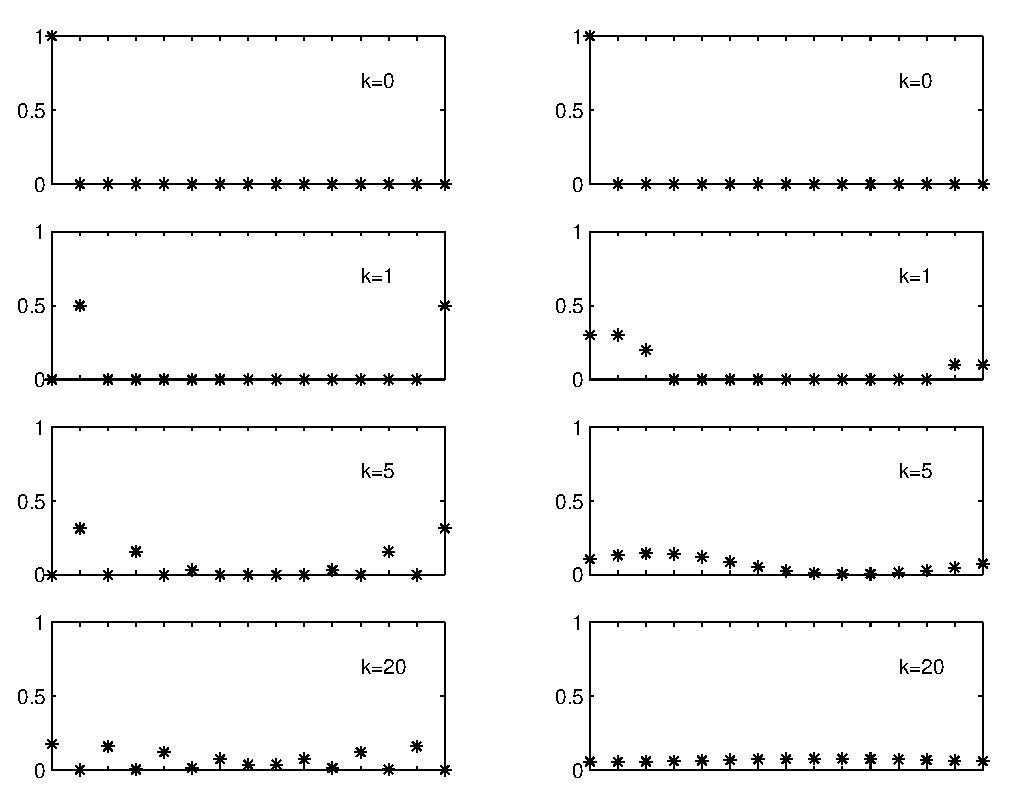
\includegraphics[scale = 0.6]{images/marche-aleatoire.eps}
    \end{center}
    \caption{Random walks for the transition probabilities $\{0, \, 1/2, \, 0, \ldots, \, 0, \, 1/2\}$ (left) and $\{0.3, \, 0.3, \, 0.2, \, 0, \ldots, \, 0, \, 0.1, \, 0.1\}$ (right)}
\label{fig-marche-aleatoire}
\end{figure}

\end{exo}


\begin{exo}[Discrete uncertainty principle]
\label{exo-principle-uncertainty-discrete}

\index{Uncertainty!principle} \index{Uncertainty} \index{Support} 
Let $G$ be a finite group, and $ f \in \CC[G]$ a non-zero function. We want to show that we have
\begin{equation}
	\label{eq-pcpe-uncertainty-discrete}
\big |\Supp (f) \big |\times \big |\Supp \big(\wh{f} \big) \big |\geq |G|,
\end{equation}
where $|\Supp (f) |$ denotes the size of the support of $f$. 
\begin{enumerate}
\item We consider, first of all, the group $ G = \ZZ/n\ZZ$. Show that if $f$ has $ p $ non-zero elements, then $\wh{f}$ cannot have $ p $ consecutive zeros. Deduce the equation \eqref{eq-pcpe-uncertainty-discrete}. This result was demonstrated first by \nompropre{Donoho} and \nompropre{Stark}{\upshape \cite{donoho-stark-uncertainty}}.
%%
\item \index{Cauchy-Schwartz inequality!} We return to the general case of a finite abelian group $G$. \\We denote by $ M \eqdef \sup \enscond{f (x)}{x \in G}$ and $\norm{f}_2^2 \eqdef \dotp{f}{f}$. To show that
\begin{equation*}
\norm{f}_2^2 \leq \frac{M^2}{|G|}|\Supp (f) |\quad \quad \text{et} \quad \quad M \leq \frac{1}{|G|} \sum_{\chi \in \wh{G}}{|\wh{f}(\chi) |}.
\end{equation*}
Using the Cauchy-Schwartz inequality, deduce that
\begin{equation*}
M^2 \leq \frac{|\Supp(\wh{f}) |}{|G|} \norm{\wh{f}}_ 2^2, \quad \quad \text{then,} \quad \quad M^2 \leq \norm{f}_2^2 |\Supp(\wh{f}) |.
\end{equation*}
To conclude that
\begin{equation*}
\norm{f}_2^2 \leq \frac{\norm{f}_2^2}{|G|}|\Supp (f) |\times |\Supp(\wh{f}) |.
\end{equation*}
%%%
\item \index{Subgroup} \index{Orthogonal!of a subgroup} Let $ H \subset G$, a subgroup and $ f_H \in \CC[G]$, its characteristic function. Show that we have
\begin{equation*}
\wh{f_H} = |H| f_{H^\sharp},
\end{equation*}
where we denote by $ H^\sharp \subset \wh{G}$ the orthogonal of $H$. Deduce that the function $f$ reaches the bound of the equation \eqref{eq-pcpe-uncertainty-discrete}. In fact, we can show that any function which reaches this bound is related to such a function $ f_H $ by a translation and a dilation. This is demonstrated in the article by \nompropre{Matusiak}{\upshape \cite{matusiak-donoho-stark}}.
\end{enumerate} 
This conclusion on the localization of temporal and frequency supports may seem negative at first glance: it prohibits us from constructing signals well localized both in time and in frequency. However, it can be used to advantage, for example to build efficient corrective codes, as the proposition \ref{prop-dist-minimal-code-bch} will show.
\end{exo}

 
\chapter{Applications of duality on a finite group}
\label{chap-applications-trans-fourier-grpe-finite} 
 
To better understand the theory of characters over a commutative group, it must be applied in situations where it is really useful. The aim of this chapter is therefore to understand, through examples, why this theory is so powerful. We will thus demonstrate without too much effort formulas that may seem complex, at least for someone who is approaching them for the first time. The best example is the quadratic reciprocity formula, the proof of which is based on the use of two types of characters.

% ------------------------------------------------- -----
% ------------------------------------------------- -----
% ------------------------------------------------- -----
% section - Gaussian sums                            
% ------------------------------------------------- -----
% ------------------------------------------------- -----
% ------------------------------------------------- -----
\section{Gaussian sums}
% \addcontentsline{toc}{section}{Gaussian sums}
\label{sect1-are-gauss} 
 
 

\index{Finite field} The idea behind the discussion of this paragraph is very simple. It is a matter of better understanding \textit{finite fields}, and more precisely, of perceiving more clearly how the two structures which make up such a field (multiplicative group and additive group) can co-exist, and influence each other mutually. The main tool will of course be the \textit{duality} on an abelian group, and the idea to develop will be the combination of two types of characters. It is precisely to combine these characters that we are going to introduce the notion of \textit{Gaussian sum}, which is presented in Paragraph~\ref{sect2-are-gauss}.
 
 
The main reference for this talk is the book of \nompropre{Lidl} and \nompropre{Niederreiter} \cite{lidl}, which constitutes a true encyclopedia of finite fields. We can also read with great interest the very nice presentation of \nompropre{Langevin} \cite{langevin}, which links many related subjects, such as Gaussian sums, corrective codes, and number theory.
% ------------------------------------------------- -----
% ------------------------------------------------- -----
% sub-section - Quadratic residues                            
% ------------------------------------------------- -----
% ------------------------------------------------- -----
\subsection{Quadratic residues}
 
\index{Quadratic residue} \index{Equation!over a finite field} Before embarking on the study of duality over a finite field, let us give a simple example which will justify the introduction of character theory. Consider the following equation, which has integer unknowns:
\begin{equation}
\label{eq-example-quadratic-equation}
x^2 = 2 y^2 + 7 k \quad \quad \text{with} \quad (x, \, y, \, k) \in \ZZ^3.
\end{equation}
To solve it almost trivially, we just need to replace it with its counterpart modulo the prime number $ 7 $, and use the field structure of $ \ZZ/7 \ZZ $ which allows us to perform divisions:
\begin{equation*}
\left(x / y \right)^2 = 2 \mod{7},
\end{equation*}
for $ x \neq 0 $. All that remains is to list the squares of $ \{0, \, 1, \ldots, \, 6\} $, taken modulo $ 7 $. We easily get $ \{0, \, 1, \, 4, \, 2, \, 2, \, 4, \, 1\} $. We therefore conclude that the non-zero solutions of the equation are given by
\begin{equation*}
\frac{x}{y} = 3 + 7k'\quad \text{and} \quad \frac{x}{y} = 4 + 7k', \quad \text{for} k'\in \ZZ.
\end{equation*}
Obviously, now that we know the square roots of 2 in $ \ZZ/7 \ZZ $, we can consider the following factorization of the equation \eqref{eq-example-quadratic-equation}:
\begin{equation*}
(x - 3 y) (x - 4 y) = 0 \mod{7},
\end{equation*}
which of course leads to the same result.
 
 
\index{Symbol!of Legendre} \index{Legendre@\nompropreindex{Legendre}} This naive approach is obviously to be avoided in the case of study of large numbers. We are led to consider, for a prime number $ p $ the \textit{Legendre symbol}, defined as follows: \label{notation-25}
\begin{equation*}
\forall n \in \ZZ, \quad \legsymb{n}{p} = \left\{\begin{array}{rl} 0 & \text{if
} n \text{ is divisible by } p \\1 & \text{if } n \text{ is a square modulo } p \\-1
				   & \text{if } n \text{ is not a square modulo } p \end{array} \right. .
\end{equation*}
It is obvious that we can restrict the study of this symbol to only the elements of $ \ZZ/p \ZZ $, which we usually denote by $ \FF_p $. The capital remark for what follows is that the application
\begin{equation}
\label{eq-defn-cartactere-eta}
\eta: \func{\FF_p^*}{\{- 1, \, 1\}}{n}{\legsymb{n}{p}}
\end{equation}
is a character of the multiplicative group $ \FF_p^* $, since we have
\begin{equation*}
\legsymb{n_1 n_2}{p} = \legsymb{n_1}{p} \legsymb{n_2}{p}.
\end{equation*}
This property follows directly from the following lemma.
 
\begin{lem}[Euler's formula]
\label{lem-formula-euler}
\index{Euler's formula!} \index{Euler@\nompropreindex{Euler}} Let $ p $ be an odd prime number. An element $ x \in \FF_p^* $ is a square if and only if $ x^{\frac{p-1}{2}} = $ 1. An element $ x \in \FF_p^* $ is not a square if and only if $ x^{\frac{p-1}{2}} = -1 $. Consequently, we have the formula of \textit{Euler}
\begin{equation*}
\forall x \in \FF_p^*, \quad \legsymb{x}{p} = x^{\frac{p-1}{2}}.
\end{equation*}
\end{lem}
 
\begin{proof}
We consider the multiplicative group $ \FF_p^* $. As $ p $ is odd, the morphism $ x \mapsto x^2 $ has as its kernel the subgroup $ \{1, \, - 1\} $, of so that the elements which are modulo $ p $ squares form a subgroup of $ \FF_p^* $ of cardinal $ \frac{p-1}{2} $. \\If $ x = y^2 $, then $ x^{\frac{p-1}{2}} = y^{p-1} = $ 1. So the $ \frac{p-1}{2} $ quadratic residues modulo $ p $ are all roots of the polynomial $ X^{\frac{p-1}{2}} - 1 $, which cannot have more than $ \frac{p-1}{2} $ roots. The residuals are therefore exactly these roots, that is to say the elements $ x $ such that $ x^{\frac{p-1}{2}} = 1 $. \\To conclude the demonstration, it suffices to note that $ \left(x^{\frac{p-1}{2}} \right)^2 = 1 $ implies that $ x^{\frac{p-1}{2}} $ is an element of $ \{- 1, \, 1\} $. The quadratic non-residues are characterized by $ x^\frac{p-1}{2} = -1 $, which completes the proof of Euler's formula.
\end{proof}
The aim of this chapter is to demonstrate the important property of these Legendre characters, which we call the quadratic reciprocity formula. It relates the fact of being a square modulo $ p $ to that of being a square modulo $ q $. In his time, \textit{Euler} had already noticed, by calculating many cases by hand, that for two first distinct odd numbers $ p $ and $ q $, we have $ \legsymb{p}{q} = \legsymb{q}{p} $, except in the case where $ p $ and $ q $ are both of the form $ 4 k - 1 $. This result is however far from obvious, and it was necessary to wait \textit{Gauss} to obtain a complete proof of this result.
 
 
Thanks to this formula, we will be able to easily calculate the Legendre character, by successively applying inversions of the symbol $ \left(\frac{q}{p} \right) $ (with the reciprocity formula) and reductions of $ q $ modulo $ p $ (because the symbol depends only on the class of $ n $ modulo $ p $).
% ------------------------------------------------- -----
% ------------------------------------------------- -----
% sub-section - Additive and multiplicative characters                            
% ------------------------------------------------- -----
% ------------------------------------------------- -----
\subsection{Additive and multiplicative characters}
 
 
In the previous chapter, we were interested in commutative finite groups. We are now going to impose a more rigid structure on our group, since we are going to be interested in a finite field $ \FF_q $, with $ q = p^r $ where $ p $ is a prime number. It is a feature field $ p $, and it can be seen as a finite dimensional vector space $ r $ over its prime field $ \FF_p $. A more detailed description of finite fields will be given in Section~\ref{sect1-calculations-finite-field}, when constructing a Fourier transform with values in a finite field.
 
 
On our fied, we can identify two group structures. First of all we can consider $ \FF_q $ as an additive group (in fact a vector space on $ \FF_p $). Then, we can also consider the multiplicative group $ \FF_q^* \eqdef \FF_q - \{0\} $, which is a cyclic group of order $ q-1 $. This leads to considering two types of characters.
 
\begin{defn}[Additive and multiplicative characters]
\index{Additive!Character} \index{Multiplicative!Character} The elements of $ \wh{\FF_q} $ are called \textit{additive characters}. These are therefore the morphisms
\begin{equation*}
\psi: (\FF_q, \, +) \longrightarrow (\CC^*, \, *).
\end{equation*}
The elements of $ \wh{\FF_q^*} $ are called \textit{multiplicative characters}. These are therefore the morphisms
\begin{equation*}
\chi: (\FF_q^*, \, *) \longrightarrow (\CC^*, \, *).
\end{equation*}
\end{defn}
 
 
 
The easiest characters to determine are the multiplicative characters, that is, the elements of $ \wh{\FF_q^*} $. Indeed, the group $ \FF_q^* $ is cyclic. So let $ \zeta $ be a generator of this group, so that we have $ \FF_q^* = \{1, \, \zeta, \, \zeta^2, \ldots, \, \zeta^{q-2}\} $. We can then enumerate the $ q-1 $ multiplicative characters
\begin{equation*}
\forall j = 0, \ldots, \, q-1, \quad \chi_j: \func{\FF_q^*}{\FF_q^*}{\zeta^k}{e^{\frac{2 \imath \pi}{q-1} jk}}.
\end{equation*}
We thus obtain a complete description of the dual group $ \wh{\FF_q^*} $, and we see of course that we have $ \wh{\FF_q^*} \simeq \FF_q^* $. This description is not canonical, in the sense that it requires the (arbitrary) choice of a primitive root $ \zeta $.
 
 
Regarding the additive group $ \FF_q $, the situation is a little more complex, since this group is not cyclic. However, as an additive group, $ \FF_q $ is in fact isomorphic to the product group $ \left(\ZZ/p \ZZ \right)^r $. As $ \ZZ/p \ZZ $ is a cyclic (additive) group, it will be relatively easy to list the additive characters of $ \FF_q $. However, in order to produce as little effort as possible, and to simplify the description of the dual, we will introduce the following notion.
 
\begin{defn}[Application trace]
\index{Trace!of $ K $ in $ k $} \label{notation-26} Let $ K $ be a finite field,
containing a sub-field $ k $ of cardinality $ s $. We denote by $ t \eqdef [K: k] $ the dimension of $ K $ as $k$-vector space, so that $ | K | = s^t $. Let $ \alpha \in K $. We define the application \textit{trace} from $ K $ to $ k $ as follows:
\begin{equation*}
\Tr_{K / k} (\alpha) \eqdef \alpha + \alpha^s + \cdots + \alpha^{s^{t-1}}.
\end{equation*}
In the following, we will be interested in the bodies $ k = \FF_p $ and $ K = \FF_q $ (we therefore fix $ s = p $ and $ t = r $). When there is no risk of confusion, we will simply write $ \Tr $ instead of $ \Tr_{\FF_q / \FF_p} $.
\end{defn}
 
We recall some important properties of finite fields, which we will find demonstrated in the book of \nompropre{Perrin} \cite{perrin}.
 
\begin{prop}[Properties of finite fields]
Let $ K $ be a finite field of characteristic $ p $. \begin{itemize}
\item [{\upshape (i)}] Let $ k $ be a subfield of $ K $ of cardinal $ s $ An element $ x \in K $ belongs to $ k $ if and only if $ x^s = x $.
\item [{\upshape (ii)}] \index{Morphism!of Frobenius} \index{Frobenius@\nompropreindex{Frobenius}} The application $ \Phi: x \mapsto x^p $ is a morphism, called morphism by Frobenius. The iterates $ \Phi^k: x \mapsto x^{p^k} $ are also morphisms.
\end{itemize}
\end{prop}
 
Let's see the main properties of this application.
 
\begin{prop}[Track properties]
The trace of $ K $ over $ k $ is a non-zero $ k $ -linear form with values in $ k $.
\end{prop}
\begin{proof}
\index{Morphism!of Frobenius} The first thing to show is that for $ \alpha \in K $, we have $ \Tr_{K / k} (\alpha) \in k $. It suffices to show that we have $ x^s = x $. Using the linearity of the morphism $ x \mapsto x^s $ (which is an iterated from Frobenius), it comes
\begin{equation*}
\Tr_{K / k} (\alpha)^s = \alpha^s + \alpha^{s^2} + \cdots + \alpha^{s^t}.
\end{equation*}
Since $ K^* $ is a group of cardinal $ s^t-1 $, we have $ \forall \alpha \in K^*, \; \alpha^{s^t-1} = 1 $, hence the desired result, since $ \forall \alpha \in K, \; \alpha^{s^t} = \alpha $. \\Using the Frobenius morphism and the fact that $ \lambda^s = \lambda $ for a scalar $ \lambda \in k $, it is clear that l The trace application is indeed $ k $ -linear. It remains to show that it is not trivial, i.e. there exists an element $ \alpha \in K $ such that $ \Tr_{K / k} (\alpha) \neq 0 $. Now, if $ \Tr_{K / k} (\alpha) = 0 $, this means that $ \alpha $ is root of the polynomial
\begin{equation*}
P (X) \eqdef X + X^s + \cdots + X^{s^{t-1}},
\end{equation*}
which is of degree $ s^{t-1} $. This polynomial therefore has at most $ s^{t-1} $ roots, and as $ K $ a $ s^t $ elements, there does exist a certain $ \alpha \in K $ such that $ P (\alpha) \neq $ 0.
\end{proof}
 
We can now provide a full description of the additive characters of $ \FF_q $.
To do this, we introduce a so-called \textit{canonical} character, in the sense
that it is independent of the way in which we construct the field $ \FF_q $.
 
\begin{defn}[Canonical character]
\label{defn-character-additive-canonical}
\index{Character!canonical} \label{notation-27} We define the additive character \textit{canonical} $ \psi_1 $, element of $ \wh{\FF_q} $ by
\begin{equation*}
\psi_1: \func{\FF_q}{\CC^*}{x}{e^{\frac{2 \imath \pi}{p} \Tr (x)}}.
\end{equation*}
\end{defn}
 
The following theorem explains the construction of other characters from this canonical character.
 
\begin{prop}
\label{prop-characters-any-additives}
Let, for $ a \in \FF_q $, the application
\begin{equation*}
\psi_a: \func{\FF_q}{\CC^*}{x}{\psi_1 (ax)}.
\end{equation*}
It is an additive character, $ \psi_a \in \wh{\FF_q} $, and conversely, any additive character is written that way.
\end{prop}
 
\begin{proof}
It is obvious that we have well constructed characters in this way. Let us show that they are all different. \\Since the trace is non-identically zero, the canonical character is non-trivial. If we consider two elements $ a \neq b $ of $ \FF_q $, then we can find another element $ c \in \FF_q $ such that
\begin{equation*}
\frac{\psi_a (c)}{\psi_b (c)} = \psi_1 \left((ab) c \right) \neq 1.
\end{equation*}
So we have $ \psi_a \neq \psi_b $. This means that the number of characters of type $ \psi_a $ is equal to $ q $. Now we know, with Corollary~\ref{cor-order-dual-equal-order-group}, that $ | \wh{\FF_q} | = | \FF_q | = q $. We have therefore constructed all the characters well.
\end{proof}
 
 
\begin{rem}{(\upshape \textbf{Trivial character}).} 
\index{Character!trivial} We have thus constructed an isomorphism between $ \FF_q $ and its dual $ \wh{\FF_q} $ by the application $ a \mapsto \psi_a $. We denote by $ \psi_0 = 1 $ the trivial additive character. It should not be confused with the trivial multiplicative character $ \chi_0 $, since the latter is not defined in $ 0 $. We will see later that we often extend the multiplicative characters $ \chi \in \wh{\FF_q^*} $ by setting $ \chi (0) = 0 $, which removes any ambiguity between the two trivial characters.
\end{rem}
 
 
\begin{rem}{(\upshape \textbf{Character extension}).} 
Let $ K $ be a finite super-field of $ \FF_q $, which can be written in the form $ K = \FF_{q^t} $, where $ t \eqdef [K: \FF_q] $. We can easily check that for $ \beta \in K $, we have
\begin{equation*}
\Tr_{K / \FF_p} (\beta) = \Tr_{\FF_q / \FF_p} \left(\Tr_{K / \FF_q} (\beta) \right).
\end{equation*}
If we denote by $ \mu_1 $ the canonical character of $ K $, this implies that
\begin{equation}
\label{eq-formula-extension-canonical-car}
\mu_1 (\beta) = \psi_1 (\Tr_{K / \FF_q} (\beta)).
\end{equation}
\end{rem}
Before detailing the properties of additive and multiplicative characters, let us give a basic example.
 
\begin{exmp}[Quadratic character]
\index{Quadratic!character} \index{Symbol!of Legendre} \index{Legendre@\nompropreindex{Legendre}} \label{notation-28} Let $ q $ be an odd integer. We define a multiplicative character $ \eta \in \wh{\FF_q^*} $ as follows:
\begin{equation*}
\forall x \in \FF_q^*, \quad \eta (x) \eqdef \left\{\begin{array}{ll} 1 & \text{si} x \text{is a square in} \FF_q \\-1 & \text{otherwise} \end{array} \right. .
\end{equation*}
We can easily see that we have $ \eta = \chi_{\frac{q-1}{2}} $. Moreover, in the case where $ q = p $ is a prime number, we have $ \eta (x) = \legsymb{x}{p} $, which means that $ \eta $ is the symbol of \textit{Legendre}.
\end{exmp}
 
 
 
We will now recall the orthogonality properties of the characters demonstrated in Paragraph~\ref{sect2-dual-grpe-abelien-rel-orthogonalite}, by stating them for the additive and multiplicative characters.
 
\begin{prop}[Properties of additive characters]
Let $ a $ and $ b $ be elements of $ \FF_q $. We then have
\begin{align}
\label{eq-carac-add-orth-line}
& \sum_{x \in \FF_q}{\psi_a (x) \ol{\psi_b (x)}} = \left\{\begin{array}{lll} 0 & \text{si} & a \neq b \\q & \text{si} & a = b \end{array} \right. \\
\label{eq-carac-add-sum}
& \sum_{x \in \FF_q}{\psi_a (x)} = 0 \quad \text{si} a \neq 0 \\
\label{eq-carac-add-orth-col}
& \sum_{x \in \FF_q}{\psi_x (a) \ol{\psi_x (b)}} = \left\{\begin{array}{lll} 0 & \text{si} & a \neq b \\q & \text{si} & a = b \end{array} \right. .
\end{align}
\end{prop}
 
 
\begin{prop}[Properties of multiplicative characters]
Let $ a $ and $ b $ be elements of $ \FF_q^* $ and let $ \chi $ and $ \tau $ be two elements of $ \wh{\FF_q^*} $. We then have
\begin{align}
\label{eq-char-mult-orth-line}
& \sum_{x \in \FF_q^*}{\chi (x) \ol{\tau (x)}} = \left\{\begin{array}{lll} 0 & \text{si} & \chi \neq \tau \\q-1 & \text{si} & \chi = \tau \end{array} \right. \\
\label{eq-carac-mult-sum}
& \sum_{x \in \FF_q^*}{\chi (x)} = 0 \quad \text{si} \chi \neq \chi_0 \\
\label{eq-carac-mult-orth-col}
& \sum_{\chi \in \wh{\FF_q^*}}{\chi (a) \ol{\chi (b)}} = \left\{\begin{array}{lll} 0 & \text{si} & a \neq b \\q-1 & \text{si} & a = b \end{array} \right. .
\end{align}
\end{prop}
 
 
\begin{rem}
\index{Orthogonality} As we have already explained in paragraph~\ref{sect2-dual-grpe-abelien-rel-orthogonalite}, we can represent the characters of a finite abelian group in the form of a matrix (each line represents one character). In this framework, the equations \eqref{eq-carac-add-orth-line} and \eqref{eq-char-mult-orth-line} represent orthogonal relations between the rows of the matrix, and the equations \eqref{eq-carac-add-orth-col} and \eqref{eq-carac-mult-orth-col} represent orthogonality relations between the columns of the matrix.
\end{rem}
 
% ------------------------------------------------- -----
% ------------------------------------------------- -----
% sub-section - Gaussian sums                            
% ------------------------------------------------- -----
% ------------------------------------------------- -----
\subsection{Gaussian sums}
\label{sect2-are-gauss} 
 
 
We can now define the important object of this chapter, which makes the connection between the additive and multiplicative characters of a finite field.
 
\begin{defn}[Gaussian sums]
\label{defn-sum-gauss}
\index{Sum!of Gauss} \index{Gauss@\nompropreindex{Gauss}} \label{notation-29} Let $ \chi \in \wh{\FF_q^*} $ and $ \psi \in \wh{\FF_q} $ of the multiplicative and additive characters respectively. We define the \textit{Gaussian sum} $ G (\chi, \, \psi) $ associated with these two characters, by
\begin{equation}
\label{eq-defn-sum-gauss}
G (\chi, \, \psi) \eqdef \sum_{x \in \FF_q^*}{\psi (x) \chi (x)}.
\end{equation}
\end{defn}
\index{Fourier transform} \label{notation-30} This Gauss sum, which brings into play the two structures of the finite field, is in fact very close to the Fourier transform, as we could define it in equation \eqref{eq-transf-fourier-grpe-abelien}. Indeed, let us recall the definition of the Fourier transform on the multiplicative group $ \FF_q^* $:
\begin{equation*}
\forall f \in \CC [\FF_q^*], \quad \Ff_{\text{mul}} (f): \func{\wh{\FF_q^*}}{\CC}{\chi}{\Sum{x \in \FF_q^*}{}{f(x) \chi (x)}}.
\end{equation*}
We can thus write the Gauss sum of the equation \eqref{eq-defn-sum-gauss} as the multiplicative Fourier transform of an additive character. More precisely, we have
\begin{equation*}
\forall \psi \in \wh{\FF_q}, \; \forall \chi \in \wh{\FF_q^*}, \quad G (\chi, \, \psi) = \Ff_{\text{mul}} (\psi) (\chi).
\end{equation*}
 
 
\label{notation-31} However, in the rest of the presentation, we will be led to consider the opposite point of view, that is to say that we will rather be interested in the Fourier transform on the group additive. This is why we extend a multiplicative character $ \chi \in \wh{\FF_q^*} $ into a function $ \wt{\chi} \in \CC [\FF_q] $ by setting $ \wt{\chi} (0) = $ 0. Under these conditions, we can also see a Gauss sum as the additive Fourier transform of a multiplicative character. Recall the definition of the additive transform:
\begin{equation}
\label{eq-transforme-fourier-additive}
\forall f \in \CC [\FF_q], \quad \Ff_{\text{add}} (f): \func{\wh{\FF_q}}{\CC}{\psi}{\Sum{x \in \FF_q}{}{f(x) \psi (x)}}.
\end{equation}
We then obtain the remarkable formula
\begin{equation}
\label{eq-trans-fourier-add-sum-gauss}
\forall \psi \in \wh{\FF_q}, \; \forall \chi \in \wh{\FF_q^*}, \quad G (\chi, \, \psi) = \Ff_{\text{add}} \left(\wt{\chi} \right) \left(\psi \right).
\end{equation}
We will therefore take care that the function $ \wt{\chi} $ corresponds to the character $ \chi $ extended into 0.
 
 
As an application of these observations, we can decompose a multiplicative character into an additive Fourier series.
 
\begin{prop}
Let $ \chi \in \wh{\FF_q^*} $. We have
\begin{equation*}
\chi = \frac{1}{q} \sum_{\psi \in \wh{\FF_q}}{G (\chi, \, \ol{\psi}) \psi}.
\end{equation*}
\end{prop}
 
\begin{proof}
By applying to the function $ \wt{\chi} $ the Fourier series decomposition formula, proposition \ref{prop-decomposition-serie-fourier}, we obtain
\begin{equation*}
\wt{\chi} = \sum_{\psi \in \wh{\FF_q}}{\dotp{\wt{\chi}}{\psi} \psi}.
\end{equation*}
It only remains to notice that $ \dotp{\wt{\chi}}{\psi} \eqdef \frac{1}{q} \Ff_{\text{add}} \left(\wt{\chi} \right) \left(\ol{\psi} \right) = \frac{1}{q} G (\chi, \, \ol{\psi}) $ to conclude.
\end{proof}
 
 
In practice, we are often unable to simply calculate the values of these Gauss sums. The only (trivial) mark-up available is $ | G (\chi, \, \psi) | \leq q-1 $. However, the proposition \ref{prop-calcul-sums-gauss} will give us the value of its modulus. Let us start by stating a series of more or less obvious properties of Gauss sums.
 
\begin{prop}[Properties of Gaussian sums]
\label{prop-ptes-are-gauss}
We recall that $ p $ is the characteristic of the field $ \FF_q $, that is to say that $ q = p^r $. So, if we write $ \chi \in \wh{\FF_q^*} $ and $ \psi \in \wh{\FF_q} $: \begin{itemize}
\item [{\upshape (i)}] for $ a $ and $ b \in \FF_q $, we have $ G (\chi, \, \psi_{ab}) = \ol{\chi (a)} G (\chi, \, \psi_b) $.
\item [{\upshape (ii)}] $ G (\chi, \, \ol{\psi}) = \chi (-1) G (\chi, \, \psi) $.
\item [{\upshape (iii)}] $ G (\ol{\chi}, \, \psi) = \chi (-1) \ol{G (\chi, \, \psi)} $.
\end{itemize}
\end{prop}
\begin{proof}
Let us prove (i):
\begin{equation*}
G (\chi, \, \psi_{ab}) = \sum_{x \in \FF_q^*}{\chi (x) \psi_b (ax)} = \chi (a^{-1}) \sum_{y \in \FF_q^*}{\chi (y) \psi_b (y)},
\end{equation*}
by performing the change of variable $ ax = y $. \\Property (ii) is obtained from (i) by taking $ b = -1 $. \\Property (iii) follows from (ii) in switching to conjugation and using the fact that $ \chi (-1) \in \RR $.
\end{proof}
 
 
\begin{prop}[Calculation of Gaussian sums]
\label{prop-calcul-sums-gauss}
We keep the notations of the definition \ref{defn-sum-gauss}. We then have
\begin{equation*}
G (\chi, \, \psi) = \left\{\begin{array}{llllll} q-1 & \text{si} & \chi = \chi_0 & \text{and} & \psi = \psi_0 & \quad \text{(case 1)} \\-1 & \text{si} & \chi = \chi_0 & \text{and} & \psi \neq \psi_0 & \quad \text{(case 2) } \\0 & \text{si} & \chi \neq \chi_0 & \text{and} & \psi = \psi_0 & \quad \text{(case 3)} \end{array} \right. .
\end{equation*}
In the other cases, we have $ | G (\chi, \, \psi) | = q^{1/2} $. In addition, we have
\begin{equation}
\label{eq-prop-ptes-sums-gauss-iv}
G (\chi, \, \psi) G (\ol{\chi}, \, \psi) = q \chi (-1), \quad \text{for} \quad \chi \neq \chi_0 \quad \text{and} \quad \psi \neq \psi_0
\end{equation}
\end{prop}

\begin{proof}
Case 1 is trivial. \\Case 2 results immediately from the equation \eqref{eq-carac-add-sum} (the term $ \psi (0) = 1 $ is missing in the sum). \\Case 3 results, on the other hand, of the equation \eqref{eq-carac-mult-sum}. \\Finally, for the general case, we will exploit the fact that the function $ \psi \mapsto G (\chi, \, \psi) $ is the Fourier transform (additive) of the function $ \wt{\chi} $ extended into $ 0 $, as we have already noticed in the equation \eqref{eq-trans-fourier-add-sum-gauss}. Using Plancherel's formula \eqref{eq-formula-floorel-grpe-abelien-1}, we get
\begin{equation}
\label{eq-prop-calculus-sum-gauss-1}
\dotp{G (\chi, \, \cdot)}{G (\chi, \, \cdot)} = q \dotp{\wt{\chi}}{\wt{\chi}} = q.
\end{equation}
So let's choose an additive character $ \psi = \psi_a \in \wh{\FF_q} $. We can rewrite the equation \eqref{eq-prop-calculus-sum-gauss-1} as follows:
\begin{equation*}
\frac{1}{q} \sum_{b \in \FF_q}{G (\chi, \, \psi_{ab}) \ol{G (\chi, \, \psi_{ab})}} = q.
\end{equation*}
It only remains to use the result of the proposition \ref{prop-ptes-are-gauss}, (i), to conclude
\begin{equation*}
\frac{1}{q} \sum_{b \in \FF_q}{| \chi (b) |^2 | G (\chi, \, \psi_{a}) |^2} = | G (\chi, \, \psi_{a}) |^2 \dotp{\chi}{\chi} = | G (\chi, \, \psi_{a}) |^2 = q.
\end{equation*}
We can now prove the equality \eqref{eq-prop-ptes-sums-gauss-iv}. By using the proposition \ref{prop-ptes-are-gauss}, (iii), we obtain
\begin{equation*}
G (\chi, \, \psi) G (\ol{\chi}, \, \psi) = \chi (-1) | G (\chi, \, \psi) |^2.
\end{equation*}
We get the desired result using the fact that $ | G (\chi, \, \psi) | = q^{1/2} $.
\end{proof}
 
 
 
These properties clearly show the importance of knowing $ \chi (-1) $. A priori, we only know that $ \chi (-1) \in \{- 1, \, 1\} $. The following proposition will tell us more.
 
\begin{prop}
\label{prop-calcul-psi-1}
Let $ \chi $ be a multiplicative character, and let $ m $ be its order in $ \wh{\FF_q^*} $, i.e. the smallest positive integer $ k $ such that $ \chi^k = \chi_0 $. Then $ \chi (-1) = - 1 $ if and only if $ m $ is even and $ \frac{q-1}{m} $ is odd.
\end{prop}
\begin{proof}
The first thing to notice is that since $ \chi^{q-1} = \psi_0 $, we have $ m | q-$ 1. Moreover, since $ \chi $ has values in the set of \ordin{m}{th} roots of the unit, the value $ -1 $ can only appear if $ m $ is even. So the statement of this proposition does have a meaning, which is reassuring. \\We denote by $ g_0 $ a generator of $ \FF_q^* $, which implies that $ \chi (g_0) $ is a root \ordin{m}{th} primitive of the unit (because $ \chi (g_0) $ is an element of order $ m $ in the group of complex numbers of modulus 1). Then, if $ m $ is even (therefore $ q $ is necessarily odd), we have
\begin{equation*}
\chi (-1) = \chi \left(g_0^{(q-1) / 2} \right) = \zeta^{(q-1) / 2}.
\end{equation*}
So we have $ \chi (-1) = - 1 $ if and only if $ \zeta^{(q-1) / 2} = \zeta^{m / 2} $, that is to say $ (q-1) / 2 \equiv m / 2 $ modulo $ m $. This is equivalent to $ (q-1) / m \equiv 1 $ modulo 2, which means that $ (q-1) / m $ is odd.
\end{proof}
 
% ------------------------------------------------- -----
% ------------------------------------------------- -----
% sub-section - Quadratic reciprocity                            
% ------------------------------------------------- -----
% ------------------------------------------------- -----
\subsection{Quadratic reciprocity}
 
 
\index{Quadratic reciprocity} The aim of this paragraph is to study more closely the quadratic character, to finally demonstrate the famous formula of quadratic reciprocity. In order to achieve this, we will use the additive Fourier transform $ \Ff_{\text{add}} $, defined by the equation \eqref{eq-transforme-fourier-additive}.
 
 
At $ \Ff_{\text{add}} $, we'll prefer to use an endomorphism of $ \CC [\FF_q^*] $, for convenience. This will be noted $ T: \CC [\FF_q^*] \rightarrow \CC [\FF_q^*] $. It is defined as follows:
\begin{equation*}
\forall f \in \CC [\FF_q^*], \quad T f: \func{\FF_q^*}{\FF_q^*}{a}{\Sum{x \in \FF_q^*}{}{f(x) \psi_a (x)}}.
\end{equation*}
The difference compared to the additive Fourier transform is due to little, since we have
\begin{equation*}
\forall f \in \CC [\FF_q^*], \quad T f(a) = \Ff_{\text{add}} \left(\wt{f} \right) \left(\psi_a \right) ,
\end{equation*}
where we extended $ f $ to 0 by $ \wt{f} (0) = 0 $. The usefulness of this operator with respect to the additive Fourier transform is that it makes the formulas in which the Gauss sums intervene simpler. The operator $ T $ is in fact nothing more than $ R \Ff_{\text{add}} P $, where $ P $ is the embedding of $ \CC [\FF_q^*] $ in $ \CC [\FF_q] $ already described and $ R $ the surjection of the vector space $ \CC [\FF_q] $ in $ \CC [\FF_q^*] $. Thus, by taking the equation \eqref{eq-trans-fourier-add-sum-gauss}, we obtain
\begin{equation}
\label{eq-expression-operator-t-char-mult}
\forall \chi \in \wh{\FF_q^*}, \; \forall \psi \in \wh{\FF_q}, \quad T \chi (x) = G (\chi, \, \psi_x) = \ol{\chi} (x) G (\chi, \, \psi_1).
\end{equation}
The last equality was obtained thanks to the proposition \ref{prop-ptes-are-gauss}, property (i).
 
In the remainder of the discussion, we will restrict ourselves to the case where
$ q = p $, so that we will work in the field $ \FF_p $. In this case, the operator $ T $ is expressed as follows:
\begin{equation*}
\forall f \in \CC [\FF_p^*], \quad T f: \func{\FF_p^*}{\FF_p^*}{a}{\Sum{x \in \FF_p^*}{}{f(x) \zeta^{ax}}},
\end{equation*}
where we noted $ \zeta \eqdef e^{\frac{2 \imath \pi}{p}} $. We are now going to demonstrate a lemma which makes the link between the operator $ T $ and the quadratic character $ \eta $.
 
\begin{lem}
\label{lem-calcul-det-T}
Let $ \eta \in \wh{\FF_p^*} $ be the quadratic character on the field $ \FF_p $. We then have
\begin{equation*}
\det (T) = (-1)^{\frac{p-1}{2}} \imath^{\frac{(p-1) (p-3)}{4}} p^{\frac{p-3}{2}} G (\eta, \, \psi_1).
\end{equation*}
\end{lem}
 
\begin{proof}
It is about writing the matrix of $ T $ in the base of the multiplicative characters $ \{\chi_0, \ldots, \, \chi_{p-2}\} $. The only two characters that are real values are $ \chi_0 $ and $ \eta $. We can group the other characters by pairs $ (\chi, \ol{\chi}) $, and using the equation \eqref{eq-expression-operator-t-char-mult}, we obtain a matrix of the type
\begin{equation*}
\begin{pmatrix} G (\chi_0, \, \psi_1) & & & & \\& G (\eta, \, \psi_1) & & & \\& & \begin{smallmatrix} 0 & G (\chi_1 , \, \psi_1) \\G (\ol{\chi_1}, \, \psi_1) & 0 \end{smallmatrix} & & \\& & & \ddots & \\& & & & \begin{smallmatrix} 0 & G \left(\chi_{\frac{p-3}{2}}, \, \psi_1 \right) \\G \left(\ol{\chi_{\frac{p-3}{2} }}, \, \psi_1 \right) & 0 \end{smallmatrix} \end{pmatrix}.
\end{equation*}
We know, with the proposition \ref{prop-calcul-sums-gauss} (case 2), that $ G (\chi_0, \, \psi_1) = -1 $. The value of $ G (\eta, \, \psi_1) $ is currently unknown. It only remains to calculate the sub-determinants of size 2
\begin{equation*}
\det \begin{pmatrix} 0 & G (\chi, \, \psi_1) \\G (\ol{\chi}, \, \psi_1) & 0 \end{pmatrix} = -G (\chi, \, \psi_1) G (\ol{\chi}, \, \psi_1) = - \chi (-1) p.
\end{equation*}
\index{Determinant} For this calculation, we used the equality \eqref{eq-prop-ptes-sums-gauss-iv}. We therefore obtain the value of the determinant
\begin{align*}
\det (T) & = -G (\eta, \, \psi_1) (-p)^{\frac{p-3}{2}} \prod_{j = 1}^{\frac{p-3 }{2}}{\chi_j (-1)} \\
& = (-1)^{\frac{p-1}{2}} p^{\frac{p-3}{2}} G (\eta, \, \psi_1) \prod_{j = 1}^{\frac{p-3}{2}}{\chi_j (-1)}.
\end{align*}
However, $ \chi_j (-1) = \chi_1 (-1)^j = (-1)^j $, which provides an evaluation of the product on the right
\begin{equation*}
\prod_{j = 1}^{\frac{p-3}{2}}{\chi_j (-1)} = (-1)^{1 + 2 + \cdots + \frac{p-1}{3 }} = (-1)^{\frac{(p-1) (p-3)}{8}} = \imath^{\frac{(p-1) (p-3)}{4}} .
\end{equation*}
This corresponds well to the announced result.
\end{proof}
We can now state an important result. It is a question of calculating the sums of Gauss bringing into play the quadratic character. It was proved by \textit{Gauss}, and allowed him to provide, in 1807, the \ordin{6}{rd} of his 8 proofs of the quadratic reciprocity formula.
 
\begin{prop}[Signs of Gaussian sums]
\label{prop-sign-are-gauss}
Let $ p $ be an odd prime number. We denote by $ \eta $ the quadratic character of $ \FF_p $. So
\begin{equation*}
G (\eta, \, \psi_1) = \left\{\begin{array}{ll} p^{1/2} & \text{si} p \equiv 1 \mod{4} \\\imath p^{1/2} & \text{si} p \equiv 3 \mod{4} \end{array} \right. .
\end{equation*}
\end{prop}
\begin{proof}
Like $ \eta = \ol{\eta} $, by applying the equality \eqref{eq-prop-ptes-sums-gauss-iv}, it comes
\begin{equation*}
G (\eta, \, \psi_1)^2 = \eta (-1) p.
\end{equation*}
We can then use the proposition \ref{prop-calcul-psi-1}, and see that
\begin{equation*}
\eta (-1) = \left\{\begin{array}{ll} 1 & \text{si} p \equiv 1 \mod{4} \\-1 & \text{si} p \equiv 3 \mod{4} \end{array} \right. .
\end{equation*}
We thus obtain almost the desired result, that is to say
\begin{equation*}
G (\eta, \, \psi_1) = \left\{\begin{array}{ll} \epsilon_p \, p^{1/2} & \text{si} p \equiv 1 \mod{4} \\\epsilon_p \, \imath p^{1/2} & \text{si} p \equiv 3 \mod{4} \end{array} \right. \quad \quad \text{with} \epsilon_p \in \{+1, \, - 1\}.
\end{equation*}
The whole difficulty lies in determining the signs, that is to say of $ \epsilon_p $ (quantity which depends a priori on $ p $). \\Let's start by rewriting the last equality in a more compact way:
\begin{equation*}
G (\eta, \, \psi_1) = \epsilon_p \imath^{\frac{(p-1)^2}{4}} p^{1/2}.
\end{equation*}
This equality comes simply from the fact that
\begin{equation*}
\imath^{\frac{(p-1)^2}{4}} = \left\{\begin{array}{ll} 1 & \text{si} p \equiv 1 \mod{4} \\\imath & \text{si} p \equiv 3 \mod{4} \end{array} \right. .
\end{equation*}
We are going to be able to use the calculation of $ \det (T) $ that we have just carried out in lemma \ref{lem-calcul-det-T}. By inserting the value of $ G (\eta, \, \psi_1) $ in this determinant, it comes
\begin{align}
\det (T) & = \epsilon_p (-1)^{\frac{p-1}{2}} \imath^{\frac{(p-1) (p-3)}{4}} \imath^{\frac{(p-1)^2}{4}} p^{\frac{p-3}{2}} p^{\frac{1}{2}} \\
\label{eq-expr-det-T-unknown-sign}
& = \epsilon_p (-1)^{\frac{p-1}{2}} \imath^{\frac{(p-1) (p-2)}{2}} p^{\frac{p -2}{2}}.
\end{align}
To determine the sign that appears in this expression, we are going to calculate the determinant in another base, that of the Dirac functions $ \{\delta_1, \ldots, \, \delta_{p-1}\} $. Since we have $ T \delta_k (x) = \zeta^{xk} $, we get
\begin{equation*}
\det (T) = \det \left(\zeta^{jk} \right)_{1 \leq j, k \leq p-1} = \prod_{1 \leq m <n \leq p-1} \left(\zeta^n - \zeta^m \right).
\end{equation*}
\index{Matrix!of Vandermonde} The last equality is obtained by calculating a determinant of \textit{Vandermonde}. By going to the half angle, that is to say by setting $ \mu \eqdef e^{\frac{\imath \pi}{p}} $, it comes
\begin{align*}
\det (T) = & \prod{(\mu^{2n} - \mu^{2m})} = \prod_{m <n}{\mu^{m + n} (\mu^{nm} - \mu^{mn})} \\
= & \prod{\mu^{n + m}} \prod{\imath} \prod{2 \sin \left(\frac{\pi (nm)}{p} \right)},
\end{align*}
where the sign $ \prod $ means $ \prod_{m <n} $. You have to evaluate the three products that appear in this expression. Regarding the product on the right, it is positive, and this is sufficient for what we want to do with it:
\begin{equation*}
\prod{2 \sin \left(\frac{\pi (nm)}{p} \right)} = A> 0.
\end{equation*}
For the middle product, it suffices to notice that
\begin{equation*}
\sharp \enscond{(m, \, n)}{1 \leq m <n \leq p-1} = \frac{(p-1) (p-2)}{2}
\end{equation*}
(we can make a drawing and count the number of points with integer coordinates inside a triangle). So we get
\begin{equation*}
\prod{\imath} = \imath^{\frac{(p-1) (p-2)}{2}}.
\end{equation*}
As for the product on the left, we use the following calculation:
\begin{align*}
\sum_{1 \leq m <n \leq p-1}{n + m} & = \sum_{n = 2}^{p-1}{\sum_{m = 1}^{n-1}{n + m}} = \frac{3}{2} \sum_{n = 1}^{p-2}{n (n-1)} \\
& = \frac{3}{2} \left(\frac{(p-2) (p-3) (2p-3))}{6} + \frac{(p-1) (p-2) }{2} \right) \\
& = \frac{p (p-1) (p-2)}{2},
\end{align*}
from where
\begin{equation*}
\prod_{1 \leq m <n \leq p-1}{\mu^{n + m}} = \mu^{\frac{p (p-1) (p-2)}{2}} = (-1)^{\frac{(p-1) (p-2)}{2}}.
\end{equation*}
We finally obtain the expression of the determinant of $ T $:
\begin{equation*}
\det (T) = (-1)^{\frac{p-1}{2}} \imath^{\frac{(p-1) (p-2)}{2}} A \quad \text{with} A> 0.
\end{equation*}
By comparing this expression to the equation \eqref{eq-expr-det-T-unknown-sign}, we see that $ \epsilon_p = + 1 $.
\end{proof}
 
 
\begin{rem}
This result generalizes to the case of an arbitrary $ \FF_q $ field, that is to say for $ q = p^s $. We can indeed state:
\begin{equation*}
G (\eta, \, \psi_1) = \left\{\begin{array}{ll} (-1)^{s-1} q^{1/2} & \text{si} q \equiv 1 \mod{4} \\(-1)^{s-1} \imath^sq^{1/2} & \text{si} q \equiv 3 \mod{4} \end{array} \right. .
\end{equation*}
The proof of this result goes through the proof of a lemma that we find in the book of \nompropre{Lidl} and \nompropre{Niederreiter} \cite{lidl}.
\end{rem}
\index{Gauss@\nompropreindex{Gauss}} \index{Legendre@\nompropreindex{Legendre}} After these somewhat computational proofs, we are finally able to prove the famous quadratic reciprocity formula. It was stated by \textit{Legendre} in 1788, and demonstrated for the first time by \textit{Gauss} in 1801. To date, there are several hundred different proofs. \nompropre{Franz Lemmermeyer} has collected a large quantity of them, and presents the first part of the history of this formula in \cite{lemmermeyer}.
 
\begin{thm}[Quadratic reciprocity]
For all distinct odd prime numbers $ p $ and $ r $, we have
\begin{equation}
\label{eq-reciprocity-quadratic}
\legsymb{p}{r} \legsymb{r}{p} = (-1)^{\frac{(p-1) (r-1)}{4}}.
\end{equation}
\end{thm}
\begin{proof}
\index{Quotient} Let $ \eta $ be the quadratic multiplicative character of $ \FF_p $, and $ \psi_1 $ the canonical additive character. With the previous theorem, we know that
\begin{equation*}
G (\eta, \, \psi_1)^2 = (-1)^{\frac{p-1}{2}} p \eqdef \wt{p}.
\end{equation*}
We now denote by $ G \eqdef G (\eta, \, \chi_1) $. We have
\begin{equation*}
G^r = \left(G^2 \right)^{\frac{r-1}{2}} G = \wt{p}^{\frac{r-1}{2}} G.
\end{equation*}
In the following, we will perform our calculations in the ring $ R $ of algebraic integers, that is to say of complex numbers which are roots of unit polynomials with integer coefficients. As the characters are sums of roots of the unit, the values of the Gaussian sums are algebraic integers, so $ G \in R $. We denote by $ (r) $ the ideal generated by $ r $ in $ R $. Since the quotient ring $ R / (r) $ is of characteristic $ r $, we obtain
\begin{equation*}
G^r = \left(\sum_{x \in \FF_p^*}{\eta (x) \psi_1 (x)} \right)^r = \sum_{x \in \FF_p^*}{\left(\eta (x)^r \psi_1 (x)^r \right)} \mod{(r)}.
\end{equation*}
As $ \eta (x)^r = \eta (x) $ (because $ \eta (x) \in \{- 1, \, 1\} $ and $ r $ is odd) and $ \psi_1 ( x)^r = \psi_r (x) $, we get
\begin{equation*}
G^r = \sum_{x \in \FF_p^*}{\eta (x) \psi_r (x)} = G (\eta, \, \psi_r) = \psi (r) G \mod{(r )}.
\end{equation*}
For the last equality, we used the result (i) of the proposition \ref{prop-ptes-are-gauss}. So we have
\begin{equation*}
G^r = \eta (r) G = \wt{p}^{\frac{r-1}{2}} G \mod{(r)}.
\end{equation*}
By multiplying this equality by $ G $, and using the fact that $ G^2 = \wt{p} $, we obtain the following equality:
\begin{equation*}
\wt{p}^{\frac{r-1}{2}} \wt{p} = \eta (r) \wt{p} \mod{(r)}.
\end{equation*}
This tie is actually a tie over $ \ZZ/r \ZZ $. As $ p $ and $ r $ are coprime, we can simplify by $ \wt{p} $, to get
\begin{equation*}
\wt{p}^{\frac{r-1}{2}} = (-1)^{\frac{(p-1) (r-1)}{4}} p^{\frac{r -1}{2}} = \eta (r) \mod{r}.
\end{equation*}
As we have already pointed out, we have $ \eta (r) = \legsymb{r}{p} $. Moreover, with Euler's formula (lemma \ref{lem-formula-euler}), we have $ p^{\frac{r-1}{2}} = \legsymb{p}{r} $. So we actually have the following equality:
\begin{equation*}
(-1)^{\frac{(p-1) (r-1)}{4}} \legsymb{p}{r} = \legsymb{r}{p} \mod{r}.
\end{equation*}
Since both members of this equality are in fact valued in $ \{- 1, \, 1\} $, and $ r \geq 3 $, this equality is in fact valid on $ \ZZ $, which is the conclusion we wanted to reach.
\end{proof}
 
% ------------------------------------------------- -----
% ------------------------------------------------- -----
% ------------------------------------------------- -----
% section - Walsh transform                            
% ------------------------------------------------- -----
% ------------------------------------------------- -----
% ------------------------------------------------- -----
\section{Walsh transform}
% \addcontentsline{toc}{section}{Walsh transform}
\label{sect1-transforme-walsh} 
 
\index{Walsh's!transform} Before presenting, in the next chapter, a series of fast algorithms for computing Fourier transforms on a cyclic group, we will describe a transform which also has a fast algorithm. This is the transform of \textit{Walsh}. Behind this name hides in fact a rewriting of the Fourier transform on an abelian group, in a very particular case, that of the group $ G = (\ZZ/2 \ZZ)^k $. This group is often called \textit{boolean cube}, and we can see a drawing of the cube of dimension $ 4 $ in the figure \figref{fig-cube-booleen}. \begin{figure}[ht]
    \begin{center}
    \includegraphics [scale = 0.6]{images/cube-booleen.eps}
    \end{center}
    \caption{Boolean cube $ (\FF_2)^4 $}
              \label{fig-cube-booleen}
\end{figure}
 
% ------------------------------------------------- -----
% ------------------------------------------------- -----
% sub-section - Presentation                            
% ------------------------------------------------- -----
% ------------------------------------------------- -----
\subsection{Presentation}
\label{sect2-presentation-transforme-walsh} 
 
 
By closely following the proof of the corollary \ref{cor-thm-isomorphism}, we can easily construct the dual of a group which is written as a product of elementary cyclic groups. Indeed, each character will be expressed as a product of the different characters of the elementary groups. In the case of the group $ (\ZZ/2 \ZZ)^k $, this is extremely simple, since the only non-trivial character of the group $ \ZZ/2 \ZZ = \{0,1\} $ is defined through
\begin{equation*}
\chi_{\epsilon} (0) = 1 \quad \quad \chi_{\epsilon} (1) = -1.
\end{equation*}
To each element $ a = \{a_0, \ldots, \, a_{k-1}\} \in (\ZZ/2 \ZZ)^k $ we can therefore assign a character
\begin{equation}
\label{eq-denf-base-walsh}
\chi_a: \func{(\ZZ/2 \ZZ)^k}{\{- 1, \, 1\}}{x = \{x_0, \ldots, \, x_{k-1}\}}{(-1)^{a_0 x_0} (-1)^{a_1 x_1} \cdots (-1)^{a_{k-1} x_{k-1}} = (-1)^{\dotp{a}{x}}}.
\end{equation}
where we have denoted $ \dotp{a}{x} $ the canonical bilinear form over $ (\ZZ/2 \ZZ)^k $ defined by
\begin{equation*}
\dotp{a}{x} \eqdef \sum_{i = 0}^{k-1}{a_i x_i}.
\end{equation*}
In practice, we represent the elements of the group $ (\ZZ/2 \ZZ)^k $ as integers between $ 0 $ and $ 2^k-1 $, by assimilating the element $ x \in G = (\ZZ/2 \ZZ)^k $ with the integer $ \sum_{i = 0}^{k-1}{x_i 2^i} $. This allows to see the characters $ \chi_a $ (where $ a $ can be seen as an element of $ G $ or as an integer of $ \{0, \ldots, \, 2^k-1\} $) as vectors of size $ 2^k $ filled with $ -1 $ and $ 1 $.
 
\begin{exmp}
\index{Matrix!of Walsh} \label{notation-32} Consider the group $ (\ZZ/2 \ZZ)^3 $, of cardinal 8. We can represent its character table as a square matrix of order 8 , denoted $ W_8 $, whose line $ i $ represents the values of the character $ \chi_i $, that is to say that $ (W_8)_{ij} = \chi_i (j) $. Here is the table:
\begin{equation}
\label{eqn-matrix-walsh-8}
W_8 \eqdef \begin{pmatrix} 1 & 1 & 1 & 1 & 1 & 1 & 1 & 1 \\1 & -1 & 1 & -1 & 1 & -1 & 1 & -1 \\1 & 1 & -1 & -1 & 1 & 1 & -1 & -1 \\1 & -1 & -1 & 1 & 1 & -1 & -1 & 1 \\1 & 1 & 1 & 1 & -1 & - 1 & -1 & -1 \\1 & -1 & 1 & -1 & -1 & 1 & -1 & 1 \\1 & 1 & -1 & -1 & -1 & -1 & 1 & 1 \\1 & -1 & -1 & 1 & -1 & 1 & 1 & -1 \end{pmatrix}.
\end{equation}
The figure \figref{fig-matrices-walsh} shows the Walsh matrix $ W_{64} $, where we have made the entries equal to $ 1 $ white, and those equal to $ -1 $ in black. \begin{figure}[ht] 
    \begin{center}
    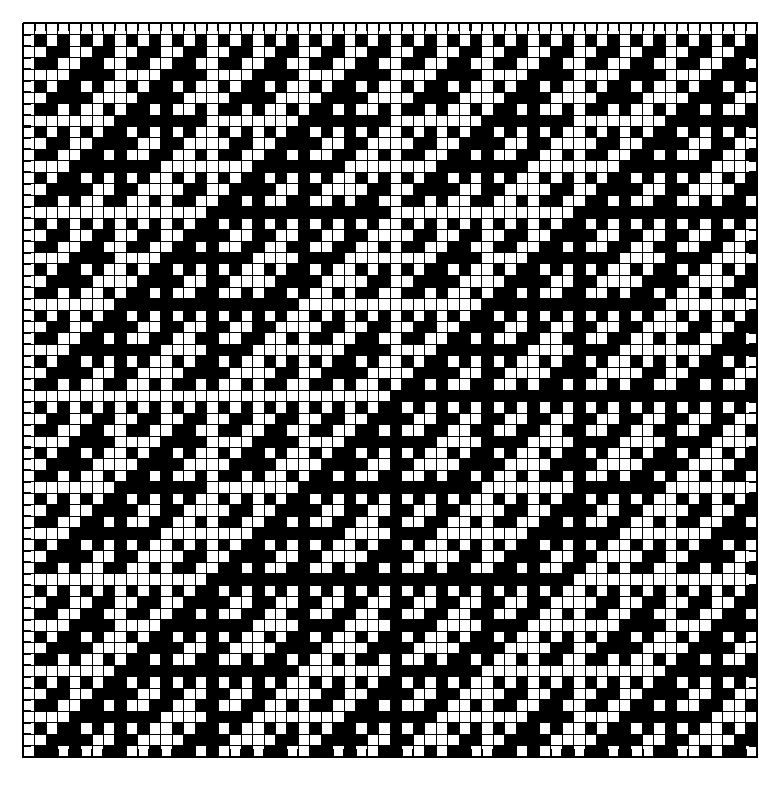
\includegraphics [scale = 0.4]{images/matrices-walsh.eps}
    \end{center}
    \caption{Walsh matrix $ W_{64} $}
              \label{fig-matrices-walsh}
\end{figure}
\end{exmp}
We can then define the \textit{Walsh transform}.
 
\begin{defn}[Walsh transform]
\index{Walsh transform} \label{notation-33} We define the \textit{Walsh transform} $ \Ww_k (f) $ of a complex vector $ f = \{f [0], \ldots, \, f [2^k-1]\} $ of size $ 2^k $ by
\begin{equation}
\label{eq-formula-defn-trans-walsh}
\forall i \in \{0, \ldots, \, 2^k-1\}, \quad \Ww_k (f) [i] \eqdef \sum_{j = 0}^{2^k-1}{f [j] \chi_i (j)} = 2^k \dotp{f}{\chi_i}.
\end{equation}
\end{defn}
 
 
\begin{rem}{(\upshape \textbf{Link with the Fourier transform}).} 
We should also note $ f: (\ZZ/2 \ZZ)^k \rightarrow \CC $ the function corresponding to the vector $ f $, that is to say the vector corresponding to the decomposition of $ f $ in the basis of Dirac functions $ \{\delta_x\}_{x \in G} $. Then the computation of $ \Ww (f) $ is that of a Fourier transform, since
\begin{equation*}
\Ww (f) [i] = 2^k \dotp{f}{\chi_i} = \wh{f} (\chi_i),
\end{equation*}
where we have denoted $ \wh{f}: \wh{G} \rightarrow \CC $ the Fourier transform of $ f $. In particular, we will therefore be able to state without effort the inversion formula for the Walsh transform.
\end{rem}
If we represent the frequencies $ i \in \{0, \ldots, \, 2^n-1\} $ on the boolean cube of the figure \figref{fig-cube-booleen}, then the frequencies located in bottom of the diagram are often referred to as \textit{low frequencies}. We find many analogies with the Fourier spectra already encountered (Fourier transforms on a finite group, continuous transform, etc.). Thus, the exercise \oldref{exo-learning-boolean-functions} proposes to use the spectral properties of the Walsh transform to perform boolean predictions (this is related to the \textit{theory of learning}) .
 
 
The operator $ \Ww_k: \CC^{2^k} \rightarrow \CC^{2^k} $ is a linear map whose matrix in the canonical basis is $ W_{2^k} $, the table of characters in the group $ (\ZZ/2 \ZZ)^k $. We thus have $ \Ww_k (f) = W_{2^k} f $. The inversion formula obtained from the proposition \ref{prop-decomposition-serie-fourier}, gives us the following information.
 
\begin{prop}
\label{prop-pte-matrix-hadamard}
\index{Inversion formula} The Walsh transform is invertible, and its inverse is $ \frac{1}{2^k} \Ww_k $. From a matrix point of view, this means that the matrix $ W_{2^k} = \{w_{ij}\} $, defined by $ w_{ij} = (-1)^{\dotp{i}{j}} $, check $ W_{2^k} W_{2^k} = 2^k Id $.
\end{prop}
The Walsh matrix makes it possible to study concrete problems, for example in statistics, as shown by the exercise \oldref{exo-transforme-walsh-statistic}.

% ------------------------------------------------- -----
% ------------------------------------------------- -----
% sub-section - Fast calculation algorithm                            
% ------------------------------------------------- -----
% ------------------------------------------------- -----
\subsection{Fast calculation algorithm}
\label{sect2-fwt} 
 
 
\index{Divide and conquer} One of the advantages of the Walsh transform is that we have a fast algorithm to calculate it. Indeed, although the equation that defines it may seem a bit complicated, it can be broken down in a simple way. This will make it possible to implement a recursive calculation algorithm, much more efficient than the naive evaluation of the sum which defines the transform. We will study in the next chapter the construction of \textit{the FFT algorithm}, and we will find exactly the same ideas, which are at the base of the algorithmic \guill{philosophy} called \textit{divide and conquer}.
 
 
\index{Algorithm!FWT} Rather than spending time on the analysis of such an algorithm (its cost, its implementation, etc.), we will simply describe the recurrence equation that we will put into{\oe } work. Discussions on the efficiency of such an implementation are postponed to the next chapter, about \textit{the FFT algorithm}. Here is the famous idea which is the basis of our algorithm. We need to rewrite the equation \eqref{eq-formula-defn-trans-walsh}, as follows:
\begin{equation*}
\Ww_k (f) [i] = \sum_{j = 0}^{2^{k-1} -1}{f [j] (-1)^{\sum_{p = 0}^{k- 2}{j_p i_p}}} + (-1)^{i_{k-1}} \sum_{j = 0}^{2^{k-1} -1}{f [j + 2^{k -1}] (-1)^{\sum_{p = 0}^{k-2}{j_p i_p}}}.
\end{equation*}
To write this expression in a simpler way, we introduce the vectors $ f_1 $ and $ f_2 $ of length $ 2^{k-1} $ defined as follows:
\begin{equation*}
\forall j \in \{0, \ldots, \, 2^{k-1} -1\}, \quad f_1 [j] = f [j] \quad \text{and} \quad f_2 [j] = f [j + 2^{k-1}].
\end{equation*}
Similarly, we will write $ \Ww_k (f)_1 $ (respectively $ \Ww_k (f)_2 $) to denote the $ 2^{k-1} $ prime (respectively last) indices of the transformed vector $ \Ww_k (f) $. We then have the recurrence equation
\begin{equation*}
\begin{split}
\Ww_k (f)_1 & = \Ww_{k-1} (f_1) + \Ww_{k-1} (f_2) \\
\Ww_k (f)_2 & = \Ww_{k-1} (f_1) - \Ww_{k-1} (f_2).
\end{split}
\end{equation*}
From a matrix point of view this decomposition is written in the form
\begin{equation*}
W_{2^k} = \begin{pmatrix} W_{2^{k-1}} & W_{2^{k-1}} \\W_{2^{k-1}} & -W_{2^{k-1}} \end{pmatrix}.
\end{equation*}
\index{Tensor product} The decomposition of $ W_{2^k} $ found corresponds to a tensor product structure, as specified in the exercise \oldref{exo-tensor-product}. \index{Matlab@\Matlab{}} This decomposition quite naturally gives rise to a very fast calculation algorithm, named \textit{FWT} for \textbf{F} ast \textbf{W} alsh \textbf{T} ransform. More precisely, if we count the number of additions necessary to calculate the Walsh transform of a vector of size $ n = 2^k $, we see that we obtain $ k = \log_2 (n ) $ recursive calls, with each time $ n $ additions or subtractions. Hence a cost of $ n \log_2 (n) $ operations. This is a substantial gain over the naive implementation of the \eqref{eq-formula-defn-trans-walsh} equation, which requires $ n^2 $ operations. The \listingterme{} \Matlab{} of this algorithm is presented in paragraph \annexeref{sect1-listing-fwt}.

% ------------------------------------------------- -----
% ------------------------------------------------- -----
% sub-section - Using the Walsh transform                            
% ------------------------------------------------- -----
% ------------------------------------------------- -----
\subsection{Use of the Walsh transform}
\label{sect2-use-fwt} 
 
 
\index{Base!orthogonal} The main interest of the Walsh transform is that it allows to decompose any function from $ \{0, \ldots, \, 2^k-1\} $ into $ \CC $ on the orthogonal basis of the characters of $ (\FF_2)^k $. More precisely, we have
\begin{equation*}
\forall i \in \{0, \ldots, \, 2^k-1\}, \quad f [i] = \frac{1}{2^k} \sum_{j = 0}^{2^{k-1}}{\Ww_k (f) [j] \chi_j (i)}.
\end{equation*}
This transform is very quick to use, because it only uses addition and subtraction (no multiplication). In addition, we have seen that we have a formidably efficient algorithm for recursively calculating the Walsh transform . However, the Walsh transform has a weak point of size: it has no pleasant property with respect to the convolution of the functions of $ \{0, \ldots, \, 2^k-1\} $ in $ \CC $, unlike the Fourier transform, as we saw in paragraph~\ref{sect2-convolution-transforme-fourier}. Indeed, the Walsh transform is a Fourier transform on the binary cube $ (\ZZ/2 \ZZ)^k $, not at all on the cyclic group $ \ZZ/2^k \ZZ $. It is mainly because of this that we will be led in the next chapter to study more closely the Fourier transform on a cyclic group. This will allow us to build an algorithm to compute convolutions on $ \ZZ/2^k \ZZ $ extremely fast.
 
 
\index{Compression} The exercise \oldref{exo-compression-walsh} shows how we can use the Walsh transform to achieve \textit{signal compression}. He also proposes to extend the Walsh transform to the two-dimensional frame.
 
 
\index{Function!boolean} \index{Non-linearity} Finally, the Walsh transform allows us to study \textit{boolean functions}, and in particular their \textit{non-linearity}. As this study supposes to consider functions with values in the finite-field $ \FF_2 $, it is approached only at the end of the chapter \oldref{chap-extension-finite-field-values}, at exercise \oldref{exo-boolean-functions}. In the same vein, the exercise \oldref{exo-learning-boolean-functions} introduces probabilistic notions to study Boolean functions and their learning.
% ------------------------------------------------- -----
% ------------------------------------------------- -----
% ------------------------------------------------- -----
% section - Poisson formula                            
% ------------------------------------------------- -----
% ------------------------------------------------- -----
% ------------------------------------------------- -----
\section{Poisson formula}
% \addcontentsline{toc}{section}{Poisson formula}
\label{sect1-fish-formula} 
 
\index{Identity!of MacWilliams} \index{MacWilliams@\nompropreindex{MacWilliams}} We have seen, in particular in Paragraph~\ref{sect2-bidual} devoted to bidual, the great similarity between duality on a finite abelian group, and duality on a vector space. In this paragraph, we will give another embodiment of this fact, in this case by studying the notion of orthogonality between a group and its dual. The central point of this approach is the \textit{Poisson formula}. We will thus see that if we apply this formula in the case of a group which is also a vector space (on a finite field), we obtain very powerful relations, called identities of \textit{MacWilliams}.
% ------------------------------------------------- -----
% ------------------------------------------------- -----
% sub-section - The formula on a finite abelian group                            
% ------------------------------------------------- -----
% ------------------------------------------------- -----
\subsection{The formula on a finite abelian group}
\label{abelian-finite-grpe-fish-formula} 
 
 
Before stating the Poisson formula on a finite group, it is necessary to clarify the notion of orthogonality. Let us start by briefly recalling the theory of orthogonality on a vector space. For a fuller description, we can refer to the work of \nompropre{Ramis}, \nompropre{Dechamps} and \nompropre{Odoux} \cite{ramis-1}.
 
 
\index{Orthogonal!of a vector space} \index{Dual!of a vector space} \label{notation-34} \label{notation-35} \label{notation-36} \index{Duality hook } If $ E $ is a finite dimensional $k$-vector space, we denote by $ E^* \eqdef \Hom (E, \, k) $ its dual, which is made up of linear forms. We classically define a bilinear form on $ E^* \times E $, which we call the hook of duality, as follows:
\begin{equation*}
\forall (f, \, x) \in E^* \times E, \quad \dotp{x}{f} \eqdef f(x).
\end{equation*}
We then define, for a part $ A \subset E $, its orthogonal
\begin{equation}
\label{eq-defn-orthogonal-ev}
A^{\bot} \eqdef \enscond{f \in E^*}{\forall x \in A, \; \dotp{x}{f} = 0}.
\end{equation}
We verify that it is a vector subspace of $ E $, and we have $ E^{\bot} = \{0\} $. Similarly, we define the orthogonal of $ B \subset E^* $ by
\begin{equation*}
B^{0} = \enscond{x \in E}{\forall f \in B, \; \dotp{x}{f} = 0}.
\end{equation*}
It is a vector subspace of $ E^* $, and we have $ (E^*)^0 = \{0\} $. Note that these properties are still true in infinite dimension, but we must use the axiom of choice. In \textit{finite} dimension, the maps $ F \mapsto F^{\bot} $ and $ G \mapsto G^0 $ are reciprocal bijections between subspaces of $ E $ and $ E^* $. They reverse inclusion.
 
 
Once in memory these linear notions of orthogonality, it is natural to introduce the following definition:
 
\begin{defn}[Orthogonal of a subgroup]
\label{defn-orthogonal-abelian-subgroup}
\index{Orthogonal!of a subgroup} \index{Subgroup} \label{notation-37} Let $ G $ be a finite abelian group, and $ H \subset G $ a subgroup. We denote by $ H^{\sharp} $ the orthogonal of $ H $ which is the subgroup of $ \wh{G} $ defined as follows:
\begin{equation*}
H^{\sharp} \eqdef \enscond{\chi \in \wh{G}}{\forall h \in H, \; \chi (h) = 1}.
\end{equation*}
\end{defn}

We have already seen during the demonstration of the lemma \ref{lem-suite-exact}, that any trivial character of $ \wh{G} $ over $ H $ is uniquely identified with an element of $ \wh{G / H} $, and vice versa. More precisely, we have an isomorphism $ H^{\sharp} \simeq \wh{G / H} $. We therefore see that $ H^{\sharp} $ is a subgroup of $ \wh{G} $ of cardinality $ |G| / | H | $. For example, we have $ G^{\sharp} = \{1\} $. In addition, the application $ H \mapsto H^{\sharp} $ reverses inclusions. Here again, the resemblance to the duality between the vector spaces is striking.
 
 
We can now state the \textit{Poisson formula} in the framework of finite abelian groups.
 
\begin{thm}[Poisson formula]
\index{Poisson's formula} \index{Poisson@\nompropreindex{Poisson}} Let $ G $ be a finite abelian group, and $ H \subset G $ a subgroup. So, for $ f: G \rightarrow \CC $, that is to say $ f \in \CC [G] $, we have
\begin{equation}
\label{eq-formula-fish-finished-grp}
\forall g \in G, \quad \sum_{h \in H}{f(gh)} = \frac{| H |}{|G|} \sum_{\chi \in H^{\sharp}}{\wh{f} (\ol{\chi}) \chi (g)}.
\end{equation}
We denote by $ \wh{f}: \wh{G} \rightarrow \CC $ the Fourier transform of $ f $.
\end{thm}

\begin{proof}
\index{Translation} To simplify the notations, we consider $ S $ a system of representatives of $ G / H $ in $ G $. We denote by $ \ol{g} $ the image of $ g \in S $ in $ G / H $ (that is to say the image by canonical projection). Let's start by defining a function $ \wt{f} $ on $ G / H $ by
\begin{equation*}
\forall g \in S, \quad \wt{f} (\ol{g}) \eqdef \sum_{h \in H}{f(gh)}.
\end{equation*}
This amounts to replacing $ f $ by an invariant function under the translation by elements of $ H $ (we \guill{periodize}). We see that this function is defined without ambiguity, since, if we consider another representative $ g'$ of the class $ g H $, we have $ g' = g h'$ with $ h' $ an element of $ H $, and therefore, $ \wt{f} (\ol{g}) = \wt{f} (\ol{g'}) $. We can therefore decompose the function $ \wt{f} \in \CC [G / H] $ into a Fourier series:
\begin{equation}
\label{eq-demo-formuel-fish-gpe-finite-tmp}
\forall g \in S, \quad \wt{f} (\ol{g}) = \sum_{\chi \in \wh{G / H}}{\dotp{\wt{f}}{\chi } \chi (\ol{g})}.
\end{equation}
We can then explain the value of the Fourier coefficients:
\begin{equation}
\label{eq-formula-fish-intermediate-result}
\dotp{\wt{f}}{\chi} = \frac{1}{| G / H |} \sum_{g \in S}{\wt{f} (\ol{g}) \ol{\chi (\ol{g})}} = \frac{| H |}{|G|} \sum_{g \in S}{\sum_{h \in H}{f(gh) \ol{\chi (\ol{g})}}}.
\end{equation}
Noticing that the application
\begin{equation*}
\func{S \times H}{G}{(g, \, h)}{gh}
\end{equation*}
is a bijection and using the fact that for $ \chi \in \wh{G / H} $, $ \chi (\ol{gh}) = \chi (\ol{g}) $, we can rewrite the sum \eqref{eq-formula-fish-intermediate-result} in the form
\begin{equation*}
\dotp{\wt{f}}{\chi} = \frac{| H |}{|G|} \sum_{g \in G}{f(g) \ol{\chi (g)}} \eqdef \frac{| H |}{|G|} \wh{f} (\ol{\chi}).
\end{equation*}
All that remains is to report the value of these coefficients in the equation \eqref{eq-demo-formuel-fish-gpe-finite-tmp} and notice that the expression of $ \wt{f} (\ol{g}) $ gives us the left side of the Poisson formula.
\end{proof}
By applying the equation \eqref{eq-formula-fish-finished-grp} with $ g = 1 $, we obtain the form in which the formula is often written:
\begin{equation}
\label{eq-formula-fish-group-finite-simple}
\sum_{h \in H}{f(h)} = \frac{| H |}{|G|} \sum_{\chi \in H^{\sharp}}{\wh{f} (\chi )}.
\end{equation}
In order to better understand the Poisson formula, we will give another proof, which uses only linear algebra arguments on the vector space $ \CC [G] $. Before giving this proof, let us study more precisely the space $ \CC [G / H] $.
 
If we denote by $ \pi: G \rightarrow G / H $ the canonical projection, we can define an application
\begin{equation*}
\pi^*: \func{\CC [G / H]}{\CC [G]}{f}{f \circ \pi}.
\end{equation*}
$ \pi^* $ is in fact an injective linear map (because $ \pi $ is surjective). The space $ \CC [G / H] $ is therefore identified with a vector subspace of $ \CC [G] $, which is in fact formed by constant functions on each of the classes on the left modulo $ H $. To demonstrate this fact, it suffices to note that $ \pi^* $ can be inverted on its image as follows:
\begin{equation*}
(\pi^*)^{-1} \func{\Im (\pi^*)}{\CC [G / H]}{f}{\wt{f}},
\end{equation*}
where we denote by $ \wt{f} (\ol{x}) $ (for $ x \in G $) the value of $ f $ on the class to the left of $ x $ modulo $ H $. This identification being made, we can give a new proof of the Poisson formula.
 
 
\begin{proof}
As before, we fix a function $ f \in \CC [G] $. Recall that the space $ \CC [G] $ is endowed with an algebra structure thanks to the convolution product $ * $, whose expression is given to the equation \eqref{eq-formula-prod-convol-grpe-abelien}. We can then consider a filtering operator
\begin{equation*}
\Phi^f: \func{\CC [G]}{\CC [G]}{\varphi}{f * \varphi}.
\end{equation*}
We will see in the Section~\ref{sect1-filtering}, why we call such operators filter operators. By using the identification between the functions of $ \CC [G / H] $ and the functions of $ \CC [G] $ constants on the classes on the left $ g H $, we can show that $ \CC [G / H] $ is a subspace of $ \CC [G] $ stable by $ \Phi^f $. Indeed, if we give ourselves $ \varphi $ constant on the classes on the left, and $ g'= g h' $, for $ g \in G $ and $ h'\in G $, we obtain
\begin{equation*}
\Phi^f(\varphi) (g') = \sum_{x \in G}{f(gh' x^{-1}) \varphi (x)} = \sum_{x \in G}{f(g (xh'^{-1})^{-1}) \varphi (x h'^{-1})} = \Phi^f(\varphi) (g).
\end{equation*}
This being shown, we can therefore consider $ \wt{\Phi}^f $, the restriction of $ \Phi^f $ to $ \CC [G / H] $. The trick to finding the Poisson formula is to calculate the trace of $ \wt{\Phi}^f $. We have an obvious basis of $ \CC [G / H] $, namely $ \Bb \eqdef \{\delta_g\}_{g \in S} $ (we always denote $ S $ a system of representative of $ G / H $). We recall that $ \delta_g $ is the function which is worth $ 1 $ in $ g $, and $ 0 $ everywhere else. In this base, the expression of the operator trace is simple to calculate, since the calculation of the images of the base vectors gives
\begin{equation*}
\forall s \in S, \quad \wt{\Phi}^f(\delta_s): g \mapsto \sum_{x \in S}{\sum_{h \in H}{f(gx^{- 1 } h^{-1}) \delta_s (x)}},
\end{equation*}
because we must remember that $ \delta_s $ is seen as a constant function on the classes on the left. As a result, we get
\begin{equation*}
\forall s \in S, \quad \wt{\Phi}^f(\delta_s): g \mapsto \sum_{h \in H}{f(gs^{-1} h^{-1})} .
\end{equation*}
The trace is therefore calculated effortlessly:
\begin{equation*}
\Tr \left(\wt{\Phi}^f \right) = \sum_{s \in S}{\sum_{h \in H}{f(ss^{-1} h^{-1}) }} = \frac{|G|}{| H |} \sum_{h \in H}{f(h)}.
\end{equation*}
Up to a constant, we get the left side of the Poisson formula. To obtain the right-hand side, it will suffice to calculate the trace of $ \wt{\Phi}^f $ in another base. And of course, we are going to reinvest the work done in the previous chapter by choosing the orthonormal basis of the characters of $ G / H $, that is to say the elements of $ H^{\sharp} $. The advantage is that the characters behave in a particularly pleasant way vis-à-vis the convolution. Indeed, the convolution theorem \ref{thm-convolution-trans-fourier-grpe-abelien}, allows to show that the elements of $ H^\sharp $ are the eigenvectors of the operator $ \wt{\Phi }^f $, since
\begin{equation*}
\forall \chi \in \wh{G / H} = H^{\sharp}, \quad \wt{\Phi}^f(\chi) = \wh{f} (\chi) \chi.
\end{equation*}
The exercise \oldref{exo-determinant-circulating}, question 1, details the proof of this. It only remains to exploit the fact that the trace of the operator $ \wt{\Phi}^f $ is equal to the sum of its eigenvalues, to conclude that
\begin{equation*}
\Tr \left(\wt{\Phi}^f \right) = \sum_{\chi \in H^{\sharp}}{\wh{f} (\chi)}.
\end{equation*}
We therefore find the simplified Poisson formula \eqref{eq-formula-fish-group-finite-simple}. To obtain the complete equation \eqref{eq-formula-fish-finished-grp}, it suffices to apply the obtained equation to the function $ f_g: x \rightarrow f(gx) $, for $ g \in G $, since we have
\begin{equation*}
\forall \chi \in \wh{G}, \quad \wh{f_g} (\chi) = \chi (g^{-1}) \wh{f} (\chi).
\end{equation*}
This reasoning shows moreover that the equations \eqref{eq-formula-fish-group-finite-simple} and \eqref{eq-formula-fish-finished-grp} are completely equivalent.
\end{proof}
 
% ------------------------------------------------- -----
% ------------------------------------------------- -----
% sub-section - Application to MacWilliams identities                            
% ------------------------------------------------- -----
% ------------------------------------------------- -----
\subsection{Application to MacWilliams identities}
\label{sect2-application-id-mac-williams} 
 
 
In this paragraph, we will use the Poisson formula as part of the group $ G $ equal to $ (\ZZ/2 \ZZ)^k = (\FF_2)^k $. We are therefore going to place ourselves in the framework where we carried out the study of the Walsh transform (Section~\ref{sect1-transforme-walsh}), and we will use the same notations. The interest of such a group is that it is in addition a vector space, in this case on the finite field $ \FF_2 $. In reality, the situation is very simple, since the notion of subgroup coincides with that of vector subspace (the group operation corresponds to the addition of vectors, and since the field has only two elements, the multiplication of a vector by a scalar is an operation which trivially respects the subgroup structure). We therefore do not lose information by translating the statements resulting from duality over a group (Poisson's formula) into the language of linear algebra. We will see that in this framework, the notions of duality and orthogonality are the same for the two structures.
 
 
All the study made in this paragraph generalizes without modification to the case of the vector space $ K^k $, where $ K $ is any finite field. The exercise \oldref{exo-generalization-mac-williams} takes this construction step by step. However, to stay within the framework developed for the Walsh transform, we will restrict ourselves to the case of the space $ (\FF_2)^k $.
 
 
Remember that we have a complete description of the dual $ \wh{F_2^k} $, since at each element $ a = \{a_0, \ldots, \, a_{k-1}\} \in ( \ZZ/2 \ZZ)^k $ we match a character
\begin{equation*}
\chi_a: \func{(\ZZ/2 \ZZ)^k}{\{- 1, \, 1\}}{x = \{x_0, \ldots, \, x_{k-1}\}}{(-1)^{\dotp{a}{x}}}.
\end{equation*}
This allows us to calculate, for a group $ H \subset G $, the orthogonal $ H^{\sharp} $. Indeed, to say that $ \chi_a \in H^{\sharp} $ is equivalent to
\begin{equation*}
\forall h \in H, \quad \chi_a (h) = (-1)^{\dotp{a}{h}} = 1.
\end{equation*}
This therefore means that
\begin{equation}
\label{eq-equivalence-orthogonalite-caractere}
\forall h \in H, \quad \dotp{a}{h} = 0 \Leftrightarrow a \in H^{\bot},
\end{equation}
where we have denoted $ H^{\bot} $ the orthogonal of $ H $ when we consider $ H $ as a vector subspace of $ (\FF_2)^k $. This orthogonal can of course be seen as the orthogonal for the canonical symmetric bilinear form on $ (\FF_2)^k $. We can also see it as the orthogonal in the sense of duality (definition \eqref{eq-defn-orthogonal-ev}), if we have identified the vector space $ (\FF_2)^k $ and its dual by identifying the canonical base with its dual base. However, be careful that the orthogonal space $ H^\bot $ has no reason to be an additional of $ H $, for example, in $ (\FF_2)^4 $, the vector $ ( 1, \, 1, \, 1, \, 1) $ is orthogonal to itself. The exercise \oldref{exo-codes-autoduaux} precisely studies the cases where the space $ H $ coincides with its dual (it uses the language of error correcting codes and group actions).
 
 
In the end, if we identify the elements $ a \in G $ and $ \chi_a \in \wh{G} $, we obtain the remarkable property that $ H^{\sharp} = H^{\bot} $ . We can now state the Poisson formula in terms of vector spaces.
 
\begin{prop}[Vector Poisson formula]
\label{prop-formula-vector-fish}
\index{Vector Poisson's Formula} Let $ H $ be a vector subspace of $ (\FF_2)^k $. Let $ f $ be a function $ f: (\FF_2)^k \rightarrow \CC $. We then have the two relations
\begin{align}
\label{eq-formula-fish-vector-1}
\sum_{a \in H}{f(a)} & = \frac{| H |}{2^k} \sum_{u \in H^{\sharp}}{\wh{f} (\chi_u )}. \\
\label{eq-formula-vector-fish-2}
\sum_{a \in H^{\sharp}}{f(a)} & = \frac{1}{| H |} \sum_{u \in H}{\wh{f} (\chi_u)} .
\end{align}
Remember that
\begin{equation*}
\wh{f} (\chi_u) \eqdef \sum_{x \in (\FF_2)^k}{(-1)^{\dotp{u}{x}} f(x)}.
\end{equation*}
\end{prop}
\begin{proof}
The first equation is the exact translation of the Poisson formula, with the identification $ H^{\bot} = H^{\sharp} $ that we have updated. For the second equation, it suffices to replace in the first $ H $ by its orthogonal $ H^{\bot} $. Like $ | H^{\bot} | = \frac{| (\FF_2)^k |}{| H |} $, we get the desired result.
\end{proof}
 
 
 
We will now be able to apply the Poisson formula for combinatorial purposes. The goal of this study is to better understand the structure of the space $ (\FF_2)^k $ when it is provided with a somewhat particular distance, which we call the distance of \textit{Hamming}. For now, it is above all a computational exercise, which will reveal some rather spectacular relationships. However, we will see in Section~\ref{sect1-applications-correctors-codes}, that all of this has applications in the study of binary corrective codes. But let us content ourselves, first of all, with defining this famous distance.
 
\begin{defn}[Hamming distance]
\index{Distance!from Hamming} \label{notation-38} \label{notation-39} Let $ x $ and $ y \in (\FF_2)^k $. We define the \textit{Hamming distance} $ d (x, \, y) $ between these two vectors as follows:
\begin{equation*}
d (x, \, y) \eqdef w (xy) \quad \text{with} \quad w (z) = \sharp \enscond{i = 0, \ldots, \, k-1}{z_i \neq 0}.
\end{equation*}
We call $ w (z) $ the weight of the vector $ z $.
\end{defn}
 
 
 
The figure \figref{fig-cube-booleen} represents the group $ (\FF_2)^4 $ where we have connected the elements at a distance of 1. In order to study the structure of a subspace $ H $ with respect to the distance $ d $, we are interested in the weight distribution of the words that form $ H $. The following definitions are then introduced.
 
\begin{defn}[Enumerator polynomial]
\index{Polynomial!enumerator} \label{notation-40} Let $ H $ be a vector subspace of $ (\FF_2)^k $. We denote by $ A_H \in \ZZ [X, \, Y] $ the \textit{enumerator polynomial of weight} of $ H $, which is defined by
\begin{equation*}
A_H (X, \, Y) \eqdef \sum_{c \in H}{X^{kw (c)} Y^{w (c)}} = \sum_{i = 0}^{k}{A_i X^{ki} Y^i},
\end{equation*}
where we denote by $ A_i $ the number of vectors of $ H $ of weight $ i $.
\end{defn}
The following relation, discovered by \nompropre{MacWilliams}, relates the weights of the words in the space $ H $ with the weights of the words of its orthogonal.
 
\begin{thm}[MacWilliams identity]
\label{thm-id-mac-williams}
\index{Identity!of MacWilliams} \index{MacWilliams@\nompropreindex{MacWilliams}} Let $ H $ be a vector subspace of $ (\FF_2)^k $. We then have
\begin{equation*}
A_{H^{\bot}} (X, \, Y) = \frac{1}{| H |} A_{H} (X + Y, \, XY).
\end{equation*}
\end{thm}
\begin{proof}
Let $ x $ and $ y $ be two fixed complex numbers. We then define the function $ f \in \CC [(\FF_2)^k] $ by
\begin{equation*}
\forall a \in (\FF_2)^k, \quad f(a) \eqdef x^{kw (a)} y^{w (a)}.
\end{equation*}
In order to apply the Poisson formula, we need to calculate $ \wh{f} $:
\begin{equation*}
\forall a \in (\FF_2)^k, \quad \wh{f} (\chi_a) \eqdef \sum_{t \in (\FF_2)^k}{x^{kw (t)} y^{w (t)} (-1)^{\dotp{t}{a}}}.
\end{equation*}
Using the fact that $ w (t) = \sum_{i = 0}^{k-1}{t_i} $ in $ \NN $, where $ t_i \in \{0, \, 1\} $, we obtain
\begin{equation*}
\forall a \in (\FF_2)^k, \quad \wh{f} (\chi_a) = \sum_{t \in (\FF_2)^k}{\prod_{i = 0}^{k-1 }{x^{1-t_i} y^{t_i} (- 1)^{a_i t_i}}} = \prod_{i = 0}^{k-1}{\sum_{t_i = 0}^1{x^{k-t_i} y^{t_i} (-1)^{a_i t_i}}}.
\end{equation*}
If $ a_i = 0 $, the inner sum is worth $ x + y $, while if $ a_i = 1 $, we find $ xy $. So we have
\begin{equation*}
\forall a \in (\FF_2)^k, \quad \wh{f} (\chi_a) = (x + y)^{kw (a)} (xy)^{w (a)}.
\end{equation*}
We can now apply the Poisson formula \eqref{eq-formula-vector-fish-2}. The equality of the theorem is thus true if we consider the values of the polynomials whatever the point $ (x, \, y) \in \CC^2 $. It is therefore also true as a polynomial equality over $ \ZZ [X, \, Y] $.
\end{proof}
 
 
 
This identity, in addition to its certain aesthetic interest, constitutes the main tool for the combinatorial study of corrective codes. The Section~\ref{sect1-codes-correctors-duality}, reformulates the identity of MacWilliams within the framework of code theory, and explains the multiple applications which result from it.

% ------------------------------------------------- -----
% ------------------------------------------------- -----
% sub-section - The Poisson formula continues                            
% ------------------------------------------------- -----
% ------------------------------------------------- -----
\subsection{The continuous Poisson formula}
 
 
\index{Poisson's formula!continuous} The Poisson formula we just used on a finite abelian group actually has a similar statement in the context of continuous functions defined on $ \RR $. To make this statement pleasant, we will define the continuous Fourier transform as follows:
\begin{equation}
\label{eq-defn-trans-fourier-special-fish}
\forall f \in L^1 (\RR), \forall x \in \RR, \quad \wh{f} (x) \eqdef \int_{\RR}{f(t) e^{- 2 \imath \pi tx} \d t}.
\end{equation}
We can then state the Poisson formula on $ \RR $. It will be noted with great interest that its proof is largely similar to that made in the framework of finite groups. The only difficulty of the continuous case lies in the problems of convergence of the manipulated series, which obliges us to impose more restrictive assumptions on the functions that we analyze.
 
\begin{thm}[Continuous Poisson formula]
\label{thm-formula-fish-continue}
Let $ f \in L^1 (\RR) $ be a continuous function such that
\begin{align}
\label{eq-formula-fish-hyp1}
& \exists M> 0, \; \exists \alpha> 1, \quad | f(x) | \leq M (1+ | x |)^{- \alpha}, \\
\label{eq-formula-fish-hyp2}
& \sum_{n = \minf}^{\pinf}{| \wh{f} (n) |} <+ \infty.
\end{align}
Under these assumptions, we have
\begin{equation}
\label{eq-formula-fish-continue}
\sum_{n = \minf}^{\pinf}{f(n)} = \sum_{n = \minf}^{\pinf}{\wh{f} (n)}.
\end{equation}
\end{thm}
\begin{proof}
\index{Series!of Fourier} \index{Periodization} We start by periodizing the function $ f $ by introducing the function
\begin{equation*}
\forall x \in \RR, \quad f_1 (x) \eqdef \sum_{n = \minf}^{\pinf}{f(x + n)}
\end{equation*}
If we restrict ourselves to the compact $ \{x \in \RR, \; | x | \leq A\} $, for $ A> 0 $, the hypothesis \eqref{eq-formula-fish-hyp1} allows to affirm, for $ | n | \geq 2A $,
\begin{equation*}
| f(x + n) | \leq M (1+ | x + n |)^{- \alpha} \leq M (1+ | n | -A)^{- \alpha} \leq M (1+ | n | / 2)^{-\alpha},
\end{equation*}
which defines the general term of a convergent series. We therefore conclude that on any compact, the series which defines $ f_1 $ is normally convergent, so that $ f_1 $ is continuous. Moreover, we can easily see that $ f_1 $ is 1-periodic, since
\begin{equation*}
f_1 (x + 1) = \sum_{n = \minf}^{\pinf}{f(x + n + 1)} = \sum_{n'= \minf}^{\pinf}{f(x + n')} = f_1 (x),
\end{equation*}
where we have made the change of variable $ n'= n + 1 $ (authorized by the absolute convergence of the series). We can therefore calculate its Fourier coefficients:
\begin{equation*}
\forall m \in \ZZ, \quad c_m (f_1) = \int_0^1{f_1 (t) e^{- 2 \imath m \pi t} \d t} = \sum_{n \in \ZZ}{\int_0^1{f(t + n) e^{- 2 \imath m \pi t} \d t}},
\end{equation*}
where the inversion between the sum and the integral is justified by the normal convergence of the series of general term $ f(t + n) e^{- 2 \imath m \pi t} $ for $ t \in [0 , 1] $. We can thus continue the calculations to obtain, by changing the variable $ u = t + n $,
\begin{equation*}
\forall m \in \ZZ, \quad c_m (f_1) = \sum_{n \in \ZZ}{\int_{n}^{n + 1}{f(u) e^{- 2 \imath m \pi u}} \d u} = \int_{\minf}^{\pinf}{f(u) e^{- 2 \imath m \pi u} \d u} = \wh{f} (m)
\end{equation*}
(the last equality is justified by Lebesgue's dominated convergence theorem, because $ x \mapsto f(x) e^{- 2 \imath m \pi x} \in L^1 (\RR) $). We therefore note, with the hypothesis \eqref{eq-formula-fish-hyp2} that the Fourier series associated with $ f_1 $ absolutely converges. By additionally using the fact that $ f_1 $ is a continuous function, we therefore conclude that it is the sum of its Fourier series. We can therefore write
\begin{equation*}
\forall x \in \RR, \quad f_1 (x) = \sum_{m \in \ZZ}{c_m (f_1) e^{2 \imath m \pi x}} = \sum_{m \in \ZZ }{\wh{f} (m) e^{2 \imath m \pi x}}.
\end{equation*}
In the end, we therefore obtain equality
\begin{equation*}
\forall x \in \RR, \quad \sum_{n \in \ZZ}{f(x + n)} = \sum_{m \in \ZZ}{\wh{f} (m) e^{2 \imath m \pi x}},
\end{equation*}
which gives the desired Poisson formula by making $ x = $ 0.
\end{proof}
 
 
\begin{rem}{(\upshape \textbf{Link with Poisson's formula on a finite group}).} 
\index{Quotient} \index{Group!quotient} The continuous Poisson formula that we have just demonstrated is in all points similar to the formula \eqref{eq-formula-fish-finished-grp}, valid on a finite abelian group . Indeed, in the continuous case, we must consider the group $ G = \RR^1 $, which is the real line provided with the addition, as well as the discrete subgroup $ \ZZ \subset \RR $. The quotient group is nothing other than the circle $ \RR / \ZZ \simeq S^1 $. Moreover, we will see in Paragraph~\ref{sect2-transforme-fourier-continue}, that we have a complete description of the characters of the circle, since they correspond to the exponentials $ e_n: t \mapsto e^{2 \imath n \pi t} $. We therefore have an explicit isomorphism $ \wh{S^1} \simeq \ZZ $. Therefore, we can write the Poisson formula in the continuous case in the form
\begin{equation*}
\sum_{n \in \ZZ}{f(n)} = \sum_{e_n \in \wh{\RR / \ZZ}}{\dotp{f}{e_n}}.
\end{equation*}
So up to the factor $ \frac{| H |}{|G|} $, this formula is in every way similar to \eqref{eq-formula-fish-finished-grp}.
\end{rem}
 
 
 
\index{Function!Theta of Jacobi} One of the many applications of Poisson's formula concerns the function \textit{Theta} of \textit{Jacobi}, which is defined as follows.
 
\begin{defn}[Jacobi Theta Function]
We define the function \textit{Theta} by
\begin{equation*}
\forall t> 0, \quad \theta (t) \eqdef \sum_{n = \minf}^{\pinf}{e^{- \pi n^2 t}}.
\end{equation*}
\end{defn}
Before stating the functional equation that $ \theta $ satisfies, we need to prove a classical lemma on the Fourier transform of a Gaussian.
 
\begin{lem}
\label{lem-tf-gaussienne}
\index{Gaussian} Let $ g_t $, for $ t> 0 $, be the Gaussian defined by
\begin{equation*}
\forall x \in \RR, \quad g_t (x) = e^{- \frac{x^2}{2t}}.
\end{equation*}
So we have
\begin{equation*}
\forall x \in \RR, \quad \wh{g_t} (x) = \sqrt{2 \pi t} e^{- 2 \pi^2t x^2}
\end{equation*}
where we have kept the definition of the Fourier transform \eqref{eq-defn-trans-fourier-special-fish}.
\end{lem}
\begin{proof}
The transform of the function $ g_t $ is written
\begin{equation*}
\wh{g_t} (x) = \int_{\RR}{e^{- \frac{u^2}{2t}} e^{- 2 \imath \pi ux} \d u}.
\end{equation*}
Using the derivation theorem under the sum sign, we see that the function obtained is $ C^1 $, and that we have
\begin{equation*}
\frac{\d \wh{g_t}}{\d x} (x) = -2 \imath \pi \int_{\RR}{ue^{- \frac{u^2}{2t}} e^{-2 \imath \pi ux} \d u} = -4 \pi^2 xt \wh{g_t} (x),
\end{equation*}
where the last equality is obtained by integration by parts. By solving the differential equation of which $ g_t $ is the solution, we obtain
\begin{equation*}
\wh{g_t} (x) = \wh{g_t} (0) e^{- 2 \pi^2 tx^2}.
\end{equation*}
It only remains to calculate the value of $ \wh{g_t} (0) = \sqrt{t} I $, with $ I = \int_{\RR}{e^{- x^2/2} \d x} $. To do this, it is advisable to switch to polar coordinates when calculating $ I^2 $:
\begin{equation*}
I^2 = \int_{\RR}{\int_{\RR}{e^{- \frac{x^2 + y^2}{2}} \d x} \d y} = 2 \pi \int_0^{\pinf}{re^{- \frac{r^2}{2}} \d r} = 2 \pi.
\end{equation*}
By putting all these results end to end, we get the announced Fourier transform.
\end{proof}
Here is finally the identity of Jacobi on the function $ \theta $.
 
\begin{thm}[Identity of Jacobi]
\index{Identity!of Jacobi}
\begin{equation}
\label{eq-id-jacobi}
\forall t> 0, \quad \theta (t) = \frac{1}{\sqrt{t}} \theta \left(\frac{1}{t} \right)
\end{equation}
\end{thm}
\begin{proof}
It suffices to apply Poisson's formula to the function $ g_t $. It is obvious that $ g_t $ satisfies the hypotheses of the theorem \ref{thm-formula-fish-continue}. We thus obtain the following equality:
\begin{equation*}
\sum_{n \in \ZZ}{g_t (n)} = \sum_{n \in \ZZ}{e^{- \frac{n^2}{2t}}} = \sum_{n \in \ZZ}{\wh{g_t} (n)} = \sqrt{2 \pi t} \sum_{n \in \ZZ}{e^{- 2 \pi^2 tn^2}}.
\end{equation*}
It is nothing other than the identity that we were trying to prove, evaluated in $ 2 \pi t $.
\end{proof}
\index{Matlab@\Matlab{}} One of the interests of this identity is to allow to calculate the function $ \theta $ for small values of the parameter $ t $, and this with a very high precision. For example, for $ t = 0.001 $, the right hand side of \eqref{eq-id-jacobi} instantly provides the result with a precision greater than that of \Matlab{} in double precision (which is given by the command \texttt{eps = 2.2204e-016}), and this with simply the index term $n = 0$  in the sum. If we naively use the left side of the identity, we observe a relatively slow geometric decrease in error.

% ------------------------------------------------- -----
% ------------------------------------------------- -----
% ------------------------------------------------- -----
% section - Exercises                            
% ------------------------------------------------- -----
% ------------------------------------------------- -----
% ------------------------------------------------- -----
\section{Exercises}
% \addcontentsline{toc}{section}{Exercises}
 
 
 
\begin{exo}[Geometric proof of quadratic reciprocity]
\label{exo-proof-geom-reciprocite}
 
\index{Eisenstein@\nompropreindex{Eisenstein}} \index{Quadratic reciprocity} This exercise is taken from an article by \nompropre{Laubenbacher}{\upshape{\cite{laubenbacher}}}. We will detail step by step the proof of quadratic reciprocity that \nompropre{Eisenstein} gave in 1844. This proof is quite original since it mainly uses arguments of a geometric nature. In the rest of this exercise, we denote by $ [x]_p $ the remainder of the Euclidean division of $ x $ by $ p $ (which is always an element of $ \{0, \ldots, \, p-1\} $, even if $ x \leq 0 $), and $ \lfloor x \rfloor $ the integer part of $ x $. We consider two distinct odd prime numbers $ p $ and $ r $, and we want to prove the quadratic reciprocity formula \eqref{eq-reciprocity-quadratic}. \begin{enumerate}
\item We denote by $ A \eqdef \{2, \, 4, \, 6, \ldots, \, p-1\} $ and $ B \eqdef \enscond{[ra]_p}{a \in A} $. Show that we have
\begin{equation*}
A = \enscond{\left[(-1)^bb \right]_p}{b \in B}.
\end{equation*}
 
\item Deduce that modulo $ p $, we have the following equality:
\begin{equation*}
\prod_{b \in B}{b} = r^{\frac{p-1}{2}} \prod_{a \in A}{a} = r^{\frac{p-1}{2 }} (-1)^{\sum_{b \in B}{b}} \prod_{b \in B}{b} \mod{p},
\end{equation*}
since
\begin{equation*}
\legsymb{r}{p} = (-1)^{\sum_{b \in B}{b}}.
\end{equation*}
 
\item Prove the following equality:
\begin{equation*}
\sum_{a \in A}{ra} = p \sum_{a \in A}{\left\lfloor \frac{ra}{p} \right\rfloor} + \sum_{b \in B}{b }.
\end{equation*}
To deduce
\begin{equation*}
\legsymb{r}{p} = (-1)^{\sum_{a \in A}{\left\lfloor \frac{ra}{p} \right\rfloor}}.
\end{equation*}
 
\item In order to give a geometric meaning to this equation, we construct the figure \figref{fig-demo-geom-reciprocite}. Show that no point with integer coordinates lies on $] AB [$. Show then that the number of even abscissa points in the triangle $ ABD $ is equal to $ \sum_{a \in A}{\left\lfloor \frac{ra}{p} \right\rfloor} $.
\item We consider an entire abscissa $ a> \frac{p}{2} $. Show that, modulo 2, the number of points of abscissa $ a $ located below $ (AB) $ (marked $ + $ in the figure) is equal to the number of points of the same abscissa but located above $ (AB) $ (marked $ \times $). Show that this number is also equal to the number of abscissa points $ pa $ located below $ (AB) $ (noted $ \bullet $). Conclude that $ \sum_{a \in A}{\left\lfloor \frac{ra}{p} \right\rfloor} $ is equal, modulo 2, to the number of points with integer coordinates in the interior of the triangle $ AHK $.
\item By swapping the roles of $ p $ and $ r $, then counting the points in the rectangle $ ALHK $, deduce the quadratic reciprocity law.
\end{enumerate} \begin{figure}[ht] 
    \begin{center}
    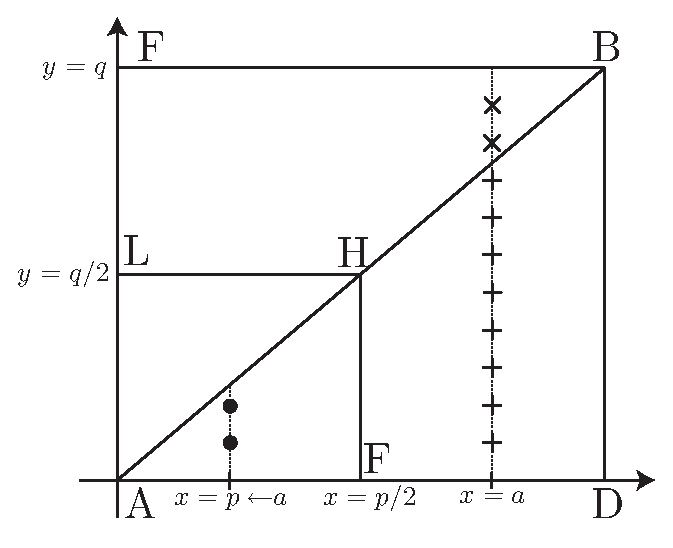
\includegraphics [scale = 0.7]{images/demo-geom-reciprocite.eps}
    \end{center}
    \caption{Geometric proof of the quadratic reciprocity law}
              \label{fig-demo-geom-reciprocite}
\end{figure}
\end{exo}
 
 
\begin{exo}[Fermat's theorem on a finite field]
\label{exo-thm-fermat-finite-body}
 
\index{Fermat's equation} \index{Fermat@\nompropreindex{Fermat}} This exercise uses the notations and results of the exercise \oldref{exo-eqn-grpe-abelien-finite}. Let $ q = p^r $ where $ p $ is a prime number. We want to show that if $ k $ is an integer such that $ q \geq k^4 + 4 $, then Fermat's equation on $ \FF_q $
\begin{equation}
\label{eq-thm-fermat-finite-body}
x^k + y^k = z^k \quad \quad \quad x, \, y, \, z \in \FF_q^*
\end{equation}
has a solution. To do this, we will use the Fourier transform on the group $ (\FF_q, \, +) $. \begin{enumerate}
\item \index{Subgroup} Let $ k | q-1 $. Show that there exists a unique subgroup $ H_k $ of index $ k $ in $ \FF_q^* $ and that
\begin{equation*}
H_k = \enscond{x^k}{x \in \FF_q^*}.
\end{equation*}
 
\item \index{Group!quotient} We denote by $ \chi_0, \ldots, \, \chi_{k-1} $ the multiplicative characters of the quotient group $ \FF_q^* / H_k $. They are canonically extended into multiplicative characters of $ \FF_q^* $ by composing by the canonical projection. Show then that for any additive character $ \psi $ we have
\begin{equation*}
\wh{f_{H_k}} (\psi) = \frac{1}{k} \sum_{i = 0}^{k-1}{G (\chi_i, \, \psi)}.
\end{equation*}
Using the proposition \ref{prop-calcul-sums-gauss}, show then that $ \Phi (H_k) <\sqrt{q} $, where $ \Phi $ is defined by the equation \eqref{eq-defn-phi-ensemble}.
\item Let $ A_1, \, A_2 \subset G $. We denote by $ N $ and $ N'$ respectively the number of solutions of the equations
\begin{align}
\label{eq-thm-fermat_intermediaire}
x + y & = z^k, \quad \quad & \text{with} \quad x \in A_1, \; y \in A_2, \; z \in \FF_q^*, \\
x + y & = u, \quad \quad & \text{with} \quad x \in A_1, \; y \in A_2, \; u \in H_k.
\end{align}
Show that $ N = k N'$, then show that
\begin{equation}
\label{eqn-fermat-majoration}
\left| N - \frac{| A_1 | | A_2 | (q-1)}{q} \right| <k \sqrt{| A_1 | | A_2 | q}.
\end{equation}
We can start by proving a similar inequality for $ N'$ using the result of the exercise \oldref{exo-eqn-grpe-abelien-finite}, question 2.
\item If we denote by $ l_i \eqdef \frac{q-1}{| A_i |} $, then show that if $ q \geq k^2 l_1 l_2 + 4 $ the equation \eqref{eq-thm-fermat_intermediaire} admits a solution. In the case where $ k $ does not divide $ q-1 $, show that
\begin{equation*}
\enscond{x^k}{x \in \FF_q^*} = \enscond{x^d}{x \in \FF_q^*},
\end{equation*}
where $ d \eqdef \PGCD (q-1, \, k) $. Deduce that the result is valid for any $ k $ satisfying $ q \geq k^2 l_1 l_2 + 4 $.
\item Using the sets $ A_1 = A_2 = H_k $, show that if $ q \geq k^4 + 4 $, then the equation \eqref{eq-thm-fermat-finite-body} admits at least one solution .
\end{enumerate}
\end{exo}
 
 
\begin{exo}[Walsh transform and statistical study]
\label{exo-transforme-walsh-statistic}
 
This exercise is taken from an article by \nompropre{Rockmore} and \nompropre{Malsen}{\upshape \cite{rockmore-generalized}}, which presents a technique known as the analysis of \textit{Yates}, from the name of the statistician who invented this method. Consider the following situation: a farmer wants to know the influence of three parameters on his wheat production. These parameters are the lighting (represented by the variable $ a $), the amount of herbicide (variable $ b $), and the amount of fertilizer (variable $ c $). Each of these variables can take two values: high quantity (noted $ + $) and low quantity (noted $ - $). An experimental report is given in the form of the following table grouping the values for the average size of wheat (in centimeters) under the different conditions:
\begin{equation*}
\begin{array}{c | c | c || c} a & b & c & \alpha_{abc} \\\hline + & + & + & 69 \\- & + & + & 81 \\+ & - & + & 63 \\- & - & + & 77 \\+ & + & - & 61 \\- & + & - & 92 \\+ & - & - & 54 \\- & - & - & 89 \end{array}
\end{equation*}
We can therefore represent these results in the form of a function
\begin{equation*}
f: \func{(\ZZ/2 \ZZ)^3 \simeq \{-, +\}^3}{\RR}{(a, \, b, \, c)}{\alpha_{abc} }.
\end{equation*}
In order to analyze these results, we define the 0-order interaction, denoted $ \mu $, which is simply the mean:
\begin{equation*}
\mu \eqdef \frac{1}{8} \sum_{(a, \, b, \, c) \in \{+, -\}^3}{\alpha_{abc}}.
\end{equation*}
We then define the interactions of order 1, denoted $ \mu_a $, $ \mu_b $ and $ \mu_c $, as corresponding to the effect of a single parameter, the other two being assumed to be constant. For example we have
\begin{equation*}
\mu_{a} \eqdef \frac{1}{4} \sum_{(b, \, c) \in \{+, -\}^2}{\alpha_{+ bc}} - \frac{1 }{4} \sum_{(b, \, c) \in \{+, -\}^2}{\alpha_{- bc}}.
\end{equation*}
In the same vein, define the 3 interactions of order 2, denoted by $ \mu_{ab} $, $ \mu_{bc} $ and $ \mu_{ac} $, as well as the interaction of order 3, denoted by $ \mu_{abc} $. How can we calculate all these interactions using the Walsh transform? Deduce a fast calculation algorithm. Do the math for the farmer.
\end{exo}
 
 
\begin{exo}[Haar wavelet]
\label{exo-wavelet-haar}
 
\index{Wavelet!of Haar} \index{Haar@\nompropreindex{Haar}} \index{Base!orthonormal} \index{Base!of Haar} \index{Base!of Hilbert} We denote $ \psi_0 $ the function indicator of $ [0, \, 1] $ and $ \psi $ the function which is worth $ 1 $ on $ [0, \, \frac{1}{2}[$, $ -1 $ on $ [\frac{1}{2}, \, 1] $, and $ 0 $ everywhere else. We then define a series of functions $ \psi_n $ by
\begin{equation*}
\forall j \geq 1, \; \forall k \in \{0, \ldots, \, 2^{j-1} -1\}, \quad \psi_n (x) \eqdef \psi_{j, k} (x) \eqdef 2^{\frac{j}{2}} \psi \left(2^jx - k \right),
\end{equation*}
where $ n = 2^{j-1} + k $. We denote, for $ j \geq 0 $, $ F_j $ the space of functions of $ [0, \, 1] $ in $ \RR $ constants on each of the intervals $ I_k \eqdef [k 2^{- j }, \, (k + 1) 2^{- j}[$, for $ k \in \{0, \ldots, \, 2^j-1\} $ (we include the point $ 1 $ in the last interval). \begin{enumerate}
\item Show that $ \left\{\psi_n \right\}_{n = 0}^{2^j-1} $ forms an orthonormal basis of $ F_j $ for the usual scalar product of $ L^2 ([ 0, \, 1]) $.
\item Let $ f $ be a continuous function of $ [0, \, 1] $ in $ \RR $. For $ J \geq 0 $, we denote by $ f_J $ the projection of $ f $ on $ F_J $:
\begin{equation*}
f_J \eqdef \sum_{j = 0}^J{\sum_{k = 0}^{2^{j-1} -1}{\dotp{f}{\psi_{j, k}} \psi_{j, k}}}.
\end{equation*}
Show that $ f_J $ converges uniformly on $ [0, \, 1] $ to $ f $ when $ J \rightarrow + \infty $. We then define, for $ n \geq 0 $, the function
\begin{equation*}
\wt{f}_n \eqdef \sum_{m = 0}^{n}{\dotp{f}{\psi_m} \psi_m}.
\end{equation*}
Show that $ \wt{f}_n $ converges uniformly to $ f $ when $ n \rightarrow \infty $. Then show that $ \{\psi_n\}_{n \in \NN} $ forms a Hilbert basis of $ L^2 ([0, \, 1]) $. The figure \figref{fig-decomposition-base-haar} represents the decomposition of a function $ f $ on the first vectors of the base of $ \psi_n $, which we call the Haar base. \begin{figure}[ht]
    \begin{center}
    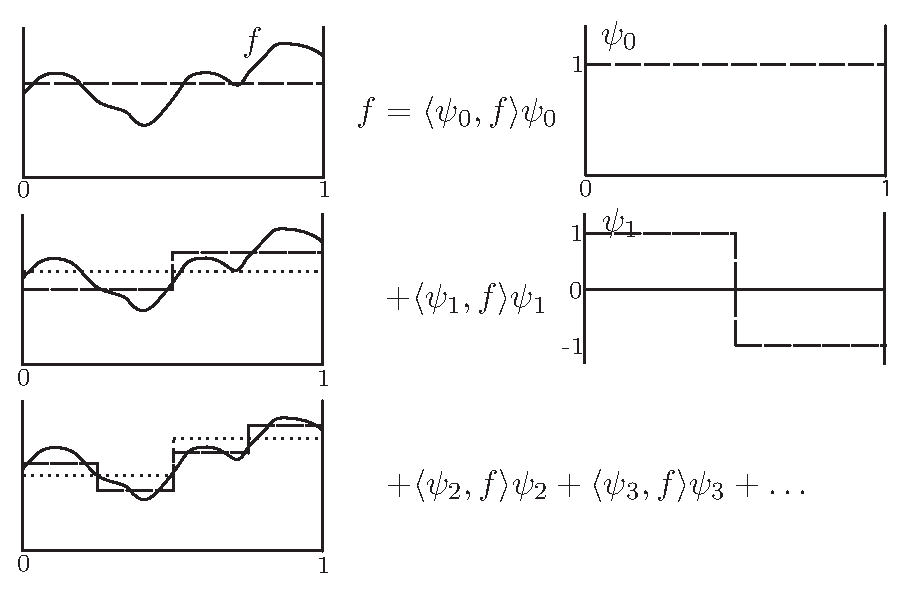
\includegraphics [scale = 0.8]{images/decomposition-base-haar.eps}
    \end{center}
    \caption{Decomposition based on Haar}
              \label{fig-decomposition-base-haar}
\end{figure}
 
\item We introduce, for $ j \geq 0 $, the functions \guill{stepped} $ \varphi_{j, k} (x) \eqdef 2^{\frac{j}{2}} \psi_0 \left(2^jx - k \right) $. Show that $ \varphi_{j, k} $, for $ k \in \{0, \ldots, \, 2^j-1\} $, forms an orthonormal basis of $ F_j $. We define $ G_{j-1} $ the vector space such that $ F_j = F_{j-1} \oplus G_{j-1} $ (space of \guill{details}). Show that $ \{\psi_{j, k}\}_{k = 0}^{2^{j-1} -1} $ is an orthonormal basis of $ G_{j-1} $. Then express the function $ \psi_{j, k} $ as a linear combination of $ \varphi_{j + 1, s} $, $ s \in \{0, \ldots, \, 2^j-1 $.
\item Let $ f \in F_j $. We denote by $ x^{(0)} \in \RR^{2^j} $ the vector of scalar products $ x^{(0)}[k] = \dotp{f}{\varphi_{j, k }} $. How do you calculate them from $ f $? For $ i \in \{1, \ldots, \, j\} $, we define vectors $ x^{(i)} $ and $ d^{(i)} $ of size $ 2^{ji} $ , by the relations, for $ k \in \{0, \ldots, \, 2^{ji} -1\} $,
\begin{align*}
x^{(i)}[k] & \eqdef \frac{x^{(i-1)}[2k + 1] + x^{(i-1)}[2k]}{\sqrt{2} } \\
d^{(i)}[k] & \eqdef \frac{x^{(i-1)}[2k + 1] - x^{(i-1)}[2k]}{\sqrt{2} }.
\end{align*}
\index{Rotation} \index{Signal} Intuitively, $ x^{(i)} $ represents the trend in the signal $ x^{(i-1)} $, and $ d^{(i)} $ represents the details. The figure \figref{fig-decomposition-wavelet-haar} symbolizes the succession of calculations to be performed to obtain the vectors $ d^{(i)} $ as well as the last coefficient $ x^{(j)}[0] $ . Show that the operator $ x^{(i)} \mapsto (x^{(i + 1)}, \, d^{(i + 1)}) $ can be seen as an isometry (more precisely a rotation ) of $ \RR^{ji} $. Show that the $ x^{(i)} $ all have the same average, and therefore that $ x^{(j)}[0] $ represents the average of the original $ x^{(0)} $ signal . 

\begin{figure}[ht]
    \begin{center}
    \includegraphics[scale=1.0]{images/decomposition-ondelette-haar.eps}
    \end{center}
    \caption{Cascade calculation of the decomposition coefficients}
              \label{fig-decomposition-wavelet-haar}
\end{figure}
 
\item Show that we have, for $ i \in \{1, \ldots, \, j\} $ and for $ k \in \{0, \ldots, \, 2^{ji} -1\} $,
\begin{equation*}
d^{(i)}[k] = \dotp{f}{\psi_{j-i + 1, k}} \quad \quad \text{and} \quad \quad x^{(j)}[ 0] = \dotp{f}{\psi_0}.
\end{equation*}
Thanks to this algorithm, what is the number of operations necessary to decompose a function of $ F_j $ on the basis of $ \psi_n $?
\item \index{Complexity} We assume that $ n = 2^j $. Show that the operator $ \Gamma $ which to $ x \in \RR^{n} $ associates the vector $ (d^{(1)}, \, x^{(2)}, \ldots, \, d^{(j)}, \, x^{(j)}) $ is an isometry of $ \RR^{n} $ for the canonical dot product (we put the vectors $ d^{( i)}, \, x^{(i)}, \ldots $). Deduce that the application of this operator corresponds to the decomposition of $ x $ in an orthonormal basis of $ \RR^{n} $ that we will specify. Compare this database to the Walsh database described in paragraph~\ref{sect2-presentation-transforme-walsh}. Compare in terms of complexity the algorithm of decomposition in the base of Haar and that of decomposition in the base of Walsh (FWT algorithm, paragraph~\ref{sect2-fwt}).
\end{enumerate} Figure \figref{fig-transforme-haar} shows two examples of transforms $ y = \Gamma x $. We can see that since the signals are regular, only the coefficients corresponding to the coarse scales (that is to say for $ j $ small, the indices on the right of the transform) are large. \begin{figure}[ht]
    \begin{center}
    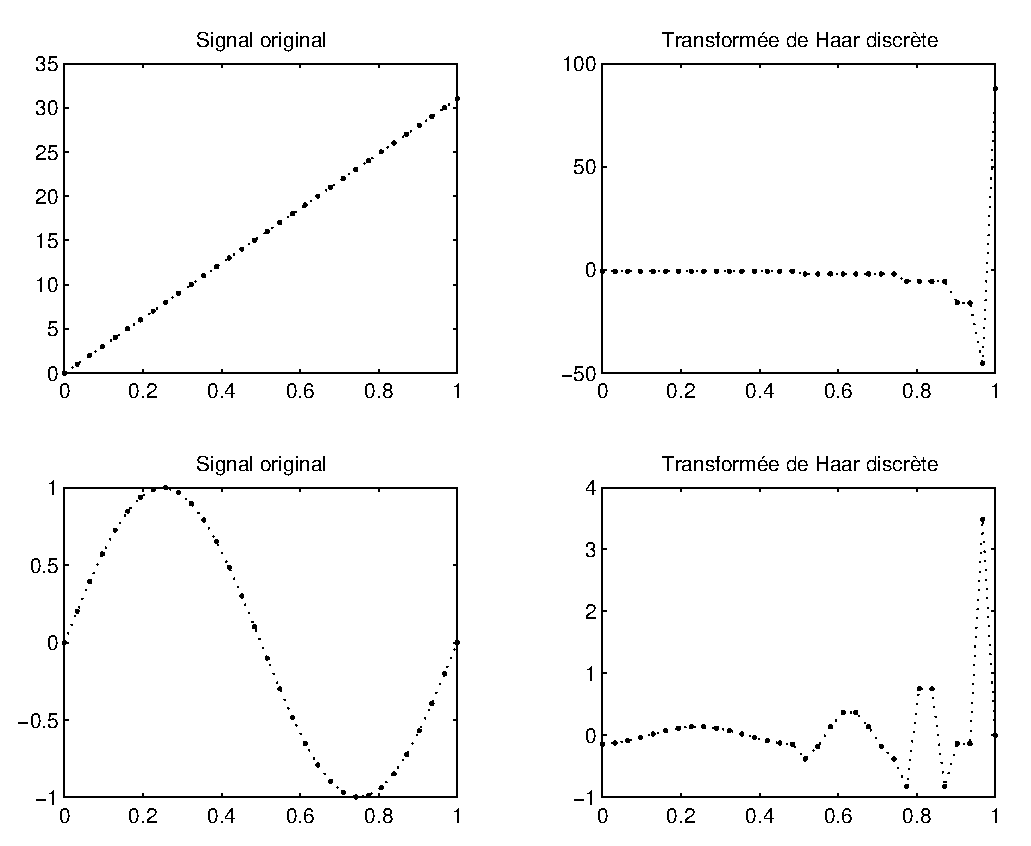
\includegraphics [scale = 0.7]{images/transformee-haar.eps}
    \end{center}
    \caption{Examples of discrete Haar transforms}
              \label{fig-transforme-haar}
\end{figure}
The Haar base is the simplest example of a wavelet base. The fast wavelet transformation algorithm was introduced by \nompropre{Mallat},{\upshape \cite{mallat}}. The differences between the Walsh and Haar bases illustrate the transition from the Fourier transform (here on $ (\FF_2)^k $) to the wavelet transform. The exercise \oldref{exo-wavelets-finite-fields} presents the construction of wavelets on finite fields.
\end{exo}
 
 
\begin{exo}[Image compression]
\label{exo-compression-walsh}
\index{Compression} The goal of this exercise is to properly order Walsh functions to successfully compress 1D and 2D signals. \begin{enumerate}
\item \index{2D Walsh transform} Generalize the discrete Walsh transform to the two-dimensional case. We will use the functions
\begin{equation*}
\chi_{i, \, j} (s, \, t) = \chi_i (s) \chi_j (t).
\end{equation*}
Write a fast computation algorithm for the 2D Walsh transform.
\item Show that we can classify the discrete Walsh functions (defined by the equation \eqref{eq-denf-base-walsh}) in increasing order of the number of sign changes. The figure \figref{fig-functions-walsh} shows the Walsh matrices obtained by classifying the functions in the usual order and in the order of the number of sign changes. \begin{figure}[ht]
    \begin{center}
    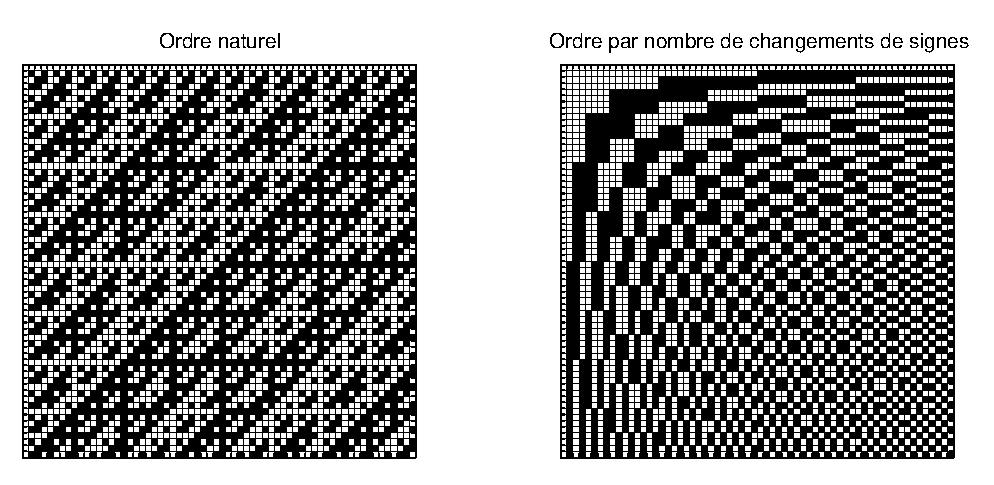
\includegraphics [scale = 0.7]{images/fonctions-walsh.eps}
    \end{center}
    \caption{Two ways to classify Walsh functions}
              \label{fig-functions-walsh}
\end{figure}
 
\item \index{Signal} Intuitively, such a classification makes it possible to order the Walsh spectrum from tendencies (low frequencies) to details (high frequencies). Calculate for some functions the spectra obtained with the two classifications, and verify this interpretation. The figure \figref{fig-spectrum-walsh-1d} shows the spectra of the function represented at the top left of the figure \figref{fig-compression-walsh-1d}. 

\begin{figure}[ht]
    \begin{center}
    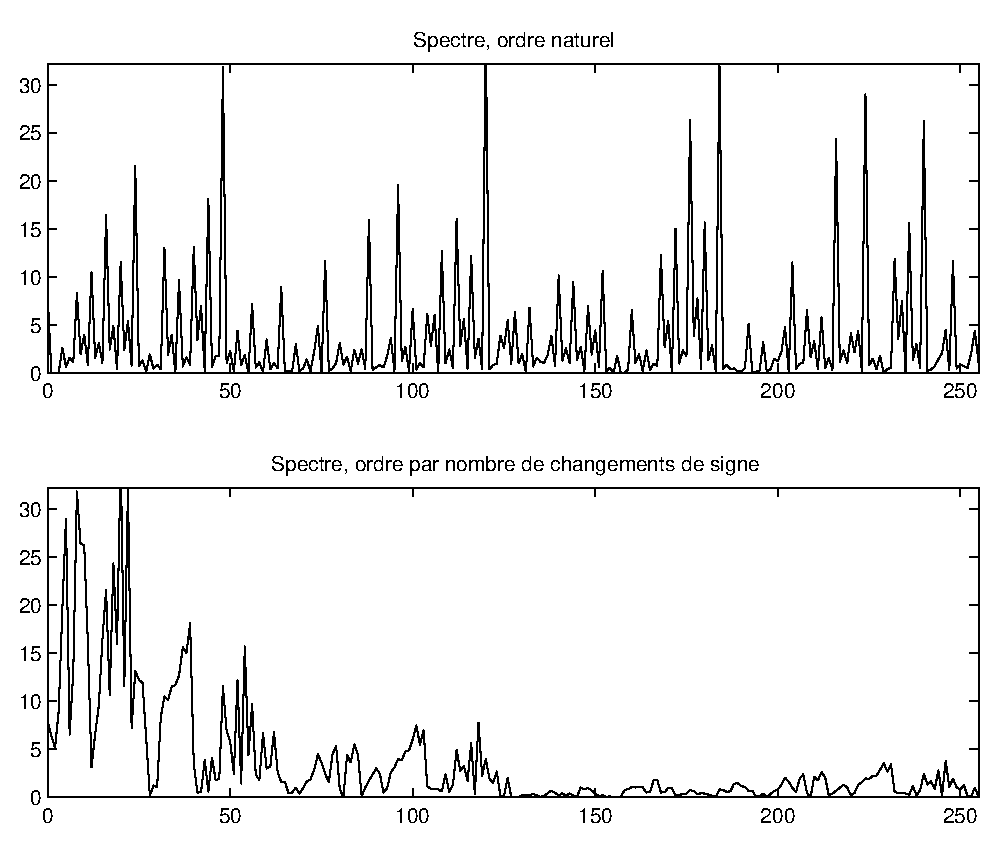
\includegraphics[scale = 0.5]{images/spectre-walsh-1d.eps}
    \end{center}
    \caption{Walsh spectrum of a 1D signal}
              \label{fig-spectrum-walsh-1d}
\end{figure}
 
\item We have therefore classified the Walsh functions according to an order $ \chi_{i_0}, \ldots, \, \chi_{i_N} $. We consider a signal $ f \in \CC^N $. For $ 0 \leq n <N $, we construct the function
\begin{equation*}
f_n \eqdef \sum_{k = 0}^{n}{\dotp{f}{\chi_{i_k}} \chi_{i_k}}.
\end{equation*}
Explain why this process allows to compress the signal $ f $. Figure \figref{fig-compression-walsh-1d} shows the progressive compression of a signal. The percentage of Walsh coefficients which have been retained is indicated each time. After studying the discrete Fourier transform in chapter \oldref{chap-tfd}, we can perform the same process, but with the Fourier spectrum. What are the advantages and disadvantages of each method (calculation time, quality of reconstruction, etc.)? \begin{figure}[ht]
    \begin{center}
    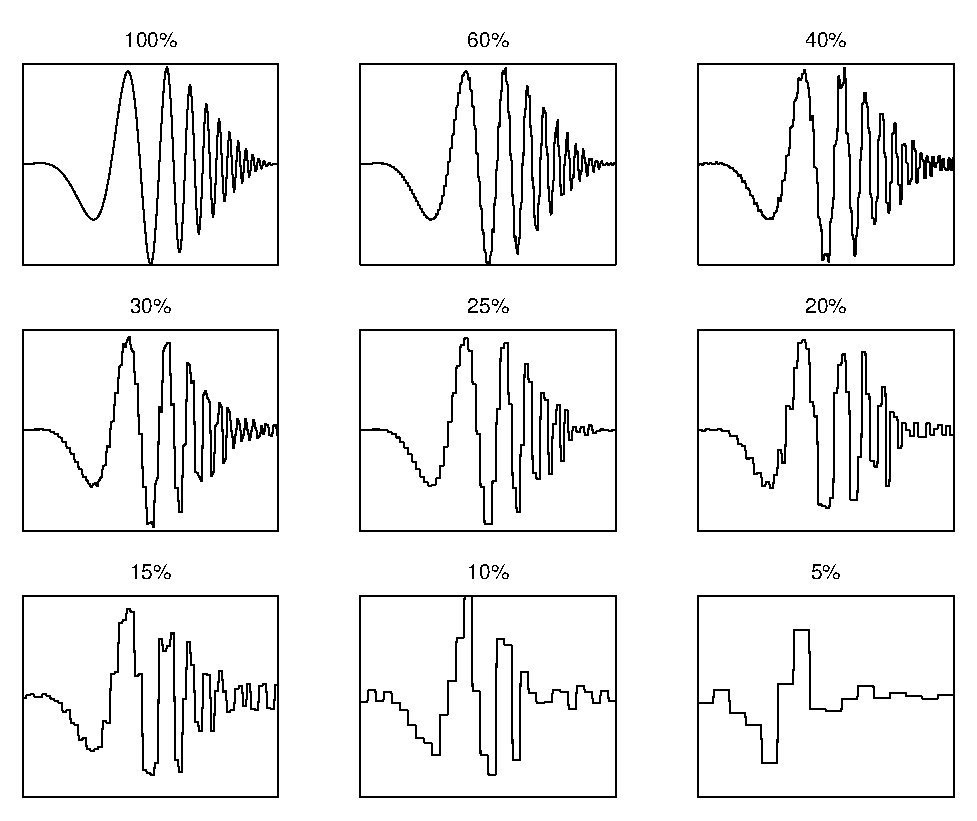
\includegraphics [scale = 0.6]{images/compression-walsh-1d.eps}
% \includegraphics [scale = 0.6]{images/compression-walsh-1d-2.eps}
    \end{center}
    \caption{Compression of a 1D signal}
              \label{fig-compression-walsh-1d}
\end{figure}
 
\item What classification (s) can we adopt for the functions of Walsh 2D? The figure \figref{fig-functions-walsh-2d} proposes such a classification (from left to right and top to bottom). \begin{figure}[ht]
    \begin{center}
    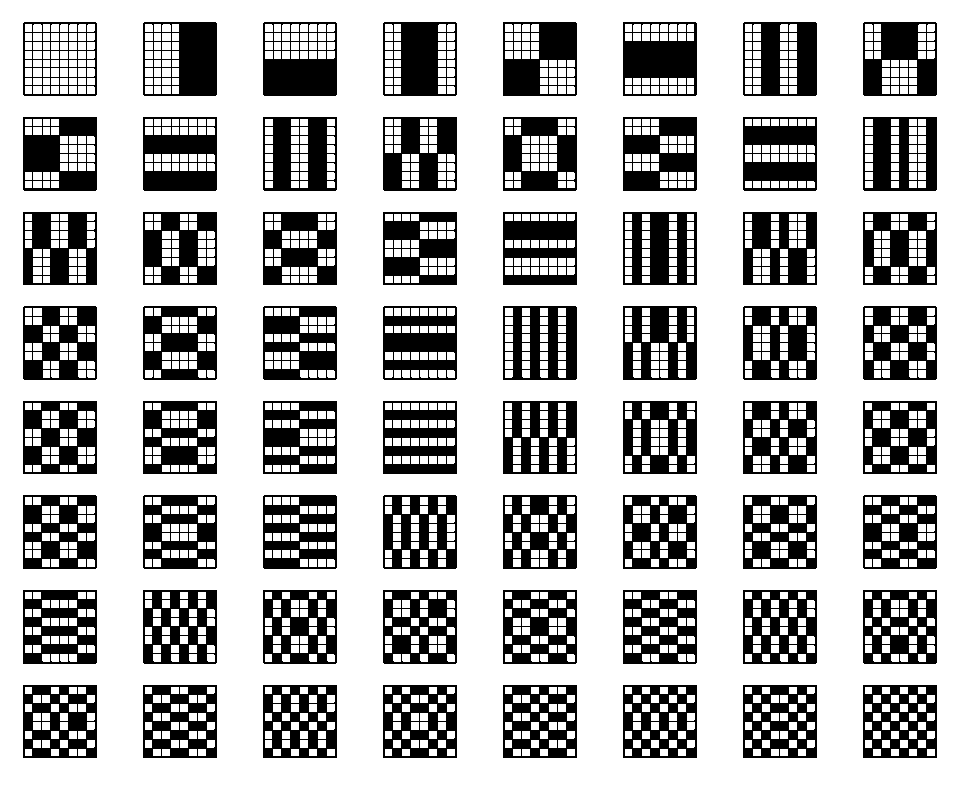
\includegraphics [scale = 0.6]{images/fonctions-walsh-2d.eps}
    \end{center}
    \caption{Classification of 2D Walsh functions}
              \label{fig-functions-walsh-2d}
\end{figure}
Apply this classification to compress 2D images. Write a \Matlab{} program to perform this compression. The figure \figref{fig-compression-walsh-2d} shows the progressive compression of an image representing the letter A. \begin{figure}[ht]
    \begin{center}
    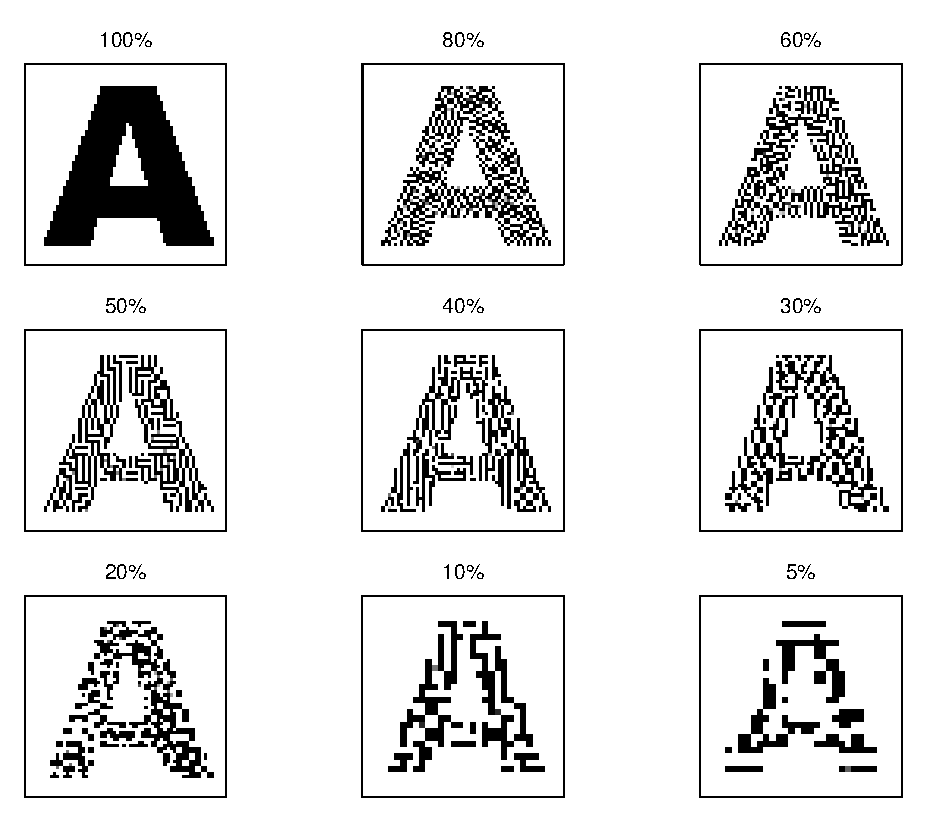
\includegraphics [scale = 0.6]{images/compression-walsh-2d.eps}
% \includegraphics [scale = 0.6]{images/compression-walsh-2d-2.eps}
    \end{center}
    \caption{Compress a 2D image}
              \label{fig-compression-walsh-2d}
\end{figure}
\end{enumerate}
\end{exo}
 
 
\begin{exo}[Hadamard matrices]
\label{exo-matrices-hadamard}
\index{Matrix!of Hadamard} \index{Hadamard@\nompropreindex{Hadamard}} \index{Determinant!maximal} This exercise makes the connection between the Walsh matrices considered in paragraph~\ref{sect2-presentation-transforme-walsh} and the quadratic residuals introduced at the beginning of this chapter. A matrix $ H_n $, of size $ n \times n $, whose inputs are $ + 1 $ or $ -1 $, is called a Hadamard matrix if it satisfies
\begin{equation*}
H_n \transp{H_n} = n \Id_n,
\end{equation*}
where we denote by $ \transp{H_n} $ the transposed matrix of $ H_n $. \begin{enumerate}
\item Explain why the matrix $ W_n $, defined in the proposition \ref{prop-pte-matrix-hadamard}, for $ n = 2^k $, is a Hadamard matrix.
\item Show that if there exists a Hadamard matrix $ H_n $ of size $ n \times n $, then $ n $ is worth $ 1 $, or $ 2 $, or is a multiple of $ 4 $. We can start by showing that we can assume that $ H_n $ is normalized, that is to say with $ 1 $ on the first row and the first column. Then we will show that if $ n \geq 3 $, we can assume that the first three lines of $ H_n $ are written in the form
\begin{equation*}
\begin{array}{cccc} \underbrace{\begin{matrix} 1 & \ldots & 1 \\1 & \ldots & 1 \\1 & \ldots & 1 \end{matrix}} & \underbrace{\begin{matrix} 1 & \ldots & 1 \\1 & \ldots & 1 \\-1 & \ldots & -1 \end{matrix}} & \underbrace{\begin{matrix} 1 & \ldots & 1 \\-1 & \ldots & -1 \\1 & \ldots & 1 \end{matrix}} & \underbrace{\begin{matrix} 1 & \ldots & 1 \\-1 & \ldots & -1 \\- 1 & \ldots & -1 \end{matrix}} \\i & j & k & l \end{array}
\end{equation*}
where the integers $ i $, $ j $, $ k $, and $ l $ denote the lengths of each portion (they can optionally be zero). Finally, we will show that we actually have $ i = j = k = l $.
\item \index{Paley@\nompropreindex{Paley}} \index{Matrix!of Paley} \index{Quadratic residue} The inverse problem, namely the construction of a matrix $ H_n $ for a $ n $ multiple of $ 4 $ given, is very complex. In fact, it is speculated that it is still possible to do so, although it has not yet been proven. Assume that $ n = p + 1 $, where $ p $ is an odd prime number. We also suppose that $ n $ is a multiple of $ 4 $, and we will show that we can then construct a matrix $ H_n $. We will use the quadratic residue character modulo $ p $, denoted by $ \eta $, which is defined in the equation \eqref{eq-defn-cartactere-eta}. We define a matrix $ Q $ of size $ p \times p $ by
\begin{equation*}
Q \eqdef \left\{\eta (ji) \right\}_{0 \leq i, \, j \leq p-1}.
\end{equation*}
Show that $ Q $ is anti-symmetric, and that we have $ Q \transp{Q} = p \Id_p - J $, where $ J $ is the matrix whose all inputs are worth $ 1 $. Also show that we have $ QJ = JQ = 0 $. Such a matrix is called \textit{Paley matrix}.
\item We now define the matrix $ H_n $ of size $ n \times n $ by
\begin{equation*}
H_n \eqdef \begin{pmatrix} 1 & v \\\transp{v} & Q- \Id_p \end{pmatrix},
\end{equation*}
where we noted $ v = (1, \ldots, \, 1) \in \RR^p $. Show that $ H_n $ is a Hadamard matrix. Here is an example for $ p = $ 7:
\begin{equation*}
H_8 \eqdef \begin{pmatrix} 1 & 1 & 1 & 1 & 1 & 1 & 1 & 1 \\1 & -1 & 1 & 1 & -1 & 1 & -1 & -1 \\1 & -1 & -1 & 1 & 1 & -1 & 1 & -1 \\1 & -1 & -1 & -1 & 1 & 1 & -1 & 1 \\1 & 1 & -1 & -1 & -1 & 1 & 1 & -1 \\1 & -1 & 1 & -1 & -1 & -1 & 1 & 1 \\1 & 1 & -1 & 1 & -1 & -1 & -1 & 1 \\1 & 1 & 1 & -1 & 1 & -1 & -1 & -1 \end{pmatrix}.
\end{equation*}
 
\item Let $ A $ be a matrix of size $ n \times n $ such that its inputs $ a_{ij} $ verify
\begin{equation*}
\forall (i, \, j) \in \{1, \ldots, \, n\}^2, \quad | a_{ij} | \leq 1.
\end{equation*}
Show the Hadamard inequality:
\begin{equation}
\label{eq-borne-hadamard}
| \det (A) | \leq n^{\frac{n}{2}}.
\end{equation}
Show that if there is a Hadamard matrix, then the latter reaches this bound.
\end{enumerate} The geometric interpretation of the bound \eqref{eq-borne-hadamard} is very simple. It is a matter of considering a system of $ n $ vectors (the columns of the matrix) inside the cube $ | x_i | \leq 1 $, (where we denote by $ \{x_i\}_{i = 1}^n $ a coordinate system), enclosing a rectangular parallelepiped of maximum volume. In the case of Hadamard matrices, these vectors are large diagonals of the cube, and therefore have maximum lengths. In addition, they are orthogonal, so as to produce the maximum volume. In dimensions where Hadamard matrices do not exist, it is not possible to produce orthogonal diagonals, even if one thinks that the vectors which minimize \eqref{eq-borne-hadamard} are close to the large diagonals . This remains an open problem. \\The exercise \oldref{exo-codes-hadamard} presents an application of Hadamard matrices for the construction of bi-orthogonal corrective codes.
\end{exo}
 
 
\begin{exo}[Matrix tensor product]
\label{exo-tensor-product}
\index{Tensor product} Let $ A $ be a square matrix of size $ s $ and $ B $ a square matrix of size $ t $. We define the tensor product $ A \otimes B $ as the matrix of size $ s \times t $
\begin{equation*}
A \otimes B \eqdef \begin{pmatrix} a_{11} B & \cdots & a_{1s} B \\\vdots & & \vdots \\a_{s1} B & \cdots & a_{ss} B \end{pmatrix}.
\end{equation*}
\begin{enumerate}
\item We assume that $ A $ matches $ AA^* = s \Id_s $. Show that $ A^{\otimes n} = A \otimes \cdots \otimes A $ ($ n $ products) satisfies $ A^{\otimes n} (A^{\otimes n})^* = s^n \Id_{s^n} $.
\item What is the connection with the Walsh transform?
\item Taking inspiration from the fast FWT algorithm, write a fast algorithm that computes the transform $ y = A^{\otimes n} x $. How is the inverse transform calculated?
\item We take as base matrix
\begin{equation*}
A_\alpha \eqdef \sqrt{2} \begin{pmatrix} \cos (\alpha) & \sin (\alpha) \\\sin (\alpha) & - \cos (\alpha) \end{pmatrix}.
\end{equation*}
How can the transform $ x \mapsto A_\alpha^{\otimes n} x $ be seen as an intermediate Walsh transform?
\end{enumerate} The figure \figref{fig-transfo-walsh-interm} shows the transforms of a \guill{triangle} function for values of $ \alpha $ in $ [0, \pi / 2] $. The ordinary Walsh transform corresponds to the \ordin{6}{th} curve. For $ \alpha = \pi / 2 $, we find the original symmetrized signal. \begin{figure}[ht]
    \begin{center}
    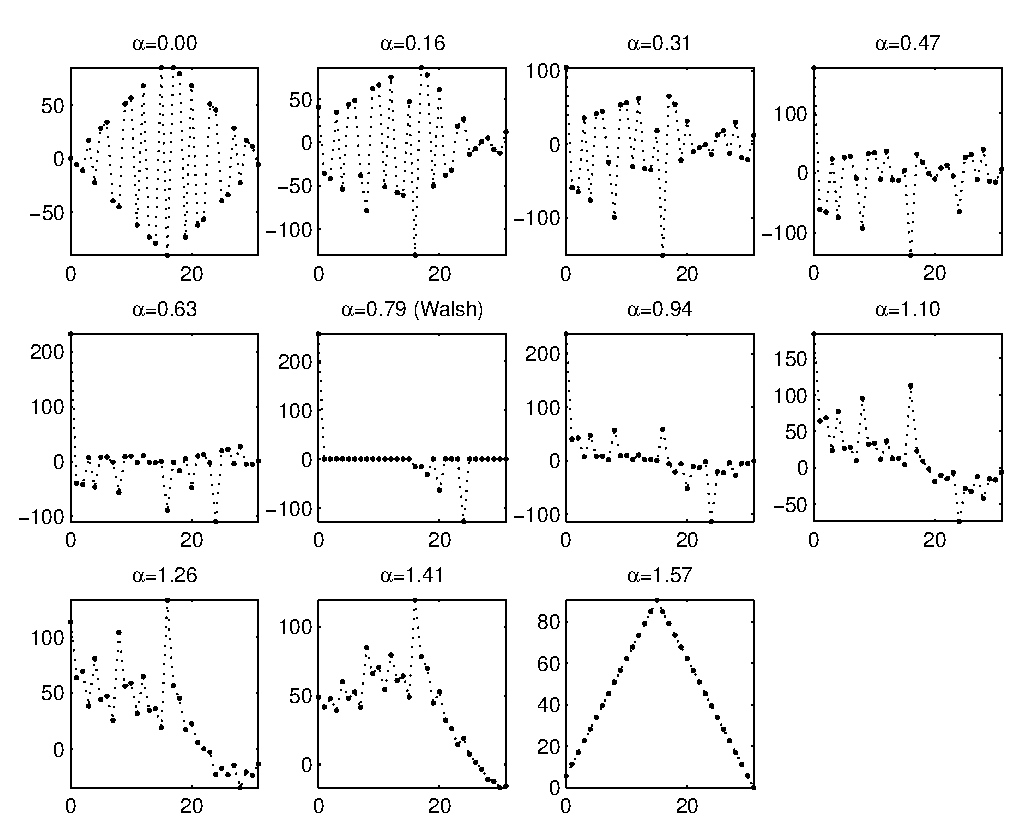
\includegraphics [scale = 0.7]{images/transfo-walsh-interm.eps}
% \includegraphics [scale = 0.7]{images/transfo-walsh-interm-2.eps} BUG?
    \end{center}
    \caption{Intermediate Walsh transform}
              \label{fig-transfo-walsh-interm}
\end{figure}
We can look at the exercise \oldref{exo-grpe-quaternionique}, which uses the theory of linear representations to build a matrix $ A $ of size $ 8 $.
\end{exo}
 
 
\begin{exo}[Generalization of the identity of MacWilliams]
\label{exo-generalization-mac-williams}
 
\index{MacWilliams@\nompropreindex{MacWilliams}} \index{Identity!of MacWilliams} In this exercise, we propose to extend the identity of MacWilliams to the case of the vector space $ E = \FF_q^k $. \begin{enumerate}
\item We define the following bilinear form on $ E \times E $, with value in $ \FF_q $:
\begin{equation*}
\forall (a, \, x) \in E^2, \quad \dotp{a}{x} \eqdef \sum_{i = 0}^{p-1}{a_i x_i}.
\end{equation*}
Explain how it represents the bilinear form of the duality (bracket of the duality) between the space $ E $ and its dual $ E^* $ (correctly identified as $ E $).
\item We denote by $ \chi_1 $ the canonical additive character of $ \FF_q $, as defined by the equation \eqref{defn-character-additive-canonical}. Let $ a = \{a_0, \ldots, \, a_{k-1}\} \in (\ZZ/q \ZZ)^k $. We define
\begin{equation*}
\chi_a: \func{E}{\CC^*}{x}{\chi_1 (\dotp{a}{x})}.
\end{equation*}
Explain why the applications $ \chi_a $ allow to define an isomorphism between $ E $ and its dual as an additive group, $ \wh{E} $.
\item \index{Subgroup} \index{Orthogonal!of a vector space} \index{Orthogonal!of a subgroup} Let $ H $ be a subgroup of $ E $. Show that it is also a vector subspace. Deduce from the previous question that we can identify the orthogonal of $ H $ for the group structure, noted $ H^{\sharp} $, and that for the vector space structure, noted $ H^{\bot} $.
\item Demonstrate the identity of MacWilliams within the $ E $ space:
\begin{equation*}
A_{H^{\bot}} (X, \, Y) = \frac{1}{| H |} A_{H} (X + (q-1) Y, \, XY).
\end{equation*}
\end{enumerate}
\end{exo}
 
 
\begin{exo}[Poisson formula and distributions]
\label{exo-formula-fish-distrib}
\index{Distribution} \index{Dirac comb} \label{notation-41} This exercise requires some knowledge of distribution theory, in particular the definition of the Fourier transform of a distribution. Here we take as convention the transform defined in the equation \eqref{eq-transforme-fourier-R}, which differs by a factor of $ 2 \pi $ from that used in \eqref{eq-defn-trans-fourier-special-fish}. We denote by $ \Pi_s $ the Dirac comb of steps $ s $, that is to say
\begin{equation}
\label{eq-trans-fourier-comb-dirac}
\Pi_s \eqdef \sum_{k \in \ZZ}{\delta_{ks}},
\end{equation}
\index{Support!compact} where $ \delta_t $ is the distribution defined by $ \dotp{\delta_t}{\varphi} \eqdef \varphi (t) $ for $ \varphi \in \Cc^\infty_0 (\RR ) $ (functions of class $ \Cc^\infty $ with compact support). Show that the Poisson formula \eqref{eq-formula-fish-continue} implies the following equality:
\begin{equation*}
\wh{\Pi_s} = \frac{2 \pi}{s} \Pi_{\frac{2 \pi}{s}}.
\end{equation*}
\end{exo}
 
 
\begin{exo}[Shannon sampling]
\label{exo-sample-shannon}
 
\index{Shannon@\nompropreindex{Shannon}} \index{Sampling!theorem} \index{Sampling} Let $ T> 0 $. We notice
\begin{equation*}
I_T \eqdef \left[- \frac{\pi}{T}, \, \frac{\pi}{T} \right] \quad \text{et} \quad E_T \eqdef \enscond{f \in L^2 (\RR)}{\Supp (\wh{f}) \subset I_T}.
\end{equation*}
Let $ f \in E_T $. We want to prove Shannon's sampling theorem, which says that $ f $ can be reconstructed (interpolated) from the samples $ f(n T) $, for $ n \in \ZZ $. More precisely, if we note
\begin{equation}
\label{eqn-formula-reconstruction-shannon}
\sinc_T (t) \eqdef \frac{\sin \left(\ofrac{\pi t}{T} \right)}{\ofrac{\pi t}{T}},
\end{equation}
so we want to show that
\begin{equation*}
f(t) \eqdef \sum_{n \in \ZZ}{f(n T) \sinc_T (tn T)}.
\end{equation*}
\begin{enumerate}
\item Show that $ f $ is of class $ \Cc^\infty $.
\item We denote by $ f_d $ the distribution which corresponds to the sampling of $ f $:
\begin{equation*}
f_d \eqdef \sum_{n \in \ZZ}{f(n T) \delta_{n T}}.
\end{equation*}
Using the equality \eqref{eq-trans-fourier-comb-dirac}, show that we have
\begin{equation*}
| \omega | \leq \frac{\pi}{T} \Longrightarrow \wh{f_d} (\omega) = \frac{1}{T} \wh{f} (\omega).
\end{equation*}
 
\item Calculate the inverse Fourier transform of the indicator function of the interval $ I_T $. Deduce the sampling theorem.
\item \index{Hilbert basis} \index{Orthogonal!projection} Show that the family $ \{t \mapsto \sinc_T (t n T)\}_{n \in \ZZ} $ forms an orthogonal base (base de Hilbert) of the space $ E_T $. How is the projection of a function $ f \in L^2 (\RR) $ calculated on this space?
\end{enumerate}
\end{exo}

\chapter{Discrete Fourier transform}
\label{chap-tfd} 
 
 
The use of the discrete Fourier transform is at the base of almost all digital digital algorithms. The discovery of the fast transformation algorithm \textit{FFT} (for \textit{\textbf{F}ast \textbf{F}ourier \textbf{T}ransform}, in French \textit{Transformée de Fourier Rapide}) revolutionized the world of signal processing by allowing digital calculations in reasonable time. It was largely this discovery that made it clear that we could work as quickly in the digital world (made up of discrete signals) as in the analog world (made up of continuous signals). Further details on the history of this discovery, and its consequences, can be found in the article by \nompropre{Rockmore} \cite{rockmore-fft}. More than a simple particular case of the Fourier transform on a finite group, the discrete Fourier transform has its own language and especially efficient algorithms that are much less obvious than the clear formulas of the previous chapter. This chapter aims in a way to take a tour of the owner; it shows in any case that the multitude of existing FFT algorithms is impressive. But the most important thing, beyond a total understanding of the different variations of the algorithm, is to perceive the strategy of the algorithm, in order to be able to decide, if necessary, which implementation to use.
 
The FFT algorithm in temporal decimation version is relatively well described (and especially well implemented) in the \nompropre{Numerical Recipes} \cite{nr}. Regarding the frequency decimation version as well as many improvements, we refer to the book by \nompropre{Brigham} \cite{brigham-fft}. For implementation details in C language, we can look at the book by \nompropre{Arnt} \cite{arndt-algo-programmers}.
 
% ------------------------------------------------- -----
% ------------------------------------------------- -----
% ------------------------------------------------- -----
% section - The language of signal processing                            
% ------------------------------------------------- -----
% ------------------------------------------------- -----
% ------------------------------------------------- -----
\section{The language of signal processing}
% \addcontentsline{toc}{section}{The signal processing language}
\label{sect1-language-processing-signal} 
 
 
In this paragraph, we will translate the algebraic properties of the Fourier transform into the language of discrete signal theory. First, we will restrict ourselves to a one-dimensional study (to present the algorithms and some applications), then we will make the link between the Fourier transform on an abelian product group and the discrete Fourier transform in dimension two and more.
 
 
\index{Signal} \label{notation-42} To fix the ideas, we will consider time signals with complex values. These correspond to functions $ \wt{f}: t \in \RR \rightarrow \wt{f} (t) \in \CC $. To process this signal digitally, we will only consider a finite number of signal values, and work on these values. We will therefore name the sample of size $N$ of the original signal $ \wt{f} $ the vector $ f \eqdef \{f[n]\}_{n = 0}^{N-1} $, where the we have denoted $ f[n] \eqdef \wt{f} (t_n) $ the value of the signal $ f $ at the instant $ t_n $. The notation in braces is meant to remind that we consider our vectors as samples of a (continuous) signal, but it will happen that we consider these elements as simple vectors of $ \CC^N $. So that the following analysis is not biased (particularly when reconciling with the continuous transform in Section~\ref{sect1-link-trans-fourier-R}), the values of $ \left\{t_n \right\}_{n = 0}^{N-1} $ are assumed to be evenly spaced in an interval $ [a, b] $, i.e. $ t_n = a + \frac{ba}{N} n $.
 
\begin{defn}[Discrete Fourier transform]
\index{Discrete Fourier transform} \label{notation-43} We define the \textit{Discrete Fourier transform} (abbreviated \textit{TFD}) of the sample $ f = \{f[n]\}_{n = 0}^{N-1} $ as being the vector $ \wh{f} = \{\wh{f}[k]\}_{k = 0}^{N-1} \in \CC^N $ with
\begin{equation}
\label{eq-defn-tfd}
\wh{f}[k] \eqdef \sum_{n = 0}^{N-1}{f[n] \omega_N^{- nk}} \quad \quad \quad \text{for} k = 0 , \ldots, \, N-1,
\end{equation}
where we denote $ \omega_N = e^{\frac{2 \imath \pi}{N}} $ a primitive \ordin{N}{ième} root of the unit. \\We will also denote $ \Ff(f) \eqdef \wh{f} $, which allows to define
\begin{equation*}
\Ff: \func{\CC^N}{\CC^N}{f}{\Ff(f) = \wh{f}}.
\end{equation*}
This notation can lead to confusion with the Fourier transform on a finite group defined by the equation \eqref{eq-transf-fourier-grpe-abelien}, however, the great similarity between the two applications (all this is justified a bit below) makes it convenient to use the same notation.
\end{defn}
 
 
\begin{rem}
We could have chosen another primitive root of the unit instead of $ \omega_N $. This amounts to choosing another generator for the starting group $ \ZZ/N \ZZ $, and therefore to numbering the elements of $ f $ in a different order.
\end{rem}
 
 
\begin{rem}{(\upshape \textbf{Link with the Fourier transform on a finite group}).} 
\index{Fourier transform!on a finite group} We have already seen in Section~\ref{sect1-dual-cyclic-group}, that the characters $ (\chi_k)_{k = 0}^{N-1 } $ on the cyclic group $ \ZZ/N \ZZ $ can be defined by
\begin{equation}
\label{eq-formula-character-znz}
\forall s \in \ZZ/N \ZZ, \quad \chi_k (s) \eqdef \omega_N^{- ks}.
\end{equation}
We notice that our sample $ f \in \CC^N $ allows to define a function $ f_1: \ZZ/N \ZZ \rightarrow \CC $, and vice versa. We can make the link between discrete Fourier transform and characters:
\begin{equation*}
\wh{f}[k] = \wh{f_1} (\chi_k).
\end{equation*}
We can therefore rewrite the Fourier inversion formula of the proposition \ref{prop-decomposition-serie-fourier}, in terms of a discrete Fourier transform.
\end{rem}
 
 
\begin{prop}[Inverse Fourier transform]
\label{prop-tfd-inverse}
\index{Fourier transform!inverse} We have the following inversion formula:
\begin{equation}
\label{eq-transforme-fourier-discr-inverse}
\forall n = 0, \ldots, \, N-1, \quad f[n] = \frac{1}{N} \sum_{k = 0}^{N-1}{\wh{f}[ k] \omega_N^{nk}}.
\end{equation}
\end{prop}
 
 
\begin{cor}
$ \Ff: \CC^N \rightarrow \CC^N $ is an isomorphism of vector spaces.
\end{cor}
Let us also recall Plancherel's formula.
 
\begin{prop}[Plancherel formula]
\label{prop-formula-floorel-tfd}
\index{Plancherel's formula} Let $ f $ and $ g $ be two samples of size $N$. We have the following formula:
\begin{equation*}
\sum_{i = 0}^N{f[i] \ol{g [i]}} = \frac{1}{N} \sum_{i = 0}^N{\wh{f}[i] \ol{\wh{g}[i]}}.
\end{equation*}
\end{prop}
 
% ------------------------------------------------- -----
% ------------------------------------------------- -----
% ------------------------------------------------- -----
% section - Fast Fourier transform                            
% ------------------------------------------------- -----
% ------------------------------------------------- -----
% ------------------------------------------------- -----
\section{Fast Fourier transform}
% \addcontentsline{toc}{section}{Fast Fourier transform}
\label{sect1-transform-fast} 
 
 
This paragraph is aimed directly at the IT applications of the TFD. It does not require knowledge of group theory. The connections between the FFT algorithm and algebra are discussed in some exercises, for example when studying the \textit{Good-Thomas} \oldref{exo-algo-good-thomas} method. In parallel with the reading of this chapter, it is of course necessary to have a{\oe} on the algorithms referenced in Paragraph~\ref{sect1-listing-fft}, to make the link between concrete implementation and mathematical formulas.
% ------------------------------------------------- -----
% ------------------------------------------------- -----
% sub-section - Presentation of the algorithm                            
% ------------------------------------------------- -----
% ------------------------------------------------- -----
\subsection{Presentation of the algorithm}
\label{sect2-present-algo-fft} 
 
 
\index{Fast Fourier transform} \index{FFT} \index{Algorithm!FFT} For a signal $ f $ of which we know a sample $ \{f[n]\}_{n = 0}^{N -1} $, the direct calculation of the $N$ coefficients of the discrete Fourier transform
\begin{equation}
\label{eq-calcul-direct-tfd}
\wh{f}[k] \eqdef \sum_{n = 0}^{N-1}{f[n] e^{- kn \frac{2 \imath \pi}{N}}} \quad \quad \quad \text{for} k = 0, \ldots, \, N-1
\end{equation}
requires $ 2 N^2 $ operations (complex addition and multiplication). The \textit{FFT} algorithm allows, by reordering the computations in a dichotomous way, to considerably reduce the computation time by bringing it back to an order of $ O(N \log (N)) $. Throughout this chapter, we are going to present different versions of the FFT algorithm, starting with the original version, and arguably the simplest, the \nompropre{Cooley} and \nompropre{Tukey} algorithm. However, we will see that this algorithm has been declined in an almost infinite number of more learned versions than the others, to adapt to different conditions (length of vectors mainly), and to obtain the result always more quickly. Behind a seemingly very simple transformation, TFD, therefore hides a multitude of ideas of a combinatorial and algebraic nature.
 
 
Before embarking on a perilous description of the algorithm, let us note a reassuring fact: we will be able to easily reinvest our algorithm to calculate the inverse transform, as specified in the following remark.
 
\begin{rem}{(\upshape \textbf{Inverse transform}).} 
\index{Fourier transform!inverse} We notice that the inverse transform formula \eqref{eq-transforme-fourier-discr-inverse} can be obtained by replacing $ \omega_N $ by $ \omega_N^{-1} $ in the calculation algorithm, then dividing the result by $N$. Consequently, we can also calculate the inverse discrete Fourier transform in time $ O(N \log (N)) $, obviously modifying the algorithm used. More synthetically, by considering the sample $ \{f_1 [n]\}_{n = 0}^{N-1} $ defined by
\begin{equation*}
\forall n \in \{1, \ldots, \, N-1\}, \quad f_1 [n] = \frac{1}{N} f[Nn] \quad \quad f_1 [0] \eqdef \frac{1}{N} f[0],
\end{equation*}
we have a writing of the inverse Fourier transform of $ f $ in terms of a direct Fourier transform:
\begin{equation*}
\Ff^{-1} (f) = \Ff(f_1)
\end{equation*}
\end{rem}
 
 
 
\index{Dichotomy} \index{Divide and conquer} \index{Cooley-Tukey@\nompropreindex{Cooley-Tukey}} The algorithm we are about to describe was discovered by \nompropre{Cooley} and \nompropre{Tukey } in 1965. It allows, when we have a \guill{good} decomposition of the integer $N$, to calculate the discrete Fourier transform very quickly. We will see in the remainder of the presentation of other algorithms which make it possible to exploit certain less optimal decompositions of $N$. However, in this first approach of the FFT algorithm, we will assume that $ N = 2^p $. This very simple factorization of $N$ will make it possible to use the famous \guill{philosophy} \textit{divide and reign}, by performing a dichotomous progression in the calculation of the TFD. To implement this dichotomy, let us group the terms of the sum of a DFT according to the parity of the indices. \\We obtain then, for $ k \in \{0, \ldots, \, N-1\} $,
\begin{align}
\wh{f}[k] = & \sum_{n = 0}^{N / 2-1}{f[2 n] e^{- 2 \imath \pi k (2 n) / N}} + \sum_{n = 0}^{N / 2-1}{f[2 n + 1] e^{- 2 \imath \pi k (2n + 1) / N}} \\
\label{eq-fft-dif}
= & \sum_{n = 0}^{N / 2-1}{f[2 n] e^{- 2 \imath \pi kn / (N / 2)}} + \omega_N^{- k} \sum_{n = 0}^{N / 2-1}{f[2 n + 1] e^{- 2 \imath \pi kn / (N / 2)}},
\end{align}
where we noted $ \omega_N = e^{2 \imath \pi / N} $. So if we write \label{notation-44}
\begin{align}
\label{eq-part-even-odd}
f^0 & \eqdef \left\{f[0], \, f[2], \ldots, \, f[N-2] \right\} \\
f^1 & \eqdef \left\{f[1], \, f[3], \ldots, \, f[N-1] \right\}
\end{align}
the vectors of even (resp. odd) indices formed from $ f $, we notice that for the $ N / 2 $ first indices $ k \in \{0, \, 1, \ldots, \, N / 2-1\} $, the equation \eqref{eq-fft-dif} is written as the sum of two discrete Fourier transforms:
\begin{equation}
\label{eq-danielson-lanczos-1}
\wh{f}[k] = \wh{f^0}[k] + \omega_N^{- k} \wh{f^1}[k].
\end{equation}
For the indices $ k \in \{N / 2, \ldots, \, N-1\} $, if we write $ k'= kN / 2 $, using the fact that the vectors $ \wh{f^0} $ and $ \wh{f^1} $ represent samples of period $ N / 2 $, and that $ \omega_N^k = - \omega_N^{k'} $ this time we get the difference of two transforms from Fourier:
\begin{equation}
\label{eq-danielson-lanczos-2}
\wh{f}[k] = \wh{f^0}[k'] - \omega_N^{- k'} \wh{f^1}[k'].
\end{equation}
 
 
\begin{defn}[Some notations]
\index{Operator!$ \Ss $} \label{notation-45} \label{notation-46} To summarize all this in a more algorithmic form, let us note
\begin{align}
\label{eq-part-gd}
\wh{f}_g & \eqdef \left\{\wh{f}[0], \, \wh{f}[1], \ldots, \, \wh{f}[N / 2-1] \right\} \\
\wh{f}_d & \eqdef \left\{\wh{f}[N / 2], \, \wh{f}[N / 2 + 1], \ldots, \, \wh{f}[N -1] \right\}.
\end{align}
These are the right and left parts of the transformed vector $ \wh{f} = \Ff(f) $. We will also define the operator $ \Ss_N^x $, for $ x \in \RR $, which takes a vector $ a = \{a_0, \ldots, \, a_{N-1}\} \in \CC^N $ of length $N$ and returns
\begin{equation}
\label{eq-operator-S}
\Ss_N^xa \eqdef \left\{a_j e^{- xj \frac{2 \imath \pi}{N}} \right\}_{j = 0}^{N-1} = \left\{a_j \omega_N^{- xj} \right\}_{j = 0}^{N-1} \in \CC^N.
\end{equation}
\end{defn}
We then have the very simple expression of the recurrence that we will use to implement the FFT algorithm: \index{Equation!Danielson-Lanczos}
\begin{align}
\label{eq-danielson-lanczos-a}
\wh{f}_g & = \wh{f^0} + \Ss_{N / 2}^{1/2} \wh{f^1} \\
\label{eq-danielson-lanczos-b}
\wh{f}_d & = \wh{f^0} - \Ss_{N / 2}^{1/2} \wh{f^1}.
\end{align}
\index{Decimation!temporal} The equations \eqref{eq-danielson-lanczos-a} and \eqref{eq-danielson-lanczos-b}, also called equations of \textit{Danielson-Lanczos}, express the fact that the Discrete Fourier transform of a signal of length $N$ can be calculated as a function of two signals of length $ N / 2 $, here noted $ f^0 $ and $ f^1 $. We call this approach \textit{decimation in time} (in English \textit{Decimation In Time}, or \textit{DIT}), as opposed to another approach, the \textit{frequency decimation}, which will be described quickly in paragraph \ref{sect2-frequency-decimation}. It is the temporal decimation that will be developed (and optimized) in the next paragraph, but first of all, let's start by presenting a naïve implementation.
 
\begin{rem}{(\upshape \textbf{The butterfly effect}).} 
\index{Iteration} \index{Diagram!butterfly} The operation consisting in mixing two inputs of the even and odd parts of a vector by following the equations \eqref{eq-danielson-lanczos-a} and \eqref{eq-danielson-lanczos-b} is called \textit{butterfly scheme} (in English \textit{butterfly scheme}). The figure \figref{fig-fft-butterfly-2points} schematically shows the operations performed. It also gives an idea of the cabling to be carried out to perform such an operation directly on a card dedicated to signal processing. Indeed, as shown in figure \figref{fig-fft-butterfly-8points}, an iteration in the FFT algorithm (here for an input of size $ 8 $) is only a succession of butterfly diagrams carried out in cascade . \begin{figure}[ht]
    \begin{center}
    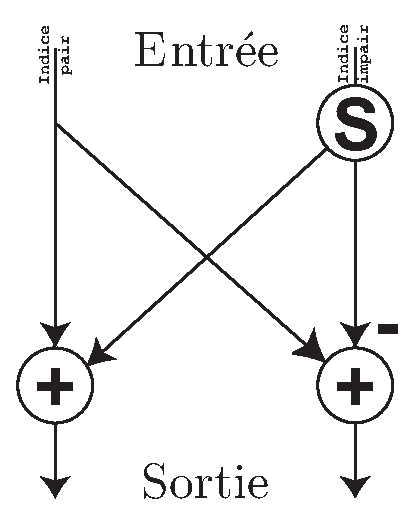
\includegraphics [scale = 0.7]{images/fft-butterfly-2points.eps}
    \end{center}
    \caption{Elementary butterfly diagram}
              \label{fig-fft-butterfly-2points}
\end{figure}
\begin{figure}[ht] 
    \begin{center}
    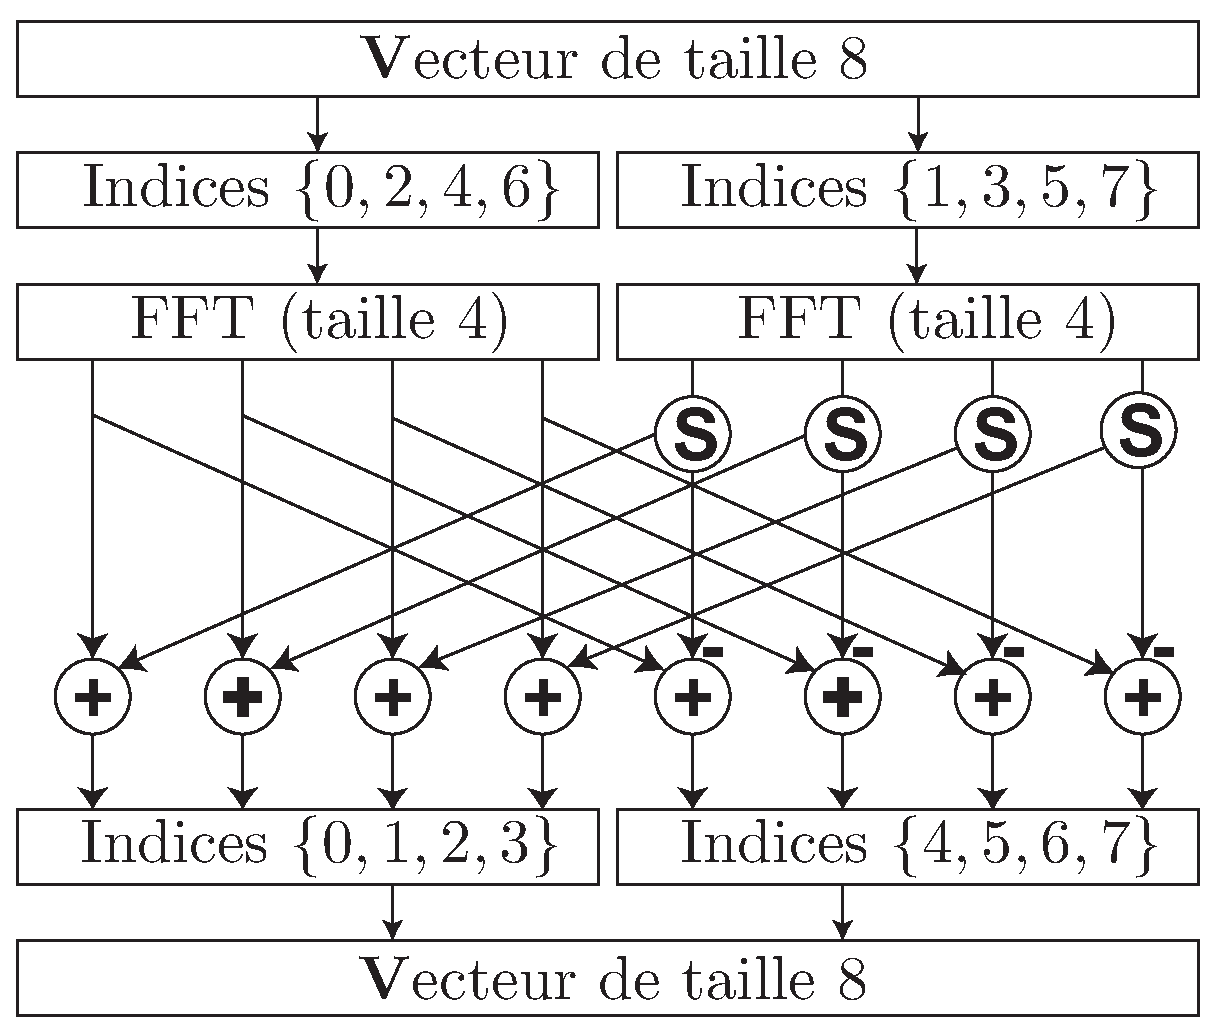
\includegraphics [scale = 0.5]{images/fft-butterfly-8points.eps}
    \end{center}
    \caption{An iteration of the FFT algorithm}
              \label{fig-fft-butterfly-8points}
\end{figure}
\end{rem}
 
 
 
\index{Algorithm!recursive} The simplest way to implement{\oe} the equations \eqref{eq-danielson-lanczos-a} and \eqref{eq-danielson-lanczos-b} is to use a recursive procedure. It is a known fact that a recursive procedure can be written, by means of loops, in a non-recursive fashion (but this process can sometimes be dangerous). We will see in the next paragraph \ref{sect2-impl-concrete} that the FFT algorithm has a lot to gain from being written non-recursively, and not only because of saving time. But for educational purposes, and in order to present some optimizations that can be done on the FFT implementation, we will focus on the recursive implementation written in the \ref{sect1-listing-fft} section.
 
 
The procedure \texttt{fft \_rec} therefore takes as input an integer \texttt{dir} which is worth $ + 1 $ or $ -1 $ depending on whether the Fourier transform is direct or inverse. To simplify the understanding of the code, a procedure \texttt{operator \_s} has been written to realize the operator $ \Ss^x_N $: it takes as input a vector as well as a real number $ x $ (which depends on the sign of the transform).
% ------------------------------------------------- -----
% ------------------------------------------------- -----
% sub-section - Cost analysis                            
% ------------------------------------------------- -----
% ------------------------------------------------- -----
\subsection{Cost analysis}
\label{sect2-analyze-cost-fft} 
 
Using the recurrence equations \eqref{eq-danielson-lanczos-a} and \eqref{eq-danielson-lanczos-b}, we easily calculate the cost of the algorithm.
 
\begin{prop}[Complexity of the FFT]
\index{Complexity} If we denote by $ C (N) $ the cost of the FFT algorithm for an input of length $N$, then $ C (N) $ satisfies the functional equation
\begin{equation*}
C (N) = 2 C (N / 2) + KN,
\end{equation*}
where $ K $ is some constant. In the end, we arrive at the expression $ C (N) = KN \log_2 (N) $.
\end{prop}
\begin{proof}
Computing $ \wh{f} $ requires computing $ \wh{f^1} $ and $ \wh{f^2} $ (i.e. $ 2 C (N / 2) $ operations), then mixing the two transforms by the butterfly diagram (i.e. $ KN $ operations). To reduce to a linear recurrence, it suffices to set $ P = \log_2 (N) $, and $ C'(N) = \frac{C (N)}{N} $ satisfies the functional equation $ C' (P) = C'(P-1) + K $. As $ C'(0) = 0 $, we deduce $ C' (P) = KP $, which allows us to conclude.
\end{proof}
The FFT algorithm may seem a bit magical, the fact remains that its discovery made it possible to make many calculations possible by reducing the cost of calculating $N$ Fourier coefficients by $ O(N^2) $ for a naive approach to $ O(N \log (N)) $. Its fairly recent discovery (in the mid-1960s) was a mini revolution: a calculation which until then required two weeks on a computer of the time was suddenly achievable in barely thirty seconds \footnote{Source: \cite{nr}, for $N$ of the order of $ 10^6 $}.
% ------------------------------------------------- -----
% ------------------------------------------------- -----
% sub-section - Variations around the algorithm                            
% ------------------------------------------------- -----
% ------------------------------------------------- -----
\subsection{Variations around the algorithm}
\label{sect2-variations-fft} 
 
Before describing a more efficient implementation of the FFT algorithm, let's make some additional remarks, which provide many variations around the proposed recursive implementation.
 
\begin{rem}{(\upshape \textbf{Length of entries}).} 
In the case where the length $N$ of the data of a sample $ \{f[n]\}_{n = 0}^{N-1} $ is not a power of two, we can make a calculation approximated by completing the sample with a sequence of zeros, to obtain a sample $ \{f_1 [n]\}_{n = 0}^{M-1} $, with $ M = 2^p $. Of course, we no longer calculate exactly the same transform, but in the case of an approximate calculation (calculation of continuous transforms, as explained in Section~\ref{sect1-link-trans-fourier-R}), this amounts to calculating the transform at slightly different frequencies, which is often acceptable.
\end{rem}
 
 
\begin{rem}{(\upshape \textbf{Calculation basis}).} 
\label{rmk-radix-fft}
\index{FFT!in base 4} The equations \eqref{eq-danielson-lanczos-a} and \eqref{eq-danielson-lanczos-b} which we used to implement the algorithm are the consequence of the sharing of vectors into two sub-vectors of size $ N / 2 $. This is called an FFT in \textit{base 2} (\textit{radix-2} in English). We can think of using another base, for example 4, which leads to considering sums of the four sub-FFTs of length $ N / 4 $. The advantage of such a choice (compared to base 2) is that one avoids making the obvious calculations of the fourth roots of the unit (which are coded simply by subtractions instead of additions in the formulas), which slightly reduces the number of operations to be performed. On the other hand, we must be careful, because the signs are not the same for the direct transform and for the reverse transform. To write the notations, we introduce the sub-vectors $ f^0 $, $ f^1 $, $ f^2 $ and $ f_3 $, of length $ N / 4 $, which are constructed from $ f $ in considering only the indices congruent respectively to 0, 1, 2 and 3 modulo 4. We also use $ \sigma $ which is worth $ + 1 $ for the direct transform, and $ -1 $ for the inverse transform. To discern the different portions of length $ N / 4 $ of the result, we will write $ \wh{f}^{(0/4)} $ for the first quarter, etc. Here are the equations:
\begin{align*}
\wh{f}^{(0/4)} & = \Ss_{N / 4}^{0/4} \wh{f^0} & + & \quad \Ss_{N / 4}^{1 / 4} \wh{f^1} & + & \quad \Ss_{N / 4}^{2/4} \wh{f^2} & + & \quad \Ss_{N / 4}^{3 / 4} \wh{f^3} \\
\wh{f}^{(1/4)} & = \Ss_{N / 4}^{0/4} \wh{f^0} & - & \quad \imath \sigma \Ss_{N / 4 }^{1/4} \wh{f^1} & - & \quad \Ss_{N / 4}^{2/4} \wh{f^2} & + & \quad \imath \sigma \Ss_{N / 4}^{3/4} \wh{f^3} \\
\wh{f}^{(2/4)} & = \Ss_{N / 4}^{0/4} \wh{f^0} & - & \quad \Ss_{N / 4}^{1 / 4} \wh{f^1} & + & \quad \Ss_{N / 4}^{2/4} \wh{f^2} & - & \quad \Ss_{N / 4}^{3 / 4} \wh{f^3} \\
\wh{f}^{(3/4)} & = \Ss_{N / 4}^{0/4} \wh{f^0} & + & \quad \imath \sigma \Ss_{N / 4 }^{1/4} \wh{f^1} & - & \quad \Ss_{N / 4}^{2/4} \wh{f^2} & - & \quad \imath \sigma \Ss_{N / 4}^{3/4} \wh{f^3}.
\end{align*}
By choosing an arbitrary basis $ p $, and by carrying out analogous calculations, one can handle vectors of size $ p^s $, which can be advantageous. Here is the recurrence formula in general:
\end{rem}
 
 
\begin{prop}
We keep the notations defined previously, but this time for the computation of a DFT using a $ p \geq 2 $ base. We have the equations
\begin{equation*}
\forall q = 0, \ldots, \, p-1, \quad \wh{f}^{(q / p)} = \sum_{k = 0}^{p-1}{e^{- \sigma \frac{2 \imath \pi}{p} kq} \cdot \Ss_{N / p}^{k / p} \wh{f^k}}.
\end{equation*}
\end{prop}
 
 
\begin{rem}
Of course, this formula is only interesting in practice when we know how to calculate explicitly and simply the factors $ e^{\frac{2 \imath \pi}{p} kq} $, for example for $ p = 2.4 , $ 8. The exercise \oldref{exo-algo-split-radix} shows how, by mixing both base 2 and base 4 transforms, we can further optimize the number of operations.
\end{rem}
 
% ------------------------------------------------- -----
% ------------------------------------------------- -----
% sub-section - The Cooley-Tukey transformation                            
% ------------------------------------------------- -----
% ------------------------------------------------- -----
\subsection{The Cooley-Tukey transformation}
\label{sect2-transfo-cooley-tukey} 
 
 
\index{Cooley-Tukey@\nompropreindex{Cooley-Tukey}} We have just seen an FFT algorithm which allows to very quickly calculate the Fourier transform of a vector whose size is $ 2^p $. But what if the size $N$ of the signal is not written in this form? The easy solution, if we just do approximate calculations, is to add zeros to reach a reasonable size, which will of course be the power of $ 2 $ immediately after $N$. But often, we cannot act as directly, and we have to find a finer algorithm, to take advantage of other properties of the integer $N$. This is how many other versions of the FFT algorithm have emerged since Cooley-Tukey's seminal article. In this chapter, different variants of the algorithm are presented, and some really allow us to get out of bad spots (for example the \textit{Good-Thomas} algorithm or the \textit{split-radix} algorithm, presented in the exercises \oldref{exo-algo-good-thomas} and \oldref{exo-algo-split-radix}).
 
 
In the case where the number $N$ is an integer that we know how to factorize, there is however a very simple method, which consists in looking more closely at the work carried out by the Cooley-Tukey method in the case where $ N = 2^s = 2 \times 2^{s-1} $. Thus, without $N$ necessarily being a power of 2, suppose that we have a factorization $ N = pq $. In the case where the integers $ p $ and $ q $ are coprime, a remarkable algebraic property (the Chinese lemma) makes it possible to optimize the calculations, and gives rise to the Good-Thomas algorithm already mentioned. But for now, let's not worry about such refinements, let's just follow step by step the transformations already done \guill{by hand} in paragraph \ref{sect2-present-algo-fft}. Recall the definition of the DFT of a vector $ f \in \CC^N $:
\begin{equation}
\label{eq-tfd-transfo-cooley-tukey}
\wh{f}[k] \eqdef \sum_{n = 0}^{N-1}{f[n] \omega_N^{- kn}} \quad \quad \text{for} \quad k = 0 , \ldots, \, N-1.
\end{equation}
The key idea to obtain a factorization of this expression is to perform a change of variables using the following two bijections:
\begin{equation*}
\begin{split}
\varphi: & \func{\{0, \ldots, \, q-1\} \times \{0, \ldots, \, p-1\}}{\{0, \ldots, \, N- 1\}}{(a, \, b)}{ap + b} \\
\psi: & \func{\{0, \ldots, \, p-1\} \times \{0, \ldots, \, q-1\}}{\{0, \ldots, \, N- 1\}}{(c, \, d)}{cq + d}.
\end{split}
\end{equation*}
We can indeed rewrite the sum \eqref{eq-tfd-transfo-cooley-tukey} in the form
\begin{equation*}
\begin{split}
\wh{f}[\psi (c, \, d)] & = \sum_{a = 0}^{q-1}{\sum_{b = 0}^{p-1}{\omega_N^{- (ap + b) (cq + d)} f[\varphi (a, b)]}} \\
& = \sum_{b = 0}^{p-1}{\omega_N^{- b (d + cq)} \sum_{a = 0}^{q-1}{\omega_q^{- ad} f[\varphi (a, b)]}}.
\end{split}
\end{equation*}
If we denote by $ f_b [a] \eqdef f[\varphi (a, \, b)] $ (which corresponds to taking only one column of $ f $, if we represent it in the form of a matrix of size $ p \times q $), then we get
\begin{equation}
\label{eqn-cooley-tukey-twiddle}
\wh{f}[\psi (c, \, d)] = \sum_{b = 0}^{p-1}{\omega_p^{- cb} \left(\omega_N^{- bd} \wh{f_b}[d] \right)}.
\end{equation}
\index{Twiddle factor} We have therefore succeeded in modifying the calculation algorithm to obtain an algorithm operating in 2D, on the size matrix $ p \times q $ that constitutes $ F \eqdef \{f[\varphi (a , b)]\}_{a, b} $. In fact, if we didn't have the parasitic terms $ \omega_N^{- bd} $ (often called \guill{twiddle factor} in English, see the exercise \oldref{exo-algo-split-radix}), we would simply be calculating the two-dimensional DFT of the 2D function $ F $ (which can also be considered as an image).
 
 
If we count the number of operations necessary to calculate the DFT of $ f $ by this method, we obtain $ C pq (p + q) $, where $ C $ represents a constant taking into account the calculation time of complex additions and multiplications. But the advantage of the method is that it can be applied recursively to each of the sub-DFTs to be calculated. Thus, if $N$ is factored in the form $ p_1 \times p_2 \times \cdots \times p_s $, we obtain a number of operations proportional to $ N \sum{p_i} $. Of course, in the case where $ N = 2^s $, we find the traditional FFT algorithm already described in paragraph \ref{sect2-present-algo-fft}. However, we see that with a little adaptation, we can easily take into account $N$ admitting more complex decompositions. Be careful, however, not to fall into an excess of optimism: this method will be totally inefficient when $N$ is factored badly. In this case, we must opt for other approaches, such as the one suggested in the \oldref{exo-chirp-transform-finis-corps} exercise. Moreover, when the factorization $ N = pq $ has particularities (typically if $ p $ and $ q $ are coprime), there are more optimized algorithms, like that of \textit{Good-Thomas} presented at l'exercise \oldref{exo-algo-good-thomas}.
% ------------------------------------------------- -----
% ------------------------------------------------- -----
% sub-section - Concrete implementation                            
% ------------------------------------------------- -----
% ------------------------------------------------- -----
\subsection{Concrete implementation}
\label{sect2-impl-concrete} 
 
 
The naive implementation presented in paragraph \ref{sect2-present-algo-fft} (in the case $ N = 2^p $) suffers from many weak points, among which we can note: \begin{rs}
\item \textit{a recursive structure}: Recursive calls require additional system instructions, which wastes a lot of time.
\item \textit{a use of temporary memories}: the explicit computation of the two subvectors $ f^0 $ and $ f^1 $ of size $ N / 2 $ is obviously an enormous loss of memory (since redundant information is created).
\end{rs} We will see in this paragraph how to implement a routine that solves these two problems at once. The main idea is to rearrange the starting vector. We want the elements of the vector to be arranged so that at each subdivision (in the form of two vectors of half size), the first vector is the $ N / 2 $ first entries, and the second vector is the $ N / 2 $ last (and not the even and odd indices). For an implementation in a classic language (C or C ++ for example), the gain will be enormous: by the use of pointers (or, for the uninitiated, by moving the start of the array), the only memory used by the vector of origin allows to accommodate the two sub-tables.
 
 
In the following, we will note the indices in binary form, that is to say
\begin{equation*}
i = [i_{p-1} \ldots i_0]_b = \sum_{t = 0}^{p-1}{i_t 2^t}.
\end{equation*}
Our goal is to start the algorithm with a vector $ g \eqdef \{f[n_p (0)], \ldots, \, f[n_p (N-1)]\} $, where $ i \mapsto n_p ( i) $ denotes a permutation of the indices. We want that when applying the equation of \textit{Danielson-Lanczos}
\begin{equation}
\label{eq-rec-relation-fft}
\wh{g}[k] = \wh{g^0}[k] + \omega_N^{- k} \wh{g^1}[k],
\end{equation}
the vector $ g^0 $ is made up of the entries of $ f $ with indices $ 0, \ldots, \, N / 2-1 $, and that the vector $ g^1 $ is made up of the entries of $ f $ d'indices $ N / 2, \, \ldots, \, N-1 $. Thus, dividing $ g $ in two is done without having to move values in the memory of the computer. So that this construction still works during recursive calls on $ g^0 $ and $ g^1 $, these two subvectors are themselves permuted from $ f^0 $ and $ f^1 $ by $ n_{p- 1} $, which meets the same requirements as $ n_p $. This condition, translated on the permutation $ n_p $, is expressed as follows:
\begin{equation*}
n_p ([i_{p-1} \ldots i_0]_b) = i_0 2^{p-1} + n_{p-1} ([i_{p-1} \ldots i_1]_b).
\end{equation*}
By iterating this equation $ p $ times, we find the expression for the permutation $ n_p $:
\begin{equation*}
n_p (i) = n_p ([i_{p-1} \ldots i_0]_b) = \sum_{t = 0}^{p-1}{i_t 2^{p-1-t}}.
\end{equation*}
More concisely, $ n_p (i) $ is the transpose of $ i $ written in binary. For example, for $ N = 8 $, if $ i = 6 $, which is written $ 110 $ in binary, then $ n_p (i) $ will be written $ 011 $, i.e. $ n_p ( 6) = $ 3.
 
 
In the end, we see that we must classify the elements of the vector according to the reverse binary writing of the indices. This is what the \texttt{rev \_bits} procedure, described in \listingterme{} \ref{listing-rev_bits}, does. This procedure requires $ O(N) $ operations. For a more refined implementation, we can look at the \nompropre{Numerical Recipes} \cite{nr}. Figure \figref{fig-rev-bit-matrix} shows the permutation matrix corresponding to $ n_p $, i.e. the matrix $ M^{(p)} $ such that $ M_{ij}^{(p)} = \delta_{i}^{n_p (j)} $. The black dots represent the non-zero entries (equal to $ 1 $) in the matrix $ M^{(p)} $. \begin{figure}[ht]
    \begin{center}
    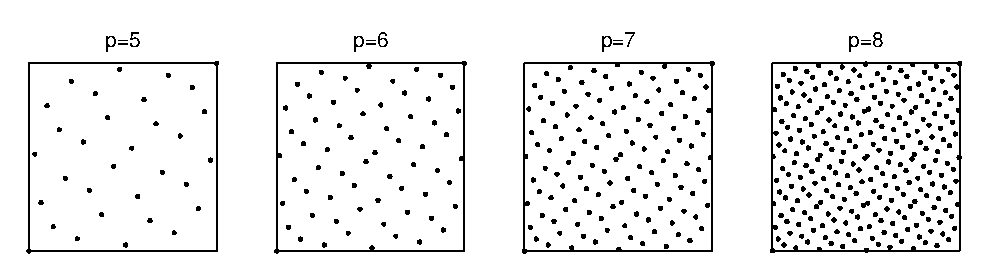
\includegraphics [scale = 0.6]{images/rev-bit-matrix.eps}
    \end{center}
    \caption{Bit inversion matrix}
              \label{fig-rev-bit-matrix}
\end{figure}
The exercise \oldref{exo-bit-reversal} proposes to write a recursive function to perform the bit reversal. Using the \texttt{rev \_bits} procedure allows you to write a \texttt{fft \_dit} function that does not use temporary memory. The end of this procedure replaces the recursive calls with nested \texttt{\pfor} loops. The figure \figref{fig-inversion-bits} shows the operations to perform to reverse the inputs of a vector, highlighting the necessary permutations. \begin{figure}[ht]
    \begin{center}
    \includegraphics [scale = 0.6]{images/inversion-bits.eps}
    \end{center}
    \caption{Inversion of bits by permutation of inputs}
              \label{fig-inversion-bits}
\end{figure}
 
% ------------------------------------------------- -----
% ------------------------------------------------- -----
% sub-section - Frequency decimation                            
% ------------------------------------------------- -----
% ------------------------------------------------- -----
\subsection{Frequency decimation}
\label{sect2-frequency-decimation} 
 
 
\index{Frequency!decimation} We are going to redo the calculations that led to the equations \eqref{eq-danielson-lanczos-a} and \eqref{eq-danielson-lanczos-b}, but this time by performing a grouping according to the frequencies of the transform. The algorithm that we will obtain will be in a way the symmetric of the \guill{classical} algorithm proposed by \nompropre{Cooley} and \nompropre{Tukey}. Even if this new implementation will not improve speed of execution, it is important to have in mind the two dual versions of the FFT, just as it is important to master the temporal and frequency properties of the Fourier transform.
 
 
In accordance with the notations \eqref{eq-part-gd}, we denote by $ f_g $ (resp. $ F_d $) the $ N / 2 $ first entries (resp. $ N / 2 $ last) of the vector $ f $. We have
\begin{equation*}
\wh{f}[k] = \sum_{n = 0}^{N / 2-1}{\left(f_g [n] + e^{- k N / 2 \frac{2 \imath \pi}{N}} f_d [n] \right) e^{- nk \frac{2 \imath \pi}{N}}}.
\end{equation*}
We are therefore led to make a distinction according to the parity of $ k $. By following the notations of the equation \eqref{eq-part-even-odd}, we consider $ (\wh{f} \:)^0 $ (resp. $ (\wh{f} \:)^1 $) the even (resp. odd) part of the transformed vector. Be careful, these vectors should not be confused with $ \wh{f^0} $ and $ \wh{f^1} $, which are the transforms of the vectors $ f^0 $ and $ f^1 $. We therefore write, for $ k \in \{0, \ldots, \, N / 2-1\} $,
\begin{align*}
(\wh{f} \:)^0 [k] & = \wh{f}[2k] = \sum_{n = 0}^{N / 2-1}{\left(f_g [n] + f_d [n] \right) e^{- nk \frac{2 \imath \pi}{N / 2}}} \\
(\wh{f} \:)^1 [k] & = \wh{f}[2k + 1] = \sum_{n = 0}^{N / 2-1}{e^{- k \frac{2 \imath \pi}{N}} \left(f_g [n] - f_d [n] \right) e^{- nk \frac{2 \imath \pi}{N / 2}}}.
\end{align*}
By using the operator $ \Ss_N^x $ introduced in \eqref{eq-operator-S}, we obtain the following recurrence equations:
\begin{align*}
(\wh{f} \:)^0 & = \Ff \left(f_g + f_d \right) \\
(\wh{f} \:)^1 & = \Ff \left(\Ss_{N / 2}^{1/2} (f_g - f_d) \right).
\end{align*}
 
 
 
Contrary to the technique of temporal decimation, we see that the sub-vectors for which we must calculate the Fourier transform are directly obtained from the input vector (just take the left and right parts). On the other hand, the output vector must be composed, according to the parity of the index, either of the values of one transform or of the other. To avoid having to use temporary memory, we will use the same trick as for the temporal decimation, but in the other direction. We will be satisfied with juxtaposing the two transforms, that is to say putting the vectors $ (\wh{f} \:)^0 $ then $ (\wh{f} \:)^1 $. To obtain the correct result, it will suffice, at the end of the procedure, to put the frequencies back in the correct order, by calling the \texttt{rev \_bits} function. We can then write a non-iterative version of the FFT which uses the principle of frequency decimation, it is the procedure \texttt{fft \_dif} which is written in paragraph \ref{listing-fft_dif}.
 
\begin{rem}{(\upshape \textbf{Time and frequency}).} 
We can see that the frequency decimation is exactly symmetrical to the temporal decimation. Acting on the indices of the result vector (i.e. on the frequencies) instead of acting on the indices of the input vector results in a reversal of the bits in the final phase of the algorithm .
\end{rem}
 
 
 
To conclude, we can already notice the wide variety of variations of the FFT algorithm at our disposal. Many other methods will also be described in the following chapters and exercises. The literature revolving around FFT is gigantic, it is undoubtedly one of the most extensive fields of numerical analysis. Review articles have been written, for example by \nompropre{Burrus} \cite{burrus-fft}. The question is therefore to know which is the best method. Of course, there is no definitive answer, because too many factors come into play, not only concerning the length of the transform and the type of data (real, complex, etc.), but above all the type of architecture (machine, operating system, parallel architecture, memory cache, etc.) and the type of precision desired. If in doubt, it is better to stay on a simple, but robust implementation, even if it means sacrificing a little efficiency.
% ------------------------------------------------- -----
% ------------------------------------------------- -----
% sub-section - Matrix writing                            
% ------------------------------------------------- -----
% ------------------------------------------------- -----
\subsection{Matrix writing}
\label{sect1-matrix-writing} 
 
 
\index{Vandermonde!matrix} \index{Unit!matrix} \index{Unitary!endomorphism} \index{Interpolation} If we write the matrix $ \Omega_N $ of the linear operator $ \Ff: \CC^N \rightarrow \CC^N $ in canonical bases, we get
\begin{equation}
\label{eq-defn-matrix-fourier}
\Omega_N \eqdef \begin{pmatrix} 1 & 1 & 1 & \ldots & 1 \\1 & \omega_N^{-1} & \omega_N^{- 2} & \ldots & \omega_N^{- (N- 1)} \\1 & \omega_N^{- 2} & \omega_N^{- 4} & \ldots & \omega_N^{- 2 (N-1)} \\\vdots & \vdots & \vdots & \vdots & \vdots \\1 & \omega_N^{- (N-1)} & \omega_N^{- 2 (N-1)} & \ldots & \omega_N^{- (N-1) (N-1 )} \end{pmatrix}.
\end{equation}
This matrix corresponds to a matrix of \textit{Vandermonde}. These matrices occur when we write the linear system corresponding to the search for the unique polynomial of degree $N$ passing through $N$ distinct points. There is nothing surprising about this, since we will see in Section~\ref{sect1-calculations-products}, that the computation of inverse DFT corresponds to the computation of the coefficients of the interpolation polynomial at points quite particular, the \ordin{N}{th} roots of the unit.
 
 
\label{notation-47} The formula of the inverse Fourier transform \eqref{eq-transforme-fourier-discr-inverse} results in the fact that the inverse of the matrix $ \Omega_N $ is the matrix $ \frac{1}{N} \Omega_N^* $, where we denote by $ M^* \eqdef \transp{\ol{M}} $ the adjoining matrix of $ M $. This means that the matrix $ \frac{1}{\sqrt{N}} \Omega_N $ is unitary, that is to say $ \Omega_N \Omega_N^* = N \Id_N $. The equations of \textit{Danielson-Lanczos} \eqref{eq-danielson-lanczos-a} and \eqref{eq-danielson-lanczos-b} can then be written in the form of a factorization of the matrix $ \Omega_N $:
\begin{equation*}
\Omega_N \begin{pmatrix} a_0 \\\vdots \\a_{N-1} \end{pmatrix} = \begin{pmatrix} \Omega_{N / 2} & \Delta_{N / 2} \Omega_{N / 2} \\\Omega_{N / 2} & - \Delta_{N / 2} \Omega_{N / 2} \end{pmatrix} \begin{pmatrix} a_0 \\\vdots \\a_{N-2 } \\a_1 \\\vdots \\a_{N-1} \end{pmatrix},
\end{equation*}
where we noted $ \Delta_{N / 2} = \diag (1, \, \omega_N^{-1}, \ldots, \, \omega_N^{- (N / 2-1)}) $.

% ------------------------------------------------- -----
% ------------------------------------------------- -----
% ------------------------------------------------- -----
% section - Circular convolution                            
% ------------------------------------------------- -----
% ------------------------------------------------- -----
% ------------------------------------------------- -----
\section{Circular convolution}
% \addcontentsline{toc}{section}{Circular convolution}
\label{sect1-tfd-prod-convol} 
 
\index{Convolution!circular} \index{Group!cyclic} We have defined in paragraph \ref{sect2-convolution-transforme-fourier}, the product of convolution on any abelian group, and we will now apply this definition as well as the convolution theorem \ref{thm-convolution-trans-fourier-grpe-abelien}, in the simple case of a cyclic group, and more precisely by using the language of the discrete Fourier transform which was defined in paragraph \ref{sect1-language-processing-signal}.
% ------------------------------------------------- -----
% ------------------------------------------------- -----
% sub-section - Circular convolution                            
% ------------------------------------------------- -----
% ------------------------------------------------- -----
\subsection{Circular convolution}
\label{sect1-convolution-circular} 
 
\index{Convolution!circular} Let us start by recalling the definition of the convolution product as well as the main results already obtained.
 
\begin{defn}[Discrete convolution product]
\index{Convolution product!discrete} Let $ \{f[n]\}_{n = 0}^{N-1} $ and $ \{g [n]\}_{n = 0}^{N-1} $ two discrete samples (assumed to represent signals sampled at the same times, regularly spaced). We define the convolution product $ f * g $ of the two signals by the equation
\begin{equation}
\label{eq-convolution-discrete}
(f * g) [n] \eqdef \sum_{k = 0}^{N-1}{f[k] g [nk]}, \quad \quad n = 0, \ldots, \, N-1 .
\end{equation}
\end{defn}
 
 
\begin{rem}
In the equation \eqref{eq-convolution-discrete}, the quantity $ nk $ is of course calculated modulo $N$, which amounts to considering the samples $ f $ and $ g $ as periodic functions of period $N$. This formula is the translation of the equation \eqref{eq-formula-prod-convol-grpe-abelien}, in the case of the group $ G = \ZZ/N \ZZ $, taking care to use an additive notation instead of multiplicative notation. From the perspective of a computer implementation, we can give a more explicit formula:
\begin{equation*}
(f * g) [n] \eqdef \sum_{k = 0}^{n}{f[k] g [nk]} + \sum_{k = n + 1}^{N-1}{f[ k] g [n-k + N]}, \quad \quad n = 0, \ldots, \, N-1.
\end{equation*}
\end{rem}
 
 
\begin{prop}
The circular convolution product is commutative, and the mapping $ (f, \, g) \mapsto f * g $ endows $ \CC^N $ with an algebra structure.
\end{prop}
\begin{proof}
The only non-trivial thing to check is the commutativity, which is obtained by making the change of variable $ k'= nk $ in the equation \eqref{eq-convolution-discrete}.
\end{proof}
We can now state the convolution theorem \ref{thm-convolution-trans-fourier-grpe-abelien}, in terms of a discrete Fourier transform.
 
\begin{prop}[Convolution and TFD]
\label{prop-convol-tfd}
Let $ \{f[n]\}_{n = 0}^{N-1} $ and $ \{g [n]\}_{n = 0}^{N-1} $ two discrete samples. We have the convolution formula
\begin{equation}
\label{eq-formula-convolution-tfd}
\forall n \in \{0, \ldots, \, N-1\}, \quad \wh{f * g}[n] = \wh{f}[n] \wh{g}[n].
\end{equation}
\end{prop}
\begin{proofnoqed}
For the explanations to be clearer, we will write $ f_1 $ and $ g_1 $ the functions of $ \ZZ/N \ZZ $ in $ \CC $ associated with the samples $ f $ and $ g $ (which are of size $N$). We then have, for $ n \in \{0, \ldots, \, N-1\} $ (where, in terms of an abelian group, $ n \in \ZZ/N \ZZ $),
\begin{equation}
\label{eq-lien-tfd-trans-fourier}
\wh{f}[n] = \wh{f_1} (\chi_n) \quad \quad \text{et} \quad \quad \wh{g}[n] = \wh{g_1} (\chi_n),
\end{equation}
where we noted $ \{\chi_0, \ldots, \, \chi_{N-1}\} $ the characters, that is to say the elements of the dual $ \wh{\ZZ/N \ZZ} $ (see the equation \eqref{eq-formula-character-znz}). Using the theorem \ref{thm-convolution-trans-fourier-grpe-abelien}, for the functions $ f_1 $ and $ g_1 $ on $ G = \ZZ/N \ZZ $, we obtain
\begin{equation*}
\wh{f_1 * g_1} (\chi_n) = \wh{f_1} (\chi_n) \wh{g_1} (\chi_n).
\end{equation*}
However, we also have
\begin{equation*}
\wh{f * g}[n] = \wh{f_1 * g_1} (\chi_n).
\end{equation*}
This thus makes it possible to write, using the equations \eqref{eq-lien-tfd-trans-fourier},
\begin{equation*}
\wh{f * g}[n] = \wh{f_1} (\chi_n) \wh{g_1} (\chi_n) = \wh{f}[n] \wh{g}[n]. \tag *{\qed}
\end{equation*}
\end{proofnoqed}
 
 
\begin{rem}{(\upshape \textbf{Finite signals and periodization}).} 
\index{Periodization} The main theoretical difficulty of the discrete Fourier transform is the assimilation between our sample $ \{f[n]\}_{n = 0}^{N-1} $ and a function $ f $ set to $ \ZZ/N \ZZ $. This assimilation has the advantage of obtaining algebraic formulas at a lower cost such as the result of inversion \ref{prop-tfd-inverse} as well as that of convolution \ref{prop-convol-tfd}. However, this approach implies that our function $ f $, if we look at it as a signal in time is in fact a periodic function, of period $N$. This goes against the natural intuition which wants us to consider our (finite) signal $ f $ as zero outside the interval in which it is defined. It is on this point that we will have to pay attention when we want to calculate the convolution products between two finite signals. It is precisely this problem which is raised in Paragraph~\ref{sect1-convolution-acyclic} during the study of non-circular convolution.
\end{rem}
 
% ------------------------------------------------- -----
% ------------------------------------------------- -----
% sub-section - Calculation with the FFT                            
% ------------------------------------------------- -----
% ------------------------------------------------- -----
\subsection{Calculation with the FFT}
\label{sect1-convolution-calcul-fft} 
 
A naive implementation of the equation \eqref{eq-convolution-discrete} leads to a number of operations (complex multiplications and additions) of the order of $ O(n^2) $. Indeed, it is necessary to calculate the $N$ values of the convolée, and each time, a sum of $N$ products appears. However, using the convolution formula \eqref{eq-formula-convolution-tfd} and the inversion formula \eqref{eq-transforme-fourier-discr-inverse}, we can write an equation that will turn out to be very useful :
\begin{equation*}
f * g = \Ff^{-1} \left(\wh{f} \cdot \wh{g} \right),
\end{equation*}
where we noted $ f $ and $ g \in \CC^N $ two samples of size $N$. Thanks to the FFT algorithm, the calculation of the transforms $ \wh{f} $ and $ \wh{g} $ can be done in a number of operations of the order of $ O(N \log (N) ) $, and the computation of the product $ \wh{f} \cdot \wh{g} $ requires of course only $N$ complex multiplications. In the end, we thus manage to calculate a convolution product with a number of operations of the order of $ O(N \log (N))$.

% ------------------------------------------------- -----
% ------------------------------------------------- -----
% sub-section - Acyclic convolution                            
% ------------------------------------------------- -----
% ------------------------------------------------- -----
\subsection{Acyclic convolution}
\label{sect1-convolution-acyclic} 
 
 
\index{Convolution!acyclic} We are going to leave for a short time the transformations linked to the group structure of $ \ZZ/N \ZZ $ to define an operation which does not respect this cyclic structure at all, the acyclic convolution (also called linear convolution), denoted $ \star $ (not to be confused with the $ * $ of cyclic convolution). The support of a $ f \in \CC^\ZZ $ signal is defined by
\begin{equation*}
\Supp (f) \eqdef \enscond{n \in \ZZ}{f[n] \neq 0}.
\end{equation*}
We start by defining the acyclic convolution for two signals $ \{f_1 [n]\}_{n \in \ZZ} $ as well as $ \{f_2 [n]\}_{n \in \ZZ} $ whose support is assumed to be finite, which means that $ \Supp (f_1) $ and $ \Supp (f_2) $ are finite sets. We then define the sequence $ f_1 \star f_2 $ by
\begin{equation}
\label{eq-convolution-acyclic}
\forall n \in \ZZ, \quad f_1 \star f_2 [n] = \sum_{k \in \ZZ}{f_1 [k] f_2 [nk]}.
\end{equation}
Note that we have the very useful equation:
\begin{equation*}
\Supp (f_1 \star f_2) \subset \Supp (f_1) + \Supp (f_2) \eqdef \enscond{n + p}{n \in \Supp (f_1), \; p \in \Supp (f_2)}.
\end{equation*}
Linear convolution therefore has nothing to do with cyclic convolution, which is an operation on vectors of $ \CC^N $ (and results in a vector of $ \CC^N $). However, by creating from our two sequences, two vectors $ \wt{f_1} $ and $ \wt{f_2} $ of size $N$ sufficiently large, we will see that we can calculate the non-zero values of $ f_1 \star f_2 $ as some entries of the vector $ \wt{f_1} * \wt{f_2} $.
 
 
\index{Support} Let us start by noticing that the size necessary to store the entries of $ f_1 \star f_2 $ is $ N \eqdef N_1 + N_2 - 1 $, where we have noted $ N_1 $ and $ N_2 $ the sizes supports of $ f_1 $ and $ f_2 $. We can translate the indices of $ f_1 $, which allows us to assume that they are $ \{0, \ldots, \, N_1-1\} $. This implies that we must perform the same translation on the vector $ f $. So let's start by creating a vector $ \wt{f_1} \in \CC^{N} $ by first copying the non-zero $ N_1 $ entries of $ f_1 $, then adding zeros. The construction of the vector $ \wt{f_2} $ is a little more difficult, since it is necessary to take into account the negative indices. Copy the entries with positive indices of $ f_1 $ into $ \wt{f_2} \in \CC^{N} $, then put enough zeros, then copy the entries with negative indices. More precisely, if we write $ \Supp (f_2) = \{- P, \ldots, \, 0, \ldots, \, Q\} $, with $ N_2 = Q + P + 1 $, then we will have
\begin{equation*}
\wt{f_2} \eqdef \{f_2 [0], \, f_2 [1], \ldots, \, f_2 [Q], \, 0, \ldots, \, 0, \, f_2 [-P], \ldots, \, f_2 [-1]\} \in \CC^N.
\end{equation*}
Once all these transformations have been carried out, we can finally write:
\begin{equation*}
\forall n \in \{0, \ldots, \, N_1 + Q-1\}, \quad f_1 \star f_2 [n] = \wt{f_1} * \wt{f_2}[n].
\end{equation*}
For indices located in the interval $ \{- P, \ldots, \, -1\} $, care must be taken because, due to circular convolution, they have been moved in the interval $ \{NP , \ldots, \, N-1\} $. However, in practice (for example, for filtering), we only use the indices $ \{0, \ldots, \, N_1\} $.
 
 
Once this transformation is done, we can of course use the algorithm presented in Section~\ref{sect1-convolution-calcul-fft} to quickly calculate the convolution. This algorithm, which goes hand in hand with the technique of adding zeros that we have just explained, will allow filtering to be carried out quickly. All this will be explained in detail in paragraph \ref{sect1-filtering}. It may be noted that when the size of one of the two vectors is much smaller than that of the other, there is a strategy which makes it possible to avoid adding too many zeros at the end of the shorter vector. This method is exposed to the exercise \oldref{exo-calcul-convolution-fft}.
 
 
In the following, we will often directly consider the linear convolution of two vectors of $ \CC^N $, and in this case, the negative indices will be placed at the end of the vector, (it will therefore be necessary to add zeros between the positive indices and these negative indices to be able to use the FFT algorithm). However, it must be remembered that cyclic and acyclic convolutions give very different results. For example, the figure \figref{fig-diff-conv-linear-circular} shows a comparison of the two convolutions. Filtering by $ g $ performs a kind of \guill{local mean}. For the central values of $ k $, more precisely $ 2 \leq k \leq N-4 $, we have $ f * g [k] = f \star g [k] $. However, for the edge values, we find different results. \begin{figure}[ht]
    \begin{center}
    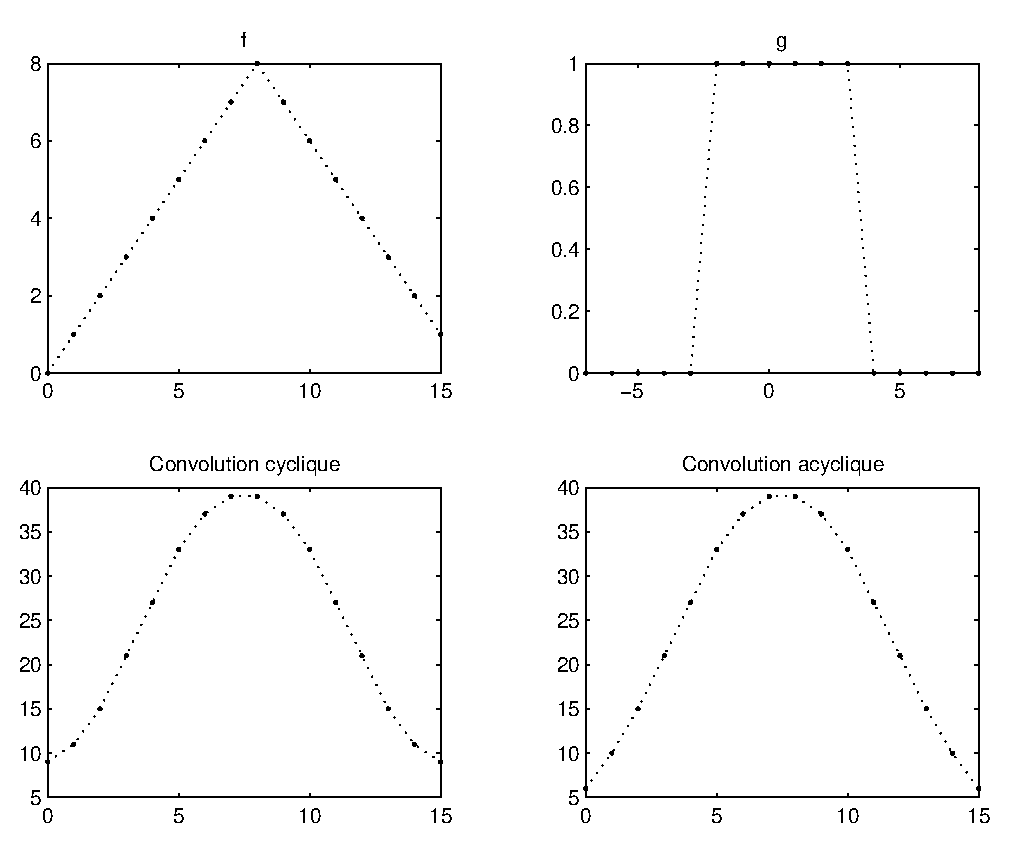
\includegraphics [scale = 0.6]{images/diff-conv-lineaire-circulaire.eps}
    \end{center}
    \caption{Cyclic and acyclic convolutions}
              \label{fig-diff-conv-linear-circular}
\end{figure}
Thus, in the majority of applications where the vector $ x $ will represent a temporal signal, acyclic convolution will be preferred, so as not to alter the values on the edges. All this will be covered in detail when explaining the different types of filtering, in Section~\ref{sect1-filtering}.

% ------------------------------------------------- -----
% ------------------------------------------------- -----
% ------------------------------------------------- -----
% section - In higher dimension                            
% ------------------------------------------------- -----
% ------------------------------------------------- -----
% ------------------------------------------------- -----
\section{In higher dimension}
% \addcontentsline{toc}{section}{In higher dimension}
\label{sect1-tfd-dim-sup} 
 
 
In this paragraph, to simplify the explanations, we will restrict ourselves to calculations of transforms in dimension 2. Generalization to higher dimensions, even if it can be dangerous from the point of view of programming, does not present theoretical difficulties.
% ------------------------------------------------- -----
% ------------------------------------------------- -----
% sub-section - Discrete Fourier transform in 2D                            
% ------------------------------------------------- -----
% ------------------------------------------------- -----
\subsection{Discrete Fourier transform in 2D}
\label{sect2-transforme-discrete-2d} 
 
\index{Fourier transform!in 2D}
 
\begin{defn}[two-dimensional DFT]
A two-dimensional sample is represented by a matrix $ \left\{f[i, \, j] \right\} \in \CC^{N \times P} $. \\The indices are therefore $ i \in \{0, \ldots, \, N-1\} $ and $ j \in \{0, \ldots, \, P-1\} $. Its discrete Fourier transform is a $ N \times P $ matrix defined by
\begin{equation}
\label{eq-defn-tfd-2d}
\wh{f}[k, \, l] \eqdef \sum_{i, \, j}{f[i, \, j] e^{- \frac{2 \imath \pi}{N} ik} e^{- \frac{2 \imath \pi}{P} jl}},
\end{equation}
where $ k \in \{0, \ldots, \, N-1\} $ and $ l \in \{0, \ldots, \, P-1\} $.
\end{defn}
As for the one-dimensional case, we can still make the link with the Fourier transform on an abelian group, by considering the group $ G \eqdef \ZZ/N \ZZ \times \ZZ/P \ZZ $. The characters in this group are $ \chi_{ij} $, for $ 0 \leq i <N $ and $ 0 \leq j <P $, defined by
\begin{equation*}
\forall (n, p) \in \ZZ/N \ZZ \times \ZZ/P \ZZ, \quad \chi_{ij} (n, p) \eqdef \left(\omega_N \right)^{- in } \left(\omega_P \right)^{- jp}.
\end{equation*}
We can therefore translate the equation \eqref{eq-defn-tfd-2d} by
\begin{equation*}
\forall k \in \{0, \ldots, \, N-1\}, \; \forall l \in \{0, \ldots, \, P-1\}, \quad \wh{f}[k, \, l] = \wh{f} (\chi_{kl}),
\end{equation*}
where we noted $ f $ both the sample and the associated function $ f: G \rightarrow \CC $.
 
\index{Isomorphism} Once again, we see that the function
\begin{equation*}
\Ff: \func{\CC^{N \times P}}{\CC^{N \times P}}{f}{\Ff(f) = \wh{f}}
\end{equation*}
is an algebra isomorphism of which we explicitly know the reverse.
 
\begin{prop}[2D inversion formula]
Let $ f \in \CC^{N \times P} $ be a 2D sample of size $ N \times P $. We have the inversion formula
\begin{equation*}
f[i, \, j] = \frac{1}{NP} \sum_{k, \, l}{\wh{f}[k, \, l] e^{\frac{2 \imath \pi }{N} ik} e^{\frac{2 \imath \pi}{P} jl}},
\end{equation*}
for $ i \in \{0, \ldots, \, N-1\} $ and $ j \in \{0, \ldots, \, P-1\} $.
\end{prop}
 
 
 
The important point is of course whether we still have a fast algorithm to calculate the DFT in dimension two. The answer is given by a simple rewrite of the equation \eqref{eq-defn-tfd-2d}, for $ k \in \{0, \ldots, \, N-1\} $ and $ l \in \{0, \ldots, \, P-1\} $:
\begin{equation*}
\wh{f}[k, \, l] = \sum_{i = 0}^{N-1}{\left(\sum_{j = 0}^{P-1}{f[i, \, j] e^{- \frac{2 \imath \pi}{P} jl}} \right) e^{- \frac{2 \imath \pi}{N} ik}} = \sum_{i = 0 }^{N-1}{\wh{F_i}[l] e^{- \frac{2 \imath \pi}{N} ik}},
\end{equation*}
where we denote by $ F_i \in \CC^P $ the vector formed by the \ordin{i}{ith} row of the matrix $ f $, and $ \wh{F_i} $ its one-dimensional DFT.
 
 
To calculate the TFD in 2D of a $ f $ matrix, it is therefore sufficient to calculate the TFD of each of its rows, then to calculate the TFD of the columns of the matrix obtained. In a more synthetic way, we can write matricially:
\begin{equation*}
\wh{f} = \transp{\Ff_{\text{1D}} \left(\transp{\Ff_{\text{1D}} (f)} \right)},
\end{equation*}
where the operator $ \Ff_{\text{1D}} $ performs the one-dimensional DFT on the rows of a matrix. It is also possible to carry out the calculations in the reverse direction, that is to say first calculate the transform on the columns, then on the rows. Matrix, like $ \transp{\Omega_N} = \Omega_N $, the transformation equation is written $ \wh{f} = \Omega_N f \Omega_P $, where $ \Omega_N $ is defined at the equation \eqref{eq-defn-matrix-fourier}.
 
 
\index{Oscillation} Figure \figref{fig-tfd-2d} shows the 2D Fourier transform of an image, which is just another way of representing a 2D sample (the values of the function are represented by levels gray, varying from black for 0 to white for 1). We can intuitively interpret the spectrum obtained. The value of $ \wh{f}[i, \, j] $, which we can \guill{read} directly on the image representing the spectrum, corresponds to a certain amount of(two-dimensional) oscillations present in the image. Please note, for the Fourier transform (right image), the large coefficients are shown in black. These oscillations are characterized by a frequency, $ \frac{1}{N} \sqrt{i^2 + j^2} $, and a direction, that of the vector $ (i, \, j) $. 
	\begin{figure}[ht]
    \begin{center}
    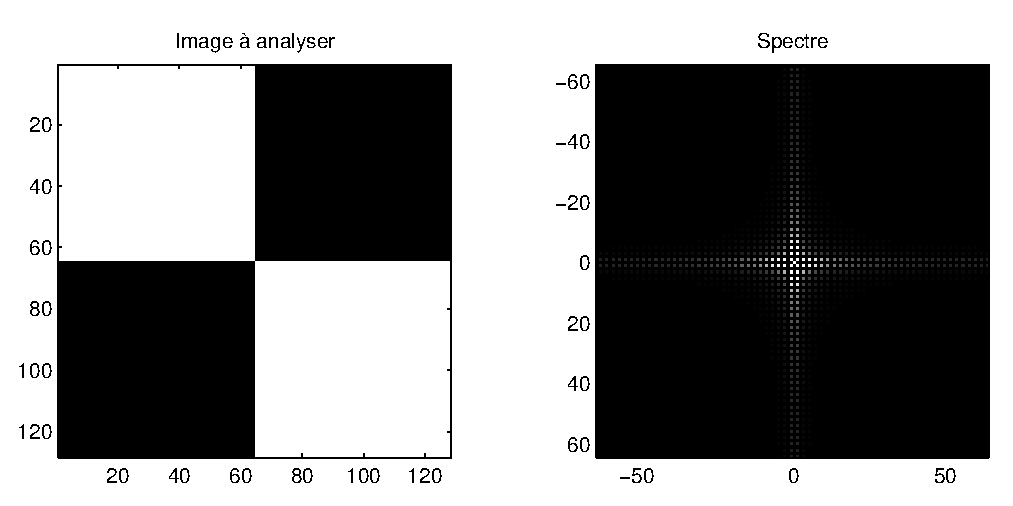
\includegraphics [scale = 0.6]{images/tfd-2d.eps}
    \end{center}
    \caption{2D Fourier transform}
              \label{fig-tfd-2d}
\end{figure}
 
% ------------------------------------------------- -----
% ------------------------------------------------- -----
% sub-section - 2D Convolution                            
% ------------------------------------------------- -----
% ------------------------------------------------- -----
\subsection{2D convolution}
\label{sect2-convolution-2d} 
 
 
\index{Convolution!2D} The convolution between two two-dimensional signals is a direct generalization of the cyclic convolution described in Section~\ref{sect1-convolution-circular}. Once again, we can keep in memory the definition of convolution over a finite group (defined in paragraph \ref{sect2-convolution-transforme-fourier}). This is of course to consider the group $ G \eqdef \ZZ/N \ZZ \times \ZZ/P \ZZ $. We can then interpret the functions of $ \CC [G] $ as images of size $ N \times P $, which we would have extended by periodicity along the two axes. Here is the definition of convolution between two two-dimensional signals. We check that this is an immediate translation of the definition given in the framework of finite abelian groups.
 
\begin{defn}[Two-dimensional convolution]
Let $ f $ and $ g $ be two samples of size $ N \times P $. We define their cyclic convolution product $ f * g $, which is a matrix of size $ N \times P $, as follows:
\begin{equation}
\label{eq-defn-product-convol-2d}
(f * g) [i, \, j] \eqdef \sum_{k = 0}^{N-1}{\sum_{l = 0}^{P-1}{f[k, \, l] g [ik, \, jl]}},
\end{equation}
for $ i \in \{0, \ldots, \, N-1\} $ and $ j \in \{0, \ldots, \, P-1\} $. Of course, all the operations on the indices must be carried out modulo $N$ (resp. $ P $) for the indices on the left (resp. On the right).
\end{defn}
 
 
 
A naive calculation of the convolution product directly by the formula \eqref{eq-defn-product-convol-2d} requires $ (NP)^2 $ operations. In order to quickly calculate such a product, it is necessary to use the algebra morphism property of the Fourier transform on a finite group, which is recalled here in the context of the 2D Fourier transform.
 
\begin{prop}[2D and TFD convolution]
\label{prop-convol-tfd-2d}
Let $ f $ and $ g $ be two samples of size $ N \times P $. We have the convolution formula
\begin{equation}
\label{eq-formula-convolution-tfd-2d}
\forall i \in \{0, \ldots, \, N-1\}, \; \forall j \in \{0, \ldots, \, P-1\}, \quad \wh{f * g}[i, \, j] = \wh{f}[i, \, j] \wh{g}[i, \, j].
\end{equation}
\end{prop}
\begin{proof}
The proof is the exact copy of that of the proposition \ref{prop-convol-tfd}. It is simply necessary to change the cardinal of the group (which is worth $ NP $ and no longer $N$), and to use an indexing adapted for the characters and the indices of the samples, i.e. $ i \in \{0, \ldots, \, N-1\} $ and $ j \in \{0, \ldots, \, P-1\} $.
\end{proof}
This theorem suggests, in order to calculate a convolution, to use the technique to which we are starting to be accustomed. First, you have to calculate the DFTs of the two signals you want to combine. Then, we must multiply them point to point, and finally calculate the inverse transform of the signal obtained. Be careful with the fact that to implement this algorithm, it is necessary to move the entries of negative indices in the two signals, so as to have a signal $N$ periodic on the abscissas, $ P $ periodic on the ordinates, and with indices $ (i, \, j) $ such as $ i \in \{0, \ldots, \, N-1\} $ and $ j \in \{0, \ldots, \, P-1\} $.
 
 
We will see in paragraph \ref{sect2-filtering-2d}, where we will talk about 2D filtering, what are the \guill{intuitive} properties of cyclic convolution, as well as immediate applications to image analysis. We can however give an example of convolution on functions represented by their graph in 3D. Thus the figure \figref{fig-convolution-2d} represents an irregular $ f $ function that we have convolated with a $ g $ function having the shape of a bump (and integral equal to $ 1 $). Convolution has a regularization effect since it realizes a weighted average of the original function in the neighborhood of each point. \begin{figure}[ht]
    \begin{center}
    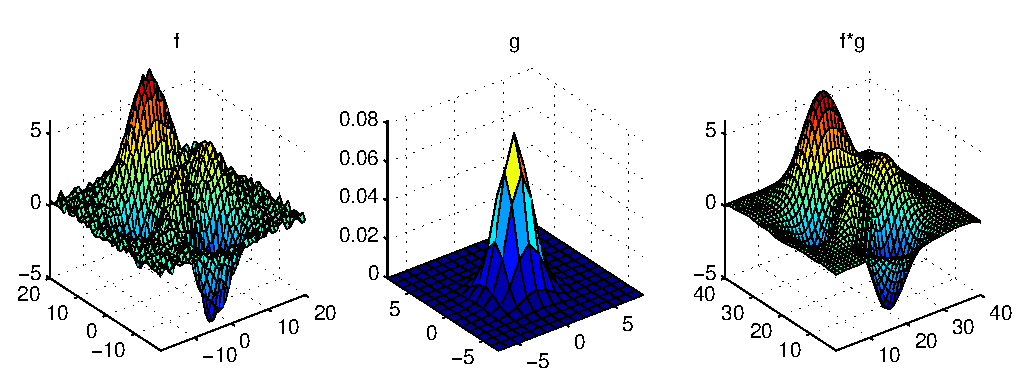
\includegraphics [scale = 0.8]{images/convolution-2d.eps}
    \end{center}
    \caption{2D Convolution}
              \label{fig-convolution-2d}
\end{figure}
 
% ------------------------------------------------- -----
% ------------------------------------------------- -----
% ------------------------------------------------- -----
% section - Symmetry and discrete transform                            
% ------------------------------------------------- -----
% ------------------------------------------------- -----
% ------------------------------------------------- -----
\section{Symmetry and discrete transform}
% \addcontentsline{toc}{section}{Symmetry and discrete transform}
\label{sect1-symetrie-tfd} 
 
\index{Symmetry} In this paragraph, we will give some additional properties of the discrete Fourier transform, and thus create its eigenvectors from given vectors.
% ------------------------------------------------- -----
% ------------------------------------------------- -----
% sub-section - Symmetry properties                            
% ------------------------------------------------- -----
% ------------------------------------------------- -----
\subsection{Symmetry properties}
\label{sect2-prop-symmetry} 
 
Let's start by defining different operations on the functions of $ \ZZ/N \ZZ $ in $ \CC $.
 
\begin{defn}[Symmetry operator]
\label{defn-symmetry-operator}
\index{Operator!of symmetry} \label{notation-48} Let $ f = \{f[0], \ldots, \, f[N-1]\} $ be a vector of size $N$ which we associates a periodic function $ f_1 $, which can be seen as a function $ f_1: \ZZ/N \ZZ \rightarrow \CC $. We define \textit{the symmetrized function} $ f^\sharp $ by:
\begin{equation}
\label{eq-defn-symmetrical-sample}
\forall n \in \{0, \ldots, \, N-1\}, \quad f^\sharp [n] \eqdef f_1 (-n).
\end{equation}
Thus, we have $ f^\sharp = \{f[0], \, f[N-1], \, f[N-2], \ldots, \, f[1]\} $. \\A vector $ f $ is said to be \textit{symmetric} if it satisfies $ f^\sharp = f $. It says \textit{anti-symmetric} if $ f^\sharp = -f $.
\end{defn}
 
 
\begin{defn}[Decomposition]
\label{defn-parts-sym-anti-sym}
\index{Symmetric part} \label{notation-49} For $ f \in \CC^N $, we denote by $ \psym{f} $ and $ \pasym{f} $ the parts \textit{symmetric} and \textit{anti-symmetric} of $ f $, defined by the equations
\begin{align*}
\psym{f} & \eqdef \frac{1}{2} \left(f + f^\sharp \right), \\
\pasym{f} & \eqdef \frac{1}{2} \left(f - f^\sharp \right).
\end{align*}
We have of course the decomposition $ f = \psym{f} + \pasym{f} $.
\end{defn}
 
 
\begin{prop}[Symmetry properties]
Let $ f \in \CC^N $ be a sample. We have the following properties. \begin{itemize}
\item [{\upshape (i)}] $ \Ff(f^\sharp) = N \Ff^{-1} (f) $ as well as $ \Ff^2 (f^\sharp) = N f $ .
\item [{\upshape (ii)}] If $ f $ is symmetric, then $ \Ff^2 (f) = N f $ and $ \Ff(f) $ is symmetric.
\item [{\upshape (iii)}] If $ f $ is anti-symmetric, then $ \Ff^2 (f) = -N f $ and $ \Ff(f) $ is anti-symmetric.
\item [{\upshape (iv)}] If $ f \in \RR^N $ is symmetric, then $ \Ff(f) \in \RR^N $.
\item [{\upshape (v)}] If $ f \in \RR^N $ is anti-symmetric, then $ \Ff(f) \in (\imath \RR)^N $.
\end{itemize}
\end{prop}
\begin{proofnoqed}
We prove (i) and (iv): \\For (i), we have
\begin{equation*}
\Ff(f^\sharp) = \sum_{k \neq 0}{f[-k] \omega_N^{- kn}} + f[0] = \sum_{k = 0}^{N-1}{f[k] \omega_N^{kn}} = \Ff(f) [n].
\end{equation*}
For (iv), if we denote by $ \ol{z} $ the conjugate of $ z \in \CC $, we have
\begin{equation*}
\ol{\Ff(f) [n]} = \sum_{k}{\ol{f[k]} e^{+ \frac{2 \imath \pi}{N} kn}} = \sum_{k}{f^\sharp [k] e^{\frac{2 \imath \pi}{N} kn}} = \Ff(f^\sharp) [n] = \Ff(f) [n]. \tag *{\qed}
\end{equation*}
\end{proofnoqed}
 
% ------------------------------------------------- -----
% ------------------------------------------------- -----
% sub-section - Eigenvalues of the TFD                            
% ------------------------------------------------- -----
% ------------------------------------------------- -----
\subsection{Eigenvalues of the TFD}
\label{sect2-eigenvalues-tfd} 
 
\index{Unit!Matrix} The study of a linear operator is greatly facilitated by the knowledge of its eigenvalues and the associated eigenvectors. Although the $ \frac{1}{\sqrt{N}} \Omega_N $ matrix is arguably the most important unit matrix, finding its eigenvectors is a difficult subject. We will now give a simple way to construct eigenvectors of the DFT.
 
\begin{thmdefn}
\index{Eigenvector} \index{Eigenvalue} Let $ f \in \CC^N $ be a sample. We define
\begin{align*}
& \Uu_+ (f) \eqdef \sqrt{N} \psym{f} + \Ff(\psym{f}) \quad \quad \text{and} & \Uu_- (f) \eqdef \sqrt{N} \psym{f} - \Ff(\psym{f}) \\
& \Vv_+ (f) \eqdef \sqrt{N} \pasym{f} + \imath \Ff(\pasym{f}) \quad \quad \text{and} & \Vv_- (f) \eqdef \sqrt{N} \pasym{f} - \imath \Ff(\pasym{f}).
\end{align*}
We then have
\begin{align*}
& \Ff(\Uu_+ (f)) = \sqrt{N} \Uu_+ (f) \quad \text{et} \quad \Ff(\Uu_- (f)) = - \sqrt{N} \Uu_- (f) \\
& \Ff(\Vv_+ (f)) = - \imath \sqrt{N} \Vv_+ (f) \quad \text{et} \quad \Ff(\Vv_- (f)) = \imath \sqrt{N} \Vv_- (f).
\end{align*}
This means that the vectors $ \Uu_+ (f) $, $ \Uu_- (f) $, $ \Vv_+ (f) $ and $ \Vv_- (f) $ are \textit{eigenvectors} of the discrete Fourier transform.
\end{thmdefn}
\begin{proof}
Let's prove the first equality: $ \Ff(\Uu_+ (f)) = \sqrt{N} \Ff(\psym{f}) + \Ff^2 (\psym{f}) $. And since $ \psym{f} $ is symmetric, we have $ \Ff^2 (\psym{f}) = N \psym{f} $, hence the result.
\end{proof}
 
 
\begin{rem}
We can add that the \textit{eigenvalues} that we have just found are the only ones, since the Fourier transform satisfies $ \Ff^4 (f) = N f $. So its eigenvalues are necessarily \ordin{4}{th} roots of $ N^2 $.
\end{rem}
\index{Eigenvector} \index{Eigenvalue} \index{Fourier transform!partial} \index{Operator square root} Figure \figref{fig-square-root-tfd} shows the different constructed eigenvectors from the function that can be seen on the left of the figure \figref{fig-root-interm-tfd} (that is to say for $ \lambda = 0 $). \begin{figure}[ ht] 
    \begin{center}
    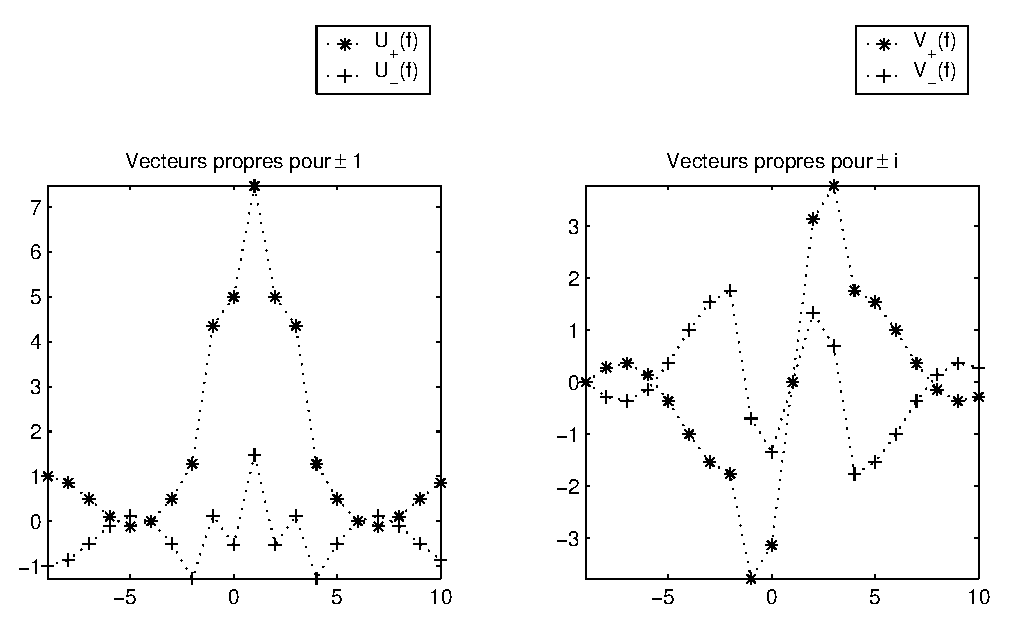
\includegraphics [scale = 0.6]{images/racine-carree-tfd.eps}
    \end{center}
    \caption{Eigenvectors $ \Uu_+ (f), \, \Uu_- (f), \, \Vv_+ (f) $ and $ \Vv_- (f) $}
              \label{fig-square-root-tfd}
\end{figure}
This proposition allows an interesting construction, simply by writing the decomposition of a vector $ f \in \CC^N $ as a function of the eigenvectors of the Fourier transform:
\begin{equation*}
f = \Uu_+ (f) + \Uu_- (f) + \Vv_+ (f) + \Vv_- (f).
\end{equation*}
This allows to consider the operator $ \sqrt{\Ff} $ defined as follows:
\begin{equation*}
\sqrt{\Ff} (f) \eqdef N^{1/4} \Uu_+ (f) + \imath N^{1/4} \Uu_- (f) + (- \imath)^{1 / 2} N^{1/4} \Vv_+ (f) + \imath^{1/2} N^{1/4} \Vv_- (f),
\end{equation*}
where we have chosen for $ \imath^{1/2} $ a \textit{square root} of $ \imath $ (arbitrary choice).
 
We then have $ \sqrt{\Ff} \circ \sqrt{\Ff} = \Ff $: the operator $ \sqrt{\Ff} $ is a square root of the discrete Fourier transform. Likewise, for $ \lambda \in \RR $, we can thus construct $ \Ff^\lambda $, a \ordin{\lambda}{ième} transform of $ \Ff $ (again, the construction n' is absolutely nothing canonical). Figure \figref{fig-root-interm-tfd} shows different intermediate transforms. For $ \lambda = 0.5 $ we get $ \sqrt{\Ff} $. \begin{figure}[ht]
    \begin{center}
    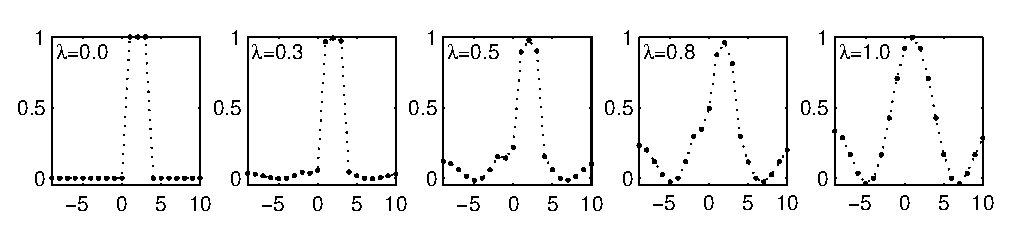
\includegraphics [scale = 0.7]{images/racine-interm-tfd.eps}
    \end{center}
    \caption{Intermediate transformed vectors $ \Ff^\lambda (f) $ for $ \lambda \in [0,1] $}
              \label{fig-root-interm-tfd}
\end{figure}
The exercise \oldref{exo-transforme-partial-fourier} allows to handle a \textit{partial Fourier transform}, which generalizes the construction that we have just performed. We can see, thanks to the example of a Gaussian, that these manipulations correspond to very intuitive notions. For more information on the partial Fourier transform (continuous as well as discrete), one can consult the article of \nompropre{Cariolaro} \cite{cariolaro-partial-fourier}. Finally, the exercise \oldref{exo-diagonalization-tfd} proposes a method to canonically diagonalize the matrix of the TFD.

% ------------------------------------------------- -----
% ------------------------------------------------- -----
% ------------------------------------------------- -----
% section - Exercises                            
% ------------------------------------------------- -----
% ------------------------------------------------- -----
% ------------------------------------------------- -----
\section{Exercises}
% \addcontentsline{toc}{section}{Exercises}
\label{sect1-chap2-exercises} 
 
 
 
\begin{exo}[Bit inversion]
\label{exo-bit-reversal}
 
\index{Bit inversion} We define, for $ n \geq 0 $, vectors $ u^{(n)} $ of size $ 2^n $, by $ u^{(0)} = \{0\} $ and
\begin{equation*}
\forall n> 0, \; \forall k \in \{0, \ldots, \, 2^n-1\}, \quad u^{(n)}[k] \eqdef \left\{\begin{array}{ll} 2 u^{(n-1)}[k] & \text{si} k <2^{n-1} \\2 u^{(n-1)}[k-2^{n-1}] + 1 & \text{si} k \geq 2^{n-1} \end{array} \right. .
\end{equation*}
\begin{enumerate}
\item Calculate the value of $ u^{(n)} $ for $ n = 1, \, 2, \, 3 $.
\item Show that $ u^{(n)} $ is in fact the sequence $ 0, \ldots, \, 2^n-1 $, classified by considering the reverse binary writes of the inputs.
\item Let $ f $ be a vector of size $ 2^n $. We denote by $ \wt{f} $ the sequence determined by
\begin{equation*}
\forall k \in \{0, \ldots, \, 2^n-1\}, \quad \wt{f}[k] \eqdef f[u^{(n)}[k]].
\end{equation*}
What is the use of $ \wt{f} $ when computing the discrete Fourier transform of $ f $?
\item We denote by $ f^0 $ and $ f^1 $ the even and odd parts of $ f $. We denote by $ \wt{f}_d $ and $ \wt{f}_g $ the left and right parts of $ \wt{f} $. What relation binds all these vectors?
\item \index{Matlab@\Matlab{}} \index{Complexity} Implement in \Matlab{} a recursive algorithm to calculate $ \wt{f} $. Compare its complexity to that of the \texttt{\upshape rev \_bits} procedure.
\end{enumerate}
\end{exo}
 
 
\begin{exo}[Good-Thomas algorithm]
\label{exo-algo-good-thomas}
 
\index{Good-Thomas@\nompropreindex{Good-Thomas}} \index{Cooley-Tukey@\nompropreindex{Cooley-Tukey}} \index{Algorithm!of Good-Thomas} We saw in paragraph \ref{sect2-transfo-cooley-tukey} that the FFT algorithm of \textit{Cooley-Tukey} generalized without problem if we had an adequate factorization of $N$, the size of the transformed vector. In this exercise, we will see that if some integers of this factorization are coprime, we can design an even faster algorithm. \begin{enumerate}
\item \index{Ring} \index{Ring!morphism} \index{Chinese!lemma} We assume that $ N = p \, q $ where $ p $ and $ q $ are two prime numbers to each other. We recall the \textit{Chinese lemma}, which says that the application
\begin{equation*}
\varphi \func{\ZZ/N \ZZ}{\ZZ/p \ZZ \times \ZZ/q \ZZ}{n}{(n \mod p, \, n \mod q)}
\end{equation*}
is an isomorphism of rings. Explain the inverse morphism $ \psi $.
\item Let $ f \in \CC^N $. We then define a 2D signal:
\begin{equation*}
\forall k_1 \in \{0, \ldots, \, p-1\}, \; \forall k_2 \in \{0, \ldots, \, q-1\}, \quad F [k_1, \, k_2] \eqdef f[\psi (k_1, \, k_2)].
\end{equation*}
Show that we have
\begin{equation*}
\wh{f}[(s_1 q + s_2 p) \mod N] = \wh{F}[s_1, \, s_2].
\end{equation*}
 
\item Show that when $ s_1 $ traverses $ \{0, \ldots, \, p-1\} $ and $ s_2 $ traverses $ \{0, \ldots, \, q-1\} $, then $ ( s_1 q + s_2 p) \mod N $ iterates $ \{0, \ldots, \, N-1\} $. Deduce how we can calculate the Fourier transform of $ f $ from that of $ F $, by explaining the change of indices.
\item What is the gain compared to a step of the classic FFT algorithm? In particular, what becomes of the operator $ \Ss_N^x $ introduced to the equation \eqref{eq-operator-S}? Propose a recursive procedure which, following the factorization of $N$ obtained at each step, calls the optimal DFT calculation procedure. In addition to the FFT procedures of Cooley-Tukey and Good-Thomas, we can include the Chirp procedure described in the exercise \oldref{exo-chirp-transform-finis-corps}, which is interesting when $ N-1 $ is a Prime number.
\end{enumerate}
\end{exo}
 
 
\begin{exo}[Split-Radix algorithm]
\label{exo-algo-split-radix}
 
\index{Algorithm!split-radix} \index{Split-radix} \index{Twiddle factor} \index{Decimation!frequency} We saw in paragraph \ref{sect2-variations-fft} that it was possible to extend the Cooley-Tukey dichotomy method to compute DFTs of length $ p^r $, by grouping inputs by packets of size $ p $. In this exercise, we will show how, by cleverly choosing packets of varying sizes, we can reduce the number of operations. This choice starts from the observation that the Cooley-Tukey algorithm spends a lot of time calculating the operator $ \Ss_N^x $, whereas for some values of $N$ (for example $ 2 $ or $ 4 $), this last is trivial. In Anglo-Saxon literature, the roots of the unit added by this operator are called \guill{twiddle factors} (literally, \guill{twiddling their thumbs}). We can compare this approach with that of the Good-Thomas algorithm, exercise \oldref{exo-algo-good-thomas}, which in the context of a certain factorization of $N$, eliminates the operator $ \Ss_N^x $. \begin{enumerate}
\item We consider a frequency decimation scheme. Assume that $N$ is a power of $ 2 $. It is recalled that the classical DIF algorithm organizes the following grouping:
\begin{align*}
\enscond{\wh{f}[k]}{k = 0, \ldots, \, N-1} = & \enscond{\wh{f}[2 k]}{k = 0, \ldots, \, \ofrac{N}{2}-1} \bigcup \\
& \enscond{\wh{f}[2 k + 1]}{k = 0, \ldots, \, \ofrac{N}{2}-1}.
\end{align*}
Explain why there is no interest in touching the first part of this grouping. Regarding the second part, we propose the grouping corresponding to base 4 transforms, that is to say:
\begin{align*}
\enscond{\wh{f}[2 k + 1]}{k = 0, \ldots, \, \ofrac{N}{2}-1} = & \enscond{\wh{f}[4 k + 1]}{k = 0, \ldots, \, \ofrac{N}{4}-1} \bigcup \\
& \enscond{\wh{f}[4 k + 3]}{k = 0, \ldots, \, \ofrac{N}{4} -1}
\end{align*}
Show that this leads to the following transformation formulas:
\begin{equation*}
\wh{f}[4k + 2j + 1] = \sum_{n_1 = 0}^{\frac{N}{4} -1}{\omega_{N / 4}^{- k n_1} \omega_N^{-n_1 (2j + 1)} \sum_{n_2 = 0}^{3}{f \left[n_1 + n_2 \ofrac{N}{4} \right] \omega_4^{- n_2 (2j + 1) }}},
\end{equation*}
for $ j = 0, \, 1 $ and $ k = 0, \ldots, \, \frac{N}{4} -1 $. Are domestic sums complicated to calculate? Identify the \guill{twiddle factors}.
\item Find other grouping schemes. Why is grouping by 4 advantageous? Calculate the number of operations required each time, and compare with that of the classic DIF diagram, in base 2.
\item Transform the algorithms described above to obtain a temporal decimation scheme (grouping of inputs). Describe an iterative implementation of the algorithms, not forgetting the bit reversal procedures allowing to save temporary memories.
\end{enumerate} For more information, and a generalization to DFTs of length $ p^r $, we can consult{\upshape \cite{vetterli-split-radix}}.
\end{exo}
 
 
\begin{exo}[Optimized convolution]
\label{exo-calcul-convolution-fft}
 
\index{Convolution!acyclic} We want to compute the acyclic convolution of two finite sequences $ f $ and $ g $ of respective sizes $N$ and $ M $. Assume that $ M $ is much smaller than $N$. For simplicity, suppose that the indices of the two sequences start at $ 0 $. \begin{enumerate}
\item We take $ N = p M $. We denote by $ f_j \eqdef \{f[k + j M]\}_{k = 0}^{M-1} $, for $ j = 0, \, \ldots, \, p -1 $. Show that we have
\begin{equation*}
f \star g [k] = \sum_{j = 0}^{p-1}{f_j \star g [k - j M]}.
\end{equation*}
 
\item \index{Complexity} Deduce a quick way to calculate $ f \star g $ without having to add $ NM-1 $ zeros at the end of $ g $. What is the complexity of the algorithm obtained?
\item If $N$ is not a multiple of $ M $, what can be done?
\end{enumerate}
\end{exo}
 
 
\begin{exo}[Circulating matrix]
\label{exo-circulating-matrix}
 
\index{Matrix!circulating} \index{Determinant!circulating} This exercise has strong similarities with the exercise \oldref{exo-determinant-circulating} on circulating determinants, with a presentation this time using the convolution product. Let $ c \eqdef \transp{(c_0, \ldots, \, c_{N-1})} \in \CC^N $ be a vector of size $N$. We define the circulating matrix $ C $ which is associated with this vector by
\begin{equation*}
C \eqdef \begin{pmatrix} c_0 & c_{N-1} & c_{N-2} & \ldots & c_{1} \\c_1 & c_0 & c_1 & \ldots & c_{2} \\\vdots & \vdots & \vdots & & \vdots \\c_{N-1} & c_{N-2} & c_{N-3} & \ldots & c_{0} \end{pmatrix}.
\end{equation*}
\begin{enumerate}
\item Let $ \{e_1, \ldots, \, e_N\} $ be the canonical basis of $ \CC^N $. We consider the matrix $ R $ whose columns are $ \{e_2, \, e_3, \ldots, \, e_N, \, e_1\} $. We recall that $ \Omega_N $ designates the Fourier matrix, which is defined by the equation \eqref{eq-defn-matrix-fourier}. Show that we have
\begin{equation*}
\Omega_N R \Omega_N^{-1} = D \quad \quad \text{with} \quad D = \diag (1, \, \omega_N^{-1}, \ldots, \, \omega_N^{- (N-1)}).
\end{equation*}
 
\item Show while we have
\begin{equation*}
\Omega_N C \Omega_N^{-1} = \Delta \quad \quad \text{with} \quad \Delta = \diag (\wh{c}[0], \, \wh{c}[1], \ldots, \, \wh{c}[N-1]).
\end{equation*}
Deduce that for $ x \in \CC^N $, we can calculate the product $ C x $ as follows:
\begin{equation*}
C x = \Omega_N^{-1} \left((\Omega_N c) \cdot (\Omega_N x) \right),
\end{equation*}
where we denote by $ \cdot $ the product component by component of the matrices.
\item Show that for $ x \in \CC $, we have $ C x = c * x $. Using the convolution theorem \ref{prop-convol-tfd}, deduce an immediate proof of the previous question.
\end{enumerate}
\end{exo}
 
 
\begin{exo}[Trigonometric interpolation]
\label{exo-interpolation-trigonometric}
\index{Interpolation!trigonometric} \index{Zero padding} Let $ f \in \CC^N $ be a sample of size $ N = 2N_0 + 1 $. We define a vector $ f_0 $ of size $ P = \eta N $ (with $ \eta \in \NN $ sufficiently large) as follows:
\begin{equation*}
\wh{f_0} \eqdef \eta \left\{\wh{f}[0], \, \wh{f}[1], \ldots, \, \wh{f}[N_0], \, 0 , \ldots, \, 0, \, \wh{f}[N_0 + 1], \ldots, \, \wh{f}[N-1] \right\}.
\end{equation*}
Show that we have
\begin{equation*}
\forall k \in \{0, \ldots, \, N-1\}, \quad f[k] = f_0 [\eta k].
\end{equation*}
Deduce a fast algorithm to interpolate a function by trigonometric polynomials. We can see this algorithm in action in figure \figref{fig-fft-interpolation}. \begin{figure}[ht]
    \begin{center}
    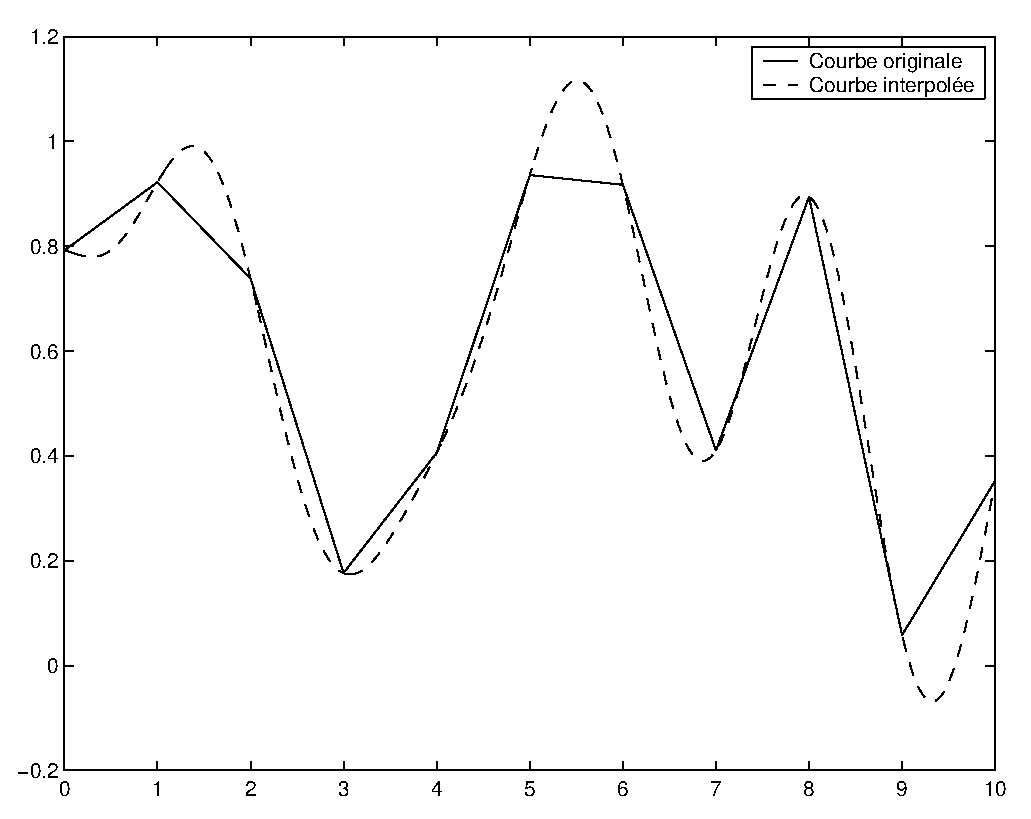
\includegraphics [scale = 0.4]{images/fft-interpolation.eps}
    \end{center}
    \caption{Trigonometric interpolation}
              \label{fig-fft-interpolation}
\end{figure}f
\end{exo}
 
 
\begin{exo}[Chebyshev interpolation]
\label{exo-interpolation-chebyshev}
\index{Chebyshev@\nompropreindex{Chebyshev}} \index{Polynomial!of Chebyshev} \index{Transform!into cosine} \index{Runge phenomenon} \index{Interpolation!of Chebyshev} \index{Interpolation!of Lagrange} \index{Lissajou curve} We define the polynomials of \textit{Chebyshev} by
\begin{equation*}
T_k (X) \eqdef \cos (k \arccos (X)).
\end{equation*}
The figure \figref{fig-polynomes-chebyshev} shows the graphical representations of the polynomials $ T_k $ for small values of $ k $. These are special cases of Lissajou figures (which are used to study wave phenomena), i.e. parameterized curves of the type $ (x = a \cos (kt + c), \, y = b \cos (t)) $. \begin{figure}[ht]
    \begin{center}
    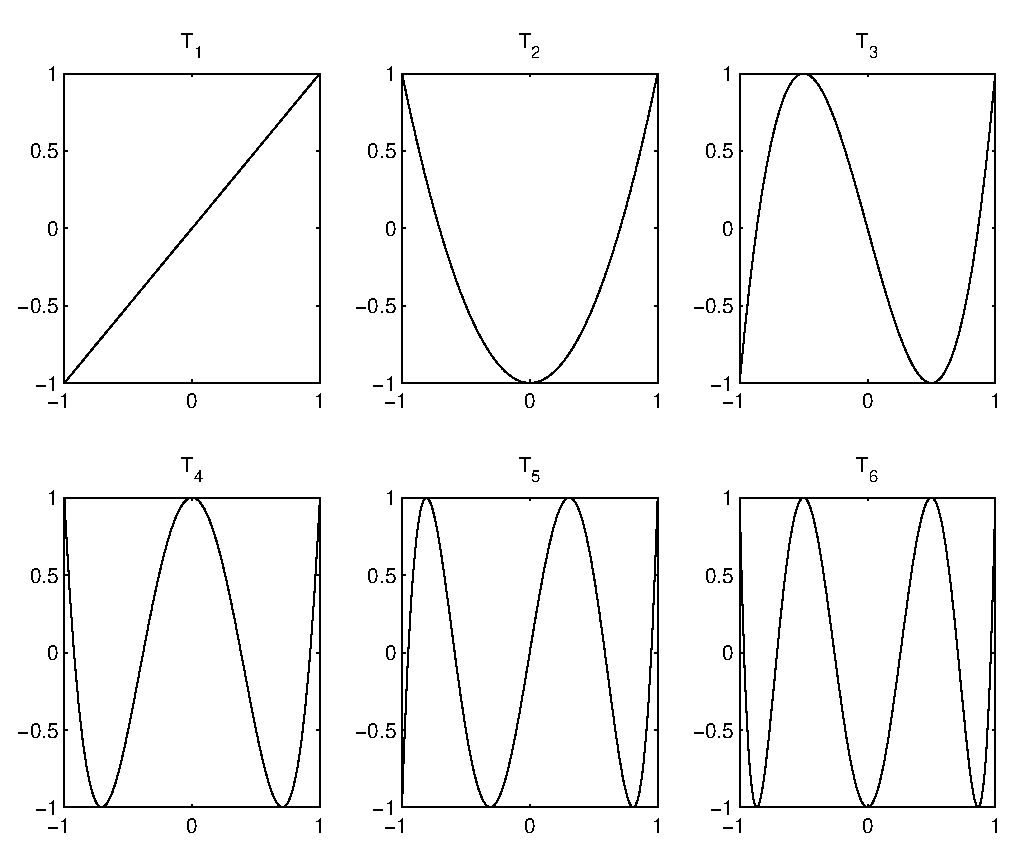
\includegraphics [scale = 0.6]{images/polynomes-chebyshev.eps}
    \end{center}
    \caption{Polynomials $ T_k $ for $ k = 1, \ldots, \, 6 $}
              \label{fig-polynomes-chebyshev}
\end{figure}
We consider a continuous function $ f: [-1,1] \rightarrow \RR $. We want to interpolate it in $N$ points $ \{x_k\}_{k = 0}^{N-1} $ by a polynomial $ P_{N-1} $ of degree $ N-1 $, where the $ x_k $ are defined by
\begin{equation*}
\forall k \in \{0, \ldots, \, N-1\}, \quad x_k \eqdef \cos \left((k + 1/2) \frac{\pi}{N} \right).
\end{equation*}
\begin{enumerate}
\item Show that $ T_N $ is indeed a polynomial, by determining a recurrence relation between $ T_k $ and $ T_{k-1} $. Show that the roots of $ T_N $ are $ x_k $, for $ k \in \{0, \ldots, \, N-1\} $.
\item Show that $ P_{N-1} $ can be put in the form
\begin{equation*}
P_{N-1} = \sum_{k = 0}^{N-1}{\alpha_k T_k}.
\end{equation*}
 
\item \index{Compression!JPEG} \index{JPEG} \index{Inversion formula} We consider two types of discrete cosine transforms (often denoted DCT-2 and DCT-3 in English, because there are d'others) of a sample $ \{f[k]\}_{k = 0}^{N-1} \in \RR^N $:
\begin{align*}
\Cc_2 (f) [j] & \eqdef \sum_{k = 0}^{N-1}{f[k] \cos \left((k + 1/2) \frac{j \pi}{N } \right)} \\
\Cc_3 (f) [j] & \eqdef \frac{1}{2} f[0] + \sum_{k = 1}^{N-1}{f[k] \cos \left((j + 1/2) \frac{k \pi}{N} \right)}.
\end{align*}
\index{Matlab@\Matlab{}} Show that the inverse of $ \Cc_2 $ is $ \frac{2}{N} \Cc_3 $. Implement in \Matlab{} these transforms using a DFT of size $ 4N $ (we can think of making the signal even, then inserting 0 at odd indices). For more information on the cosine transform, we can consult the article of \nompropre{Strang}{\upshape \cite{strang-dct}}. Note that it is the transform $ \Cc_2 $ which is used for the compression of JPEG images.
\item How to calculate the $ \{\alpha_k\}_{k = 0}^{N-1} $ from $ \{f[k] = f(x_k)\}_{k = 0}^{N-1} $? Conclude a fast polynomial interpolation algorithm at the points $ x_k $.
\end{enumerate} The figure \figref{fig-interpolation-chebyshev} shows a comparison between the Lagrange interpolation (equidistant points) and the Chebyshev interpolation on a seemingly innocuous function:
\begin{equation*}
f(x) \eqdef \frac{1}{\alpha^2 + x^2} \quad \text{for} \quad \alpha \in \RR^*_+.
\end{equation*}
For the figure, we have taken $ N = 11 $, and $ \alpha = 0.3 $. Try, experimentally, to determine the value $ \alpha_0 $ from which the Lagrange polynomial uniformly converges to $ f $ when $ n \rightarrow + \infty $. \begin{figure}[ht]
    \begin{center}
    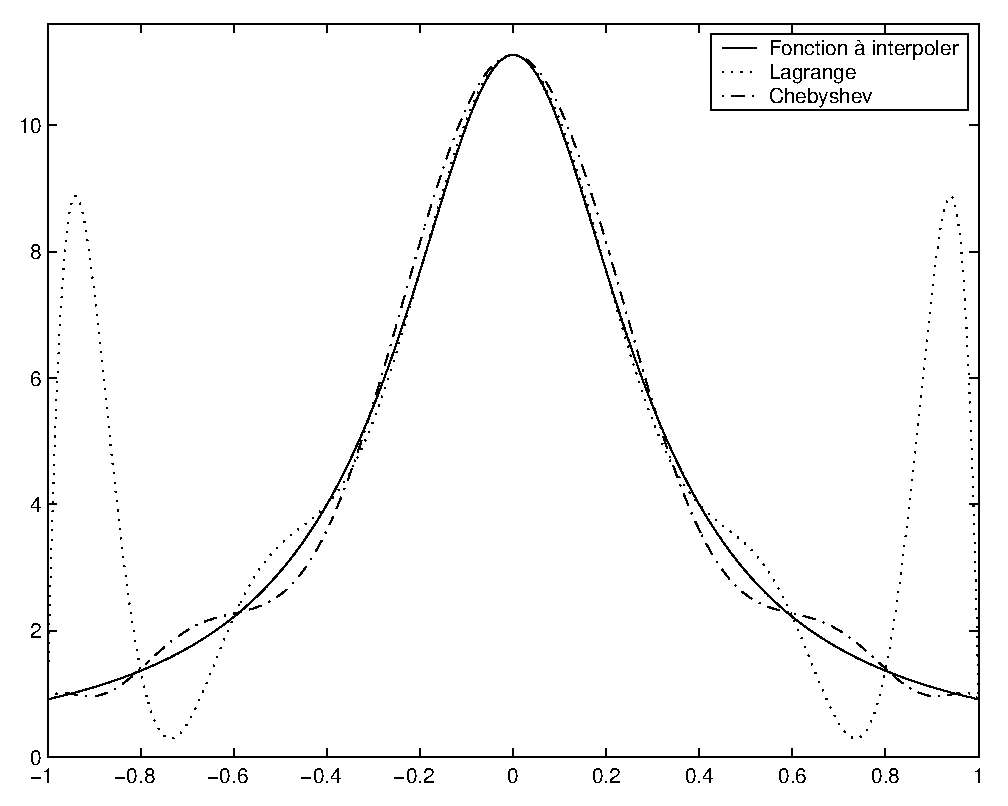
\includegraphics [scale = 0.4]{images/interpolation-chebyshev.eps}
    \end{center}
    \caption{Lagrange and Chebyshev interpolation}
              \label{fig-interpolation-chebyshev}
\end{figure}
\index{Method!spectral} Chebyshev interpolation is a simple case of spectral method. These methods use decompositions according to orthogonal polynomials to approximate the solutions of partial differential equations. This is an extension of Fourier series decompositions adapted to non-periodic functions. This is all very well described in \nompropre{Boyd}{\upshape \cite{boyd-spectral}}.
\end{exo}
 
 
\begin{exo}[Fractional derivation]
\label{exo-derivation-fractionionnaire}
 
\index{Fractional derivation} Let $ f: \RR \rightarrow \RR $ be a function of class $ \CC^\infty $ rapidly decreasing to infinity. Show that the Fourier transform (defined by the equation \eqref{eq-transforme-fourier-R}) of $ f^{(n)} $ is
\begin{equation*}
\Ff(f^{(n)}) (\xi) = (- \imath \xi)^{- n} \Ff(f) (\xi).
\end{equation*}
Explain how this property allows us to define a \textit{fractional derivation}, ie we can define a derivation for real values of $ n $. Implement a \Matlab{} routine which performs an approximate fractional derivative calculation using the FFT algorithm. The figure \figref{fig-derivation-fractionionnaire} shows the fractional derivative of a Gaussian obtained by this method, and this for different values of $ n $ between 0 and 2. \begin{figure}[ht]
    \begin{center}
    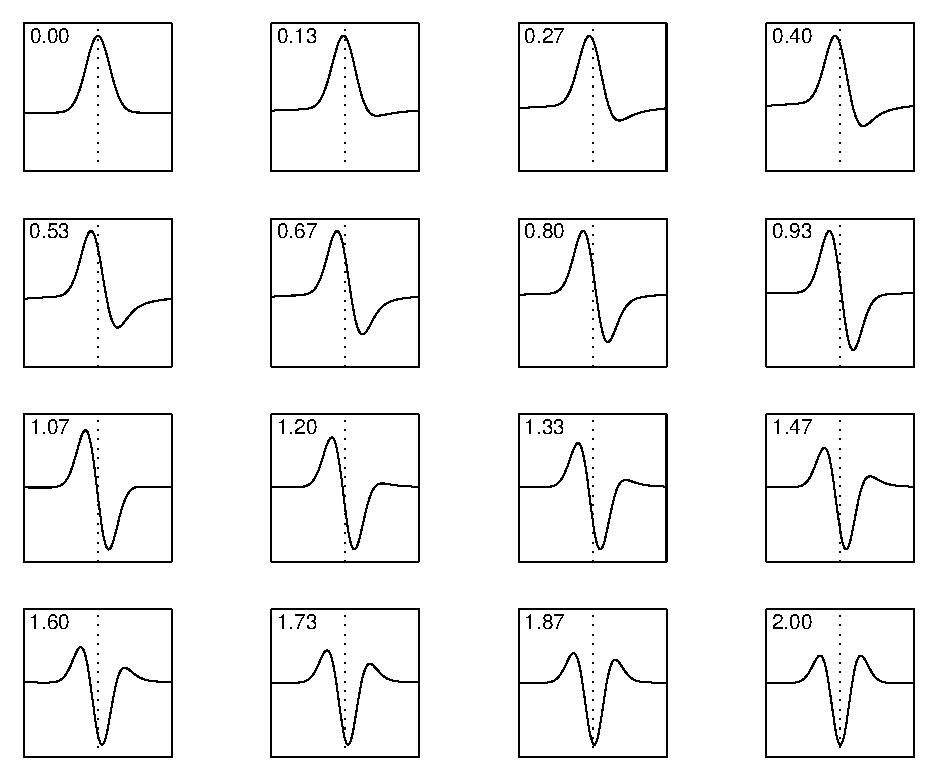
\includegraphics [scale = 0.5]{images/derivation-fractionnaire.eps}
    \end{center}
    \caption{Successive fractional derivatives of a Gaussian}
              \label{fig-derivation-fractionionnaire}
\end{figure}
\end{exo}
 
 
\begin{exo}[Intermediate Fourier transform]
\label{exo-transforme-partial-fourier}
 
\index{Fourier!intermediate!transform} \index{Normal!Endomorphism} \index{Unit!Endomorphism} \index{Unit!matrix} \index{Diagonalization} \index{Fourier!intermediate!Transform} We recall that we Note $ \Omega_N $ the Fourier matrix, which is defined by the equation \eqref{eq-defn-matrix-fourier}. It is a self-joined matrix, so like any normal endomorphism (i.e. which commutes with its adjunct), it diagonalizes to the orthonormal basis of $ \CC^N $ (which is false in $ \RR^N $). This means that there exists a unitary $ P $ matrix and a diagonal $ D $ matrix such that
\begin{equation*}
\Omega_N = PDP^{*}.
\end{equation*}
\begin{enumerate}
\item What are the entries of $ D $? Check this with \Matlab{}, by using the command \texttt{eig} which provides the eigenvalues as well as a decomposition according to the eigenvectors. It will be noticed that as the number of distinct eigenvalues is lower than $N$, the choice of the orthonormal basis of eigenvectors is totally arbitrary.
\item We define the matrix $ \Omega_N^{\alpha} $, for $ \alpha \in \RR $, by
\begin{equation*}
\Omega_N^{\alpha} \eqdef PD^{\alpha} P^{*},
\end{equation*}
where $ D^{\alpha} $ is \textit{one} power \ordin{\alpha}{th} of $ D $. We then define intermediate Fourier transforms:
\begin{equation*}
\forall f \in \CC^N, \quad \Ff^{\alpha} (f) \eqdef \Omega_N^{\alpha} f.
\end{equation*}
Show that we have
\begin{equation*}
\forall (\alpha, \beta) \in \RR^2, \quad \Ff^{\alpha} \circ \Ff^{\beta} = \Ff^{\alpha + \beta} \quad \text{and} \quad \Ff^1 = \Ff.
\end{equation*}
 
\item The figure \figref{fig-matrix-partial-tfd} shows the modulus of the matrix $ \Ff^{\alpha} $ for a parameter $ \alpha $ varying between $ 0.3 $ and $ 1 $. What do the two white diagonals that we can distinguish represent (we can use the calculation of the matrix $ \Omega_N^2 $)? 

\begin{figure}[ht]
    \begin{center}
    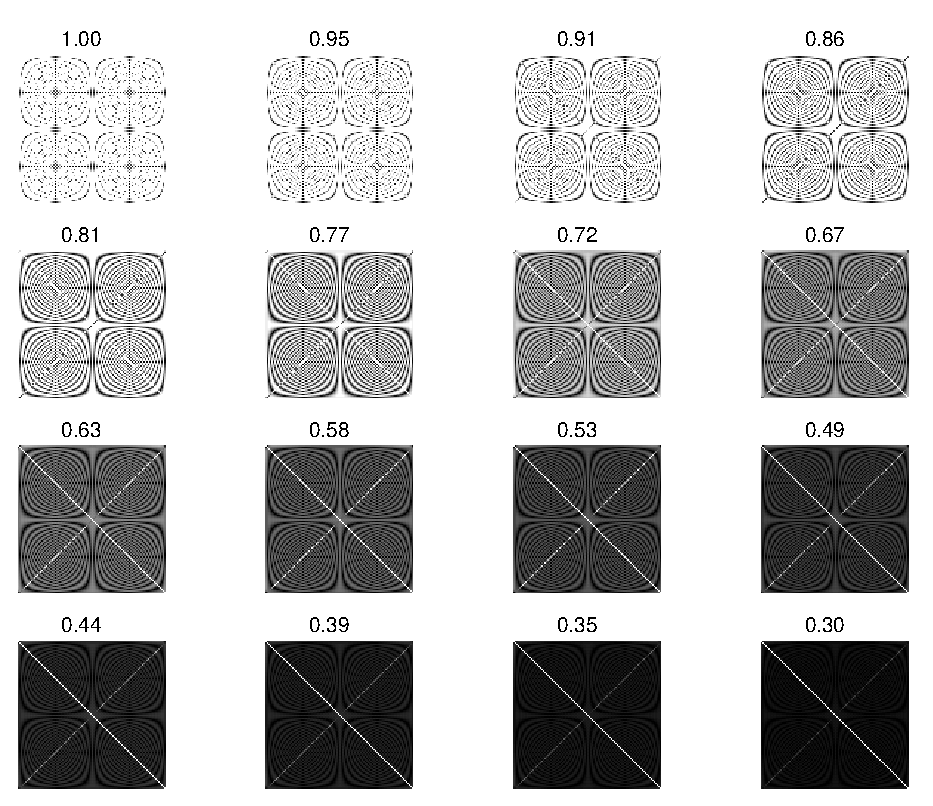
\includegraphics [scale = 0.5]{images/matrice-tfd-partielle.eps}
    \end{center}
    \caption{Modulus of different partial Fourier transform matrices}
              \label{fig-matrix-partial-tfd}
\end{figure}
 
\item Explain why we can construct an infinite number of intermediate transforms. By letting \Matlab{} decide on a factorization of $ \Omega_N $, implement the obtained transform, then test it with different values of $ \alpha $ and different signals.
\end{enumerate} Figure \figref{fig-transforme-partial-fourier} shows a panel of intermediate transforms for a Gaussian. The $ \alpha $ transformation parameter varies between $ 0 $ and $ 2 $. Of course, for $ \alpha = 2 $, we find the original signal (because the Gaussian is symmetrical). 

\begin{figure}[ht]
    \begin{center}
    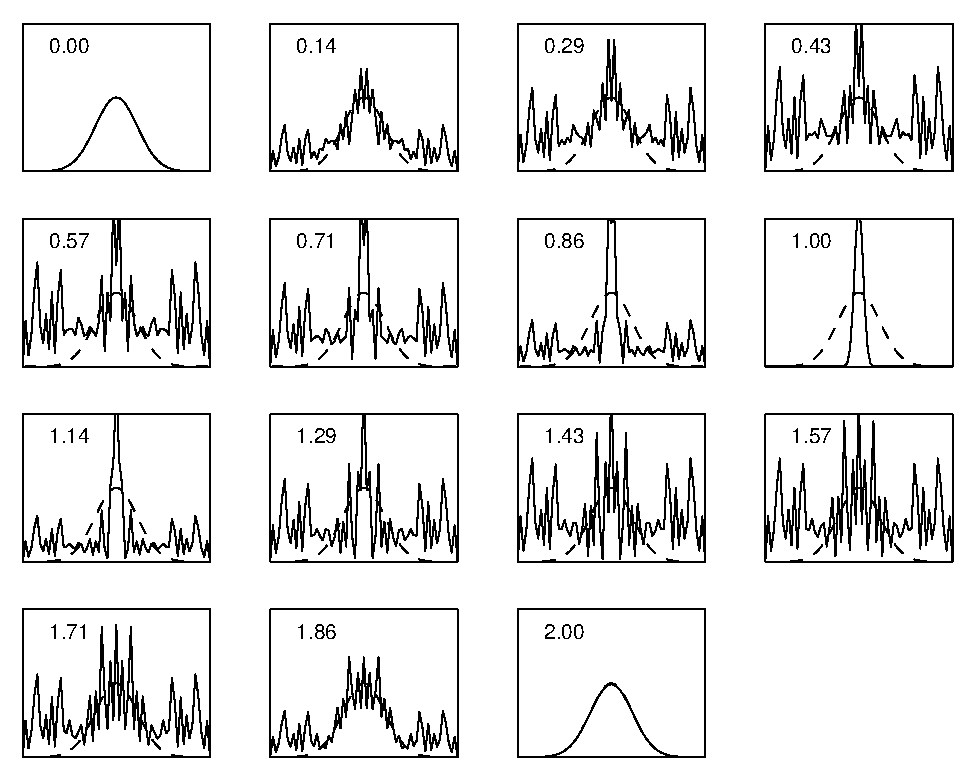
\includegraphics [scale = 0.5]{images/transformee-fourier-partielle.eps}
    \end{center}
    \caption{Successive partial Fourier transforms of a Gaussian}
              \label{fig-transforme-partial-fourier}
\end{figure}
\end{exo}
 
 
\begin{exo}[Diagonalization of the TFD]
\label{exo-diagonalization-tfd}
 
\index{Diagonalization} \index{Orthonormal basis} \index{Eigenvector} In the previous exercise, we used \Matlab{} to diagonalize the matrix of the TFD into orthonormal basis. The theoretical construction of an orthonormal basis is not simple, mainly because the eigenvalues have a multiplicity greater than 1, which leaves a potentially infinite choice of decompositions. The goal is therefore to build a canonical process to determine a basis for diagonalization. This exercise is inspired by the article by \nompropre{Dickinson}{\upshape \cite{dickinson-eigenvectors}}. We can also read the article of \nompropre{Candan}{\upshape \cite{candan-fractional}} which makes the relation between the matrix $ S $ and the discretization of a differential equation. \begin{enumerate}
\item \label{notation-50} \label{notation-51} We define a matrix $ S \in M_N (\RR) $ as follows:
\begin{equation*}
S \eqdef \begin{pmatrix} C_0 & 1 & 0 & \ldots & 1 \\1 & C_1 & 1 & \ldots & 0 \\0 & 1 & C_2 & \ldots & 0 \\\vdots & \vdots & \vdots & \ddots & \vdots \\1 & 0 & 0 & \ldots & C_{N-1} \end{pmatrix} \quad \text{where} \quad C_k \eqdef 2 \left(\cos \left(\frac{2k \pi}{N} \right) - 2 \right).
\end{equation*}
Explain why $ S $ diagonalizes in orthonormal basis.
\item \index{Circulating!Matrix} Show that $ S $ and $ \Omega_N $, the Fourier matrix, commute, that is, $ S \Omega_N = \Omega_N S $. We can decompose $ S $ into $ S = \Gamma + \Delta $, where $ \Gamma $ is a circulating matrix cleverly chosen so that $ \Omega_N \Gamma = \Delta \Omega_N $.
\item Show that if $ f $ and $ g $ are two diagonalizable endomorphisms of $ \CC^N $ which commute, then there exists a common basis of diagonalization.
\item \index{Unit!Endomorphism} \index{Unit!Matrix} We want to show that the eigenvalues of $ S $ are distinct. Let $ P $ be the unit endomorphism matrix of $ \CC^N $ which sends an element $ f $ of $ \CC^N $ to
\begin{align*}
\forall n \in \left\{1, \ldots, \, \lfloor (N-1) / 2 \rfloor \right\}, \quad P f[n] & \eqdef \frac{f[n] + f[-n]}{\sqrt{2}}, \\
\forall n \in \left\{\lceil (N + 1) / 2 \rceil, \ldots, \, N-1 \right\}, \quad P f[n] & \eqdef \frac{f[n ] - f[-n]}{\sqrt{2}}.
\end{align*}
and $ P f[0] = f[0] $. In the case where $N$ is even, we must also add $ P f[N / 2] = f[N / 2] $. Show that this operator is symmetric and orthogonal, and that it corresponds to the decomposition of $ f $ into its symmetric and antisymmetric parts. Then show that $ PSP^{-1} $ is a symmetric tridiagonal matrix.
\item \index{Method!of Givens-Householder} Show that the eigenvalues of a symmetric tri-diagonal matrix with non-zero diagonal elements are distinct. We can use the book of \nompropre{Ciarlet}{\upshape \cite{ciarlet}} which describes the Givens-Householder method to calculate the eigenvalues of a symmetric matrix. Conclude that the eigenvalues of $ S $ are quite distinct.
\item Deduce that we have thus built in a canonical way an orthonormal basis of eigenvectors of $ \Omega_N $.
\end{enumerate} In the figure \figref{fig-eigenvectors-tfd} we can see the modulus of the first eigenvectors of the DFT (i.e. those which have the least sign changes) constructed using the method just described. In the figure \figref{fig-matrix-eigenvectors-tfd} we can see the matrix of the moduli of the eigenvectors of the DFT (the large coefficients are black). \begin{figure}[ht]
    \begin{center}
    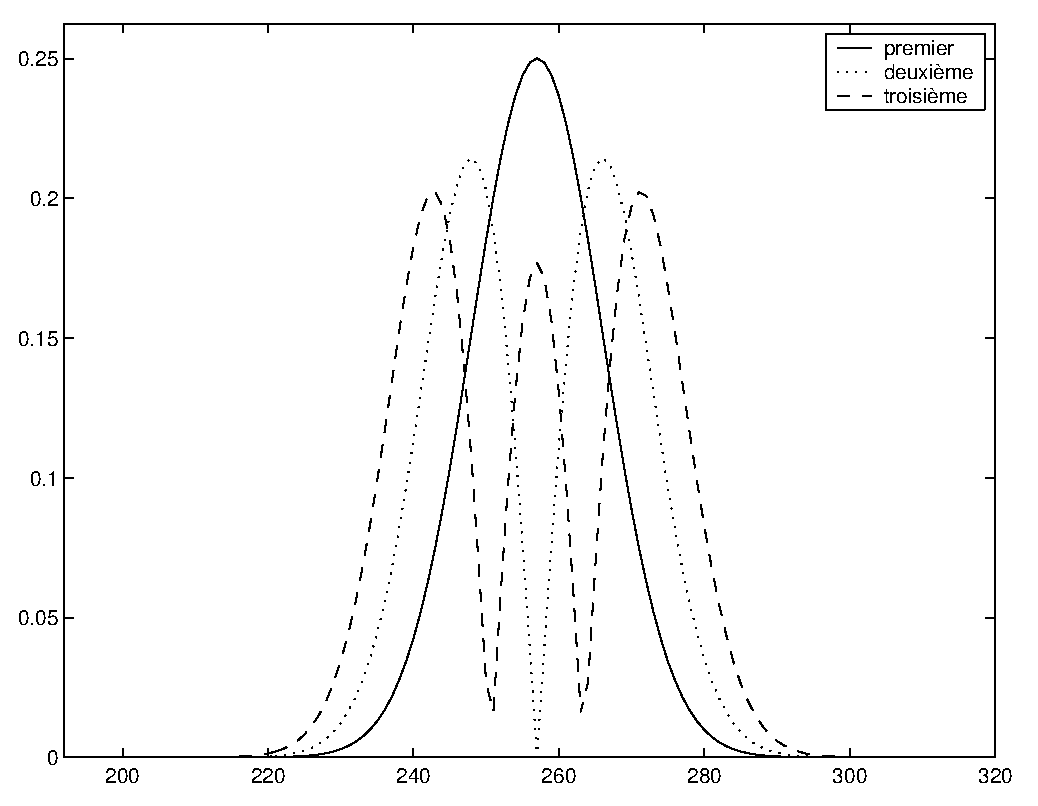
\includegraphics [scale = 0.4]{images/vecteurs-propres-tfd.eps}
    \end{center}
    \caption{Modules of some eigenvectors of $ \Omega_N $}
              \label{fig-eigenvectors-tfd}
\end{figure}
\begin{figure}[ht] 
    \begin{center}
    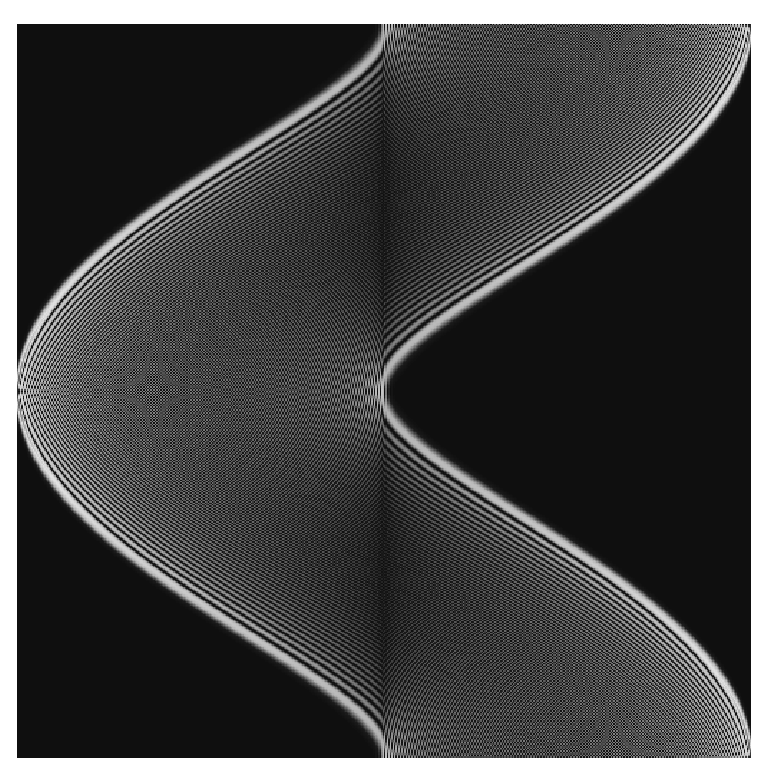
\includegraphics[scale=0.5]{images/matrice-vecteurs-propres-tfd.eps}
    \end{center}
    \caption{Matrix of moduli of orthogonal eigenvectors}
              \label{fig-matrix-eigenvectors-tfd}
\end{figure}
\end{exo}
 
 
\begin{exo}[Orthogonalization on a cyclic group]
\label{exo-orthogonalization-fourier}
 
This exercise studies in a particular case the notion of orthogonalization introduced in the exercise \oldref{exo-orthogonalization-abelian-group}. It is however independent. We consider the finite group $ G = \ZZ/n \ZZ $, as well as the vector space $ \CC [G] $ of functions from $ G $ in $ \CC $. For $ f \in \CC [G] $ and $ k \in G $, we define two actions of $ G $ on $ \CC [G] $ by setting
\begin{equation*}
k \top f: x \mapsto f(xk) \quad \quad \text{and} \quad \quad k \bot f: x \mapsto \omega^{- kx} f(x),
\end{equation*}
where we noted $ \omega_n \eqdef e^{\frac{2 \imath \pi}{n}} $. \begin{enumerate}
\item Show that the operations $ \top $ and $ \bot $ are related by
\begin{equation*}
\Ff(k \top f) = k \bot \Ff(f) \quad \quad \text{and} \quad \quad \Ff(k \bot f) = k \top \Ff(f).
\end{equation*}
 
\item We recall that $ f $ is said to be orthonormal under the action of $ \top $ if $ \{k \top f\}_{k \in G} $ is an orthonormal basis of $ \CC [G] $ . Using the previous question, explain how the orthonormal bases for $ \top $ and the orthonormal bases for $ \bot $ are related.
\item Show that $ f $ is orthonormal for $ \top $ if and only if $ \forall k \in G, \; | \wh{f}[k] | = $ 1.
\item Let $ f \in \CC [G] $ be such that $ \wh{f} $ does not vanish. We then define $ f_0 \in \CC [G] $ by
\begin{equation*}
\forall k \in G, \quad \wh{f_0}[k] = \frac{\wh{f}[k]}{| \wh{f}[k] |}.
\end{equation*}
Show that $ f_0 $ is orthonormal for $ \top $. Suggest a similar construction for $ \bot $.
\item \index{Correlation} We now assume that $ g $ is orthonormal for $ \top $. Let $ \varphi \in \CC [G] $ be any. We denote, for $ k \in G $, $ \Gg (\varphi) [k] \eqdef \dotp{\varphi}{k \top g} $ the decomposition coefficients of $ \varphi $ in the orthonormal basis $ \{k \top g\}_{k \in G} $. Show that $ \Gg (\varphi) = \frac{1}{n} f * \wt{g} \eqdef \frac{1}{n} \Corr (\varphi, \, g) $, where $ \wt{g}[k] \eqdef \ol{g [-k]} $, and $ \Corr $ is by definition the correlation of two vectors (see also the exercise \oldref{exo-correlation-2d} for the correlation of two images). Deduce a fast algorithm for calculating $ \Gg (\varphi) $ in $ O(n \log (n)) $ operations.
\end{enumerate} Figure \figref{fig-orthogonalisation-fourier} shows two examples of orthogonalization. The top function, which is closer to orthogonality than the bottom one (we see it on the moduli of Fourier coefficients which are far from $ 1 $), gives rise to a less oscillating function $ g $. Intuitively, to orthogonalize any function, we need the \guill{to oscillate}. \begin{figure}[ht]
    \begin{center}
    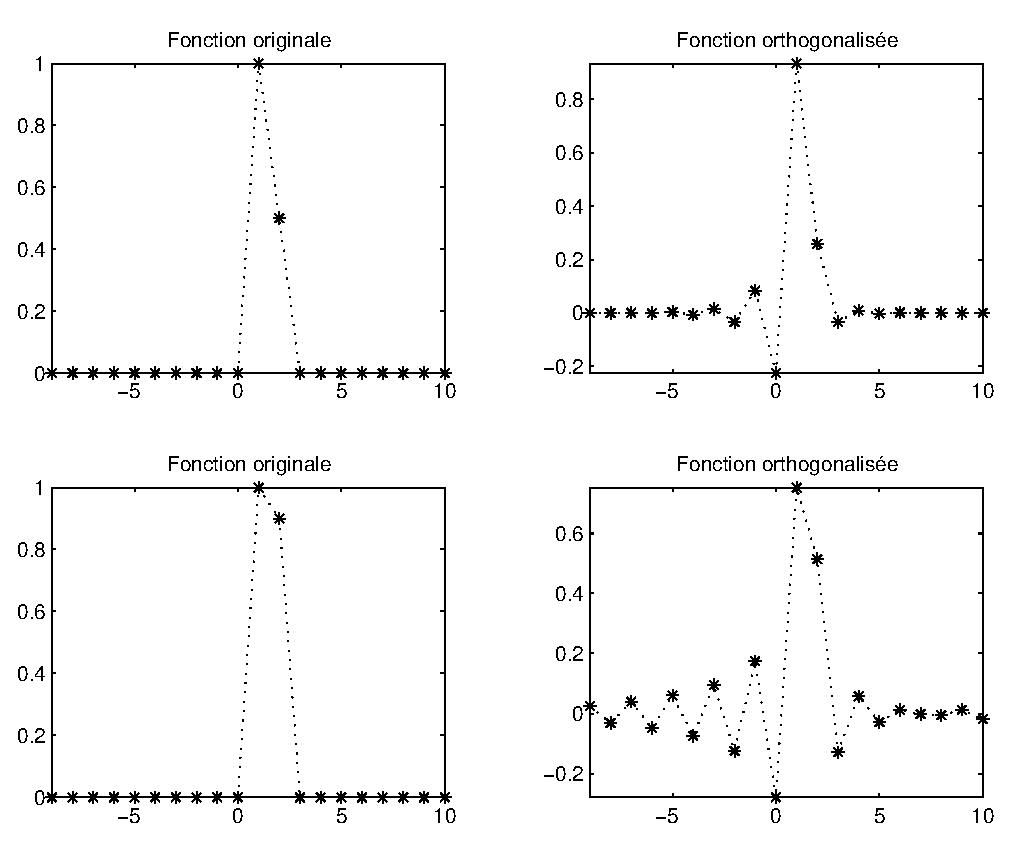
\includegraphics[scale=0.5]{images/orthogonalisation-fourier.eps}
    \end{center}
    \caption{Examples of orthogonalization}
              \label{fig-orthogonalisation-fourier}
\end{figure}
\end{exo}
 
 
\chapter{Applications of the discrete Fourier transform}
\label{chap-applications-tfd} 
 
 
 
We therefore saw, in the previous chapter, that we have an efficient algorithm, the FFT algorithm, to calculate the discrete Fourier transform. From then on, all applications using Fourier theory from near or far will be able to benefit from this algorithmic \guill{find}. But this phenomenon goes even further, since many other problems, however far removed from harmonic analysis, will be solved quickly thanks to the FFT algorithm. We will thus see that we can quickly calculate products of large integers, or even approach the solution of the Poisson equation, which may seem somewhat disconnected from the concerns we had until then!
 
% ------------------------------------------------- -----
% ------------------------------------------------- -----
% ------------------------------------------------- -----
% section - Link with the Fourier transform on $ \RR $                            
% ------------------------------------------------- -----
% ------------------------------------------------- -----
% ------------------------------------------------- -----
\section{Link with the Fourier transform on $ \RR $}
% \addcontentsline{toc}{section}{Link with the Fourier transform on $ \RR $}
\label{sect1-link-trans-fourier-R} 
 
This chapter is above all useful to better understand intuitively the discrete Fourier transform, thanks to many analogies with the continuous Fourier transform. It is not there to give the DFT a numerical nature, because it is above all necessary to conceive the discrete transform as an algebraic transformation, with an exact reconstruction formula (the inverse discrete Fourier transform). However, it is true that the FFT algorithm is often used to calculate Fourier coefficients in an approximate way, even if we will quickly see that the corresponding quadrature formula is not very precise.
% ------------------------------------------------- -----
% ------------------------------------------------- -----
% sub-section - Continuous Fourier transform                            
% ------------------------------------------------- -----
% ------------------------------------------------- -----
\subsection{Continuous Fourier transform}
\label{sect2-transforme-fourier-continue} 
 
 
\index{Fourier transform!on $ \RR $} We have just defined, in a way that we could qualify as abstract, the discrete Fourier transform. We can therefore naturally wonder if the latter has any relation to the usual Fourier transform on $ \RR $. The latter, for a function $ f \in L^1 (\RR) $ is defined by the equation
\begin{equation}
\label{eq-transforme-fourier-R}
\forall \xi \in \RR, \quad \wh{f} (\xi) \eqdef \int_{\minf}^{\pinf}{f(t) e^{- \imath \xi t} \d t}.
\end{equation}
This functional transformation has a very important meaning, particularly in the field of signal processing. If we consider that the function $ f $ represents a continuous signal which propagates in time, the Fourier transform makes it possible to pass from a temporal representation to a frequency representation. The quantity $ \wh{f} (\xi) $ intuitively represents how many variations there are at the frequency $ \xi $ in $ f $.
 
 
Moreover, we can extend by density the Fourier transform to functions $ f \in L^2 (\RR) $ of finite energy, i.e. such that $ \int_{\RR}{| f(x) |^2 \d x} <+ \infty $. Thus, the famous formula of \textit{Parseval}:
\begin{equation*}
\forall f \in L^2 (\RR), \quad \norm{\wh{f}}_{L^2} = 2 \pi \norm{f}_{L^2}
\end{equation*}
can be interpreted as a conservation of energy during the transition from the time domain to the frequency domain. For more details on the construction of the Fourier transform on $ \RR $, one can consult the book of \nompropre{Rudin} \cite{rudin}.
 
 
As for the Fourier transform on a finite group, we also have an inversion theorem, under somewhat restrictive assumptions.
 
\begin{prop}[Inversion formula]
\index{Inversion formula} When $ f \in L^2 $ and $ \wh{f} \in L^1 $, we have almost everywhere
\begin{equation}
\label{eq-formula-inversion-R}
f(x) = \frac{1}{2 \pi} \int_{\RR}{\wh{f} (\xi) e^{\imath x \xi} \d \xi}.
\end{equation}
\end{prop}
In fact, we could redo a character theory on the group $ (\RR, +) $ as it was done on finite abelian groups. Here is for example the determination of the characters of the real line:
 
\begin{prop}[Characters from $ \RR $]
\label{prop-characters-r}
\index{Character!of $ \RR $} \label{notation-52} We name the character of $ (\RR, +) $ the continuous morphisms of $ \RR $ in $ \Gamma \eqdef \enscond{z \in \CC}{| z | = 1} $. As usual, we denote by $ \wh{\RR} $ the group formed by the characters. For $ \gamma \in \RR $, either
\begin{equation*}
e_{\gamma}: \func{\RR}{\CC^*}{t}{e^{\imath \gamma t}}.
\end{equation*}
So we have $ \wh{\RR} = \{e_{\gamma} \}_{\gamma \in \RR} $ and the application $ \gamma \mapsto e_{\gamma} $ is an isomorphism between $ \RR $ and $ \wh{\RR} $.
\end{prop}
\begin{proof}
The $ e_{\gamma} $ are of course elements of $ \wh{\RR} $. Let $ \chi $ be a continuous morphism from $ \RR $ to $ \Gamma $. We will start by showing that $ \chi $ is a differentiable function. To do this, it suffices to integrate the homomorphism property in the neighborhood of $ 0 $:
\begin{equation*}
\int_0^h{\chi (s + t) \d t} = \chi (s) \int_0^h{\chi (t) \d t}.
\end{equation*}
As $ \chi (0) = 1 $, for $ h $ small enough, we have $ \int_0^h{\chi (t) \d t} \neq 0 $. We therefore have, for a certain $ h $,
\begin{equation*}
\chi (s) = \frac{\int_s^{h + s}{\chi (t) \d \d tt}}{\int_0^h{\chi (t) \d t}},
\end{equation*}
which clearly defines a continuously differentiable function. Note $ \lambda = \chi'(0) $. By factoring the rate of increase, we obtain
\begin{equation*}
\forall s \in \RR, \quad \chi'(s) = \lim_{t \rightarrow 0}{\frac{\chi (s + t) - \chi (t)}{h}} = \chi (s) \lim_{t \rightarrow 0}{\frac{\chi (t) - \chi (0)}{h}} = \lambda \chi (s).
\end{equation*}
Note that the only function $ f $ which checks $ f'= \lambda f $ and $ f(0) = 1 $ is $ s \mapsto e^{\lambda s} $. It only remains to show that $ \lambda \in \imath \RR $. Just use $ \chi (s) \ol{\chi (s)} = \chi (0) = $ 1. By differentiating this equality in 0, we find $ \lambda + \ol{\lambda} = 0 $.
\end{proof}
Thus, the inversion formula \eqref{eq-formula-inversion-R} is to be compared to the formula \eqref{prop-decomposition-serie-fourier}, on a finite group: we were in a way content to replace the sum finite by an integral. Similarly, we could analyze the decomposition of a function $ 2 \pi $ -periodic in Fourier series. This time, it would be to use the characters in the circle $ S^1 \eqdef \RR / 2 \pi \ZZ $, which are the functions
\begin{equation*}
\forall n \in \ZZ, \; \forall t \in \RR, \quad e_n (t) \eqdef e^{int}.
\end{equation*}
The decomposition formula of a periodic Fourier series function (under good assumptions, and specifying the direction of convergence) is once again an inversion formula, this time with a countable sum. For an introduction to Fourier series and integrals on a group, one can consult the book of \nompropre{Dym} and \nompropre{MacKean} \cite{dym}, chapter 4.
% ------------------------------------------------- -----
% ------------------------------------------------- -----
% sub-section - Approximate calculation of the Fourier transform on $ \RR $                            
% ------------------------------------------------- -----
% ------------------------------------------------- -----
\subsection{Approximate calculation of the Fourier transform on $ \RR $}
\label{sect2-calculus-trans-fourier-approach} 
 
 
\index{Calculus!approximate integrals} \index{Translation} Before embarking on approximate calculations of integrals, it is necessary to be aware that the discrete Fourier transform is not limited to such approximations. We can partly explain the \guill{intuitive} properties of the discrete Fourier transform by invoking approximations of the continuous Fourier transform. However, what makes the discrete Fourier transform work so well does not come from its ability to faithfully approach the continuous transform (it is even the opposite), but comes from the fact that it transposes the algebraic properties that we used for the real line (convolution, inversion, translation, ...) in the case of a finite and cyclic domain. It is therefore the algebraic properties of the DFT which make it a powerful tool in numerical analysis, and which make it possible to have simple and fast algorithms. In this paragraph, we will nevertheless explain the connections which connect, in terms of approximate calculations, the two transforms, discrete and continuous.
 
 
\index{Method!of rectangles} Of course, the correct method to approximate the continuous transform is to find the value of $ \wh{f} $ at certain points. Indeed, we know in practice the signal $ f $ only in the form of a sample $ \{f [n] \}_{n = 0}^{N-1} $, each value $ f [n ] $ being measured for a value of the parameter $ x $ equal to $ x_n \eqdef n \Delta $, for $ n = 0, \ldots, \, N-1 $. $ \Delta $ is the discretization step, that is to say the interval (of time if we consider a signal varying in time) between two measurements of the signal $ f $.
 
 
In the following, in order to simplify the explanations, it is assumed that $ N $ is an even integer. It is clear that given a sample of $ N $ values of the signal $ f $, it is futile to want to compute more than $ N $ independent values of the Fourier transform $ \wh{f} $. This intuitive remark will be confirmed by the following approximate calculation:
\begin{equation*}
\forall \xi \in \RR, \quad \wh{f} (\xi) \approx \Delta \sum_{n = 0}^{N-1}{f [n] e^{- \imath \xi x_n}}.
\end{equation*}
This approximation is obtained by using the method of the rectangles on the left to calculate in an approximate way the integral \eqref{eq-transforme-fourier-R}. For this approximation to have a meaning, it is of course necessary that outside the interval $ [0, \, N \Delta] $ the function $ f $ is otherwise zero, at least very rapidly decreasing.
 
 
We see then that by calculating the values of $ \wh{f} $ for values of the parameter $ \xi $ of the form $ \xi_k \eqdef \frac{2k \pi}{N \Delta} $ we obtain a writing particularly pleasant for the approximate calculation of $ \wh{f} (\xi_k) $:
\begin{equation}
\label{eq-approx-transforme-fourier-dft-1}
\wh{f} (\xi_k) \approx \Delta \sum_{n = 0}^{N-1}{f [n] e^{\frac{- 2 \imath \pi}{N} kn}} .
\end{equation}
As we mentioned before, it makes sense to only calculate $ N $ values of the Fourier transform, so we will apply the previous calculation to the points $ \xi_k $ for $ k $ variant in $ \{- N / 2 + 1, \ldots, \, N / 2 \} $. One might ask why we don't start at the index $ k = -N / 2 $, but we see that we get the same result for $ \xi_{- N / 2} $ and for $ \xi_{N / 2} $ (which conforms to our idea: no need to calculate more than $ N $ coefficients). By comparing the expression \eqref{eq-approx-transforme-fourier-dft-1} and the definition of the discrete Fourier transform \eqref{eq-defn-tfd}, we obtain
\begin{equation}
\label{eq-approx-transforme-fourier-dft}
\forall k \in \{0, \ldots, \, N-1 \}, \quad \wh{f} (\xi_k) \approx \Delta \wh{f}[k],
\end{equation}
where we have denoted $ \wh{f}[k] $ the \ordin{k}{ième} input of the discrete Fourier transform of the vector $ \{f [0], \ldots, \, f [N -1] \} \in \CC^N $ (as defined by the equation \eqref{eq-defn-tfd}).
 
 
However, there is a slight trick in the \eqref{eq-approx-transforme-fourier-dft} equation. Indeed, the index $ k $ varies in $ \{-N / 2 + 1, \ldots, \, N / 2 \} $, while the discrete transform vector $ \{\wh{f}[0 ], \ldots, \, \wh{f}[N-1] \} $ has its indices in $ \{0, \ldots, \, N-1 \} $. It is nevertheless easy to see that we did not make an error in writing the equality \eqref{eq-approx-transforme-fourier-dft}, since the discrete transform vector can be seen as a periodic function of period $ N $. We can therefore replace the negative frequencies $ \{- N / 2 + 1, \ldots, \, -1 \} $ by the frequencies $ \{N / 2 + 1, \ldots, \, N-1 \} $ : we get a vector whose indices vary between $ 0 $ and $ N-1 $.
 
 
Thus, the formula \eqref{eq-approx-transforme-fourier-dft} tells us that up to a factor $ \Delta $, the vector of the discrete Fourier transform $ \{\wh{f}[0], \ldots, \, \wh{f}[N-1] \} $ represents an approximation of the Fourier transform of the signal $ f $, but taken at very specific frequencies: the indices $ n $ between $ 0 $ and $ N / 2-1 $ correspond to the positive frequencies between $ 0 $ and $ f_c \eqdef \frac{\pi}{\Delta} $ (excluded), the indices $ n = N / 2 + 1, \ldots, \, N -1 $ correspond to the negative frequencies between $ -f_c $ (excluded) and $ 0 $ (excluded), while the index $ N / 2 $ corresponds to both the frequency $ f_c $ and $ -f_c $ (which is normal, since the transformed discrete signal is periodic with period $ N $). We must therefore pay attention to the following two points. \begin{rs}
\item The transformed vector $ \{\wh{f}[0], \ldots, \, \wh{f}[N-1] \} $ is considered as a periodic data of period $ N $ (it is the proper of the Fourier transform on an abelian group, in this case $ \ZZ/N \ZZ $). This is of course not the case with the function $ f: \RR \rightarrow \CC $ which has no reason to be periodic with period $ 2 f_c $.
\item Compared to the Fourier transform on $ \RR $ of the continuous signal $ f $, the frequencies are arranged in the order: negative frequencies, then positive frequencies.
\end{rs}
% ------------------------------------------------- -----
% ------------------------------------------------- -----
% sub-section - Addition of zeros                            
% ------------------------------------------------- -----
% ------------------------------------------------- -----
\subsection{Addition of zeros}
\label{sect2-addition-zeros} 
 
\index{Zero padding} There are two basic techniques for influencing how one can calculate, using the discrete transform, different values of the continuous transform. \begin{rs}
\item \index{Sampling} We can sample the signal with more or less precision. We have seen that the more precise the sampling is (that is to say the more points we take to represent the analyzed function), the wider the spectrum of the transform. Thus, if one wishes to cover a spectrum twice as large, it suffices to divide the interpolation interval by two. Of course, this also extends the time needed to do the math.
\item You can add zeros at the end of the vector. If we are satisfied with the spectrum on which we calculate the transform (more precisely the maximum and minimum frequencies that we can calculate), we may then want to calculate the transform with more precision, for example if we want to draw a curve to graphically represent the transform. In this case, the procedure is simple: it suffices to add zeros at the end of the vector, to add as many calculated intermediate frequencies.
\end{rs} By playing on these two parameters (interpolation precision and addition of zeros), we can calculate \guill{custom} discrete transforms, to have a certain fixed vector size (this can be used to create filters, see Section~\ref{sect1-filtering}), but also for the representation of the transform. The figure \figref{fig-calcul-approach-tf} shows the different results that can be obtained by adjusting both the number of sampling points and the addition of zeros. The functions represented are the modules of the DFT of the indicator function of $ [0.5, \, 1] $, sampled on $ [0, \, 1] $ at regular intervals. Each row uses the same number of sample points, but with more or less zeros added. \begin{figure}[ht]
    \begin{center}
    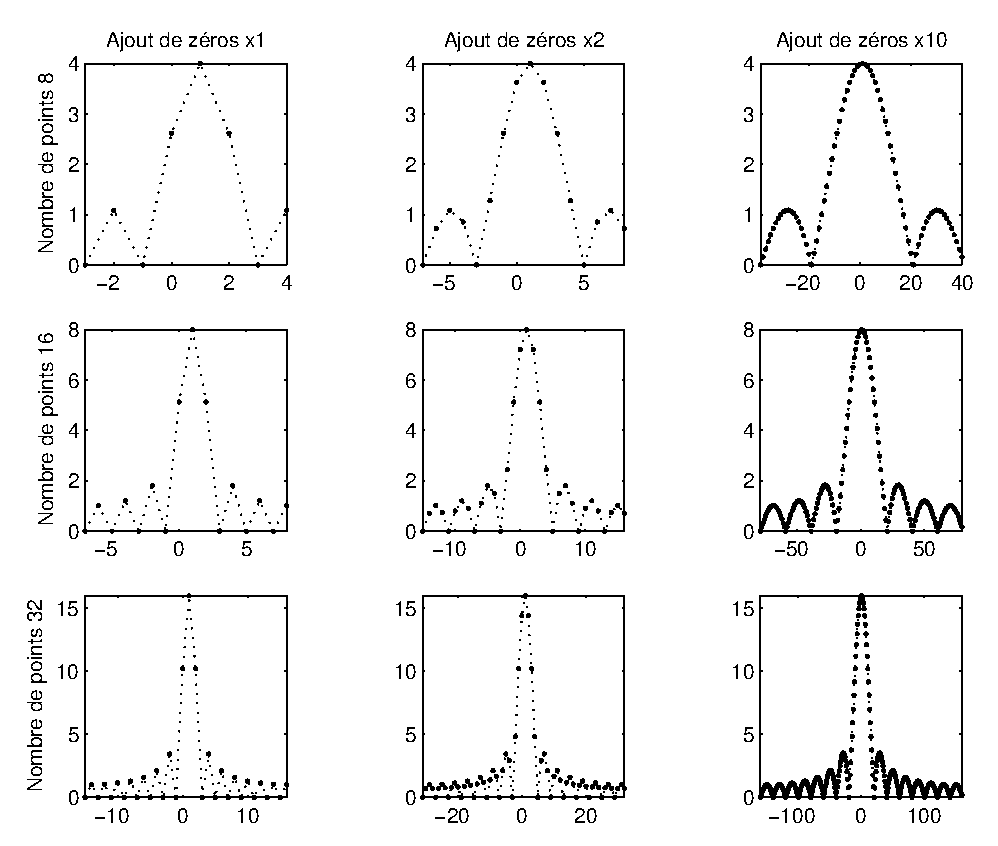
\includegraphics[scale=0.7]{images/calcul-approche-tf.eps}
    \end{center}
    \caption{Influence of sampling and adding zeros}
              \label{fig-calcul-approach-tf}
\end{figure}
The exercise \oldref{exo-creation-low-pass-filter} is instructive in this regard, since it reinvests all of this in order to create and test a low-pass filter.
% ------------------------------------------------- -----
% ------------------------------------------------- -----
% sub-section - Time / frequency duality                            
% ------------------------------------------------- -----
% ------------------------------------------------- -----
\subsection{Time / frequency duality}
\label{sect2-duality-time-frequency} 
 
 
\index{Uncertainty!principle} \index{Uncertainty} The approximate calculation we have just done allows us, via the use of the discrete Fourier transform, to calculate the value of the Fourier transform of a signal for certain frequencies only, precisely those of the form $ \frac{2 k \pi}{N \Delta} $ for $ k \in \{- N / 2 + 1, \ldots, \, N / 2 \} $. We therefore notice that the greater the precision with which the computation is carried out (that is to say the discretization step $ \Delta $ is small), the more the spectrum on which the transform is calculated is spread. This is not an isolated phenomenon, and results from a very strong duality between the starting function and its Fourier transform.
 
 
The following result clearly illustrates this duality between the temporal properties of a signal (that is to say the properties of a function $ f $) and its frequency properties (that is to say those of the transformed function $ \wh{f} $).
 
\begin{prop}
\label{prop-trans-fourier-support-compact}
\index{Support!compact} Let $ f $ be a function of $ L^2 (\RR) $. Then $ f $ and $ \wh{f} $ cannot simultaneously be compactly supported.
\end{prop}
The proof of this result is given in the exercise \oldref{exo-transforme-sup-comp}. This property has an immediate discrete analogue, which we can see by considering the discrete impulse $ \delta_0 $ (the vector which is worth 1 in 0, and which is zero everywhere else). Its discrete Fourier transform has a spectrum that covers the entire interval considered, since it is the exponential function $ t \mapsto e^{2 \imath \pi t} $ sampled at regular time intervals.
% ------------------------------------------------- -----
% ------------------------------------------------- -----
% ------------------------------------------------- -----
% section - Filtering                            
% ------------------------------------------------- -----
% ------------------------------------------------- -----
% ------------------------------------------------- -----
\section{Filtering}
% \addcontentsline{toc}{section}{Filtering}
\label{sect1-filtering} 
 
\index{Filter} The notion of filtering a sampled signal is easy to define, but is used in an intensive and varied manner. We will therefore not go around the question, however, it is interesting to link the technique of filtering with tools such as the FFT algorithm and linear convolution.
% ------------------------------------------------- -----
% ------------------------------------------------- -----
% sub-section - Linear filters                            
% ------------------------------------------------- -----
% ------------------------------------------------- -----
\subsection{Linear filters}
\label{sec2-linear-filters} 
 
 
\index{Filter!linear} \label{notation-53} Let us start by defining the filtering of a theoretical infinite signal, before looking at the practical computation on finite signals. The filtering of a signal $ f \in \CC^\ZZ $ consists in pairing (acyclically of course) this signal with another signal $ g \in \CC^\ZZ $ fixed in advance. We thus obtain a filter operator
\begin{equation*}
\Phi^g: \func{\CC^\ZZ}{\CC^\ZZ}{f}{f \star g}.
\end{equation*}
\index{Transfer!function} We say that $ g $ is the transfer function of the filter $ \Phi^g $.
 
 
\index{Impulse!response} One of the remarkable properties of linear filters is that they obtain the \textit{impulse response} (that is, how the system represented by the filter reacts to an impulse), which is calculated very simply:
\begin{equation*}
\Phi^g (\delta_0) = \delta_0 \star g = g,
\end{equation*}
where we noted $ \delta_0 $ the impulse in $ 0 $, that is to say the sequence which is worth $ 1 $ in $ 0 $, and which is zero everywhere else (we speak of \textit{discrete Dirac}). In other words, the filter transfer function is nothing more than the impulse response.
 
 
\index{Support} Once all these definitions have been exposed, we have to ask ourselves the question of the practical calculation of the filter. If we want to be able to calculate the convolution $ f \star g $ in a finite time, a natural assumption is to impose on the impulse response $ g $ to be finite (more precisely with finite support). It is a rather radical choice, but the interest is that it will allow us to apply a linear filter to finite signals in a very simple way. It will indeed suffice to use the acyclic convolution techniques already presented in Section~\ref{sect1-convolution-acyclic}. Let us briefly recall the procedure to follow. We suppose that the signal to be filtered is of the type: $ f = \{f [0], \ldots, \, f [N-1] \} $, and that the impulse response, it, is can be defined for negative indices, but is, in all cases, of finite size $ P $. We must: \begin{rs}
\item add enough zeros to the two vectors so that they reach the size of $ N + P-1 $.
\item move the negative index entries $ g $ to the end of the vector (this is customary for cyclic convolutions).
\item calculate the convolution \textit{cyclic} by FFT then inverse FFT.
\item extract the indices that interest us from the result and put them back in order (if we want to retrieve the entries with negative indices).
\end{rs}
 
 
One of the main characteristics of the convolution filters that we have just described is that they have a finite impulse response, in the sense that it becomes zero outside the support of $ g $. This is why we often name the convolution filters \textit{finite impulse response filters}, in English \textit{FIR} (for \textbf{F} inite \textbf{I} mpulse \textbf{R} esponse). We will see in Paragraph~\ref{sect2-application-trans-z-filters}, that we can easily build filters which do not have this property, but which can still be calculated in a finite time.
 
 
In most cases, the transfer function $ g $ has limited support in the neighborhood of $ 0 $ (that is, only inputs in the neighborhood of $ 0 $ are non-zero). A good example is the Gaussian filter, given by the equation
\begin{equation*}
\forall k \in \{- N / 2, \ldots, \, N / 2 \}, \quad g [k] = \frac{1}{M} \exp \left(- \frac{(2 k / N)^2}{2t} \right).
\end{equation*}
The parameter $ M $ is adjusted so that $ \norm{g}_1 \eqdef \sum_k{| g [k] |} = $ 1. The parameter $ t $ represents the variance of the Gaussian. The smaller $ t $, the more the Gaussian is \guill{picked}, so the more $ g $ tends towards the Dirac $ \delta_0 $ (and the filter $ \Phi^g $ tends towards the identity). On the contrary, the larger $ t $ becomes, the more the Gaussian is \guill{spread}, and the more the filter smooths the signal. We must pay attention to the fact that the indices of $ g $ have been taken from $ [- N / 2, \, N / 2] $, because we want to realize an acyclic filter. To perform a cyclic filter and / or calculate the filter by FFT, it is of course necessary to report the negative frequencies \textit{at the end} of the vector.
 
 
Figure \figref{fig-filter-smoothing} shows different Gaussian kernels (top). The left kernel has a variance $ t $ so low that it is equal to the Dirac. The bottom line shows the filtering of an irregular signal (shown on the left, since filtering by a Dirac has no effect). We see that the higher the variance, the more regular the filtered signal. This joins the classical theory of continuous convolution: when we filter by a kernel of class $ \Cc^\infty $ (for example a Gaussian), the function instantly becomes of class $ \Cc^\infty $, therefore extremely smooth!\begin{figure}[ht]
    \begin{center}
    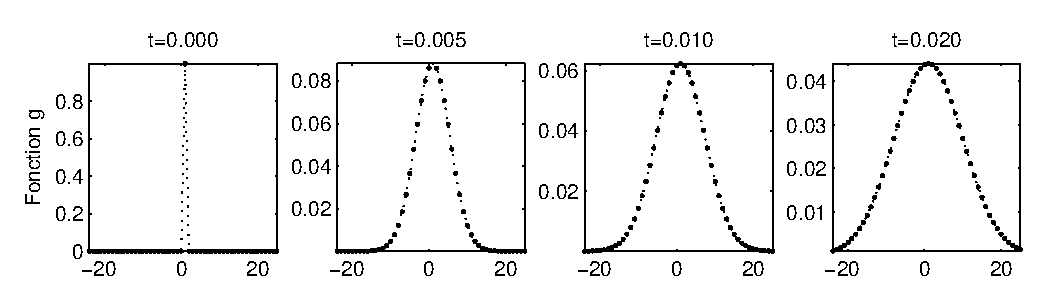
\includegraphics[scale=0.7]{images/filtre-lissage-1.eps}
    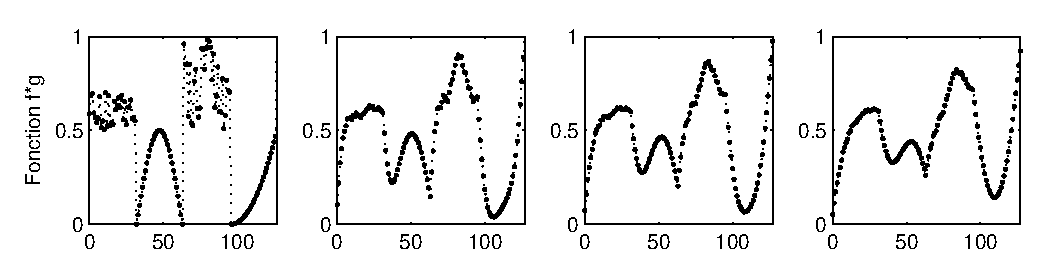
\includegraphics[scale=0.7]{images/filtre-lissage-2.eps}
    \end{center}
    \caption{Smoothing by a Gaussian}
              \label{fig-filter-smoothing}
\end{figure}
 
% ------------------------------------------------- -----
% ------------------------------------------------- -----
% sub-section - Types of responses and stability                            
% ------------------------------------------------- -----
% ------------------------------------------------- -----
\subsection{Response types and stability}
\label{sect2-responses-stability} 
 
 
We have therefore seen that the impulse response defines a filter. However, we can also characterize this filter by other types of responses, including: \begin{rs}
\item \index{Harmonic} \index{Frequency response} \textit{the frequency response}. It is simply the Fourier transform of the transfer function, i.e. $ \sum_{k \in \ZZ}{g [k] e^{\imath kx}} $, for $ x \in [- \pi, \, \pi] $. It is a $ 2 \pi $ -periodic function, since it is the Fourier series associated with the coefficients $ g [k] $. Since the impulse response $ g $ is finite, we can calculate it by discrete transform (FFT), by adding a lot of zeros at the end of $ g $ to have a very good precision (a quasi-continuous plot of the function, cf paragraph \ref{sect2-addition-zeros}). It represents how the filter operates in the frequency domain. Indeed, by using the convolution theorem \ref{prop-convol-tfd}, we see that the frequency response indicates by what quantity the filtering will multiply the amplitude of each harmonic (i.e. each component of the transformed vector) of the original signal.
\item \index{Step!Response} \textit{Step Response}. This is the vector obtained by filtering a step, that is to say the sequence which is zero for negative indices, and which is worth $ 1 $ for indices equal to or greater than $ 0 $. This response indicates how the filter will react to a discontinuity. For a normally constituted human mind, this is the answer that makes the most sense, since the human eye is above all trained to spot discontinuities. Thus, by observing the step response of a 2D filter, we will have indications on how the filter will transform the contours of the image (where there is a strong variation in intensity).
\end{rs} In a pragmatic way, the frequency response is calculated very simply by using the FFT algorithm (by taking care to add enough zeros to obtain sufficient precision, and by putting the negative frequencies back in their place) . For the step response, there are at least two ways to proceed. \begin{rs}
\item \index{Echelon} We can give a step at the input of the filter. For linear filtering, it suffices to give as input a constant vector equal to $ 1 $, the algorithm being supposed to add enough zeros to avoid circular convolution.
\item If we know the impulse response $ y_0 $ and we want to calculate the step response $ y_1 $, it suffices to notice that the step function is the discrete primitive (that is to say the partial sum), and therefore using the linearity of the filter, it will be the same for both responses. We thus obtain the simple formula
\begin{equation*}
\forall n \geq 0, \quad y_1 [n] = \sum_{k = \minf}^{n}{y_0 [k]}.
\end{equation*}
\end{rs} 
Figure \figref{fig-diff-types-responses} shows the three different response types for 3 different transfer functions. The first line represents a Gaussian, and we can see that the impulse response is also a Gaussian (which is logical, since the transform of a Gaussian is Gaussian, see the lemma \ref{lem-tf-gaussienne}). The other two lines show filters with a slower decay, and there are some oscillations in the frequency response. Note that filters are not causal, i.e. transfer functions are defined for negative indices. 

\begin{figure}[ht]
    \begin{center}
    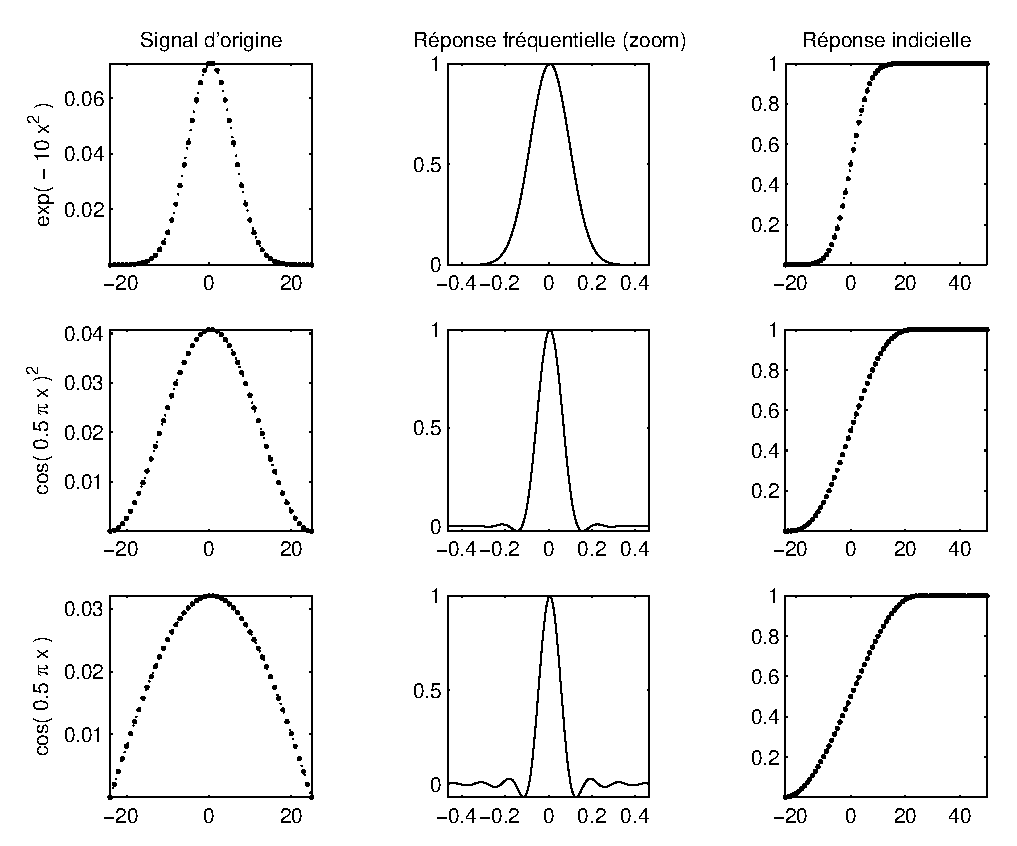
\includegraphics[scale=0.7]{images/diff-types-reponses.eps}
    \end{center}
    \caption{Frequency and index responses}
              \label{fig-diff-types-responses}
\end{figure}
 
 
 
 
 
\begin{rem}{(\upshape \textbf{Time and frequency domain}).} 
\index{Duality!time / frequency} \index{Support!compact} Depending on the answer that interests us, we can see a filter as operating in the time domain (even if the signal is not sampled in time but for example in space) or in the frequency domain. In certain applications, it is natural to create the filter according to the temporal properties which one wants to give to the filter (for example to smooth images in a privileged direction). In other applications, we will be interested in the frequency behavior of the filter (how the filter will remove high frequencies, for a low pass filter at the output of a microphone). The remarks on the time / frequency duality made in Paragraph~\ref{sect2-duality-time-frequency} explain that we cannot have it both ways. For example, if one wishes to create a very precise \textit{bandpass} filter (that is to say with the most compact support possible), it will necessarily be of little use in the time domain, because it will have a very wide impulse response.
\end{rem}
 
 
 
\label{notation-54} Before moving on to the study of two-dimensional filters, let us briefly present an important notion which will be taken up later (during the study of the transform in Z, in Paragraph~\ref{sect1-trans-Z}). This is the notion of \textit{stability} of a filter, which is defined in a very intuitive way.
 
\begin{defn}[Stability]
\index{Stability} A filter $ \Phi^g $ is said to be stable if for any bounded signal $ f \in \CC^\ZZ $, the output $ \Phi^g (\Phi) $ is also bounded.
\end{defn}
A simple calculation shows that
\begin{equation*}
\forall n \in \ZZ, \quad | \Phi^g (f) [n] | \leq \sup_{n \in \ZZ} (| f [n] |) \sum_{k = \minf}^{\pinf}{| g [k] |}.
\end{equation*}
Consequently, for a filter to be stable, it suffices that $ g \in \ell^1 (\ZZ) $, where we have noted $ \ell^1 (\ZZ) $ the space of sequences absolutely summable. We can verify that this condition is also necessary, by taking a sequence $ f $ such that $ f [k] g [-k] = | g [k] | $ (for $ k $ such as $ g [k] \neq $ 0). We then have, if $ g \notin \ell^1 (\ZZ) $,
\begin{equation*}
\Phi^g (f) [0] = \sum_{k = \minf}^{\pinf}{f [k] g [-k]} = \sum_{k = \minf}^{\pinf}{| g [k] |} = + \infty.
\end{equation*}
If $ g \in \ell^1 (\ZZ) $, the filter operator $ \Phi^g $ is a continuous endomorphism of the space of bounded sequences, and its norm is exactly $ \norm{g}_{\ell^1} $.
 
 
The linear filters with finite impulse response which have been considered up to now are therefore always stable. We will see in Paragraph~\ref{sect2-application-trans-z-filters}, that it is possible to build filters which do not have this nice property.
% ------------------------------------------------- -----
% ------------------------------------------------- -----
% sub-section - 2D filtering and image analysis                            
% ------------------------------------------------- -----
% ------------------------------------------------- -----
\subsection{2D filtering and image analysis}
\label{sect2-filtering-2d} 
 
 
\index{Filter!2D} \index{Image smoothing} \index{Image} We can of course consider two-dimensional convolution as it is explained in paragraph \ref{sect2-convolution-2d}. This gives rise to a filter $ \Phi^g $, which acts on two-dimensional signals $ f: \{0, \ldots, \, N-1 \} \times \{0, \ldots, \, N-1 \} \rightarrow \RR $. These signals can be represented as images, since in each \textit{pixel} $ (i, \, j) $ of the image, we have a light intensity $ f [i, \, j] $. More precisely, we most often restrict the end set to a finite set, for example $ \{0, \ldots, \, 255 \} $. These $ 256 $ values represent the famous \textit{levels of gray} which will be displayed on the screen.
 
 
To \guill{smooth} an image, we will once again consider transfer functions $ g $ tightened around $ 0 $, for example a Gaussian:
\begin{equation*}
\forall (k, \, l) \in \{- N / 2, \ldots, \, N / 2 \}^2, \quad g [k, \, l] = \frac{1}{M} \exp \left(- \frac{(2 k / N)^2 + (2 l / N)^2}{2t} \right).
\end{equation*}
The parameter $ M $ is as in the 1D case chosen such that $ \norm{g}_1 = 1 $, and $ t $ is adjusted according to the power of the desired smoothing. Figure \figref{fig-Gaussian-filter-2} shows different Gaussian kernels (top row) as well as an image smoothed by these same Gaussian kernels (bottom row). \begin{figure}[ht]
    \begin{center}
    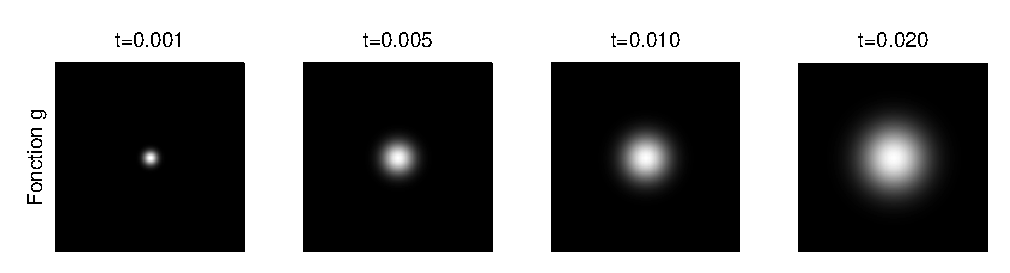
\includegraphics[scale=0.7]{images/filtre-gaussien-1.eps}
    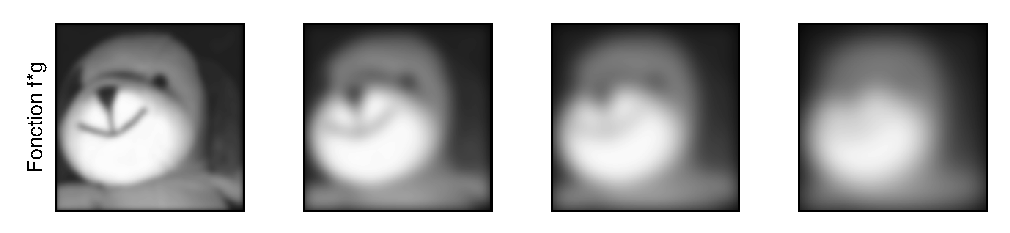
\includegraphics[scale=0.7]{images/filtre-gaussien-2.eps}
    \end{center}
    \caption{Smoothing of an image by a 2D Gaussian}
              \label{fig-Gaussian-filter-2}
\end{figure}
 
 
 
A very common application of image filtering is to soften the noise present in a degraded natural image. This is shown in the figure \figref{fig-filter-2d}, where we can see \textit{Maurice} whose image, of poor quality, has been improved by a Gaussian filter. 

\begin{figure}[ht]
    \begin{center}
    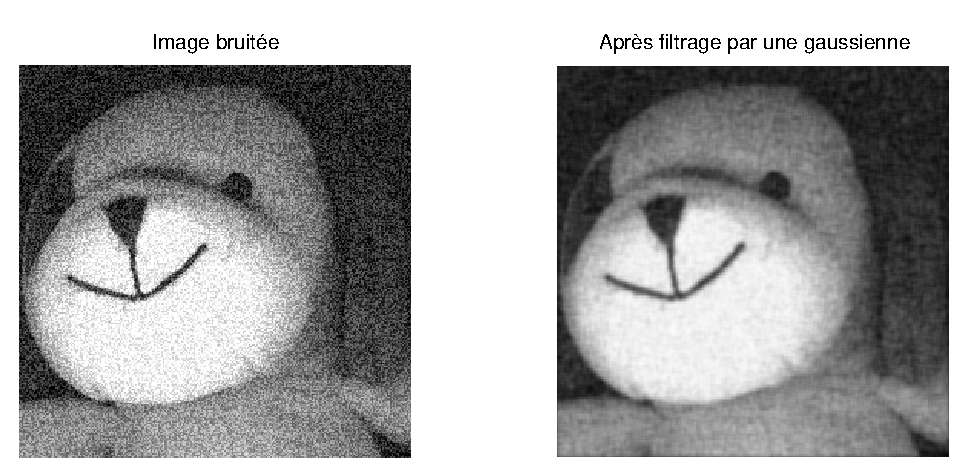
\includegraphics[scale=0.6]{images/filtre-2d.eps}
    \end{center}
    \caption{Image filtering example}
              \label{fig-filter-2d}
\end{figure}

The exercise \oldref{exo-correlation-2d} proposes to go further in image analysis, by applying the correlation calculation to the search for sub-images in a larger image.
% ------------------------------------------------- -----
% ------------------------------------------------- -----
% ------------------------------------------------- -----
% section - Geometric aspects of filtering                            
% ------------------------------------------------- -----
% ------------------------------------------------- -----
% ------------------------------------------------- -----
\section{Geometric aspects of filtering}
% \addcontentsline{toc}{section}{Geometric aspects of filtering}
\label{sect1-aspect-geometriques} 
 
In this section, we will approach the problem of filtering a signal from an original and simple angle, that of plane geometry. Rather than considering the signal studied as a series of values spaced in time, we will use it to describe a polygon drawn in the complex plane. We will then focus on the action of a filter on the shape of this polygon. More precisely, we will see how the successive iterates of the filtered polygon behave.
% ------------------------------------------------- -----
% ------------------------------------------------- -----
% sub-section - Polygon filtering                            
% ------------------------------------------------- -----
% ------------------------------------------------- -----
\subsection{Polygon filtering}
\label{sect2-filtering-polygons} 
 
 
\index{Polygon} \index{Filter!of polygons} In the rest of this talk, we will consider a polygon with $ N $ vertices, $ \Pi $, which we will see as a vector $ \Pi \in \CC^N $. Thus, $ \Pi [0] $ will represent the first vertex of the polygon, $ \Pi [1] $ the second, and so on. Equivalently, we can also consider a polygon as a function $ \Pi: \ZZ/N \ZZ \rightarrow \CC $. This description is very convenient, since it adapts well to the concept of closed polygon. Indeed, we consider that the vertex $ \Pi [i] $ is linked to the vertex $ \Pi [i + 1] $, and we naturally want to link the vertex $ \Pi [N-1] $ to the vertex $ \Pi [0] $. This amounts to considering a $ N $ -periodic signal.
 
 
\index{Iteration} We are interested in the action of a circular filter $ \Phi^g $ on a polygon $ \Pi $. We will therefore consider the iterated polygons $ \Pi^{(k)} $, for $ k \geq 0 $, which are defined as follows:
\begin{equation}
\label{eq-filtering-polygons}
\left\{\begin{array}{ll} \Pi^{(0)} = \Pi & \\\Pi^{(k)} = g * \Pi^{(k-1)} & \forall k> 0 \end{array} \right. ,
\end{equation}
where $ g $ is the filter transfer function. The natural question is to know if $ \Pi^{(k)} $ will tend towards a certain limit polygon, $ \Pi^{(\infty)} $, if the iterated polygons will remain bounded, or if on the contrary they will \guill{explode}. To carry out this study, it suffices to calculate the Fourier transform of the iteration relation \eqref{eq-filtering-polygons}, and we see that
\begin{equation*}
\forall k \geq 0, \quad \wh{\Pi^{(k)}} = (\wh{g})^n \cdot \wh{\Pi}.
\end{equation*}
The study of the convergence of $ \Pi^{(k)} $ is therefore very simple in the Fourier domain. Moreover, thanks to the inversion formula of the transform, a convergence in the Fourier domain is equivalent to a convergence of the polygon. Here are the different cases that can arise. \begin{rs}
\item If $ \exists i \in \{0, \ldots, \, N-1 \} $ such that $ | \wh{g}[i] | > $ 1: then the iterated polygons will explode. This corresponds to cases (a) and (b) in figure \figref{fig-filter-polygons-1}.
\item If for all $ i $, we have either $ | \wh{g}[i] | <1 $ or $ \wh{g}[i] = 1 $, then the iterated polygons will converge to a polygon $ \Pi^{(\infty)} $ which is defined by
\begin{equation*}
\forall i = 0, \ldots, \, N-1, \quad \wh{\Pi^{(\infty)}}[i] = \left\{\begin{array}{lll} 0 & \text{si} & | \wh{g}[i] | <1 \\\wh{\Pi}[i] & \text{si} & \wh{g}[i] = 1 \end{array} \right. .
\end{equation*}
This corresponds to case (c) of figure \figref{fig-filter-polygons-1}.
\item If $ \forall i \in \{0, \ldots, \, N-1 \}, \; | \wh{g}[i] | \leq 1 $, but there is a $ i $ such that $ | \wh{g}[i] | = 1 $ and $ \wh{g}[i] \neq 1 $, then the iterated polygons will not converge, but they will remain bounded. This corresponds to case (d) of figure \figref{fig-filter-polygons-1}. We can notice that if $ \wh{g}[i] $ is a root of unity, then the motion is periodic (even if the phenomenon is difficult to study numerically because of the rounding errors).
\end{rs} 

\begin{figure}[ht] 
    \begin{center}
    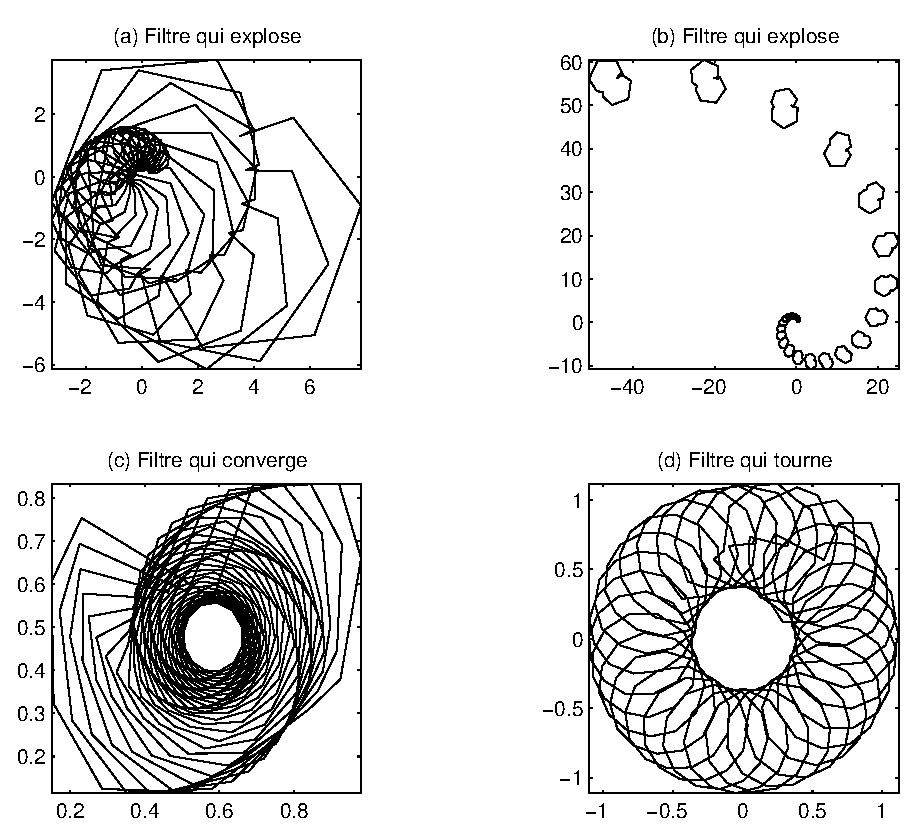
\includegraphics[scale=0.6]{images/filtre-polygones-1.eps}
    \end{center}
    \caption{Different cases of polygon filtering}
              \label{fig-filter-polygons-1}
\end{figure}

Two typical examples of polygon filtering can be given. They are shown in figure \figref{fig-filter-polygons-2}.
 
\begin{exmp}
\index{Center!of gravity} The first corresponds to the filter
\begin{equation*}
g = \{1/2, \, 1/2, \, 0, \ldots, \, 0 \}.
\end{equation*}
This consists of replacing the polygon $ \Pi $ by the polygon $ \Pi^{(1)} $ such that
\begin{equation*}
\Pi^{(1)}[i] = \frac{1}{2} \left(\Pi [i] + \Pi [i + 1] \right).
\end{equation*}
In a way, this amounts to joining the consecutive midpoints on each side of the polygon. Intuitively (and on the drawing of figure \figref{fig-filter-polygons-1}, on the left), one has the impression that the iterated polygons converge towards the center of the polygon. Let's confirm this by calculation:
\begin{equation*}
\wh{g}[k] = \frac{1}{2} \left(1 + e^{- \frac{2 \imath \pi}{N} k} \right) = \cos \left(\frac{k \pi}{N} \right) e^{- \frac{\imath \pi}{N} k}.
\end{equation*}
As we have $ \wh{g}[0] = 1 $ and for $ k \geq 1, \; | \wh{g}[k] | <1 $, we therefore conclude that the iterated polygons will converge to the point $ \wh{\Pi}[0] $, which corresponds to the center of gravity of the polygon.
\end{exmp}
 
 
\begin{exmp}
For the second example, this is a filter which acts in the Fourier domain as follows:
\begin{equation*}
\wh{g} = \{0.8, \, 1, \, 0.8, \ldots, \, 0.8 \}.
\end{equation*}
The iterated polygons will therefore converge to a polygon $ \Pi^{(\infty)} $ such that
\begin{equation*}
\wh{\Pi^{(\infty)}} = \{0, \, \wh{\Pi}[1], \, 0, \ldots, \, 0 \}.
\end{equation*}
We check that this corresponds to a regular polygon inscribed in a circle of radius $ | \wh{\Pi}[1] | $, as we can see in the figure \figref{fig-filter-polygons-2} (right).
\end{exmp}

\begin{figure}[ht] 
    \begin{center}
    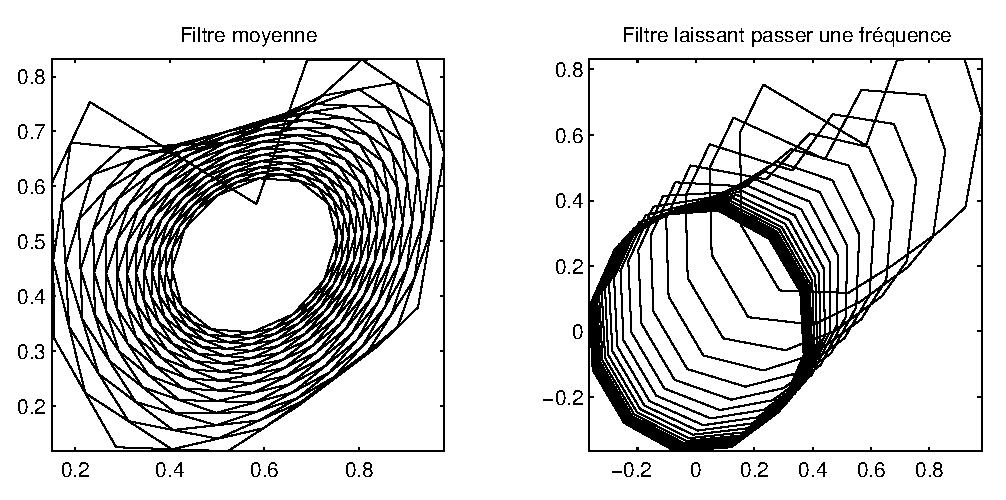
\includegraphics[scale=0.6]{images/filtre-polygones-2.eps}
    \end{center}
    \caption{Average filtering and frequency pass filtering}
              \label{fig-filter-polygons-2}
\end{figure}
 
% ------------------------------------------------- -----
% ------------------------------------------------- -----
% sub-section - Polygonal inequalities                            
% ------------------------------------------------- -----
% ------------------------------------------------- -----
\subsection{Polygonal inequalities}
 
 
\index{Inequality!polygonales} This paragraph is taken from the book by \nompropre{Terras} \cite{terras}. I wanted to insert it into a more general study of geometrical Fourier analysis, which is the subject of this paragraph. The idea is to use the Fourier transform in order to demonstrate inequalities of Euclidean nature on the polygons. The main tool will be the Plancherel equality \ref{prop-formula-floorel-tfd}, which will make it possible to demonstrate the inequalities by passing through the Fourier domain.
 
 
As in the previous paragraph, we consider a polygon $ \Pi $ with $ N $ sides, which can be seen as a function $ \Pi: \ZZ/N \ZZ \rightarrow \CC $. We will define several quantities related to this polygon. First, the sum of the squares of the lengths of the sides:
\begin{equation*}
S (\Pi) \eqdef \sum_{i = 0}^{N-1}{| \Pi [i + 1] - \Pi [i] |^2}.
\end{equation*}
\index{Distance} Then, the sum of the squares of the distances to the center of gravity of the polygon:
\begin{equation*}
T (\Pi) \eqdef \sum_{i = 0}^{N-1}{| \Pi [i] - \wh{\Pi}[0] |^2}.
\end{equation*}
Finally, the oriented area of the polygon:
\begin{equation*}
A (\Pi) \eqdef \frac{1}{2} \sum_{i = 0}^{N-1}{\imagp \left(\ol{\Pi [i]} \Pi [i + 1] \right)}.
\end{equation*}
 
 
\begin{prop}
We have the following inequalities: \begin{itemize}
\item [{\upshape (i)}] $ A (\Pi) \leq \frac{1}{2} T (\Pi) $
\item [{\upshape (ii)}] $ 4 \sin^2 \left(\frac{\pi}{N} \right) T (\Pi) \leq S (\Pi) $.
\end{itemize}
\end{prop}
\begin{proof}
\index{Offset operator} \textbf{Inequality (i)}: We introduce the offset operator $ T $ defined by the relation $ T \Pi [k] = \Pi [k + 1] $, which lets write
\begin{equation*}
A (\Pi) = \frac{1}{2} \imagp \left(\sum_{k = 0}^{N-1}{\Pi [i] \ol{T \Pi [i]}} \right).
\end{equation*}
Then just use Plancherel's formula to calculate $ A (\Pi) $ in the Fourier domain:
\begin{equation*}
A (\Pi) = \frac{1}{2} \imagp \left(\sum_{k = 0}^{N-1}{\wh{\Pi}[k] \ol{\Ff(T \Pi) [k]}} \right).
\end{equation*}
We then use the fact that $ \Ff(T \Pi) [k] = e^{\frac{2 \imath \pi}{N} k} \wh{\Pi}[k] $ to get
\begin{equation*}
A (\Pi) = \frac{1}{2} \sum_{k = 0}^{N-1}{\sin \left(\frac{2 k \pi}{N} \right) | \wh{\Pi}[k] |^2}.
\end{equation*}
By noting that $ \sin \left(\frac{2 k \pi}{N} \right) \leq 1 $, we do obtain the desired inequality, after having once again used the Plancherel formula. \\\textbf{Inequality (ii)}: To do this, let's introduce the filter whose transfer function is equal to $ g \eqdef \{- 1, \, 1, \, 0, \ldots, \, 0 \} $ . We can rewrite the quantity $ S (\Pi) $ as follows:
\begin{equation*}
S (\Pi) = \sum_{k = 0}^{N-1}{| g * \Pi [k] |^2} = \frac{1}{N} \sum_{k = 0}^{N-1}{\left| \Ff(g * \Pi) [k] \right|^2}.
\end{equation*}
For the last tie, we used Plancherel's formula. Let us calculate the modulus of the Fourier transform of $ g $:
\begin{equation*}
\forall k = 1, \ldots, \, N-1, \quad | \wh{g}[k] |^2 = | e^{- \frac{2 \imath \pi}{N} k} - 1 |^2 = 4 \sin^2 \left(\frac{k \pi}{N} \right) \geq 4 \sin^2 \left(\frac{\pi}{N} \right).
\end{equation*}
It only remains to use the convolution property to get, like $ \wh{g}[0] = 0 $,
\begin{equation*}
S (\Pi) = \frac{1}{N} \sum_{k = 1}^{N-1}{| \wh{g}[k] |^2 | \wh{\Pi}[k] |^2} \geq \frac{1}{N} 4 \sin^2 \left(\frac{\pi}{N} \right) \sum_{k = 1}^{N-1}{| \wh{\Pi}[k] |^2}.
\end{equation*}
We then conclude by using Plancherel's formula once again:
\begin{equation*}
\frac{1}{N} \sum_{k = 1}^{N-1}{| \wh{\Pi}[k] |^2} = \frac{1}{N} \sum_{k = 0}^{N-1}{\left| \Ff \left(\Pi [k] - \wh{\Pi}[0] \right) \right|^2} = T (\Pi).
\end{equation*}
Which ends the demonstration.
\end{proof}
 
% ------------------------------------------------- -----
% ------------------------------------------------- -----
% sub-section - Fourier descriptors                            
% ------------------------------------------------- -----
% ------------------------------------------------- -----
\subsection{Fourier descriptors}
 
 
\index{Pattern recognition} To end this chapter on the applications of Fourier theory to geometry, we will tackle the problem of \textit{pattern recognition}. To be more precise, we want to know if two polygons $ \Pi_1 $ and $ \Pi_2 $ represent the same shape, up to translation, rotation and homothety. We will of course try to compare the two Fourier transforms $ \wh{\Pi}_1 $ and $ \wh{\Pi}_2 $.
 
 
It is therefore a question, from a transformed vector, of creating a quantity $ \Dd (\Pi) $ characterizing a polygon $ \Pi $ up to translation and similarity. Here are the three operations to perform: \begin{rs}
\item \index{Translation} for the translation: we know that only the component $ \wh{\Pi}[0] $ is modified by a translation. In fact, $ \wh{\Pi}[0] $ precisely represents the center of gravity of the polygon. We will therefore purely and simply ignore the first entry of the transformed vector.
\item \index{Rotation} \index{Homothety} \index{Similarity} for rotation and homothety: we consider a plane similarity with center $ \omega $, of angle $ \theta $, and of ratio $ r $. This corresponds to the transformation $ z \mapsto \omega + re^{\imath \theta} (z - \omega) $. We check that this transformation changes the Fourier coefficients $ \wh{\Pi}[k] $ (for $ k> 0 $) by multiplying them by $ re^{\imath \theta} $. Suppose that $ \wh{\Pi}[1] \neq 0 $ (otherwise, we take another index $ k_0> 0 $ such as $ \wh{\Pi}[k_0] \neq 0 $). To cancel the effect of the homothety, it suffices to consider the quantities $ \frac{\wh{\Pi}[2]}{\wh{\Pi}[1]}, \, \frac{\wh{\Pi}[3]}{\wh{\Pi}[1]}, \ldots, \, \frac{\wh{\Pi}[N-1]}{\wh{\Pi}[1]} $.
\item for the invariant by circular shift of the data: we want the polygon $ \Pi'\eqdef T \Pi $ defined by $ \Pi' = \{\Pi [1], \, \Pi [2], \ldots, \, \Pi [N-1], \, \Pi [0] \} $ is indistinguishable from the polygon $ \Pi $, which means that $ \Dd (\Pi) = \Dd (\Pi' ) $. We see that $ \wh{\Pi'}[k] = e^{\frac{2 \imath \pi}{N} k} \wh{\Pi}[k] $. To have this invariance, we will therefore consider the modulus of the quantities already calculated.
\end{rs} After all these observations, we are therefore led to assign to each polygon $ \Pi $ a Fourier descriptor, which we define as follows.
 
\begin{defn}[Fourier descriptor]
\index{Fourier descriptor} Let $ \Pi $ be a polygon with $ N $ sides such that $ \wh{\Pi}[1] \neq 0 $. Its Fourier descriptor $ \Dd (\Pi) $ is a complex vector of size $ N-2 $ defined as follows:
\begin{equation*}
\Dd (\Pi) \eqdef \left\{\frac{| \wh{\Pi}[2] |}{| \wh{\Pi}[1] |}, \, \frac{| \wh{\Pi}[3] |}{| \wh{\Pi}[1] |}, \ldots, \, \frac{| \wh{\Pi}[N-1] |}{| \wh{\Pi}[1] |} \right\}.
\end{equation*}
\index{Distance!between polygons} We then define the distance between two polygons (we suppose that they verify $ \wh{\Pi}_i [1] \neq 0 $) $ \Pi_1 $ and $ \Pi_2 $ of the following way:
\begin{equation*}
d (\Pi_1, \, \Pi_2)^2 \eqdef \sum_{k = 0}^{N-3}{\left(\Dd (\Pi_1) [k] - \Dd (\Pi_2) [k] \right)^2}.
\end{equation*}
\end{defn}
Two polygons $ \Pi_1 $ and $ \Pi_2 $ which are images of each other by a plane similarity therefore verify $ d (\Pi_1, \, \Pi_2) = 0 $. However, we should be careful that the converse is false. Indeed, if we choose arbitrary numbers $ \theta_0, \ldots, \, \theta_{N-1} $, then the polygon $ \Pi_2 $ defined by $ \wh{\Pi}_2 [k] \eqdef e^{\imath \theta_k} \wh{\Pi}_1 [k] $ checks $ d (\Pi_1, \, \Pi_2) = 0 $. In practice however, the value of $ d $ gives a good idea of the similarity between two forms. This is illustrated in the figure \figref{fig-fourier-descriptors}, where the second polygon is close to the first.
% ------------------------------------------------- -----
% ------------------------------------------------- -----
% ------------------------------------------------- -----
% section - Numerical solution of derivative equations by \-tials                            
% ------------------------------------------------- -----
% ------------------------------------------------- -----
% ------------------------------------------------- -----
\section{Numerical solution of derivative equations by \-tials}
% \addcontentsline{toc}{section}{Numerical solution of derivative equations by \-tials}
\label{sect1-resolution-edp} 
 
 
 
\index{Partial Differential Equation} One of the main utilities of the continuous Fourier transform is the solution of partial differential equations. From a purely formal point of view (almost completely algebraic), it allows to replace a complex problem (a linear differential equation) in a much simpler problem, a polynomial equation. This is because the Fourier transform replaces the derivation with respect to $ x $ in multiplication by $ \imath x $. Of course, you have to worry about the convergence problems as well as the boundary conditions, but the Fourier transform turns out to be a very powerful theoretical tool to demonstrate the existence of solutions for many equations. \begin{figure}[ht ]
    \begin{center}
    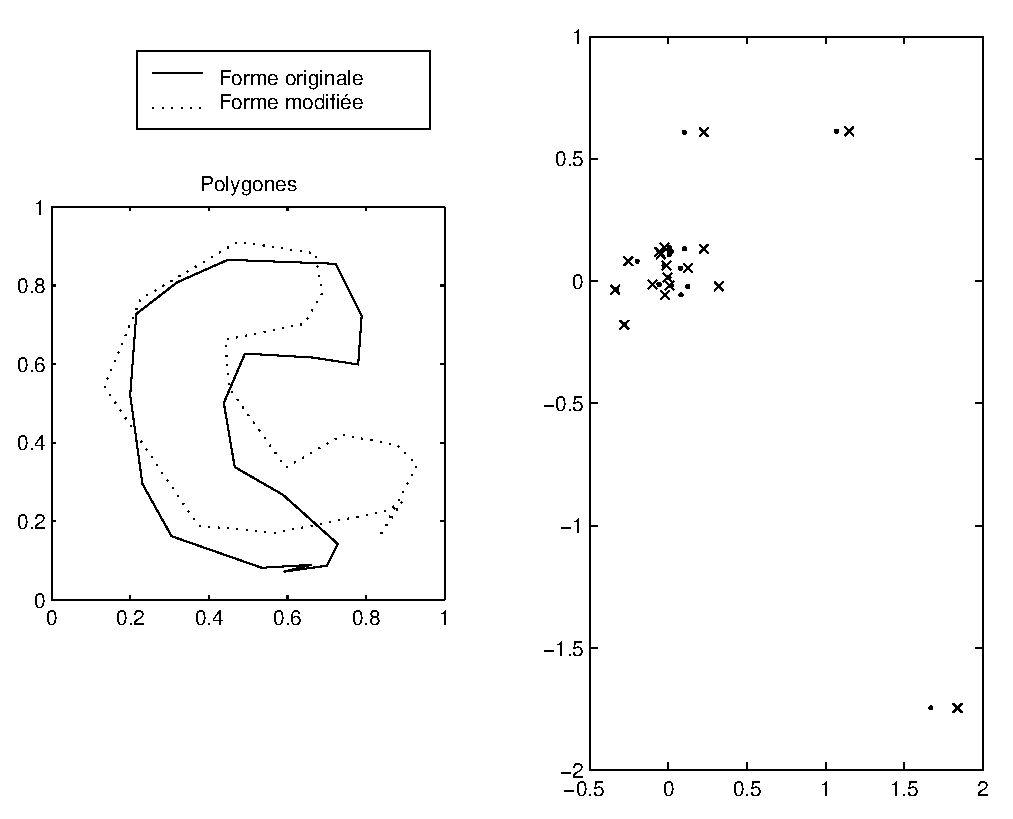
\includegraphics[scale=0.6]{images/fourier-descriptors.eps}
    \end{center}
    \caption{Fourier descriptors for two similar forms}
              \label{fig-fourier-descriptors}
\end{figure}
 
 
 
From a practical point of view, the numerical computation of the solution of an equation can, at various times of the discretization process, lead to the use of the discrete Fourier transform. This can come from a pure and simple discretization of the continuous Fourier transform (for example for \textit{the heat equation}, paragraph \ref{sect2-resol-eq-heat}), or from a more ingenious way to simplify and speed up calculations (for example for \textit{Poisson's equation}, paragraph \ref{sect2-resol-eq-Poisson}). In the following paragraphs, we will focus on these numerical aspects; The theoretical use of the continuous transform is detailed in particular in the exercise \oldref{exo-unicite-eq-heat}.

% ------------------------------------------------- -----
% ------------------------------------------------- -----
% sub-section - Calculation of Fourier coefficients                            
% ------------------------------------------------- -----
% ------------------------------------------------- -----
\subsection{Calculation of Fourier coefficients}
\label{sect2-calcul-coef-fourier} 
 
 
\index{Fourier coefficient!calculation by FFT} As we saw in paragraph \ref{sect2-calculus-trans-fourier-approach}, the FFT algorithm allows to calculate in an approximate way the value of the Fourier transform continue at certain frequencies $ \xi_k $. But in reality, the calculation of $ \wh{f}[\xi_k] $ that we carried out corresponds to the approximation of the integral:
\begin{equation}
\label{eq-lien-fft-calcul-coef-fourier}
\wh{f} (\xi_k) \approx \Delta \int_{0}^{N \Delta}{f(t) e^{- \frac{2 \imath \pi}{N \Delta} kt} \d t}.
\end{equation}
Now, if we denote by $ f_1 $ the periodic function of period $ N \Delta $ which coincides with $ f $ on the interval $ [0, \, N \Delta] $, the equation \eqref{eq-lien-fft-calcul-coef-fourier} corresponds to the calculation of $ c_k (f_1) $, the $ k^{ieme} $ Fourier coefficient of the function $ f_1 $.
 
 
Let us summarize all these results by a formula allowing to calculate in an approximate way $ N $ Fourier coefficients for a periodic function $ f $ of period $ 1 $:
\begin{equation*}
\forall n \in \{-N / 2 + 1, \ldots, \, 0, \ldots, \, N / 2 \}, \quad c_n (f) \eqdef \int_0^1{f(t) e^{- 2 \imath \pi nt} \d t} \approx \frac{1}{N} \wh{f}[n],
\end{equation*}
where we denote by $ \wh{f} $ the transformed Fourier vector of the vector $ \{f(k / N) \}_{k = 0}^{N-1} $.
 
 
The FFT algorithm will therefore allow the calculation of $ N $ Fourier coefficients of a function sampled in $ N $ points all at once. Moreover, the techniques of adding zeros and refining the sample make it possible to modulate the number of coefficients calculated for the same sample. The only potential problem lies in the lack of precision (the rectangle method is only of order 1), which can be problematic when the Fourier coefficients decrease rapidly towards 0, as is the case for a very regular function. Two solutions are then possible: \begin{rs}
\item increase the number of interpolation points.
\item use a higher integration method. It is possible to show a discrete Fourier transform with formulas other than that of rectangles (for example that of \textit{Simpson}). The exercise \oldref{exo-calcul-approaches-transfo-frac}, question 2, details this technique.
\end{rs}
% ------------------------------------------------- -----
% ------------------------------------------------- -----
% sub-section - Application to the heat equation                            
% ------------------------------------------------- -----
% ------------------------------------------------- -----
\subsection{Application to the heat equation}
\label{sect2-resol-eq-heat} 
 
 
\index{Fourier@\nompropreindex{Fourier}} In this paragraph, we will apply the method described in the previous paragraph, which allows us to calculate all at once a very large number of Fourier coefficients (admittedly with questionable precision). It is a question of solving the heat equation, which historically had a very important role, since it was this which pushed \nompropre{Joseph Fourier} to develop his theory, in his article \textit{Theorie Analytique de the Heat} (1822).
 
 
\index{Equation!of heat} We want to solve in an approximate way the equation of heat on the circle $ S^1 \eqdef \RR / \ZZ $:
\begin{equation}
\label{heat-eq}
\left\{\begin{array}{l} \forall (t, \, x) \in \RR_*^{+} \times S^1, \quad \displaystyle{\pd{u}{t} = \kappa \pdd{u}{x}} \\\forall x \in S^1, \quad u (0, \, x) = f(x) \end{array} \right. ,
\end{equation}
where the sought solution $ u $ is assumed to be sufficiently regular over $ \RR_*^{+} \times S^1 $, and continues over $ \RR^{+} \times S^1 $. In this paragraph, we are not going to use a finite difference method, unlike what we will do in the \ref{sect2-resol-eq-Poisson} paragraph to solve the Poisson equation. The exercise \oldref{exo-resol-eq-heat-diff-finies} studies the stability of such a method for the heat equation. Instead, we will explicitly solve the continuous equation, and calculate approximations of the solution by FFT.
 
 
This equation reflects the evolution of heat in a circle of length 1, completely isolated, and of which we know the initial temperature distribution. The constant $ \kappa $ translates the conductivity of the material, and without loss of generality, it will be taken equal to $ \frac{1}{2} $ in the following. Indeed, we can replace the function $ u $ by $ (t, \, x) \mapsto u \left(\frac{t}{2 \kappa}, \, x \right) $, which does not modify the problem. For an exposition on the different applications of series and the Fourier transform to differential equations (and in particular to the heat equation), the book of \nompropre{Dym} and \nompropre{MacKean} \cite{dym} is an excellent source. In the following, we will content ourselves with stating the main results. In particular, the uniqueness result is detailed in the exercise \oldref{exo-unicite-eq-heat}.
 
 
\index{Fourier!series} To begin with, we are looking for a formal solution in the form
\begin{equation*}
u (t, \, x) \eqdef \sum_{n \in \ZZ}{c_n (t) e_n (x)} \quad \quad \text{with} \quad e_n (x) \eqdef e^{2 \imath \pi nx},
\end{equation*}
since intuitively, the solution must be periodic at $ t $ fixed. The coefficients $ c_n (t) $ are defined by
\begin{equation*}
\forall t> 0, \quad c_n (t) \eqdef \int_0^1{u (t, \, x) e_n (-x)} \d x.
\end{equation*}
By doing two integrations by parts, we obtain a differential equation verified by $ c_n $:
\begin{equation*}
\begin{split}
\frac{d c_n}{dt} (t) = & \int_0^1{\pd{u}{t} (t, \, x) e_n (-x) \d x} = \int_0^1{\frac{1}{2} \pdd{u}{x} (t, \, x) e_n (-x) \d x} \\
= & - 2 \pi^2 n^2 \int_0^1{u (t, \, x) e_n (-x) \d x} = -2 \pi^2 n^2 c_n (t).
\end{split}
\end{equation*}
As $ c_n (0) = \wh{f} (n) $ (the \ordin{n}{th} Fourier coefficient of $ f $), we obtain a formal solution of the heat equation \eqref{heat-eq}:
\begin{equation}
\label{eq-solution-heat-equation}
\forall (t, \, x) \in \RR_*^{+} \times S^1, \quad u (t, \, x) = \sum_{n \in \ZZ}{\wh{f} (n) \exp (-2 \pi^2n^2 t) e_n (x)}.
\end{equation}
The fact that the function $ u $ thus defined is indeed the solution of the problem posed for $ t> 0 $ comes from the fact that we can differentiate under the sum sign because the series of terms $ \exp (-2 \pi^2n^2 t) $ is normally convergent for $ t \geq \epsilon> 0 $, as well as all its derivatives with respect to $ t $. The only thing difficult to show is that we have
\begin{equation*}
\norm{u (t, \, \cdot) - f}_{\infty} \tv{t \to 0} 0,
\end{equation*}
that is to say that the initial conditions are well respected. We recall that $ \norm{\cdot}_\infty $ denotes the uniform norm over $ S^1 $. All this is detailed in the exercise \oldref{exo-unicite-eq-heat} at the same time as the proof of the uniqueness of the solution.
 
\begin{rem}{(\upshape \textbf{Continuous filtering}).} 
\index{Filter!continuous} \index{Gaussian} Intuitively, the passage from $ u (0, \, \cdot) = f $ to $ u (t, \, \cdot) $ corresponds to the multiplication of the coefficients of Fourier $ \wh{f} (n) $ of $ f $ by $ \exp (-2 \pi^2n^2 t) $. This amounts to filtering $ f $ by a Gaussian, that is to say to smooth the starting function. The larger $ t $, the greater the variance of the Gaussian, and therefore the more pronounced the blurring effect induced by the filtering. Ultimately, when $ t \rightarrow + \infty $, the filtering simply corresponds to averaging the function, so the heat distribution is uniform.
\end{rem}
 
 
 
In order to approximate the solution $ u $ of the heat equation, we will, for some fairly large $ N $ fixed (which we assume to be a power of 2), calculate
\begin{equation*}
u_N (t, \, x) \eqdef \sum_{n = -N / 2}^{N / 2-1}{c_n (t) e_n (x)}.
\end{equation*}
\index{Matlab@\Matlab{}} Of course, we will use the technique developed in paragraph \ref{sect2-calcul-coef-fourier} and therefore sample the function $ f $ according to a vector $ \wt{f} \eqdef \{f(k / n) \}_{k = 0}^{N-1} $. The calculation of the FFT of this vector allows us, up to a factor $ \frac{1}{N} $, to calculate approximately $ N $ Fourier coefficients of the function $ f $, and therefore to construct the function $ u_N $. All this is detailed in the \Matlab{} programs presented in the \annexeref{sect1-listing-heat} paragraph. The only technical difficulty is that the Fourier coefficients calculated by the FFT are not arranged in the right order, but via the indexing $ \{0, \ldots, \, N / 2-1, \, -N / 2 , \ldots, \, -1 \} $. We can see the evolution of the solution over time in the figure \figref{fig-eq-heat-evolution}, where the initial data is an indicator function (therefore discontinuous). We can clearly see the regularizing effect of the heat equation: for $ t> 0 $, the solution becomes smooth, and tends towards a constant function when $ t $ tends towards $ + \infty $. \begin{figure}[ht]
    \begin{center}
    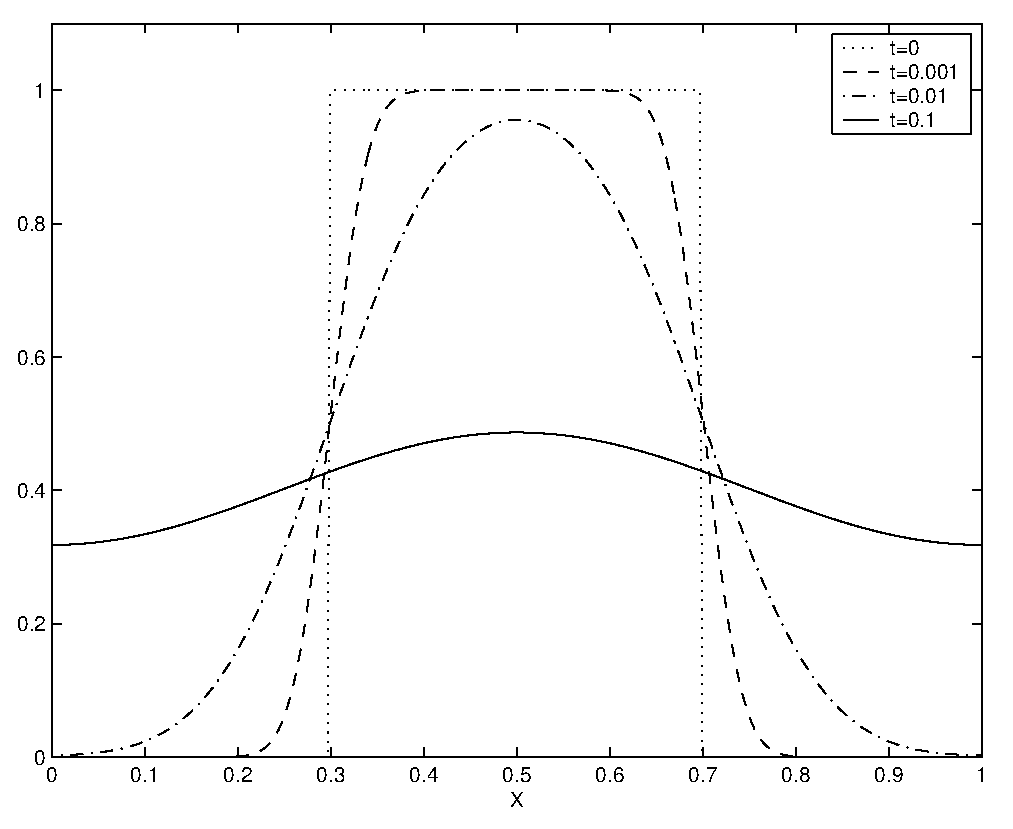
\includegraphics[scale=0.4]{images/eq-chaleur-evolution.eps}
    \end{center}
    \caption{Evolution of the solution of the heat equation}
              \label{fig-eq-heat-evolution}
\end{figure}
 
 
\begin{rem}{(\upshape \textbf{Discrete filtering}).} 
\index{Filter!discrete} Solving the heat equation by DFT therefore amounts to performing a discrete filtering with an increasingly strong low-pass filter. In essence, filtering through a symmetrical low pass filter amounts to solving the heat equation for a certain time $ t $. The more the filter is regularizing, the greater $ t $.
\end{rem}
 
% ------------------------------------------------- -----
% ------------------------------------------------- -----
% sub-section - Solving the Poisson equation by finite differences                            
% ------------------------------------------------- -----
% ------------------------------------------------- -----
\subsection{Solving the Poisson equation by finite differences}
\label{sect2-resol-eq-Poisson} 
 
 
\index{Poisson's equation} \index{Poisson@\nompropreindex{Poisson}} We want to find a function $ u: [0, \, 1] \times [0, \, 1] \rightarrow \RR $ sufficiently regular (of class $ \Cc^2 $) which satisfies the equation of \textit{Poisson}:
\begin{equation}
\label{eq-fish}
\left\{\begin{array}{l} \forall (x, \, y) \in [0, \, 1] \times [0, \, 1], \quad \displaystyle{\Delta u (x , \, y) \eqdef \pdd{u}{x} + \pdd{u}{y} = f(x, \, y)} \\\forall x \in [0, \, 1], \quad u (x, \, 0) = u_{x0} (x) \quad \text{and} \quad u (x, \, 1) = u_{x1} (x) \\\forall y \in [ 0, \, 1], \quad u (0, \, y) = u_{0y} (y) \quad \text{and} \quad u (1, \, y) = u_{1y} (y) \end{array} \right.
\end{equation}
where $ f: \RR^2 \rightarrow \RR $ is a continuous function known in advance, and the functions $ u_{x0} $, $ u_{x1} $, $ u_{0y} $ and $ u_{1y} $ are also supposedly known continuous functions (we fix the values of the solution on the edges).
 
 
The equation of \textit{Poisson} has very important interpretations, especially in physics. We can note: \begin{rs}
\item \index{Elastic membrane} \textit{equation of an elastic membrane}: the surface of the membrane is represented by the equation $ z = u (x, \, y) $. The function $ f $ represents the surface amount of forces applied vertically to the surface. Imposing the value of the function $ u $ on the edges corresponds to fixing the edges of the surface to a reinforcement.
\item \index{Electric potential} \textit{equation of an electric potential}: the quantity $ u (x, \, y) $ represents the value of a surface electric potential at a point $ (x, \, y ) $, and the function $ f $ takes into account a surface distribution of electric charges.
\end{rs} \index{Laplace's equation} \index{Laplace@\nompropreindex{Laplace}} \index{Function!harmonic} \index{Difference!finite} In the particular case where the function $ f $ is zero , we speak of the equation of \textit{Laplace}, and the function $ u $ is then called \textit{harmonic function}. Obviously, we show that the real part of a holomorphic function is harmonic. We can even show that locally, the converse is true (and therefore a harmonic function has partial derivatives at any order!). For more details on the theory of harmonic functions, one can consult the book of \nompropre{Rudin} \cite [p.275]{rudin}.
 
 
We propose to approach the solution $ u $ of the equation \eqref{eq-fish} by the method of \textit{finite differences}. To do this, we will discretize the square $ [0, \, 1] \times [0, \, 1] $ according to $ N + 1 $ points on both directions. We therefore seek an approximate solution $ \{U (i, \, j) \}_{0 \leq i, \, j \leq N} $, where $ U (i, \, j) $ represents an approximation of $ u (ih, \, jh) $ (we noted $ h \eqdef \frac{1}{N} $ the step of the subdivision). By replacing the Laplacian $ \Delta u $ by a discrete approximation, we obtain, for the interior squared points, the following equations, for $ i $ and $ j $ in $ \{1, \ldots, \, N-1 \} $,
\begin{equation}
\label{eq-poisson-discretise}
\frac{1}{h^2} \left\{U (i-1, \, j) + U (i + 1, \, j) + U (i, \, j + 1) + U (i , \, j-1) - 4 U (i, \, j) \right\} = F (i, \, j),
\end{equation}
where we denote by $ F (i, \, j) \eqdef f(ih, \, jh) $ the right side of the equation. We have of course paid attention to the boundary terms ($ i, \, j = 0, \, N $), which are not part of the system since they are fixed once and for all by the boundary conditions.
 
 
\index{Filtering} \index{Filter} We would thus be tempted to write the equation \eqref{eq-poisson-discretise} as a convolution by a filter $ \Phi $:
\begin{equation*}
U * \Phi = F
\end{equation*}
\index{Convolution!2D} where $ * $ denotes the 2D circular convolution operator, defined in paragraph \ref{sect2-convolution-2d}, and the transfer function is written
\begin{equation}
\label{eq-filter-eq-fish}
\Phi \eqdef \frac{1}{h^2} \begin{pmatrix} 1 & & & \\& & \vdots & \\& \ldots & 0 & \ldots \\& & \vdots & \\1 & & & \\-4 & 1 & & 1 \\\end{pmatrix},
\end{equation}
(it should be remembered that the functions considered are N periodic, so that the negative frequencies are pushed to the other end of the table). However, there are at least two objections to this writing. \begin{rs}
\item The filters operate on a periodic signal, but this is not the case here: the values of the edges have no reason to \guill{re-stick}. Moreover, the equation \eqref{eq-poisson-discretise} is only valid inside the domain, that is to say for $ 0 <i, \, j <N $. It does not describe a circular convolution.
\item The edge values are taken into account in the filtering, so they are part of the unknowns: on the contrary, we want them to be fixed.
\end{rs} To work around this problem, it suffices to make null $ U $ at the ends, that is to say for $ i, \, j = 0, \, N $, quite simply by passing in the right-hand side the edge terms. Here is for example an equation obtained for $ i = 1 $ and $ 1 <j <N-1 $:
\begin{equation*}
\begin{split}
\frac{1}{h^2} \left\{0 + U (2, \, j) + U (1, \, j + 1) + U (1, \, j-1) - 4 U ( 1, \, j) \right\} & = F (i, \, j) - \frac{1}{h^2} u_{0y} (jh) \\
& \eqdef \wt{F} (i, \, j),
\end{split}
\end{equation*}
(we used the fact that $ U (0, \, j) = u_{0y} (jh) $ the value fixed on the edge $ x = 0 $). By doing the same for the four edges of the matrix $ F $, we create a new matrix $ \wt{F} $ zero on the edges, and thanks to this manipulation, we can replace the unknown $ U $ by an unknown $ \wt{U} $ which is zero on the edges. It remains precisely to solve the problem of the application of the filter on the edges (the equation \eqref{eq-poisson-discretise}) is only valid inside). To be able to do this, it suffices to extend the functions considered by imparity along the two axes. Indeed, the nullity of the function on the edges as well as the equation \eqref{eq-poisson-discretise} of the filter shows that the terms symmetrical with respect to an edge must be of opposite signs. For example, we have the equation
\begin{equation*}
U (1, \, j) + U (-1, \, j) = \wt{F} (0, \, j) = 0,
\end{equation*}
hence $ U (1, \, j) = - U (-1, \, j) $. We therefore extend the matrices $ \wt{U} $ and $ \wt{F} $ to obtain matrices (always noted in the same way) of size $ 2 N $ odd. Thus, in the (simplistic, but instructive) case where $ N = 3 $, the matrix $ \wt{F} $ will be written
\begin{equation*}
\wt{F} = \begin{pmatrix} 0 & 0 & 0 & 0 & 0 & 0 \\0 & \wt{F} (1, \, 1) & \wt{F} (2, \, 1 ) & 0 & - \wt{F} (2, \, 1) & - \wt{F} (1, \, 1) \\0 & \wt{F} (1, \, 2) & \wt{F} (2, \, 2) & 0 & - \wt{F} (2, \, 2) & - \wt{F} (1, \, 2) \\0 & 0 & 0 & 0 & 0 & 0 \\0 & - \wt{F} (1, \, 2) & - \wt{F} (2, \, 2) & 0 & \wt{F} (2, \, 2) & \wt{F} (1, \, 2) \\0 & - \wt{F} (1, \, 1) & - \wt{F} (2, \, 1) & 0 & \wt{F} (2, \, 1) & \wt{F} (1, \, 1) \\\end{pmatrix}.
\end{equation*}
With all these new conventions, the equation \eqref{eq-poisson-discretise}, which extends to $ 0 \leq i, \, j \leq 2N $ and is also true as a periodic convolution, is written
\begin{equation*}
\wh{U} * \wt{\Phi} = \wt{F},
\end{equation*}
where $ \wt{\Phi} $ is still defined as in the equation \eqref{eq-filter-eq-fish}, but this time is of size $ 2 N $.
 
 
The idea is then to take the 2D Fourier transform of the two members, since the latter transforms the convolution product into a simple product, as stated in the proposition \ref{sect1-tfd-prod-convol}. We get the very nice equation
\begin{equation*}
\Ff \left(\wt{U} \right) \cdot \Ff \left(\wt{\Phi} \right) = \Ff \left(\wt{F} \right),
\end{equation*}
where we denote by $ \cdot $ the term-to-term product of the two matrices. This equation is now very easy to solve, since we know how to calculate the transform of $ \wt{\Phi} $, as shown by the following lemma.
 
\begin{lem}
The Fourier transform of the transfer function $ \Phi $ is given by
\begin{equation*}
\Ff \left(\wt{\Phi} \right) = - \frac{4}{h^2} \left\{\sin \left(\frac{i \pi}{2N} \right)^2 + \sin \left(\frac{j \pi}{2N} \right)^2 \right\}_{0 \leq i, \, j \leq 2N-1}.
\end{equation*}
\end{lem}
\begin{proofnoqed}
It is enough to apply the definition and to make a grouping of terms:
\begin{align*}
\Ff \left(\wt{\Phi} \right) [i, \, j] & = \sum_{k, \, l}{\Phi [k, \, l] e^{\frac{2 \imath \pi}{2N} ki} e^{\frac{2 \imath \pi}{2N} lj}} \\
& = \frac{1}{h^2} \left\{e^{\frac{2 \imath \pi}{2N} i} + e^{\frac{2 \imath \pi}{2N} j} + e^{- \frac{2 \imath \pi}{2N} i} + e^{- \frac{2 \imath \pi}{2N} j} - 4 \right\} \\
& = - \frac{4}{h^2} \left\{\sin \left(\frac{i \pi}{2N} \right)^2 + \sin \left(\frac{j \pi}{2N} \right)^2 \right\}. \tag*{\qed}
\end{align*}
\end{proofnoqed}
So we get
\begin{equation*}
G (i, \, j) = \Ff \left(\wt{U} \right) (i, \, j) = \frac{\Ff(\wt{F}) (i, \, j)}{\sin^2 \left(\frac{i \pi}{2N} \right) + \sin^2 \left(\frac{j \pi}{2N} \right)},
\end{equation*}
(be careful with the division $ 0 / $ 0 for $ i = j = $ 0, but we know that the result is 0). We finish thanks to the calculation of the inverse transform, $ \wt{U} = \Ff^{-1} (G) $. It only remains to extract the part of the matrix $ \wt{U} $ that interests us (that is to say $ 0 \leq i, \, j \leq N $), and to add the terms that we had cut off at the beginning.
 
 
\index{Matlab@\Matlab{}} The entirety of this method to solve the Poisson equation is taken algorithmically in \Matlab{} in the paragraph \annexeref{sect1-listing-fish}. To be able to observe the quality of the approximation, we chose an equation for which we know the solution (in fact, we first choose the solution, then we calculate the right hand side), and we create the boundary functions accordingly . Figure \figref{fig-eq-fish} shows the solution of a Poisson equation for which we explicitly know a solution, namely $ u (x, \, y) = e^{xy} $. The figure \figref{fig-eq-Poisson-modif} uses the same equation, but modifies the conditions on two of the edges. 

\begin{figure}[ht] 
\begin{minipage}{0.5 \linewidth}
    \begin{center}
    \includegraphics [scale = 0.3]{images/eq-poisson.eps}
    \caption{Solution of the Poisson equation}
              \label{fig-eq-fish}
    \end{center}
\end{minipage}
\begin{minipage}{0.5 \linewidth}
    \begin{center}
    \includegraphics [scale = 0.3]{images/eq-poisson-modif.eps}
    \caption{Solution modified}
              \label{fig-eq-Poisson-modif}
    \end{center}
\end{minipage}
\end{figure}
 
 
\begin{rem}{(\upshape \textbf{Case of a quadratic functional}).} 
\index{Function!quadratic} If we consider an exact quadratic solution, for example the function $ u (x, \, y) = x^2 + y^2 $, which satisfies the Poisson equation:
\begin{equation*}
\pdd{u}{x} + \pdd{u}{y} = 4,
\end{equation*}
one notices that the error obtained during the resolution by a finite difference method is quasi-zero. This is explained by the fact that the approximation of the Laplacian by the equation \eqref{eq-poisson-discretise} is in fact exact for a polynomial of degree less than two (it is an interpolation formula of order of them).
\end{rem}
The exercise \oldref{exo-formulation-matrix-fish} takes up this method of resolution by explaining its operation by matrix decompositions.

% ------------------------------------------------- -----
% ------------------------------------------------- -----
% ------------------------------------------------- -----
% section - Product calculations                            
% ------------------------------------------------- -----
% ------------------------------------------------- -----
% ------------------------------------------------- -----
\section{Product calculations}
% \addcontentsline{toc}{section}{Product calculations}
\label{sect1-calculations-products} 
 
 
\index{Calculation!of products} Contrary to what one might think after all these applications dedicated to numerical calculation, the FFT algorithm has applications of a much more algebraic nature. It is mainly the convolution property that is used. This algorithm allowed significant advances for certain arithmetic calculations, for example for intensive calculations of large numbers (the search for decimals of $ \pi $ is the best example). We can read about this subject \cite{bailey-pi} which explains some instructive anecdotes.
% ------------------------------------------------- -----
% ------------------------------------------------- -----
% sub-section - Theoretical presentation                            
% ------------------------------------------------- -----
% ------------------------------------------------- -----
\subsection{Theoretical presentation}
\label{sect2-presentation-theoretical} 
 
 
Before describing methods using the FFT algorithm presented in paragraph \ref{sect2-present-algo-fft}, to calculate products, we can explain in a somewhat theoretical way the approach we are going to follow.
 
 
\index{Kernel} \index{Morphism} \index{Ideal} Consider, for $ (\xi_0, \ldots, \, \xi_{N-1}) \in \CC^N $, the evaluation morphism
\begin{equation*}
\Phi: \func{\CC [X]}{\CC^N}{P}{\left(P (\xi_0), \ldots, \, P (\xi_{N-1}) \right)} .
\end{equation*}
The kernel of this morphism is the ideal of $ \CC [X] $ generated by the polynomial $ \prod_{k = 0}^{N-1}{(X- \xi_k)} $. In the case where the points $ \xi_k $ are distinct, we obtain, by passing to the quotient, a linear isomorphism (since the two spaces have the same dimension $ N $)
\begin{equation*}
\wt{\Phi}: \left\{\begin{array}{ccc} \CC [X] / \prod_{k = 0}^{N-1}{(X- \xi_k)} & \xrightarrow{\simeq} & \CC^N \\\ol{P} & \mapsto & (\ol{P} (\xi_0), \ldots, \, \ol{P} (\xi_{N-1})) \end{array} \right. .
\end{equation*}
It is even evidently an isomorphism of algebra, if we endow $ \CC [X] $ with the product of the polynomials, and $ \CC^N $ with the product component by component.
 
 
Thanks to this evaluation morphism, and its inverse morphism (interpolation), we can draw the following diagram:
\begin{equation*}
\begin{CD} (P_0, \ldots, \, P_{N-1}), (Q_0, \ldots, \, Q_{N-1}) @> mult.polyn \hat{o} mes> \grdo (N^2)> (R_0, \ldots, \, R_{N-1}) \\@VV{\acute{e} valuation} V @A{interpolation} AA \\\begin{array}{l} (P (\xi_0), \ldots, \, P (\xi_{N-1})), \\(Q (\xi_0), \ldots, \, Q (\xi_{N-1})) \end{array} @>{one-time mult.}>{\grdo (N)}> (R (\xi_0), \ldots, \, R (\xi_{N-1})) \end{CD},
\end{equation*}
which suggests a new way to multiply two polynomials, passing \guill{downwards}, namely using the application
\begin{equation*}
\Psi: \func{\CC [X] \times \CC [X]}{\CC [X] / \prod{(X- \xi_k)}}{(P, \, Q)}{\Phi^{-1} (\Phi (\ol{P}) \cdot \Phi (\ol{Q}))},
\end{equation*}
where we denote by $ \ol{P} $ the class of $ P $ in the algebra $ \CC [X] / \prod{(X- \xi_k)} $. From what we have just said, this morphism therefore calculates the product of the two polynomials modulo the polynomial $ \prod{(X- \xi_k)} $. The natural questions are therefore the following. \begin{rs}
\item What choice to make for the points $ \{\xi_0, \ldots, \, \xi_{N-1} \} $ so that this new way of calculating a product is fast?
\item How to really get the product of the two polynomials, and not just the product modulo a certain polynomial?
\end{rs} In fact, we have already answered these two questions in chapter \oldref{chap-tfd}. It suffices to link the TFD to the evaluation of polynomials to reinvest the algorithms already constructed.
 
\begin{rem}
\index{Chinese!Lemma} The $ \wt{\Phi} $ isomorphism is in fact the canonical isomorphism given by the Chinese theorem:
\begin{equation*}
\CC [X] / \prod_{k = 0}^{N-1}{(X- \xi_k)} \xrightarrow{\simeq} \prod_{k = 0}^{N-1}{\CC [ X] / (X- \xi_k)} \simeq \CC^N.
\end{equation*}
Indeed, the $ X- \xi_k $ are prime among themselves (because the $ \xi_k $ are distinct), therefore the application of the theorem is licit, and the reduction modulo $ X- \xi_k $ sends a polynomial $ P $ on $ P (\xi_k) $.
\end{rem}
 
% ------------------------------------------------- -----
% ------------------------------------------------- -----
% sub-section - Multiplication of polynomials modulo $ \mbold{X^N-1} $                            
% ------------------------------------------------- -----
% ------------------------------------------------- -----
\subsection{Multiplication of polynomials modulo $ \mbold{X^N-1} $}
\label{sect2-multiplication-polynomials-modulo-xn-1} 
 
 
\index{Polynomial!multiplication} \index{Product!of polynomials} The aim of this paragraph is to present the Fourier transform as a transformation (in fact a morphism) on polynomials of fixed degrees. We can then use the algebraic properties of the discrete Fourier transform as well as the FFT algorithm to perform operations on polynomials very quickly. Behind these particularly efficient methods hides a more subtle problem than the simple use of the Fourier transform, since it is the question of the representation of polynomials. Indeed, the Fourier transform makes it possible to juggle between two types of representations, and thus to exploit the strengths of each.
 
 
The purpose of this approach being to reinvest the algorithms already presented in chapter \oldref{chap-tfd} (mainly FFT and fast convolution), we hasten to choose wisely the points of evaluation / interpolation $ \xi_k $, by l' occurrence, the $ N $ roots \ordin{N}{iès} of the unit, i.e. $ \xi_k = \omega_N^{- k} = e^{- \frac{2 \imath k \pi}{N}} $ for $ k = 0, \ldots, \, N-1 $. We see then that the morphism $ \wt{\Phi} $ is in fact the discrete Fourier transform. More precisely, we can rewrite it as follows:
\begin{equation*}
\wt{\Phi}: \left\{\begin{array}{ccc} \CC [X] / (X^N-1) & \xrightarrow{\simeq} & \CC^N \\\ol{P} & \mapsto & \wt{\Phi} (P) = \Ff(P_0, \ldots, \, P_{N-1}) \end{array} \right.,
\end{equation*}
where we denote by $ P_0, \ldots, \, P_{N-1} $ the coefficients of the polynomial $ \ol{P} $ (we have chosen the representative of degree less than $ N $). Of course, we used the identity $ \prod_{k = 0}^{N-1}{(X- \xi_k)} = X^N-1 $ here. We therefore notice that the computation of the discrete Fourier transform of $ P $ (as a vector of $ \CC^N $) is nothing other than the computation of the values that $ P $ takes in them. $ N $ roots \ordin{N}{ièmes} of the unit, and we find exactly the morphism $ \Phi $ of the previous paragraph.
 
 
The discrete Fourier transform thus makes it possible to juggle between two representations of polynomials of degree $ N-1 $ (in fact modulo $ X^N-1 $): \begin{rs}
\item \index{Representation!by coefficients} \textit{representation by coefficients}: this amounts to considering a polynomial as a vector of $ \CC^N $. Although very commonly used, this representation has a weak point: it is not at all suitable for calculating the product of two polynomials. While the sum of two polynomials $ P $ and $ Q $ of degree at most $ N $ is calculated in $ N $ operations (as shown by the equality $ (P + Q)_k = P_k + Q_k $), the product, calculated naively, requires $ N^2 $ operations.
\item \index{Representation!by values} \textit{representation by values}: we give ourselves the polynomial by the values it takes in $ N $ distinct points (here taken in a very particular way, the roots \ordin{N}{ith} of the unit). This representation is much more suited to the computation of the product, since it suffices to do the product of the values of each polynomial.
\end{rs} Take this literally: the FFT algorithm provides a quick and easy way to switch between representations.
 
 
To finish, let us recall the equation obtained for the computation of the product of two polynomials modulo $ X^N-1 $:
\begin{equation}
\label{eq-prod-cyclic-polynomial}
P * Q = \Ff^{-1} \left(\Ff(P) \cdot \Ff(Q) \right).
\end{equation}
\index{Convolution!circular} In this equation, we have confused vector and modulo polynomials $ X^N-1 $, and the product $ P * Q $ can also be seen as a product of circular convolution between two vectors. The operation performed can be graphically represented. The first two graphs in figure \figref{fig-convolution-polynomial} show the polynomials defined by $ P = 1 + 2X + X^3-X^4 + X^5 $ as well as $ Q = XX^2 + 2X^3 + 2X^5$. On the abscissa, we put the degrees of monomials $ 1, \ldots, \, X^{10} $. We therefore choose to work in $ \ZZ/11 \ZZ $. This makes sense, because the degree of the product $ P * Q $ is precisely $ 10 $. Thus, when we represent in the graph on the right the product of the two vectors, we find the graphical representation of the product $ P * Q $, since the reduction modulo $ X^{11} -1 $ did not have effect. \begin{figure}[ht]
    \begin{center}
    \includegraphics[scale=0.7]{images/convolution-polynome.eps}
    \end{center}
    \caption{Graphical representation of the product of polynomials by convolution}
              \label{fig-convolution-polynomial}
\end{figure}
 
 
\begin{rem}{(\upshape \textbf{Lagrange interpolation}).} 
Algorithms make it possible to calculate the interpolation polynomials in the case where the points $ \xi_k $ are not necessarily roots of the unit. There is of course the result of \textit{Lagrange}, which gives an explicit basis of $ \CC_{N-1}[X] $ (space of polynomials of degree at most $ N-1 $) in which the computation is done simply. Indeed, if we look for the polynomial $ P $ which takes the values $ y_i $ at the points $ x_i $, for $ i = 0, \ldots, \, N-1 $, then $ P = \sum_{i = 0}^{N-1}{y_i P_i} $, where $ P_i $ is the \ordin{i}{rd} \textit{Lagrange polynomial} associated with the points $ \{x_i \}_{i = 0}^{N-1} $:
\begin{equation*}
P_i \eqdef \frac{\prod_{j = 0}^{N-1} (X-x_j)}{\prod_{j \neq i} (x_i-x_j)}.
\end{equation*}
\index{Difference!divided} \index{Lagrange!polynomial} However, the numerical computation of the interpolation polynomial in the base of $ \{P_i \}_{i = 0}^N $ is not used in practice, because it leads to an accumulation of numerical errors. We prefer to use the \textit{divided differences} technique, which is explained for example in \cite{demailly}.
\end{rem}
 
% ------------------------------------------------- -----
% ------------------------------------------------- -----
% sub-section - Multiplication of polynomials                            
% ------------------------------------------------- -----
% ------------------------------------------------- -----
\subsection{Multiplication of polynomials}
\label{sect2-multiplication-polynomials} 
 
 
The difficulty with which we are faced when calculating the product of two polynomials $ P $ and $ Q $ (of degree $ N-1 $) by the method presented above is that a priori, the product $ PQ $ is a polynomial of degree $ 2N-2 $. This polynomial will therefore be reduced modulo $ X^N-1 $, which often has a more than undesirable effect ... More precisely, the coefficients of the product are given by the equation
\begin{equation}
\label{eq-product-polynomials}
\forall n \in \{0, \ldots, \, 2 N - 1 \}, \quad (PQ)_n = \sum_{k = 0}^{n}{P_k Q_{n - k}}.
\end{equation}
\index{Convolution!acyclic} It is in fact an acyclic convolution product (to be compared to the cyclic product of the equation \eqref{eq-prod-cyclic-polynomial}), and we will be able to use the technique already presented in the Section~\ref{sect1-convolution-acyclic}, to calculate it.
 
 
\index{Convolution!circular} This approach (adding zeros at the end of the vector to make the product cyclic) is very intuitive, since it consists in considering the two polynomials as polynomials of degree $ 2N-1 $ (by adding zero coefficients). We can then apply the approach presented in the previous paragraph (ie use a cyclic convolution product, or if you prefer, calculate the product modulo $ X^{2N} -1 $). Fortunately, this does not change the result, since the polynomial $ PQ $ is not affected by the reduction modulo $ X^{2N} -1 $. In a more theoretical way, this amounts to using the bijectivity of the application
\begin{equation*}
\func{\CC_{2N-1}[X]}{\CC [X] / (X^{2N} - 1)}{P}{P \mod{X^{2N} - 1}},
\end{equation*}
where we denote by $ \CC_{2N-1}[X] $ the space of polynomials of degree less than or equal to $ 2N-1 $.
% ------------------------------------------------- -----
% ------------------------------------------------- -----
% sub-section - Multiplication of large integers                            
% ------------------------------------------------- -----
% ------------------------------------------------- -----
\subsection{Multiplication of large integers}
\label{sect2-multiplication-integers} 
 
 
\index{Integer!multiplication} \index{Calculation!of products of integers} \index{Product!of integers} We denote by $ (a_0, \ldots, \, a_{N-1}) $ the base representation $ b $ of a large integer $ a $, that is
\begin{equation*}
a = a_0 + a_0 b + \cdots + a_{N-1} b^{N-1}.
\end{equation*}
\index{Matlab@\Matlab{}} We notice that the multiplication of two integers $ a $ and $ a'$ is similar to the calculation of a product of polynomials, with one exception: the integers $ a_k $ and $ a'_k $, for $ k = 0, \ldots, \, N-1 $, must belong to the set $ \{0, \ldots, \, b-1 \} $. If we want to quickly compute the multiplication of two large integers, we can therefore use the polynomial product technique that we have just exposed in the previous paragraph, followed by a \guill{carry propagation} phase. \Matlab{} programs allowing to achieve all this are gathered in the paragraph \annexeref{sect1-listing-mult-integers}.
 
 
This approach nevertheless suffers from some weak points, mainly related to the use of floating point calculations (for the classic FFT algorithm), which are subject to rounding errors (while integer calculations are both faster and free of errors). This problem will be solved in chapter \ref{chap-extension-finite-field-values}, thanks to the introduction of the Fourier transform on finite fields and rings.

% ------------------------------------------------- -----
% ------------------------------------------------- -----
% ------------------------------------------------- -----
% section - Exercises                            
% ------------------------------------------------- -----
% ------------------------------------------------- -----
% ------------------------------------------------- -----
\section{Exercises}
% \addcontentsline{toc}{section}{Exercises}
\label{sect1-chap3-exercises} 
 
 
 
\begin{exo}[Compactly supported transform]
\label{exo-transforme-sup-comp}
 
\index{Support!compact} We have to prove the proposition \ref{prop-trans-fourier-support-compact}. Let $ f $ be a function such that $ \Supp (\wh{f}) \subset [-A, \, A] $. Explain why $ f $ is of class $ \Cc^{\infty} $, and calculate its successive derivatives $ f^{(n)} (t_0) $, for $ t_0 \in \RR $, as an integral between $ -A $ and $ A $. Using a limited expansion of $ t \mapsto e^{\imath t} $ in $ t_0 $, deduce an expansion of $ f $. Deduce that $ f \neq 0 $ cannot vanish over a whole nonempty interval.
\end{exo}
 
 
\begin{exo}[Solving the heat equation by finite differences]
\label{exo-resol-eq-heat-diff-finies}
 
\index{Equation!of heat} \index{Difference!finite} We want to solve in an approximate way the equation of heat on the circle, whose formulation we recall, for $ \kappa = 1 $:
\begin{equation}
\label{eq-heat-exo}
\left\{\begin{array}{l} \forall (t, \, x) \in \RR_*^{+} \times S^1, \quad \pd{u}{t} = \pdd{u}{x} \\\forall x \in S^1, \quad u (0, \, x) = f(x) \end{array} \right. ,
\end{equation}
where the sought solution $ u $ is assumed to be sufficiently regular over $ \RR_*^{+} \times S^1 $, and continues over $ \RR^{+} \times S^1 $. To do this, we consider a discretization of step $ d = \frac{1}{N} $ in space, and of step $ h $ in time. This leads us to consider the vectors $ u^n \in \RR^N $, for $ n \geq 0 $, supposed to approximate the function $ u $:
\begin{equation*}
\forall n \geq 0, \; \forall k \in \{0, \ldots, \, N-1 \}, \quad u^n [k] \approx u (nh, \, kd).
\end{equation*}
\begin{enumerate}
\item Show that we can, following a discretization of the equation \eqref{eq-heat-exo}, consider the difference equation
\begin{equation*}
u^{n + 1}[k] - u^n [k] = s \left(u^n [k + 1] + u^n [k-1] - 2 u^n [k] \right) ,
\end{equation*}
for $ n \geq 0 $ and $ k = 1, \ldots, \, N-1 $. We have noted $ s \eqdef \frac{h}{d^2} $, and by convention, we define $ u^n [-1] \eqdef u^n [N-1] $ and $ u^n [ N] \eqdef u^n [0] $.
\item \index{Matlab@\Matlab{}} Show that this explicit scheme can be written in the form of a convolution. Is it advantageous to compute $ u^n $ by iterated convolutions using the FFT algorithm? Propose a \Matlab{} implementation of the chosen algorithm.
\item We say that the chosen numerical scheme is stable if, for any $ u_0 $ such that $ \norm{u_0}_{\infty} \leq 1 $, then the approximate solution $ u^n $ remains bounded whatever $ n $. Give, using the discrete Fourier transform, a necessary and sufficient condition for the scheme we have just built to be stable.
\item \index{Schema!explicit} \index{Schema!implicit} \index{Stability} We now want to consider non-explicit schemas, that is to say such that $ u^{n + 1} $ is not not given directly in terms of $ u^{n} $. We consider the scheme
\begin{equation*}
u^{n + 1} - u^{n} = A * \left(\theta u^{n + 1} + (1- \theta) u^{n} \right),
\end{equation*}
where $ \theta $ is a varying parameter in $ [0, \, 1] $, and $ A $ is the vector such that $ A [0] = - 2s $, $ A [1] = A [-1] = s $, and all other entries are zero. In particular, we notice that for $ \theta = 0 $ we find the explicit scheme already constructed, and that for $ \theta = 1 $, we obtain an implicit scheme. Explain how we can solve this equation using the Fourier transform. Then study the problem of the stability of the diagram obtained.
\item Resume the previous questions in the case of the heat equation in dimension 2, that is to say on $ \RR^+ \times S^1 \times S^1 $. In particular, we will propose an implementation of the implicit algorithms using two-dimensional FFT calculations.
\end{enumerate} \index{Image} Figure \figref{fig-eq-heat-finite-diff} shows the solution of the 2D heat equation by different schemes. Horizontally, each image represents a step of the algorithm. The first line corresponds to $ \theta = 0 $, and with an image of size $ 256 \times 256 $, we verify that we must take $ h $ of the order of $ 10^{- 6} $ so that the diagram either stable (this condition is of course not verified in the figure, where we have $ h = 0.0002 $). The second line corresponds to $ \theta = 0.5 $, but with such a large step, we can see that some instabilities appear. Finally, the last line corresponds to $ \theta = 1 $, and the scheme is very stable. 

\begin{figure}[ht]
    \begin{center}
    \includegraphics[scale=0.7]{images/eq-chaleur-diff-finie.eps}
    \end{center}
    \caption{Solving the heat equation by finite differences}
              \label{fig-eq-heat-finite-diff}
\end{figure}
\end{exo}
 
 
\begin{exo}[Uniqueness for the heat equation]
\label{exo-unicite-eq-heat}
 
\index{Equation!of heat} This proof is taken from the book of \nompropre{Dym} and \nompropre{McKean}{\upshape \cite{dym}}. We consider the heat equation on the circle \eqref{eq-heat-exo}. We want to show that under the $ f $ continuous hypothesis, the equation \eqref{eq-solution-heat-equation} does indeed define a solution of the equation, and that it is in fact the only one. \begin{enumerate}
\item Show that for $ t> 0 $, the solution $ u $ can be written as a convolution:
\begin{equation*}
u (t, \, x) = p_t * f(x) \quad \text{with} \quad p_t (x) \eqdef \sum_{n \in \ZZ}{e^{- 2 \pi^2n^2 t} e_n (x)}.
\end{equation*}
 
\item In the case where $ f \in \Cc^2 (S^1) $, show that we have $ \norm{u (t, \, \cdot) - f}_{\infty} \tv{t \to 0} $ 0.
\item We want to show that if $ f \geq 0 $, then $ u \geq 0 $. We consider the function $ v $ defined $ v (t, \, x) = e^{\beta t} u (t, \, x) $, for a certain parameter $ \beta $. Show that if we assume that $ u (t_0, \, x_0) <0 $, the function $ v $ reaches its minimum $ \alpha <0 $ on $ [0, \, t_0] \times S^1 $ for a some time $ t_1> 0 $ and a position $ x_1 $. Show while we have
\begin{equation*}
0 \geq \pd{v}{t} (t_1, \, x_1) = \alpha \beta + \frac{1}{2} \pdd{u}{x} (t_1, \, x_1) \geq \alpha \beta
\end{equation*}
Deduce a contradiction by taking $ \beta <0 $.
\item \index{Principle!of the maximum} Using the convolution product that defines $ u $, deduce that $ p_t $ is positive. Deduce the \textit{maximum principle} for the heat equation:
\begin{equation*}
\forall t> 0, \quad \norm{u (t, \, \cdot)}_{\infty} \leq \norm{f}_{\infty}.
\end{equation*}
Show that this ensures the uniqueness of the solution of the heat equation.
\item Using a sequence of functions $ f_n \in \Cc^2 (S^1) $ which converges uniformly to $ f $, deduce that in the case where $ f $ is simply continuous, we still have the convergence $ \norm{u (t, \, \cdot) - f}_{\infty} \tv{t \to 0} 0 $.
\end{enumerate}
\end{exo}
 
 
\begin{exo}[3D electric potential]
\label{exo-potential-electric-3d}
 
\index{Electric potential} We want to generalize the algorithm for solving the Poisson equation described in paragraph \ref{sect2-resol-eq-Poisson} for three-dimensional problems. For example, we want to determine an electric potential $ u $ which satisfies the Poisson equation:
\begin{equation*}
\forall (x, \, y, \, z) \in [0, \, 1] \times [0, \, 1] \times [0, \, 1], \quad \Delta u (x, \, y, \, z) \eqdef \pdd{u}{x} + \pdd{u}{y} + \pdd{u}{z} = f(x, \, y, \, z),
\end{equation*}
with boundary conditions as well as a user-specified function $ f $. It will of course be necessary to use a three-dimensional Fourier transform, and to think about making the encountered 3D arrays odd. To represent the solution, we can draw equipotential surfaces, i.e. the surfaces of equation $ f(x, \, y, \, z) = \lambda $ for certain values of the parameter $ \lambda $ .
\end{exo}
 
 
\begin{exo}[Matrix formulation for the Poisson equation]
\label{exo-formulation-matrix-fish}
 
This exercise, which offers a more computational explanation of the algorithm for solving the Poisson equation, is partly inspired by the article by \nompropre{Swarztrauber} and \nompropre{Sweet}{\upshape \cite{swarztrauber}}. We take the notations of paragraph \ref{sect2-resol-eq-Poisson}, and we consider in particular a square matrix $ U $ of size $ N-1 $ (the indices varying from $ 1 $ to $ N-1 $) which is the solution of the finite difference equation \eqref{eq-poisson-discretise} inside the square $ [0, \, 1] \times [0, \, 1] $ (that is say without the boundary terms). \begin{enumerate}
\item Without taking into account the boundary terms, show that we can write the difference equation in the form
\begin{equation*}
T_{N-1} U + U T_{N-1} = F,
\end{equation*}
where $ T_{N-1} $ is the matrix of size $ N-1 $ with $ -2 / h^2 $ on the diagonal and $ 1 / h^2 $ on the sub-diagonal and the over-diagonal.
\item Since the value of the solution on the edges is assumed to be known, use the same approach as that employed in paragraph \ref{sect2-resol-eq-Poisson} to obtain a modified equation of the type
\begin{equation}
\label{eqn-exo-matrix-formulation-1}
T_{N-1} \wt{U} + \wt{U} T_{N-1} = \wt{F}.
\end{equation}
 
\item Show that the eigenvectors of $ T_{N-1} $ are the
\begin{equation*}
V_j \eqdef \left\{\sin \left(\frac{ij \pi}{N} \right) \right\}_{i = 1}^{N-1}.
\end{equation*}
Determine the associated eigenvalues. We denote by $ V $ the base change matrix, which means that its columns are the $ V_j $, and $ D $ the diagonal matrix whose inputs are the calculated eigenvalues. By noting $ U_0 \eqdef V^{-1} \wt{U} V $ and $ \wt{F}_0 = V^{-1} \wt{F} V $, deduce that $ U_0 $ satisfies l'equation
\begin{equation*}
D U_0 + U_0 D = \wt{F}_0.
\end{equation*}
Solve this equation.
\item \index{Transform!into sine} Show that the matrix $ V $ is in fact orthogonal, and that the computation of $ V x $, where $ X $ is a matrix of size $ N-1 $, is equivalent to a calculation of \textit{sine transform} (that is to say the imaginary part of a certain discrete Fourier transform). Deduce that the computation of $ \wt{U} = V U_0 V^{-1} $ is in fact equivalent to the computation of a two-dimensional sine transform (i.e. a transform on the lines followed by'a transform on the columns of a matrix).
\item Explain how we can calculate sine transforms (unidimensional then in 2D) thanks to a DFT of double size. How to calculate the inverse transform? Finally, make the connection between the matrix approach proposed in this exercise and the computation of convolution which supported the algorithm proposed in Paragraph~\ref{sect2-resol-eq-Poisson}.
\end{enumerate}
\end{exo}
 
 
\begin{exo}[Image smoothing]
\label{exo-lissage-image}
 
\index{Image smoothing} \index{Gaussian} \index{Image} \index{Filter!2D} Write a program that smooths a 2D image in grayscale, as shown in the figure \figref{fig-filter-2d}. We can use a Gaussian transfer function, and adapt the parameters to the size of the image.
\end{exo}
 
 
\begin{exo}[Correlation and image detection]
\label{exo-correlation-2d}
 
\index{Image} This exercise is inspired by an article by \nompropre{Lewis}{\upshape \cite{lewis}}, which brings up to date the use of correlation for image detection. Let $ f \in \RR^{N \times N} $ be an image of size $ N $, and $ g \in \RR^{P \times P} $ another image, typically much smaller in size than that of $ f $. The question is to determine if the image $ g $ is a subimage of $ f $, and if so, to locate its location. For this purpose, we define the distance between $ f $ and $ g $
\begin{equation*}
\forall (u, \, v) \in \{0, \ldots, \, N-1 \}^2, \; d (f, \, g) [u, \, v]^2 \eqdef \sum_{(x, \, y) \in D (u, \, v)}{\left(f(x, \, y) - g (xu, \, yv) \right)^2},
\end{equation*}
where $ D (u, \, v) $ denotes the subset of $ \{0, \ldots, \, N-1 \}^2 $ formed by the pairs $ (x, \, y) $ such that $ (xu, \, yv) \in \{0, \ldots, \, P-1 \}^2 $. \begin{enumerate}
\item \index{Correlation} \label{notation-55} What is the intuitive meaning of $ d (f, \, g) $? In what circumstance is $ d (f, \, g) $ close to zero? In the event that the quantity
\begin{equation*}
P_{u, v} (f) = \sum_{(x, \, y) \in D (u, \, v)}{f(x, \, y)^2}
\end{equation*}
is almost constant, showing that finding the points where $ d (f, \, g) $ is small amounts to maximizing the \textit{correlation} between $ f $ and $ g $
\begin{equation*}
\Corr (f, \, g) [u, v] \eqdef \sum_{(x, \, y) \in D (u, \, v)}{f(x, \, y) \, g ( xu, \, yv)}.
\end{equation*}
 
\item \index{Acyclic!convolution} Show that $ \Corr (f, \, g) $ can be written as an acyclic convolution product. Deduce that we can calculate this correlation quickly using the FFT algorithm.
\item \index{Correlation!normalized} \label{notation-56} We want to correct the defect we introduced by supposing that $ P_{u, v} (f) $ is almost constant. We denote by $ \wt{f}_{u, v} $ the average of $ f $ over $ D (u, \, v) $, and $ \wt{g} $ the average of $ g $. We then define the \textit{normalized correlation}
\begin{equation*}
\ol{\Corr} (f, \, g) [u, \, v] \eqdef \frac{\sum_{(x, \, y)}{(f(x, \, y) - \wt{f}_{u, v}) (g (xu, \, yv) - \wt{g})}}{\left\{\sum_{(x, \, y)}{(f(x, \, y) - \wt{f}_{u, v})^2} \, \sum_{(x, \, y)}{(g (x, \, y) - \wt{g})^2} \right\}^{1/2}},
\end{equation*}
where the sums relate to $ (x, \, y) \in D (u, \, v) $. Explain how this quantity actually provides a correction. Do we still have a fast FFT calculation algorithm?
\item \index{Sliding sum} Show that the numerator of $ \ol{\Corr} (f, \, g) $ is written as a convolution. We denote, for $ k = 1, \, 2 $, the \guill{sliding sums}
\begin{equation*}
\forall (u, \, v) \in \{0, \ldots, \, N-1 \}^2, \quad s_k (u, \, v) \eqdef \sum_{(x, \, y) \in D (u, \, v)}{f [x, \, y]^k},
\end{equation*}
with by convention $ s_k (u, \, v) = 0 $ for $ u \geq N $ or $ v \geq N $. Show that $ s_k $ satisfies the recurrence equation
\begin{align*}
s_k (u, \, v) & = s_k (u + 1, \, v) + s_k (u, \, v + 1) - s_k (u + 1, \, v + 1) \\
& + f(u, \, v) + f(u + P, \, v + P) - f(u, \, v + P) - f(u + P, \, v).
\end{align*}
\index{Complexity} Deduce a fast computation algorithm of $ s_k $ (evaluate its complexity), then of $ \ol{\Corr} (f, \, g) $.
\end{enumerate} Figure \figref{fig-correlation-2d} shows an example of application of this method. We can clearly see that the normalized correlation (image (d)) has a much sharper maximum than the non-normalized correlation (image (c)). We can note that{\upshape \cite{lewis}} proposes a fast calculation algorithm which was used among other things to perform the readjustments in the movie \textit{Forest Gump} (1994). \begin{figure}[ht]
    \begin{center}
    \includegraphics [scale = 0.7]{images/correlation-2d.eps}
    \end{center}
    \caption{Correlation between two images}
              \label{fig-correlation-2d}
\end{figure}
\end{exo}
 
 
\begin{exo}[Rotation by FFT]
\label{exo-fft-rotation}
 
Let $ f \in \CC^{N \times N} $ be a two-dimensional signal. We define, for $ v = (v_1, \, v_2) \in \RR^2 $ and $ \lambda \in \RR $,
\begin{equation*}
T_v (f) [k, \, l] = f [k-v_1, \, l-v_2], \quad S_\lambda^{(x)} (f) [k, \, l] = f [k - \lambda l, \, l], \quad S_\lambda^{(y)} (f) [k, \, l] = f [k, \, l- \lambda k].
\end{equation*}
\index{Rotation} \begin{enumerate}
\item \index{Translation} \index{Image} \index{Signal} Express $ \Ff(T_v (f)) $ in terms of $ \Ff(f) $. Deduce a fast algorithm to carry out any translation of an image. By translating each row (resp. Each column) by $ f $, write a fast algorithm to calculate $ S_\lambda^{(x)} (f) $ (respectively $ S_\lambda^{(y)} (f) $).
\item Show that a rotation of angle $ \theta $ around the origin can be written in the form
\begin{equation*}
\begin{pmatrix} \cos (\theta) & - \sin (\theta) \sin (\theta) & \sin (\theta) \end{pmatrix} = \begin{pmatrix} 1 & \lambda_1 \\0 & 1 \end{pmatrix} \begin{pmatrix} 1 & 0 \\\lambda_2 & 1 \end{pmatrix} \begin{pmatrix} \\1 & \lambda_3 0 & 1 \end{pmatrix}.
\end{equation*}
With the previous question, deduce a fast algorithm for rotating an image $ f \in \CC^{N \times N} $ around the origin.
\item What are the advantages and disadvantages of this algorithm? How to solve them? How to rotate an image around its center?
\end{enumerate} The figure \figref{fig-fft-rotation} shows several rotations of an image around its center. \begin{figure}[ht] 
    \begin{center}
    \includegraphics [scale = 0.9]{images/fft-rotation.eps}
    \end{center}
    \caption{Rotation of an image by FFT}
              \label{fig-fft-rotation}
\end{figure}
\end{exo}
 
 
\begin{exo}[Low pass filter]
\label{exo-creation-low-pass-filter}
 
\index{Filter!low pass} We want to create a low pass convolution filter. \begin{enumerate}
\item Write a \Matlab{} program which builds a vector $ f $, of size $ N $, such that the filter $ \Phi^f $ keeps the low frequencies $ N / 2 $, and removes the $ N / 2 $ high frequencies.
\item \index{Impulse!response} \index{Frequency!response} Represent with great precision the continuous Fourier transform of the impulse response $ f $ (in other words the frequency response of the filter). What do we see?
\item Considering a less brutal cut in the conserved / rejected frequencies, go back to the previous questions and comment on the results. In particular, imagine a family of filters $ f_{\epsilon} $, $ \epsilon \in [0, \, 1] $, with a sharp cutoff for $ \epsilon = 0 $ and soft for $ \epsilon = 1 $ .
\end{enumerate} Figure \figref{fig-low-pass-filter} shows three different filters, with increasingly softer cuts. We can also see the discrete filter transforms, and their continuous Fourier transforms. \begin{figure}[ht]
    \begin{center}
    \includegraphics[scale=0.7]{images/filtre-passe-bas.eps}
    \end{center}
    \caption{Lowpass filters for different values of $ \epsilon $}
              \label{fig-low-pass-filter}
\end{figure}
\end{exo}
 
 
\begin{exo}[Integer iterations]
\label{exo-iterations-integers}
 
\index{Integer!iteration} We consider the following experiment: we have $ n $ children in a circle, and we give them each an even, arbitrary number of candies. The game consists in having each child give his neighbor on the right half of his candy, and to iterate the process. \begin{enumerate}
\item We arrange for the children to have an even number of candies each time they share. For this, an external person distributes, after each iteration, a candy to each child with an odd number of candies. Show that after a finite number of iterations, all the children have the same number of candies.
\item If we allow fractional parts of candies, show how we can translate this experiment into a convolution calculus. Deduce that after a potentially infinite number of iterations, all children have the same number of candies.
\item Study the first two questions for different sharing rules. For example, what if each child gives half of their candy to their neighbor on the left, and the other half to their neighbor on the right?
\end{enumerate}
\end{exo}
 
 
\begin{exo}[Karatsuba algorithm]
\label{exo-algo-karatsuba}
 
\index{Algorithm!of Karatsuba} \index{Karatsuba@\nompropreindex{Karatsuba}} \index{Calculation!of products of polynomials} \index{Divide to rule} We are going to explain the construction of a recursive polynomial multiplication algorithm . It uses a technique called \textit{divide and reign}, often used in algorithms, see for example the book of \nompropre{Cormen}{\upshape \cite{cormen}} for other examples. We consider two polynomials $ P $ and $ Q $ of degree $ n $ over a field $ K $. We denote by $ k \eqdef \lfloor (n + 1) / 2 \rfloor $. \begin{enumerate}
\item We write the polynomials $ P $ and $ Q $ in the form
\begin{equation*}
P (X) = P_0 (X) + X^k P_1 (X) \quad \text{and} \quad Q (X) = Q_0 (X) + X^k Q_1 (X),
\end{equation*}
where the polynomials $ P_0, Q_0 $ are of degree less than $ k $, and the polynomials $ P_1, Q_1 $ are of degrees less than $ k $ or $ k + 1 $, depending on the parity of $ n $. Show that the product $ P (X) Q (X) $ can be in the form
\begin{equation*}
P (X) Q (X) = R_0 (X) + X^k R_1 (X) + X^{2 k} R_2 (X).
\end{equation*}
Specify the value of the polynomials involved in this equality.
\item Show that the polynomial $ R_1 $ can be calculated using only one multiplication, but on the other hand 4 additions.
\item \index{Complexity} Implement a recursive algorithm using the decomposition we have just performed at each step. \\Prove that the complexity of this algorithm is $ \grdo (n^{\log_2 (3)}) $. For which values of $ n $ this algorithm is preferable to the algorithm using the FFT described in paragraph \ref{sect2-multiplication-polynomials}?
\end{enumerate}
\end{exo}
 
 
\begin{exo}[Spline and filtering]
\label{exo-spline-filtering}
 
\index{Spline} \index{B-spline} \index{Interpolation!direct} \index{Interpolation!indirect} This exercise requires some knowledge of Fourier series. If $ \{f [k] \}_{k \in \NN} $ is a sequence of $ \ell^2 (\ZZ) $, we define its Fourier transform by
\begin{equation*}
\forall x \in \RR, \quad \wh{f} (x) \eqdef \sum_{k \in \ZZ}{f [k] e^{- \imath kx}}.
\end{equation*}
It is a $ 2 \pi $ -periodic function, which we can assimilate to a function of $ L^2 (\RR / 2 \pi \ZZ) $. \\Let $ u: \RR \rightarrow \RR $ a continuous function which decreases fast enough to $ \pm \infty $. We assume that we actually know sampled values of $ u $, denoted by $ u_d [k] \eqdef u (k) $, for $ k \in \ZZ $. We want to interpolate these values in one of the two following forms:
\begin{align}
\label{eq-direct-interpolation}
v (x) \eqdef & \sum_{k \in \ZZ}{u_d [k] \varphi (xk)} \\
\label{eq-indirect-interpolation}
v (x) \eqdef & \sum_{k \in \ZZ}{a [k] \psi (xk)},
\end{align}
\index{Support} the functions $ \varphi $ and $ \psi $ being given in advance, with a little support. We assume of course that the interpolation is exact, ie $ \forall k \in \ZZ, \; v (k) = u (k) $. The sequence $ a [k] $, $ k \in \ZZ $, is unknown, and we will have to determine it. The \eqref{eq-direct-interpolation} interpolation scheme corresponds to direct interpolation, while \eqref{eq-indirect-interpolation} corresponds to indirect interpolation. \begin{enumerate}
\item We denote by $ \psi_d [k] \eqdef \psi (k) $ the sampled sequence of $ \psi $. We suppose that
\begin{equation*}
\forall \xi \in \RR, \quad \wh{\psi_d} (\xi) \neq 0.
\end{equation*}
Show then that the indirect interpolation problem admits a solution $ c $ uni \-que, given by the relation
\begin{equation*}
\forall \xi \in \RR, \quad \wh{c} (\xi) = \frac{\wh{u} (\xi)}{\wh{\psi_d} (\xi)}.
\end{equation*}
How can we reduce this interpolation to a direct interpolation? What problem are we encountering?
\item \label{notation-57} We define the B-spline function of order $ n $, denoted $ \beta^n $ by
\begin{equation*}
\beta^0 = 1_{[- \frac{1}{2}, \, \frac{1}{2}]} \quad \text{and} \quad \forall n> 0, \quad \beta^n = \beta^0 * \beta^{n-1}.
\end{equation*}
\index{Support} What is the support for $ \beta^n $? Do these functions allow you to define a direct interpolation scheme? Indirect? The figure \figref{fig-box-spline} shows the first 4 spline functions $ \beta^n $. 

\begin{figure}[ht]
    \begin{center}
    \includegraphics [scale = 0.5]{images/box-spline}
    \end{center}
    \caption{Basic spline functions}
              \label{fig-box-spline}
\end{figure}
 
\item Calculate the value of $ \wh{\beta^n} $ (continuous Fourier transform). We denote by $ \beta^n_d $ the sequence sampled from $ \beta^n $. Calculate the value of $ \wh{\beta^n_d} $ (Fourier series), and show that this function does not vanish (we will have to distinguish according to the parity of $ n $).
\item Deduce an expression of the function $ \beta^n_{card} $ which allows to perform an indirect interpolation from spline functions. What is its support? Show that we have the following convergence, in $ L^2 (\RR) $:
\begin{equation*}
\beta^n_{card} \tv{n \to \pinf} \sinc, \quad \text{where} \quad \sinc (x) \eqdef \frac{\sin (\pi x)}{\pi x}.
\end{equation*}
When $ n \rightarrow \infty $, what kind of interpolation do we perform? The figure \figref{fig-comparison-spline-sinc} shows a comparison between the cardinal functions corresponding to the spline interpolation of degree 3 (i.e. $ \beta^3_{\text{card}} $ ) and Shannon interpolation (i.e. $ \sinc $). We see that the spline function has a lot less \guill{bounces}. 

\begin{figure}[ht]
    \begin{center}
    \includegraphics[scale=0.4]{images/comparaison-spline-sinc}
    \end{center}
    \caption{Comparison between spline and cardinal sine}
              \label{fig-comparison-spline-sinc}
\end{figure}
 
\item Writing $ c $ as a convolution, explain how we can calculate an approximate value of it using the FFT algorithm. What is the downside of this method? In the exercise \oldref{exo-calcul-spline-iir}, we will see how we can calculate $ c $ by much more efficient recursive calculations.
\end{enumerate} \index{Spline!free} \index{Spline!not-a-knot} There are more classical methods to calculate interpolation by cubic splines. For example, in{\upshape \cite{ciarlet}}, \nompropre{Ciarlet} decomposes the function sought in a suitable basis of polynomials, and solves a tridiagonal linear system. Compare this method with the filtering method proposed in this exercise. In practice, we consider only a finite number of values $ u_d [k] $, for $ k \in \{0, \ldots, \, K-1 \} $. One can then show that one loses the uniqueness of the solution, but that one can impose conditions on the edge to remedy the problem. The exercise \oldref{exo-calcul-spline-iir} proposes to study this problem for cubic splines. Figure \figref{fig-spline-cubic} shows the interpolation by cubic splines, with two types of boundary conditions: \begin{rs}
\item Free splines: we impose that the derivative of the interpolating function vanishes at the edges.
\item Splines \guill{not-a-knot}: we do not impose conditions on the edge points, but we impose that the third derivative of $ v $ be continuous in $ 1 $ and $ K-2 $.
\end{rs} 

\begin{figure}[ht] 
    \begin{center}
    \includegraphics[scale=0.55]{images/spline-cubique}
    \end{center}
    \caption{Interpolation by cubic splines}
              \label{fig-spline-cubic}
\end{figure}
\end{exo}

 
\chapter{Extension of the notion of Fourier transform}
\label{chap-extension-trans-fourier} 
 s
 
This chapter brings together many related notions of the Fourier transform, as well as direct applications of these developments. We will thus have to define new transformations, among others \textit{the Hartley transform}, the \textit{transform in Z}, and the \textit{fractional Fourier transform}. Most often, it is a question of finding algorithms to overcome certain weaknesses of the DFT (for example the \textit{Hartley transform}), or to extend certain notions in a natural way (the \textit{transformed into Z } for example). We will study in which cases these transformations are more efficient or more suitable than the discrete Fourier transform, and which applications can benefit from the fast algorithms obtained. The two important points to keep in mind when working with such transformations are: \begin{rs}
\item They do not correspond to approximate calculations. These are exact formulas, which very often have an inversion formula. These transforms can be useful for certain numerical computations (for example the approximate computation of a Fourier transform or of an infinite convolution), but they are above all algebraic calculations.
\item They have fast calculation algorithms. It is these algorithms which give all its value to a transform, and which make it usable in an intensive way. These algorithms are direct consequences of the algebraic nature of transforms, and only reflect certain algebraic symmetries and invariances.
\end{rs}
 
% ------------------------------------------------- -----
% ------------------------------------------------- -----
% ------------------------------------------------- -----
% section - Hartley transform                            
% ------------------------------------------------- -----
% ------------------------------------------------- -----
% ------------------------------------------------- -----
\section{Hartley transform}
% \addcontentsline{toc}{section}{Hartley transform}
\label{sect1-trans-hartley} 
 
\index{Hartley's!transform} \index{Hartley@\nompropreindex{Hartley}} One of the disadvantages of the discrete Fourier transform is that it requires calculations with complex numbers, which is not suitable for calculation of convolutions with real signals. Indeed, unnecessary complex multiplications and additions (more expensive than real multiplications and additions) are performed, and rounding errors are only amplified. We will define a transform, called \textit{Hartley transform}, which allows, like the DFT, to calculate convolution products, but which only involves calculations with real numbers. A very complete reference on the \textit{Hartley transform} and its applications is \nompropre{Bracewell} \cite{bracewell}.
% ------------------------------------------------- -----
% ------------------------------------------------- -----
% sub-section - Definition and first properties                            
% ------------------------------------------------- -----
% ------------------------------------------------- -----
\subsection{Definition and first properties}
 
 
 
\begin{defn}[Hartley transform]
\label{notation-58} \label{notation-59} Let $ f = \{f [n] \}_{n = 0}^{N-1} \in \CC^N $. We define its discrete \textit{Hartley transform} $ \Hh (f) \in \CC^N $ by
\begin{equation}
\label{eq-defn-transfo-hartley}
\forall k \in \{0, \ldots, \, N-1 \}, \quad \Hh (f) [k] \eqdef \sum_{n = 0}^{N-1}{f [n] \cas \left(\frac{2 \pi}{N} nk \right)},
\end{equation}
where we noted $ \cas (x) \eqdef \sin (x) + \cos (x) = \sqrt{2} \cos \left(x - \frac{\pi}{4} \right) $.
\end{defn}
 
 
\begin{rem}
The discrete Hartley transform has its continuous analogue, namely, for a function $ f \in L^1 (\RR) $, the function
\begin{equation*}
\Hh (f): s \rightarrow \int_{\RR}{f(x) \cas (2 \pi sx) \d x}.
\end{equation*}
Most of the statements valid in the discrete case have an analogous formulation for the continuous case, and it is left to the reader to state them.
\end{rem}
 
 
\begin{prop}[Inversion formula]
\label{prop-ptes-transfo-hartley}
\index{Inversion formula} $ \Hh $ is an isomorphism from $ \RR^N $ into $ \RR^N $. More precisely, for $ f \in \RR^N $, we have $ \Hh^2 (f) = N f $, which means that the inverse of the Hartley transform is $ \Hh^{-1} = \frac{1}{N} \Hh $.
\end{prop}
\begin{proofnoqed}
We will use, for $ n $ and $ n'\in \{0, \ldots, \, N-1 \} $, the orthogonality relation
\begin{equation}
\label{eq-orthogonalite-cas}
\sum_{k = 0}^{N-1}{\cas \left(\frac{2 \pi}{N} nk \right) \cas \left(\frac{2 \pi}{N} n' k \right)} = N \delta_n^{n'},
\end{equation}
where $ \delta_n^{n'} $ is 1 if $ n = n' $ and 0 otherwise. We denote by $ \omega = e^{\frac{2 \imath \pi}{N}} $, hence
\begin{equation*}
v_n [k] \eqdef \cas \left(\frac{2 \pi}{N} nk \right) = \frac{1}{2} \left(\omega^{nk} (1- \imath) + \omega^{- nk} (1+ \imath) \right).
\end{equation*}
We therefore calculate
\begin{equation}
\label{eqn-proof-inversion-hartley}
\dotp{v_n}{v_{n'}} = \frac{(1- \imath)^2}{4} \sum_{k}{\omega^{(n + n') k}} + \frac{(1+ \imath)^2}{4} \sum_{k}{\omega^{(n + n') k}} + \frac{(1- \imath) (1+ \imath)}{2} \sum_{k}{\omega^{(n-n') k}}.
\end{equation}
The first two sums are opposite, and the last is $ N \delta_{n}^{n'} $. To obtain the inversion formula, we note that $ \Hh (f) [n] = \dotp{f}{v_n} $, hence
\begin{equation*}
\Hh (\Hh (f)) [n] = \sum_{k = 0}^{N-1}{\Hh (f) [k] v_n [k]} = \sum_{k = 0}^{N-1}{f [k] \dotp{v_k}{v_n}} = N f [n]. \tag *{\qed}
\end{equation*}
\end{proofnoqed}
 
 
\begin{prop}
We have the following relations between the discrete Fourier transform and the Hartley transform of a vector $ f \in \RR^N $:
\begin{equation}
\label{eq-relation-tfd-hartley}
\begin{split}
\Hh (f) = & \realp (\Ff(f)) + \imagp (\Ff(f)) \\
\Ff(f) = & \psym{\Hh (f)} - \imath \pasym{\Hh (f)}.
\end{split}
\end{equation}
We have noted, for $ g \in \RR^N $, $ \psym{g} $ and $ \psym{g} $ the symmetric and anti-symmetric parts of $ g $, introduced in the definition \ref{defn-parts-sym-anti-sym}.
\end{prop}
 
 
\begin{rem}
The relations \eqref{eq-relation-tfd-hartley} imply, in the case where we restrict ourselves to real vectors, a one-to-one correspondence between discrete Fourier transform and Hartley transform. How to explain that $ N $ complex numbers (for the DFT) can contain as much information as only $ N $ real numbers? In reality, there is no contradiction, we just have to remember that in the case of a real signal, the vector $ \Ff(f) $ is the conjugate of $ \Ff(f^\sharp) $ (where $ f^\sharp $ is defined at the equation \eqref{eq-defn-symmetrical-sample}), there is therefore information redundancy (exactly twice as much information). For a real signal, the Hartley transform is much more economical (whether in terms of computation time or memory space) than the Fourier transform, since we will handle exactly half the information. It is this quality that we will exploit in the following paragraph.
\end{rem}
 
% ------------------------------------------------- -----
% ------------------------------------------------- -----
% sub-section - Fast Hartley transform                            
% ------------------------------------------------- -----
% ------------------------------------------------- -----
\subsection{Fast Hartley transform}
\label{sect2-algo-de-calcul-hartley} 
 
 
\index{Algorithm!FHT} \index{FHT} As for the DFT, we have a fast algorithm to calculate the Hartley transform. This algorithm has been described in detail by \nompropre{Ullmann} \cite{ullmann}. To understand it, we are going to perform a slicing of the transform, as we have already done during the study of the FFT algorithm. It is of course a question of exploiting the (algebraic) symmetries of the transformation, as well as the properties of the function $ \cas $. Once all this is in place, we will naturally see a recursive algorithm appear.
 
 
This algorithm uses a property of temporal decimation. To obtain the corresponding recurrence equation, we will proceed as we have already done for the discrete Fourier transform. We must decompose the sum that defines $ \Hh (f) $, for $ f \in \CC^N $, as follows:
\begin{equation}
\label{eq-decomposition-transfo-hartley1}
\Hh (f) [k] = \sum_{n = 0}^{N / 2-1}{f [2n] \cas \left(\frac{2 \pi}{N} 2 nk \right)} + \sum_{n = 0}^{N / 2-1}{f [2n + 1] \cas \left(\frac{2 \pi}{N} (2n + 1) k \right)}.
\end{equation}
Let us use the notations of \eqref{eq-part-even-odd}. We recognize in the left sum a Hartley transform of length $ N / 2 $, more precisely $ \Hh (f^{0}) $. The right sum poses a problem, but we can overcome this difficulty by using the following property of the function $ \cas $.
 
\begin{prop}
We have, for $ (\alpha, \, \beta) \in \RR^2 $,
\begin{equation}
\label{eq-prop-function-case}
\cas (\alpha + \beta) = \cas (\alpha) \cos (\beta) + \cas (- \alpha) \sin (\beta).
\end{equation}
\end{prop}
\begin{proof}
This property is demonstrated very simply by using the well-known trigonometric identities of the functions $ \cos $ and $ \sin $.
\end{proof}
Using this property, we can rewrite the second sum of the equation \eqref{eq-decomposition-transfo-hartley1} to get
\begin{equation*}
\Hh (f) [k] = \Hh (f^{0}) + \cos \left(\frac{2 \pi}{N} k \right) \Hh (f^{1}) [k] + \sin \left(\frac{2 \pi}{N} k \right) \Hh (f^{1}) [- k].
\end{equation*}
We then define the operator $ \chi_N^x $, for $ x \in \RR $, as follows:
\begin{equation}
\label{eq-decomposition-transfo-hartley2}
\forall a \in \CC^N, \quad \chi_N^xa \eqdef \left\{a [j] \cos \left(\frac{2 \pi jx}{N} \right) + a^{\sharp}[j] \sin \left(\frac{2 \pi jx}{N} \right) \right\}_{j = 0}^{N-1} \in \CC^N.
\end{equation}
We recall that $ a^{\sharp} $ is the symmetrized vector, equation \eqref{eq-defn-symmetrical-sample}. We are now going to split the vector $ \Hh (f) $ into its left and right parts, denoted $ \Hh (f)_g $ and $ \Hh (f)_d $. The relationship
\begin{equation*}
\cas \left(\frac{2 \pi}{N} (n + N / 2) \right) = - \cas \left(\frac{2 \pi}{N} n \right)
\end{equation*}
allows to obtain a very simple writing of the sought recurrence equation:
\begin{align}
\label{eq-decomposition-transfo-hartley}
\Hh (f)_g & = \Hh (f^0) + \chi_{N / 2}^{1/2} \Hh (f^1), \\
\label{eq-decomposition-transfo-hartley-2}
\Hh (f)_d & = \Hh (f^0) - \chi_{N / 2}^{1/2} \Hh (f^1).
\end{align}
These equations make it possible to immediately implement a fast calculation algorithm which we call \textit{FHT} for \textit{Fast Hartley Transform}. The \texttt{fht} procedure performs this algorithm by recursive calls, and its program can be found in Section~\ref{sect1-listing-fht}.
 
\begin{rem}
The recurrence equations \eqref{eq-decomposition-transfo-hartley} and \eqref{eq-decomposition-transfo-hartley-2} show that the computation of $ \Hh (f) $ actually requires the computation of two transforms of half size. However, because of the inverted term $ a^\sharp $ present in the operator $ \chi_N^x (a) $, it is difficult to use a butterfly scheme as for the FFT algorithm. In order to write an iterative algorithm, \nompropre{Ullmann}, in \cite{ullmann}, shows how we can do the computation by a double butterfly diagram, using four inputs.
\end{rem}
We can show that a butterfly transformation of the FHT algorithm requires four multiplications and six real additions. With regard to the FFT algorithm, we find one addition and two complex multiplications, ie four additions and six multiplications. However, the loop performed to calculate the butterfly transforms of the FFT algorithm runs from 0 to $ N-1 $, while for the FHT algorithm, it is a loop between 0 and $ N / 2-1 $. In the end, the FHT algorithm has the double advantage of requiring half the number of operations, and of using half the memory (we do not handle complex numbers).
 
\begin{rem}{(\upshape \textbf{Zero padding}).} 
\index{Zero padding} We have already explained in Paragraph~\ref{sect2-addition-zeros}, that it was possible to represent fairly faithfully the continuous DFT of a signal finished by \textit{zero padding}. It is of course possible to do the same with the Hartley transform. The FHT algorithm, combined with a zero-padding procedure, therefore makes it possible to simply calculate a continuous Hartley transform. The more zeros are added, the more intermediate values of the transform are calculated, and the better the calculation precision. The figure \figref{fig-comparison-fht-fft} shows this process on a simple (trianglular) signal, and allows to compare the Fourier spectrum (in fact its real part) and its Harley spectrum. Since the Hartley spectrum is the difference between the real and imaginary parts of the Fourier spectrum, the similarities are not accidental!\begin{figure}[ht]
    \begin{center}
    \includegraphics[scale=0.7]{images/comparaison-fht-fft.eps}
    \end{center}
    \caption{Comparison between the Hartley spectrum and the Fourier spectrum}
              \label{fig-comparison-fht-fft}
\end{figure}
\end{rem}
 
% ------------------------------------------------- -----
% ------------------------------------------------- -----
% sub-section - Calculation of convolution by Hartley transform                            
% ------------------------------------------------- -----
% ------------------------------------------------- -----
\subsection{Convolutional calculation by Hartley transform}
\label{sect2-usage-hartley-convolution} 
 
The equations \eqref{eq-relation-tfd-hartley} show that it is possible to calculate a DFT of a real signal by means of a Hartley transform calculation, which avoids having to resort to multiplications and complex additions. In the same vein, one can establish a formula which makes it possible to calculate a product of convolution of two real signals using only Hartley transforms.
 
\begin{prop}[Convolution and Hartley transform]
\index{Convolution!by Hartley transform} Let $ a $ and $ b $ be two real vectors of size $ N $. We have
\begin{equation*}
\Hh (a * b) = \frac{1}{2} \big \{\Hh (a) \Hh (b) - \Hh (a)^{\sharp} \Hh (b)^{\sharp } + \Hh (a) \Hh (b)^{\sharp} + \Hh (a)^{\sharp} \Hh (b) \big \},
\end{equation*}
that is, for $ n = 0, \ldots, \, N-1 $,
\begin{equation*}
\Hh (a * b) [n] = \frac{1}{2} \big \{c [n] (d [n] + d [-n]) + c [-n] (d [n] - d [-n]) \big \},
\end{equation*}
where we noted $ c \eqdef \Hh (a) $ and $ d \eqdef \Hh (b) $. We must of course consider the index $ -n $ as taken modulo $ N $.
\end{prop}
\begin{proofnoqed}
After inverting the summations in the expression of $ \Hh (a * b) [k] $ we find
\begin{equation*}
\Hh (a * b) [n] = \sum_{l = 0}^{N-1}{a [l] \sum_{k = 0}^{N-1}{b [k] \cas \left(\frac{2 \pi}{N} n (k + l) \right)}}.
\end{equation*}
Then it suffices to use the relation \eqref{eq-prop-function-case} to obtain
\begin{equation*}
\Hh (a * b) [n] = \Hh (b) [n] \sum_{l = 0}^{N-1}{a [l] \cos \left(\frac{2 \pi}{N} nk \right)} + \Hh (b)^{\sharp}[n] \sum_{l = 0}^{N-1}{a [l] \sin \left(\frac{2 \pi }{N} nk \right)}.
\end{equation*}
To conclude, all that remains is to express the functions $ \cos $ and $ \sin $ using the function $ \cas $ as follows:
\begin{equation*}
\left\{\begin{array}{l} \cos (x) = \cas (x) + \cas (-x) \\\sin (x) = \cas (x) - \cas (-x) \end{array} \right. . \tag *{\qed}
\end{equation*}
\end{proofnoqed}
The \listingterme{} \texttt{fht \_convol}, which can be found in the Section~\ref{sect1-listing-fht}, realizes this convolution of real signals using the FHT algorithm. It is more economical, both in terms of computation time, and in terms of memory space used.
 
\begin{rem}{(\upshape \textbf{Auto correlation}).} 
\index{Auto correlation} \index{Correlation} In the case where the signals $ a $ and $ b $ are equal, we can slightly optimize the implementation of the convolution calculation algorithm by writing
\begin{equation*}
\Hh (a * a) [k] = c [k] c [-k] + \frac{1}{2} (c [k]^2 - c [-k]^2).
\end{equation*}
\end{rem}
 
% ------------------------------------------------- -----
% ------------------------------------------------- -----
% ------------------------------------------------- -----
% section - Z transform and applications                            
% ------------------------------------------------- -----
% ------------------------------------------------- -----
% ------------------------------------------------- -----
\section{Z transform and applications}
% \addcontentsline{toc}{section}{Transformed to Z and applications}
\label{sect1-trans-Z} 
 
 
Our objective here is to give a relatively general framework to study transforms which have properties similar to those of the discrete Fourier transform, and in a way, generalize it (like for example the vector Z transform in Section~\ref{sect1-trans-Z-vector}, and the fractional Fourier transform in Section~\ref{sect1-transforme-fourier-fractionionnaire}). To do this, we will be interested in the generating functions, which we will call transform in Z. After the definition of this transform, we will present an immediate application of the transform in Z to the construction of filters defined by recurrence equations.
 
 
The work of \nompropre{Wich} \cite{wich} gathers a lot of information on the transform in Z. The link with generating series and holomorphic functions is discussed at length in the book of \nompropre{Demengel} \cite{demengel}.
% ------------------------------------------------- -----
% ------------------------------------------------- -----
% sub-section - Definition and formal properties                            
% ------------------------------------------------- -----
% ------------------------------------------------- -----
\subsection{Definition and formal properties}
\label{sect2-defn-trans-Z} 
 
Our goal is to make the link between transform in Z and whole series. We will therefore define the notion of transform in Z within the framework of signals of potentially infinite size. In practice, we will use the transform on signals of finite size, which allows us to not have to worry about possible convergence problems. We will therefore consider a sequence $ f = \{f [n] \}_{n \in \ZZ} \in \CC^{\ZZ} $. Only the study of the transfer function of a recursive filter (in Paragraph~\ref{sect2-application-trans-z-filters}) requires the use of an infinite series. However, even then we will have an exact expression of the transform (as a rational fraction), which will save us from any problems.
 
\begin{defn}[Transform to Z]
\index{Transform!in Z} \label{notation-60} Let $ f \in \CC^\ZZ $. We call \textit{transformed into Z} of $ f $ the function
\begin{equation}
\label{eq-trans-Z-defn}
\Zz (f): \func{D}{\CC}{z}{\sum_{n = \minf}^{\pinf}{f [n] z^{- n}}},
\end{equation}
where $ D $ is the (possibly empty) set of points where the series converges.
\end{defn}
 
 
\begin{rem}{(\upshape \textbf{Z transform and holomorphic functions}).} 
\index{Complete!series} \index{Laurent!series} \index{Generating!series} \index{Function!holomorphs} The theory of \textit{Laurent series} shows that the transform in Z is in fact defined at inside a crown of the type
\begin{equation*}
C_{\alpha}^{\beta} \eqdef \{z \in \CC; \; \alpha <| z | <\beta \} \quad \quad \text{for} 0 \leq \alpha <\beta,
\end{equation*}
where $ \beta $ can optionally be $ + \infty $. We can refer for example to the book of \nompropre{Cartan} \cite{cartan-holo} for a complete study of the decomposition of a holomorphic function in integer series and in Laurent series. The function $ \Zz (f) $ is therefore holomorphic inside its convergence disk. It is also often said that $ \Zz (f) $ is the generating series associated with the sequence $ f $. As we will see later (by considering recursive filters), this notion makes it possible to represent in an elegant way certain sequences which are defined by induction. For an interesting talk on the resolution of recurrences by generating series, we can look at the reference work of \nompropre{Donald Knuth} \cite{knuth-concrete}. A simpler discussion can be found in \cite{froidevaux}. The book \cite{generatingfunctionology} is an original work on the subject.
\end{rem}
 
 
\begin{exmp}
Here are some simple examples. \begin{enumerate}
\item Let the sequence $ f \in \CC^\ZZ $ be defined by $ f [n] \eqdef 0 $ for $ n <0 $ and $ f [n] \eqdef 1 $ otherwise. We have
\begin{equation*}
\Zz (f) (z) = \sum_{n \geq 0}{z^{- n}} = \frac{1}{1-z^{-1}},
\end{equation*}
the series being convergent in $ C_1^{\pinf} $.
\item For $ (a, \, b) \in \CC^2 $, we define the sequence $ f \in \CC^\ZZ $ by $ f [n] \eqdef a^n $ for $ n \ge 0 $ and $ f [n] \eqdef b^n $ otherwise. We have
\begin{equation*}
\Zz (f) (z) = \sum_{n \geq 0}{\left(\frac{a}{z} \right)^n} + \sum_{n \geq 0}{\left(\frac{z}{b} \right)^n} - 1 = \frac{1}{1 - a / z} + \frac{1}{1 - z / b} - 1,
\end{equation*}
the sum being convergent in $ C_{| a |}^{| b |} $.
\end{enumerate}
\end{exmp}
 
 
\begin{prop}[Properties of the Z transform]
\label{prop-prte-z-trans}
We denote by $ f $ and $ g $ two sequences of $ \CC^\ZZ $. Besides linearity, here are the important properties of the Z transform: \begin{itemize}
\item [{\upshape (i)}] linear convolution:
\begin{equation*}
\Zz (f \star g) = \Zz (f) \Zz (g),
\end{equation*}
the series defining $ \Zz (f \star g) $ being at least convergent on the intersection of the convergence rings of $ \Zz (f) $ and $ \Zz (g) $ (if it is not empty).
\item [{\upshape (ii)}] derivation:
\begin{equation*}
\Zz \left(\{nf [n] \}_{n \in \ZZ} \right) (z) = - z \frac{d}{dz} \Zz (f) (z).
\end{equation*}
\end{itemize}
\end{prop}
\begin{proof}
We will prove the most important property, the convolution property (i). The absolute convergence on the intersection of the convergence domains allows us to write, for $ z $ in this intersection:
\begin{equation*}
\begin{split}
\Zz (f \star g) (z) & = \sum_{n = \minf}^{\pinf}{\left(f \star g [n] \right) z^{- n}} = \sum_{n = \minf}^{\pinf}{\sum_{m = \minf}^{\pinf}{f [n] g [nm] z^{- n}}} \\
& = \sum_{m = \minf}^{\pinf}{f [m] z^{- m}} \left(\sum_{n = \minf}^{\pinf}{g [nm] z^{- (nm)}} \right) \\
& = \Zz (f) (z) \Zz (g) (z).
\end{split}
\end{equation*}
Absolute convergence justifies the inversion of the two summations.
\end{proof}
 
 
\begin{rem}
There are also formulas allowing to integrate the function $ \Zz (f) $. They require the use of curvilinear integrals, as well as possible precautions on the behavior at infinity of $ f $.
\end{rem}
 
% ------------------------------------------------- -----
% ------------------------------------------------- -----
% sub-section - Recursive filters                            
% ------------------------------------------------- -----
% ------------------------------------------------- -----
\subsection{Recursive filters}
\label{sect2-application-trans-z-filters} 
 
 
We have already seen in Section~\ref{sect1-filtering}, the definition of linear filters, as well as their use to modify signals appropriately. We are going to define here a new type of filters, named \textit{recursive filters}, which also allow us to perform interesting operations on signals. The Z transform is very often used to represent the transfer function of recursive filters. It is indeed very practical for at least two reasons: \begin{rs}
\item the representation in the form of a function will allow the use of algebraic operations to modify the filter (sum, product, derivative, etc.).
\item the complex representation in the form of module and argument (that is to say in polar coordinates) will allow you to create filters from scratch in an intuitive way.
\end{rs}
 
 
Excellent books are available on digital signal processing in general, and using the Z transform for creating filters. We can cite among others \cite{smith-segdps} as well as \cite{claerbout-fgdp}.
 
 
 
 
\begin{defn}[Recursive filter]
\index{Filter!recursive} \label{notation-61} Let $ a = \{a_0, \ldots, \, a_k \} $ and $ b = \{b_1, \ldots, \, b_l \} $ two vectors of complex numbers. They allow to define the \textit{recursive filter} $ \Phi_a^b $ operating on sequences $ x \in \CC^{\NN} $ by defining $ y = \Phi_a^b (x) \in \CC^{\NN} $ by
\begin{equation}
\label{eq-defn-recursive-filter}
\begin{split}
\forall n \in \ZZ, \quad y [n] = a_0 x [n] & + a_1 x [n-1] + \cdots + a_k x [nk] \\
& + b_1 y [n-1] + \cdots + b_l y [nl].
\end{split}
\end{equation}
\end{defn}
 
 
\begin{rem}
\index{Support} \index{Filter!causal} \index{Causality} The equation \eqref{eq-defn-recursive-filter} therefore defines the filter by induction. The filter uses, for the computation of $ y [n] $, only already computed values of $ y $ as well as inputs of the vector $ x $ of index less than $ n $. In accordance with the terminology already used (for convolutional filters), we say that the filter is causal. We thus obtain a simple algorithm to evaluate the action of the filter on a signal $ x $. In the following, only $ x $ filters with finite support will be considered, and all the signals involved (in particular $ x $ and $ y $) will be indexed from zero. Note that the computation of the first inputs of the vector $ y $ requires the knowledge of $ y [-1], \, y [-2], \ldots, \, y [-l] $, as well as $ x [n -1], \, x [n-2], \ldots, \, x [-k] $. By convention, it will be assumed, unless explicitly stated to the contrary, that these entries are null.
\end{rem}
 
 
\begin{rem}{(\upshape \textbf{Link with convolution filters}).} 
\index{Filter!of convolution} We have already defined, in Section~\ref{sect1-filtering}, finite convolution filters. Note that in the case where the vector $ b $ is zero, the recursive filter is in fact a finite convolution filter. Recursive filters can be seen, from a theoretical point of view, as a generalization of linear convolution filters. In fact, we will see even in the following study, by the calculation of the transform in Z, that the recursive filters are filters of convolution, but of which the impulse response is infinite. This is why they are called \textit{IIR} filters in the English literature (abbreviation of \textbf{I} nfinite \textbf{I} mpulse \textbf{R} esponse). From a pragmatic point of view, it is not the same: the uses of these two types of filtering are different, mainly because of the properties inherent both in their implementation, and in their impulse responses. Unlike a linear convolutional filter which can be computed quickly by FFT, a recursive filter will generally be limited to only a few recurrence terms (meaning that $ k $ and $ l $ will often be assumed to be small). These filters therefore make it possible, without having to calculate convolutions, to obtain very long responses (in theory infinite) for very low costs, of the order of $ \grdo (N) $ (where $ N $ denotes the size filtered vectors), assuming that $ k $ and $ l $ are small in front of $ N $. On the other hand, the fact of having only a small number of coefficients at its disposal to create these filters makes them less manageable. Finally, it should be noted that the calculation of a filter by induction facilitates the propagation of rounding errors (since they are added as the calculations progress). To stop this phenomenon, we are often obliged to do double precision calculations.
\end{rem}
 
 
 
The idea of this paragraph is to use the Z transform to define a recursive filter in a nicer way than by the recurrence equation \eqref{eq-defn-recursive-filter}. To do this, let's calculate the Z transform of this equation. After grouping the terms, we get
\begin{equation*}
\Zz (y) (z) = H (z) \Zz (x) (z),
\end{equation*}
with
\begin{equation*}
H (z) \eqdef \frac{a_0 + a_1 z^{-1} + \cdots + a_k z^{- k}}{1 - b_1 z^{-1} - \cdots - b_l z^{- l }}.
\end{equation*}
We want to assert that $ H $ is the transform in Z of a certain transfer function $ h $, in order to write the filter $ \Phi_a^b $ as being the convolution filter $ \Phi_h $. Indeed, suppose that we succeeded in finding such a $ h $. Using the convolution result \ref{prop-prte-z-trans} (i), we get
\begin{equation*}
\Zz (y) = H \cdot \Zz (x) = \Zz (h \star x) = \Zz (h) \cdot \Zz (x).
\end{equation*}
\index{Formula!of Cauchy} \index{Cauchy@\nompropreindex{Cauchy}} We can see that $ H = \Zz (h) $. The problem is to know if knowing $ H $ makes it possible to determine such $ h $, in other words, if it is possible to calculate the inverse of the transform in Z. The answer is far from obvious. We know, thanks to \textit{Cauchy formulas}, that a holomorphic function defined on a crown $ C_{\alpha}^{\beta} $ admits a unique series expansion of Laurent inside this crown. However, it remains to be seen which crown we are dealing with. According to the choice of the domain of convergence, one obtains a sequence $ h $ different. So we need more information about the filter. By taking the Z transform of the recurrence equation \eqref{eq-defn-recursive-filter}, we kind of have \guill{forgot} the boundary conditions, i.e. the values of $ x [-1], \ldots, \, x [-k] $ as well as $ y [-1], \ldots, \, y [-l] $. In practice, we have in fact simple information which makes it possible to find the domain of convergence which corresponds to the recurrence equation, and thus to find the sequence $ h $ starting from $ H $. \begin{rs}
\item \index{Filter!causal} \index{Causality} If we consider the recurrence equation written in \eqref{eq-defn-recursive-filter}, we see that the considered filter is causal (i.e. - say that the determination of $ y [n] $ depends only on entries with indices less than $ n $ of $ x [n] $). This implies that the impulse response is zero for negative indices, which results in the fact that the domain of convergence is outside a circle (it suffices to use the convergence criterion for a whole series, since l'we actually have an entire series in $ 1 / z $).
\item Most often, we want the filter to be stable in addition to being causal, which implies, as we will see in the proposition \ref{prop-poles-stability}, that the domain of convergence must contain the unit circle.
\end{rs} Here is an example that shows the importance of specifying the domain of convergence.
 
\begin{exmp}[Causality and domain of convergence]
\index{Filter!causal} \index{Causality} We consider a signal $ y $ which satisfies the difference equation
\begin{equation}
\label{eq-recurrence-1st-order}
y [n] = \alpha y [n-1] + x [n],
\end{equation}
where $ x \in \CC^\ZZ $ is the input signal. One thus obtains for the impulse response the transform in Z following:
\begin{equation*}
H (z) = \frac{1}{1 - \alpha z^{-1}}.
\end{equation*}
In a natural way, the equation \eqref{eq-recurrence-1st-order} defines a causal filter, and we can try to find its impulse response by the method we have just explained. The function $ H $ must therefore be considered as defined outside the circle of radius $ | \alpha | $. We then obtain, by expanding the whole series fraction as a function of $ z^{-1} $,
\begin{equation*}
\forall z \in C_{| \alpha |}^{\pinf}, \quad H (z) = \sum_{n \geq 0}{\alpha^nz^{- n}}.
\end{equation*}
Hence the value of the impulse response $ h $:
\begin{equation*}
\begin{split}
\forall n <0, \quad h [n] & = 0, \\
\forall n \geq 0, \quad h [n] & = \alpha^n.
\end{split}
\end{equation*}
It is therefore indeed a causal filter. If we want it to be stable, we check that we must also assume that $ | \alpha | <$ 1. However, another case can occur, if we consider that the function $ H $ is defined on $ C_0^{| \alpha |} $. This time you have to do the following:
\begin{equation*}
\forall z \in C_{0}^{| \alpha |}, \quad H (z) = \frac{- z / \alpha}{1 - z / \alpha} = \sum_{n <0}{- \alpha^nz^{- n}}.
\end{equation*}
We thus obtain the expression of $ h $:
\begin{equation*}
\begin{split}
\forall n <0, \quad h [n] & = - \alpha^n, \\
\forall n \geq 0, \quad h [n] & = 0.
\end{split}
\end{equation*}
The filter is therefore anti-causal, and stability dictates that $ | \alpha | > $ 1. The fact that it is anti-causal can be explained simply by rewriting the recurrence equation \eqref{eq-recurrence-1st-order} in an inverse form (propagation of calculations in the other direction):
\begin{equation*}
y [n-1] = \frac{1}{\alpha} y [n] - \frac{1}{\alpha} x [n].
\end{equation*}
\end{exmp}
Once we have succeeded in obtaining the value of $ h $, we see that the filter $ \Phi_a^b $ is indeed a convolution filter, but which remains a little special, since its impulse response, in the domain of the transform in Z, can be put in the form of a rational fraction.
 
 
We have just seen how we can represent the transfer function of a recursive filter thanks to its Z transform. This representation has the advantage of offering a compact and simple writing. This allows efficient calculations on filters, more simply than allowed by the representation in the form of convolution exposed in Paragraph~\ref{sec2-linear-filters}. Before studying the use of the Z transform for the creation of new filters, let's see the relationship between the rational fraction representing a filter, and the stability of this filter.
 
\begin{prop}[Poles and stability]
\label{prop-poles-stability}
\index{Pole} \index{Stability} Let $ H (z) = \frac{A (1 / z)}{B (1 / z)} $ be the Z transform of the transfer function of a filter $ \Phi_a^b $ (which is therefore causal). Then, this filter is stable if and only if all the poles of $ H $ are located inside the unit circle $ \Gamma $.
\end{prop}
\begin{proof}
\index{Causality} \index{Filter!causal} We have already said that for a causal filter, the series that defines $ H $ converges outside a certain circle, and the converse is true (it suffices to consider the expansion in $ 1 / z $ of a holomorphic function defined in the neighborhood of infinity). Since $ \Phi_a^b $ is of course causal, this remark applies. In addition, we saw in Paragraph~\ref{sect2-responses-stability}, that an impulse response filter $ h $ was stable if and only if $ \norm{h}_{\ell^1} <+ \infty $. If $ h $ is absolutely summable, we have the markup
\begin{equation*}
\forall z \in \Gamma, \quad | H (z) | \leq \sum_{n = \minf}^{\pinf}{| h [n] z^{- n} | } = \sum_{n = \minf}^{\pinf}{| h [n] | } \eqdef \norm{h}_{\ell^1}.
\end{equation*}
We thus see that the condition $ \norm{h}_{\ell^1} <+ \infty $ implies that the series which defines $ H $ is absolutely convergent on the circle $ \Gamma $. The converse is true. The fact that $ \norm{h}_{\ell^1} <+ \infty $ is therefore equivalent to the fact that the convergence region contains everything outside the circle $ \Gamma $. However, the region of convergence cannot contain a pole. All the poles of the rational fraction $ H $ must therefore have a modulus strictly less than 1. Once again, the converse is true.
\end{proof}
 
% ------------------------------------------------- -----
% ------------------------------------------------- -----
% sub-section - Application to the construction of filters                            
% ------------------------------------------------- -----
% ------------------------------------------------- -----
\subsection{Application to the construction of filters}
 
 
In this paragraph, we will focus on using the Z transform for the creation of digital recursive filters. The process for creating a filter is to decide where the zeros and poles of the transfer function are located. As we have already seen, the poles must be contained in the unit circle for the filter to be causal and stable. For example, we can choose the locations identified in the figure \figref{fig-location-poles-notch-filter}, which leads to the expression of the transfer function:
\begin{equation*}
H (z) = \frac{(z - e^{\imath \pi / 4}) (z - e^{- \imath \pi / 4})}{(z - 0.9 e^{\imath \pi / 4}) (z - 0.9 e^{- \imath \pi / 4})} \approx \frac{1 - 1.414 z + z^2}{0.810 - 1.273 z -z^2}.
\end{equation*}
\begin{figure}[ht] 
    \begin{center}
    \includegraphics[scale=0.5]{images/emplacement-poles-notch-filter.eps}
    \end{center}
    \caption{Positioning of poles and zeros}
              \label{fig-location-poles-notch-filter}
\end{figure}
This Z transform is shown in figure \figref{fig-notch-filter-trans-z}. From this expression, we immediately deduce the coefficients of the associated recursive filter:
\begin{equation*}
\begin{array}{ccc} a_0 = 1 & a_1 \approx -1.414 & a_2 = 1 \\b_0 \approx 1.273 & b_1 \approx -0.810. & \end{array}
\end{equation*}
Therefore, if we want to calculate the frequency response, two methods are available to us: \begin{rs}
\item \index{Frequency response} calculate the frequency response directly from $ H $: it suffices to consider the value of the transfer function on the unit circle, i.e. the function $ \xi \mapsto H (e^{2 \imath \pi \xi}) $, for $ \xi \in [0,1] $. By inverse Fourier transform, the impulse response is deduced therefrom (the approximate calculation is done by sampling the frequency response, then by inverse FFT).
\item calculate the impulse response using the filter recurrence equation and applying it for the impulse $ \delta_0 $. We can then use a (discrete) Fourier transform to approximate the frequency response. To have sufficient precision, it will be necessary to calculate a fairly long approximate impulse response.
\end{rs} Figure \figref{fig-notch-filter-rep-imp-freq} shows the impulse and frequency responses of the filter. They were calculated directly from the transfer function $ H $ shown in figure \figref{fig-notch-filter-trans-z}. In paragraph \ref{sect2-algo-trans-z}, we will present a fast calculation algorithm to determine the value of the Z transform on some contours, and we will calculate the impulse response from the recurrence equation \eqref{eq-defn-recursive-filter}. \begin{figure}[ht]
    \begin{center}
    \includegraphics[scale=0.5]{images/notch-filter-trans-z.eps}
    \end{center}
    \caption{Z transform of the filter}
              \label{fig-notch-filter-trans-z}
\end{figure}
\begin{figure}[ht] 
    \begin{center}
    \includegraphics[scale=0.5]{images/notch-filter-rep-imp-freq.eps}
    \end{center}
    \caption{Frequency and impulse response of the filter}
              \label{fig-notch-filter-rep-imp-freq}
\end{figure}
 
 
 
The previous example is far from being as anecdotal as it seems. Indeed, by breaking down the rational fraction $ H $, we will be able to reduce ourselves to the case of simple filters, that is to say with at most two poles and two zeros. Here are two steps we can take. \begin{rs}
\item \index{Decomposition!into products} \index{Factorization} \index{Polynomial!irreducible} \textbf{Decomposition into products.} We can factorize the numerators and denominators into polynomials of degree 1 or 2 on $ \RR [ X] $ (respectively of degree 1 over $ \CC [X] $). We thus obtain the writing of the filter $ \Phi_a^b $ in the form of a cascade of filters:
\begin{equation*}
\Phi_a^b = \Phi_{\alpha_1}^{\beta_1} \circ \cdots \circ \Phi_{\alpha_p}^{\beta_p},
\end{equation*}
where each $ \alpha_i $ and $ \beta_i $ represents the coefficients of a polynomial of degree at most 2 (respectively at most 1). The filter $ \Phi_a^b $ therefore corresponds to the serialization of a series of recursive filters of order at most 2 (respectively at most 1).
\item \index{Decomposition!into simple elements} \index{Simple element} \textbf{Decomposition into simple elements.} We can decompose the fraction $ H $ into the sum of simple elements over $ \RR [X] $ (respectively $ \CC [X] $). We then obtain the decomposition
\begin{equation*}
\Phi_a^b = \Phi_{\alpha_1}^{\beta_1} + \cdots + \Phi_{\alpha_p}^{\beta_p},
\end{equation*}
where each $ \alpha_i $ and $ \beta_i $ represents the coefficients of a polynomial of degree at most 2 (respectively at most 1).
\end{rs} In the case where we carry out decomposition on $ \CC [X] $, even if the signals are real, we will have to do the convolution calculations with complex numbers. Each of these decompositions provides a new way to implement the recursive filter, in addition to the naive implementation of the \eqref{eq-defn-recursive-filter} equation. The \oldref{exo-calcul-spline-iir} exercise applies these two methods to calculate the coefficients of an interpolation by splines.

% ------------------------------------------------- -----
% ------------------------------------------------- -----
% sub-section - Reconciliation with analog filtering                            
% ------------------------------------------------- -----
% ------------------------------------------------- -----
\subsection{Reconciliation with analog filtering}
 
 
\index{Filter!analog} \index{Signal} Before going into the details of the implementation of a discrete Z transform, we will try to establish a connection between the digital recursive filters and the analog filters. Analog filters are in a way the ancestors of modern digital filters, but are still used in many situations. It is therefore interesting to understand why recursive filters (which perform discrete transformations) make it possible to replace analog filters (which perform continuous transformations) within the \guill{modern} framework of digital signal processing. Without going into the description of analog filtering, let's just say that it's a matter of passing a DC signal through a set of electronic components, so that the output signal is linked to the input signal by a linear differential equation. The digital filter then behaves like a dynamic system governed by a differential equation.
 
 
\index{System!dynamic} \index{Equation!with differences} \index{Equation!differential} \index{Circuit RLC} The difference equation \eqref{eq-defn-recursive-filter} is in fact the analog discrete of the differential equations that dynamical systems must satisfy. We can take the example of a \textit{circuit RLC} (see the diagram in figure \figref{fig-circuit-rlc}). We then have the following differential equation which connects $ V_e $ and $ V_s $, the input and output voltages:
\begin{equation}
\label{eq-equation-circuit-rlc}
\frac{d V_e}{dt} = \frac{1}{RC} V_s + \frac{d V_s}{dt} + \frac{L}{R} \frac{d^2 V_s}{dt^2 }.
\end{equation}
\begin{figure}[ht] 
    \begin{center}
    \includegraphics[scale=0.4]{images/circuit-rlc.eps}
    \end{center}
    \caption{RLC circuit}
              \label{fig-circuit-rlc}
\end{figure}
\index{Filter!analog} We can consider this circuit as an analog filter. As we have developed the Z transform to study discrete filters, we will introduce another generalization of the Fourier transform, continued this time, to study analog filters. This is the \textit{Laplace transform}, which is defined as follows.
 
\begin{defn}[Laplace transform]
\index{Laplace!transform} \index{Laplace@\nompropreindex{Laplace}} \label{notation-62} For a function $ f: \RR \rightarrow \CC $, we formally define its \textit{Laplace transform } through
\begin{equation*}
\forall s \in D, \quad \Ll(f) (s) \eqdef \int_{t \in \RR}{f(t) e^{- st} \d t}.
\end{equation*}
The function $ \Ll(f) $ is defined on a domain $ D $ where the integral converges.
\end{defn}
By taking precautions on the fields of definition of the functions considered, one can define the transfer function of the analog filter, in the field of Laplace:
\begin{equation*}
K (s) \eqdef \frac{\Ll(V_s) (s)}{\Ll(V_e) (s)} = \frac{s}{\frac{1}{RC} + s + \frac{L }{R} s^2}.
\end{equation*}
We have simply calculated the Laplace transform of the two members of the equation \eqref{eq-equation-circuit-rlc} here. We used the fact that the Laplace transform transforms the derivation into the multiplication by the parameter $ s $.
 
 
We are now interested in the problem resulting from the discretization, at regular time intervals $ \Delta $, of the studied signals. We obtain discrete signals $ \wt{V_e} $ and $ \wt{V_s} $, which satisfy the difference equation
\begin{align*}
\frac{1}{\Delta} \left(\wt{V_e}[n] - \wt{V_e}[n-1] \right) & = \frac{1}{RC} \wt{V_s}[ n] + \frac{1}{\Delta} \left(\wt{V_s}[n] - \wt{V_s}[n-1] \right) \\
& + \frac{L}{R \Delta^2} \left(\wt{V_s}[n] + \wt{V_s}[n-2] - 2 \wt{V_s}[n-1] \right).
\end{align*}
The resolution of the original differential equation is thus replaced by an explicit finite difference scheme. Of course, one could have chosen other methods to calculate in an approximate way the derivatives involved. That would have led to a slightly different equation. The exercise \oldref{exo-meth-quadratures-recursive-filter} proposes to calculate some finite difference equations for an integrating analog circuit.
 
 
From a purely discrete point of view, we obtain a recursive filter, which can be calculated using a computer (and no longer an electrical circuit as was the case for the RLC filter). We can then calculate the transfer function in the domain of the Z transform to study this filter:
\begin{equation*}
H (z) \eqdef \frac{1 - z}{\left(\frac{\Delta}{RC} + 1 + \frac{L}{\Delta R} \right) - \left(1 + \frac{2 L}{R \Delta} \right) z - \frac{2 L}{R \Delta} z^2}.
\end{equation*}
The Z transform is in a way the tool that allows us to study recursive filters, while the Laplace transform allows us to study their continuous cousins, the analog filters. Thus, the principles of construction of digital filters by the use of the transform in Z (placement of poles and zeros, placing in series of filters, etc.) also apply to the creation of analog filters, provided that use the Laplace transform.
% ------------------------------------------------- -----
% ------------------------------------------------- -----
% ------------------------------------------------- -----
% section - Transformed into vector Z                            
% ------------------------------------------------- -----
% ------------------------------------------------- -----
% ------------------------------------------------- -----
\section{Vectorial Z Transform}
% \addcontentsline{toc}{section}{Transformed to vector Z}
\label{sect1-trans-Z-vector} 
 
\index{Sampling} The presentation we have just made of the Z transform is above all theoretical. In order to actually calculate the values of a transformed function in Z, we need to sample and do a finite number of calculations. This is what we will do in this paragraph, by defining a new transform, which we call Z \textit{vector} transform. The resulting algorithm is called the \textit{chirp} algorithm. It was discovered for the first time, in the (more restricted) framework of the TFD by \nompropre{Bluestein}, and is well explained in the article \cite{swarztrauber-bluestein}. Some aspects of programming the Z transform are discussed in \cite{arndt-algo-programmers}.
% ------------------------------------------------- -----
% ------------------------------------------------- -----
% sub-section - Discrete calculation algorithm                            
% ------------------------------------------------- -----
% ------------------------------------------------- -----
\subsection{Discrete calculation algorithm}
\label{sect2-algo-trans-z} 
 
 
\index{Maple@\Maple{}} \index{Matlab@\Matlab{}} The Z transform, even operating on discrete and finite samples, nonetheless remains a function of the complex variable $ z $. The fact is that a computer does not know how to work directly with such functions (except for software such as \textsc{Maple} which can do certain formal operations). We therefore need a way to numerically evaluate the value of the Z transform at certain points, and this quickly. To build this algorithm, we will introduce a transform dedicated to the computation of $ \Zz (f) $ in a sufficient number of points (as many as there are points in the original sample).
 
\begin{defn}[Transform to vector Z]
\label{notation-63} \index{Transformed!into vector Z} We fix $ z \in \CC $. For a vector $ f \in \CC^N $, we define the \textit{transformed into vector Z} (at the point $ z $) by
\begin{equation}
\label{eq-defn-z-transform-vector}
\Gg_z (f) \eqdef \{\Zz (f) (z^n) \}_{n = 0}^{N-1} = \left\{\sum_{k = 0}^{N-1 }{f [k] z^{- kn}} \right\}_{n = 0}^{N-1}.
\end{equation}
\end{defn}
 
 
\begin{rem}
The vector obtained can be seen as the calculation of the value that the Z transform takes along a curve drawn in the complex plane. If the point $ z $ is taken from modulus 1, this curve will be the unit circle, otherwise, it will be a spiral.
\end{rem}
 
 
 
\index{Algorithm!CZT} \index{CZT} \index{Chirp} Let $ z \in \CC $ fixed. To build an efficient computation algorithm for $ \Gg_z (f) $, we will use the relation
\begin{equation*}
\forall (n, \, k), \quad nk = \frac{1}{2} \left(n^2 + k^2 - (nk)^2 \right).
\end{equation*}
Applying it to the definition equation \eqref{eq-defn-z-transform-vector}, we get
\begin{equation*}
\Gg_z (f) [n] = z^{- \frac{n^2}{2}} \sum_{k = 0}^{N-1}{f [k] z^{- \frac{k^2}{2}} z^{\frac{(nk)^2}{2}}} = z^{- \frac{n^2}{2}} (\wt{f} \star g) [not],
\end{equation*}
where we denote by $ g $ the vector defined by
\begin{equation*}
\forall k \in \{- N + 1, \, N-1 \}, \quad g [k] \eqdef z^{- \frac{k^2}{2}},
\end{equation*}
and $ f $ the vector
\begin{equation*}
\forall k \in \{0, \ldots, \, N-1 \}, \quad \wt{f}[n] \eqdef f [k] z^{- \frac{k^2}{2} }.
\end{equation*}
\index{Convolution!circular} Be careful that convolution is a linear convolution between a vector of size $ N $ and a vector of size $ 2N-1 $. Using the method described in Section~\ref{sect1-convolution-acyclic}, one can compute an acyclic convolution very quickly by replacing it with a larger cyclic convolution. More precisely, the vectors to be combined being of size $ N $ and $ 2N-1 $, it is in theory necessary to calculate a cyclic convolution of size $ 3N-2 $. \index{Cooley-Tukey@\nompropreindex{Cooley-Tukey} } In fact, to use a Cooley-Tukey \guill{classic} FFT algorithm, we add zeros to reach a size $ M = 2^k $ just after $ 3N-2 $. However, we can do much better (size $ 2N-1 $) by exploiting the fact that $ g [k] = g [-k] $. This is explained in the exercise \oldref{exo-chirp-transform-toeplitz} and gives rise to the procedure \Matlab{} \texttt{czt} (for \textbf{C} hirp \textbf{Z} \textbf{T } ransform) (see the correction of the exercise \oldref{exo-chirp-transform-toeplitz}). We can thus calculate the vector Z transform in a time of the order of $ \grdo (N \log (N)) $.
 
 
The \guill{chirp} approach therefore consists in replacing a transform calculation by a convolution calculation. Another trick (using a finite field) allows you to achieve a similar result (when $ N $ is a prime number). This is the subject of the exercise \oldref{exo-chirp-transform-finis-corps}.
 
 
\index{Pole} To finish, let's use the computation algorithm we just built to draw vector Z transforms of a recursive filter. We have chosen the filter whose poles and zeros are placed on the figure \figref{fig-location-poles-notch-filter}. We calculated the impulse response of the filter by directly using the recurrence equation \eqref{eq-defn-recursive-filter}. We have chosen two contours, which correspond respectively to $ z = e^{\frac{2 \imath \pi}{N}} $ (unit circle) and $ z = 1.001 e^{\frac{2 \imath \pi }{N}} $ (spiral). The first contour is used to calculate the impulse response (we find the figure \figref{fig-notch-filter-rep-imp-freq}). Indeed, calculating the transform in Z for $ z = e^{\frac{2 \imath \pi}{N}} $ amounts to calculating a DFT (with a substantial time saving if $ N $ is not a power of 2). For the second contour, on the other hand, we see that the second \guill{jump} is less marked, because the spiral is farther from the second pole than the unit circle is. \begin{figure}[ht]
    \begin{center}
    \includegraphics [scale = 0.6]{images/z-transform.eps}
    \end{center}
    \caption{Transformed into Z along two contours}
              \label{fig-z-transform}
\end{figure}
 
% ------------------------------------------------- -----
% ------------------------------------------------- -----
% sub-section - Applications to the discrete Fourier transform                            
% ------------------------------------------------- -----
% ------------------------------------------------- -----
\subsection{Applications to the discrete Fourier transform}
\label{sect2-applications-z-transform-tfd} 
 
 
This paragraph makes the connection between the vector Z transform and the DFT. In particular, we are going to see how this approximation makes it possible to perform DFT calculations in the case where the length $ N $ of the signals is not a composite number of the type $ N = 2^p $ (case where the FFT algorithm is very effective).
 
 
\index{Algorithm!chirp transform} \index{Chirp} We can indeed see the discrete Fourier transform as a particular case of vector Z transform. For that, we choose $ z = \omega_N \eqdef e^{\frac{2 \imath \pi}{N}} $ and we obtain, for a vector $ f \in \CC^N $,
\begin{equation*}
\Ff(f) = \Gg_{\omega_N} (f).
\end{equation*}
However, one of the strengths of the \textit{chirp transform} algorithm presented in the previous paragraph is that it can be applied to any positive integer $ N $. Unlike the FFT algorithm, it is not restricted to only integers $ N $ for which we know a \guill{good} factorization (the simplest example is $ N = 2^p $), as explained in Paragraph~\ref{sect2-transfo-cooley-tukey}. We can even apply the \textit{chirp transform} algorithm for transforms whose length $ N $ is a prime number, whereas in this case it is impossible to reduce the computation time by an FFT approach!Of course, this algorithm requires a number of additional calculations, among others: \begin{rs}
\item \index{Convolution!circular} \index{Convolution!acyclic} addition of zeros to transform acyclic convolution into circular convolution. In fact, we are going to calculate FFTs of length $ M = 2^k $ just after $ 2 N-1 $.
\item calculation of two FFTs (or even three taking into account the vector $ g $) to calculate a circular convolution.
\end{rs} However, in the case where we have to calculate a DFT of length $ N $ (and where we cannot replace these calculations by a larger transform), this algorithm constitutes an advantageous alternative compared to the calculation naive. However, it should be kept in mind that in a good number of applications, one can be satisfied with computing a transform at the frequencies $ \{k / N'\}_{k = -N' / 2}^{N'/ 2-1} $ rather than $ \{k / N \}_{k = -N / 2}^{N / 2-1} $, and therefore this approach is to be avoided!
 
\begin{rem}
The worst case that can arise for the \textit{chirp} algorithm for calculating a DFT is $ 2N-1 = 2^p + 1 $. We must indeed calculate 3 FFT of size $ 2^{p + 1} \approx 4N $ for the calculation of the convolution (we have $ N'= 2^{p + 1} $ and we must double the size because the convolution is not circular). We therefore see that we carry out about 12 times more calculations than for an FFT of size $ 2^p $ ...
\end{rem}
 
% ------------------------------------------------- -----
% ------------------------------------------------- -----
% ------------------------------------------------- -----
% section - Fractional Fourier transform                            
% ------------------------------------------------- -----
% ------------------------------------------------- -----
% ------------------------------------------------- -----
\section{Fractional Fourier transform}
% \addcontentsline{toc}{section}{Fractional Fourier transform}
\label{sect1-transforme-fourier-fractionionnaire} 
 
In this section, we will study the \textit{fractional Fourier transform}. It is simply a question of considering intermediate frequencies when evaluating the sum that defines the DFT. Certainly, we lose many properties of the discrete Fourier transform (convolution, inversion, etc.), since we no longer use the exponential characters $ e_n: k \mapsto e^{\frac{2 \imath \pi }{N} kn} $. However, we will see that we have a fast calculation algorithm, which makes this transform easy to use. A relatively complete presentation of the fractional Fourier transform is given in \cite{bailey-frac-trans}.
% ------------------------------------------------- -----
% ------------------------------------------------- -----
% sub-section - Definition and calculation algorithm                            
% ------------------------------------------------- -----
% ------------------------------------------------- -----
\subsection{Definition and calculation algorithm}
\label{sect2-trans-frac} 
 
 
\index{Fourier transform!fractional} Here is the definition, very natural, of this new transform.
 
\begin{defn}[Fractional Fourier transform]
\index{Fractional Fourier transform} Let $ \alpha \in \RR $. We define the \textit{fractional Fourier transform} $ G (f, \, \alpha) $ of a vector $ f \in \CC^N $ by
\begin{equation*}
\forall k \in \{0, \ldots, \, N-1 \}, \quad G (f, \, \alpha) [k] \eqdef \sum_{n = 0}^{N-1}{f [n] e^{- \alpha \frac{2 \imath \pi}{N} kn}}.
\end{equation*}
\end{defn}
 
 
\begin{rem}{(\upshape \textbf{Link with DFT}).} 
We see that if $ \alpha = 1 $, we find the discrete Fourier transform. For $ \alpha = -1 $, we find the inverse discrete Fourier transform (up to a factor of $ 1 / N $). It is in this sense that the fractional transform generalizes the usual TFD.
\end{rem}
 
 
 
In order to build a computational algorithm, we will make the link with the transform in Z, defined by the equation \eqref{eq-defn-z-transform-vector}. We indeed note that in the case where $ z = e^{\frac{2 \imath \alpha \pi}{N}} $, the two transforms coincide. By using the chirp transformation algorithm in Z, we will therefore be able to calculate the fractional Fourier transform quickly.
 
 
The fractional Fourier transform does not really have a simple intuitive meaning. We will see in the next paragraph that it allows to calculate intermediate values of the Fourier transform of a discrete signal. It will thus prove to be effective for analyzing signals whose periodicity is unknown. However, the fractional Fourier transform is not what one could call a partial transform, as we were able to define in Paragraph~\ref{sect2-eigenvalues-tfd}, and in the exercise \oldref{exo-transforme-partial-fourier}. Indeed, the composite of two fractional transforms with $ \alpha = \frac{1}{2} $ does not give back the classical Fourier transform.
 
 
The figure \figref{fig-transforme-fourier-fractionionnaire-1d} shows the fractional Fourier transforms $ G (f, \, \alpha) $ of a step function for several values of $ \alpha $. The exercise \oldref{exo-transforme-fourier-fractionionnaire-2d} proposes to calculate the fractional Fourier transforms of an image. \begin{figure}[ht]
    \begin{center}
    \includegraphics[scale=0.7]{images/transformee-fourier-fractionnaire-1d.png}
    \end{center}
    \caption{Fractional Fourier transforms of a 1D function}
              \label{fig-transforme-fourier-fractionionnaire-1d}
\end{figure}
 
% ------------------------------------------------- -----
% ------------------------------------------------- -----
% sub-section - Analysis of signals with non-integral periodicity                            
% ------------------------------------------------- -----
% ------------------------------------------------- -----
\subsection{Analysis of signals with non-integral periodicity}
\label{sect2-applications-trans-frac-periodicite} 
 
 
\index{Non-integer periodicity} \index{Sampling} \index{Signal} The discrete Fourier transform is a powerful tool for analyzing physical data collected by sensors or other more or less sophisticated methods. However, all this analysis made using the Fourier transform assumes that the recorded signal is periodic, and above all that its period is a divisor of the length over which the signal was sampled. However, in most applications, we are far from being able to know \textit{a priori} this period. In some cases, information is available on the value of this period. A good example is meteorological data. We know that the period of rotation of the earth around the sun is $ 365.2422 days. However, even in this favorable case, the data acquired is acquired at a rate of once a day, or $ 365 $ data per year. As a result, the signal spectrum is going to be unusually complicated, much more so than if we had been able to obtain exactly $ 365.2422 samples per year.
 
 
We are therefore faced with a double problem. \begin{rs}
\item How to determine, from a given spectrum, the true period of the signal?
\item Once this period is known, how to modify the original spectrum so that it corresponds to data sampled according to the correct period?
\end{rs} We need to build an algorithm that automates these two tasks, and does the math quickly. We will see that the use of the fractional Fourier transform and its fast algorithm solves this problem.
 
 
To get an idea of how to find the period, it is interesting to study what happens on a monochromatic sample, that is, on a sinusoid. Either the signal
\begin{equation*}
f = \left\{e^{\beta k \frac{2 \imath \pi}{N}} \right\}_{k = 0}^{N-1},
\end{equation*}
where $ \beta $ is a real number. If $ \beta $ is not an integer, we are in the presence of a signal that we know to be periodic (of period $ N / \beta $), but the sampling of which does not reflect the periodicity. The figure \figref{fig-spectrum-non-periodic-signal} shows the spectrum obtained for $ \beta = 4.63 $. We have plotted both the discrete Fourier transform and the continuous Fourier transform (which is approximated by adding a significant number of zeros at the end of the signal before calculating the DFT). 

\begin{figure}[ht]
    \begin{center}
    \includegraphics[scale=0.4]{images/spectre-signal-non-periodique.eps}
    \end{center}
    \caption{Spectrum of a badly sampled sinusoid}
              \label{fig-spectrum-non-periodic-signal}
\end{figure}

Although the spectrum is not equal to that which a monochromatic wave should have (we should obtain a single line placed at the frequency $ 4.63 $), it presents a maximum from which the values of the transform decrease. In the drawing, it is easy to determine the exact value of the abscissa of this maximum, which corresponds to the sought frequency and which allows us to determine the period. However, it is much too expensive to calculate the continuous Fourier transform to have a good approximate value of the period. Without knowing this continuous Fourier transform, we are nevertheless able to determine the period to within one unit. Here we see that this sought frequency is between $ 4 $ and $ 5 $. Let us denote by $ b $ the integer immediately less than $ \beta $. To calculate $ \beta $ with more precision, we will calculate in a finer way the spectrum of $ f $ in the interval $ [b, \, b + 1] $. Let $ \delta $ therefore be a subdivision step. We are looking for the value of the Fourier transform of $ f $ at the intermediate frequencies $ b, \, b + \delta, \ldots, \, b + m \delta \ge b + 1 $, which amounts to doing the calculation:
\begin{equation*}
\forall k \in \{0, \ldots, \, m \}, \quad \wh{f} (b + k \delta) = \sum_{n = 0}^{N-1}{f [n ] e^{- \frac{2 \imath \pi}{N} n (b + k \delta)}} = G (\wt{f}, \, \delta) [k],
\end{equation*}
where $ \wt{f} $ is the vector
\begin{equation*}
\wt{f} = \left\{f [n] e^{- \frac{2 \imath \pi}{N} nb} \right\}_{n = 0}^{N-1}.
\end{equation*}
The figure \figref{fig-transforme-fourier-fractionionnaire} (a) shows a periodic signal (noisy) whose sampling length is unfortunately not chosen to be multiple of the period. In figure (b), we can see the spectrum of this signal, which has a peak at $ b = $ 2. Figure (c) zooms in on the frequency window $ [2, \, 3] $, and we can see precisely that $ \beta = 2.23 $.
 
 
Now that we have precisely calculated the frequency $ \beta $ which determines the period, we would like to modify the spectrum so that this frequency $ \beta $ takes the place of a frequency actually calculated by the DFT, by the occurrence the frequency $ b $. We hope that the coefficients will decrease more quickly, as is the case with a well sampled monochromatic wave. Let $ \alpha = \frac{b}{\beta} $, which is slightly smaller than 1. Let $ r $ be the integer closest to $ N \alpha $. In order for the frequency $ \beta $ to become the frequency $ b $, we need to calculate a Fourier transform by multiplying the frequencies by $ \frac{1}{\alpha} $, which leads to calculate
\begin{equation*}
\forall k \in \{0, \ldots, \, r-1 \}, \quad F_k \eqdef \wh{f} \left(\frac{k}{\alpha} \right) = \sum_{n = 0}^{r-1}{f [n] e^{- \frac{2 \imath \pi}{N \alpha} kn}} = G \left(f, \, \frac{r}{N \alpha} \right) [k],
\end{equation*}
where care must be taken to complete the vector $ f $ with zeros so that it reaches the length $ r $. In the case where $ N \alpha = r $ is an integer, and the signal $ f $ is monochromatic as we have already defined, we obtain
\begin{equation*}
\forall k \in \{0, \ldots, \, r-1 \}, \quad \wh{f} \left(\frac{k}{\alpha} \right) = \sum_{n = 0}^{r-1}{e^{\frac{2 \imath \pi}{N} \beta n} e^{- \frac{2 \imath \pi}{r} nk}} = r \delta_b^k.
\end{equation*}
We therefore obtain the desired result, namely a perfect correction of the spectrum. If $ N \alpha $ is not an integer, the correction is however not perfect; we can calculate the error obtained for a monochromatic wave:
\begin{align*}
\forall k \in \{0, \ldots, \, r-1 \}, \; k \neq b, \quad F_k \eqdef \left| \wh{f} \left(\frac{k}{\alpha} \right) \right| & = \left| \frac{1 - e^{- \frac{2 \imath \pi}{N \alpha} n (bk)}}{1 - e^{- \frac{2 \imath \pi}{N \alpha} (bk)}} \right| \\
& = \left| \frac{sin \left(\frac{\pi s (bk)}{N \alpha} \right)}{\sin \left(\frac{\pi (bk)}{N \alpha} \right)} \right|,
\end{align*}
where we noted $ s \eqdef r - N \alpha $. By noting that $ | s | <\frac{1}{2} $, we see that \begin{rs}
\item we have $ F_b = r $, as in the case where $ N \alpha $ is integer.
\item when $ k $ is close to $ b $, in the first order, we have $ | F_k | \equiv | s | $ which is bounded by $ \frac{1}{2} $, so much smaller than $ F_b $.
\item When $ k $ is far from $ b $, on the other hand, the situation is less favorable (the denominator of $ | F_k | $ may become small). However, using the fact that
\begin{equation*}
\forall x \in [0, \pi / 2], \quad \frac{2 x}{\pi} \leq \sin (x) \leq x
\end{equation*}
we show that $ | F_k | $ remains bounded by $ \frac{N}{\pi \beta} $ or $ \frac{N}{\pi (N- \beta)} $.
\end{rs} In the case where the signal is not monochromatic, the decrease will of course be weaker, and the improvement less visible. Figure \figref{fig-transforme-fourier-fractionionnaire} (d) shows the effect of this frequency adjustment, and we observe a marked decrease in the values of the transform outside the peak at the frequency $ 2 $. We have obtained a frequency representation of the analyzed function that is much more efficient and able to be used for subsequent processing. \begin{figure}[ht]
    \begin{center}
    \includegraphics[scale=0.6]{images/transformee-fourier-fractionnaire.eps}
    \end{center}
    \caption{Spectrum adjustment by fractional Fourier transform}
              \label{fig-transforme-fourier-fractionionnaire}
\end{figure}
 
% ------------------------------------------------- -----
% ------------------------------------------------- -----
% ------------------------------------------------- -----
% section - Exercises                            
% ------------------------------------------------- -----
% ------------------------------------------------- -----
% ------------------------------------------------- -----
\section{Exercises}
% \addcontentsline{toc}{section}{Exercises}
\label{sect1-ext-trans-fourier-exercises} 
 
 
 
\begin{exo}[Eigenvectors and Hartley transform]
\label{exo-eigenvectors-transfo-hartley}
 
\index{Eigenvalue} \index{Eigenvector} What are the eigenvalues of the Hartley transform defined in Section~\ref{sect1-trans-hartley}? Inspired by the construction of Paragraph~\ref{sect2-eigenvalues-tfd}, propose a method to obtain eigenvectors for each of the eigenvalues. Based on what was done in the paragraph, deduce the construction of an intermediate Hartley transform $ \Hh^\lambda $. The figure \figref{fig-transfo-hartley-interm} shows different intermediate transforms. We can make the comparison with the figure \figref{fig-root-interm-tfd}. \begin{figure}[ht]
    \begin{center}
    \includegraphics[scale=0.7]{images/transfo-hartley-interm.eps}
    \end{center}
    \caption{Real parts of intermediate transforms $ \Hh^\lambda (f) $ for $ \lambda \in [0,1] $}
              \label{fig-transfo-hartley-interm}
\end{figure}
\end{exo}
 
 
\begin{exo}[Generalized Hartley transform]
\label{exo-transfo-hartley-generalisee}
 
\index{Generalized Hartley transform!} Noting that
\begin{equation}
\label{eq-factorization-case}
\cas (x) = \sqrt{2} \cos \left(x - \frac{\pi}{4} \right),
\end{equation}
we can define, for $ f \in \RR^N $, a Hartley transform generalized by
\begin{equation*}
\forall n \in \{0, \ldots, \, N-1 \}, \quad \Hh_{\lambda} (f) [n] \eqdef \sum_{k = 0}^{n-1}{f [k] \cos \left(\frac{2 \pi}{N} nk + \lambda \right)},
\end{equation*}
where $ \lambda $ is an actual parameter in $ [0, \pi [$. For $ \lambda \notin \left\{0, \, \frac{\pi}{2} \right\} $, show that this transformation is bijective, and that its inverse is given by
\begin{equation}
\label{eq-inverse-hartley-generalized}
(\Hh_\lambda)^{-1} = \frac{2}{\sin (2 \lambda)} \Hh_{\frac{\pi}{2} - \lambda}.
\end{equation}
Figure \figref{fig-transforme-hartley-generalized} shows the generalized transform of the triangular signal in figure \figref{fig-comparison-fht-fft} (left), for $ \lambda $ varying between $ 0 $ and $ 2 \pi $. 

\begin{figure}[ht] 
    \begin{center}
    \includegraphics[scale=0.7]{images/transformee-hartley-generalisee.eps}
    \end{center}
    \caption{Generalized Hartley transform for different values of $ \lambda $}
              \label{fig-transforme-hartley-generalized}
\end{figure}
\end{exo}
 
 
\begin{exo}[Interpolation and Hartley transform]
\label{exo-interpolation-transfo-hartley}
 
\index{Zero padding} \index{Interpolation} In the exercise \oldref{exo-interpolation-trigonometric}, we saw how we can interpolate a sampled signal thanks to the discrete Fourier transform. Still using the zero padding technique, explain why the discrete Hartley transform also allows you to interpolate sampled values. Show that in fact the interpolations obtained by Fourier and by Hartley are the same.
\end{exo}
 
 
\begin{exo}[Hartley transform 2D]
\label{exo-transfo-hartley-2d}
 
\index{2D Hartley transform} \index{Inversion!formula} Let $ f \in \RR^{N_1 \times N_2} $. We define its two-dimensional Hartley transform $ \Hh (f) $ by
\begin{equation*}
\Hh (f) [n_1, \, n_2] \eqdef \sum_{k_1 = 0}^{N_1-1}{\sum_{k_2 = 0}^{N_2-1}{f [k_1, \, k_2] \cas \left(\frac{2 \pi}{N_1} k_1 n_1 \right) \cas \left(\frac{2 \pi}{N_2} k_2 n_2 \right)}},
\end{equation*}
where $ n_1 \in \{0, \ldots, \, N_1-1 \} $ and $ n_2 \in \{0, \ldots, \, N_2-1 \} $. Show that we have the following inversion formula:
\begin{equation*}
f = \frac{1}{N_1 N_2} \Hh (\Hh (f)).
\end{equation*}
How to quickly calculate this transform using the FHT algorithm?
\end{exo}
 
 
\begin{exo}[Hartley transform and finite fields]
\label{exo-transfo-hartley-corps-finis}
 
\index{Hartley transform!on a finite field} Extend the definition of the \textit{Hartley transform} within the framework of finite fields (then rings in which we have a root \ordin{n}{ième} main). If $ \zeta $ represents a \ordin{n}{ith} root of the unit, we can use $ \frac{\zeta^2 + 1}{2 \zeta} $ to replace $ \cos \left(\frac{2 \pi}{n} \right) $. Write the corresponding \textit{FHT} algorithm.
\end{exo}
 
 
\begin{exo}[Chirp transformation and Toeplitz matrices]
\label{exo-chirp-transform-toeplitz}
 
\index{Matrix!of Toeplitz} \index{Chirp} In this exercise, we use the description of the chirp algorithm for the calculation of the Z transform, in order to find a matrix formulation. Recall the definition of the chirp algorithm. It consists in calculating the transform in Z of a vector $ f \in \CC^N $ via a vector $ \{y [n] \}_{n = 0}^{N-1} $ defined by
\begin{equation*}
\forall n \in \{0, \ldots, \, N-1 \}, \quad y [n] \eqdef z^{\frac{n^2}{2}} \Gg_z (f) [n] = \sum_{n = 0}^{N-1}{h [k] g [nk]},
\end{equation*}
where we noted
\begin{equation*}
\forall k \in \{0, \ldots, \, N-1 \}, \quad h [k] \eqdef f [k] z^{- \frac{k^2}{2}},
\end{equation*}
and
\begin{equation*}
\forall k \in \{- N + 1, \, N-1 \}, \quad g [k] \eqdef z^{- \frac{k^2}{2}}.
\end{equation*}
\begin{enumerate}
\item Show that $ y $ can be calculated as a matrix product $ y = G h $, where $ G $ is what we call a matrix of \textit{Toeplitz}, i.e. a matrix constant along each of its diagonals. For example, show that for $ N = 3 $, we have
\begin{equation*}
G = \begin{pmatrix} g [0] & g [1] & g [2] \\g [1] & g [0] & g [1] \\g [2] & g [1] & g [0] \end{pmatrix}.
\end{equation*}
 
\item In general, a Toeplitz matrix $ T $ of size $ m \times n $ is written
\begin{equation*}
T \eqdef \begin{pmatrix} t_{m-1} & t_{m} & \ldots & t_{m + n-2} \\t_{m-2} & t_{m-1} & \ldots & t_{m + n-3} \\\vdots & \ldots & \ldots & \vdots \\t_0 & \ldots & \ldots & t_{m-1} \end{pmatrix}.
\end{equation*}
It is therefore entirely determined by its first column, which we denote in the form $ t_c \eqdef \transp{(t_0, \ldots, \, t_{n-1})} $ and its first row denoted $ t_{l} \eqdef \transp{(t_m, \ldots, \, t_{m + n-2})} $ (we do not take the element $ t_{m-1} $). We consider the vector
\begin{equation*}
c \eqdef \transp{(t_c, \, 0, \ldots, \, 0, \, t_l)} \in \CC^{M}.
\end{equation*}
\index{Matrix!circulating} where $ M $ is the power of two immediately after $ n + m-1 $. We denote by $ C $ circulating matrix associated with $ c $, as defined in exercise \oldref{exo-circulating-matrix}. Where can we find the matrix $ T $ inside the matrix $ C $? How to calculate a product $ T x $, where $ x \in \CC^n $, using the matrix $ C $? Deduce an algorithm allowing to calculate $ C x $ quickly, using the FFT algorithm.
\item Apply the previous construction to the $ G $ matrix. Show for example that in the case $ N = 3 $, we obtain the following matrix $ C $:
\begin{equation*}
C = \begin{pmatrix} g [0] & g [1] & g [2] & 0 & 0 & 0 & g [2] & g [1] \\g [1] & g [0] & g [1] & g [2] & 0 & 0 & 0 & g [2] \\g [2] & g [1] & g [0] & g [1] & g [2] & 0 & 0 & 0 \\0 & g [2] & g [1] & g [0] & g [1] & g [2] & 0 & 0 \\0 & 0 & g [2] & g [1] & g [0] & g [1] & g [2] & 0 \\0 & 0 & 0 & g [2] & g [1] & g [0] & g [1] & g [2] \\g [2] & 0 & 0 & 0 & g [2] & g [1] & g [0] & g [1] \\g [1] & g [2] & 0 & 0 & 0 & g [2 ] & g [1] & g [0] \end{pmatrix}.
\end{equation*}
Deduce an algorithm allowing to calculate $ y $, then $ \Gg_z (f) $ quickly.
\end{enumerate}
\end{exo}
 
 
\begin{exo}[Quadrature methods and recursive filters]
\label{exo-meth-quadratures-recursive-filter}
 
\index{Method!of quadrature} \index{Method!of rectangles} \index{Method!of trapezoids} \index{Method!of Simpson} \index{Calculation!of integral} We consider an integrating circuit, which connects the input voltage $ x (t) $ and output voltage $ y (t) $ by the equation
\begin{equation*}
y (t) = \int_{0}^{t}{x (\tau) \d \tau}.
\end{equation*}
What is the transfer function of this filter in the Laplace domain? We want, from this analog filter, to create a digital recursive filter. We consider the following quadrature methods, for a function $ f: \RR \rightarrow \RR $ continue:
\begin{align}
\label{eq-defn-meth-quadrature}
(M_0) \quad \quad \int_0^1{f(t) \d t} & \approx f(0), \\
(M_1) \quad \quad \int_0^1{f(t) \d t} & \approx \frac{1}{2} \left(f(0) + f(1) \right), \\
(M_2) \quad \quad \int_0^1{f(t) \d t} & \approx \frac{1}{6} f(0) + \frac{2}{3} f(1/2) + \frac{1}{6} f(1).
\end{align}
These methods are called the \textit{rectangles on the left} method, the \textit{trapezoids} method, and the \textit{Simpson} method, respectively. Considering a discretization of the signals $ x $ and $ y $ of steps $ \Delta $, give the recurrence equations obtained by using each of the three methods. What are the associated transfer functions (for the Z transform)?
\end{exo}
 
 
\begin{exo}[Spline and recursive filters]
\label{exo-calcul-spline-iir}
 
\index{Spline!cubic} \index{Filter!recursive} We use the notations of the exercise \oldref{exo-spline-filtering}. This is to explain how we can calculate the interpolation coefficients $ c [k] $ by means of a recursive filter. We will mainly focus on the example of cubic splines, and we leave it to the reader to practice on other examples, then to generalize the method. To use an expression of $ \beta^n_d $, we can refer to the article of \nompropre{Unser}{\upshape \cite{unser-spline}}. \begin{enumerate}
\item Calculate $ \beta^3_d $, then show that its transform in Z is worth
\begin{equation*}
\Zz (\beta^3_d) (z) = \frac{z + 4 + z^{-1}}{6}.
\end{equation*}
 
\item \index{Decomposition!into simple elements} \index{Simple element} Recall that we have $ c = \Phi^3_d * u_d $, where $ \Phi^3_d $ is defined by $ \wh{\Phi^3_d} = 1 / \wh{\beta^3_d} $. Decompose the rational fraction $ \Zz (\Phi^3_d) $ into simple elements. How can we calculate the coefficients $ c $ of the indirect interpolation using two recursive filters?
\item We assume that we know the signal $ u_d [k] $ for $ k \in \{0, \ldots, \, K-1 \} $. Show that we can organize the calculations of $ c $ as follows:
\begin{equation*}
\left\{\begin{array}{ll} \forall k \in \{1, \ldots, \, K-1 \}, & c^+ [k] = u_d [k] + b_1 c^+ [ k-1] \\\forall k \in \{0, \ldots, \, K-2 \}, & c^- [k] = u_d [k] + b_1 c^- [k + 1] \\\forall k \in \{0, \ldots, \, K-1 \}, & c [k] = b_0 (c^+ [k] + c^- [k] - u_d [k]) \end{array} \right. .
\end{equation*}
We will specify the values of the constants $ b_0 $ and $ b_1 $. What values should $ c^+ [0] $ and $ c^- [K-1] $ be given? It will be possible for example to ensure that the produced signal can be prolonged by mirror symmetry in $ K-1 $ and $ 0 $ (to avoid discontinuities).
\item Resume the two previous questions by exploiting a product decomposition of the form
\begin{equation*}
\Zz (\Phi^3_d) = \frac{A}{(1- \alpha z^{-1}) (1- \alpha z)}.
\end{equation*}
\end{enumerate}
\end{exo}
 
 
\begin{exo}[Chirp transformation and finite field]
\label{exo-chirp-transform-finis-corps}
 
\index{Chirp} \index{Finite field} Let $ p $ be a prime number. We denote by $ g $ a generator of the group $ \FF_p^* $. \\A function $ f: \{0, \ldots, \, p-1 \} \rightarrow \CC $ will be considered as a function defined on $ \FF_p $. Show that we can write the Fourier transform of $ f $ as follows:
\begin{equation*}
\forall b \in \{0, \ldots, \, p-2 \}, \quad \wh{f} (g^{- b}) = f(0) + \sum_{a = 0}^{p-2}{f(g^a) \omega_p^{-g^{ab}}},
\end{equation*}
where $ \omega_p = e^{\frac{2 \imath \pi}{p}} $. Deduce that we can calculate the Fourier transform of $ f $ using a convolution on $ \ZZ/(p-1) \ZZ $. Specify the vectors involved, and implement this algorithm.
\end{exo}
 
 
\begin{exo}[Calculations approximated by fractional Fourier transform]
\label{exo-calcul-approaches-transfo-frac}
 
\index{Calculus!approximate} \index{Fourier transform!fractional} \index{Sampling} Let a continuous function $ f: \RR \rightarrow \RR $ be assumed to be supported in $ [- a / 2, \, a / 2] $. We have a regular sampling $ f [k] = f(x_k) $ with $ x_k = f((kN / 2) a / N) $ for $ k = 0, \ldots, \, N-1 $. \begin{enumerate}
\item We want to evaluate the continuous Fourier transform of $ f $ around a frequency $ \zeta $, more precisely at the points $ y_k = \zeta + \frac{2 \pi}{a} (kN / 2) \gamma $, where $ \gamma $ is the desired precision. If we want to calculate the $ \wh{f} (x_k) $ using the FFT algorithm, what is the size of the transform to calculate (we will assume that $ \gamma \in \QQ $ )? Show that we can perform this calculation more economically using the fractional Fourier transform.
\item \index{Simpson's!method} We now want to increase the precision of the calculations. Using the Simpson quadrature method (exercise \oldref{exo-meth-quadratures-recursive-filter}, method $ (M_2) $), explain how to modify the method of the previous question.
\end{enumerate}
\end{exo}
 
 
\begin{exo}[Fractional Fourier transform of an image]
\label{exo-transforme-fourier-fractionionnaire-2d}
 
Propose a 2D fractional Fourier transform which extends the 1D transform by tensor product (we can use the construction of the 2D Hartley transform, exercise \oldref{exo-transfo-hartley-2d}). Write the corresponding \Matlab{} function, and test the transform on several images. The figure \figref{fig-transforme-fourier-fractionionnaire-2d} shows the transforms of the indicator function of a disk.
 
\begin{figure}[ht] 
    \begin{center}
    \includegraphics[scale=0.7]{images/transformee-fourier-fractionnaire-2d}
    \end{center}
    \caption{Fractional Fourier transforms of a 2D function}
              \label{fig-transforme-fourier-fractionionnaire-2d}
\end{figure}
\end{exo}
 
 
 
\chapter{Fourier transform with values in a finite field}
\label{chap-extension-finite-field-values}
 
 
We have already encountered finite fields many times, in particular in chapter \oldref{chap-applications-trans-fourier-grpe-finite}. However, we limited ourselves to exploiting them as \textit{start} domains of the functions we wanted to analyze. However, it is very common to manipulate data with values in a finite set, which we can often provide with a finite field structure. The most striking example is binary data, which can be modeled by functions with values in $ \FF_2 \simeq \{0, \, 1\} $. In this chapter, we will present many similar situations, and we will see how Fourier tools naturally extend to such field structures.
 
% ------------------------------------------------- -----
% ------------------------------------------------- -----
% ------------------------------------------------- -----
% section - Calculations on a finite field                           
% ------------------------------------------------- -----
% ------------------------------------------------- -----
% ------------------------------------------------- -----
\section{Finite field calculations}
% \addcontentsline{toc}{section}{Finite field calculations}
\label{sect1-calculations-finite-field}
 
 
Since the beginning of the talk, we have limited ourselves to the study of functions with values in the field $ \CC $ of the complexes, and we are particularly interested in the morphisms of $ G $ (abelian finite group) in the group multiplicative $ \CC^* $. However, most of the results remain valid if we consider the morphisms of $ G $ in any commutative field. In this section, we will take a closer look at the case of finite fields. Not only will we take the results already stated in the previous chapters, but we will particularize them and explain why and how to perform the calculations in a finite field.
 
 
It is a question of carrying out our calculations modulo a prime number $ p $. We must be careful not to believe that we are going to restrict ourselves to the only field $ \FF_p \eqdef \ZZ/p \ZZ $. For example, in Paragraph~\ref{sect2-trans-cyclotomic-field}, we are going to place ourselves in a larger field, of the type $ \FF_{p^r} $, where $ r \geq 1 $, to define a transform of arbitrary length.
% ------------------------------------------------- -----
% ------------------------------------------------- -----
% sub-section - Fourier transform on a finite field                           
% ------------------------------------------------- -----
% ------------------------------------------------- -----
\subsection{Fourier transform on a finite field}
\label{sect2-trans-fourier-finite-field}
 
 
\index{Finite field} We therefore fix a prime integer $ p $. All our calculations will be carried out modulo $ p $. To construct a valued transform in a finite field, we need a \textit{primitive root} \ordin{n}{th} of unity. Let's clarify what this means.
 
\begin{defn}[Primitive root]
\index{Root!of unit} \index{Root!primitive} Let $ K $ be a field. An element $ \zeta \in K $ is called \textit{root of unit} if it is a finite order element of $ K^* $, that is, if there is an integer $ s> 0 $ such that $ \zeta^s = 1 $. \\An element of order $ n $ of $ K^* $ is called primitive root \ordin{n}{th} of the unit, this which means that $ \zeta^{n} = 1 $ and that for any $ s $ such that $ 0 <s <n $, we have $ \zeta^{s} \neq 1 $.
\end{defn}
In a finite field $ K $ of cardinal $ q = p^r $, any element of $ K^* $ is necessarily a root \ordin{(q-1)}{th} of the unit. Of course, the existence of a root \ordin{n}{th}, for any $ n $, is not assured. Indeed, the order of any element of $ K^* $ is a divisor of $ q-1 $. Conversely, if $ n | q-1 $, i.e. $ -1 = nk $, then, if we denote by $ \omega $ a generator of $ K^* $, $ \zeta = \omega^{k} $ is a primitive \ordin{n}{th} root.
 
 
For simplicity, we'll assume that $ q = p $ is a prime number. We also admit that we have $ \zeta $, a \ordin{n}{th} primitive root of the unit over $ \FF_p $. It is then very simple to define the Fourier transform with values in the field $ \FF_p $.
 
\begin{defn}[Transform over $ \FF_p $]
For a vector $ f \in (\FF_p)^n $, we define the Fourier transform:
\begin{equation}
\label{eq-defn-transforme-fp}
\forall j \in \{0, \ldots, \, n-1\}, \quad \Ff(f) [j] = \wh{f}[j] \eqdef \sum_{k = 0}^{n-1}{f [k] \zeta^{- kj}}.
\end{equation}
\end{defn}
The Fourier transform on $ \FF_p $ has exactly the same properties as the classical Fourier transform; here they are briefly recalled.
 
\begin{prop}[Properties]
\label{prop-prtes-tfd-finite-field}
$ \Ff $ is an algebra isomorphism from $ ((\FF_p)^n, \, *) $ to $ ((\FF_p)^n, \, \cdot) $, where we denote $ * $ the product of circular convolution and $ \cdot $ the product component by component. Its inverse is given by
\begin{equation}
\label{eq-defn-tfd-finite-field}
\Ff^{-1} (f) [n] = n^{-1} \sum_{k = 0}^{n-1}{f [k] \zeta^{kn}}.
\end{equation}
\end{prop}
 
 
 
\index{Product!of integers} The Fourier transform modulo $ p $ has a definite advantage: all the calculations are done with integers (certainly modulo $ p $, but in the end, we always carry out additions and multiplications of integers). There is thus no numerical error likely to taint the results of calculations. On the other hand, in calculations requiring high precision, the use of a conventional FFT can lead to errors. When, for example, we want to calculate the product of two large integers (using the technique presented in Paragraph~\ref{sect2-multiplication-integers}), it is very important to minimize the numerical errors, since we want, at final, find whole values (we are actually going to round to the nearest whole number). For example, in \cite{bailey-pi}, the author explains that in double precision, past 10 million decimal places, the FFT algorithm, used for calculations of integer products, gave bad results because of rounding errors. This is why algorithms for calculations on finite fields (and more generally on $ \ZZ/m \ZZ $) are at the heart of computer systems requiring high precision integer calculations.
 
 
Beyond all these advantages, we must keep in mind that the result obtained by transforming on a finite field no longer has any meaning \guill{physics}. Indeed, the Fourier transform with values in $ \CC $ represents an approximation of the continuous Fourier transform on $ \RR $, which is of course far from being the case for the transform on a finite field. We can consider the transformation performed in complexes as a means of passing from a temporal representation of the data to a frequency representation, whereas there is no such obvious interpretation for the transformation carried out on $ \FF_p $.

% ------------------------------------------------- -----
% ------------------------------------------------- -----
% sub-section - A special case                           
% ------------------------------------------------- -----
% ------------------------------------------------- -----
\subsection{A special case}
\label{sect2-a-particular-case}
 
 
The problem we face in building this transform is finding a primitive \ordin{n}{th} root of unity. To fully understand the difficulties that we encounter, let's start by showing a case where everything goes well, but which, as we will see, is very restrictive.
 
 
We assume that we have chosen $ n = p-1 $. We know that the multiplicative group $ \FF_p^* = \FF_p - \{0\} $ is a finite cyclic group. Consequently, it has a generator element: let us denote the $ \zeta $. By definition, we therefore have
\begin{equation*}
\FF_p^* = \{1, \, \zeta, \, \zeta^2, \ldots, \, \zeta^{n-1}\} \quad \text{and} \zeta^n = 1.
\end{equation*}
We have therefore exhibited a primitive \ordin{n}{th} root of unity, but at the cost of a particular choice for the value of $ n $. A naive algorithm to determine a generator of the multiplicative group $ (\ZZ/n \ZZ)^* $ consists in trying all the elements of the group one by one. A more efficient algorithm is presented in the book by \nompropre{Cohen} \cite{cohen-computational}.
% ------------------------------------------------- -----
% ------------------------------------------------- -----
% sub-section - Cyclotomic bodies                           
% ------------------------------------------------- -----
% ------------------------------------------------- -----
\subsection{Cyclotomic bodies}
\label{sect2-cyclotomic-field}
 
 
In the previous paragraph, we built a Fourier transform of size $ n $ on $ \FF_p $ in a very specific case, which imposed a relation between the integers $ n $ and $ p $. However, one may wish to choose these two parameters independently, for example in the frequent case where one wishes to produce DFTs of very large size, much more than $ p $. The problem is that there is no reason for the field $ \FF_p \eqdef \ZZ/p \ZZ $ to contain primitive \ordin{n}{th} roots. We are therefore going to have to work in an extension of $ \FF_p $, that is to say a certain $ \FF_{p^r} $ for $ r \in \NN^* $.
 
 
To carry out the search for this extension, we need to study the irreducible factors of the polynomial $ X^n-1 $, since these will be the minimal polynomials of a possible primitive root. Let us recall without demonstrating what these irreducible factors are on the field $ \QQ $.
 
\begin{thmdefn}[Cyclotomic polynomials]
 
\index{Polynomial!cyclotomic} \label{notation-64} We denote by $ \Phi_n $ the \ordin{n}{ième} cyclotomic polynomial, defined as follows:
\begin{equation*}
\Phi_n (X) \eqdef \prod_{k \in (\ZZ/n \ZZ)^*} \left(X- e^{\frac{2 \imath \pi k}{n}} \right).
\end{equation*}
Cyclotomic polynomials verify
\begin{equation}
\label{eq-decomposition-xn-1}
X^n-1 = \prod_{d | n}{\Phi_d (X)}.
\end{equation}
They have coefficients in $ \ZZ $, and moreover, they are irreducible in $ \QQ [X] $.
\end{thmdefn}
For a proof of this theorem, as well as a very clear construction of finite fields, we can look at the book of \nompropre{Demazure} \cite{demazure}.
 
\begin{exmp}
The equation \eqref{eq-decomposition-xn-1} provides an algorithm which allows to determine by induction the cyclotomic polynomials, of which here are some examples:
\begin{equation*}
\begin{split}
\Phi_1 (X) & = X - 1, \\
\Phi_2 (X) & = X + 1, \\
\Phi_3 (X) & = X^2 + X + 1, \\
\Phi_6 (X) & = X^2 - X - 1.
\end{split}
\end{equation*}
\index{Maple@\Maple{}} The \Maple{} \ref{listing-calculus-cyclotomic-polynomials} program calculates a cyclotomic polynomial. For more on this, see the exercise \oldref{exo-calculus-pol-cyclotomic}.
 
\begin{listing} \begin{footnotesize}
{\upshape
\begin{tabular}{l}
\texttt{\pwith{}(numtheory): cyclotomic(105, X);} \\
\texttt{$ 1 + X - X^{8} + X^{2} - X^{5} - 2 \, X^{7} + X^{35} - X^{28} + X^{48 } + X^{46} - X^{43} - 2 \, X^{41} - X^{40} - X^{39} + X^{36} + X^{34} $} \\\texttt{$ \mbox{} + X^{33} + X^{31} - X^{26} - X^{24} - X^{22} - X^{20} + X^{17} + X^{16} + X^{15} + X^{14} + X^{12} - X^{9} - X^{6} + X^{47} $} \\\texttt{$ \mbox{} - X^{42} + X^{32} + X^{13} $} \\
\end{tabular}
}
\end{footnotesize}
\caption{Computing a cyclotomic polynomial}
\label{listing-calculus-cyclotomic-polynomials}
\end{listing}
 
\end{exmp}
 
 
 
The polynomials $ \Phi_n $ being with coefficients in $ \ZZ $, we can therefore reduce them modulo $ p $ and regard them as elements of $ \FF_p [X] $. Although they are irreducible on $ \QQ $, there is no reason why they are still irreducible on $ \FF_p $. More precisely, it is the following theorem which will allow us to construct the extension of fields which we need.
 
\begin{prop}[Cyclotomy on $ \FF_p $]
\label{prop-cyclotomy-fp}
We assume $ \PGCD (n, \, p) = 1 $. Let $ r $ be the order of $ p $ in the group $ (\ZZ/n \ZZ)^* $, i.e. the smallest integer $ t $ such that $ p^t = 1 $ modulo $ n $. Then the cyclotomic polynomial $ \Phi_n (X) $ decomposes in $ \FF_p [X] $ into the product of irreducible polynomials of degree $ r $, all different.
\end{prop}
\begin{proof}
Since $ n $ is prime with $ p $, the polynomial $ X^n-1 $ is prime with its derivative $ n X^{n-1} $, so it does not have a multiple root in an extension. With the relation \eqref{eq-decomposition-xn-1}, we therefore deduce that the polynomial $ \Phi_n $ has no multiple factor. It is therefore sufficient to show that any irreducible factor of $ \Phi_n $ is of degree $ r $. \\Let $ P $ be an irreducible factor of degree $ s $. We denote by $ K = F_p [X] / (P) $ the residual field. Its cardinality is $ | K | = p^s $. The image $ \zeta $ of the undetermined $ X $ in $ K $ is a primitive root of unity, since $ P $ is an irreducible factor of $ X^n-1 $ and $ \zeta $ is root of $ P $. Since every element $ x $ of $ K^* $ satisfies $ x^{p^s-1} = 1 $, in particular, $ \zeta^{p^s-1} = 1 $, and the definition of a primitive root \ordin{n}{th} implies that $ n | p^s-$ 1. By definition of the order $ r $ of $ p $ in $ (\ZZ/n \ZZ)^* $, we therefore have $ r \leq s $. \\Let us show the inverse inequality. Like $ n | p^r - 1 $, we have $ p^r - 1 = \lambda n $, hence $ \zeta^{p^r - 1} = (\zeta^n)^{\lambda} = 1 $ , so $ \zeta^{p^r} = \zeta $. Let $ k $ denote the subfield of $ K $ formed by the roots of the equation $ X^{p^r} = X $. It contains $ \zeta $ which generates $ K^* $, so it is actually equal to $ K $ integer. Since $ X^{p^r} - X $ has at most $ p^r $ distinct roots, we get that $ | K | = | k | \leq p^r $, so $ s \leq r $ which is the inequality sought.
\end{proof}
 
 
\begin{rem}
\label{rmk-cyclotomy-cas-special}
In the case where the integers $ n $ and $ p $ are not prime to each other, $ n $ is a multiple of $ p $, that is $ n = mp^t $, where this time $ m $ is prime with $ p $. We then write
\begin{equation*}
X^n - 1 = (X^m)^{p^t} - 1^{p^t} = (X^m - 1)^{p^t}.
\end{equation*}
We can now apply the previous proposition to the polynomial $ X^m - 1 $ to find a decomposition of $ X^n-1 $.
\end{rem}
 
 
\begin{rem}
In fact, the proposition \ref{prop-cyclotomy-fp} is still valid on a field of the type $ \FF_q $ where $ q = p^t $ (without modification of the proof). The polynomial $ \Phi_n $ decomposes in $ \FF_q [X] $ into a product of irreducible polynomials of degree $ r $, where $ r $ is the order of $ q $ in $ (\ZZ/n \ZZ)^* $. We must be careful: looking at the polynomial $ \Phi_n $ on $ \FF_p $ amounts to reducing its modulo $ p $ coefficients (and not modulo $ q $!). However, since there are more elements in $ \FF_q $ than in $ \FF_p $, it is possible that some irreducible factors of $ \Phi_n $ on $ \FF_p $ decompose on $ \FF_q $.
\end{rem}
 
 
 
If we denote by $ P $ an irreducible factor of $ \Phi_n $, the field $ K \eqdef \FF_p [X] / (P) $ is therefore the extension of $ \FF_p $ that we are looking for. It is a field of cardinal $ p^r $, and we can see it as a vector space of dimension $ r $ on $ \FF_p $, simply by considering its elements as polynomials of degree at most $ r-1 $ . We generally write $ \FF_{p^r} $ this field, but it should not be confused with $ \ZZ/p^r \ZZ $: in fact, in $ K $, we continue to perform the modulo addition $ p $, and the multiplication is more complex since it corresponds to the multiplication of the polynomials modulo $ P $. Finally, let us note that we have thus found a primitive root of unity. It suffices to consider the class of the indeterminate $ X $ in $ K $: it is in fact a root that we will denote by $ \zeta $ of $ P $ in $ K $. We can then see the field $ K $ as $ \FF_p [\zeta] $, the field generated by $ \zeta $ on $ \FF_p $. We name this field the \textit{cyclotomic field of index $ n $} on $ \FF_p $.
 
\begin{exmp}
\index{Quotient} If we consider the polynomial
\begin{equation*}
\Phi_{15} (X) = 1 - X + X^3 - X^4 + X^5 - X^7 + X^8 \in \ZZ [X].
\end{equation*}
Since the order of 2 in $ (\ZZ/15 \ZZ)^* $ is 4, $ \Phi_{15} $ decomposes over $ \FF_2 $ as a product of 2 irreducible degree 4 polynomials:
\begin{equation*}
\Phi_{15} (X) = (1 + X + X^4) (1 + X^3 + X^4) \; \in \FF_2 [X].
\end{equation*}
A decomposition field of $ \Phi_{15} $ is therefore for example
\begin{equation*}
\FF_2 [X] / (1 + X + X^4) \simeq \FF_{2^4} \simeq \FF_2 [\alpha],
\end{equation*}
where we denote by $ \alpha $ a root of $ 1 + X + X^4 $ (i.e. the class of the indeterminate $ X $ in the quotient field $ \FF_2 [X] / ( 1 + X + X^4) $).
\end{exmp}
 
 
 
In a practical way, to build this field, it is first necessary to calculate the polynomial $ \Phi_n $ (for example by using by induction the relation \eqref{eq-decomposition-xn-1}), then to find a factor irreducible from $ \Phi_n $ to $ \FF_p $. To do this, we can use \Maple{}, the whole process being detailed in the first program of paragraph \annexeref{sect1-listing-transform-finite-body}. An algorithm allowing to factorize polynomials over a finite field is the \textit{Berlekamp} algorithm. It is detailed in the book of \nompropre{Demazure} \cite{demazure}. \index{Berlekamp@\nompropreindex{Berlekamp}} \index{Algorithme!De Berlekamp}


% ------------------------------------------------- -----
% ------------------------------------------------- -----
% sub-section - Transform on a cyclotomic field                           
% ------------------------------------------------- -----
% ------------------------------------------------- -----
\subsection{Transform on a cyclotomic field}
\label{sect2-trans-cyclotomic-field}
 
 
Thanks to the decomposition of the polynomial $ \Phi_n $ over the field $ \FF_p $, we succeeded in constructing an extension of $ \FF_p $, denoted $ K \eqdef \FF_{p^r} $, in which there is a root \ordin{n}{th} primitive of the unit, $ \alpha $. In addition, knowing its minimal polynomial $ P $ allows us to calculate with the elements of $ K $ (which are vectors of $ r $ elements of $ \FF_p $), since it suffices to use the polynomial multiplication modulo $ P $.
 
 
By placing ourselves in the field $ K $, we therefore define the transform of a vector $ f \in K^n $ by the equation \eqref{eq-defn-transforme-fp}. This time, $ \Ff(f) $ is also a vector of $ K^n $. In practice, we often use this transform for data which are elements of $ (\FF_p)^n $, but of course we must keep in mind that the result has no reason to stay in $ \FF_p $. We find the same phenomenon as for the computation of the (classical) DFT of a real vector, for which we are obliged to place ourselves in the $ \CC $ extension of the field of real numbers. Recall that if we denote the elements of $ \FF_{p^r} $ as vectors (rather than polynomials), an element of the base field $ \FF_p $ is distinguished by the fact that only the first component of the vector is not zero.
 
 
This construction of a fast transform algorithm for an arbitrary length $ N $ will be used in Section~\ref{sect1-applications-correctors-codes}. It will in fact be a question of decoding certain corrective codes using the Fourier transform. We will see that the use of a super-field (which may seem a little artificial for the moment) then becomes very natural to find the set of codes verifying certain properties (we call them \textit{cyclic codes}).

% ------------------------------------------------- -----
% ------------------------------------------------- -----
% sub-section - Effective calculations                           
% ------------------------------------------------- -----
% ------------------------------------------------- -----
\subsection{Effective calculations}
\label{sect2-effective-calculations}
 
 
We will be able to use the Fourier transform with values in a finite field to do convolution calculations. As all the calculations are carried out modulo $ p $, we will have to choose an integer $ p $ large enough to be able to retrieve results of calculations in $ \ZZ $, and not modulo $ p $.
 
 
The best example of the use of this Fourier transform is the computation of products of large integers, written in base $ b $. The paragraph \ref{sect2-multiplication-integers}, explains how to calculate the product of two integers using an acyclic convolution. We can easily determine a bound on the value of the inputs of a linear convolution of two integers represented in base $ b $:
\begin{equation*}
| f \star g [k] | = \left| \sum_{l = 0}^{n-1}{f [l] g [kl]} \right| \leq \sum_{l = 0}^{n-1}{| f [l] | | g [kl] |} \leq n (b-1)^2.
\end{equation*}
In order to be able to calculate exactly the product of two integers, $ | f \star g [k] | <p $. We will therefore be interested in choosing $ p> n (b-1)^2 $.
 
 
\index{FFT} \index{Dichotomy} To finish, it is necessary to say a few words about the practical implementation of the algorithm for calculating the transform. Most often, we will consider that $ n $ is of the form $ 2^k $, and we will use the dichotomous FFT algorithm presented in Section~\ref{sect1-transform-fast}. The details of the algorithm remain unchanged. Among other things, if $ \zeta $ is the root of order $ 2^k $ sought, then $ \zeta^2 $ will be the root of order $ 2^{k-1} $, etc. Of course, it is necessary to replace the operations in the field of the complexes by operations in the finite field $ K = \FF_{p^r} $. We must therefore choose a way to represent the elements of the field $ K $, and know how to multiply them. If we have looked for the primitive root $ \zeta $ as indicated in Paragraph~\ref{sect2-cyclotomic-field}, we have a very natural way of doing it. Indeed, we have at the same time the minimal polynomial $ P $ of $ \zeta $, of degree $ r $, and we can therefore represent the elements of the field as polynomials of degree at most $ r-1 $ (c'that is, by vectors of size $ r $ in the computer memory). The addition is then carried out component by component, while the multiplication is carried out as a multiplication of polynomials modulo $ P $. This multiplication is calculated in the classic way, then by taking the remainder of the Euclidean division by $ P $.
 
 
The \listingterme{} \Maple{} of the \ref{sect1-listing-transform-finite-body} section, performs step by step the different steps leading to the construction of a transform on a finite field. It starts with the factorization of $ \Phi_n $ on $ \FF_p $, and contains a recursive FFT algorithm. It makes full use of the \Maple{} facilities, which eliminates the need to worry about operations in the field $ \FF_{p^r} $. Finally, it will be noted that it precedes the program on \textit{corrective codes BCH} (paragraph \ref{sect1-listing-decoding-bch}), the latter using the procedures for calculating transforms on a finite field.

% ------------------------------------------------- -----
% ------------------------------------------------- -----
% ------------------------------------------------- -----
% section - Calculations on a ring                           
% ------------------------------------------------- -----
% ------------------------------------------------- -----
% ------------------------------------------------- -----
\section{Calculations on a ring}
% \addcontentsline{toc}{section}{Calculations on a ring}
\label{sect1-calculations-ring}
 
\index{Ring} It is natural, after having presented the Fourier transform with values in a finite field, to try to extend this notion to any commutative ring. This generalization is not at all free, since it will make it possible to calculate in any ring $ \ZZ/m \ZZ $ at a lower cost (the calculation of sums and products is done quite simply modulo $ m $). We will thus obtain an FFT algorithm much simpler than the one built in the previous paragraph, which required the passage in an over-field and the computation of Euclidean divisions to perform the products in this field. Of course, just like in the simplistic example of Paragraph~\ref{sect2-a-particular-case}, where we had $ n = p-1 $, we will once again have limitations on the choice of $ n $ or $ p $. However, we will see that by considering rings of the type $ \ZZ/2^r \ZZ $, we can build a very simple FFT algorithm, where the primitive root search becomes trivial.
% ------------------------------------------------- -----
% ------------------------------------------------- -----
% sub-section - Main roots of the unit                           
% ------------------------------------------------- -----
% ------------------------------------------------- -----
\subsection{Main roots of the unit}
\label{sect2-main-roots}
 
In this section, we consider more general structures, namely arbitrary commutative rings. In practice, we mainly use the ring $ \ZZ/m \ZZ $, where $ m $ is a positive integer, which allows calculations to be done in a simple way using a computer (addition and multiplication modulo $ m $). A problem arises when one wishes to define a Fourier transform using the equation \eqref{eq-defn-tfd-finite-field} on any ring $ A $: the transformation thus defined does not have no reason to be bijective. This is due to the presence of divisors of zero in the ring $ A $. Recall that a divisor of zero $ x \neq 0 $, is an element of $ A $ such that there exists a $ y \neq 0 $ verifying $ xy = 0 $. For example, in the ring $ \ZZ/6 \ZZ $, we have the equality $ 2 \cdot 3 = 0 $, so the elements $ 2 $ and $ 3 $ are divisors of zero. To overcome this problem, we will have to impose additional restrictions on the choice of the root \ordin{n}{ième} $ \zeta $. By following the notations of \nompropre{Demazure} \cite{demazure}, we will introduce the concept of \textit{main root of the unit}.
 
\begin{defn}[Main root of unit]
\index{Main!root of unit} \index{Divisor of zero} Let $ A $ be any commutative ring. An element $ \zeta \in A $ is called the main \ordin{n}{th} root of the unit if: \begin{itemize}
\item [{\upshape (i)}] we have $ \zeta^n = 1 $ (in particular, $ \zeta $ is invertible).
\item [{\upshape (ii)}] for any $ i \in \{1, \ldots, \, n-1\} $, the element $ 1 - \zeta^i $ is not a divisor of zero in $ A $. This means that if $ a \zeta^i = a $, then $ a = 0 $.
\end{itemize}
\end{defn}
 
 
\begin{rem}
\index{Ring!integrates} The fact that $ \zeta^i-1 $ is not a divisor of zero for $ i = 1, \ldots, \, n-1 $ implies in particular that $ \zeta^i \neq $ 1, so a principal root is a primitive root. We see that if the ring is integral (and a fortiori if it is a field), the notions of primitive \ordin{n}{ième} root and of main \ordin{n}{ième} root coincide. On the other hand, if we consider for example the ring $ \ZZ/15 \ZZ $, we see that the element $ 2 $ is a primitive root \ordin{4}{ième} of the unit, but it is not not principal, since $ 2^2-1 = $ 3 is a divisor of zero.
\end{rem}
We are therefore going to find a main root of the unit, for example by carrying out an exhaustive search among the elements of $ A^* $. As this calculation is done once and for all, it is not important to have a fast algorithm. We can then define the discrete Fourier transform with values in $ A $ in the usual way.
 
\begin{defn}[Fourier transform in a ring]
Let $ A $ be a commutative ring, and $ \zeta \in A^* $ a main \ordin{n}{th} root. For a vector $ f \in A^n $, we define the Fourier transform $ \Ff $ as well as another map denoted $ \wt{\Ff} $ by
\begin{align}
\label{eq-defn-transform-ring}
\forall j \in \{0, \ldots, \, n-1\}, \quad \Ff(f) [j] & \eqdef \sum_{k = 0}^{n-1}{f [k ] \zeta^{- kj}}, \\
\forall j \in \{0, \ldots, \, n-1\}, \quad \wt{\Ff} (f) [j] & \eqdef \sum_{k = 0}^{n-1}{f [k] \zeta^{kj}}.
\end{align}
\end{defn}
In order to study the relations between these two transforms, we need the following lemma.
 
\begin{lem}
\label{lem-transf-fourier-ring}
Let $ A $ be a commutative ring and $ \zeta $ a main \ordin{n}{th} root of unity. We then have
\begin{equation*}
\sum_{i = 0}^{n-1}{\zeta^{ki}} = \left\{\begin{array}{ll} n & \text{si} k = 0 \; \mod{n} \\0 & \text{otherwise} \end{array} \right. .
\end{equation*}
\index{Divisor of zero} Also, $ n $ is not a divisor of zero in the ring.
\end{lem}
\begin{proof}
We will prove the following polynomial equality:
\begin{equation*}
X^n - 1 = \prod_{i = 0}^{n-1}{\left(X- \zeta^i \right)}.
\end{equation*}
Denote by $ P (X) = X^n - 1 $. We have $ P (1) = 0 $, so $ P $ is written $ (X - 1) Q (X) $, where $ Q $ is a unit polynomial (indeed, like the polynomial $ X-1 $ is unitary, we can realize the Euclidean division of $ P $ by $ X-1 $ and see that the remainder is zero). As $ \zeta $ is also the root of $ P $, we see that $ (\zeta - 1) Q (\zeta) = 0 $, and the fact that $ \zeta - 1 $ is not a divisor of zero allows us to conclude that $ Q (\zeta) = 0 $. We start again with $ Q $, which we write in the form $ (X - \zeta) R (X) $. We then have $ P (\zeta^2) = (\zeta^2-1) \zeta (\zeta - 1) R (\zeta^2) $. The fact that $ \zeta^2 - 1 $ is not a divisor of zero allows us to state that $ R (\zeta^2) = 0 $. We continue in this way until finding the announced factorization. By removing the factor $ X - $ 1, we find
\begin{equation*}
X^{n-1} + \cdots + X + 1 = \prod_{i = 1}^{n-1}{\left(X- \zeta^i \right)}.
\end{equation*}
Hence, by evaluating the previous equality in $ X = $ 1,
\begin{equation*}
n 1_A = \prod_{i = 1}^{n-1}{\left(1- \zeta^i \right)}.
\end{equation*}
This shows that $ n $ is not a divisor of zero in $ A $. Evaluating the same equality again, but for $ X = \zeta^k $, we obtain the announced equality.
\end{proof}
We can then state the main result.
 
\begin{thm}[Properties of the transform on a ring]
We denote by $ * $ the product of circular convolution and $ \cdot $ the product component by component. $ \Ff $ is an algebra morphism from $ (A^n, \, *) $ into $ (A^n, \, \cdot) $. We have the connections
\begin{equation*}
\forall f \in A^n, \quad \Ff(\wt{\Ff} (f)) = nf \quad \quad \text{and} \quad \quad \wt{\Ff} (\Ff(f )) = n f.
\end{equation*}
The morphisms $ \Ff $ and $ \wt{\Ff} $ are injective. Moreover, if $ n 1_A $ is invertible, then the map $ \Ff $ is an inverse isomorphism $ n^{-1} \wt{\Ff} $.
\end{thm}
\begin{proof}
The property of morphism does not present any difficulty, the proof is identical to that carried out for the value transform in $ \CC $, theorem \ref{thm-convolution-trans-fourier-grpe-abelien}. \\We will calculate $ \Ff(\wt{\Ff} (f)) $:
\begin{equation*}
\Ff(\wt{\Ff} (f)) [n] = \sum_i{\zeta^{- in} \sum_j{f [j] \zeta^{ij}}} = \sum_j{f [j] \sum_i{\zeta^{i (jn)}}}.
\end{equation*}
Then it suffices to use the previous lemma \ref{lem-transf-fourier-ring} with $ k = jn $ to conclude. \\The injectivity of $ \Ff $ results simply from the fact that $ n $ is not no divisor of zero in $ A $, because if $ \Ff(f) = 0 $, then $ \wt{\Ff} (\Ff(f)) = nf = 0 $, so $ f = 0 $.
\end{proof}
In the framework of the ring $ A \eqdef \ZZ/m \ZZ $, the conditions under which we can construct a Fourier transform become simpler. The exercise \oldref{exo-demo-cns-existance-ntt} details the steps which make it possible to demonstrate the following proposition:
 
\begin{prop}
\label{prop-cns-existance-ntt}
Let $ m = p_1^{k_1} \times \cdots \times p_r^{k_r} $ where the $ p_i $ are distinct prime numbers. We can construct an invertible Fourier transform of size $ n $ on the ring $ A \eqdef \ZZ/m \ZZ $ if the following conditions are satisfied. \begin{itemize}
\item [{\upshape (i)}] $ \PGCD (n, \, m) = $ 1.
\item [{\upshape (ii)}] If $ m $ is written as, then $ n $ divides $ \PGCD (p_1-1, \ldots, \, p_r-1) $.
\end{itemize}
\end{prop}
Condition (i) makes it possible to invert $ n $ in $ A $, and condition (ii) makes it possible to construct a main \ordin{n}{th} root. In the following paragraph, we will particularize this study to certain classes of integers $ m $, in order to build a fast computation algorithm of the FFT type.
% ------------------------------------------------- -----
% ------------------------------------------------- -----
% sub-section - Implementation of an FFT algorithm                           
% ------------------------------------------------- -----
% ------------------------------------------------- -----
\subsection{Implementation of an FFT algorithm}
\label{sect2-impl-algo-fft-ring}
 
 
\index{Algorithm!FFT} \index{FFT!on a ring} We want to implement a dichotomous FFT algorithm on any ring $ A $. We therefore suppose that $ n = 2^s $, and the problem, in order to be able to implement the algorithm, is first of all to find a \ordin{(2^s)}{th} principal root of the unit. But when the second recursive call is launched, it will be necessary to find a root \ordin{(2^{s-1})}{ième} principal, then a root \ordin{(2^{s-2})}{ième }, etc. If we want the FFT algorithm to be really useful, this search for a main root must take as little time as possible.
 
 
The following proposition, whose proof is the object of the exercise \oldref{exo-root-square-primitive}, will allow us to construct this main root $ \zeta $.
 
\begin{prop}
\label{prop-cns-square-root-ring}
Let $ A $ be a commutative ring. For $ \zeta $ to be a principal root \ordin{(2^k)}{ième}, it is necessary and sufficient that $ 2 $ is not a divisor of zero in the ring, and more than $ \zeta^{2^{k-1}} = -1 $.
\end{prop}
We will choose an odd $ m $ integer so that $ 2 $ is invertible in $ A \eqdef \ZZ/m \ZZ $ (in particular, $ 2 $ will not be a divisor of zero). Moreover, by simply taking $ \zeta = 2 $, we see that $ \zeta^{2^{k-1}} = -1 $ in $ A $ by assigning $ m $ the value $ 2^{2^{k-1}} + $ 1. We have indeed found a root \ordin{(2^k)}{ième} of the unit, in this case $ \zeta = 2 $, moreover, as we see by repeating the exercise \oldref{exo-root-square-primitive}, $ \zeta^2 $ will then be an \ordin{(2^{k-1})}{ith} root of the main unit, then we will use $ \zeta^4 $, etc.
 
\begin{rem}
\index{Integer!of Fermat} \index{Fermat@\nompropreindex{Fermat}} \label{notation-65} Numbers of the form $ 2^{2^n} $ are of great importance, and are called \textit{Fermat numbers}. We denote by $ \text{Fer}_n \eqdef 2^{2^n} $ the \ordin{n}{th} Fermat number. We can easily see that any prime number of the form $ 2^k $ is in fact a Fermat number. We can see that $ \text{Iron}_0 = $ 3, $ \text{Iron}_1 = $ 5, $ \text{Iron}_2 = $ 17, $ \text{Iron}_3 = $ 257 and $ \text{Fer}_4 = 65537 $ are all prime, unfortunately $ \text{Fer}_5 $ is not ...
\end{rem}
 
 
 
\index{Maple@\Maple{}} In conclusion, this method, although less flexible in terms of the choice of $ n $, is much easier to implement{\oe} than the Fourier transform in a cyclotomic field . In addition, it requires significantly fewer calculations. As a complete program is better than long speeches, we can refer to the paragraph \annexeref{sect1-listing-transform-ring}, where the FFT algorithm of length $ n $ on the ring $ \ZZ/m \ZZ $ with $ m = 2^{2^{s-1}} $ is implemented in \Maple{}.

% ------------------------------------------------- -----
% ------------------------------------------------- -----
% ------------------------------------------------- -----
% section - Application to correction codes                           
% ------------------------------------------------- -----
% ------------------------------------------------- -----
% ------------------------------------------------- -----
\section{Application to correction codes}
% \addcontentsline{toc}{section}{Application to corrective codes}
\label{sect1-applications-correctors-codes}
 
 
 
\index{Code!corrector} This paragraph is a modest introduction to the theory of \textit{corrective codes}; it is above all a question of making the reader want to seek additional information in the proposed bibliography. The goal is to apply the tools introduced from the beginning of this chapter, on the one hand to better understand the conditions involved in the construction of codes, and on the other hand to obtain fast and efficient decoding algorithms. First, the definitions of the main concepts are given, highlighting the theory of cyclic codes. Then, it is a question of reinvesting as well as possible the knowledge which one possesses on the cyclotomic bodies and on the discrete Fourier transform, to arrive, at the end of the presentation, to build codes and algorithms.
 
 
The classical theory of error correcting codes covers a wide variety of subjects, which makes it particularly attractive (for example to illustrate an aggregation lesson). First of all, it deals with finite geometry (since it is basically a matter of manipulating balls in a finite space). Then, the combinatorial aspect of the codes presents a good number of remarkable properties, mainly around the relations between them the various parameters of the codes. Finally, there will be a lot of discussion of the theory of bodies, which constitutes the heart of this talk.
 
 
\index{BCH} A very good reference on corrective code theory is the book by \nompropre{Papini} and \nompropre{Wolfman} \cite{papini}. That of \nompropre{Demazure} \cite{demazure} constitutes a very nice presentation, with among other things a very efficient \textit{BCH} code decoding algorithm.
% ------------------------------------------------- -----
% ------------------------------------------------- -----
% sub-section - Notion of corrective code                           
% ------------------------------------------------- -----
% ------------------------------------------------- -----
\subsection{Notion of corrective code}
 
 
The notion of \textit{coding} of information is not new: it is even intimately linked to human activity, to the natural need to communicate by various but not always very reliable means. The best example is human language, which is very complex, and which perfectly meets the need to correct errors. After all, why use such complicated natural languages, when one could use words certainly much shorter, with a much simpler syntax? One of the explanations consists in saying that these natural languages make it possible to understand each other better (provided you master the basics). Indeed, the diversity of the words used reduces the risk of error during a conversation, and the rigidity of the grammar rules makes this communication less sensitive to hazards (ambient noise, bad pronunciation, etc.). In a way, all this helps to make the words that make up the language very different from each other, so that they can be easily distinguished. If so, if a communication error occurs, it will be relatively easy for the speaker to find the meaning of the original message.
 
 
This first example gives all the key points of a theory of error correcting codes. It is about finding a way to encode certain information so as to make it less sensitive to errors during communication. We can split the coding process as follows: \begin{rs}
\item the transformation of information (which can be a thought, a sound, a DNA sequence, etc.) into a series of symbols. In the theory which will follow, we will not be interested in the meaning of this series of symbols. It is in a way a layer of abstraction that will allow us to set a way of representing the information that we want to process.
\item the actual mathematical encoding. It is this part of the coding process that will interest us. This involves modifying the series of symbols in an appropriate manner so as to make it as less sensitive as possible to transmission errors. This transformation will require the addition of redundant information.
\end{rs} The aim of corrective code theory is therefore to use algebraic structures and algorithms so that: \begin{rs}
\item the redundant information added to the message during encoding is as low as possible, for a fixed number of corrected errors.
\item coding and especially decoding algorithms are fast and efficient.
\end{rs} To achieve this, we are going to impose more or less rigid (algebraic) structures on the set of manipulated words (which we call the code).
 
 
\index{DNA} The first choice to make is that of the alphabet that we will use to write the words of the messages. The original information (for example a message that is to be transmitted over a network) will thus be transformed, during the first coding step, into a series of symbols taken from this alphabet. A major example of an alphabet is that used to encode the genetic information of the human code. In this case, the information to be encoded is DNA (\textbf{A} cide \textbf{D} ésoxyribo \textbf{n} nucleic), and the symbols are 4 \guill{nitrogenous bases}, which we symbolically notes A, T, G and C. This first coding example is symptomatic of the mathematical construction that we are going to carry out. It is a question of replacing information (which has a certain meaning for the one who transmits it) into a series of fixed symbols. Recent studies moreover discuss the existence of corrective codes in the sequence of nitrogenous sequences of DNA, see for example \cite{liebovitch}.
 
 
In order to make the following mathematical analysis pleasant, we are going to take as symbols elements of certain algebraic sets. The choice we are going to make, and which may appear arbitrary, is that of a finite field. In practice, this choice is not that restrictive. For example, the binary encoding of elements in the field $ \FF_2 = \ZZ/2 \ZZ $ is ideal for the way information is stored in computer memory. In the same vein, the elements of a field of the type $ \FF_{2^r} $ can be stored in the form of vectors of $ r $ bits. The second choice to be made is which of the words we are actually going to send over a network. They will all have the same length, which we will denote by $ n $. So we are going to group the elements of the alphabet sent in packets of $ n $ to obtain $ n $ -uples $ (x_0, \ldots, \, x_{n-1}) $, with $ x_k \in \FF_q $. In the following, we will therefore assume that these words will be elements of the vector space $ (\FF_q)^n $, where $ q \eqdef p^r $ with $ p $ a prime number.
 
 
We want to use certain algebraic structures to give rise to more and more efficient codes. However, there are many codes which are used very frequently and which do not require complex algebraic constructions. Here are two examples.
 
\begin{exmp}[Parity bit]
\label{exmp-bit-parite}
\index{Parity bit} This is arguably the simplest and most widely used code. The information we want to encode consists of a sequence of $ n $ bits, which we will therefore denote in the form $ a = a_0 a_1 \ldots a_{n-1} $, where $ a_k \in \{0.1\} $. The encoding operation consists of adding a \ordin{(n + 1)}{ith} bit $ a_n $ defined as follows:
\begin{equation*}
a_n \eqdef a_0 + \cdots + a_{n-1} \mod{2}.
\end{equation*}
In fact, we arrange so that the sum of all the bits of the transmitted word is always an even number. It is then noted that this code makes it possible, on reception, to detect an error due to the modification of only one bit, since then the sum of the bits will be odd. However, if two simultaneous errors occur, the code will be unable to notice them. Besides, it is pointless to want to correct an error with such a simple code. We will therefore have to build more complex codes (with more redundant information added), to obtain performance that meets our requirements. However, this first example is fundamental, on the one hand because in many cases it is sufficient (if the communication is very reliable, as is the case for the storage in the main memory of a computer), and'on the other hand because it can be superimposed on an already existing code to make it more efficient.
\end{exmp}
 
 
\begin{exmp}[ISBN code]
\index{ISBN} The code \textit{ISBN} (for \textbf{I} nternational \textbf{S} tandard \textbf{B} ook \textbf{N} umber) is a unique identifier assigned to each book. It is a series of 9 decimal digits followed by another number between 0 and 10 (we then note 10 in the form of the Roman numeral X). If we write down the ISBN of a book $ d_0 \ldots d_9 $, the tenth digit is calculated so as to satisfy the equality
\begin{equation*}
10 d_0 + 9 d_1 + \cdots + 2 d_8 + d_9 = 0 \mod{11}.
\end{equation*}
In general, we group the $ d_i $ into 4 packages separated by hyphens, as for example in ISBN 0-201-89683-4, whose meanings are as follows. \begin{rs}
\item The first group is made up of a single digit, which characterizes the publisher's country (0 for England, 2 for France, 3 for Germany, etc.).
\item The second group characterizes the editor, and its length can vary from 2 to 7 digits (the fewer digits, the larger the editor).
\item The third group characterizes the book, and its length can vary from 1 to 6 digits.
\item The fourth and last group corresponds to the number $ d_9 $ supposed to detect possible errors.
\end{rs} We can easily see that this code makes it possible to detect an error, as well as an exchange between two consecutive digits. However, it cannot correct errors or detect certain digit inversions. This coding is very clever, as most of the time ISBN codes are entered by humans, who often tend to reverse two consecutive digits.
\end{exmp}
There are many other examples of corrective codes in everyday life. We could cite the \textit{Traveler's Checks American Express} numbers, the \textit{bar codes}, and of course the \textit{compact discs}, which use much more complex codes (to counter any scratches on their area).
 
 
Our words are therefore vectors of the space $ (\FF_q)^n $. To study the properties of our code $ \Cc \subset (\FF_q)^n $, it is interesting to introduce a notion of proximity between the words which compose it, to be able to consider this code from a geometric angle. We are led to consider a distance over the set of words. Here is the one that is most commonly used.
 
\begin{defn}[Hamming distance]
\label{defn-dist-hamming}
\index{Word weight} \index{Distance!from Hamming} \label{notation-66} \label{notation-67} We define the \textit{weight} of a word $ x \in (\FF_q )^n $, denoted by $ w (x) $, as the number of non-zero entries in $ x $. The \textit{Hamming distance} between two words $ x $ and $ y $ of $ (\FF_q)^n $ is defined by $ d (x, \, y) = w (xy) $.
\end{defn}
We can easily see that $ d $ is indeed a distance, that is, for elements $ x $, $ y $, and $ z $ of $ (\FF_p)^n $: \begin{itemize}
\item [{\upshape (i)}] $ x \neq y \Longrightarrow d (x, \, y)> $ 0;
\item [{\upshape (ii)}] $ d (x, \, y) = d (y, \, x) $;
\item [{\upshape (iii)}] $ d (x, \, y) \leq d (x, \, z) + d (z, \, y) $.
\end{itemize} This distance therefore corresponds to the number of entries which differ between two words. For example, the illustration \figref{fig-visual-dist-hamming} shows the Hamming distance on $ (\FF_2)^3 $, each edge of the cube connecting two points at distance 1.
 
\begin{figure}[ht]
    \begin{center}
    \includegraphics[scale=0.6]{images/visual-dist-hamming.png}
    \end{center}
    \caption{Hamming distance over $ (\FF_2)^3 $}
              \label{fig-visual-dist-hamming}
\end{figure}
 
We could have chosen another distance, but it turns out that the Hamming distance is both simple enough to allow efficient calculations, and precise enough to fully account for the efficiency of the codes.
% ------------------------------------------------- -----
% ------------------------------------------------- -----
% sub-section - Presentation of linear codes                           
% ------------------------------------------------- -----
% ------------------------------------------------- -----
\subsection{Presentation of linear codes}
\label{sect2-presentation-cyclic-codes}
 
 
\index{Code!linear} \index{Code!cyclic} \index{Ideal!of a code} After the choice of the alphabet (which is therefore a finite field $ \FF_q $), the second hypothesis that we will do concerns the set of words that can be encoded. Indeed, it is obvious that the encoding operation will add information to the original message, therefore the set of \guill{valid} words (i.e. the words that we will be able to produce by encoding) will not occupy the entire space $ (\FF_q)^n $. Intuitively, we can see that the more space there is between valid words (i.e. code words), the more we will be able to distinguish them from each other, and therefore the more will be easy to spot any errors.
 
 
\index{Kissing Number} The search for a set $ \Cc \subset (\FF_q)^n $ presenting, for a given size $ | \Cc | $, the best weight distribution (in a sense to be specified, but intuitively, such that the words are as far apart as possible) is an extremely difficult problem. Thus, this research is closely linked to that of the most compact possible stacking of spheres, and to the famous \textit{Kissing Number} problem. For more details, refer to the article by \nompropre{Elkies} \cite{elkies-ams-1}. It is possible to define a set of constants characterizing with more or less finesse the distribution of the words of a code.
 
\begin{defn}[Distribution functions]
\index{Distribution!of weight} \index{Distribution!of distance} \label{notation-68} We denote by $ \{A_i\}_{i = 0}^n $ the \textit{distribution of weights} of a code $ \Cc \subset (\FF_q)^n $:
\begin{equation}
\label{eq-defn-weight-distribution}
\forall i = 0, \ldots, \, n, \quad A_i \eqdef \# \enscond{x \in \Cc}{w (x) = i}.
\end{equation}
We denote by $ \{B_i\}_{i = 0}^n $ the \textit{distance distribution} of $ \Cc $:
\begin{equation}
\label{eq-defn-repartition-distance}
\forall i = 0, \ldots, \, n, \quad B_i \eqdef \frac{1}{| \Cc |} \# \enscond{(x, \, y) \in \Cc}{d (x , \, y) = i}.
\end{equation}
It should be noted that the couples $ (x, \, y) $ are considered ordered, that is to say $ (x, \, y) \neq (y, \, x) $.
\end{defn}
 
 
\begin{rem}
We see that we have $ B_0 = 1 $, and that
\begin{equation*}
A_0 + \cdots + A_n = B_0 + \cdots + B_n = | \Cc |.
\end{equation*}
Moreover, if $ u $ is any vector of $ (\FF_q)^n $, the codes $ \Cc $ and $ \Cc + u $ have the same weight distribution. This is why in practice we assume that $ 0 \in \Cc $, even if $ \Cc $ is not linear.
\end{rem}
We will come back to the calculation and the study of these distributions in the Section~\ref{sect1-codes-correctors-duality}. To quantify this distribution in a simpler way, we introduce a very useful notion, that of \textit{minimal distance}.
 
\begin{defn}[Minimum distance]
\index{Minimum!distance} We denote by $ d $ the \textit{minimum distance} of the code $ \Cc $ considered, which is defined as follows:
\begin{equation*}
d \eqdef \min \enscond{d (x, \, y)}{x \neq y \in \Cc}.
\end{equation*}
\end{defn}
Intuitively, we realize that the greater this minimum distance, the more efficient the code will be, since the words will be more distant from each other. This choice is very partial, and in a way very pessimistic, since it only takes into account the smallest distance. However, it gives us conditions under which we are sure to correct an error, which is specified by the following definition.
 
\begin{defn}[Correction capability]
\index{Correction capacity} The \textit{correction capacity} $ t $ of a code $ \Cc $ is the maximum number of errors that it can correct. More precisely, if the sender sends a code word $ x \in \Cc $ through a network, and the receiver receives a word $ x'$ (which may be different from the word sent), then it must be able to find the original word if $ d (x, \, x') \leq t $.
\end{defn}
This means that the balls of radius $ t $ (for the Hamming distance) whose center is a code word must be disjoint from each other, or, in other words, that the words must be at a distance d'at least $ 2 t + $ 1 from each other. We therefore obtain the following result.
 
\begin{prop}
A $ \Cc $ code is $ t $ -corrector (i.e. it has a correction capacity of at least $ t $) if the minimum distance between two distinct words is greater than or equal to $ 2 t + $ 1. The correction capacity of the code is $ t = \lfloor (d-1) / 2 \rfloor $, where we have noted $ \lfloor x \rfloor $ the integer part of a real $ x $.
\end{prop}
 
 
 
To greatly simplify the search for efficient codes (for example with a large minimum distance $ d $), we are going to impose a very restrictive structure on the words of the code.
 
\begin{defn}[Linear code]
\index{Matrix!generator} \index{Code!linear} A linear code $ \Cc $ of size $ n $ and dimension $ m $ on $ \FF_q $ is a vector subspace of dimension $ m $ of $ (\FF_q)^n $. If we consider a matrix $ G $ (called \textit{generator matrix}) whose columns form a basis of $ \Cc $, we have
\begin{equation*}
\Cc = \enscond{G x}{x \in (\FF_q)^m}.
\end{equation*}
\end{defn}
\index{Code!non-linear} Note that there is no uniqueness in the choice of $ G $. Certainly, even an optimal linear code will at best be as good as the best nonlinear code (i.e. any code), and in practice it will be much worse. However, restricting ourselves to vector subspaces will make our research much more fruitful, and will also bring its share of efficient decoding algorithms. For example, the linearity property of $ \Cc $ allows us to calculate the minimum distance $ d $ much more simply:
\begin{equation*}
d \eqdef \min \enscond{d (x, \, y)}{x \neq y \in \Cc} = \min \enscond{w (x)}{x \neq 0 \in \Cc}.
\end{equation*}
In the same way, in the linear case, one notes that the distributions of weight and distance coincide. Unless explicitly stated otherwise, it is now assumed that the code $ \Cc $ is a linear code, of size $ n $ and dimension $ m $.
 
 
The first phase of the encoding operation consists in transforming the original message containing certain information into a word of the code $ \Cc $. This operation must be bijective. In the case of a linear code, it is very easy to achieve this. The simplest way to operate is to simply consider that our messages are \guill{small} vectors of $ (\FF_q)^m $, and that we send them on \guill{large} vectors of $ (\FF_q)^n $, simply by multiplying them on the left by the matrix $ G $. The matrix $ G $ is not chosen in a canonical way, but the choice of another base leads to a code having approximately the same properties (one speaks about isomorphic code).
 
\begin{rem}{(\upshape \textbf{Control matrix}).}
\label{rmk-matrices-control}
\index{Matrix!of control} A code of size $ n $ and dimension $ m $ on $ \FF_q $ can be seen as the kernel of a matrix $ H $ of size $ (nm) \times n $. We call this matrix a \textit{control matrix} of the code $ \Cc $; it allows to check if a vector $ x \in (\FF_q)^n $ belongs to the code since $ x \in \Cc \Leftrightarrow H x = 0 $. There is no uniqueness in the choice of $ G $.
\end{rem}
 
 
\begin{exmp}[Repetition code]
Take the simple example of the repeat code. It consists of repeating, for example, $ 4 $ times a symbol $ x \in \FF_2 $. The only two words in the code are $ (0000) $ and $ (1111) $. Generator $ G $ and control $ H $ matrices are for example
\begin{equation*}
G = \begin{pmatrix} 1 \\1 \\1 \\1 \end{pmatrix} \quad \quad \quad H = \begin{pmatrix} 1 & 1 & 0 & 0 \\1 & 0 & 1 & 0 \\1 & 0 & 0 & 1 \end{pmatrix}.
\end{equation*}
The dual code (concept specified a little later, definition \ref{defn-code-dual}) is made up of the vectors $ x \in (\FF_2)^4 $ such as $ \dotp{x}{[1111]} = $ 0. So it's simply the code of adding a parity bit to $ x \in \FF_2^3 $. It is noted that it suffices, except for a transposition, to exchange the generator and control matrices. On this subject, we can see the exercise \oldref{exo-matrices-generator-control}.
\end{exmp}
 
 
\begin{exmp}[Hamming code of length 7]
\label{exmp-code-hamming-7}
\index{Code!of Hamming} We consider the code of size $ 7 $ and dimension $ 4 $ on $ \FF_2 $ whose generator matrix is
\begin{equation*}
G \eqdef \begin{pmatrix} 1 & 1 & 0 & 1 & 0 & 0 & 0 \\0 & 1 & 1 & 0 & 1 & 0 & 0 \\0 & 0 & 1 & 1 & 0 & 1 & 0 \\0 & 0 & 0 & 1 & 1 & 0 & 1 \end{pmatrix}.
\end{equation*}
We can explain the 16 elements that make up the code:
\begin{equation*}
\begin{array}{c | c | c} \transp{x} & \transp{(G x)} & w (G x) \\[1mm] \hline{(0000)} &{(0000000)} & 0 \\[1mm]{(0100 )} & (0110100) & 3 \\[1mm]{(0001)} & (0001101) & 3 \\[1mm]{(1010)} & (1110010) & 4 \\[1mm]{(0110)} & (0101110) & 4 \\[1mm]{(0011)} & (0010111) & 4 \\[1mm]{(1101)} & (1010001) & 3 \\[1mm]{(0111)} & ( 0100011) & 3 \end{array} \quad \quad \begin{array}{c | c | c} \transp{x} & \transp{(G x)} & w (G x) \\[1mm] \hline (1000) & (1101000) & 3 \\[1mm] (0010) & (0011010) & 3 \\[1mm] (1100) & (1011100) & 4 \\[1mm] (1001) & (1100101) & 4 \\[1mm] (0101) & (0111001) & 4 \\[1mm] ( 1110) & (1000110) & 3 \\[1mm] (1011) & (1111111) & 7 \\[1mm] (1111) & (1001011) & 4 \end{array}
\end{equation*}
\index{Word weight} As we can see, each non-zero word of the code has a weight greater than 3, so the correction capacity of this code is 1. In addition, it has an interesting property: the 4 row vectors of the matrix $ G $ are deduced from each other by circular permutation. Consequently, the whole code is invariant by circular permutation. In the following, we will be interested in the algebraic properties of such codes, and we will see that we have very practical tools to build them, and, in certain cases, to decode them. The exercise \oldref{exo-codes-hamming} proposes to generalize the construction which has just been done, to give birth to a widely used family of codes, the \textit{Hamming codes}.
\end{exmp}
To end this paragraph, here is an important relationship between the various parameters of a code, which clearly shows the choice to be made between correction capacity and redundancy of the information transmitted.
 
\begin{prop}[Singleton bound]
\label{prop-borne-singleton}
\index{Singleton bound} Let $ \Cc $ be a linear correction code of length $ n $, of dimension $ m $, and of minimum distance $ d $. We then have
\begin{equation}
\label{eq-borne-singleton}
d \leq n + 1-m.
\end{equation}
\end{prop}
\begin{proof}
Let $ E $ be the subspace of $ (\FF_q)^n $ formed by vectors whose last $ m-1 $ components are zero. It is a space of dimension $ n-m + 1$.
 
We have $ \dim (\Cc) + \dim (E) = n + 1 $ which implies that $ \Cc \cap E \neq \{0\} $. So there exists a non-zero $ x $ element in $ \Cc $ whose last $ m-1 $ components are zero, therefore which satisfies $ w (x) \leq n + 1-m $. We therefore have the desired relationship from the definition of the minimum distance.
\end{proof}
 
 
\begin{rem}
\index{Code!MDS} \index{MDS} Codes which verify $ d = n + 1-m $ are called \textit{MDS codes} (for \textbf{M} aximum \textbf{D} istance \textbf{S} eparable, in English in the text), they are therefore optimal for the Singleton bound. The exercise \oldref{exo-polynomials-mds} studies these codes in detail.
\end{rem}
 
% ------------------------------------------------- -----
% ------------------------------------------------- -----
% sub-section - Cyclic codes                           
% ------------------------------------------------- -----
% ------------------------------------------------- -----
\subsection{Cyclic codes}
\label{sect2-cyclic-codes}
 
 
The problem with linear codes is that, in the general case, rapid decoding algorithms are not available, or else the latter require the storage of decoding tables which quickly become enormous for codes of respectable size. To remedy this problem, we will impose an additional structure on the linear codes.
 
\begin{defn}[Cyclic code]
\index{Code!cyclic} A code $ \Cc $ of size $ n $ on $ \FF_p $ is said to be cyclic if it is stable by circular shift, that is to say
\begin{equation*}
\forall a = \transp{(a_0, \ldots, \, a_{n-1})} \in \Cc, \quad \wt{a} \eqdef \transp{(a_{n-1}, a_0, \ldots, \, a_{n-2})} \in \Cc.
\end{equation*}
\end{defn}
A very convenient way to represent the words of a cyclic code is to consider them as elements of the $ \FF_p $ -algebra $ \Aa $ of dimension $ n $ that is $ \FF_p [X] / (X^n-1) $. We therefore consider that a word $ a $ is in fact a polynomial of degree at most $ n-1 $ (we choose a modulo representative $ X^n-1 $), denoted $ a_0 + a_1 X + \cdots + a_{n-1} X^{n-1} $. We then notice that
\begin{equation*}
\wt{a} = a_{n-1} + a_0 X + \cdots + a_{n-2} X^{n-1} = X a + a_{n-1} (X^n - 1).
\end{equation*}
\index{Ideal} So modulo $ X^n-1 $ (that is, in $ \Aa $), we have $ \wt{a} = X a $. The code $ \Cc $ is stable by multiplying by $ X $. As it is also a vector space, by linearity, we deduce that it is in fact stable by multiplication by any polynomial $ P \in \Aa $. This means that it is an ideal of the ring $ \Aa $. We know that the ideals of $ \Aa $ are in bijection with the ideals of $ \FF_p [X] $ which contain the ideal generated by $ X^n-1 $. Since the ring of polynomials $ \FF_p [X] $ is principal, an ideal of $ \FF_p [X] / (X^n-1) $ is generated by a unique unit polynomial which must additionally be a divisor of $ X^n-1 $.
 
 
\index{Polynomial!generator} If we denote by $ P $ the generator polynomial of the code $ \Cc $, we have, denoting $ s \eqdef \deg (P) $,
\begin{equation*}
\Cc = \enscond{PQ \; \mod{X^n-1}}{Q \in \FF_p [X]} = \enscond{PQ}{\deg (Q) \leq ns-1}.
\end{equation*}
The code $ \Cc $ is therefore of length $ n $ and of dimension $ ns $. The encoding operation is even simpler than for a linear code. The information that we want to transmit, instead of being contained in a vector of size $ ns $, is this time represented by a polynomial of degree at most $ ns-1 $ (but it's the same thing) . To obtain a word of the code that we are going to send over a network, it suffices to multiply this polynomial by the generator polynomial $ P $.
 
 
\index{Convolution!circular} \index{Matrix!circulating} We can now make a connection with the ideas that we introduced during the study of the Fourier transform on a cyclic group, and more particularly during the research rapid polynomial multiplication techniques (Section~\ref{sect1-calculations-products}). We have already noticed that the multiplication by a polynomial modulo $ X^n-1 $ corresponds to the computation of a cyclic convolution of vectors of size $ n $ (the equation \eqref{eq-prod-cyclic-polynomial}, shows very clearly the reconciliation). We can write the encoding operation of a vector $ x \in (\FF_p)^{ns} $ as the circular convolution $ x * y $ where we denote $ y $ the vector of the coefficients of the polynomial $ P $ . You should add zeros at the end of each of the vectors so that they reach the size $ n $. The generator matrix $ G $ of the code therefore corresponds to a circulating matrix as we explain in the exercise \oldref{exo-circulating-matrix}.
 
 
In Section~\ref{sect1-calculations-products}, we were only interested in calculations for polynomials of $ \CC [X] $. But this limitation was only justified because we did not have a Fourier transform on a field other than $ \CC $. Thanks to the construction of the \ref{sect2-trans-cyclotomic-field} paragraph, this limitation is lifted, and we are able to perform a Fourier transform with values in the field $ \FF_p $ (even if the latter, let us recall- le, requires to pass in a larger field, which one noted $ \FF_{p^r} $). So by taking the formula for calculating the cyclic convolution product \eqref{eq-prod-cyclic-polynomial}, we see that we can quickly perform the coding operation, of course using an FFT algorithm to perform the Fourier transform.

% ------------------------------------------------- -----
% ------------------------------------------------- -----
% sub-section - Construction of BCH codes                           
% ------------------------------------------------- -----
% ------------------------------------------------- -----
\subsection{Construction of BCH codes}
\label{sect2-codes-BCH}
 
 
\index{Code!BCH} \index{Distance!assigned} In this paragraph, we will present a class of cyclic codes named \textit{BCH codes}, from the name of their inventors, \nompropre{Bose}, \nompropre{Chaudhuri } and \nompropre{Hocquenghem}. The construction makes full use of the decomposition of cyclotomic polynomials explained in Paragraph~\ref{sect2-cyclotomic-field}. The major advantage of these codes, besides their simple description using the Fourier transform, is that we explicitly have a lower bound of their correction capacity. This allows the code parameters to be adjusted as needed. Moreover, we will see in Paragraph~\ref{sect2-decodage-bch} that we have an efficient decoding algorithm, which makes these codes usable in a practical way.
 
 
We are going to build a generator polynomial of a cyclic code using the cyclotomic fields presented in Paragraph~\ref{sect2-cyclotomic-field}. Indeed, since we are interested in the divisors of the polynomial $ X^n-1 $, it is natural to consider the modulo $ p $ behavior of the cyclotomic polynomials $ \Phi_n $. In the following, we suppose that $ \PGCD (n, \, p) = 1 $ (see the remark \ref{rmk-cyclotomy-cas-special} in the opposite case). Recall that if we denote by $ r $ the order of $ p $ in the multiplicative group $ (\ZZ/n \ZZ)^* $, then $ K \eqdef \FF_{p^r} $ is a breaking field of the polynomial $ \Phi_n $. This therefore allows us to choose $ \alpha \in K $ an \ordin{n}{ième} primitive root of unity (such a choice, let us recall, results from the choice of an irreducible factor of $ \Phi_n $ modulo $ p $, which is of degree $ r $). We will then choose the generator polynomial $ P $ in the form
\begin{equation}
\label{eq-defn-pol-gen-codes-bch}
P = \prod_{i \in I}{(X- \alpha^i)},
\end{equation}
where $ I $ is a subset of $ \{1, \ldots, \, n-1\} $ to be determined. Indeed, in order to obtain a cyclic code on $ \FF_p $, the polynomial $ P $ must still have coefficients in $ \FF_p $, and not simply in $ K $. Here is a simple but important lemma which gives us a way to see if a polynomial belongs to $ \FF_p [X] $.
 
\begin{lem}
A polynomial $ Q \in K [X] $ belongs to $ \FF_p [X] $ if and only if it satisfies $ Q (X^p) = Q (X)^p $.
\end{lem}
\begin{proof}
\index{Morphism!of Frobenius} We know that an element $ y \in K $ belongs to the prime sub-field $ \FF_p $ if and only if it satisfies $ y^p = y $ (use the arguments of the proof of the proposition \ref{prop-cyclotomy-fp} considering the roots of $ X^pX $). Using the \textit{Frobenius morphism} $ x \mapsto x^p $ from $ K $ in $ K $, we see that if we denote by $ Q = a_0 + \cdots + a_k X^k $, we have
\begin{equation}
\label{eq-condition-membership-fp}
Q (X)^p = (a_0 + a_1 X + \cdots + a_k X^k)^p = a_0^p + a_1^p X^p + \cdots + a_k^p (X^{p})^k .
\end{equation}
Thus, to say that $ a_i^p = a_i $ for $ i = 0, \ldots, \, k $ therefore amounts to saying that $ Q (X)^p = Q (X^p) $.
\end{proof}
The following proposition then gives us a criterion which will allow us to effectively choose the set $ I $.
 
\begin{prop}
\label{prop-cns-cyclotomic-class}
The polynomial $ P $ belongs to $ \FF_p [X] $ if and only if $ I $ is stable by multiplication by $ p $ modulo $ n $.
\end{prop}

\begin{proof}
If $ P \in \FF_p [X] $ and if $ \beta $ is a root of $ P $, we see with the previous lemma that $ P (\beta^p) = P (\beta)^p = 0 $, consequently the set $ I $ is stable by multiplication by $ p $. \\Conversely, if $ I $ is stable by multiplication by $ p $, then
\begin{equation*}
P (X)^p = \prod_{i \in I}{(X- \alpha^i)^p} = \prod_{i \in I}{(X^p- \alpha^{ip})} = \prod_{i \in I}{(X^p- \alpha^{i})} = P (X^p),
\end{equation*}
so we have $ P \in \FF_p [X] $.
\end{proof}
We finally have in hand all the tools necessary to define the BCH codes.
 
\begin{defn}[BCH codes]
\index{Distance!assigned} We call \textit{code BCH} of assigned distance $ \delta $ a cyclic code whose generator polynomial is obtained by the equation \eqref{eq-defn-pol-gen-codes-bch} , where $ I $ denotes the smallest cyclotomic class (i.e. the smallest set stable by multiplication by $ p $ modulo $ n $) containing the set of indices $ \{1, \ldots, \, \delta-1\} $.
\end{defn}

Before going further in the investigation of the properties of these codes, we will give a simple way to calculate the generator polynomial once we know the decomposition on $ \FF_p $ of the cyclotomic polynomial $ \Phi_n $. To do this, we will consider the simplest cyclotomic classes that are, i.e. the classes generated by a single element $ k \in \{0, \ldots, \, n-1\} $:
\begin{equation}
\label{eq-defn-pol-cyclotomic-classes}
I_k \eqdef \{k, \, kp, \ldots, \, kp^{s-1}\},
\end{equation}
where we denote by $ s $ the smallest integer such as $ kp^s = k $ (in the case where $ k = 1 $, we have of course $ s = r $ degree of $ P $). More elegantly, we can consider the equivalence relation $ \sim $ on $ \ZZ/n \ZZ $:
\begin{equation*}
\forall (x, \, y) \in (\ZZ/n \ZZ)^2, \quad (x \sim y) \Leftrightarrow \left(\exists i, \; x = yq^i \right).
\end{equation*}
The cyclotomic classes are then the equivalence classes of $ \ZZ/n \ZZ $ for this relation, and form a partition of $ \{0, \ldots, \, n-1\} $. We notice that the polynomial
\begin{equation}
\label{defn-pol-classes-cyclo-codes-bch}
P_k \eqdef \prod_{i \in I_k}{(X- \alpha^i)}
\end{equation}
is, according to the proposition \ref{prop-cns-cyclotomic-class}, an irreducible polynomial of $ \FF_p [X] $ of degree $ s $ admitting $ \alpha^k $ as root. Consequently, it is the minimal polynomial of $ \alpha^k $. The following description of the generator polynomial of the code is then easily obtained.
 
\begin{prop}
The polynomial $ P $ generator of an assigned distance BCH code $ \delta $ is the PPCM of the polynomials $ P_1, \ldots, \, P_{\delta-1} $ defined by the equation \eqref{defn-pol-classes-cyclo-codes-bch}.
\end{prop}
 
 
\begin{exmp}
Here is an example of the use of cyclotomic classes, in the case of codes on the field $ \FF_2 $. We want to build codes of length $ n \eqdef 2^5-1 = $ 31, so we have here $ r = 5 $. Here is the list of irreducible factors of $ X^n - 1 $ on $ \FF_2 $:
\begin{equation*}
\begin{array}{l | l} \text{Polynomial:} & \text{Cyclotomic class:} \\[1mm] \hline \\[- 3mm] P_0 \eqdef X + 1 & I_0 \eqdef \{0\} \\P_1 \eqdef 1 + X + X^2 + X^4 + X^5 & I_1 \eqdef \{1, \, 2, \, 4, \, 8, \, 16\} \\P_3 \eqdef 1 + X^3 + X^5 & I_3 \eqdef \{3, \, 6, \, 12, \, 24, \, 17\} \\P_5 \eqdef 1 + X + X^2 + X^3 + X^5 & I_5 \eqdef \{5, \, 10, \, 20, \, 9, \, 18\} \\P_{11} \eqdef 1 + X + X^2 + X^3 + X^4 + X^5 & I_{11} \eqdef \{11, \, 22, \, 13, \, 26, \, 21\} \\P_{14} \eqdef 1 + X^2 + X^5 & I_{14} \eqdef \{14, \, 28, \, 25, \, 19, \, 7\} \\P_{15} \eqdef 1 + X + X^3 + X^4 + X^5 & I_{15 } \eqdef \{15, \, 30, \, 29, \, 27, \, 23\} \end{array}
\end{equation*}
In accordance with what we advised to do to build a cyclotomic field, we arbitrarily choose an irreducible factor of higher degree, for example $ P_1 $, and we denote $ \alpha $ one of its roots, which will therefore be a primitive root of unity, and which can be seen as an element of $ K \eqdef \FF_{2^5} $. The polynomial $ P_0 $ is thus the minimal polynomial of $ 1 $ associated with the class $ I_0 $, the polynomial $ P_3 $ the minimal polynomial of $ \alpha^3 $ associated with the class $ I_3 $, etc. To build a BCH code, it suffices to judiciously choose certain cyclotomic classes, and to multiply the corresponding polynomials between them, to obtain the generator polynomial of the code. For example, if we choose the classes $ I_1 $ and $ I_3 $, we obtain the cyclotomic class $ \{1, \, 2, \, 3, \, 4, \, 6, \, 8, \, 12, \, 16, \, 17, \, 24\} $, and we see that it is the smallest class containing $ \{1, \, 2, \, 3, \, 4\} $. Therefore, the polynomial
\begin{equation*}
P_1 (X) P_2 (X) = 1 + X + X^2 + X^3 + X^5 + X^6 + X^8 + X^9 + X^{10}
\end{equation*}
\index{Maple@\Maple{}} generates an assigned distance BCH code $ 5 $. More substantial examples are easily constructed from the \Maple{} program presented in Section~\ref{sect1-listing-decoding-bch}, and which allows you to construct BCH codes of arbitrary parameters. Before studying the relationships that can exist between $ \delta $ and the correctness of the code, we will introduce a matrix formalism which will naturally lead to the use of the Fourier transform.
\end{exmp}
 
 
 
The polynomial $ P $ that we have just built is the polynomial of $ \FF_p [X] $ of lowest degree having for root $ \alpha, \, \alpha^2, \ldots, \, \alpha^{\delta -1} $. Consequently, the polynomials $ Q \in \FF_p [X] $ which constitute the code are therefore the polynomials of degree less than $ n $ which satisfy
\begin{equation}
\label{eq-condition-defn-codes-bch}
\forall i \in \{1, \ldots, \, \delta-1\}, \quad Q (\alpha^i) = 0.
\end{equation}
Matrix, if we denote by $ q = \{q_0, \ldots, \, q_{n-1}\} $ the vector made up of the coefficients of $ Q $, the previous equation is equivalent to
\begin{equation*}
A q = 0 \quad \quad \text{with} \quad \quad A \eqdef \left\{\alpha^{ij} \right\}_{i = 0, \ldots, \, \delta-1}^{j = 0, \ldots, \, n-1} \in M_{\delta-1, n-1} (K).
\end{equation*}
We can also use the language of the discrete Fourier transform. We denote by $ \Ff $ the transform obtained with the root \ordin{n}{ième} primitive $ \alpha^{-1} $, as defined in the equation \eqref{eq-defn-tfd-finite-field} (taking $ \zeta = \alpha^{-1} $). The condition \eqref{eq-condition-defn-codes-bch} then becomes
\begin{equation*}
\forall i \in \{1, \ldots, \, \delta-1\}, \quad Q (\alpha^i) = \wh{q}[i] \eqdef \Ff(q) [i] = 0.
\end{equation*}
In other words, the code is now defined in terms of spectral conditions, more precisely, by the nullity of $ \delta-1 $ components of the transformed vector. By using the notion of control matrix introduced in the remark \ref{rmk-matrices-control}, we can therefore say that the $ \delta-1 $ lines of the Fourier matrix constitute a control matrix for the BCH code considered .
 
\begin{rem}{(\upshape \textbf{Duality and minimum distance}).}
\index{Support} Intuitively, we begin to understand what effect the use of a high $ \delta $ can have. By forcing the transformed vector to have a very reduced support (by the nullity conditions that we have just explained), we also force the original vector (that is to say a word of the code) to have a lot of non-zero components. This is in agreement with the principle of discrete uncertainty, such as it is stated in the exercise \oldref{exo-principle-uncertainty-discrete} (the result extends without difficulty to the case of the Fourier transform with value in a finite field). As a result, we will obtain a large minimum distance for the code, which will therefore have a high correction rate. Once again, we see the principle of duality that we mentioned in Paragraph~\ref{sect2-duality-time-frequency} appear. Let us clarify all this by giving a result which gives us a lower bound on the code correction rate.
\end{rem}
 
 
\begin{prop}[Minimum distance of a BCH code]
\label{prop-dist-minimal-code-bch}
The minimum distance of the constructed $ \Cc $ code is at least $ \delta $.
\end{prop}
\begin{proof}
\index{Matrix!of Vandermonde} It is a matter of showing that the ball with center $ 0 $ and radius $ r \eqdef \delta-1 $ contains only $ 0 $. Let $ Q \in \Cc $, which is therefore a polynomial of degree at most $ n-1 $. We assume that it is in this ball, so it has at most $ r $ non-zero coefficients. If we write it in the form
\begin{equation*}
Q (X) = a_1 X^{b_1} + \cdots + a_{r} X^{b_{r}},
\end{equation*}
the fact that it belongs to $ \Cc $ implies
\begin{equation*}
\forall i \in \{1, \ldots, \, r\}, \quad Q (\alpha^i) = a_1 \alpha^{i b_1} + \cdots + a_{r} \alpha^{i b_{r}}.
\end{equation*}
This means that the vector $ a \eqdef \{a_1, \ldots, \, a_r\} \in \CC^r $ satisfies the linear system $ M a = 0 $, where $ M \eqdef \left\{\alpha^{i b_j} \right\}_{1 \leq i, j \leq r} $. We see that it is a matrix of \textit{Vandermonde}, and as the $ \alpha^{b_j} $ are distinct, it is invertible. This therefore implies that $ a = 0 $, which had to be demonstrated.
\end{proof}
In the following, to simplify the explanations, we will assume that $ \delta = 2 t + 1 $, so that the code is at least $ t $ -corrector, since then $ \lfloor (\delta-1) / 2 \rfloor = t $. We can notice that in the case where $ p = 2 $, we can always assume that $ \delta = 2 t + 1 $, since the part $ \{1, \ldots, \, \delta-1\} $ can be assumed to be stable by multiplying by $ p = $ 2.
% ------------------------------------------------- -----
% ------------------------------------------------- -----
% sub-section - Fourier transform decoding                           
% ------------------------------------------------- -----
% ------------------------------------------------- -----
\subsection{Fourier transform decoding}
\label{sect2-decodage-bch}
 
 
\index{Decoding} \index{Extended Euclidean!algorithm} One of the advantages of the BCH codes that we have just constructed is that we have simple and fast algorithms to decode them. For example a method using \textit{the extended Euclidean algorithm} is presented in the book of \nompropre{Demazure} \cite{demazure}. In this paragraph, we will present another algorithm, based on the description of the code in terms of a discrete Fourier transform.
 
 
Assume that we have just received a code word $ x'= x + \epsilon $, where $ x $ represents the original word, and $ \epsilon $ the transmission error. Our goal is to find the word $ x $, or equivalently, to determine the error $ \epsilon $, which we write in the form
\begin{equation*}
\epsilon (X) \eqdef \epsilon_0 + \epsilon_1 X + \cdots + \epsilon_{n-1} X^{n-1}.
\end{equation*}
$ \epsilon $ is unknown, but in order to have a chance to solve this problem, we still assume that it checks $ w (\epsilon) \leq t $. We recall that we have assumed that $ \delta = 2t + 1 $, so that the proposition \ref{prop-dist-minimal-code-bch} assures us that the problem is well posed. But we need to find a way to solve it effectively.
 
 
We know, by the definition of the code in terms of Fourier transform, that
\begin{equation*}
\forall i \in \{1, \ldots, \, 2 t\}, \quad \wh{\epsilon}[i] = \wh{x'} | i] - \wh{x} | i] = \wh{x'} | i].
\end{equation*}
We therefore know how to calculate $ 2t = \delta - 1 $ coefficients of the vector $ \wh{\epsilon} $. The others still have to be calculated, in order to be able, by inverse Fourier transform, to find the error $ \epsilon $. To do this, we introduce an intermediate unknown, another polynomial.
 
\begin{defn}[Error locator polynomial]
\index{Polynomial!error locator} We denote
\begin{equation*}
J \eqdef \enscond{i \in \{0, \ldots, \, n-1\}}{\epsilon_i \neq 0}.
\end{equation*}
We have already assumed that $ \Card (J) \leq t $, since $ w (x) \leq t $. We call \textit{error locator polynomial}, and we denote by $ \sigma $, the polynomial
\begin{equation*}
\sigma (Z) \eqdef \prod_{i \in J}{\left(1 - \alpha^i Z \right)} \eqdef 1 + \sigma_1 Z + \cdots + \sigma_{t} Z^t.
\end{equation*}
\end{defn}
The error locator polynomial is therefore a polynomial of degree at most $ t $, comprising $ t $ a priori unknown coefficients. The inverses of the roots of $ \sigma $ correspond to $ \alpha^i $, where $ i $ is the position of an error in the transmitted word.
 
 
We notice that the polynomials $ \epsilon $ and $ \wh{\sigma} $ have an orthogonality property, in the sense that \begin{rs}
\item if $ s \in J $, $ \wh{\sigma}[s] \eqdef \sigma (\alpha^{- s}) = 0 $ and $ \epsilon [s] \neq 0 $.
\item if $ s \notin J $, $ \wh{\sigma}[s] \eqdef \sigma (\alpha^{- s}) \neq 0 $ and $ \epsilon [s] = 0 $.
\end{rs} We can summarize this by the equation $ \wh{\sigma} \cdot \epsilon = 0 $, where we denote by $ \cdot $ the multiplication coefficient by coefficient of the polynomials. Using the convolution theorem (which is still valid for a transform over a finite field, as explained by the proposition \ref{prop-prtes-tfd-finite-field}), we obtain by passing to the Fourier transform l'convolution equation
\begin{equation*}
\Ff^{-1} (\wh{\sigma} \cdot \epsilon) = \sigma * \Ff^{-1} (\epsilon) = \frac{1}{N} \sigma * \wh{\epsilon}^{\sharp} = 0.
\end{equation*}
We recall that $ \wh{\epsilon}^{\sharp} $, considered as a vector, is obtained according to the definition \ref{defn-symmetry-operator}. So this is the vector $ \{\wh{\epsilon}[0], \, \wh{\epsilon}[n-1], \ldots, \, \wh{\epsilon}[1]\} $ . Then it suffices to replace the convolution of vectors by the modulo $ Z^{n} -1 $ multiplication of the polynomials, to obtain a fairly complex polynomial equation:
\begin{equation*}
\left(1 + \sigma_1 Z + \cdots + \sigma_t Z^t \right) \left(\wh{\epsilon}_0 + \wh{\epsilon}_{n-1} Z + \cdots + \wh{\epsilon}_1 Z^{n-1} \right) \; \mod{Z^n - 1} = 0.
\end{equation*}
We can replace this polynomial equation in two systems of linear equations:
\begin{equation*}
(\Ss_1) \left\{ \begin{array}{lllllllllll} \wh{\epsilon}_0 & + & \wh{\epsilon}_1\sigma_1 & + & \wh{\epsilon}_2\sigma_2 & + & \ldots & + & \wh{\epsilon}_t\sigma_t & = & 0 \\ \wh{\epsilon}_{n-1} & + & \wh{\epsilon}_0\sigma_1 & + & \wh{\epsilon}_1\sigma_2 & + & \ldots & + & \wh{\epsilon}_{t-1}\sigma_t & = & 0 \\ \ldots & & & & & & & & & & \\ \wh{\epsilon}_{n-i} & + & \wh{\epsilon}_{n-i+1}\sigma_1 & + & \wh{\epsilon}_{n-i+2}\sigma_2 & + & \ldots & + & \wh{\epsilon}_{t-i}\sigma_t & = & 0 \\ \ldots & & & & & & & & & & \\ \wh{\epsilon}_{t+1} & + & \wh{\epsilon}_{t+2}\sigma_1 & + & \wh{\epsilon}_{t+3}\sigma_2 & + & \ldots & + & \wh{\epsilon}_{2t+1}\sigma_t & = & 0 \end{array} \right.
\end{equation*}
 
\begin{equation*}
(\Ss_2) \left\{ \begin{array}{lllllllllll} \wh{\epsilon}_t & + & \wh{\epsilon}_{t+1}\sigma_1 & + & \wh{\epsilon}_{t+2}\sigma_2 & + & \ldots & + & \wh{\epsilon}_{2 t}\sigma_t & = & 0 \\ \ldots &&&&&&&&&& \\ \wh{\epsilon}_2 & + & \wh{\epsilon}_3\sigma_1 & + & \wh{\epsilon}_4\sigma_2 & + & \ldots & + & \wh{\epsilon}_{t+2}\sigma_t & = & 0 \\ \wh{\epsilon}_1 & + & \wh{\epsilon}_2\sigma_1 & + & \wh{\epsilon}_3\sigma_2 & + & \ldots & + & \wh{\epsilon}_{t+1}\sigma_t & = & 0 \end{array} \right.
\end{equation*}
As we know the values of $ \wh{\epsilon}_1, \ldots, \, \wh{\epsilon}_{2t} $, the system $ (\Ss_2) $ allows us to calculate $ \sigma_1, \ldots , \, \sigma_t $ in a very simple way (the system is actually triangular). We can now use the system $ (\Ss_1) $ to find $ \wh{\epsilon}_0, \, \wh{\epsilon}_{2t}, \ldots, \, \epsilon_{n-1} $, since we have $ nt $ equations for only $ n-2t $ unknowns.
 
\begin{rem}
Once we have calculated $ \sigma_1, \ldots, \, \sigma_t $ (by solving the system $ \Ss_2 $), we have another alternative. Indeed, since we know $ \sigma $, it is possible to test, for $ i = 0, \ldots, \, n-1 $, if $ \sigma (\alpha^{- i}) = 0 $, and thus to detect the positions of the errors. The system $ \Ss_1 $ being very easy to solve, the two methods are however equivalent.
\end{rem}
 
 
 
This decoding method is implemented using \Maple{} in Paragraph~\ref{sect1-listing-decoding-bch}. It uses the routines defined in Paragraph~\ref{sect1-listing-transform-finite-body}, to perform Fourier transforms with value in $ \FF_p $.
% ------------------------------------------------- -----
% ------------------------------------------------- -----
% ------------------------------------------------- -----
% section - Correction codes and duality on a finite abelian group                           
% ------------------------------------------------- -----
% ------------------------------------------------- -----
% ------------------------------------------------- -----
\section{Correction codes and duality on a finite abelian group}
% \addcontentsline{toc}{section}{Corrector and duality codes on a finite abelian group}
\label{sect1-codes-correctors-duality}
 
 
In this last part, we will see how the tools developed in the previous chapters can be useful to study the characteristics of a code. Thus, the notions of orthogonality, of duality on a finite group, and of course the various transformations which are linked to all these notions (Walsh and Fourier transform among others) will intervene in turn.
 
 
The fundamental book on the combinatorial study of corrective codes is that of \nompropre{MacWilliams} and \nompropre{Sloane} \cite{macwilliams-codes-correcteurs-1}. This paragraph takes up the main results on duality, by exposing them through the language which is now familiar to us, that of group algebras $ \CC [G] $ and characters. It is important to take a look at the proposed exercises, the exercise \oldref{exo-codes-hadamard} for example, proposes a construction of very efficient nonlinear codes.

% ------------------------------------------------- -----
% ------------------------------------------------- -----
% sub-section - Enumerator polynomials of weight                           
% ------------------------------------------------- -----
% ------------------------------------------------- -----
\subsection{Enumerator polynomials of weight}
\label{sect2-polynomials-enumerators-weight}
 
In the following, we will restrict ourselves to the study of binary codes, but all the results given extend to the case of codes defined on any finite field $ \FF_q $. The appropriate additive characters must be used, and we refer to the exercise \oldref{exo-generalization-mac-williams} to obtain the corresponding MacWilliams formula. In the following pages, we will consider $ \Cc $, a linear code on $ \FF_2 $, of size $ n $ and dimension $ m $.
 
\begin{defn}[Orthogonal of a code]
\label{defn-code-dual}
\index{Code!orthogonal} \index{Orthogonal!of a code} \label{notation-69} We recall that we have a canonical non-degenerate symmetric bilinear form on $ (\FF_2)^n $, already introduced in Paragraph~\ref{sect2-application-id-mac-williams}:
\begin{equation}
\label{eq-fbs-canonical-f2}
\forall (x, \, y) \in (\FF_2)^n \times (\FF_2)^n, \quad \dotp{x}{y} \eqdef \sum_{i = 0}^{n-1 }{x_i y_i}.
\end{equation}
We denote by $ \Cc^\bot $ the \textit{orthogonal code} of $ \Cc $ for this bilinear form, that is to say:
\begin{equation*}
\Cc^\bot \eqdef \enscond{x \in (\FF_2)^n}{\forall y \in \Cc, \; \dotp{x}{y} = 0}.
\end{equation*}
It is therefore a code of size $ n $ and dimension $ nm $.
\end{defn}
 
 
\begin{rem}{(\upshape \textbf{Dual code}).}
\index{Code!dual} \index{Dual!of a code} We also speak of \textit{dual code} to denote $ \Cc^\bot $. This name is very natural, since we have already seen in Section~\ref{sect1-fish-formula} the similarities (and even the identity in the case of $ (\FF_2)^n $) between the notions of orthogonality , duality over a vector space, and duality over a finite abelian group.
\end{rem}
 
 
\begin{rem}{(\upshape \textbf{Auto-dual codes}).}
\index{Code!auto-dual} \index{Auto-dual} \index{Code!auto-orthogonal} It is important to emphasize that, even if we still have $ \dim (\Cc) + \dim (\Cc^\bot) = n $, a code and its dual are usually not additional. It sometimes happens that we have $ \Cc \subset \Cc^\bot $, and we speak of code \textit{auto-orthogonal}. When we have $ \Cc^\bot = \Cc $, we say that the code is \textit{auto-dual}. This notion is studied in more detail in the exercise \oldref{exo-codes-autoduaux}. The fact that the generator matrix can at the same time serve as a control matrix makes it possible to simplify the decoding procedures.
\end{rem}
 
 
\begin{defn}[Enumerator polynomial]
\label{defn-polynomial-enumerator-code}
\index{Polynomial!enumerator} We denote by $ W_\Cc \in \ZZ [X, \, Y] $ the \textit{enumerator polynomial of weight} of $ \Cc $, which is defined by
\begin{equation*}
W_\Cc (X, \, Y) \eqdef \sum_{i = 0}^{n}{A_i X^{ni} Y^i},
\end{equation*}
where we noted $ \{A_i\}_{i = 0}^n $ the weight distribution of $ \Cc $, defined by the equation \eqref{eq-defn-weight-distribution}.
\end{defn}
The fundamental result for the determination of the enumerator polynomial is the identity of \textit{MacWilliams}, already demonstrated in the theorem \ref{thm-id-mac-williams}, and which we recall here.
 
\begin{thm}[MacWilliams identity]
\label{thm-id-mac-williams-correctors-codes}
\index{Identity!of MacWilliams} \index{MacWilliams@\nompropreindex{MacWilliams}} We have
\begin{equation*}
W_{\Cc^{\bot}} (X, \, Y) = \frac{1}{2^m} W_{\Cc} (X + Y, \, XY).
\end{equation*}
\end{thm}
Several exercises propose using all these tools in order to obtain information of a combinatorial nature on the corrective codes. The exercise \oldref{exo-pol-enumerateur-hamming} proposes to calculate the enumerator polynomials for the Hamming codes. The \oldref{exo-polynomials-mds} exercise studies the distribution of the weights of words in the \textit{MDS} codes (ie those which are optimal for the Singleton bound). Finally, the exercise \oldref{exo-codes-autoduaux} studies auto-dual codes, using invariant theory techniques to exploit MacWilliams identities.

% ------------------------------------------------- -----
% ------------------------------------------------- -----
% sub-section - Algebra of a group and corrective codes                           
% ------------------------------------------------- -----
% ------------------------------------------------- -----
\subsection{Algebra of a group and corrective codes}
\label{sect2-algebre-group-correctors-codes}
 
\index{Algebra!of a group} All these combinatorial techniques are therefore very useful for analyzing the structure of a linear code. However, they fall short when it comes to studying a nonlinear code, i.e. studying the distribution of the words of a set $ \Cc \subset (\FF_2)^n $ . We recall that the essential notion to study a nonlinear code is not the weight distribution $ \{A_i\}_{i = 0}^n $ but the distance distribution $ \{B_i\}_{i = 0}^n $, defined by the equation \eqref{eq-defn-repartition-distance}. In the nonlinear case, these two distributions do not coincide, and it can be very complex to determine them. However, we will see that by using the Fourier transform on the algebra $ \CC [(\FF_2)^n] $, we can obtain a lot of information about $ \Cc $. For convenience, we denote by $ G \eqdef(\FF_2)^n $, which can be seen as an additive group. We recall that $ \CC [G] $ denotes the algebra of functions from $ G $ in $ \CC $. The characters of $ G $ are denoted, for $ a \in G $,
\begin{equation*}
\chi_a: \func{G}{\CC^*}{x}{(-1)^{\dotp{a}{x}}}.
\end{equation*}
We recall the definition of the Fourier transform of $ f \in \CC [G] $, already given in \eqref{eq-transf-fourier-grpe-abelien}:
\begin{equation*}
\wh{f}: \func{G}{\CC}{a}{\sum_{x \in G}{\chi_a (x) f(x)}}.
\end{equation*}
With these definitions in mind, let's explain how we can represent a set of vectors of $ (\FF_2)^n = G $ as a function of $ \CC [G] $.
 
\begin{defn}[Indicator function]
\index{Function!indicator} Let $ \Cc \subset G $ (which is not necessarily a linear code). We define the indicator function of $ \Cc $ by
\begin{equation*}
f_{\Cc} \eqdef \sum_{x \in \Cc}{\delta_x}.
\end{equation*}
This is the function that is worth $ 1 $ over $ \Cc $, and zero everywhere else. We can thus identify the subsets of $ G $ (that is to say the arbitrary codes) with functions of $ \CC [G] $.
\end{defn}

These indicator functions are studied in detail in the exercise \oldref{exo-indicator-functions}. This exercise makes in particular the link between the spectral properties of the function $ f_{\Cc} $ and the \guill{regularity} of $ \Cc $. Let us dwell for a moment on the case of linear codes. The question that naturally arises is whether there is a relationship between the indicator function of $ \Cc $ and that of $ \Cc^\bot $. We have already seen in the equation \eqref{eq-equivalence-orthogonalite-caractere}, that
\begin{equation}
\label{eq-equivalence-orthogonalite-caractere2}
x \in \Cc^\bot \quad \Leftrightarrow \quad \forall t \in \Cc, \; \dotp{x}{t} = 0 \quad \Leftrightarrow \quad \forall t \in \Cc, \; \chi_x (t) = 1.
\end{equation}
This property is fundamental; it will allow us to calculate the Fourier transform of the function $ f_{\Cc} $.
 
\begin{prop}[Transform of an indicator function]
\label{prop-trans-fourier-indicator-function}
Let $ \Cc $ be a linear code. We then have
\begin{equation*}
\wh{f_{\Cc}} = | \Cc | f_{\Cc^\bot}.
\end{equation*}
\end{prop}
\begin{proofnoqed}
If $ x \in \Cc^\bot $, then the equation \eqref{eq-equivalence-orthogonalite-caractere2} tells us that
\begin{equation*}
\wh{f_{\Cc}} (x) = \sum_{t \in \Cc}{\chi_x (t)} = \sum_{t \in \Cc}{1} = | \Cc |.
\end{equation*}
Likewise, if $ x \notin \Cc^\bot $, the equation \eqref{eq-equivalence-orthogonalite-caractere2} tells us that there exists $ t_0 \in \Cc $ such that
\begin{equation*}
\chi_x (t_0) \neq 1, \quad \text{i.e.} \quad \chi_x (t_0) = -1.
\end{equation*}
So we get
\begin{equation*}
- \wh{f_{\Cc}} (x) = \sum_{t \in \Cc}{\chi_x (t_0) \chi_x (t)} = \sum_{t \in \Cc}{\chi_x (t + t_0)} = \wh{f_{\Cc}} (x),
\end{equation*}
\index{Subgroup} the last equality resulting from the fact that $ \Cc $ is a vector subspace of $ G $ (or an additive subgroup, changing the vocabulary). So we have
\begin{equation*}
x \notin \Cc^\bot \Longrightarrow \wh{f_{\Cc}} (x) = 0. \tag *{\qed}
\end{equation*}
\end{proofnoqed}
Our goal is to extend the notion of duality to any sets $ \Cc $. It would be tempting to study the space formed by vectors orthogonal to $ \Cc $. However, the construction which will make it possible to obtain information on $ \Cc $ is more complex. Indeed, it is a question of constructing a dual function of the indicator function $ f_{\Cc} $. For the sake of generality, we are going to define the dual function of any element of $ \CC [G] $, from the moment when its mean is not zero.
 
\begin{defn}[Dual function]
\index{Function!dual} Let $ f \in \CC [G] $ such that $ M_f \eqdef \sum_{x \in G}{f(x)} \neq 0 $. We define the \textit{dual function} of $ f $, denoted $ f^\bot $ by $ f^\bot \eqdef \tfrac{1}{M_f} \wh{f} $.
\end{defn}

We can therefore state the following important result.
 
\begin{prop}
If $ \Cc $ is a linear code, we have $ (f_{\Cc})^\bot = f_{\Cc^\bot} $.
\end{prop}
\begin{proof}
It suffices to notice that for $ f = f_{\Cc} $, we have $ M_f = | \Cc | $. It only remains to apply the proposition \ref{prop-trans-fourier-indicator-function}.
\end{proof}
Still with the idea of extending the notions specific to linear codes to more general codes, let us define the weight enumerator polynomial of a function.
 
\begin{defn}[Enumerator polynomial of a function]
\index{Polynomial!enumerator of a function} Let $ f \in \CC [G] $.
 
For $ i = 0, \ldots, \, n $, we define
\begin{equation*}
A_i \eqdef \sum_{w (x) = i}{f(x)},
\end{equation*}
as well as the enumerator polynomial of weight of $ f $:
\begin{equation*}
W_f(X, \, Y) \eqdef \sum_{i = 0}^n{A_i X^{ni} Y^i}.
\end{equation*}
\end{defn}
We see that this polynomial generalizes the one defined in \ref{defn-polynomial-enumerator-code}, since we have, for $ \Cc $ a linear code,
\begin{equation*}
W_{\Cc} (X, \, Y) = W_{f_{\Cc}} (X, \, Y).
\end{equation*}
The question is whether the identities of MacWilliams are still valid. The answer is yes, and we can reformulate these identities with the vocabulary of corrective codes.
 
\begin{thm}[MacWilliams identity for functions]
\label{thm-id-mac-williams-functions}
\index{Identity!of MacWilliams} Let $ f \in \CC [G] $ such that $ M_f \neq 0 $. We then have
\begin{equation}
\label{eq-id-mac-williams-function}
W_{f^{\bot}} (X, \, Y) = \frac{1}{M_f} W_{f} (X + Y, \, XY).
\end{equation}
\end{thm}
\begin{proof}
We have, using the definition of $ f^\bot $,
\begin{align*}
W_{f^{\bot}} (X, \, Y) & = \sum_{x \in G}{\frac{1}{M_f} \left(\sum_{y \in G}{\chi_x ( y) f(y)} \right) X^{nw (x)} Y^{w (x)}} \\
& = \frac{1}{M_f} \sum_{y \in G}{f(y) \sum_{x \in G}{\chi_x (y) X^{nw (x)} Y^{w ( x)}}}.
\end{align*}
However, we have already calculated the internal sum during the proof of MacWilliams' theorem \ref{thm-id-mac-williams}:
\begin{equation*}
\sum_{x \in G}{\chi_x (y) X^{nw (x)} Y^{w (x)}} = (X + Y)^{nw (y)} (XY)^{w (y)},
\end{equation*}
and we get to the desired result.
\end{proof}
We see that if we apply the identity \eqref{eq-id-mac-williams-function} to the indicator function of a linear code, we find the identity of MacWilliams for linear codes.

% ------------------------------------------------- -----
% ------------------------------------------------- -----
% sub-section - Combinatorial study of arbitrary codes                           
% ------------------------------------------------- -----
% ------------------------------------------------- -----
\subsection{Combinatorial study of arbitrary codes}
 
We will now see how we can apply all these constructions performed on the algebra $ \CC [G] $ to the study of a code. So let $ \Cc \subset (\FF_2)^n $ be any set. We can see $ \Cc $ as any corrective code, not necessarily linear.
 
\begin{defn}[Distance function]
\index{Distance!function} The \textit{distance function} $ D_\Cc \in \CC [G] $ is defined by:
\begin{equation*}
D_\Cc \eqdef \frac{1}{| \Cc |} f_{\Cc} * f_{\Cc},
\end{equation*}
where $ * $ denotes the convolution product of the functions over $ G $, as we have defined in the equation \eqref{eq-formula-prod-convol-grpe-abelien}.
\end{defn}
This function can be calculated explicitly:
\begin{equation}
\label{eq-expression-function-distance}
D_\Cc = \frac{1}{| \Cc |} \sum_{x \in \Cc}{\sum_{y \in \Cc}{\delta_{x + y}}}.
\end{equation}
In particular, we see that if $ \Cc $ is a linear code, we have $ D_\Cc = f_\Cc $. In the following, we denote the enumerator polynomial of weight of $ D_\Cc $ in the form
\begin{equation*}
W_{D_\Cc} = \sum_{i = 0}^n{D_i X^{ni} Y^i}.
\end{equation*}
We then have the following proposition, which allows us to simply obtain information on the distribution of the words of $ \Cc $ with respect to each other.
 
\begin{prop}[Distance distribution]
\label{prop-repartition-distance-dualite}
$ \{D_i\}_{i = 0}^{n} $ represents the distance distribution of $ \Cc $, that is:
\begin{equation*}
D_i = B_i \eqdef \frac{1}{| \Cc |} \# \enscond{(x, \, y) \in \Cc^2}{d (x, \, y) = i},
\end{equation*}
where $ d (x, \, y) $ denotes the Hamming distance between $ x $ and $ y $.
\end{prop}
\begin{proof}
The equation \eqref{eq-expression-function-distance} can be put in the form
\begin{equation}
\label{eq-repartition-distance-resulat-intermediaire}
D_\Cc = \sum_{i = 0}^n{\frac{1}{| \Cc |} \sum_{d (x, \, y) = i}{\delta_{xy}}}.
\end{equation}
Now we have, by definition, $ D_i = \sum_{w (z) = i}{D_\Cc (z)} $. Which therefore gives, using \eqref{eq-repartition-distance-resulat-intermediaire},
\begin{equation*}
D_i = \frac{1}{| \Cc |} \sum_{d (u, \, v) = i}{1},
\end{equation*}
which is exactly the desired result.
\end{proof}
 
 
\begin{rem}
We can notice that the reasoning carried out to prove the proposition \ref{prop-repartition-distance-dualite} uses the fact that, for $ (x, \, y) \in (\FF_2^n)^2 $, we have $ x + y = xy $. To extend this proposition to an arbitrary finite field $ \FF_q $, it is necessary to introduce, for $ f \in \CC [(\FF_q)^n] $ the symmetrized function $ \wt{f}: x \mapsto f(- x) $. We must then define the distance function as follows:
\begin{equation*}
D_\Cc \eqdef \frac{1}{| \Cc |} f_{\Cc} * \wt{f_{\Cc}}.
\end{equation*}
We check without problem that the proposition \ref{prop-repartition-distance-dualite} is still valid, like the rest of the results of this paragraph.
\end{rem}
\index{Code!dual} \index{Dual!of a code} In the linear case, we therefore know that the enumerator polynomial of $ D_\Cc^\bot = D_{\Cc^\bot} $ will represent the distance distribution of the dual code $ \Cc^\bot $. It is therefore natural to study the generalization of this process to nonlinear codes. This therefore means studying the enumerator polynomial of the function $ D_\Cc^\bot $, which a priori has no reason to have interesting properties. To calculate this function, notice that, according to \eqref{eq-expression-function-distance},
\begin{equation}
\label{eq-val-average-dual-function}
M_{D_\Cc} = \sum_{x \in \Cc}{\sum_{y \in \Cc}{\frac{1}{| \Cc |}}} = | \Cc |.
\end{equation}
The theorem \ref{thm-id-mac-williams-functions} allows us to calculate, from $ W_{D_\Cc} $, the polynomial of the dual function. For now, let's just write it down as
\begin{equation}
\label{eq-defn-repartition-distance-duale}
W_{D_\Cc^\bot} = \sum_{i = 0}^n{B_i'X^{ni} Y^i}.
\end{equation}
We can notice that, by definition of the dual function and using \eqref{eq-val-average-dual-function}, the $ B_i'$ are
\begin{equation*}
B_i'= \frac{1}{| \Cc |} \sum_{w (x) = i}{\wh{D_\Cc} (x)},
\end{equation*}
although it is less easy to use this expression rather than the result of the \ref{thm-id-mac-williams-functions} theorem. A priori, the numbers $ B_i'$ have no particular property. In particular, there is no reason why the $ B_i'$ represent the distance distribution of a code. Indeed, $ \Cc $ not being linear, the dual code $ \Cc^\bot $ is not defined: everything therefore relies on the \textit{function} dual $ f_{\Cc}^\bot $ . For example, $ B_i'$ has no reason to be whole!However, here is a simple result that clarifies things.
 
\begin{prop}
\label{prop-positivite-repartition-duale}
The $ B_i'$ are positive rational numbers.
\end{prop}
\begin{proofnoqed}
It suffices to use the convolution theorem \ref{thm-convolution-trans-fourier-grpe-abelien} to rewrite the $ B_i'$ in the form
\begin{equation*}
B_i'= \frac{1}{| \Cc |^2} \sum_{w (x) = i}{\Ff(f_{\Cc} * f_{\Cc}) (x)} = \frac{1}{| \Cc |^2} \sum_{w (x) = i}{\wh{f_{\Cc}} (x)^2} \geq 0. \tag *{\qed}
\end{equation*}
\end{proofnoqed}
\index{Polynomial!of Krawtchouk} This apparently innocuous property allows us to demonstrate a very fine inequality on the maximum size of codes of size $ n $ and minimum distance $ d $. This development requires the introduction of the polynomials of \textit{Krawtchouk}, which are defined at the start of the exercise \oldref{exo-polynomials-mds}. The exercise \oldref{exo-terminal-linear-programming} details the steps that allow this inequality to be demonstrated.
 
\begin{exmp}
\index{Code!of Hadamard} \index{Quadratic residue} The \textit{codes of Hadamard} are defined in the exercise \oldref{exo-codes-hadamard}. We consider the example of the code $ \Aa_8 $, calculated thanks to the quadratic residuals modulo $ 7 $. The vectors which compose it are given to the equation \eqref{eq-code-hadamard-a8}. It is a simplex code containing the zero vector, so its weight distribution is equal to its distance distribution:
\begin{equation*}
A_0 = B_0 = 1, \quad A_4 = B_4 = 7 \quad \text{and} \quad \forall i \notin \{0, \, 4\}, \quad A_i = B_i = 0.
\end{equation*}
We therefore obtain the following enumerator polynomial of weight:
\begin{equation*}
W_{D_{\Aa_8}} (X, \, Y) = X^{7} + 7 X^{3} Y^{4}.
\end{equation*}
The dual distance distribution is calculated as follows:
\begin{align*}
W_{D_{\Aa_8}^\bot} & = \frac{1}{8} W_{D_{\Aa_8}} (X + Y, \, XY) = \frac{1}{8} \left( (X + Y)^7 + 7 (X + Y)^3 (XY)^4 \right) \\
& = X^7 + 7 X^4 Y^3 + 7 X^3 Y^4 + Y^7.
\end{align*}
Which gives
\begin{equation*}
\begin{array}{c | cccc} i & 1 & 3 & 4 & 7 \\\hline B_i'& 1 & 7 & 7 & 1 \end{array} \quad.
\end{equation*}
For a Hadamard code $ H_{12} $, we get
\begin{align*}
W_{D_{\Aa_{12}}^\bot} (X, \, Y) & = \frac{1}{12} W_{D_{\Aa_{12}}} (X + Y, \, XY ) \\
& = \frac{1}{12} \left((X + Y)^{11} + 11 (X + Y)^5 (XY)^6 \right) \\
& = X^{11} + \frac{55}{3} Y^3 X^8 + \frac{110}{3} Y^4 X^7 + \frac{88}{3} Y^5 X^6 + \frac{88}{3} Y^6 X^5 \\
& \quad \quad + \frac{110}{3} Y^7 X^4 + \frac{55}{3} Y^8 X^3 + Y^{11}.
\end{align*}
Which gives
\begin{equation*}
\begin{array}{c | cccccccc} i & 1 & 3 & 4 & 5 & 6 & 7 & 8 & 11 \\\hline \\[- 3mm] B_i'& 1 & 18 \frac{1}{3 } & 39 \frac{2}{3} & 29 \frac{1}{3} & 29 \frac{1}{3} & 36 \frac{2}{3} & 18 \frac{1}{3 } & 1 \end{array} \quad.
\end{equation*}
We see that we have $ B_i'\geq 0 $ and that
\begin{equation*}
\sum_{i = 0}^n{B_i'} = \frac{512}{3} = \frac{2^{11}}{| \Aa_{12} |}.
\end{equation*}
This is quite normal, since $ \Cc $ is a code that contains $ 0 $ and that
\begin{equation*}
\Ww_{D_\Cc^\bot} (1, \, 1) = \frac{1}{| \Cc |} \Ww_{D_\Cc} (2, \, 0) = \frac{2^n }{| \Cc |}.
\end{equation*}
\end{exmp}
 
% ------------------------------------------------- -----
% ------------------------------------------------- -----
% ------------------------------------------------- -----
% section - Exercises                           
% ------------------------------------------------- -----
% ------------------------------------------------- -----
% ------------------------------------------------- -----
\section{Exercises}
% \addcontentsline{toc}{section}{Exercises}
\label{sect1-trans-fourier-val-finite-field-exercises}
 
 
 
\begin{exo}[Cyclotomic polynomials]
\label{exo-calculus-pol-cyclotomic}
 
\index{Maple@\Maple{}} Using \Maple{}, show that the smallest values of $ n $ for which $ \Phi_n $ has a coefficient equal to $ \pm 1, \, \pm 2, \, \pm 3, \, \ldots $ are
\begin{equation*}
\begin{split}
& 0, \, 105, \, 385, \, 1365, \, 1785, \, 2805, \, 3135, \, 6545, \, 6545, \, 10465, \, 10465, \, \\
& 10465, \, 10465, \, 10465, \, 11305, \, 11305, \, 11305, \, 11305, \, 11305, \, \\
& 11305, \, 11305, \, 15015, \, 11305, \, 17255, \, 17255, \, 20615, \, 20615, \ldots
\end{split}
\end{equation*}
\end{exo}
 
 
\begin{exo}[Existence of a principal root]
\label{exo-demo-cns-existance-ntt}
 
\index{Euler's!theorem} \index{Euler's!function} \index{Euler@\nompropreindex{Euler}} This exercise details the steps of the proof of the proposition \ref{prop-cns-existance-ntt}. It is a question of finding a condition so that we can construct a Fourier transform on $ \ZZ/m \ZZ $, where $ m $ is written in the form $ m = p_1^{k_1} \times \cdots \times p_r^{k_r} $ and the $ p_i $ are distinct prime numbers. We recall Euler's theorem: if $ x $ is invertible in $ \ZZ/s \ZZ $, then $ x^{\Phi (s)} = 1 \mod{s} $. We have denoted $ \Phi (s) $ the Euler function, i.e. the number of invertibles in $ \ZZ/s \ZZ $. \begin{enumerate}
\item Explain why there is a \ordin{n}{rd} principal root in $ \FF_p $, for $ p $ prime, if and only if $ n | p-1 $. Let $ \zeta $ be such a root, which we assimilate to its representative in $ \{0, \ldots, \, p-1\} $, seen as a subset of $ \ZZ/p^r \ZZ $.
\item We go to $ \ZZ/p^r \ZZ $, and we write $ \zeta_0 \eqdef \zeta^{p^{r-1}} $. Show that $ \zeta $ is invertible in $ \ZZ/p^r \ZZ $ then that $ \zeta_0^{p-1} = 1 $.
\item Show that in $ \FF_p $, and for $ s = 1, \ldots, \, n-1 $,
\begin{equation*}
\zeta^s - 1 = \left(\zeta^{p^{r-1}} \right)^s - 1 = \zeta_0^s - 1.
\end{equation*}
Deduce that $ \zeta_0^s-1 $ is prime with $ p^r $ and therefore that $ \zeta_0 $ is a principal \ordin{n}{th} root of the unit in $ \ZZ/p^r \ZZ $.
\item \index{Chinese!Lemma} Using the Chinese theorem, conclude.
\end{enumerate}
\end{exo}
 
 
\begin{exo}[Principal dyadic roots]
\label{exo-root-square-primitive}
 
We want to prove the proposition \ref{prop-cns-square-root-ring}, which gives a simple criterion to find a main \ordin{(2^s)}{th} root in a commutative ring $ A $. 
\begin{enumerate}
\item Show that for $ \zeta \in A $ to be a \ordin{(nm)}{ith} principal root of the unit, it is necessary and sufficient that $ \zeta^m $ be a \ordin{root n}{th} principal, and that $ \zeta^n $ is a root \ordin{m}{th} principal.
\item What are the main square roots of unity ? Specify under what condition they exist. 
\item Show by induction on $ k $ the proposition \ref{prop-cns-square-root-ring}
\end{enumerate}
\end{exo}
 
 
\begin{exo}[Boolean functions]
\label{exo-boolean-functions}
 
\index{Boolean!function} \index{Walsh!transform} \index{Truth!table} \index{Non-linearity} This exercise uses the Walsh transform defined in Section~\ref{sect1-transforme-walsh} . A function $ \wt{f}: (\FF_2)^n \rightarrow \FF_2 $ is called a boolean function with $ n $ arguments. In a practical way, we can also represent such a function by the real function $ f \eqdef(-1)^{\wt{f}} $ with values in $ \{- 1, \, 1\} $ , which allows to calculate the transform of Walsh $ \Ww (f) $:
\begin{equation*}
\forall k \in (\FF_2)^n, \quad \Ww (f) (k) \eqdef \sum_{t \in (\FF_2)^n}{f(t) (-1)^{\dotp{t}{k}}}.
\end{equation*}
In the following, we will juggle these two types of representations $ f $ and $ \wt{f} $. A boolean function $ \wt{f} $ is said to be affine if it is written
\begin{equation*}
\forall x \in (\FF_2)^n, \quad \wt{f} (x) = \wt{f}_{a, b} (x) \eqdef \dotp{x}{a} + b,
\end{equation*}
where $ a \in (\FF_2)^n $, $ b \in \FF_2 $, and $ \dotp{\cdot}{\cdot} $ denotes the canonical bilinear form over $ (\FF_2)^n $, already encountered at the equation \eqref{eq-fbs-canonical-f2}. We will use the distance $ d (f, \, g) $ between two Boolean functions, which is, by definition, the Hamming distance (definition \ref{defn-dist-hamming}) between the vectors $ V (f) = \{\wt{f} (x)\}_{x \in \FF_2^n} $ and $ V (g) = \{\wt{g} (x)\}_{x \in \FF_2^n} $ We then define the non-linearity of $ \wt{f} $ by
\begin{equation*}
N (f) \eqdef \inf \enscond{d (f, \, f_{a, b})}{a \in (\FF_2)^n, \; b \in \FF_2}.
\end{equation*}
\begin{enumerate}
\item Explain why any Boolean function $ \wt{f} $ can uniquely take the following polynomial form:
\begin{align*}
\forall x \in (\FF_2)^n, \quad \wt{f} (x) = & b + a_0 x_0 + \cdots + a_{n-1} x_{n-1} + \\
& a_{01} x_0 x_1 + a_{02} x_0 x_2 + \cdots + a_{0 \cdots n-1} x_0 \cdots x_{n-1}.
\end{align*}
Intuitively justify the term non-linearity.
\item \index{Algorithm!FWT} Show that we have
\begin{equation*}
N (f) = 2^{n-1} - \frac{1}{2} \max \enscond{| \Ww (f) (k) | }{k \in (\FF_2)^n - \{0\}}.
\end{equation*}
Deduce a fast method of calculating $ N (f) $ which uses the FWT algorithm.
\item \index{Function!bent} \index{Bent} Show that we have
\begin{equation*}
N (f) \leq 2^{n-1} - 2^{\frac{n}{2} -1}.
\end{equation*}
We assume that $ n $ is even. Show that a function $ \wt{f} $ reaches the previous bound if and only if for all $ k \in (\FF_2)^n $, $ | \Ww (f) (k) | = 2^{\frac{n}{2}} $. In Anglo-Saxon literature, they are called \guill{bent functions}. They were first introduced by \nompropre{Rothaus} in{\upshape \cite{rothaus-bent}}.
\item For $ u \in (\FF_2)^n $ and $ v \in (\FF_2)^m $, we set $ w = (u, \, v) \in (\FF_2)^{n + m } $. Let $ \wt{f} $ and $ \wt{g} $ be functions of $ n $ and $ m $ variables. We define $ \wt{h} $ a function of $ n + m $ variables by $ \wt{h} (w) = \wt{f} (u) + \wt{g} (v) $. Show that $ \wt{h} $ is bent if and only if $ \wt{f} $ and $ \wt{g} $ are. \\Show that $ \wt{f_0} (u_1, \, u_2) = u_1 u_2 $ is bent. Deduce the existence of bent functions for $ n $ even.
\item \index{Reed-Muller@\nompropreindex{Reed-Muller}} \index{Code!of Reed-Muller} We call the code of \textit{Reed-Muller} of order 1 in $ n $ variables (noted $ R (1, \, n) $) the vector subspace of the boolean function space formed by $ f_{a, \, b} $, for $ a \in \FF_2^n $ and $ b \in \FF_2 $. What are the size and minimum distance of this code? The encoding procedure consists, from the pair $ (a, \, b) $, in producing the truth table $ V (f_{a, \, b}) $, that is to say the vector $ \{f_{a, \, b} (u)\}_{u \in (\FF_2)^n} = F_{a, \, b} $. Suggest a fast coding algorithm. For $ F = V (f) \in (\FF_2)^{2^n} $, what is the pair $ (a, \, b) $ such that $ d (f, \, f_{a, \, b}) $ is minimal? Deduce a fast decoding algorithm.
\end{enumerate} The determination of the least linear functions in the case where $ n $ is odd is an open problem. Strongly non-linear functions are widely used in cryptography. A full discussion of this topic is the article by \nompropre{Pasalic} and \nompropre{Johansson}{\upshape \cite{passalic-boolean}}.
\end{exo}
 
 
\begin{exo}[Learning boolean functions]
\label{exo-learning-boolean-functions}
 
\index{Uniform!probability} \index{Learning} \index{Bound!of Chernoff-Hoeffding} In this exercise, we keep the notations of the exercise \oldref{exo-boolean-functions}. We propose, using some notions of probability, to perform Boolean predictions on a function $ f $ using only an approximate knowledge of its Walsh transform. This theory was originally developed by \nompropre{Kushilevitz} and \nompropre{Mansour} in{\upshape \cite{kushilevitz-learning-decision-tree}}. We denote by $ \PP $ the uniform probability distribution over $ (\FF_2)^n $, that is to say $ \forall x \in (\FF_2)^n, \; \PP (x) = 2^{- n} $. By representing a boolean function $ \wt{f} $ by the real function $ f = (-1)^{\wt{f}} $, we can then calculate the expectation of $ f $:
\begin{equation*}
E [f] \eqdef \frac{1}{2^{n}} \sum_{x \in (\FF_2)^n}{f(x)} = \frac{1}{2^{n}} \Ww (f) (0).
\end{equation*}
Finally, we recall the bound of \textit{Chernoff-Hoeffding}, which we can find in{\upshape \cite{ouvrard-2}}. Let $ X_1, \ldots, \, X_m $ be independent variables identically distributed such that $ X_i $ either with values in $ [- 1, \, 1] $, $ E [X_i] = p $ and $ S_m = \sum_{i = 1}^m{X_i} $. So we have
\begin{equation*}
\PP \left[\left| \frac{S_m}{m} - p \right| \geq \lambda \right] \leq 2 e^{- \frac{\lambda^2 m}{2}}.
\end{equation*}
In the following, we consider $ f $ an unknown Boolean function, of which we only suppose to be able to access $ f(x_k) $ samples, where the $ x_k $ are drawn at random independently according to a uniform distribution. Our goal is to give, with as little information as possible, a good estimate of $ f $. We say that we \guill{learn} the function $ f $. \begin{enumerate}
\item Suppose that one of the coefficients $ a_\beta = \dotp{f}{\chi_\beta} = 2^{- n} \Ww (f) (\beta) $ is very large. What is the quadratic error $ E [(fh)^2] $ that we make by replacing $ f $ by $ h \eqdef a_\beta \chi_\beta $?
\item A priori, $ h $ has no reason to be a Boolean function. We therefore replace $ h $ by $ h_0 = \Sign (h) $. Show that we then have
\begin{equation*}
\PP \left(f(x) \neq h_0 (x) \right) \leq E [(fh)^2].
\end{equation*}
 
\item We are therefore interested in the approximate computation of $ a_\beta = E [f \chi_\beta] $. We propose to use $ m $ samples $ f(x_k) $ and to calculate the mean value:
\begin{equation}
\label{eq-calcul-approach-coef-walsh}
\wt{a_{\beta}} \eqdef \frac{1}{m} \sum_{k = 1}^m{f(x_k) \chi_\beta (x_k)}.
\end{equation}
We therefore wish to approach the unknown function $ f $ by $ \varphi_0 \eqdef \Sign (\wt{a_\beta} \chi_\beta) $. Show that if $ m \geq \frac{2}{\lambda^2} \ln \left(\frac{2}{\delta} \right) $ then
\begin{equation*}
\PP \left(\left| a_\beta - \wt{a_\beta} \right| \geq \lambda \right) \leq \delta.
\end{equation*}
Deduce that we have, with a probability of at least $ 1- \delta $, the following increase of the error probability:
\begin{equation*}
\PP \left(f(x) \neq \varphi_0 (x) \right) \leq 1 - a_\beta^2 + \lambda^2.
\end{equation*}
 
\item We now want to approach a whole class of functions possessing weak \-guill{high frequencies} coefficients. We say that a boolean function $ f $ has a degree $ (\alpha, \, d) $ if
\begin{equation*}
\sum_{w (s)> d}{a_s^2} \leq \alpha,
\end{equation*}
where $ w (s) $ is the Hamming weight of a word $ s \in (\FF_2)^n $. For all $ s $ such as $ w (s) \leq d $, we compute $ \wt{a_s} $ by the equation \eqref{eq-calcul-approach-coef-walsh}. We then consider the function
\begin{equation*}
\varphi_0 \eqdef \Sign (\varphi) \quad \text{where} \quad \varphi \eqdef \sum_{w (s) \leq d}{\wt{a_s} \chi_s}.
\end{equation*}
Show that if we choose $ m \geq \frac{2 n^d}{\epsilon} \ln \left(\frac{2 n^d}{\delta} \right) $, then we have
\begin{equation*}
\PP \left(f(x) \neq \varphi_0 (x) \right) \leq \alpha + \epsilon
\end{equation*}
with a probability of at least $ 1- \delta $.
\end{enumerate} We can note that the exercise \oldref{exo-grpe-quaternionique} uses representation theory to find an orthonormal basis of $ \CC [(\FF_2)^n] $ which differs from the basis of Walsh. This makes it possible to consider other methods for learning a Boolean function.
\end{exo}
 
 
\begin{exo}[Generator and control matrices]
\label{exo-matrices-generator-control}
 
\index{Matrix!generator} \index{Matrix!control} Let $ \Cc $ be a linear code of dimension $ m $ and size $ n $ on $ \FF_q $. \begin{enumerate}
\item What is the relationship between the control matrices and the generator matrices of $ \Cc $ and $ \Cc^\bot $?
\item \index{Systematic form} We now suppose that the generator matrix of $ \Cc $ is in \textit{systematic form}, that is to say that
\begin{equation*}
G = \begin{pmatrix} \Id_m \\\hline A \end{pmatrix} \quad \text{with} \quad A \in (\FF_q)^{(nm) \times m}.
\end{equation*}
What are the advantages of such a form? How is a control matrix of $ \Cc $ written?
\item \index{Code!equivalent} Show that any linear code $ \Cc $ is equivalent to a systematic code. We say that two codes are equivalent if they differ only in the order of the symbols forming each word of the code (they have the same characteristics, in particular, the same weight distribution).
\end{enumerate}
\end{exo}
 
 
\begin{exo}[Hamming codes]
\label{exo-codes-hamming}
 
\index{Code!of Hamming} \index{Code!simplex} We call \textit{Hamming code} on $ \FF_2 $ any code $ \Cc $ of length $ n = 2^k-1 $ admitting as a matrix of controls a $ H $ matrix defined as follows: columns of $ H $ are all vectors of $ (\FF_2)^k - \{0\} $. \begin{enumerate}
\item Show that its dimension is $ m = 2^k-1-k $ and that its minimum distance is $ 3 $. How to decode an error?
\item By resuming the construction of BCH codes in the case where $ q = 2 $ and $ n = 2^k-1 $, show that we can thus define a cyclic code which is a Hamming code (we will consider the cyclotomic bodies $ K = \FF_{2^k} $, and we will use the fact that if $ \alpha $ is a primitive \ordin{n}{rd} root, then $ \alpha^i $ iterates over all $ K^* $).
\item \index{Code!perfect} Prove that the code thus constructed is perfect, in the sense that the balls of radius $ 1 $ (the correction capacity), whose center is a word of the code, form a partition of $ ( \FF_q)^n $ (here with $ q = 2 $ and $ n = 2^k-1 $). Explain why the code defined in the example \ref{exmp-code-hamming-7} is indeed a Hamming code.
\item \index{Code!dual} \index{Dual!of a code} Show that the dual code of $ \Cc $ is a simplex code, that is to say that the distance between any two words of the code is constant. How much is this distance worth?
\item How to generalize the construction of Hamming codes to any finite field (we will think of using vectors representing vector lines)? Show in particular that its dimension is $ \frac{q^k-1}{q-1} -k $, its size $ \frac{q^k-1}{q-1} $, and its minimum distance $ 3 $.
\end{enumerate}
\end{exo}
 
 
\begin{exo}[Enumerator polynomials and Hamming codes]
\label{exo-pol-enumerateur-hamming}
 
We denote by $ H $ the matrix of size $ k \times 2^k-1 $ having for columns all the binary representations of integers between $ 1 $ and $ 2^k-1 = n $. \begin{enumerate}
\item Explain why the code $ \Cc $, of which $ H $ is a control matrix, is a Hamming code, as defined in exercise \oldref{exo-codes-hamming}. Calculate the weight enumerator polynomial of the Hamming code of size $ 7 $ described in the example \ref{exmp-code-hamming-7}.
\item \index{Word weight} What is the generator matrix of the code $ \Cc^\bot $? Show that each column of this matrix has a Hamming weight equal to $ 2^{k-1} $.
\item Deduce that the weight enumerator polynomial of $ \Cc $ is written
\begin{equation*}
W_\Cc = \frac{1}{2^k} \left((X + Y)^n + n (XY)^{\frac{n + 1}{2}} (X + Y)^{\frac{n-1}{2}} \right).
\end{equation*}
 
\item What is the number of words of weight 1 and 2? Does this agree with the results of exercise \oldref{exo-codes-hamming}? Show that the number of words of weight 3 is $ \frac{1}{6} n (n-1) $.
\item Show that the distribution of the weights is symmetric, that is, $ A_{ni} = A_i $.
\end{enumerate}
\end{exo}
 
 
\begin{exo}[Extended Hamming code]
\label{exo-code-hamming-extended}
 
\index{Extended Hamming!Code} \index{Code!dual} \index{Dual!of a code} \index{Code!auto-dual} \index{Auto-dual} We note $ \Cc $ the code extended Hamming code of size 8. It is the code obtained by adding a parity bit to the Hamming code of size 7 presented in the example \ref{exmp-code-hamming-7}. This means that all the vectors $ x \in \Cc $ verify, modulo $ 2 $, $ \sum_{k = 0}^{7}{x_i} = 0 $. What are the parameters of this code? List the words that compose it. Calculate its enumerator polynomial, and show that this code is self-dual.
\end{exo}
 
 
\begin{exo}[Repetition code]
\label{exo-code-repetition}
 
We denote by $ \Cc $ the pure repetition code. It consists of replacing an element $ x \in \FF_q $ by the vector of $ (\FF_q)^n $ whose inputs are $ x $. \begin{enumerate}
\item What are its parameters (dimension, minimum distance)? What is its enumerator polynomial?
\item \index{Code!auto-dual} \index{Auto-dual} Identify the dual code $ \Cc^\bot $. What is its enumerator polynomial? In which case (s) is this code auto-dual, i.e. $ \Cc = \Cc^\bot $?
\end{enumerate}
\end{exo}
 
 
\begin{exo}[Hadamard codes]
\label{exo-codes-hadamard}
 
\index{Code!of Hadamard} \index{Matrix!of Hadamard} \index{Hadamard@\nompropreindex{Hadamard}} The Hadamard matrices are defined in the exercise \oldref{exo-matrices-hadamard}. Let $ H_n $ be such a matrix, of size $ n \times n $. It is assumed to be normalized, that is, the entries in the first row and in the first column are equal to $ 1 $. We define $ \wt{H_n} $ the matrix obtained from $ H_n $ by replacing the $ 1 $ by $ 0 $ and the $ -1 $ by $ 1 $. We then define two codes: \begin{rs}
\item The code $ \Aa_n $, whose words are the lines of $ \wt{H_n} $ from which the first column has been removed.
\item The code $ \Bb_n $, which is made up of the union of the words of $ \Aa_n $ and their complements (we set $ 1 $ the entries equal to $ 0 $, and vice versa).
\end{rs} \begin{enumerate}
\item Are these codes linear (we can distinguish according to the construction of $ H_n $)?
\item \index{Code!simplexe} Show that two distinct lines of $ \wt{H_n} $ have $ \frac{n}{2} $ common entries and $ \frac{n}{2} $ different entries. What are the parameters of these two codes (size, number of elements, and minimum distance)? Deduce that $ \Aa_n $ is a simplex code, that is to say that the distance between any two words of the code is constant.
\end{enumerate} \index{Paley@\nompropreindex{Paley}} \index{Quadratic residue} \index{Matrix!of Paley} Here are for example the words of two codes $ \Aa_8 $ generated by the method of quadratic residuals ( known as Paley) and Walsh matrices (each line represents a word):
\begin{equation}
\label{eq-code-hadamard-a8}
\begin{array}{c || c} \text{Quadratic residuals:} & \text{Walsh matrix:} \\[1mm] \hline \\[- 3mm]{(0000000)} &{(0000000)} \\[1mm]{(1001011 )} &{(1010101)} \\[1mm]{(1100101)} &{(0110011)} \\[1mm]{(1110010)} &{(1100110)} \\[1mm]{(0111001)} &{(0001111)} \\[1mm]{(1011100)} &{(1011010)} \\[1mm]{(0101110)} &{(0111100)} \\[1mm]{(0010111)} &{(1101001)} \end{array}
\end{equation}
\end{exo}
 
 
\begin{exo}[MDS codes]
\label{exo-polynomials-mds}
 
\index{Code!MDS} \index{MDS} \index{Bound!of Singleton} We consider a code of size $ n $ and dimension $ m $ on $ \FF_2 $. We denote by $ d $ its minimum distance, and we recall that the code is said MDS if there is equality in the Singleton bound \eqref{eq-borne-singleton}, i.e. $ d = n + $ 1-million. We denote by $ A_i $ the number of words of weight $ i $ in $ \Cc $, and $ A_i'$ the number of words of weight $ i $ in $ \Cc^\bot $. \begin{enumerate}
\item \index{Polynomial!of Krawtchouk} \index{Krawtchouk@\nompropreindex{Krawtchouk}} We define the polynomials of \textit{Krawtchouk} $ P_k $, by
\begin{equation}
\label{eq-defn-poly-krawtchouk}
\forall k = 0, \ldots, \, n, \quad P_k (x) \eqdef \sum_{j = 0}^{k}{(-1)^j C_x^j C_{nx}^{kj} },
\end{equation}
where the binomial coefficient $ C_x^j $, for $ j \in \NN $, is defined by
\begin{equation*}
C_x^j \eqdef \frac{x (x-1) \cdots (x-j + 1)}{j!}.
\end{equation*}
Show that we have
\begin{equation*}
A_k'= \frac{1}{| \Cc |} \sum_{i = 0}^n{A_i P_k (i)}.
\end{equation*}
 
\item Show that we have the following equalities:
\begin{equation*}
\forall k = 0, \ldots, \, n, \quad \sum_{i = 0}^{nk}{C_{ni}^k A_i} = 2^{mk} \sum_{i = 0}^k{C_{ni}^{nk} A_i'}.
\end{equation*}
We can think of formally differentiating the polynomial $ P (1, \, Y) $ with respect to $ Y $.
\item We now assume that the code $ \Cc $ is MDS. Explain why we have $ A_i = 0 $ for $ 1 \leq i \leq nm $, as well as $ A_i'= 0 $ for $ 1 \leq i \leq m $. Deduce that we have
\begin{equation*}
\forall k = 0, \ldots, \, m-1, \quad \sum_{i = n-m + 1}^{nk}{C_{ni}^k A_i} = C_n^k (2^{mk } -1).
\end{equation*}
 
\item Explain why the preceding identities uniquely determine the weight distribution of $ \Cc $. For example, give the minimum number of non-zero weight words in an MDS code.
\end{enumerate}
\end{exo}
 
 
\begin{exo}[Bound of linear programming]
\label{exo-terminal-linear-programming}
 
\index{Krawtchouk@\nompropreindex{Krawtchouk}} \index{Polynomial!of Krawtchouk} \index{Linear programming} \index{Bound!of linear programming} \index{Optimization} We denote by $ R (n, \, d ) $ the maximum cardinal of a code of size $ n $ and minimum distance $ d $ on $ \FF_2 $. This quantity is extremely difficult to estimate in general, and we will see that by using the results of MacWilliams, we can give an upper bound, called the limit of linear programming (because this quantity appears as a solution of an optimization problem d'a linear form under linear constraints). \begin{enumerate}
\item Let $ \Cc $ be a binary code of size $ n $. We denote by $ P_k $ the \ordin{k}{ième} Krawtchouk polynomial, which is defined by the equation \eqref{eq-defn-poly-krawtchouk}. We denote by $ B_i $ the distribution of $ \Cc $, show that we have
\begin{equation*}
\forall k \in \{0, \ldots, \, n\}, \quad \sum_{i = 0}^n{B_i P_k (i)} \geq 0.
\end{equation*}
 
\item Deduce that we have
\begin{equation*}
R (n, \, d) \leq \max \left\{\sum_{i = 0}^{n}{\wt{B_i}} \; \bigg \backslash \; (\wt{B_0}, \ldots, \, \wt{B_n}) \in E_n^d \right\}.
\end{equation*}
The set $ E_n $ is defined as follows:
\begin{equation*}
E_n^d \eqdef \bigg \{(1, \, 0, \ldots, \, 0, \, x_{d + 1}, \ldots, \, x_n) \in \RR_+^{n + 1} \; \bigg \backslash \; \forall k = 0, \ldots, \, n, \; \sum_{i = 0}^n{x_i P_k (i)} \geq 0 \bigg\}.
\end{equation*}
\end{enumerate}
\end{exo}
 


 
\chapter{Linear representations of finite groups}
\label{chap-linear-representations-finite-groups}
 
 
 
This chapter deals with representation theory, which allows the notion of character and Fourier transform to be extended to non-commutative groups. This theory manages to make the connection between several fields of mathematics and to use tools specific to one discipline to solve problems formulated in the language of another: \begin{rs}
\item general algebra: the initial problem is that of studying an abstract group.
\item \index{Group!of transformations} linear algebra: the goal is to \guill{geometrically} realize our group as a group of linear transformations. The use of matrix tools will make it possible to carry out calculations on our group, and to obtain precise information (resolubility, simplicity, conjugation classes, etc.).
\item geometry: the abstract study of a geometry amounts to the study of the invariants for a given group action. Most of the actions considered are linear and representation theory naturally comes into play.
\end{rs}
 
 
The notion of linear representation, although rather complex at first glance, is in fact at the center of many problems in the aggregation program: actions of groups, equivalent matrices, finite groups, Hermitian spaces (the space $ \CC [ G] $ is naturally provided with such a structure), dimension of vector spaces, enumeration, permutation group, stable subspaces, duality, distinguished subgroups (study of simplicity).
 
 
Regarding representation theory, the main reference in French is the book of \nompropre{JPSerre} \cite{serre-representation}. The proof of the orthogonality of characters is quite computational, and will only be approached in the next chapter. We can look at the English reference book of \nompropre{Fulton} and \nompropre{Harris} \cite{fulton} to find the one made here. In addition, \cite{goodman} fully explains Fourier's theory on $ \CC [G] $, \cite{alperin} gives a good number of character tables of classical groups, just like \cite{collins}. The history of the representation theory of finite groups is explained in the two articles of \nompropre{Lam} \cite{lam-representation-ams-part1} and \cite{lam-representation-ams-part2}.
% ------------------------------------------------- -----
% ------------------------------------------------- -----
% ------------------------------------------------- -----
% section - First definitions                           
% ------------------------------------------------- -----
% ------------------------------------------------- -----
% ------------------------------------------------- -----
\section{First definitions}
% \addcontentsline{toc}{section}{First definitions}
 
This first part is devoted to the very definition of the notion of representation, but also (and above all) to the implementation of the problematic already stated: the search, apart from isomorphism, for irreducible representations. We therefore give the definition of the notion of isomorphism of representations, as well as the details of the notions related to that of irreducibility. To highlight these definitions, many examples are exposed, whether they are fundamental (in the sense that they lead to constructions used later) or only informative (allowing to make \guill{by hand} calculations without use the tools developed later).
% ------------------------------------------------- -----
% ------------------------------------------------- -----
% sub-section - Linear representations                           
% ------------------------------------------------- -----
% ------------------------------------------------- -----
\subsection{Linear representations}
 
 
 
 
\begin{defn}[Linear representation]
\label{defn-linear-representation}
\index{!Linear representation} \index{Group action} \label{notation-70} Let $V$ be a $K$-vector space of finite dimension $ n $. A \textit{linear representation} of a group $G$ in $V$ is the data of a morphism $ \rho: G \rightarrow GL (V) $. This corresponds to the data of a \textit{linear group action} of $G$ over $V$, noting $ \forall (g, \, v) \in G \times V, \; gv = \rho (g) (v) $. We also say that $V$ is a $G$-module (this terminology will be explained later).
\end{defn}
 
 
\begin{defn}[Faithful representation]
\index{Representation!faithful} \index{Group action!faithful} A representation $ \rho $ on a vector space $V$ is said to be \textit{faithful} if $ \rho $ is injective. We also say that $G$ acts faithfully on $V$.
\end{defn}
 
 
\begin{exmp}
\index{Group!of transformations} \index{Symmetric group!$ \mathfrak{S}_4 $} \index{Unitary!endomorphism} The examples that must be kept in mind are geometric in nature: a faithful group action allows to realize an abstract group as a group of transformations (most often unitary or orthogonal, cf. proposition \ref{unit-representation-prop}) of a vector space. For example, we can see the symmetric group $ \mathfrak{S}_4 $ as the set of isometries which keep a cube. This identification establishes a representation of the abstract group $ \mathfrak{S}_4 $ on the vector space $ \RR^3 $ as a group of orthogonal transformations.
\end{exmp}
 
 
 
We have already seen in Paragraph~\ref{sect2-algebre-grpe-abelien}, the definition as well as the main properties of the algebra of an abelian group (on the field $ \CC $ of the complexes). These definitions extend without difficulty to a noncommutative group and to any field $K$. We will see that this algebra allows us to define the notion of representation in another way, by using the language of modules.
 
\begin{defn}[Algebra of a group]
\label{defn-algebra-group}
\index{Algebra!of a group} \label{notation-71} We assume given a vector space $V$ over a field $K$ of dimension $ |G| $ whose base is indexed by $G$, c'that is, a base of the form $ \{e_g\}_{g \in G} $. We can then define a structure of $K$-algebra on $V$ by the equality $ e_g * e_h = e_{gh} $ which extends by bilinearity to the whole space. \label{notation-72} We denote $ K[G] $ this algebra, and we often identify $ g \in G $ and $ e_g \in K[G] $ so that we speak of \textit{the group algebra} $G$ , and that $G$ canonically injects itself into $ K[G] $ by $ g \mapsto e_g $.
\end{defn}
\index{Universal property} The main utility of the algebra $ K[G] $ which encompasses our group $G$ is that it satisfies a \textit{universal property}, in the sense that any representation over $G$ uniquely extends into a representation over $ K[G] $. Let us first define the notion of algebra representation.
 
\begin{defn}[Algebra representation]
\label{defn-repr-algebre}
\index{Representation!of algebra} A representation of an associative $K$-algebra $ A $ is the data of a vector space $V$ on $K$ of finite dimension and of a morphism of $K$-algebra $ \rho: A \rightarrow \End(V) $.
\end{defn}
We can easily see that a representation of a group $ \rho: G \rightarrow GL (V) $ uniquely extends linearly into an algebra representation $ \wt{\rho}: K[G] \rightarrow \End(V) $. So the representations of $ K[G] $ correspond exactly to the representations of $G$. In fact, any statement concerning representations of $G$ has an equivalent in terms of the algebra of the group $G$. It is simply a choice of language, each having preferences for this or that formulation.
 
\begin{rem}{(\upshape \textbf{Representations and $ \mbold{K[G]}$- modules}).}
\label{rmk-representations-modules}
\index{Module!$ K[G]$- modules} The definition of a $ \rho $ representation of the algebra $ K[G] $ corresponds exactly to the definition of a $ K[G]$- module to the left. The external multiplication of a vector $ v \in V $ by a \guill{scalar} $ \lambda \in K[G] $ is then given by $ \lambda \cdot v \eqdef \rho (\lambda) (v ) $. Conversely, the data of such a structure unambiguously defines an algebra representation. Thus, the notions of group representation, algebra representation, and $ K[G]$- module are totally equivalent. In the following, we will meet the notion of $G$-morphism, which will correspond to the morphisms for the structure of $G$-module. \index{Morphism!$ K[G]$- morphism}
\end{rem}
As we have already noticed in Paragraph~\ref{sect2-algebre-grpe-abelien}, in the case of a finite group, the algebra of a group is identified in a natural (and canonical) way with the space of functions of $G$ in the field $K$ considered, endowed with a product called the convolution product. Let us recall these constructions within the framework of any finite group $G$ and of any field $K$.
 
\begin{rem}{(\upshape \textbf{Functions over $ \mbold{G} $ and group algebra}).}
\index{Space!of functions from $G$ in $K$} If we denote, for $ g \in G $, $ \delta_g $ the function which is worth 1 in $ g $ and 0 elsewhere, then we can decompose a function $ f: G \rightarrow K $ in database $ \{\delta_g\}_{g \in G} $:
\begin{equation}
\label{eq-decomposition-function-f}
f = \sum_{g \in G}{f(g) \delta_g}.
\end{equation}
This identifies $ f $ with the element
\begin{equation*}
\sum_{g \in G}{f(g) e_g} \quad \in K[G].
\end{equation*}
We will therefore identify $ K[G] $ with the space of functions from $G$ in $K$, whose base is given by $ \{\delta_g\}_{g \in G} $.
\end{rem}
Let us recall the formula which gives the multiplication on the algebra $ \CC [G] $, and which we call, using the vocabulary of functional analysis, \textit{convolution product}.
 
\begin{defn}[Convolution product]
\index{Convolution product!over $ K[G] $} The multiplication over $ K[G] $ is defined by extending the multiplication in $G$. In a way, we know how to multiply among themselves the elements of the base $ \{\delta_g\}_{g \in G} $ (remembering that an element $ \delta_g \in K[G] $ s' identifies with $ g \in G $), and by bilinearity of the multiplication, we can thus calculate the product of two elements by decomposing them as in \eqref{eq-decomposition-function-f}. Thus, for $ (f, \, g) \in K[G]^2 $ we obtain
\begin{equation*}
\forall s \in G, \quad (f * g) (s) \eqdef \sum_{hk = s}{f(h) g (k)} = \sum_{h \in G}{f(h) g (h^{-1} s)}.
\end{equation*}
This multiplication is called the product of convolution. The neutral element for this operation is $ \delta_1 $ (which is identified with the neutral element $ 1 $ of $G$), and so we must not confuse $ * $ with the component by component multiplication of the functions of $G$ in $K$ (usually denoted by $ \cdot $), for which the neutral element is the constant function 1.
\end{defn}
 
% ------------------------------------------------- -----
% ------------------------------------------------- -----
% sub-section - Basic examples                           
% ------------------------------------------------- -----
% ------------------------------------------------- -----
\subsection{Basic examples}
 
% ------------------------------------------------- -----
% sub-sub-section - Regular representation                           
% ------------------------------------------------- -----
\subsubsection{Regular representation}
\label{sect3-regular-representation}
 
\index{Regular!Representation} This representation is the most basic, and also the most important. It is by breaking down the regular representation into sub-representations that we will obtain a good deal of information on the group $G$, as we will see in Paragraph~\ref{sect2-enumeration-results}.
 
\begin{defn}
The \textit{regular representation on the left} is the representation of $G$ on the vector space $ K[G] $ defined by the morphism
\begin{equation*}
\forall s \in G, \quad \rho_r (s): \func{K[G]}{K[G]}{f}{\delta_s * f}.
\end{equation*}
\end{defn}
 
 
\begin{rem}
We can, as it is explained in the definition \ref{defn-repr-algebre} extend the regular representation into an algebra representation defined on $ K[G] $ whole. We see that we simply obtain the algebra structure of $ K[G] $ (for the convolution product). This means that the $ K[G]$- modulus given by $ K[G] $ itself corresponds to the regular representation.
\end{rem}
 
 
\begin{prop}
\label{prop-repr-regular-fidele}
Regular representation is faithful.
\end{prop}
\begin{proof}
If $ \rho (g) = \Id $, then $ \rho (g) (\delta_e) = \delta_e $, i.e. $ \delta_g * \delta_e = \delta_g = \delta_e $, so $ g = e $.
\end{proof}
 
% ------------------------------------------------- -----
% sub-sub-section - The sum representation                           
% ------------------------------------------------- -----
\subsubsection{The sum representation}
\label{sect3-representation-sum}
 
\index{Representation!sum} \index{Product!of representation} The simplest operation that can be done between two representations is the direct sum, which is defined as follows.
 
\begin{defn}[Sum representation]
\label{notation-73} \label{notation-74} For two representations $ \rho_V $ and $ \rho_W $ respectively on $V$ and $ W $, we define a representation $ \rho_{V \oplus W} $ on $ V \oplus W $ by
\begin{equation*}
\forall g \in G, \; \forall (v, \, w) \in V \times W, \quad \rho_{V \oplus W} (g) ((v, \, w)) \eqdef \rho_V (g) (v) + \rho_W (g) (w).
\end{equation*}
\end{defn}
The notion of sum is to be compared to the notion of decomposability which is approached in Paragraph~\ref{sect2-representations-irreducibles}. The question is to know under what condition a representation can be written as the sum of two others. We will see (with the theorem \ref{thm-decomposition-irreducible}) that this is simply linked to the fact that the representation admits or not sub-representations.
% ------------------------------------------------- -----
% sub-sub-section - The representation of morphisms                           
% ------------------------------------------------- -----
 
\subsubsection{The representation of morphisms}
\label{sect3-representation-morphisms}
 
\index{Representation!of morphisms} \index{Morphism!representation of morphisms} \index{Tensor product} \index{Representation!product} The product representation (in the sense of \textit{tensor product} of vector spaces) does not will not be discussed. However, we can use, instead, the notion of representation on the vector space of morphisms.
 
\begin{defn}[Representation of morphisms]
\label{notation-75} \label{notation-76} For two representations $ \rho_V $ and $ \rho_W $ respectively on $V$ and $ W $, we define a representation $ \rho_{\Ll (V, \, W)} $ on $ \Ll (V, \, W) $ (space of linear maps of $V$ in $ W $) by
\begin{equation*}
\forall g \in G, \; \forall f \in \Ll (V, \, W), \quad \rho_{\Ll (V, \, W)} (g) (f) \eqdef \rho_W (g) \circ f \circ \rho_V (g^{-1}).
\end{equation*}
\end{defn}
 
 
\begin{prop}
We thus define a representation.
\end{prop}
\begin{proofnoqed}
We denote by $ \rho \eqdef \rho_{\Ll (V, \, W)} $. First of all, notice that $ \rho (g) $ is indeed a linear map. The proposition results simply from the calculation, for $ f \in \Ll (V, \, W) $ and for $ \forall (g, \, h) \in G^2 $:
\begin{align*}
\rho (gh) (f) & = \rho_W (gh) \circ f \circ \rho_V ((gh)^{-1}) \\
& = \rho_W (g) \left\{\rho_W (h) \circ f \circ \rho_V (h^{-1}) \right\} \rho_V (g^{-1}) \\
& = \rho (g) \left\{\rho (h) (f) \right\}. \tag *{\qed}
\end{align*}
\end{proofnoqed}
 
% ------------------------------------------------- -----
% sub-sub-section - Dual representation                           
% ------------------------------------------------- -----
\subsubsection{The dual representation}
\label{sect3-dual-representation}
 
\index{!Dual representation} \index{Space!dual} \index{Duality} In the same order of ideas as for the representation of morphisms, we can define a dual representation.
 
\begin{defn}[Dual representation]
\label{notation-77} \label{notation-78} \label{notation-79} For a $ \rho $ representation on $V$, we define a $ \rho^* $ representation on $ V^* $ on dual of $V$ per
\begin{equation*}
\forall g \in G, \quad \rho^* (g) \eqdef \rho (g^{-1})^{t},
\end{equation*}
where we denote by $ \transp{\varphi} \in \Ll (V^*) $ the transposed operator of $ \varphi \in \Ll (V) $.
\end{defn}
 
 
\begin{rem}
We can see that this definition corresponds to the representation of the morphisms $ \rho_{\Ll (V, \, K)} $ (where $K$ is considered as a space of dimension 1), since $ V^* = \Ll (V, \, K) $, with the trivial representation $ \rho_K (g) = \Id $.
\end{rem}
 
 
\begin{defn}[Duality hook]
\index{Duality hook} We note, for $ f \in V^* $ and for $ x \in V $,
\begin{equation*}
\dotp{x}{f}_{(E, E^*)} \eqdef f(x).
\end{equation*}
We call this application the \textit{hook of duality}, which is a bilinear form on $ E \times E^* $.
\end{defn}
We easily show that the dual representation that we have just constructed has an interesting behavior with respect to the duality hook.
 
\begin{prop}
The dual representation on $ V^* $ keeps the hook of the duality, that is to say:
\begin{equation*}
\forall g \in G, \; \forall (f, \, x) \in E^* \times E, \quad \dotp{x}{\rho_{V^*} (g) (f)}_{(E, E^*)} = \dotp{\rho_{V} (g^{-1}) (x)}{f}_{(E, E^*)}.
\end{equation*}
\end{prop}
 
% ------------------------------------------------- -----
% sub-sub-section - An action on polynomials                           
% ------------------------------------------------- -----
\subsubsection{An action on polynomials}
\label{sect3-action-polynomials}
 
 
\index{Group action!on polynomials} \index{Representation!on polynomials}
 
\begin{defn}
\index{Subgroup} Let $G$ be a finite subgroup of $ GL_n (K) $. If we denote, for $ A \in G $, $ A^{-1} $ in the form $ (a_{i, j})_{1 \leq i, j \leq n} $, we define an action linear from $G$ on $ K[X_1, \ldots, \, X_n] $ by defining $ \rho (A) (P) $ the polynomial obtained by the substitution of $ X_i $ by $ \sum_{j = 1}^{n}{a_{j, i} X_j} $. We denote symbolically $ \rho (A) (P) (X) = P (A^{-1} \cdot X) $.
\end{defn}
If we consider this action on $ K[X_1, \ldots, \, X_n] $ as a whole, we get a representation of infinite dimension. However, it is easy to see that this action respects the degree of the polynomials. We can therefore restrict this action to the subspace $ K_s [X_1, \ldots, \, X_n] $ made up of polynomials of degree less than or equal to $ s $. It is a finite dimensional space, and this gives rise to a finite dimensional linear representation. But we can also consider the space $ K_s^0 [X_1, \ldots, \, X_n] $ of homogeneous polynomials of degree $ s $ (including the zero polynomial), which provides a second family of finite dimensional representations . It is this point of view which will be adopted to prove the \textit{Molien's theorem}, in the exercise \oldref{exo-thm-molien}.
 
 
Finally, note that the theory of invariant polynomials under this action is very important. The exercise \oldref{exo-action-polynomials} proposes to demonstrate a fundamental result of this theory. Within the framework of the study of corrective codes, it is these representation theory tools which allow classifying the \textit{auto-dual} codes. An instance of this approach can be found in the exercise \oldref{exo-codes-autoduaux}.
% ------------------------------------------------- -----
% sub-sub-section - Representation of degree 1                           
% ------------------------------------------------- -----
\subsubsection{Representation of degree 1}
\label{sect3-representation-degre-1}
 
\index{Representation!of degree 1} We consider the case where $ K = \CC $. A representation of degree 1 is simply a morphism of $G$ in the multiplicative group $ \CC^* $ (we identify $ GL_1 (\CC) $ and $ \CC^* $). It is therefore a character of $G$ as defined in chapter \oldref{chap-transforme-fourier-finite-group}. We thus find the classical theory of duality on a finite group. We already know that if $G$ is abelian, the characters form a basis of the space $ \CC [G] $ of functions from $G$ in $ \CC $. In the following, we will extend the notion of character, and we will see that this notion has the expected properties. \begin{rs}
\item In the case where $G$ is commutative, this new notion does not add anything new: we only find the characters already defined. Intuitively, we know that the dimension $ 1 $ is sufficient to study commutative groups.
\item In the non-commutative case, the addition of \guill{new} characters makes it possible to develop a Fourier theory generalizing the theory already developed in the commutative case.
\end{rs} First of all, let us be satisfied with the following remark:
 
\begin{rem}
\index{Determinant} If $ \rho $ is a representation of $G$ on a vector space $V$, then the application which to $ s \in G $ associates $ \det (\rho (s)) $ is a representation of degree 1 on $ \CC $ (that is to say a character in the sense in which we have already defined it).
\end{rem}
 
% ------------------------------------------------- -----
% ------------------------------------------------- -----
% sub-section - Irreducible representations                           
% ------------------------------------------------- -----
% ------------------------------------------------- -----
\subsection{Irreducible representations}
\label{sect2-representations-irreducibles}
 
 
The notion of irreducible representation is very intuitive. As in any construction, we look for the \guill{basic bricks}, those with which we will be able to reconstruct the whole building (here all the representations). Our tool is, as we defined in Paragraph~\ref{sect3-representation-sum}, the sum of representations. The intuitive definition of a \guill{building block} is that it must be minimal (in the sense of including non-zero subspaces). Is this definition compatible with the construction by sum of new representations? This is what the theorem \ref{thm-decomposition-irreducible} will specify, in the case of an algebraically closed field. In fact, we will gradually leave the generality of the constructions of the previous paragraph, to restrict ourselves to the case of the body $ K = \CC $, for which there is already a lot to do. However, we will try, as far as possible, to mention the results that remain valid under weaker assumptions.
 
 
\index{Representation!isomorphic}
 
\begin{defn}[Isomorphic representations]
\label{defn-representation-isomorphs}
Two representations $ \rho $ and $ \rho'$ of the same group $G$ respectively on two $K$-vector spaces $V$ and $ V' $ are called \textit{isomorphs} if there is an isomorphism of vector spaces $ \tau: V \rightarrow V'$ such that for all $ s \in G $, $ \tau \circ \rho (s) = \rho' (s) \circ \tau $, which identifies the two representations.
\end{defn}
The notion of isomorphism of representations defines an equivalence relation on the representations of a given group $G$. In the following, we will focus on the equivalence classes for this relation. We are now going to give the definitions which make it possible to explain the notions of \guill{basic bricks}.
 
\begin{defn}[Sub-representations]
\label{defn-sub-representation}
\index{Sub-representation} If a $ \rho $ representation of $G$ on $V$ admits a vector subset $ W \subset V $ stable by all $ \rho (s) \in GL (V) $, it induces a representation $ \rho_W $ on $ W $ called \textit{sub-representation}.
\end{defn}
 
 
\begin{rem}
\index{Module!sub- $ K[G]$- modules} Using the language of $ K[G]$- modules, we see that a \-pre \-sen \-ta \-tion is nothing but a sub $ K[G]$- module, and that an isomorphism of representations is an isomorphism of $ K[G]$- modules.
\end{rem}
 
 
\begin{defn}[Irreducible representations]
\index{Representation!irreducible} A representation on a space $V$ is called \textit{irreducible} if it admits exactly two sub-representations \-sen \-tations: $ \{0\} $ and $V$ whole .
\end{defn}
 
 
\begin{defn}[Indecomposable representation]
\index{Representation!indecomposable} A representation over a space $V$ is called \textit{indecomposable} if each time we have an isomorphism of representations $ V \simeq W_1 \oplus W_2 $, then $ W_1 = \{0\} $ or $ W_2 = \{0\} $.
\end{defn}
 
 
\begin{rem}{(\upshape \textbf{Irreducibility and indecomposability}).}
It is evident that an irreducible representation is in particular indecomposable, since a decomposition of $V$ in the form $ V \simeq W_1 \oplus W_2 $ non-trivial gives rise to two sub-representations. We will now turn to the reciprocal question. To solve this problem, it is necessary to know if, given a non-trivial sub-representation $ W_1 $ of $V$, we can find another sub-representation $ W_2 $ such as $ V \simeq W_1 \oplus W_2 $. This exactly means finding an additional $ W_1 $ stable under the $G$ share. The exercise \oldref{exo-reductibility-decomposability} shows that in general this reciprocal aspect has no reason to be true. However, under certain restrictive assumptions on the base field, we will see that we can demonstrate the equivalence between irreducibility and indecomposability.
\end{rem}
 
\noindent \textbf{Important:} From now on, unless explicitly stated otherwise, we will work in the body of $ K = \CC $ complexes.
 
\begin{prop}[Unit representation]
\label{unit-representation-prop}
\index{Hermitian!Product} \index{Unitary!Endomorphism} Let $ \rho $ be a representation of a finite group $G$ on a space $V$. Then $ \rho $ leaves the following Hermitian product invariant:
\begin{equation*}
\dotp{x}{y}_G \eqdef \sum_{s \in G}{\dotp{\rho (s) (x)}{\rho (s) (y)}},
\end{equation*}
where we noted $ \dotp{\cdot}{\cdot} $ any Hermitian product over $V$.
\end{prop}
\begin{proof}
The fact that $ \dotp{\cdot}{\cdot}_G $ is invariant by $G$ is trivial:
\begin{equation*}
\dotp{\rho (g) (x)}{\rho (g) (y)}_G \eqdef \sum_{s \in G}{\dotp{\rho (sg) (x)}{\rho ( sg) (y)}} = \dotp{x}{y}_G.
\end{equation*}
The only important point is that $ \dotp{\cdot}{\cdot}_G $ is indeed a Hermitian product, as the sum of Hermitian products. This is valid because we are working on the body $ \CC $ of the complexes.
\end{proof}
 
 
\begin{rem}{(\upshape \textbf{Unit representation}).}
\index{Unit!Representation} \index{Unit!Matrix} \index{Unit!Endomorphism} This result is equivalent to the fact that the $ M_s $ matrices of $ \rho (s) $ are unitary in an orthonormal basis for $ \dotp{\cdot}{\cdot}_G $, that is, verify $ M_s M_s^* = \Id $, where $ M_s^* $ is the adjoining matrix. We say that $ M_s $ is a \textit{unit matrix representation}.
\end{rem}
 
 
\begin{thm}[Irreducibility and indecomposability]
\label{thm-decomposition-irreducible}
\index{Representation!indecomposable} \index{Indecomposability} \index{Irreducibility} A representation $ \rho $ on $V$ is irreducible if and only if it is indecomposable.
\end{thm}
\begin{proof}
\index{Sub-representation} \index{Orthogonal!of a vector space} Let $ W_1 $ be a non-trivial sub-representation of $V$. As we have already pointed out, to prove the equivalence, it suffices to find an additional of $ W_1 $ stable by $G$. We can then consider the invariant Hermitian product $ \dotp{\cdot}{\cdot}_G $, and choose $ W_2 $ the orthogonal of $ W_1 $. By conservation of the scalar product, the image by $G$ of a vector orthogonal to $ W_1 $ is still orthogonal to $ W_1 $: $ W_2 $ is quite stable under the action of $G$.
\end{proof}
 
 
\begin{rem}
The above demonstration uses the existence of a stable Hermitian product. It is therefore not valid on a body other than $ \CC $. We can however propose another approach, which allows to prove the theorem \ref{thm-decomposition-irreducible} in the case of a field $K$ such that its characteristic does not divide $ |G| $. Here is a second demonstration:
\end{rem}

\begin{proof}
There is another way to build a stable supplement of $ W_1 $. Indeed, consider an arbitrary additional $ W_2 $, and denote by $ \pi $ the projection on $ W_1 $ associated with the decomposition $ V = W_1 \oplus W_2 $. We can then define an endomorphism $ \pi_0 $ as follows:
\begin{equation*}
\pi_0 \eqdef \frac{1}{|G|} \sum_{g \in G}{\rho (g) \circ \pi \circ \rho (g^{-1})} \; ;
\end{equation*}
this is valid because $ \Car (K) $ does not divide $ |G| $. We can then see that $ \pi_0 $ is an image projector $ W_1 $, and even better, that its kernel $ W_1 \eqdef \Ker (\pi_0) $ is stable by the action of $G$ (we can easily be checked by hand). By virtue of the properties of the fixtures, we have $ V = W_1 \oplus W_2 $. This construction, which may seem a little magical, is in fact very natural, and will become clear once the notions of $G$-morphism (definition \ref{defn-interlacing-operators}), and especially of \textit{ Reynolds operator} $ R_G $ (definition \ref{defn-operator-reynolds}), since we have in fact constructed $ \pi_0 = R_G (\pi) $.
\end{proof}
 
 
\begin{rem}
\index{Representation!sum} The theorem \ref{thm-decomposition-irreducible} means that if $ \rho $ is reducible, the matrices of $ \rho (s) $ are written as a diagonal of two blocks in a base well chosen, which corresponds well to the notion of reducibility (and to the sum representation). Here is now the result which assures us that the \guill{base bricks} which are the irreducible representations allow us to reconstruct all the representations.
\end{rem}
 
 
\begin{prop}
\label{prop-decomposition-irreducible-sum}
Any representation can be written as a sum of irreducible representations.
\end{prop}
\begin{proof}
We reason by induction on the dimension of $V$ the vector space of our representation. A space of dimension 1 is irreducible. If $V$ is a space of dimension greater than 1 irreducible, and the proof is finished. Otherwise, $V$ admits a non-trivial stable subspace $ W $, and with the corollary \ref{thm-decomposition-irreducible}, we can find $ W_0 $ stable such that we have $ V = W \oplus W_0 $. By applying the induction hypothesis to $ W $ and $ W_0 $, we prove what was required.
\end{proof}
 
 
\begin{rem}
\label{rmk-unique-writing}
This writing is not unique, but we will see that it is unique \guill{up to isomorphism}, in the sense that if we have two decompositions of $ W $ in the form $ W_1 \oplus \cdots \oplus W_r $ and $ W'_1 \oplus \cdots \oplus W'_{r'} $, then $ r = r'$, and even if it means reordering the indices, there are isomorphisms $ W_i \simeq W'_i $.
\end{rem}
 
% ------------------------------------------------- -----
% ------------------------------------------------- -----
% sub-section - The symmetric group                           
% ------------------------------------------------- -----
% ------------------------------------------------- -----
\subsection{The symmetric group}
\label{sect2-symmetric-group}
 
 
\index{Symmetric group} Before getting to the heart of the matter, namely the introduction of useful tools for studying representations, let us take a look at a very important group, the symmetric group $ \mathfrak{S}_n $. We will try to identify \guill{by hand} the main characteristics of its representations, failing to be able to give an exhaustive description.
 
 
 
 
\begin{defn}[Representation by permutation]
\index{Representation!by permutation} \index{Matrix!of permutation} Let $ \mathfrak{S}_n $ be the group of permutations of a set of $ n $ elements, identified with the set $ \{1, \ldots, \, n\} $. Let $V$ be a vector space of dimension $ n $, of which we choose a base $ \Bb = \{e_1, \ldots, \, e_n\} $. $ \mathfrak{S}_n $ acts on $V$ by permutation of the elements of the base $ \Bb $, which allows to define a morphism $ \rho_p : \mathfrak{S}_n \rightarrow GL (V) $. We will therefore note, for $ \sigma \in \mathfrak{S}_n $, $ \rho_p (\sigma) $ the corresponding endomorphism, i.e. such that $ \rho_p (e_i) = e_{\sigma (i)} $. We denote by $ M_{\sigma} $ the associated permutation matrix, which is the matrix of $ \rho_p (\sigma) $ in the base $ \Bb $. This matrix has only one 1 per row and per column, and 0s everywhere else. Moreover, only $ M_{\Id} = \Id $ has only 1s on the diagonal (this fact will be used for the example \ref{exmp-regular-representation}).
\end{defn}
 
 
\begin{rem}{(\upshape \textbf{Link with regular representation}).}
Any group $G$ of cardinal $ n $ is injected into the group $ \mathfrak{S}_n $ of the permutations of the set $ \{1, \ldots, \, n\} $. To see it, it suffices to number the elements of $ G = \{g_1, \ldots, \, g_n\} $ and to consider, for $ h \in G $, the permutation
\begin{equation*}
j (h): \func{\{1, \ldots, \, n\}}{\{1, \ldots, \, n\}}{k}{k'} \quad \quad \text{where } k'\text{is such that} h g_k = g_{k'}.
\end{equation*}
We then have the following commutative diagram:
\begin{equation*}
\begin{CD} G @>{\rho_r} >> GL (V) \\@VV{j} V@| \\\mathfrak{S}_n @>{\rho_p} >> GL (V) \end{CD}.
\end{equation*}
In the same order of ideas, when we study the representation $ \rho_p $ of $ \mathfrak{S}_n $ on a space of dimension $ n $ (which we can assume on any field $K$) , we can be interested in the determination of the similarity classes of the matrices of $ \rho_p (\sigma), \; \sigma \in \mathfrak{S}_n $. Let us start by characterizing the conjugation (ie similarity) classes in the symmetric group $ \mathfrak{S}_n $.
\end{rem}
 
 
\begin{lem}[Conjugation classes in $ \mbold{\mathfrak{S}_n} $]
\label{lem-classes-conjugation-sn}
Two elements of $ \mathfrak{S}_n $ are in the same conjugation class if and only if their decomposition into disjoint cycles has the same number of cycles of a given length. \\In particular, there are as many classes of conjugations in $ \mathfrak{S}_n $ than of partitions of $ n $ of the type
\begin{equation*}
n = k_1 + k_2 + \cdots + k_p \quad \text{with} \quad k_1 \geq k_2 \geq \cdots \geq k_p> 0.
\end{equation*}
\end{lem}
\begin{proof}
First of all, note that two cycles of the same length are conjugated. Indeed, if we consider $ c \eqdef(c_1, \ldots, \, c_k) $ and $ c'\eqdef(c'_1, \ldots, \, c'_{k}) $, it suffices to use a permutation $ \sigma: c_i \mapsto c'_{i} $ to see that $ c = \sigma^{-1} \circ c' \circ \sigma $. So if two permutations have decompositions with cycles of the same length, they are conjugated. \\Conversely, it is obvious that the conjugation of a permutation also conjugates the cycles which compose it, and thus preserves their lengths.
\end{proof}
 
 
\begin{thm}[Brauer's theorem]
\index{Brauer's!theorem} \index{Matrix!similar} We place ourselves on a field $K$ of characteristic 0. Two matrices $ M_{\sigma} $ and $ M_{\sigma'} $ are similar if and only if $ \sigma $ and $ \sigma'$ are conjugated in $ \mathfrak{S}_n $, that is:
\begin{equation*}
\exists \tau \in \mathfrak{S}_n, \quad \sigma \tau = \tau \sigma'.
\end{equation*}
\end{thm}
\begin{proof}
This demonstration was communicated to me by \nompropre{Daniel Ferrand}. \\The reciprocal meaning follows directly from the definition of a representation. \\Indeed, if $ \exists \tau \in \mathfrak{S}_n, \; \sigma'= \tau^{-1} \sigma \tau $, then $ M_{\sigma'} = M_{\tau^{-1} \sigma \tau} = M_{\tau}^{- 1 } M_{\sigma} M_{\tau} $. \\For the direct meaning, we denote by $ c_k (\sigma) $ the number of cycles of order $ k $ in the decomposition of $ \sigma $ into disjoint cycles . Using the lemma \ref{lem-classes-conjugation-sn}, it suffices to show that $ \forall k \in \{1, \ldots, \, n\}, \; c_k (\sigma) = c_k (\sigma') $. Now any cycle $ \alpha $ of order $ k $ satisfies $ \alpha^k = \Id $, so the characteristic polynomial of $ M_{\alpha} $ is $ X^k - 1 $. Since $ M_{\sigma} $ and $ M_{\sigma'} $ have the same characteristic polynomial (because they are similar), we have
\begin{equation}
\label{eq-th-brauer-egalite}
\prod_{k \geq 1}{(X^{k} - 1)^{c_k (\sigma)}} = \prod_{k \geq 1}{(X^{k} - 1)^{c_k ( \sigma')}}.
\end{equation}
For $ m \in \NN $, we take $ \zeta $ a root \ordin{m}{th} of the unit (in an algebraic closure $ \ol{K} $ of $K$) of order $ m $ (i.e. primitive). Since we are in characteristic 0, $ P = X^k - 1 $ and $ P'= k X^{k-1} $ are coprime, which means that $ P $ is split with single roots in $ \ol{K} $. So the multiplicity of $ \zeta $ in $ P $ is 1 if $ \zeta $ is root of $ P $ (that is, if $ m | k $), 0 otherwise. By equaling the multiplicities in the equality \eqref{eq-th-brauer-egalite}, we get
\begin{equation*}
\sum_{m | k}{c_k (\sigma)} = \sum_{m | k}{c_k (\sigma')}.
\end{equation*}
\index{Support} Now suppose that there exists $ m $ such that $ c_m (\sigma) \neq c_m (\sigma') $. We choose $ m $ as large as possible, denote it $ m_0 $ (this is possible because $ k \mapsto c_k (\sigma) $ is a finite support function). We then have
\begin{equation*}
0 = \sum_{m_0 | k}{c_k (\sigma)} - \sum_{m_0 | k}{c_k (\sigma')} = c_{m_0} (\sigma) - c_{m_0} (\sigma'),
\end{equation*}
which is a contradiction, because $ c_{m_0} (\sigma) \neq c_{m_0} (\sigma') $.
\end{proof}
 
 
 
After having answered these questions on the classes of similarities linked to the representation by permutation, the problem of determining the representations of $ \mathfrak{S}_n $ arises. Since it is pointless to want to determine all of them (it is easy to create new ones by direct sums), the real problem is in fact determining the \textit{irreducible} representations of $ \mathfrak{S}_n $. This is a difficult question, and at first we will just give \guill{obvious} representations. The example of the group $ \mathfrak{S}_4 $ will be fully covered in Paragraph~\ref{sect2-group-s4}. However, there are precise descriptions of the irreducible representations of $ \mathfrak{S}_n $, which are based on the action of this group on \textit{Young arrays}. A full description can be found in \nompropre{Fulton} and \nompropre{Harris} \cite{fulton} book.
 
 
First of all, is the permutation representation, for $ n \geq 2 $, irreducible? We can easily see that not, by looking at the subspace
\begin{equation}
\label{eq-defn-repr-std1}
H_0 \eqdef \enscond{\lambda (1, \ldots, \, 1)}{\lambda \in \CC} = \Vect ((1, \ldots, \, 1)).
\end{equation}
We can easily see that this subspace is stable by any permutation of the coordinates, and that it admits an additional also stable by $G$:
\begin{equation}
\label{eq-defn-repr-std2}
H_1 \eqdef \enscond{(x_1, \ldots, \, x_n) \in V}{x_1 + \cdots + x_n = 0}.
\end{equation}
\index{Representation!standard} The representation by permutation $ \rho_p $ induces the trivial representation (that is to say, cons \-tan \-te equal to the identity) on $ H_0 $. The question of the irreducibility of the representation $ H_1 $ is tackled in the exercise \oldref{exo-lemma-cauchy-frobenius}. We will see in Paragraph~\ref{sect2-group-s4}, that in the example of $ \mathfrak{S}_4 $, this representation is indeed irreducible. We call \textit{standard representation} the representation induced by $ \rho_p $ on $ H_1 $. Besides the trivial representation (which is of course irreducible), there remains another representation of degree one, given by the equation
\begin{equation*}
\forall \sigma \in \mathfrak{S}_n, \quad \rho_{\epsilon} (\sigma) = \epsilon (\sigma),
\end{equation*}
\index{Signature of a permutation} where we noted $ \epsilon (\sigma) $ the signature of the permutation $ \sigma $ (as it is a representation of degree 1, we noted $ \rho_{ \epsilon} (\sigma) $ as a scalar, while it is actually a matrix of size 1). This representation is called the alternate representation. Moreover, we have already seen in chapter \oldref{chap-transforme-fourier-finite-group} that these were the only two representations of degree 1 of $\mathfrak{S}_n$.

% ------------------------------------------------- -----
% ------------------------------------------------- -----
% ------------------------------------------------- -----
% section - Invariance and representations                           
% ------------------------------------------------- -----
% ------------------------------------------------- -----
% ------------------------------------------------- -----
\section{Invariance and representations}
% \addcontentsline{toc}{section}{Invariance and representations}
 
\index{Sub-representation} A very simple way to create globally stable subspaces under the action of a group $G$ is to look at the set of vectors which are not modified by $G$, which forms well a subspace. On this invariant subspace, $G$ induces the trivial representation. The capital interest of this subspace is that we have a complete description, and a very simple way to generate elements. The fundamental idea behind the construction made in this paragraph (and behind \textit{Reynolds operator}, which is presented in Paragraph~\ref{sect2-operator-reynolds}) is that we are on a finite group, and therefore that we are able to \textit{average} the action of our group. This very simple principle, which we have already used to build additional stable ones, will be of constant use in the rest of the presentation, and that is why it is important to formalize it.
% ------------------------------------------------- -----
% ------------------------------------------------- -----
% sub-section - Invariant under-representation                           
% ------------------------------------------------- -----
% ------------------------------------------------- -----
\subsection{Invariant sub-representation}
\label{sect2-invariance-representation}
 
\index{Space!of invariants}
 
\begin{defn}[Invariant sub-representation]
\label{defn-sub-invariant}
\label{notation-80} Let $ \rho $ be a representation on $V$. We denote by $ V^G $ the subspace of the vectors \textit{invariants}, that is to say:
\begin{equation*}
V^G = \enscond{v \in V}{\forall s \in G, \; \rho (s) (v) \eqdef sv = v}.
\end{equation*}
This is an under-representation of $V$.
\end{defn}
 
 
\begin{exmp}
\index{Polynomial!symmetric} \index{Symmetric group} \index{Group action!on polynomials} \index{Representation!on polynomials} We consider the action of the symmetric group $ \mathfrak{S}_n $ by permutation of coordinates, as defined in Paragraph~\ref{sect3-regular-representation}. This action allows to define another action, on $ K[X_1, \ldots, \, X_n] $ this time, via the construction carried out in Paragraph~\ref{sect3-action-polynomials}. The invariant representation $ K[X_1, \ldots, \, X_n]^{\mathfrak{S}_n} $ is formed by symmetric polynomials, which means that $ P \in K[X_1, \ldots, \, X_n]^{\mathfrak{S}_n} $ if and only if
\begin{equation*}
\forall \sigma \in \mathfrak{S}_n, \quad P (X_{\sigma (1)}, \ldots, \, X_{\sigma (n)}) = P (X_1, \ldots, \, X_n).
\end{equation*}
These polynomials, as well as the action of finite groups on the polynomials are studied in detail in the exercises \oldref{exo-action-polynomials} and \oldref{exo-thm-molien}.
\end{exmp}
 
 
\begin{defn}[Interleaving operators]
\label{defn-interlacing-operators}
\index{Operator!of interlacing} \index{Interlacing} \index{Morphism!$G$-morphism} \label{notation-81} In the case of the representation of morphisms $ \rho_{\Ll (V, \, W)} $ on $ \Ll (V, \, W) $ of two representations $\rho_V $ and $\rho_W $ respectively on $V$ and $ W $, we denote by $\Hom_G(V, \, W ) $ the space of invariants. We call these elements \textit{interlacing operators} or \textit{$G$-morphisms}.
\end{defn}
 
 
\begin{rem}
Saying that $ f \in \Ll (V, \, W) $ is an interleaving operator corresponds to the fact that $ f $ checks $\forall s \in G, \; f \circ \rho_V (s) = \rho_W (s) \circ f $, i.e. $ f $ switches, for all $ s \in G $, the following diagram:
\begin{equation*}
\begin{CD} V @>{f} >> W \\@VV{\rho_{V} (s)} V @VV{\rho_{W} (s)} V \\V @>{f} >> W \end{CD}
\end{equation*}
If $ f $ is bijective, this corresponds to the fact that $ f $ is an isomorphism of representations. In the general case, we speak of $G$-morphism, or of interlacing operator. Using the language of $ K[G]$- modules, an interleaving operator is simply a morphism of $ K[G]$- modules.
\end{rem}
 
% ------------------------------------------------- -----
% ------------------------------------------------- -----
% sub-section - Schur lemma                           
% ------------------------------------------------- -----
% ------------------------------------------------- -----
\subsection{Schur lemma}
 
 
This lemma, which appears very simple, is in fact the cornerstone of most of the proofs which will be made in the remainder of the talk.
 
 
 
 
\begin{lem}[Schur's lemma]
\label{lemma-schur}
\index{Lemma!of Schur} \index{Schur@\nompropreindex{Schur}} \index{Homothety} Let $\rho_V: G \rightarrow GL (V) $ and $\rho_W: G \rightarrow GL (W) $ two irreducible representations of a group $G$. Let $ f \in \Ll (V, \, W) $ be an interleaving operator, i.e. $ f \in \Hom_G (V, \, W) $. So \begin{itemize}
\item [{\upshape (i)}] if $\rho_V $ and $\rho_W $ are not isomorphic, $ f = 0 $.
\item [{\upshape (ii)}] if $ f \neq 0 $, then $ f $ is an isomorphism, the representations are isomorphic, and if we assume $ V = W $, $\rho_V = \rho_W $, then $ f $ is a dilation.
\end{itemize}
\end{lem}
\begin{proof}
\label{notation-82} \label{notation-83} If we assume that $ f \neq 0 $, then the assumptions show that $\Ker (f) $ is stable by all $\rho_V (s) $. Indeed,
\begin{equation*}
\forall x \in \Ker (f), \quad f(\rho_V (s) (x)) = \rho_W (s) (f(x)) = \rho_W (s) (0) = 0,
\end{equation*}
hence $\rho_V (x) \in \Ker (f) $. So since $\rho_V $ is irreducible and $ f \neq 0 $, $\Ker (f) = \{0\} $. Similarly, we show that $\Im (f) $ is stable by all $\rho_W (s) $, and as $\rho_W $ is irreducible and $ f \neq 0 $, $\Im (f) = W $. In the end, $ f $ is an isomorphism and $\rho_V $ and $\rho_W $ are isomorphic. \\To show $ (ii) $, as we are working on $\CC$-vector spaces, $ f $ a au minus an eigenvalue $ \lambda $. By setting $ f'= f - \lambda \Id $, we see that $ \Ker (f') \neq \{0\} $. By applying the first part of the proof to $ f'$ which is still a $G$-morphism, we have $ f' = 0 $.
\end{proof}
 
 
\begin{rem}
In the case where we work in a field $K$ not necessarily algebraically closed, we keep the fact that if $ f \neq 0 $, $ f $ is an isomorphism. In particular, if $V$ is irreducible, then $ \Hom_G (V, V) \eqdef \End_G (V) $ is a not necessarily commutative field.
\end{rem}
 
 
\begin{rem}
We can prove Schur's lemma by using the language of $ K[G]$-modules. Indeed, to say that $ f $ is an interleaving operator means that $ f $ is a morphism of $ K[G]$-modules. Now we check that in this case, $ \Ker (f) $ and $ \Im (f) $ are sub- $ K[G] $-moduli respectively of $V$ and $ W $. The irreducibility of these two modules allows us to conclude in the same way.
\end{rem}
 
 
\begin{cor}
\label{cor-dim-invariants}
\label{notation-84} We always consider two irreducible representations of $G$ on $V$ and $ W $. We have $ \dim_{\CC} (\Hom_G (V, \, W)) = 1 $ if $V$ and $ W $ are isomorphic, and $ \dim_{\CC} (\Hom_G (V, \, W)) = $ 0 otherwise.
\end{cor}
\begin{proof}
If $ V = W $ or if the representations are not isomorphic, Schur's lemma gives us the result. In the case where the two representations are isomorphic (but not defined on the same space), it suffices to fix $ g $ an isomorphism between the two vector spaces. We can then consider $ \rho_W'(s) = g^{-1} \circ \rho_W (s) \circ g \in \Ll (V) $. By applying Schur's lemma to $ \rho_V $ and $ \rho_W'$, we see that any interleaving operator between these two representations is written $ \lambda \Id $. So any interleaving operator between $V$ and $ W $ is written $ \lambda g $, and we have $ \dim_{\CC} (\Hom_G (V, \, W)) = 1 $.
\end{proof}
 
 
\begin{rem}{(\upshape \textbf{Case of commutative groups}).}
\index{Center!of a group} \label{notation-85} Once the notion of interleaving operator has been defined, a natural question is whether, for $ g \in G $, $ \rho (g ) $ is an interleaving operator. Now $ \rho (g) \in \Hom_G (V) $ is equivalent to
\begin{equation*}
\forall h \in G, \quad \rho (g) \rho (h) = \rho (h) \rho (g), \quad \text{i.e.} \quad \rho (ghg^{-1} h^{-1}) = 1.
\end{equation*}
So if $ g \in Z (G) $, the center of $G$, then $ \rho (g) \in G $. \\In particular, if $G$ is commutative, then $ Z (G) = G $, and therefore with Schur's lemma \ref{lemma-schur}, for an irreducible representation $ \rho $ of $G$ on $V$, like the $ \rho (g) $, for $ g \in G $ are interleaving operators, they are multiples of the identity, which means that $ \rho $ is a representation of degree 1. We therefore fall back into the classical theory of duality on a finite commutative group (which is reassuring), and we can fully use the theory developed in the previous chapter. This observation will be demonstrated again with the help of character theory with the corollary \ref{cor-representations-commutative-grpes}.
\end{rem}
 
% ------------------------------------------------- -----
% ------------------------------------------------- -----
% sub-section - Reynolds operator                           
% ------------------------------------------------- -----
% ------------------------------------------------- -----
\subsection{Reynolds operator}
\label{sect2-operator-reynolds}
 
We are now going to define the operator which will allow us to average the action of $G$ on a vector space. \index{Operator!Of Reynolds}
 
\begin{defn}[Reynolds operator]
\label{defn-operator-reynolds}
\label{notation-86} Let $ \rho $ be a representation of $G$ on $V$. We define the operator $ R_G \in \Ll (V, V) $ by
\begin{equation*}
R_G \eqdef \frac{1}{|G|} \sum_{s \in G}{\rho (s)} \quad \quad \in \Ll (V, V).
\end{equation*}
We call it \textit{Reynolds operator} associated with $ \rho $.
\end{defn}
 
 
\begin{thm}[Properties of the Reynolds operator]
\label{thm-pte-operator-reynolds}
\index{Projector} \index{Projection} $ R_G $ is a \textit{projector} on $ V^G $. In particular: \begin{itemize}
\item [{\upshape (i)}] $ V^G = \Im (R_G) = \Ker (R_G - \Id) $.
\item [{\upshape (ii)}] \index{Trace} \label{notation-87} $ \dim_{\CC} (V^G) = \tr (R_G) $.
\end{itemize}
\end{thm}
\begin{proof}
\begin{itemize}
\item [{\upshape (i)}] Let $ y = R_G (x) \in \Im (R_G) $, then for $ s \in G $, we have
\begin{equation*}
\rho (s) (y) = \frac{1}{|G|} \sum_{g \in G}{\rho (s) \rho (g) (x)} = \frac{1}{|G|} \sum_{g \in G}{\rho (sg) (x)} = R_G (x) = y,
\end{equation*}
therefore $ y \in V^G $. The converse is obvious:
\begin{equation*}
\text{si} x \in V^G, \; \forall s \in G, \; \rho (s) (x) = x, \text{then} x = R_G (x) \in \Im (R_G).
\end{equation*}
To show that $ R_G $ is a projector, we have to show that $ R_G^2 = R_G $, which is obvious because $ \Im (R_G) $ is stable by $G$. Finally, by virtue of projector theory, $ \Id - R_G $ is also a kernel projector $ \Im (R_G) = V^G $.
\item [{\upshape (ii)}] Property (i) shows us that $ R_G $ is a projector on $ V^G $, so in particular $ V = \Ker (R_G) \oplus \Im (R_G) $ and by writing the matrix of $ R_G $ in a good basis, we deduce (ii).
\end{itemize}
\end{proof}
 
% ------------------------------------------------- -----
% ------------------------------------------------- -----
% sub-section - Average application                           
% ------------------------------------------------- -----
% ------------------------------------------------- -----
\subsection{Averaged application}
\label{sect2-application-average}
 
By applying Schur's lemma to the representation of morphisms, we will be able to calculate the dimension of the space of $G$-morphisms. To clarify the notations, we will introduce the following definition. \index{Average application}
 
\begin{defn}[Averaged application]
\label{defn-applications-averages}
\label{notation-88} Let $ \rho_V $ and $ \rho_W $ be two representations on $V$ and $ W $ respectively. We denote by $ \rho_{\Ll (V, \, W)} $ the representation of morphisms on $ \Ll (V, \, W) $. For $ f \in \Ll (V, \, W) $, we denote by $ \wt{f} \eqdef R_G (f) \in \Ll (V, \, W) $, which corresponds to the application averaged:
\begin{equation*}
\wt{f} \eqdef \frac{1}{|G|} \sum_{s \in G}{\rho_W (s) \circ f \circ \rho_V (s^{-1})}.
\end{equation*}
\end{defn}
 
 
\begin{prop}[Application to $ \mbold{G}$-morphisms]
\label{prop-application-g-morphisms}
We use the notations of the previous definition. We assume that the representations on $V$ and $ W $ are irreducible. We have
\begin{equation*}
\dim_{\CC} (\Hom_G (V, \, W)) = \tr (R_G) = \left\{\begin{array}{ll} 1 & \text{if the representations are isomorphic,} \\0 & \text{otherwise. } \end{array} \right.
\end{equation*}
\end{prop}
\begin{proof}
We have seen in the corollary \ref{cor-dim-invariants} that $ \dim_{\CC} (\Hom_G (V, \, W)) $ is well worth the right-hand side of the sought equality. Moreover, the theorem \ref{thm-pte-operator-reynolds} (ii), tells us that we have $ \tr (R_G) = \dim_{\CC} (\Hom_G (V, \, W) ) $.
\end{proof}
In the end, for all $ f \in \Ll (V, \, W) $, $ \wt{f} $ is a $G$-invariant map for the linear representation $ \rho_{\Ll (V, \, W)} $, that is, a $G$-morphism, $ \wt{f} \in \Hom_G (V, \, W) $. We kind of have a way to \guill{make} interleaving operators. We will see in the exercise \oldref{exo-action-polynomials} an important application of this technique.

% ------------------------------------------------- -----
% ------------------------------------------------- -----
% ------------------------------------------------- -----
% section - Characters                           
% ------------------------------------------------- -----
% ------------------------------------------------- -----
% ------------------------------------------------- -----
\section{Characters}
% \addcontentsline{toc}{section}{Characters}
 
In this part, we will define and use the main tool which is used to analyze representations, but also to find representations of certain abstract groups.
% ------------------------------------------------- -----
% ------------------------------------------------- -----
% sub-section - Definition and first properties                           
% ------------------------------------------------- -----
% ------------------------------------------------- -----
\subsection{Definition and first properties}
 
 
 
 
\begin{defn}[Characters]
\index{Character!of a representation} \index{Trace} \label{notation-89} Let $ \rho $ be a representation of a group $G$ on $V$ a $ \CC$-vector space of dimension $ n $. We associate it with its \textit{character} $ \chi_{\rho} $ defined by $ \chi_{\rho} (s) = \tr (\rho (s)) $ where $ \tr $ designates the trace. It is a function of $G$ in $ \CC $, that is, $ \chi_{\rho} \in \CC [G] $.
\end{defn}
 
 
\begin{rem}
We must pay attention to the fact that the characters as we have just defined them are not, in general, morphisms from $G$ in $ \CC^* $. They are therefore not characters within the meaning of chapter \oldref{chap-transforme-fourier-finite-group}.
\end{rem}
 
 
 
\index{Sum!of Newton} \index{Polynomial!symmetric} Knowing the character $ \chi $ of a representation $ \rho $ makes it possible to know, for all $ g \in G $ and all $ k \in \NN $, the value of $ \tr (\rho (g)^k) = \tr (\rho (g^k)) $, and if we write $ \{\lambda_1, \ldots, \, \lambda_n\} $ the eigenvalues of $ \rho (g) $, so this amounts to knowing, for any $ k \in \NN $, the value of $ S_k = \sum_{i = 1}^n{\lambda_i^k } $. $ S_k $ is the \ordin{k}{ith} Newton sum associated with the eigenvalues of $ \rho (g) $, and therefore, by virtue of Newton's relations, these sums allow (with the help of solving d'a linear triangular system) to calculate the values of the $ \sigma_i (\lambda_1, \ldots, \, \lambda_n) $, where the $ \sigma_i $ are the elementary symmetric polynomials. Thanks to the coefficients / roots relations, we therefore know the characteristic polynomial $ P_g $ of our endomorphism $ \rho (g) $, and therefore (by looking for the roots of this polynomial all the same) the eigenvalues $ \{\lambda_1 , \ldots, \, \lambda_n\} $. In conclusion, knowing the character of a representation is in fact equivalent to knowing all the eigenvalues of all the morphisms associated with the elements of $G$. Is this sufficient to characterize a representation (at least up to isomorphism)? It is to this question that we will try to answer. But first of all, here is a classical lemma which will be useful for studying the representation of morphisms.
 
\begin{lem}
\label{lem-dem-character-morphism}
Let $ u \in \Ll (W) $ and $ v \in \Ll (V) $ be two linear maps. 
 
We define $ \Phi \in \Ll (\Ll (V), \, \Ll (W)) $ by the equality $ \Phi (f) = u \circ f \circ v $. \\We then have $ \tr (\Phi) = \tr (u) \tr (v) $.
\end{lem}
\begin{proofnoqed}
\index{Base!dual} We give ourselves bases $ \{e_i\}_{i \in I} $ of $V$ and $ \{f_j\}_{j \in J} $ of $ W $, as well as the dual databases $ \{e_i^*\}_{i \in I} $ and $ \{f_j^*\}_{j \in J} $. We can build a base $ \{F_{i, j}\}_{(i, j) \in I \times J} $ of $ \Ll (V, \, W) $ by
\begin{equation*}
\forall x \in V, \quad F_{i, j} (x) \eqdef \dotp{e_i^*}{x} f_j \in W.
\end{equation*}
If the endomorphisms of $ \Ll (V, \, W) $ are written in matrix form in the bases $ (e_i) $ and $ (f_j) $, then $ F_{k, l} = (\delta_{ik} \delta_{jl})_{(i, j) \in I \times J} $. The element $ F_{k, l}^* $ of the dual basis associates with a matrix $ (a_{i, j}) $ the value $ a_{k, l} $. The dual base is thus defined by the property:
\begin{equation*}
\forall f \in \Ll (V, \, W), \quad \dotp{F_{i, j}^*}{f} = \dotp{f_j^*}{f(e_i)}.
\end{equation*}
So we have
\begin{align*}
\tr (\Phi) \eqdef & \sum_{(i, j) \in I \times J}{\dotp{F_{i, j}^*}{\Phi (F_{i, j})}} = \sum_{(i, j) \in I \times J}{\dotp{f_j^*}{u \circ F_{i, j} \circ v (e_i)}} \\
= & \sum_{(i, j) \in I \times J}{\dotp{f_j^*}{u (\dotp{e_i^*}{v (e_i)} f_j)}} = \sum_{( i, j) \in I \times J}{\dotp{f_j^*}{u (f_j)} \dotp{e_i^*}{v (e_i)}} \\
= & \tr (u) \tr (v). \tag *{\qed}
\end{align*}
\end{proofnoqed}
 
 
 
In the following, if $ \rho_U $ is a representation on a space $ U $, we will abbreviate the notation $ \chi_{\rho_U} $ in $ \chi_U $. Let's start by giving the obvious properties of the characters.
 
\begin{prop}[Character properties]
\label{prop-ptes-caracteres}
We have the following properties. \begin{itemize}
\item [{\upshape (i)}] $ \chi_{\rho} (1) = n $.
\item [{\upshape (ii)}] $ \forall s \in G, \quad \chi_{\rho} (s^{-1}) = \ol{\chi_{\rho} (s)} $ .
\item [{\upshape (iii)}] $ \forall (s, \, t) \in G^2, \; \chi_{\rho} (tst^{-1}) = \chi_{\rho} (s) $: we say that $ \chi_{\rho} $ is a central function (see paragraph \ref{sect2-space-central-functions}) on $G$. \index{Function!central} \index{Space!of central functions}
\item [{\upshape (iv)}] If $ \rho $ breaks down into a direct sum of two representations $ \rho_V $ and $ \rho_W $, then $ \chi_{\rho} \eqdef \chi_{V \oplus W} = \chi_{V} + \chi_{W} $.
\item [{\upshape (v)}] If we denote by $ \rho_{\Ll (V, \, W)} $ the representation of morphisms on $ \Ll (V, \, W) $ of two representations $ \rho_V $ and $ \rho_W $, then $ \chi_{\Ll (V, \, W)} = \ol{\chi_{\rho_V}} \chi_{\rho_W} $.
\item [{\upshape (vi)}] \index{Dual representation} If we denote by $ \rho^* $ the dual representation of a $ \rho $ representation, then $ \chi_{\rho^*} = \ol{\chi_{\rho}} $.
\item [{\upshape (vii)}] Two isomorphic representations have the same character.
\end{itemize}
\end{prop}
\begin{proofnoqed}
\begin{itemize}
\item [{\upshape (i)}] This is obvious because $ \tr (\Id_V) = \dim (V) = n $.
\item [{\upshape (ii)}] \index{Unit!Endomorphism} \index{Unit!Matrix} This comes from the fact that we can take a unit matrix for $ \rho (s) $ and from the computation $ \chi_{\rho} (s^{-1}) = \tr (\rho (s)^{-1}) = \tr (\rho (s)^*) = \ol{\tr (\rho (s))} $.
\item [{\upshape (iii)}] This is because $ \forall (A, \, B) \in GL_n (\CC), \; \tr (BAB^{-1}) = \tr (A) $.
\item [{\upshape (iv)}] If we denote by $ \Bb_V $ a basis of $V$ and $ \Bb_W $ a basis of $ W $, the matrix of $ \rho_{V \oplus W} (s ) $ is written in the base $ \Bb \eqdef \Bb_V \cup \Bb_W $:
\begin{equation*}
M (s) = \begin{pmatrix} M_V (s) & 0 \\0 & M_W (s) \end{pmatrix},
\end{equation*}
where $ M_V (s) $ is the matrix of $ \rho_V $ (s) in the base $ \Bb_V $ and $ M_W (s) $ that of $ \rho_W (s) $ in $ \Bb_W $. From where
\begin{equation*}
\chi_{V \oplus W} (s) = \tr (M (s)) = \tr (M_V (s)) + \tr (M_W (s)) = \chi_V (s) + \chi_W (s) .
\end{equation*}
 
\item [{\upshape (v)}] This comes from the lemma \ref{lem-dem-character-morphism}, applied to $ u = \rho_W (s) $ and $ v = \rho_V (s^{- 1 }) $.
\item [{\upshape (vi)}] This comes from the fact that the representation $ V^* $ is isomorphic to the representation of morphisms $ \Ll (V, K) $, which allows to use (v), and the fact that $ \tr (\transp{f}) = \tr (f) $.
\item [{\upshape (vii)}] Same proof as for (iii).{\raggedright \qed}
\end{itemize}
\end{proofnoqed}
 
 
\begin{exmp}[Regular representation]
\label{exmp-regular-representation}
\index{Regular!Representation} We denote by $ \rho_r $ the regular representation to the left of a group $G$, on a space of dimension $ |G| = n $. This representation corresponds to a representation by permutation of the elements of the base $ \{\delta_g\}_{g \in G} $ of $ \CC [G] $. The presence of non-zero entries on the diagonal of the matrix associated with $ \rho_r (g) $ corresponds to fixed points for the permutation induced by $ g $. However, the permutation induced by an element different from the neutral element has no fixed point, since
\begin{equation*}
\rho_r (g) (\delta_h) = \delta_h \quad \Leftrightarrow \quad gh = h \quad \Leftrightarrow \quad g = e.
\end{equation*}
We therefore have $ \chi_r (1) = n $ and $ \forall s \neq 1, \; \chi_r (s) = $ 0.
\end{exmp}
 
% ------------------------------------------------- -----
% ------------------------------------------------- -----
% sub-section - Orthogonality relations                           
% ------------------------------------------------- -----
% ------------------------------------------------- -----
\subsection{Orthogonality relations}
 
 
The characters are elements (admittedly a little particular) of the space $ \CC [G] $ of the functions of $G$ in $ \CC $. An important idea is that we can provide the vector space $ \CC [G] $ with a Hermitian space structure, and the associated scalar product will prove to be both a computational and theoretical tool very efficient.
 
 
 
 
\begin{defn}[Hermitian product]
\index{Product!Hermitian} If $ \varphi $ and $ \psi $ are two functions of $G$ in $ \CC $, we set
\begin{align*}
\dotp{\varphi}{\psi} & \eqdef \frac{1}{|G|} \sum_{t \in G}{\varphi (t) \ol{\psi (t)}}.
\end{align*}
$ \dotp{\cdot}{\cdot} $ is a \textit{Hermitian product} on the vector space $ \CC [G] $ of functions from $G$ in $ \CC $.
\end{defn}
We will now reinvest the properties of the Reynolds operator to demonstrate the first important result of this chapter, namely the orthogonality of irreducible characters.
 
\begin{thm}[Orthogonality relations]
\label{thm-orthogonalite-character-group-non-commutative}
\index{Orthogonality} A character family of non-isomorphic two-by-two irreducible representations forms a \textit{orthonormal family} of the space of functions of $G$ in $ \CC $, which means that \begin{rs}
\item if $ \chi $ is the character of an irreducible representation, we have $ \dotp{\chi}{\chi} = 1 $.
\item if $ \chi $ and $ \chi'$ are two characters of non-isomorphic irreducible representations, we have $ \dotp{\chi}{\chi'} = 0 $.
\end{rs}
\end{thm}
\begin{proofnoqed}
Let $ \rho_1 $ and $ \rho_2 $ be two representations of the considered family, respectively on vector spaces $V$ and $ W $. With the proposition \ref{prop-application-g-morphisms}, we therefore have $ \tr (R_G) = \delta $, where $ \delta = + 1 $ if the two representations are isomorphic (therefore in fact equal), and $ 0 $ otherwise. Gold
\begin{equation*}
\tr (R_G) = \frac{1}{|G|} \sum_{s \in G}{\tr (\rho_{\Ll (V, \, W)}) (s)} = \frac{ 1}{G} \sum_{s \in G}{\chi_{\rho_{\Ll (V, \, W)}} (s)}.
\end{equation*}
We have seen with the proposition \ref{prop-ptes-caracteres}, (v), that $ \chi_{\Ll (V, \, W)} (s) = \ol{\chi_{V} (s) } \chi_{W} (s) $, so we have
\begin{equation*}
\tr (R_G) = \frac{1}{|G|} \sum_{s \in G}{\ol{\chi_{V} (s)} \chi_{W} (s)} \eqdef \dotp{\chi_{W}}{\chi_{V}} = \delta. \tag *{\qed}
\end{equation*}
\end{proofnoqed}
 
 
\begin{cor}
There is a finite number of classes of irreducible representations (implied by classes for the relation \guill{to be isomorphic}).
\end{cor}
\begin{proof}
The characters of the non-isomorphic irreducible representations form a free family, because orthogonal, of $ \CC [G] $, which is a space of finite dimension on $ \CC $. Consequently, there is a finite number of characters, therefore a finite number of irreducible representations. Their number is bounded by $ \dim (\CC [G]) = |G| $.
\end{proof}
 
% ------------------------------------------------- -----
% ------------------------------------------------- -----
% ------------------------------------------------- -----
% section - Representations and enumeration                           
% ------------------------------------------------- -----
% ------------------------------------------------- -----
% ------------------------------------------------- -----
\section{Representations and enumeration}
% \addcontentsline{toc}{section}{Representations and enumeration}
 
Before going any further in the study of characters, we can draw many interesting conclusions using only the orthogonality of the characters, which we have just demonstrated. In particular, we will be able to respond to the problem of the uniqueness of the decomposition into irreducible representations.
% ------------------------------------------------- -----
% ------------------------------------------------- -----
% sub-section - Decomposition of a representation                           
% ------------------------------------------------- -----
% ------------------------------------------------- -----
\subsection{Decomposition of a representation}
\label{sect2-decomposition-representation}
 
 
\index{Representation!decomposition} In the remainder of the exposition, we give ourselves a family of representatives $ (V_i)_{i = 1}^{p} $ of the set of irreducible representations on $G$, each $G$-module $ V_i $ being implicitly linked to a representation $ \rho_i \eqdef \rho_{V_i} $. This means that the $ V_i $ are pairwise not $G$-isomorphic, and that any irreducible representation $ W $ is $G$-isomorphic to a unique $ V_i $.
 
 
 
 
\begin{defn}[Dual of a finite group]
\index{Dual!of a finite group} We denote by $ \wh{G} $ the set of equivalence classes of irreducible representations on $G$ for the isomorphism relation. By abuse of language, we will often write $ \wh{G} $ the set $ (\rho_i)_{i = 1}^p $, which corresponds to choosing a representative in each class. Likewise, we will often write $ \sum_{\rho \in \wh{G}} $ instead of $ \sum_{i = 1}^p $.
\end{defn}
 
 
\begin{prop}[Uniqueness of the decomposition]
\label{unicite-decomposition-prop}
\label{notation-90} Let be a representation on $V$, of character $ \chi_V $. Then it decomposes (i.e. is $G$-isomorphic) into
\begin{equation}
\label{eq-decomposition-representation}
V \simeq \bigoplus_{i = 1}^p{V_i^{\oplus a_i}}, \qquad \text{with} \quad a_i = \dotp{\chi_V}{\chi_i}
\end{equation}
In this relation, we have noted $ V_i^{\oplus a_i} \eqdef V_i \oplus \cdots \oplus V_i $ ($ a_i $ times). \\Moreover, we have $ \dotp{\chi_V}{\chi_V } = \sum_{i = 1}^p{a_i^2} $.
\end{prop}
\begin{proof}
We know, from the proposition \ref{prop-decomposition-irreducible-sum} that the representation over $V$ decomposes into a sum of $ q $ irreducible representations $ (W_j)_{j = 1}^q $:
\begin{equation}
\label{eq-unicite-decomposition}
V = W_1 \oplus \cdots \oplus W_q,
\end{equation}
each space $ W_i $ being associated with a morphism $ \rho_{W_i}: G \rightarrow GL (W_i) $. So according to the proposition \ref{prop-ptes-caracteres}, (iv), we have $ \chi_V = \chi_{W_1} + \cdots + \chi_{W_q} $. Since we have $ \dotp{\chi_V}{\chi_i} = \sum_{j = 1}^{q}{\dotp{\chi_{W_j}}{\chi_i}} $, and $ \dotp{\chi_{W_i}}{\chi_i} $ is equal to 1 if $ W_i $ is $G$-isomorphic to $ W_i $, and 0 otherwise, we deduce that $ \dotp{\chi_V}{\chi_i} $ represents the number of $ W_j $, for $ j = 1, \ldots, \, q $, which are isomorphic to $ V_i $. However, by definition, it is $ a_i $. \\Finally, in the \eqref{eq-unicite-decomposition} writing, we can group the $ W_j $ isomorphic to $ V_i $, and therefore write $ V_i^{ \oplus a_i} $ instead.
\end{proof}
 
 
\begin{rem}
It is in this sense that the decomposition of a representation $V$ is unique. Moreover, if we consider an irreducible representation $ W $, it is isomorphic to a certain $ V_i $, and the number of times $ W $ occurs in the decomposition (i.e. the number of $ W_i $ isomorphic to $ W $) is independent of the decomposition and is worth $ \dotp{\chi_W}{\chi_V} \eqdef a_i $. In particular, if we have two decompositions $ W = W_1 \oplus \cdots \oplus W_r $ and $ W = W'_1 \oplus \cdots \oplus W'_{r'} $, then $ r = r'$, and even if it means reordering the indices, there are isomorphisms $ W_i \simeq W'_i $.
\end{rem}
 
 
\begin{cor}
\label{cor-representation-isomorphes-caracteres}
\index{Representation!isomorphic} Two representations are isomorphic \textit{if and only if} they have the same character. Moreover, a representation on $V$ of character $ \chi_V $ is irreducible if and only if $ \dotp{\chi_V}{\chi_V} = 1 $.
\end{cor}
\begin{proof}
The character entirely determines the decomposition \eqref{eq-decomposition-representation} according to the elements of $ \wh{G} $, therefore determines the isomorphism class. \\Moreover, a character is irreducible if and only if its decomposition has only one term, i.e. if there is a $ j \in \{1, \ldots, \, p\} $ such that $ a_j = 1 $ and if $ i \neq j $, then $ a_i = 0 $. This is equivalent to $ \sum_{i = 1}^{p}{a_i^2} = $ 1.
\end{proof}
 
% ------------------------------------------------- -----
% ------------------------------------------------- -----
% sub-section - Enumeration results                           
% ------------------------------------------------- -----
% ------------------------------------------------- -----
\subsection{Enumeration results}
\label{sect2-enumeration-results}
 
The central point to demonstrate the relations linking the degrees of irreducible representations is the use of the regular representation, since we will see that it contains all the other representations, and that we can even explain its decomposition:
 
\begin{prop}[Decomposition of regular representation]
\label{prop-decomposition-rep-regular}
\index{Enumeration} We denote by $ \rho_r $ the regular representation of a group $G$, on a vector space $V$ of dimension $ n $. Let $ \chi_r $ be its character (cf. example \ref{exmp-regular-representation}). We take the notations of Paragraph~\ref{sect2-decomposition-representation}. The decomposition of the regular representation over $V$ (i.e. in terms of $G$-isomorphism) is written
\begin{equation*}
V \simeq \bigoplus_{i = 1}^p{V_i^{\oplus n_i}} \quad \quad \text{with} \quad \quad n_i \eqdef \dim_{\CC} (V_i) = \dotp{ \chi_r}{\chi_i}.
\end{equation*}
\end{prop}
\begin{proofnoqed}
\index{Regular representation} According to the proposition \ref{unicite-decomposition-prop}, the number of times that $ V_i $ occurs in the regular representation is
\begin{equation*}
a_i \eqdef \dotp{\chi_r}{\chi_i} = \frac{1}{|G|} \sum_{s \in G}{\chi_r (s^{-1}) \chi_i (s)} = \frac{1}{|G|} \chi_r (1) \chi_i (1) = \chi_i (1) = n_i. \tag *{\qed}
\end{equation*}
\end{proofnoqed}
 
 
\begin{cor}
\label{cor-enombrement}
We have the relations: \begin{itemize}
\item [{\upshape (i)}] $ \sum_{i = 1}^p{n_i^2} = |G| $.
\item [{\upshape (ii)}] For $ s \neq 1 $, $ \sum_{i = 1}^p{n_i \chi_i (s)} = 0 $.
\end{itemize}
\end{cor}
\begin{proof}
According to the proposition \ref{prop-decomposition-rep-regular}, we have $ \chi_r (s) = \sum{n_i \chi_i (s)} $. We deduce (i) by taking $ s = 1 $ and (ii) by taking $ s \neq 1 $.
\end{proof}
 
 
\begin{rem}
Relation (i) makes it possible to determine whether or not all the representations of a given group have been found, and, if applicable, to determine the size of a possible representation missing from the call. In this case, we can use relation (ii) to determine the value of this character (see the example of the group $ \mathfrak{S}_4 $, paragraph \ref{sect2-group-s4}, for an application) .
\end{rem}
 
% ------------------------------------------------- -----
% ------------------------------------------------- -----
% ------------------------------------------------- -----
% section - Fourier theory                           
% ------------------------------------------------- -----
% ------------------------------------------------- -----
% ------------------------------------------------- -----
\section{Fourier Theory}
% \addcontentsline{toc}{section}{Fourier theory}
 
Before trying to develop a theory of Fourier series similar to that of characters over a commutative group (this will be done in Paragraph~\ref{sect2-series-fourier}), let us start by defining the Fourier transform morphism. This construction is identical to that made in the context of abelian groups in Paragraph~\ref{sect2-coef-fourier-transforme-fourier}, since it consists in extending a representation over a group $G$ to the space of functions of $G$ in $ \CC $. Indeed, we have already said that a representation of $G$ uniquely extends into an algebra representation over $ \CC [G] $. Quite naturally, we are in fact building the Fourier transform, and we will see that, as in the case of integrable square functions over a real interval, this Fourier transform is an algebra morphism.
% ------------------------------------------------- -----
% ------------------------------------------------- -----
% sub-section - Fourier transform                           
% ------------------------------------------------- -----
% ------------------------------------------------- -----
\subsection{Fourier transform}
 
\index{Fourier transform}
 
\begin{defn}[Fourier transform]
\label{defn-transform-fourier-group-non-commutative}
\label{notation-91} \label{notation-92} Let $ f \in \CC [G] $ be a function of $G$ in $ \CC $. We define, for $ \rho $ a representation of $G$ on a space $V$, the application $ \pi (f) (\rho) $, by
\begin{equation*}
\pi (f) (\rho) = \sum_{s \in G}{f(s) \rho (s)} \in \Ll (V, V).
\end{equation*}
This allows to define the transformed Fourier map:
\begin{equation}
\label{eq-defn-trans-fourier-representation}
\Ff: \func{\CC [G]}{\bigoplus_{i = 1}^p{\End(V_i)}}{f}{\{\pi (f) (\rho_i)\}_{i = 1}^p},
\end{equation}
where we denote by $ \End(V_i) \eqdef \Ll (V_i, \, V_i) $ the space of linear maps of $ V_i $ in $ V_i $. By abuse of notation, we will write $ \Ff(f) (\rho_i) $ instead of $ \pi (f) (\rho_i) = (\Ff f)_i $ (the \ordin{i}{ième} component of $ \rho_i (f) $).
\end{defn}
 
 
\begin{rem}{(\upshape \textbf{Fourier transform and representation on $ \mbold{\CC [G]} $}).}
\index{Algebra!of a group} This definition is in fact very natural, since we were content to extend the representation $ \rho $ defined on $G$ to a representation on the algebra $ \CC [G] $ (ie in a morphism of algebras from $ \CC [G] $ into $ \End(V) $). Indeed, we can identify $ s \in G $ with the element $ \delta_s $ (this is the canonical identification), and we notice that
\begin{equation*}
\forall s \in G, \quad \pi (\delta_s) (\rho) = \rho (s).
\end{equation*}
We want to extend $ \rho $ to $ \wt{\rho} $ on $ \CC [G] $. To define, for $ f \in \CC [G] $, the value of $ \wt{\rho} (f) $, it suffices to write $ f $ in the form $ f = \sum_{s \in G}{f(s) \delta_s} $. The only way to carry out this extension is to use the linearity that the function $ \wt{\rho} $ must have, and to set
\begin{equation*}
\wt{\rho} (f) \eqdef \sum_{s \in G}{f(s) \rho (s)}.
\end{equation*}
As if by chance, this is the definition we took for $ \pi (f) (\rho) $!From this remark, we immediately draw the following proposition.
\end{rem}
 
 
\begin{prop}[Convolution and Fourier transform]
\index{Convolution product} \label{notation-93} The transformed Fourier map is a morphism of algebras from $ (\CC [G], \, *) $ into $ \bigoplus_{i = 1}^p{\left(\End(V_i), \, \circ \right)} $, in other words,
\begin{equation*}
\forall \rho \in \wh{G}, \; \forall (f, \, g) \in \CC [G]^2, \quad \Ff(f * g) (\rho) = \Ff(f) (\rho) \circ \Ff(g) ( \rho).
\end{equation*}
\end{prop}
\begin{proof}
Just use the fact that the application $ f \in \CC [G] \mapsto \Ff f(\rho) $ is the only \-que representation that extends the representation $ \rho $ to space $ \CC [G] $. Now a representation of an algebra is a morphism of algebras, hence the proposition.
\end{proof}
As for the Fourier transform on an abelian group, the map that we have just defined is in fact an algebra isomorphism. This is what we will demonstrate, using the regular representation once again.
 
\begin{prop}[Bijectivity of the Fourier transform]
\label{prop-bijectivity-transf-fourier}
The transformed Fourier map is an isomorphism of algebras from $ (\CC [G], \, *) $ over $ \bigoplus_{i = 1}^p{(\End(V_i), \, \circ) } $.
\end{prop}
\begin{proof}
\textbf{Injectivity:} Let $ f \in \CC [G] $ such that $ \forall i = 1, \ldots, \, p, \; \Ff f(\rho_i) = $ 0. Let $ \rho $ be any representation. We can decompose $ \rho $ into the sum of representations $ (\rho_i)_{i = 1}^p $. This means that on a good basis, the matrix of $ \rho (f) $ is formed by diagonal arrays of the matrices $ \Ff f(\rho_i), \; i = 1, \ldots, \, p $, so that it is zero. \\Applying this result to the regular representation $ \rho_r $ on the space $ V = \CC [G] $, we get $ \rho_r (f_r) = 0 $, hence
\begin{equation*}
0 = \Ff f(\rho_r) (\delta_e) \eqdef f * \delta_e = f.
\end{equation*}
\textbf{Surjectivity:} We have already seen in the corollary \ref{cor-enombrement} that $ \sum_{i = 1}^p{n_i^2} = |G| $. Now we know that $ \dim_{\CC} (\CC [G]) $ is equal to $ |G| $ (because the $ (\delta_s)_{s \in G} $ form a canonical basis of $ \CC [G] $), and that we also have $ \dim_{\CC} (\End(V_i)) = n_i^2 $ (it is a matrix algebra). By equality of dimensions, we deduce that $ \Ff $, which is injective, is bijective.
\end{proof}
We can even go further by explaining the inverse application, thanks to an inversion formula which generalizes the formula already proved in the case of an abelian group, to the proposition \ref{prop-decomposition-serie-fourier}.
 
\begin{thm}[Inversion formula]
\label{thm-formula-inversion-representation}
\index{Inversion formula} For $ f \in \CC [G] $, we have the following inversion formula:
\begin{equation*}
\forall g \in G, \quad f(g) = \frac{1}{|G|} \sum_{\rho_i \in \wh{G}}{n_i \: \tr \left(\rho_i (g^{-1}) \: \Ff f(\rho_i) \right)},
\end{equation*}
where $ n_i $ is the degree of the representation $ \rho_i $ and $ \tr $ denotes the trace.
\end{thm}
\begin{proof}
Using the linearity of the two members of the equality, it suffices to prove the proposition in the case where $ f = \delta_h $. The right-hand side of the equality then boils down to
\begin{equation*}
\frac{1}{|G|} \sum_{i = 1}^p{n_i \tr (\rho_i (g^{-1}) \rho_i (h))} = \frac{1}{|G|} \sum_{i = 1}^p{n_i \chi_i (g^{-1} h)}.
\end{equation*}
However, according to the proposition \ref{cor-enombrement}, this last quantity is worth $ 1 $ if $ g^{-1} h = 1 $ (that is to say $ g = h $), and $ 0 $ otherwise. Looking at the right-hand side of the equality, which is worth $ \delta_h (g) $, we see that this is what we had to prove.
\end{proof}
 
% ------------------------------------------------- -----
% ------------------------------------------------- -----
% sub-section - Central functions area                           
% ------------------------------------------------- -----
% ------------------------------------------------- -----
\subsection{Space of central functions}
\label{sect2-space-central-functions}
 
 
As previously, we assume that we have a family of representatives $ (\chi_i)_{i \in I} $ of the characters of the irreducible representations on $V$, that is to say of $ \wh{ G} $. We have seen that the characters on a group $G$ have an important property, since they are in the center of $ \CC [G] $ for the convolution product. They share this property with a larger class of functions, which we call central functions, and which we will study in this paragraph. We will see in particular the primordial result of this chapter, which says that the characters in fact form a basis of this space, and that this basis is even orthonormal.
 
 
Let us start by recalling the definitions linked to the action of $G$ on itself by conjugation.
 
\begin{defn}[Conjugation classes]
\index{Group action!by conjugation} \index{Class!of conjugation} $G$ acts on itself by conjugation: for an element $ g \in G $, the action sends $ h \in G $ to $ ghg^{-1} $. The orbits for this action are called the \textit{conjugation classes} of $G$. Thus, the class of an element $ h \in G $ is
\begin{equation*}
C_h \eqdef \enscond{ghg^{-1}}{g \in G}.
\end{equation*}
Two elements are said to be conjugated if they belong to the same conjugation class.
\end{defn}
 
 
 
 
 
\begin{defn}[Central functions space]
\index{Space!of central functions} \index{Central!function} A function $ \varphi: G \rightarrow \CC $ is said to be central if it checks
\begin{equation*}
\forall (s, \, g) \in G^2, \quad \varphi (sgs^{-1}) = \varphi (g).
\end{equation*}
We denote by $ \CC [G]^{G} $ the set of central functions over $G$: it is a vector subspace of the space $ \CC [G] $ of functions of $G$ in $ \CC $. Each function being constant on each conjugation class, the dimension of $ \CC [G]^{G} $ is equal to the number of these same classes (equal, therefore, to the number of orbits for the conjugation action of $ $ G on $G$). More precisely, if we denote by $ \{C_1, \ldots, \, C_q\} $ the different conjugation classes of $G$, a basis of the space $ \CC [G]^G $ is given by the functions $ f_{C_1}, \ldots, \, f_{C_q} $, defined by
\begin{equation}
\label{eq-function-char-class}
\forall g \in G, \quad f_{C_i} (g) = \left\{\begin{array}{ll} 1 & \text{si} g \in C_i \\0 & \text{otherwise} \end{array} \right. .
\end{equation}
\end{defn}
In fact, the central functions form a very important subspace of the algebra $ \CC [G] $.
 
\begin{prop}
The central functions are the functions $ f \in \CC [G] $ which check $ \forall \varphi \in \CC [G], \; f * \varphi = \varphi * f $. In other words, $ \CC [G]^G $ is the center of $ \CC [G] $ for the convolution product $ * $.
\end{prop}
\begin{proof}
It suffices to write the definition of the convolution product:
\begin{equation*}
(f * \varphi) (g) \eqdef \sum_{h \in G}{f(h) \varphi (h^{-1} g)} = \sum_{h'\in G}{\varphi ( h') f(g h'^{-1})},
\end{equation*}
where we made the change of variable $ h'= h^{-1} g $ in the summation. We conclude by using, since $ f $ is central, the fact that $ f(g h'^{-1}) = f(h'^{-1} g) $.
\end{proof}
 
 
\begin{rem}
The notation $ \CC [G]^G $ is consistent with the theory of group actions, because the central functions can be seen as the invariant elements of $ \CC [G] $ under the conjugation action by $G$ . Indeed, $G$ acts by conjugation on $ \CC [G] $ by
\begin{equation*}
\forall g \in G, \; \forall f \in \CC [G], \quad g \cdot f: x \mapsto f(gxg^{-1}).
\end{equation*}
The central functions therefore form the invariant under-representation of $ \CC [G] $ under this action of $G$ on $ \CC [G] $.
\end{rem}
 
 
\begin{lem}
\label{lem-transfo-fourier-homotetie}
\index{Homothety} If $ f \in \CC [G]^{G} $ is a central function of $G$ in $ \CC $, then, for any irreducible representation $ \rho $ on a space $V$ of dimension $ n $, $ \Ff f(\rho) $ is a homothety of ratio $ \frac{|G|}{n} \dotp{f}{\ol{\chi_{\rho}}} $.
\end{lem}
\begin{proofnoqed}
\index{Lemma!of Schur} \index{Interleave!operator} \index{Interleave} \index{Trace} Let us start by noting that $ \Ff f(\rho) $ is an interleaving operator for $ \rho $:
\begin{equation*}
\forall s \in G, \quad \rho (s)^{-1} \Ff f(\rho) \rho (s) = \sum_{t \in G}{f(t) \rho (s^{-1}) \rho (t) \rho (s)} = \sum_{t \in G}{f(t) \rho (s^{-1} ts)}.
\end{equation*}
So, using the change of variable $ u = s^{-1} ts $ and using the fact that the function $ f $ is central, it comes
\begin{equation*}
\forall s \in G, \quad \rho (s)^{-1} \Ff f(\rho) \rho (s) = \sum_{u \in G}{f(sus^{-1}) \rho (u)} = \sum_{u \in G}{f(u) \rho (u)} \eqdef \Ff f(\rho).
\end{equation*}
We then apply the case (ii) of Schur's lemma \ref{lemma-schur} to see that $ \Ff f(\rho) $ is a dilation of ratio $ \lambda $. As its trace is worth $ n \lambda $, we have
\begin{equation*}
n \lambda = \sum_{t \in G}{f(t) \tr (\rho (t))} = \sum_{t \in G}{f(t) \chi_{\rho} (t) } \eqdef |G| \dotp{f}{\ol{\chi_{\rho}}}. \tag *{\qed}
\end{equation*}
\end{proofnoqed}
 
 
\begin{rem}
This property, demonstrated somewhat computationally, simply reflects the fact that the morphism of algebras $ \Ff $ matches the center of $ \CC [G] $ (i.e. the central functions) with the center of the algebra $ \bigoplus_{i = 1}^p{\End(V_i)} $ (that is to say the elements which induce homothety on each $ V_i $). All these properties will make it possible to refine the result of orthogonality of the characters, demonstrated in the theorem \ref{thm-orthogonalite-character-group-non-commutative}.
\end{rem}
 
 
\begin{thm}
\label{thm-good-non-commutative-characters}
\index{Base!orthonormal} $ (\chi_{\rho})_{\rho \in \wh{G}} = (\chi_i)_{i = 1}^p $ forms an orthonormal basis of space $ \CC [G]^G $ of central functions on $G$.
\end{thm}
\begin{proof}
The $ (\chi_i) $ forms an orthonormal family, therefore free, it suffices to show that it is a generator. Saying that the $ (\chi_i) $ generate $ \CC [G]^G $ is equivalent (because $ f \in \CC [G]^G \Leftrightarrow \ol{f} \in \CC [G]^G $) to say that the $ \ol{(\chi_i)} $ generate $ \CC [G]^G $. In other words, if we take $ f \in \CC [G]^{G} $ orthogonal to $ H \eqdef \Vect \enscond{\ol{\chi_i}}{i = 1, \ldots, \, p} $, we want to show that $ f = 0 $. Now with the lemma \ref{lem-transfo-fourier-homotetie}, we know that $ \Ff f(\rho_i) $ is a homothety of ratio $ \dotp{f}{\ol{\chi_i}} $, therefore is zero, because $ f $ is orthogonal to $ H $. This means that the Fourier transform of $ f $ is zero, so $ f = 0 $ thanks to the proposition \ref{prop-bijectivity-transf-fourier}.
\end{proof}
 
 
\begin{cor}
\label{cor-classes-conjugaisons-representations}
\index{Class!of conjugation} The number $ p $ of irreducible representations on $G$ non-isomorphic (i.e. the cardinality of $ \wh{G} $) is equal to the number of conjugation classes of $G$.
\end{cor}
\begin{proof}
As the functions of $ \CC [G]^{G} $ are constant functions on the conjugation classes of $G$, the dimension of $ \CC [G]^{G} $ is equal to the number of these classes . We finish by using the fact that the $ (\chi_i)_{i = 1}^p $ form a basis of $ \CC [G]^{G} $.
\end{proof}
 
 
\begin{rem}
Even if we know that the number of irreducible representations up to isomorphism is the same as the number of conjugation classes, we have, a priori, no means of relating these two types of objects. For example, given a class, we would like to have a way to construct an irreducible representation. Within the framework of the $ \mathfrak{S}_n $ group, we know how to do it, but the construction is complicated (refer to the book of \nompropre{Fulton} and \nompropre{Harris} \cite{fulton}).
\end{rem}
 
 
\begin{cor}
\label{cor-representations-commutative-grpes}
$G$ is commutative if and only if all its irreducible representations are of degree 1.
\end{cor}
\begin{proof}
If we denote by $ p $ the number of conjugation classes, $G$ is commutative if and only if $ p = |G| $. Now with the corollary \ref{cor-enombrement}, we have $ \sum_{i = 1}^{p}{n_i^2} = |G| $, therefore $G$ is commutative if and only if $ \forall i = 1, \ldots, \, p, \; n_i = $ 1.
\end{proof}
 
% ------------------------------------------------- -----
% ------------------------------------------------- -----
% sub-section - Fourier series                           
% ------------------------------------------------- -----
% ------------------------------------------------- -----
\subsection{Fourier series}
\label{sect2-series-fourier}
 
 
This paragraph is satisfied to synthesize the preceding results in the form of a decomposition formula of a central function in \textit{Fourier series}. We find exactly the same statements as for the Fourier series on an abelian group, while restricting ourselves of course to central functions. In the next chapter, we will extend these Fourier series to any functions of $ \CC [G] $, but this will require leaving out our characters, however useful!
 
 
 
 
\begin{defn}[Fourier coefficients]
\label{notation-94} \index{Fourier coefficient} For $ f \in \CC [G] $ and for $ \rho_i $ an irreducible representation, we define the \textit{Fourier coefficient} of $ f $ in $ \rho_i $ by
\begin{equation}
\label{defn-coef-fourier-grpe-non-commutative}
c_{f} (\rho_i) \eqdef \dotp{f}{\chi_i} \eqdef \frac{1}{|G|} \sum_{t \in G}{f(t) \ol{\chi_i ( t)}},
\end{equation}
where we noted $ \chi_i $ the character of $ \rho_i $.
\end{defn}
 
 
\begin{prop}[Fourier series decomposition]
\index{Fourier!series} Let $ f \in \CC [G]^G $ be a central function on $G$. We have the decomposition of $ f $ in Fourier series:
\begin{equation*}
f = \sum_{\rho \in \wh{G}}{c_{f} (\rho) \chi_{\rho}}.
\end{equation*}
\end{prop}
\begin{proof}
This comes immediately from the fact that the $ (\chi_i) $ form an orthonormal basis of $ \CC [G]^G $.
\end{proof}
 
 
\begin{prop}[Plancherel formula]
\label{prop-formula-floorel-representation}
\index{Plancherel's formula} Let $ f $ and $ g $ be two central functions on $G$. We have the identity of \textit{Plancherel}:
\begin{equation*}
\frac{1}{|G|} \sum_{s \in G}{f(s) \ol{g (s)}} = \sum_{\rho \in \wh{G}}{c_{f } (\rho) \ol{c_{g} (\rho)}}.
\end{equation*}
\end{prop}
\begin{proof}
By writing $ f = \sum_{\chi \in \wh{G}}{c_{f} (\chi) \chi} $ as well as $ g = \sum_{\chi \in \wh{G}}{ c_{g} (\chi) \chi} $, he comes
\begin{equation*}
\sum_{s \in G}{f(s) \ol{g (s)}} = |G| \dotp{f}{g} = |G| \sum_{(\chi_1, \chi_2) \in \wh{G}^2}{c_{f} (\chi_1) \ol{c_{g} (\chi_2)} \dotp{\chi_1}{\chi_2 }}.
\end{equation*}
We therefore obtain the desired equality thanks to the orthogonality relations between the characters.
\end{proof}
\index{Function!plateau} In conclusion, let us observe how this decomposition of a central function is explained in terms of base change. We have already seen that the \guill{natural} database in which we readily represent a central function is the $ \{f_{C_1}, \ldots, \, f_{C_p}\} $ base of \guill{plateau} functions . The Fourier series decomposition makes it possible to go from this base, which is not very practical from the computational point of view, to the character base, which has much more interesting properties with respect to convolution. It is precisely this use of characters that will be discussed in the following paragraph.
% ------------------------------------------------- -----
% ------------------------------------------------- -----
% sub-section - Fourier transform and characters                           
% ------------------------------------------------- -----
% ------------------------------------------------- -----
\subsection{Fourier transform and characters}
\label{sect2-trans-fourier-et-caracteres}
 
 
\index{Projector} \index{Projection} In this section, we are now interested in the properties of characters as central elements of the $ \CC [G] $ algebra. But to study the \textit{projectors} of such an algebra, we have to use certain concepts of a more general scope.
 
\begin{defn}[Central idempotents]
\index{Central idempotent} \index{System!of central idempotents} Let $ \Aa $ be an associative algebra of finite dimension over the field $ \CC $ of the complexes. An element $ e \in \Aa $ is called \textit{idempotent central} if it matches $ e^2 = e $ and $ \forall x \in \Aa, \; e * x = x * e $. A family $ \{e_{\lambda}\}_{\lambda \in L} $ (where $ L $ is a finite set) is a system of orthogonal idempotents if it satisfies
\begin{equation*}
\sum_{\lambda \in L}{e_{\lambda}} = 1_{\Aa} \quad \quad \forall (\lambda, \, \mu) \in L^2, \quad e_{\lambda} * e_{\mu} = \left\{\begin{array}{ll} e_{\lambda} & \text{si} \lambda = \mu \\0 & \text{otherwise} \end{array} \right. .
\end{equation*}
\end{defn}
Suppose we have an algebra isomorphism
\begin{equation*}
\Phi: \Aa \xrightarrow{\simeq} \bigoplus_{\lambda \in L}{\End(V^{\lambda})} = \Bb,
\end{equation*}
where the $ V^{\lambda} $ are finite dimensional vector spaces. So let's note
\begin{equation*}
E_{\lambda} \eqdef 0 \oplus \cdots \oplus 0 \oplus \Id_{V^{\lambda}} \oplus 0 \oplus \cdots \oplus 0 \in \Bb.
\end{equation*}
We can easily see that the family $ \{E_{\lambda}\}_{\lambda \in L} $ forms a minimal system of orthogonal idempotents, since we have a complete description of the center of $ \Bb $ (the morphisms which are homothety on each $ V^{\lambda} $). Consequently, thanks to $ \Phi $, it is very simple to determine a system of idempotents on $ \Aa $, it suffices to consider the $ \{e_{\lambda}\}_{\lambda \in L} $ with $ e_{\lambda} \eqdef \Phi^{-1} (E_{\lambda}) $.
 
 
If we take the case where $ \Aa = \CC [G] $, the Fourier transform $ \Ff $ defined by the equation \eqref{eq-defn-trans-fourier-representation} will therefore allow us to build our system formed by the $ \{e_{\lambda}\}_{\lambda \in \wh{G}} $. Here, the set $ L $ has been taken equal to $ \wh{G} $, since to each irreducible representation class $ \lambda $ corresponds an idempotent $ e_{\lambda} $. The important point is that we can explicitly calculate these idempotents, using the Fourier inversion formula, proposition \ref{thm-formula-inversion-representation}:
\begin{equation*}
\forall \lambda \in \wh{G}, \; \forall g \in G, \quad e_{\lambda} (g) = \Ff^{-1} E_{\lambda} (g) = \frac{n_{\lambda}}{|G| } \chi_{\lambda} (g^{-1}),
\end{equation*}
where we denote by $ n_{\lambda} $ the dimension of the representation $ \lambda $. Recall the two essential properties of our $ e_{\lambda} $:
\begin{equation*}
\sum_{\lambda \in \wh{G}}{e_{\lambda}} = \delta_1 \quad \text{and} \quad \forall (\lambda, \, \mu) \in \wh{G}^2, \quad e_{\lambda} * e_{\mu} = \left\{\begin{array}{ll} e_{\lambda} & \text{si} \lambda = \mu \\0 & \text{otherwise} \end{array} \right. .
\end{equation*}
 
 
 
\index{Sub-representation} These orthogonal idempotents allow in particular to compute projections on sub-representations. Let $ \rho_U $ be a representation of $G$ on a space $ U $. We extend this representation in a natural way into an algebra representation, which we further denote by $ \rho_U $. Using the language of the Fourier transform, we can even write, for $ f \in \CC [G] $, that $ \rho_U (f) = \Ff(f) (\rho_U) $. For any $ \lambda \in \wh{G} $, we then define an endomorphism of $ U $, denoted $ P_{\lambda} $ as follows:
\begin{equation*}
P_{\lambda} \eqdef \rho_U (e_\lambda) = \Ff(e_{\lambda}) (\rho_U).
\end{equation*}
Moreover, we know, with the proposition \ref{unicite-decomposition-prop}, that the space $ U $ decomposes into a direct sum of irreducible representations, and even more precisely:
\begin{equation*}
U = \bigoplus_{\lambda \in \wh{G}}{V_{\lambda}^{\oplus a_{\lambda}}} \quad \text{with} \quad a_\lambda = \dotp{\chi_{\lambda}}{\chi_U} \in \NN,
\end{equation*}
where the $ V_{\lambda} $ are the spaces associated with the irreducible representations $ \lambda \in \wh{G} $.
 
\begin{defn}[Isotypic spaces]
\index{Space!isotypic} We call $ U_{\lambda} \eqdef V_{\lambda}^{\oplus a_{\lambda}} $ the \textit{isotypic component} of $ U $ associated with the irreducible representation $ \lambda $.
\end{defn}
We can now state the important theorem of this paragraph.
 
\begin{prop}
\index{Projector!isotypic} \index{Projection!isotypic} $ P_{\lambda} $ is the projector on $ U_{\lambda} $ associated with the decomposition $ U = \bigoplus U_\lambda $.
\end{prop}
\begin{proof}
Let $V$ be an irreducible sub-representation. The construction of $ e_\lambda $ my \-be that $ \Ff(e_\lambda) (\rho_U) $, restricted to $ V_\mu $ is the identity if $ V \simeq V_\lambda $, and is null otherwise. This means that $ P_\lambda $ is the searched projector.
\end{proof}
 
% ------------------------------------------------- -----
% ------------------------------------------------- -----
% ------------------------------------------------- -----
% section - Exercises                           
% ------------------------------------------------- -----
% ------------------------------------------------- -----
% ------------------------------------------------- -----
\section{Exercises}
% \addcontentsline{toc}{section}{Exercises}
\label{sect1-chap5-exercises}
 
 
 
\begin{exo}[Irreducibility and indecomposability]
\label{exo-reductibility-decomposability}
 
Let $K$ be a field. We consider the representation
\begin{equation*}
\func{K}{GL_2 (K)}{x}{\begin{pmatrix} 1 & x \\0 & 1 \end{pmatrix}}.
\end{equation*}
Show that if $ K = \CC $ or if $K$ is a finite field, the space $ K^2 $ is indecomposable but reducible for the considered representation. Deduce that the theorem \ref{thm-decomposition-irreducible} is false, if the starting group is infinite, or if the body of the arrival space is not algebraically closed.
\end{exo}
 
 
\begin{exo}[Stationary operators]
\label{exo-stationary-operators}
 
\index{Operator!stationary} \index{Translation} Let $G$ be a finite group, and a linear operator $ A: \CC [G] \rightarrow \CC [G] $. We denote, for $ h \in G $, $ \tau_h $ the translation operator, that is to say:
\begin{equation*}
\forall f \in \CC [G], \quad \tau_h f: g \mapsto f(h^{-1} g).
\end{equation*}
We assume that $ A $ commutes with translations, i.e. $ A \tau_h = \tau_h A $. Show that there exists $ \varphi \in \CC [G] $ such that we have
\begin{equation*}
\forall f \in \CC [G], \quad A f = f * \varphi,
\end{equation*}
where $ * $ denotes the convolution product.
\end{exo}
 
 
\begin{exo}[Irreducible representation]
\label{exo-irred-representation-degre-1}
 
\index{Representation!irreducible} \index{Representation!of degree 1} Let $ \chi_U $ be the character of a non-trivial 1-dimensional representation, and $ \chi_V $ that of an irreducible representation. Show that $ \chi_U \chi_V $ is the character of an irreducible representation other than $ \rho_U $ and $ \rho_V $.
\end{exo}
 
 
\begin{exo}[Representation of a product group]
\label{exo-representation-product}
 
\index{Representation!product} Let $G$ and $ H $ be two finite groups. Give representatives of the irreducible representations of the group $ G \times H $ as a function of the representations of $G$ and $ H $. What are the corresponding characters?
\end{exo}
 
 
\begin{exo}[Action on polynomials]
\label{exo-action-polynomials}
 
\index{Noether's!theorem} \index{Group action!on polynomials} \index{Representation!on polynomials} Let $G$ be a finite subgroup of $ GL_n (K) $, where $K$ denotes a feature field $ 0 $. In paragraph \ref{sect3-action-polynomials}, we have defined a representation of $G$ on the vector space of polynomials in $ n $ indeterminate, $ K[X_1, \ldots, \, X_n] $. Recall that we denote by $ K[X_1, \ldots, \, X_n]^G $ the subspace of invariant polynomials under this action. It is also a sub-ring. We want to show that this sub-ring is generated by a finite number of polynomials. \\In the following, we will need the following notations:
\begin{equation*}
\forall \alpha = (\alpha_1, \ldots, \, \alpha_n) \in (\NN^+)^n, \quad X^\alpha \eqdef X_1^{\alpha_1} \cdots X_n^{\alpha_n} .
\end{equation*}
We then denote by $ | \alpha | = | \alpha_1 | + \cdots + | \alpha_n | $ the degree of the obtained monomial. For convenience, we also note
\begin{equation*}
(A \cdot X)^\alpha \eqdef(A \cdot X)_1^{\alpha_1} \cdots (A \cdot X)_n^{\alpha_n}, \text{with} (A \cdot X)_i \eqdef a_{i1} X_1 + \cdots + a_{in} X_n.
\end{equation*}
The goal of this exercise is to find a set of polynomials $ \{P_1, \ldots, \, P_s\} $ generator of the ring $ K[X_1, \ldots, \, X_n]^G $. This means that
\begin{equation}
\label{eq-defn-generation-ring-invariants}
\forall P \in K[X_1, \ldots, \, X_n]^G, \; \exists Q \in K[Y_1, \ldots, \, Y_s], \quad P = Q (P_1, \ldots, \, P_s).
\end{equation}
This theorem is often referred to as Noether's theorem. \begin{enumerate}
\item \index{Polynomial!symmetric} In the case where the group $G$ is the symmetric group $ \mathfrak{S}_n $, we make $G$ act on the space $ K[X_1, \ldots, \, X_n] $ by permutation of the indeterminates. Explain why this action is part of this exercise. Then give generators of the ring of invariants.
\item \index{Subgroup} We consider the following subgroups of $ GL_2 (\CC) $:
\begin{equation*}
V_4 \eqdef \left\{\begin{pmatrix} \pm 1 & 0 \\0 & \pm 1 \end{pmatrix} \right\} \quad \text{and} \quad C_2 \eqdef \{\Id, \, - \Id\}.
\end{equation*}
For each of them, determine the ring of invariants, and give a minimal set of generators. Is the decomposition of a polynomial of $ K[X_1, \, X_2] $ according to these generators unique?
\item \index{Reynolds operator!} Recall that the Reynolds operator for the action of $G$ on $ K[X_1, \ldots, \, X_n] $ is defined by
\begin{equation*}
\forall f \in K[X_1, \ldots, \, X_n], \quad R_G (f) (X) \eqdef \frac{1}{|G|} \sum_{A \in G}{f(A \cdot X)},
\end{equation*}
where we symbolically denote by $ A \cdot X $ the action of $ A $ on the undetermined $ X_1, \ldots, \, X_n $. We want to show the following result:
\begin{equation*}
K[X_1, \ldots, \, X_n]^G \eqdef K \left[R_G (X^\beta) \; ; \; | \beta | \leq |G| \right].
\end{equation*}
Explain why it suffices to show that for any exponent $ \alpha $, $ R_G (X^\alpha) $ is expressed as a polynomial in the $ R_G (X^\beta) $, $ | \beta | \leq |G| $.
\item \index{Newton's sum} We denote
\begin{equation*}
(X_1 + \cdots + X_n)^k = \sum_{| \alpha | = k}{a_\alpha X^\alpha},
\end{equation*}
where the $ a_\alpha $ are positive integers. Let then $ u_1, \ldots, \, u_n $ be undetermined news. We notice
\begin{equation*}
\forall A \in G, \quad U_A \eqdef u_1 A_1 \cdot X + \cdots + u_n A_n \cdot X.
\end{equation*}
Show that we have
\begin{equation*}
S_k (U_A \;; \; A \in G) \eqdef \sum_{A \in G}{(U_A)^k} = \sum_{| \alpha | = k}{|G| a_\alpha R_G (X^\alpha) u^\alpha}.
\end{equation*}
We recall that any symmetric polynomial of $ K[Y_1, \ldots, \, Y_p] $ is written as a function of the $ p $ first sums of Newton $ S_k $ defined by
\begin{equation*}
\forall k \in \{1, \ldots, \, p\}, \quad S_k (Y_1, \ldots, Y_p) = \sum_{i = 1}^p{Y_i^k}.
\end{equation*}
Using this property for Newton's sums $ S_k (U_A \; \; A \in G) $, show that there exists a polynomial $ F $ with coefficients in $K$ such that
\begin{equation*}
\sum_{| \alpha | = k}{a_\alpha R_G (X^\alpha) u_\alpha} = F \left(\sum_{| \beta | = 1}{|G| a_\alpha R_G (X^\beta) u^\beta}, \ldots, \, \sum_{| \beta | = |G|}{|G| a_\alpha R_G (X^\beta) u^\beta} \right).
\end{equation*}
Deduce the desired result.
\item We consider the group
\begin{equation*}
C_4 \eqdef \{\Id, \, A, \, A^2, \, A^3\}, \quad \text{where} \quad A \eqdef \begin{pmatrix} 0 & -1 \\1 & 0 \end{pmatrix}.
\end{equation*}
Use the Reynolds operator to determine the ring of invariants.
\end{enumerate} The exercise \oldref{exo-codes-autoduaux}, proposes to use \Maple{} to calculate the ring of invariants by the method exposed here.
\end{exo}
 
 
\begin{exo}[Molien's theorem]
\label{exo-thm-molien}
 
\index{Molien's theorem!} We consider $G$ a finite subgroup of $ GL_n (\CC) $, and we wish to study the action of $G$ on polynomials, as defined in Paragraph~\ref{sect3-action-polynomials}. More precisely, to obtain a finite dimensional representation, we consider the restriction of this action to the space $ V_s \eqdef K_s^0 [X_1, \ldots, \, X_n] $ of homogeneous polynomials of degree $ s $ (in which of course includes the zero polynomial). We denote by $ d_s $ the dimension of $ V_s $. We denote by $ \rho_s: G \rightarrow GL (V_s) $ the action thus defined. We recall that a basis of $ V_s $ is given by the set of monomials of degree $ s $. For $ i \geq 0 $, we denote by $ a_i $ the maximum number of polynomials of $ V_s $ which are homogeneous, invariant, and linearly independent. To study these numbers $ a_i $, we introduce the formal Molien series:
\begin{equation*}
\Phi (\lambda) \eqdef \sum_{n = 0}^{\infty}{a_i \lambda^i}.
\end{equation*}
We want to show Molien's theorem, which states that:
\begin{equation}
\label{eq-thm-molien}
\Phi (\lambda) = \sum_{A \in G}{\frac{1}{\det (\Id - \lambda A)}}
\end{equation}
\begin{enumerate}
\item Show that if a polynomial $ P \in V_s $ is invariant under the action of $G$, then each of its homogeneous components is invariant under $G$. Explain why $ a_s = \dim (V_s^G) $, where we recall that $ V_s^G $ denotes the vector subspace of the invariants.
\item For $ A \in G $, we denote by $ A^{[s]} $ the matrix of $ \rho_s (A) $ in the base of $ V_s $ made up of homogeneous monomials of degree $ s $. The elements of this database will be indexed in the lexicographic order $ X_1 <\cdots <X_n $. For example, for $ n = $ 2:
\begin{equation*}
\text{si} \quad A = \begin{pmatrix} a & b \\c & d \end{pmatrix} \quad \text{then} \quad A^{[2]} = \begin{pmatrix} a^2 & ac & c^2 \\2 ab & ad + bc & 2 cd \\b^2 & bd & d^2 \end{pmatrix}.
\end{equation*}
To show that
\begin{equation*}
a_s = \frac{1}{|G|} \sum_{A \in G}{\tr \left(A^{[s]} \right)}.
\end{equation*}
 
\item We denote by $ \omega_1, \ldots, \, \omega_n $ the eigenvalues of $ A \in G $. What are the eigenvalues of $ A^{[s]} $? Deduce that the coefficient in $ \lambda^s $ in $ \det (\Id - \lambda A)^{-1} $ is equal to the trace of $ A^{[s]} $. Deduce the expression \eqref{eq-thm-molien}.
\item In the case of the groups $ G_1 $ and $ G_2 $ encountered in exercise \oldref{exo-codes-autoduaux}, what is the expression of $ \Phi (\lambda) $? How does this result simplify the search for generators (in the sense of \eqref{eq-defn-generation-ring-invariants}) of $ K[X_1, \ldots, \, X_n]^G $?
\end{enumerate}
\end{exo}
 
 
\begin{exo}[Cauchy-Frobenius lemma]
\label{exo-lemma-cauchy-frobenius}
 
\index{Cauchy@\nompropreindex{Cauchy}} \index{Frobenius@\nompropreindex{Frobenius}} \index{Group action} Let $G$ be a finite group acting on a finite set $ X $. For $ g \in G $, we denote by $ X_g $ the set of fixed points of $ g $, that is to say:
\begin{equation*}
X_g \eqdef \enscond{x \in X}{g \cdot x = x}.
\end{equation*}
\begin{enumerate}
\item We denote by $ \chi_1 $ the character of the trivial representation over $G$. Let $V$ be a vector space of dimension $ | X | $ whose base is $ \{e_x\}_{x \in X} $. This allows to define a representation by permutation $ \pi: G \rightarrow GL (V) $ by the relations
\begin{equation*}
\forall g \in G, \; \forall x \in X, \quad \pi (g) (e_x) \eqdef e_{g \cdot x}.
\end{equation*}
Calculate $ \dotp{\chi_1}{\chi_\pi} $ using $ | X_g | $.
\item \index{Cauchy-Frobenius!Lemma} \index{Non-Burnside Lemma} Prove the Cauchy-Frobenius lemma (sometimes attributed to Burnside), namely that $ \dotp{\pi}{ \chi_1} $ is equal to the number of orbits of $ X $ under the action of $G$.
\item \index{Group!diédral} From two types of gemstones, how many different necklaces of 6 stones can a jeweler build? We can use an action of the dihedral group $ D_6 $ on the set $ X = \{0, \, 1\}^6 $.
\item \index{!Interleave operator} \index{Interleave} We assume that $ | X | \geq 2 $ and that the action of $G$ on $ X $ is doubly transitive. We recall that $ \Hom_G (V) $ denotes the space of interleaving operators, i.e. the $ f \in \Ll (V, \, V) $ such that $ f \circ \pi (g) = \pi (g) \circ f $. Show that $ \dim (\Hom_G (V)) = 2 $. Deduce the decomposition of $G$-modules $ V = \CC \mbold{1} \oplus W $, where $ W $ is irreducible. Conclude that the standard representation of $ \mathfrak{S}_n $ is irreducible for $ n \geq 2 $.
\end{enumerate}
\end{exo}
 
 
\begin{exo}[Representation and number theory]
\label{exo-representation-theory-numbers}
 
Let $G$ be a finite group. We want to show that the dimensions of the irreducible representations of $G$ are divisors of $G$. This exercise requires some knowledge of algebraic integers, which can be found at the beginning of \nompropre{Samuel}{\upshape \cite{samuel}}. \begin{enumerate}
\item Let $ \rho: G \rightarrow V $ be an irreducible representation, and $K$ a conjugation class of $G$. We define
\begin{equation*}
f \eqdef \sum_{g \in K}{\rho (g)} \quad \in GL (V).
\end{equation*}
Show that $ f $ is a scaling of ratio $ r (\rho, \, K) $. Determine $ r (\rho, \, K) $ as a function of $ \chi_\rho (K) $ (the value of $ \chi_\rho $ over $K$), and $ d_\rho $, the dimension of $V$.
\item Prove the relation
\begin{equation*}
\frac{|G|}{d_\rho} = \sum_{K}{r (\rho, K) \chi (K^{-1})},
\end{equation*}
the sum relating to all the conjugation classes of $G$.
\item Let $K$, $ K'$ and $ K''$ be three conjugation classes of $G$. We define, for $ x \in K'' $,
\begin{equation*}
a (K, \, K', \, x) \eqdef \Card \enscond{(k_1, \, k_2) \in K \times K'}{x = k_1 k_2}.
\end{equation*}
Show that $ a (K, \, K', \, x) $ takes a constant value for $ x \in K''$. We denote this value by $ a (K, \, K', \, K'') $.
\item Show relation
\begin{equation*}
r (\rho, \, K) \, r (\rho, \, K') = \sum_{K''}{a (K, \, K', \, K'') r (\rho, \, K'')},
\end{equation*}
the sum relating to the conjugation classes of $G$.
\item Deduce that $ \sum_{K}{r (\rho, \, K) \ZZ} $ is a sub-ring of $ \CC $ of finite type over $ \ZZ $. Show then that $ r (\rho, \, K) $ are algebraic integers, then that $ \frac{|G|}{d_\rho} $ is an algebraic integer. Conclude.
\end{enumerate}
\end{exo}
 
 
\begin{exo}[Determinant of a group]
\label{exo-det-groupe}
 
\index{Frobenius@\nompropreindex{Frobenius}} \index{Determinant!of a group} \label{notation-95} \label{notation-96} The reader will be able to make the connection between this exercise and the exercise \oldref{exo-determinant-circulating} which studies circulating determinants. In a way, the idea is to generalize this notion to any group. This exercise is taken from the talk of \nompropre{Lam}{\upshape \cite{lam-representation-ams-part1}}, which translates into modern terms the discovery of representation theory by \nompropre{Frobenius}. \\Let $G$ be a finite group, and $ \rho: G \rightarrow GL_n (\CC) $ a representation. We recall that it extends in a unique way into a morphism of algebras $ f \mapsto \pi f $ still noted $ \rho: \CC [G] \rightarrow M_n (\CC) $. We consider a set of indeterminates $ \{X_g\}_{g \in G} $. The determinant of the group $G$ is denoted $ \Theta (G) $, and it is the determinant of the matrix $ A $ of size $ |G| \times |G| $, whose entries, indexed by the elements of $G$, are $ A_{g, h} \eqdef X_{gh^{-1}} $. To simplify the notations, we denote
\begin{equation*}
X \eqdef \sum_{g \in G}{X_g \delta_g},
\end{equation*}
which can be considered as a generic element of the algebra $ \CC [G] $. Similarly, we define the value of $ \rho $ in $ X $:
\begin{equation*}
\rho (X) \eqdef \sum_{g \in G}{X_g \rho (g)},
\end{equation*}
which can be seen as a matrix with coefficients in $ \CC \left[\enscond{X_g}{g \in G} \right] $. This allows to define the determinant of the group $G$ in $ \rho $:
\begin{equation*}
\Theta_\rho (G) \eqdef \det (\rho (X)),
\end{equation*}
which is therefore a polynomial with $ |G| $ indeterminate. \begin{enumerate}
\item Let $ \rho_r $ be the regular representation of $G$. Show that $ \Theta_{\rho_r} (G) = \Theta (G) $.
\item \index{Representation!sum} Let $ \rho_U $ and $ \rho_V $ be two representations of $G$ on vector spaces $ U $ and $V$. We denote by $ \rho_{U \oplus V} $ the sum representation. To show that
\begin{equation*}
\Theta_{\rho_{U \oplus V}} (G) = \Theta_{\rho_u} (G) \Theta_{\rho_V} (G).
\end{equation*}
 
\item We consider a system of representatives of irreducible representations, $ \rho_i: G \rightarrow GL_{n_i} (\CC) $, for $ i = 1, \ldots, \, p $. Explain why the morphisms of associated algebras $ \rho_i: \CC [G] \rightarrow M_{n_i} (\CC) $ are surjective. If we note $ \rho_i (X) \eqdef \{\lambda_{jk} (X)\} $ (in matrix form), deduce that the linear forms (in each $ X_g $, $ g \in G $) $ \lambda_{jk} (X) $, for $ 1 \leq j, \, k \leq n_i $ are independent.
\item Prove that the determinant of the matrices of $ M_n (\CC) $, seen as a polynomial in $ n^2 $ variables, is irreducible.
\item Explain why we can complete the family $ \{\lambda_{jk} (X)\} $ in a base of the space of linear forms by the variables $ \enscond{X_g}{g \in G} $. Deduce that $ \Theta_{\rho_i} (G) $ is irreducible.
\item Noting that $ X_1 $ only appears on the diagonal of $ \rho_i (X) $, deduce if we look at $ \Theta_{\rho_i} (G) $ as a polynomial in $ X_1 $, then its degree term $ X_1^{n_i-1} $ is written
\begin{equation*}
\sum_{g \neq 1}{\chi_{\rho_i} (g) X_1^{n_i-1} X_g}.
\end{equation*}
Deduce that the knowledge of $ \Theta_{\rho_i} (G) $ determines $ \rho_i $, then that the $ \Theta_{\rho_i} (G) $, for $ i = 1, \ldots, \, p $ are two by two non-proportional.
\item Conclude that the decomposition of $ \Theta (G) $ into irreducible factors on $ \CC $ is written
\begin{equation*}
\Theta (G) = \prod_{i = 1}^p{\Theta_{\rho_i} (G)^{n_i}}.
\end{equation*}
\end{enumerate}
\end{exo}
 
 
\begin{exo}[Affine group over a finite field]
\label{exo-group-affine-finite-body}
 
This exercise introduces important concepts that we will use in the following exercise. Let $ p $ be a prime number. We consider the group of invertible affine transformations of $ \FF_p $, which are of the form
\begin{equation*}
\Phi_{a, b}: \func{\FF_p}{\FF_p}{x}{ax + b},
\end{equation*}
where $ a \in \FF_p^* $ and $ b \in \FF_p $. We denote this group by $ G_p $. \begin{enumerate}
\item Show that the identification of $ \Phi_{a, b} $ with the pair $ (b, \, a) \in \FF_p \times \FF_p^* $ allows to define $ G_p $ as a semi-product direct. What is the neutral element? Give the formulas defining the product of two elements of this group as well as the inverse of an element.
\item We define an application
\begin{equation*}
\pi: \func{G_p}{\CC [\FF_p]}{(b, \, a)}{\left(f_{(b, \, a)}: x \mapsto f(a^{- 1 } (xb)) \right)}.
\end{equation*}
Show that it is in fact a unitary representation (for the usual Hermitian product on $ \CC [\FF_p] $) of the group $ G_p $.
\item We consider the $ E \subset \CC [\FF_p] $ subspace:
\begin{equation}
\label{eq-defn-affine-space-ss-space-E}
E \eqdef \left\{f \in \CC [\FF_p] \; \bigg \backslash \; \sum_{x \in \FF_p}{f(x) = 0} \right\}.
\end{equation}
Show that $ E $ is an invariant subspace under the action of $ \pi $, and that the restriction of $ \pi $ to $ E $ defines an irreducible representation.
\end{enumerate}
\end{exo}
 
 
\begin{exo}[Wavelet transform on $ \mbold{\FF_p} $]
\label{exo-wavelets-finite-fields}
 
\index{Wavelet!on a finite field} This exercise is taken from an article by \nompropre{Flornes} and his collaborators{\upshape \cite{flornes}}. It is a matter of constructing a wavelet transform on the field $ \FF_p $, using the language of representation theory. We take the notations from the previous exercise. \\Let $ \psi \in \CC [\FF_p] $, which we will name \textit{wavelet}. We define, for $ f \in \CC [\FF_p] $ the wavelet transform $ \Ww (f) \in \CC [G_p] $:
\begin{equation*}
\Ww (f): \func{G_p}{\CC}{(b, \, a)}{p \, \dotp{f}{\psi_{(b, \, a)}} = \sum_{ x \in \FF_p}{f(x) \ol{\psi (a^{-1} (xb))}}}.
\end{equation*}
\begin{enumerate}
\item Express $ \Ww (f) (b, \, a) $ as a function of $ \wh{f} $ (the Fourier transform of $ f $ on the additive group $ \FF_p $).
\item We assume that $ \psi \in E $. Show then that if $ f \in E $, we have the inversion formula:
\begin{equation*}
\forall x \in \FF_p, \quad f(x) = \frac{1}{c_{\psi}} \sum_{(b, \, a) \in G_p}{\Ww (f) (b, \, a) \psi_{(b, \, a)} (x)},
\end{equation*}
where we noted $ c_{\psi} \eqdef p^2 \dotp{\psi}{\psi} $. We can think of calculating the Fourier transform of the two members.
\item Now let $ \psi $ be a wavelet such that
\begin{equation*}
(p-1) | \wh{\psi} (0) |^2 = \sum_{k = 1}^{p-1}{| \wh{\psi} (k) |^2}.
\end{equation*}
Show that $ \Ww $ is, up to a constant $ d_{\psi} $, an isometry of $ \CC [\FF_p] $ on $ \CC [G_p] $. Show that its inverse is given by the formula
\begin{equation*}
\forall x \in \FF_p, \quad f(x) = \frac{1}{d_{\psi}} \sum_{(b, \, a) \in G_p}{\Ww (f) (b, \, a) \psi_{(b, \, a)} (x)},
\end{equation*}
with $ d_{\psi} = (p-1) | \wh{\psi} (0) |^2 $.
\item Write a wavelet transform algorithm on $ \FF_p $, as well as the inverse transform. Graphically represent the results obtained for various wavelets and test functions.
\end{enumerate} \index{Translation} The figure \figref{wavelets-finite-body} represents some transforms. The right column represents the modulus of $ \Ww (f) (b, \, a) $ (translation $ b $ on the abscissa, expansion $ a $ on the ordinate), the more black the color, the greater the coefficient. 

\begin{figure}[ht]
    \begin{center}
    \includegraphics[scale=0.7]{images/ondelettes-corps-finis}
    \end{center}
    \caption{Wavelet transform on $ \FF_{53} $}
              \label{wavelets-finite-body}
\end{figure}
\end{exo}
 


 
\chapter{Applications of linear representations}
\label{chap-applications-linear-representations}
 
 
Linear representations have many applications, mainly in theoretical algebra. Even in the simple framework of finite groups, this theory allows to demonstrate difficult results. Without going very far in this direction, the second paragraph shows how, starting from the knowledge of the characters of a group (that is to say of information on how our group acts on external objects), we can deduce information about the subgroups that compose it. First of all, and to provide some study material, the first paragraph studies some important finite groups. Finally, the last paragraph, which closes this book, transposes the problem of data analysis within the framework of non-commutative groups.
 
% ------------------------------------------------- -----
% ------------------------------------------------- -----
% ------------------------------------------------- -----
% section - Representation of classic groups                           
% ------------------------------------------------- -----
% ------------------------------------------------- -----
% ------------------------------------------------- -----
\section{Representation of classic groups}
% \addcontentsline{toc}{section}{Representation of classic groups}
 
The practical application of the theory developed in this chapter involves the study of elementary groups but which intervene constantly in theoretical physics or crystallography as well as in mathematics. We are therefore going to determine the list of irreducible representations of these groups, their characters, by trying to find the different geometric meanings of our groups (groups of isometries of a figure, action on faces, edges, etc.).
% ------------------------------------------------- -----
% ------------------------------------------------- -----
% sub-section - Character map                           
% ------------------------------------------------- -----
% ------------------------------------------------- -----
\subsection{Character table}
 
\index{Table!of characters} As the characters are constant on the conjugation classes $ C_1, \ldots, \, C_p $ of $ G $, we just need to draw up an array of the values of the characters $ (\chi_i)_{i = 1}^p $ on these classes. We will therefore consider the quantities $ \chi_i (g_j) $, where $ g_j $ is a representative of the class $ C_j $. In the following, we always place in first position the trivial representation, so that $ \chi_1 = 1 $. For convenience, we also indicate the cardinals $ k_j $ of the different classes $ C_j $. Finally, we use the fact that $ \chi_i (1) = n_i $, to establish a table, which is a square matrix of size $ p $:
\begin{equation*}
\begin{array}{c | cccc} & 1 & k_2 & \ldots & k_p \\& 1 & g_2 & \ldots & g_p \\\hline \chi_1 & 1 & 1 & \ldots & 1 \\\chi_2 & n_2 & \chi_2 (g_2) & \ldots & \chi_2 (g_p) \\\vdots & \vdots & \vdots & \ddots & \vdots \\\chi_p & n_p & \chi_p (g_2) & \ldots & \chi_p (g_p) \end{array}
\end{equation*}
We saw, in Paragraph~\ref{sect2-space-central-functions}, that the characters form an orthonormal basis of the space of central-functions. This results, on the character table, by orthogonality relations between the rows of the table, taking care to affect each column $ j $ by the weight $ k_j $. In fact, we also have similar relations on the columns of the matrix as specified in the following proposition:
 
\begin{prop}[Orthogonality of columns]
\label{prop-orthogonalite-columns}
If we denote by $ \chi_{\lambda} (C_1) $ the value of the character $ \chi_\lambda $ on the conjugation class $ C_1 $, we have
\begin{equation*}
\sum_{\lambda \in \wh{G}}{\chi_{\lambda} (C_1) \chi_{\lambda} (C_2)} = \left\{\begin{array}{ll} \frac{|G|}{| C_1 |} & \text{si} C_1 = C_2 \\0 & \text{otherwise} \end{array} \right. .
\end{equation*}
\end{prop}
\begin{proof}
Let $ C $ be a conjugation class. We recall that we denote by $ f_C $ the characteristic function of this class (cf. equation \eqref{eq-function-char-class}). Let us calculate its Fourier coefficients using the defining formula \eqref{defn-coef-fourier-grpe-non-commutative}:
\begin{equation*}
\forall \lambda \in \wh{G}, \quad c_{f_C} (\lambda) = \frac{1}{|G|} \sum_{g \in G}{f_C (g) \ol{\chi_{\lambda} (g)}} = \frac{| C |}{|G|} \ol{\chi_{\lambda} (C)}.
\end{equation*}
By taking successively $ C = C_1 $ then $ C = C_2 $ in this formula, then by using the formula of \textit{Plancherel}, equation \eqref{prop-formula-floorel-representation}, we obtain the desired result.
\end{proof}
 
% ------------------------------------------------- -----
% ------------------------------------------------- -----
% sub-section - Cyclic groups                           
% ------------------------------------------------- -----
% ------------------------------------------------- -----
\subsection{Cyclic groups}
 
\index{Cyclic!Group} \index{Vandermonde!Matrix} A cyclic group being commutative, according to the corollary \ref{cor-representations-commutative-grpes}, it has only representations of dimension 1, c'that is, characters in the primary sense of the term (morphisms of $ G $ in the multiplicative group $ \CC^* $). Let $ G = \{1, \, g_0, \, g_0^2, \ldots, \, g_0^{n-1}\} $ be a finite cyclic group of cardinal $ n $ and generator $ g_0 $. Let $ \omega_n = e^{\frac{2 \imath \pi}{n}} $. We have already seen that all the elements of $ \wh{G} $ are then of the form, for $ i \in \{0, \ldots, \, n-1\} $,
\begin{equation*}
\chi_i: \func{G}{\CC^*}{g = g_0^k}{(\omega_n^i)^k = e^{\frac{2 \imath \pi ik}{n}}}.
\end{equation*}
In particular, we have $ G \simeq \wh{G} $. We can therefore write the table of $ \wh{\ZZ/n \ZZ} $, which is a matrix of \textit{Vandermonde}:
\begin{equation*}
\begin{array}{c | cccc} & 1 & k_2 = 1 & \ldots & k_n = 1 \\& g_1 = 0 & g_2 = 1 & \ldots & g_n = n-1 \\\hline \chi_1 & 1 & 1 & \ldots & 1 \\\chi_2 & 1 & \omega_n & \ldots & \omega_n^{n-1} \\\chi_3 & 1 & \omega_n^2 & \ldots & \omega_n^{2 (n-1)} \\\vdots & \vdots & \vdots & \ddots & \vdots \\\chi_n & 1 & \omega_n^{n-1} & \ldots & \omega_n^{(n-1) (n-1)} \\\end{array}
\end{equation*}
 
% ------------------------------------------------- -----
% ------------------------------------------------- -----
% sub-section - Dihedral groups                           
% ------------------------------------------------- -----
% ------------------------------------------------- -----
\subsection{Dihedral groups}
 
 
\index{Group!dihedral}
 
\begin{defn}[Dihedral group]
\index{Rotation} \index{Symmetry} We call dihedral group $ D_n $ the group of isometries of the plane which keep a regular polygon with $ n $ sides. It contains $ n $ angle rotations $ \frac{k \pi}{n}, \; k = 0, \ldots, \, n-1 $ which form a subgroup isomorphic to $ C_n $, as well as $ n $ symmetries. If we denote by $ r $ the rotation of angle $ \frac{2 \pi}{n} $ and $ s $ one of the symmetries, then we have the relations
\begin{equation*}
r^n = 1 \quad \quad s^2 = 1 \quad \quad (sr)^2 = 1.
\end{equation*}
Depending on whether or not an element of $ D_n $ belongs to $ C_n $ or not, an element of $ D_n $ is uniquely written as $ s^ir^k $ with $ k = 0, \ldots, \, n-1 $ and $ i = 0, \, 1 $. In addition we have $ x \in C_n \Leftrightarrow i = 0 $.
\end{defn}
 
 
 
Note first of all that we only need to give the values of the different representations and the different characters for the two generators $ r $ and $ s $.
 
 
\textbf{Case where n is even:} \\A representation $ \rho $ of degree one (or its character, since it is the same thing) must verify $ \psi (s)^2 = 1 $, c' that is, $ \psi (s) = \pm 1 $. It must also check $ \psi (sr)^2 = 1 $, so $ \psi (r) = \pm 1 $ and $ \psi (r)^n = 1 $. Since $ n $ is even, the condition on $ r $ is written $ \psi (r) = \pm 1 $. In the end, we obtain the following 4 representations:
\begin{equation*}
\begin{array}{c | cc} & n & n \\& r^k & sr^k \\\hline \psi_1 & 1 & 1 \\\psi_2 & 1 & -1 \\\psi_3 & (-1)^k & (-1 )^k \\\psi_4 & (-1)^k & (-1)^{k + 1} \end{array}
\end{equation*}
For representations of degree two, let $ \omega_n = e^{\frac{2 \imath \pi}{n}} $. We will define for $ h \in \NN $ a representation on $ D_n $ by the formulas
\begin{equation*}
\rho_h (r^k) = \begin{pmatrix} \omega_n^{hk} & 0 \\0 & \omega_n^{- hk} \end{pmatrix} \quad \quad \rho_h (s^k) = \begin{pmatrix} 0 & \omega_n^{- hk} \\\omega_n^{hk} & 0 \end{pmatrix}.
\end{equation*}
We check that these formulas do indeed define a representation. Moreover, we can take $ h \in \{0, \ldots, \, n-1\} $, and the representations $ \rho_h $ and $ \rho_{nh} $ are isomorphic, since
\begin{equation*}
\forall g \in G, \quad \rho_h (g) = \begin{pmatrix} 0 & 1 \\1 & 0 \end{pmatrix} \rho_{nh} (g) \begin{pmatrix} 0 & 1 \\1 & 0 \end{pmatrix}^{-1}.
\end{equation*}
We therefore come to consider only the representations $ \rho_h $ for $ h = 0, \ldots, \, n / 2 $. The representation corresponding to the case $ h = 0 $ is reducible, since the lines $ \CC (e_1 + e_2) $ and $ \CC (e_1 - e_2) $ are stable. It is the same for the case $ h = n / 2 $. We can also see that $ \chi_{\rho_0} = \psi_1 + \psi_2 $ and that $ \chi_{\rho_{n / 2}} = \psi_3 + \psi_4 $, which proves that the representations $ \rho_0 $ and $ \rho_{n / 2} $ are reducible, and allows to know their decomposition. For the other values of $ h $, the representation $ \rho_h $ is indeed irreducible. Indeed, if $ \rho_h $ admitted a non-trivial under-representation, it would be a straight line, and we see that a straight line stable by $ \rho_h (r) $ is necessarily a coordinate axis, which n is not left stable by $ \rho_h (sr) $. We can calculate the characters of these $ n / 2-1 $ irreducible representations:
\begin{equation*}
\begin{array}{c | cc} & r^k & sr^k \\\hline \chi_h & 2 \cos \left(\frac{2 \pi hk}{n} \right) & 0 \end{array}
\end{equation*}
We can therefore see that these representations are not isomorphic (because their characters are different). To check that all the representations have been constructed in this way, it suffices to calculate the sum of the squares of the degrees of the representations. In total, we get $ 4 \times 1 + (n / 2 - 1) \times 4 = 2 n = | D_n | $.
 
 
\textbf{Case where n is odd:} \\This time, we can only have two representations of degree one:
\begin{equation*}
\begin{array}{c | cc} & n & n \\& r^k & sr^k \\\hline \psi_1 & 1 & 1 \\\psi_2 & 1 & -1 \\\end{array}
\end{equation*}
We define the representations $ \rho_h $ as in the case where $ n $ is even. For $ 1 \leq h \leq (n-1) / 2 $, these representations are irreducible and two by two not isomorphic. Their characters have already been calculated in the $ n $ even case. By calculating the sum of the squares of the degrees, we get $ 2 \times 1 + (n-1) / 2 \times 4 = 2 n = | D_n | $. We have thus enumerated all the irreducible representations.
% ------------------------------------------------- -----
% ------------------------------------------------- -----
% sub-section - The group $ \mathfrak{S}_4 $                           
% ------------------------------------------------- -----
% ------------------------------------------------- -----
\subsection{The group $ \mathfrak{S}_4 $}
\label{sect2-group-s4}
 
 
\index{Group!of the cube $ \mathfrak{S}_4 $} The first thing to do is to determine the conjugation classes of $ \mathfrak{S}_4 $, the group of permutations of a set with 4 elements, identified at $ \{1,2,3,4\} $. To do this, we use the lemma \ref{lem-classes-conjugation-sn}, and we thus obtain \begin{rs}
\item the class of the identity, which corresponds to the decomposition $ 4 = 1 + 1 + 1 + 1 $, that is to say in four 1-rings. It has 1 element.
\item the class of transpositions, for example of the element $ (12) $, which corresponds to the decomposition $ 4 = 2 + 1 + 1 $. It has $ 6 $ elements (choice of 2 elements out of 4 without order, which makes $ C_4^2 $).
\item the class of the three cycles, for example of the element $ (123) $, which corresponds to the decomposition $ 4 = 3 + 1 $. It comprises $ 8 $ elements (4 possible choices of 3 elements among 4, and 2 possible cycles by choice).
\item the class of the four cycles, for example of the element $ (1234) $, which corresponds to the decomposition $ 4 = 4 $. It comprises $ 6 $ elements (24 permutations which are grouped together in packets of 4 identical 4-cycles).
\item the class of couples of disjoint 2-cycles, for example of the element $ (12) (34) $, which corresponds to the decomposition $ 4 = 2 + 2 $. It comprises $ 3 $ elements (6 possible choices for the first transposition, and the choice of the second divides the number of possibilities by two).
\end{rs} By the corollary \ref{cor-classes-conjugaisons-representations}, we know that $ \mathfrak{S}_4 $ admits, up to isomorphism, 5 irreducible representations. We have already determined a certain number of representations in Paragraph~\ref{sect2-symmetric-group}: \begin{rs}
\item the trivial representation, on a space $ U $ (of dimension 1), of character $ \chi_1 = (1,1,1,1,1) $ (we thus note the corresponding line in the table of characters. indexes columns in the same order as that used for conjugation classes).
\item the alternate representation, on a space $ V $ (of dimension 1), which corresponds to the signature and has for character $ \chi_{\epsilon} = (1, -1,1, -1,1) $.
\item The standard representation, on a space $ V_s $ (of dimension 3), whose character $ \chi_s $, according to the decomposition found in Paragraph~\ref{sect2-symmetric-group}, verifies $ \chi_p = \chi_{s} + \chi_1 $ (we noted $ \chi_{p} $ the character of the representation by permutation of the elements of a base). However, the value $ \chi_p (\sigma) $ corresponds to the number of elements left fixed by $ \sigma $, which gives $ \chi_p = (4,2,1,0,0) $. In the end, we therefore have $ \chi_s = (3,1,0, -1, -1) $. We notice that we have
\begin{align*}
|G| \dotp{\chi_s}{\chi_s} & = 1 \chi_s (\Id)^2 + 6 \chi_s ((12))^2 \\
& + 8 \chi_s ((123))^2 + 6 \chi_s ((1234))^2 + 3 \chi_s ((12) (34))^2 = 24.
\end{align*}
Hence $ \dotp{\chi_s}{\chi_s} = 1 $, so according to the corollary \ref{cor-representation-isomorphes-caracteres}, the standard representation of $ \mathfrak{S}_4 $ is irreducible .
\end{rs} For the moment, we obtain a partial character table:
\begin{equation*}
\begin{array}{c | ccccc} & 1 & 6 & 8 & 6 & 3 \\& \Id & (12) & (123) & (1234) & (12) (34) \\\hline \chi_1 & 1 & 1 & 1 & 1 & 1 \\\chi_{\epsilon} & 1 & -1 & 1 & -1 & 1 \\\chi_s & 3 & 1 & 0 & -1 & -1 \end{array}
\end{equation*}
There are still two representations to be determined, and using the relation (i) of the corollary \ref{cor-enombrement}, we have $ n_4^2 + n_5^2 = 13 $, where we have noted $ n_4 $ and $ n_5 $ the degrees of the two representations. We therefore necessarily have a representation of degree 3 and the other of degree 2. The first representation can be obtained through the representation of morphisms on $ W \eqdef \Ll (V_s, V_\epsilon) $ of representations standard and alternating. It is of degree 3, and its character is $ \chi_{\Ll (W, V)} = \chi_W \ol{\chi_V} = (3, -1,0,1, -1) $. We notice that it is very different from the characters already determined, and that $ \dotp{\chi_{\Ll (W, V)}}{\chi_{\Ll (W, V)}} = 1 $, so this representation is indeed irreducible (see the exercise \oldref{exo-irred-representation-degre-1} for generalization). To determine the last representation, on a space denoted $ W'$ (of dimension 2), we use the relation (ii) of the corollary \ref{cor-enombrement}, and we find $ \chi_{W'} = (2 , 0, -1.0.2) $. In the end, we get the character table:
\begin{equation*}
\begin{array}{c | ccccc} & 1 & 6 & 8 & 6 & 3 \\& \Id & (12) & (123) & (1234) & (12) (34) \\\hline \chi_1 & 1 & 1 & 1 & 1 & 1 \\\chi_{\epsilon} & 1 & -1 & 1 & -1 & 1 \\\chi_s & 3 & 1 & 0 & -1 & -1 \\\chi_{W} & 3 & -1 & 0 & 1 & -1 \\\chi_{W'} & 2 & 0 & -1 & 0 & 2 \end{array}
\end{equation*}
 
 
 
One of the concrete realizations of the group $ \mathfrak{S}_4 $ is the group of direct isometries keeping a cube. We can see this realization by the action of the group on the four large diagonals of the cube. Consequently, the group also acts by permuting the faces of the same cube, which gives rise to a representation by permutation of the group $ \mathfrak{S}_4 $, i.e. $ \rho_E: \mathfrak{S }_4 \rightarrow GL (E) $, where $ E $ is a vector space of dimension $ 6 $. As for any representation by permutation, the value of $ \chi_E (\sigma) $, for $ \sigma \in \mathfrak{S}_4 $ is equal to the number of faces fixed by the action of $ \sigma $. Let's identify the different values of this character: \begin{rs}
\item \index{Rotation} a rotation of 180 $^\circ $ on an axis connecting the midpoints of two opposite sides: this permutation exchanges only two diagonals. It corresponds to the class of $ (12) $. No face is attached.
\item a rotation of 120 $^\circ $ along a large diagonal: only the diagonal in question is invariant, the others permuting circularly. It corresponds to the class of $ (123) $. No face is attached.
\item a rotation of 90 $^\circ $ along a coordinate axis: permute the four diagonals in a circle. It corresponds to the class of $ (1234) $. Two faces are fixed.
\item a rotation of 180 $^\circ $ along a coordinate axis: swaps the diagonals two by two. It corresponds to the class of $ (12) (34) $. Two faces are fixed.
\end{rs} The character of our representation is therefore given by
\begin{equation*}
\begin{array}{c | ccccc} & \Id & (12) & (123) & (1234) & (12) (34) \\\hline \chi_E & 6 & 0 & 0 & 2 & 2 \end{array}
\end{equation*}
We have $ \dotp{\chi_{\rho}}{\chi_{\rho}} = 3 $, so our representation is written as the sum of three irreducible representations. To calculate the decomposition of this representation, it suffices to calculate the different scalar products:
\begin{equation*}
\begin{array}{lll} \dotp{\chi_E}{\chi_1} = 1, & \dotp{\chi_E}{\chi_{\epsilon}} = 0, & \dotp{\chi_E}{\chi_s} = 0, \\\dotp{\chi_E}{\chi_{W}} = 1, & \dotp{\chi_E}{\chi_{W'}} = 1. & \end{array}.
\end{equation*}
We thus obtain the decomposition $ E = \CC \oplus W \oplus W'$, as the sum of $ G $ -modules.
% ------------------------------------------------- -----
% ------------------------------------------------- -----
% ------------------------------------------------- -----
% section - The question of simplicity                           
% ------------------------------------------------- -----
% ------------------------------------------------- -----
% ------------------------------------------------- -----
\section{The question of simplicity}
% \addcontentsline{toc}{section}{The question of simplicity}
 
\index{Subgroup!distinguished} \index{Group!simple} In this paragraph, we will use character theory to obtain information about the structure of our group. We are going to focus on finding distinguished subgroups.
% ------------------------------------------------- -----
% ------------------------------------------------- -----
% sub-section - Character core                           
% ------------------------------------------------- -----
% ------------------------------------------------- -----
\subsection{Character core}
 
\index{Kernel!of a character} \index{Character!kernel} Let us start with a proposition, which will allow us to characterize the kernel of representations.
 
\begin{prop}
\label{kernel-prop-characters}
Let $ G $ be a finite group, and $ \rho: G \rightarrow GL (V) $ a representation, of character $ \chi_V $ on a space $ V $ of dimension $ d $. We denote by $ g \in G $ an element of order $ k $. So: \begin{itemize}
\item [{\upshape (i)}] \index{Diagonalization} $ \rho (g) $ is diagonalizable.
\item [{\upshape (ii)}] $ \chi_V $ is sum of $ \chi_V (1) = \dim (V) = d $ roots \ordin{k}{iths} of the unit.
\item [{\upshape (iii)}] $ | \chi_V (g) | \leq \chi_V (1) = d $.
\item [{\upshape (iv)}] \index{Subgroup!distinguished} $ K_{\chi_V} \eqdef \enscond{x \in G}{\chi_V (x) = \chi_V (1)} $ is a distinguished subgroup of $ G $. We call it the \textit{kernel} of the representation.
\end{itemize}
\end{prop}
\begin{proofnoqed}
\begin{itemize}
\item [{\upshape (i)}] As $ g^k = 1 $, we have $ \rho (g)^k = \Id $. So the minimal polynomial of $ \rho (g) $ divides $ X^k - 1 $, which is split to single root.
\item [{\upshape (ii)}] Let $ \omega_1, \ldots, \, \omega_d $ be the eigenvalues of $ \rho (g) $, which are \ordin{k}{iès} roots of l'unit. We have $ \chi_V (g) = \omega_1 + \cdots + \omega_d $.
\item [{\upshape (iii)}] $ | \chi_V (g) | \leq | \omega_1 | + \cdots + | \omega_d | = d $.
\item [{\upshape (iv)}] If $ | \chi_V (g) | = d $, we have equality in the previous triangular inequality. This means that the complex numbers $ \omega_i $ are positively related on $ \RR $. Since they are of module 1, they are all equal. If $ \chi_V (g) = d $, we necessarily have $ \omega_i = 1 $, so $ \rho (g) = \Id $. So $ K_{\chi_V} = \Ker (\rho) $, is indeed a distinguished subgroup.{\raggedright \qed}
\end{itemize}
\end{proofnoqed}
In the following, we will need the following lemma.
 
\begin{lem}
\label{lem-extension-repr-grpe-distignue}
Let $ N \lhd G $ be a distinguished subgroup of $ G $. Let $ \rho_U $ be a representation of $ G / N $ on a vector space $ U $. Then there exists a canonical representation of $ G $ on $ U $ such that the sub-representations of $ U $ under the action of $ G / N $ are exactly those of $ U $ under the action of $ G $.
\end{lem}
\begin{proof}
Just ask
\begin{equation*}
\forall g \in G, \quad \wt{\rho}_U (g) \eqdef \rho_U \circ \pi (g),
\end{equation*}
where $ \pi: G \rightarrow G / N $ is the canonical projection. $ \wt{\rho}_U $ defines well the sought representation.
\end{proof}
 
% ------------------------------------------------- -----
% ------------------------------------------------- -----
% sub-section - Using the character table                           
% ------------------------------------------------- -----
% ------------------------------------------------- -----
\subsection{Use of the character table}
 
\index{Table!of characters} Let $ G $ be a finite group. We denote by $ \wh{G} = \{\rho_1, \ldots, \, \rho_r\} $ its dual, formed by representatives of non-isomorphic irreducible representations. Here is the result which will allow us to determine the set of distinguished subgroups of a given group.
 
\begin{prop}
The distinguished subgroups of $ G $ are exactly of the type
\begin{equation*}
\bigcap_{i \in I}{K_{\chi_i}} \quad \quad \text{where} \quad I \subset \{1, \ldots, \, r\}.
\end{equation*}
\end{prop}
\begin{proof}
Let $ N \lhd G $ be a distinguished subgroup. We denote by $ \rho_U $ the regular representation of $ G / N $. This therefore means that $ U $ is a vector space of dimension equal to $ | G / N | = |G| / | N | $, base $ \{e_g\}_{g \in G / N} $, and we have $ \rho_U (h) (e_g) = e_{hg} $. \\We have already seen in the proposition \ref{prop-repr-regular-fidele}, that the regular representation is faithful, therefore $ \rho_U $ is injective. Using the \ref{lem-extension-repr-grpe-distignue} lemma, we extend this representation to a $ \wt{\rho}_U: G \rightarrow U $ representation. Denote by $ \chi $ the character of the representation $ \wt{\rho}_U $. We then have the equality $ \Ker (\wt{\rho}_U) = \Ker (\rho_U \circ \pi) = N $, hence $ N = K_{\chi} $. \\It does not all that remains is to decompose the representation $ \wt{\rho}_U $ according to the irreducible representations, to obtain
\begin{equation*}
\chi = a_1 \chi_1 + \cdots + a_r \chi_r.
\end{equation*}
We therefore have, using point (iii) of the proposition \ref{kernel-prop-characters},
\begin{equation*}
\forall g \in G, \quad | \chi (g) | \leq \sum_{i = 1}^r{a_i | \chi_i (g) |} \leq \sum_{i = 1}^r{a_i | \chi_i (1) |} = \chi (1).
\end{equation*}
We therefore have the equality $ \chi (g) = \chi (1) $ (i.e. $ g \in K_\chi $) if and only if we have an equality in the previous triangular inequality . It follows that $ \chi (g) = \chi (1) $ if and only if $ \forall i, \; a_i \chi_i (g) = a_i \chi_i (1) $. This is ultimately equivalent to
\begin{equation*}
\forall i, \quad a_i> 0 \Longrightarrow g \in K_{\chi_i}.
\end{equation*}
We therefore have the desired result, with $ I \eqdef \enscond{i}{a_i> 0} $. \\Finally, the converse is obvious: indeed, as the $ K_{\chi_i} $ are distinguished, all subgroup of the type $ \cap_{i \in I}{K_{\chi_i}} $ is also.
\end{proof}
 
 
\begin{cor}
\index{Group!simple} $ G $ is simple if and only if $ \forall i \neq 1, \; \forall g \in G, \; \chi_i (g) \neq \chi_i (1) $.
\end{cor}
\begin{proof}
If we assume that there exists $ g \in G $, with $ g \neq 1 $, such that $ \chi_i (g) = \chi_i (1) $, then $ K_i \subset G $ is a subgroup distinguished non-trivial, so $ G $ is not simple. \\Conversely, if $ G $ is non-simple, then there exists $ g \neq 1 $ in some distinguished subgroup $ N \lhd G $ non-trivial . With the previous proposition, $ N = \cap_{i \in I}{K_i} $, so $ g \in K_i $ for $ i \in I \subset \{2, \ldots, \, r\} $. This does mean that $ \chi_i (g) = \chi_i (1) $.
\end{proof}
Thanks to the character table, we are therefore able to draw up the list of all the distinguished subgroups of a given $ G $ group, and even to determine the inclusion relations between these subgroups. For example, we can consider the group $ \mathfrak{S}_4 $, whose table was established in Paragraph~\ref{sect2-group-s4}. We see that it has two distinguished non-trivial subgroups: $ \Ker (\chi_{\epsilon}) = \mathfrak{A}_4 $ as well as $ \Ker (\chi_{W'}) = \langle ( 12) (34) \rangle $ (the class of the permutation $ (12) (34) $). Furthermore, we see that $ \Ker (\chi_W') \subset \Ker (\chi_\epsilon) $.
% ------------------------------------------------- -----
% ------------------------------------------------- -----
% ------------------------------------------------- -----
% section - Spectral analysis                           
% ------------------------------------------------- -----
% ------------------------------------------------- -----
% ------------------------------------------------- -----
\section{Spectral analysis}
% \addcontentsline{toc}{section}{Spectral analysis}
 
We saw in the previous chapter that the family of characters of a finite group constitutes an orthogonal basis of the space of central functions. The fundamental result of this paragraph is the generalization of this result to the space of functions of $ G $ in $ \CC $ as a whole. Of course, it will be necessary to consider another family of functions, which intervenes in a natural way when one tries to calculate in a matrix way the Fourier transform. This method for finding orthonormal bases of a functional space is the basis of spectral analysis on any finite group, which has many applications, especially in statistics.
% ------------------------------------------------- -----
% ------------------------------------------------- -----
% sub-section - Orthogonality of coordinate functions                           
% ------------------------------------------------- -----
% ------------------------------------------------- -----
\subsection{Orthogonality of coordinate functions}
 
 
The characters are above all theoretical objects for the search for the representations of a group $ G $ (thanks to the orthogonality relations of the rows and columns of the table of characters), and for the study of the group $ G $ lui even (study of its simplicity, resolubility, etc.). In a practical way, the fact that they form a basis only of the space of central functions makes them of little use to analyze a function from $ G $ in $ \CC $. To solve this difficulty, we will prefer to use the Fourier transform as defined in the previous paragraph. We will even see that, thanks to a certain matrix formulation, this transform also corresponds to the calculation of a decomposition in an orthogonal base.
 
 
\index{Endomorphism!unitary} We consider as usual a finite group $ G $, and we denote by $ \wh{G} = \{\rho_1, \ldots, \, \rho_p\} $ the representatives of the classes of irreducible representations. Each representation $ \rho_k $ is linked to a space $ V_k $ of dimension $ n_k $, and these different representations are of course two by two non-isomorphic. We have seen, with the proposition \ref{unit-representation-prop}, that we could, for each representation $ \rho_k $, find a basis of $ V_k $ in which the matrices $ R_k (g) $ of endomorphisms $ \rho_k (g) $ are unitary. We will denote these matrices in the form $ R_k (g) = \{r_{ij}^k (g)\} $. We thus obtain a series of applications:
\begin{equation*}
\forall k \in \{1, \ldots, \, p\}, \; \forall (i, \, j) \in \{1, \ldots, \, n_k\}^2, \quad r_{ij}^k: G \rightarrow \CC.
\end{equation*}
More precisely, we thus obtain $ \sum_{k = 1}^{p}{n_k^2} = n $ elements of $ \CC [G] $. The following proposition, which is the heart of the developments which will follow, tells us that these elements are not arbitrary.
 
\begin{thm}[Orthogonality of coordinate functions]
The $ r_{ij}^k $ for $ k \in \{1, \ldots, \, p\} $ and for $ (i, j) \in \{1, \ldots, \, n_k\}^2 $, form an orthogonal basis of $ \CC [G] $. More precisely, we have
\begin{equation*}
\forall (k, \, l) \in \{1, \ldots, \, p\}^2, \; \forall (a, \, b, \, c, \, d) \in \{1, \ldots, \, n_k\}^4, \quad \dotp{r_{ab}^k}{r_{cd }^l} = \delta_a^c \delta_b^d \delta_k^l \frac{1}{n_k}.
\end{equation*}
\end{thm}
\begin{proofnoqed}
\index{Operator!interlacing} It is in fact a question of reformulating the result of Paragraph~\ref{sect2-application-average}. Let $ \rho_k $ and $ \rho_l $ be two irreducible representations. We know that for $ f \in \Ll (U_k, \, U_l) $, the application $ \wt{f} \eqdef R_G (f) \in \Ll (U_k, \, U_l) $ is an operator interlacing. According to Schur's lemma, it is either a homothety of ratio $ \frac{\tr (f)}{n_k} $ (if $ k = l $), or the null morphism (if $ k \neq l $). \\In the bases we have chosen for $ U_k $ and $ U_l $, the morphism $ f $ is written in matrix form $ \{x_{ij}\}_{i = 1 \ldots d_l}^{j = 1 \ldots n_k} $. Similarly, we write the matrix of $ \wt{f} $ in the form $ \{\wt{x}_{ij}\}_{i = 1 \ldots d_l}^{j = 1 \ldots n_k} $. We can explicitly calculate the value of $ \wt{x}_{ij} $:
\begin{equation}
\label{eq-orth-functions-coord-interm}
\wt{x}_{i_2 i_1} \eqdef \frac{1}{|G|} \sum_{j_1, \, j_2, \, g \in G}{r_{i_2 j_2}^l (g) x_{j_2 j_1} r_{j_1 i_1}^k (g^{-1})}.
\end{equation}
Let's start with the case where the representations are not isomorphic, i.e. $ k \neq l $. The fact that $ \wt{f} = 0 $ is equivalent to $ \wt{x}_{i_2 i_1} = 0 $, and this whatever the $ x_{j_2 j_1} $. The expression for $ \wt{x}_{i_2 i_1} $ defines a linear form in $ x_{j_2 j_1} $, which is zero. This therefore means that its coefficients are zero. By noting that $ r_{i_1 j_1} (g^{-1}) = \ol{r_{j_1 i_1} (g)} $, we thus obtain, in the case where $ k \neq l $,
\begin{equation*}
\begin{split}
& \forall (i_1, \, j_1) \in \{0, \ldots, \, n_k\}^2, \; \forall (i_2, \, j_2) \in \{0, \ldots, \, n_l\}^2, \\
& \frac{1}{|G|} \sum_{g \in G}{\ol{r_{j_1 i_1}^k (g)} r_{j_2 i_2}^l (g)} \eqdef \dotp{ r_{j_1 i_1}^k}{r_{j_2 i_2}^l} = 0.
\end{split}
\end{equation*}
There now remains the case where $ k = l $. This time we have $ \wt{f} = \frac{\tr (f)}{n_i} \Id $, hence
\begin{equation*}
\forall (i_1, \, j_1) \in \{0, \ldots, \, n_k\}^2, \; \forall (i_2, \, j_2) \in \{0, \ldots, \, n_l\}^2 \quad \wt{x}_{i_2 i_1} \eqdef \frac{1}{d_i} \left( \sum_{j_1, \, j_2}{\delta_{j_1}^{j_2} x_{j_2 j_1}} \right) \delta_{i_1}^{i_2}.
\end{equation*}
By reusing the expression of $ \wt{x}_{i_2 i_1} $ obtained from the equation \eqref{eq-orth-functions-coord-interm}, and by equaling the coefficients of the linear form obtained, we have the formula
\begin{equation*}
\frac{1}{|G|} \sum_{g \in G}{\ol{r_{j_1 i_1}^k (g)} r_{j_2 i_2}^l (g)} \eqdef \dotp{r_{j_1 i_1}^k}{r_{j_2 i_2}^l} = \frac{1}{n_i} \delta_{i_1}^{i_2} \delta_{j_1}^{j_2}. \tag *{\qed }
\end{equation*}
\end{proofnoqed}
 
 
\begin{rem}
As the characters of the irreducible representations are sums of different coordinate functions, this result simultaneously asserts the orthogonality of the characters, which we have already demonstrated in the theorem \ref{thm-orthogonalite-character-group-non-commutative}.
\end{rem}
 
 
 
We denote by $ I \eqdef \enscond{(k, i, j)}{k = 1, \ldots, \, p \; \text{and} \; i, \, j = 1, \ldots, \, n_k} $. The result we have just demonstrated affirms the existence of an orthonormal basis of the space $ \CC [G] $, which we denote in the form $ \{\Delta_{kij}\}_{(k , i, j) \in I} $. We notice that we have of course $ | I | = |G| $, which is the dimension of $ \CC [G] $. These functions are defined as follows:
\begin{equation*}
\forall (k, \, i, \, j) \in I, \quad \Delta_{(k, i, j)} \eqdef \sqrt{n_k} r_{ij}^k.
\end{equation*}
 
% ------------------------------------------------- -----
% ------------------------------------------------- -----
% sub-section - Generalized Fourier series                           
% ------------------------------------------------- -----
% ------------------------------------------------- -----
\subsection{Generalized Fourier series}
 
 
\index{Endomorphism!unitary} The fundamental result of the previous paragraph therefore provides us with an orthogonal basis of the space of functions from $ G $ in $ \CC $. We can not help but make the comparison with the result already obtained thanks to the theory of characters to the theorem \ref{thm-orthogonalite-character-group-non-commutative}. However, it is important to understand that these two constructions have absolutely nothing to do. Characters are canonically defined. They do not depend on the choice of any matrix writing of our representations. It is above all a theoretical tool for obtaining information on representations (for example knowing if a representation is irreducible) or on the group itself(to determine the distinguished sub-groups). On the other hand, one can construct a quantity of orthonormal bases of $ \CC [G] $ thanks to the coordinate functions. It suffices to apply to the matrices of the different unit representations a change of unit basis. It is therefore a calculating tool. The only case where these two constructions coincide is that of commutative finite groups. Indeed, the irreducible representations of such a group are of dimension 1, and the unique entry of the corresponding matrices is equal (except for a constant) to the characters of the representation. We see moreover that in this particular case, the construction of the coordinated functions, not canonical in the general case, becomes canonical.
 
 
We now want to apply the construction we just performed to the analysis of a function $ f \in \CC [G] $. We therefore suppose that we have an orthonormal basis $ \{\Delta_{kij}\}_{(k, i, j) \in I} $. The Fourier coefficients are then defined with respect to this base.
 
\begin{defn}[Fourier coefficients]
\index{Fourier coefficient} \index{Fourier!series} \label{notation-97} For $ f \in \CC [G] $, we call \textit{Fourier coefficients} with respect to the base $ \{\Delta_{kij}\}_{(k, i, j) \in I} $, and we denote by $ c_{f} (k, \, i, \, j) $ the quantities
\begin{equation*}
\forall (k, \, i, \, j) \in I, \quad c_{f} (k, \, i, \, j) \eqdef \dotp{f}{\Delta_{kij}}.
\end{equation*}
\end{defn}
We therefore have the following Fourier development:
\begin{equation*}
f = \sum_{(k, i, j) \in I}{c_{f} (k, \, i, \, j) \Delta_{kij}}.
\end{equation*}
We can then ask ourselves what link there is between the Fourier coefficients that we have just introduced, and the Fourier transform defined in \ref{defn-coef-fourier-grpe-non-commutative}. The calculation of the Fourier transform of a function $ f \in \CC [G] $ is equivalent to the calculation, for any irreducible representation $ \rho_k $, of each coefficient of $ \Ff(f) (\rho_k) $ , that is to say
\begin{equation}
\label{eq-lien-calcul-tfnoncommutative-coeff-fourier}
\forall (k, \, i \, j) \in I, \quad \Ff(f) (\rho_k)_{ij} = \sum_{g \in G}{f(s) \left(\rho_k (g) \right)_{ij}} = c_{h} (k, \, i, \, j),
\end{equation}
where we noted $ h \eqdef \frac{1}{\sqrt{n_k}} \ol{f} $. It can therefore be seen that the calculation of the Fourier coefficients is totally equivalent to that of the calculation of the Fourier transform. By continuing to exploit the analogies between these two concepts, we can also say that the calculation of the transform is similar to a calculation of change of bases. We notice indeed that on condition of replacing $ f $ by its conjugate, then to normalize the result (by multiplying it by $ \sqrt{n_i} $), the calculation of the Fourier transform (in matrix form) in fact amounts to going from the canonical basis of $ \delta_g $ to the orthonormal basis of $ \Delta_{kij} $.
 
 
One of the questions is to know if we have, like the FFT algorithm on abelian groups, a fast calculation algorithm for the Fourier transform on a noncommutative group. We can indeed note that a naive implementation of the equations \eqref{eq-lien-calcul-tfnoncommutative-coeff-fourier} requires $ \grdo (|G|^2) $ operations. The review article by \nompropre{Rockmore} \cite{rockmore-generalized} explains that there are such algorithms for large classes of groups, including the symmetric groups discussed in the next paragraph.
% ------------------------------------------------- -----
% ------------------------------------------------- -----
% sub-section - The signal representation                           
% ------------------------------------------------- -----
% ------------------------------------------------- -----
\subsection{The signal representation}
 
 
\index{Signal} The fundamental problem of signal processing is that of the representation (in the first sense of the term) of the data studied. The language of linear algebra allows this problem to be formalized in a concise and elegant way. The signals that we want to analyze can in fact be seen as functions $ f: D \rightarrow \CC $ where $ D $ is any a priori domain (for example a square in the case of an image). In the context of computer processing, we have to consider finite $ D $ domains. The problem of the representation of a finite signal can then be summed up in the search for a \guill{good} basis of the finite dimensional vector space formed by the functions of $ D $ in $ \CC $. From a practical point of view, the quality of our database will be measured by its ability to simplify our way of understanding the data to be analyzed. In particular, the representation of the data in the new base will have to be simpler, more \textit{hollow} than in the original base.
 
 
\index{Symmetry} The first important property that we want for the base sought is to be orthonormal. This makes it possible to have simple analysis and reconstruction formulas, and more robust from a numerical point of view. This is exactly what we did during the various calculations of Fourier transforms already encountered. Secondly, the search for a good basis requires exploiting the symmetries of the domain $ D $. Even if this point may seem unrelated to the efficiency of the basis (a priori, there is no reason for the studied signals to follow the symmetries of the domain), the exploitation of the symmetries is essential to obtain algorithms of quick calculations. For example, if the FFT algorithm is so fast, it is because it fully exploits the symmetry (periodicity) of the set $ \ZZ/n \ZZ $, which makes it possible to avoid any superfluous calculation as much as possible. . In practice, this property of respect for symmetry is in fact also important for the representation of functions, because most of the \guill{natural} signals respect the regularities of the original domain. The most striking example is the study of stationary musical signals by Fourier series decomposition. We observe, after a few fundamental harmonics, coefficients which decrease very rapidly: the frequency representation of such a signal is much more compact than its temporal representation.
 
 
To try to exploit the ideas developed in the previous paragraph, it seems natural to want to provide $ D $ with a finite group structure. This usually leaves a great deal of latitude for the choice of an orthonormal basis. On the one hand, there is a multitude of structures, which may be non-isomorphic, and even if two structures are isomorphic, one may be better suited than the other to the signal being studied. On the other hand, we have already explained that the choice of different bases for the computation of the matrices of the irreducible representations gave rise to different orthonormal bases. Thus, the exercise \oldref{exo-grpe-quaternionique} proposes to use representation theory to find an orthonormal basis of the space of functions of $ \{0, \, 1\}^n $ in $ \CC $. This echoes the exercises \oldref{exo-boolean-functions} and \oldref{exo-learning-boolean-functions} which use the Walsh basis (ie abelian characters) to study Boolean functions. We will now see on a concrete example how to make these choices of structures and bases, and use them to analyze a set of data.
 
 
The example we will mention now is taken from the book by \nompropre{Diaconis} \cite{diaconis-representations-statistics}, who was the first to apply representation theory to statistics. For a complete panorama of fast computation algorithms in representation theory, we can refer to the article by \nompropre{Rockmore} \cite{rockmore-generalized}. We consider the result of a survey where we asked a significant number of people to rank in order of preference the following three places of residence: \textit{city} (proposition 1), \textit{suburb} (proposition 2), \textit{countryside} (proposition 3). Each person answers the survey by giving a permutation of the three propositions. For example, the permutation $ (2, \, 3, \, 1) $ corresponds to the classification suburb, then countryside, then city. Here are the results of the survey:
\begin{equation*}
\begin{array}{c | c | c | c} \text{city} & \text{suburb} & \text{countryside} & \text{result} \\\hline 1 & 2 & 3 & 242 \\2 & 1 & 3 & 170 \\3 & 2 & 1 & 359 \\1 & 3 & 2 & 28 \\2 & 3 & 1 & 12 \\3 & 1 & 2 & 628 \end{array}
\end{equation*}
The set of results can thus be seen as a function $ f: \mathfrak{S}_3 \rightarrow \NN $, which at each permutation of $ (1, \, 2, \, 3) $ assigns the number of people having given this permutation as an answer. The problem which arises now is that of the analysis of these results. The permutation with the highest result (in this case $ (3, \, 1, \, 2) $) gives us some information about the preferences of the respondents. But to analyze the interactions between the different permutations, a more detailed analysis must be used.
 
 
We are therefore going to perform a change of base, and calculate the way in which $ f $ decomposes in an orthogonal base obtained thanks to the irreducible representations of the group $ \mathfrak{S}_3 $. Besides the $ \rho_1 $, trivial, and $ \rho_2 $, alternating representations, there is an irreducible representation of dimension $ 2 $, the standard representation $ \rho_3 $. The exercise \oldref{exo-representation-s3} proposes a geometric method to find the associated orthogonal matrices. Here we offer another basic choice. In this case, if we denote by $ \{e_1, \, e_2, \, e_3\} $ the canonical basis of $ \CC^3 $, we choose $ \{(e_1-e_2) / \sqrt{2} , \, (e_1 + e_2-2 e_3) / \sqrt{6}\} $ for the orthonormal basis of the orthogonal of $ e_1 + e_2 + e_3 $. The matrices of the representation $ \rho_3 $ are written in this base:
\begin{align*}
\rho_3 ((1, \, 2, \, 3)) & = \begin{pmatrix} 1 & 0 \\0 & 1 \end{pmatrix}, \quad \quad & \rho_3 ((2, \, 1, \, 3)) & = \begin{pmatrix} -1 & 0 \\0 & 1 \end{pmatrix}, \\
\rho_3 ((3, \, 2, \, 1)) & = \frac{1}{2} \begin{pmatrix} 1 & - \sqrt{3} \\- \sqrt{3} & -1 \end{pmatrix}, \quad \quad & \rho_3 ((1, \, 3, \, 2)) & = \frac{1}{2} \begin{pmatrix} 1 & \sqrt{3} \\\sqrt{3} & -1 \end{pmatrix}, \\
\rho_3 ((2, \, 3, \, 1)) & = \frac{1}{2} \begin{pmatrix} -1 & \sqrt{3} \\- \sqrt{3} & -1 \end{pmatrix}, \quad \quad & \rho_3 ((3, \, 1, \, 2)) & = \frac{1}{2} \begin{pmatrix} -1 & - \sqrt{3} \\\sqrt{3} & -1 \end{pmatrix}.
\end{align*}
By calculating the dot products between the function $ f $ and the $ 6 $ coordinate functions of these representations, we can decompose the functions $ f $ as follows:
\begin{equation*}
f = \frac{1}{6} \left(1439 \rho_1 + 325 \rho_2 - 109 \rho_{311} - 1640.2 \rho_{312} + 493.6 \rho_{321} - 203 \rho_{322} \right),
\end{equation*}
where we have denoted $ \rho_{3ij} $ the coordinate function $ (i, \, j) $ of the matrix representation $ \rho_3 $. The first and most important coefficient corresponds to the mean value of the function. It is therefore not very informative. On the other hand, we note that the coefficient of $ \rho_{312} $ is clearly greater than all the others. It corresponds to the component of $ f $ on the function
\begin{equation*}
\rho_{321} = (0, \, 0, \, - 0.87, \, 0.87, \, 0.87, \, - 0.87),
\end{equation*}
where we listed the values of $ \rho_{312} $ on the elements of $ \mathfrak{S}_3 $ in the same order as that of the poll results. We see that this function actually performs a grouping of the responses in $ 3 $ packets of $ 2 $ permutations (depending on whether the value is $ -0.87 $, $ 0 $ or $ 0.87 $), each packet being characterized by the choice of the place classified last . The best estimator after the average therefore corresponds here to the choice of the least appreciated place of residence.
% ------------------------------------------------- -----
% ------------------------------------------------- -----
% ------------------------------------------------- -----
% section - Exercises                           
% ------------------------------------------------- -----
% ------------------------------------------------- -----
% ------------------------------------------------- -----
\section{Exercises}
% \addcontentsline{toc}{section}{Exercises}
\label{sect1-chap6-exercises}
 
 
 
\begin{exo}[Orthogonality of characters]
\label{exo-orthogonalite-caracteres}
 
\index{Table!of characters} \index{Unit!matrix} We write $ \Phi \eqdef \{\chi_i (C_j)\}_{1 \leq i, j \leq p} $ the table of characters. We denote by $ K = \diag (k_1, \ldots, \, k_p) $ the diagonal matrix whose inputs are the cardinals of the conjugation classes. Show that we have $ \Phi K \Phi^{*} = |G| \Id $, i.e. the matrix $ \frac{1}{\sqrt{|G|}} K^{1/2} \Phi $ is unitary. Deduce from it another proof of the column orthogonality formula, proposition \ref{prop-orthogonalite-columns}.
\end{exo}
 
 
\begin{exo}[Representation of the dihedral group]
\label{exo-repr-groupe-diedral}
 
\index{Group!dihedral} We consider the dihedral group $ D_n $. Show that it can be realized geometrically as the group formed from the following transformations: \begin{rs}
\item the rotations around the axis $ Oz $ and angles $ \frac{2 k \pi}{n} $, for $ k = 0, \ldots, \, n-1 $.
\item \index{Symmetry} the symmetries with respect to the lines of the plane $ Oxy $ forming angles $ \frac{k \pi}{n} $ with the axis $ Ox $, for $ k = 0, \ldots, \, n-1 $.
\end{rs} We thus obtain a representation $ \rho: D_n \rightarrow O_3 (\RR) $. Is it irreducible? Calculate its character, and deduce the decomposition of this representation.
\end{exo}
 
 
\begin{exo}[Representations of $ \mbold{\mathfrak{S}_3} $]
\label{exo-representation-s3}
 
We consider the triangle whose three vertices have for affixes $ 1, \, e^{\frac{2 \imath \pi}{3}}, \, e^{- \frac{2 \imath \pi}{3} } $, and we fix the base $ \{1, \, \imath\} $ of the complex plane. The group $ \mathfrak{S}_3 $ acts on the vertices of the triangle by permuting them. Calculate the matrices of two generators of this group (for example $ (12) $ and $ (123) $). Deduce the character table of the group $ \mathfrak{S}_3 $.
\end{exo}
 
 
\begin{exo}[Action on the faces of a cube]
\label{exo-action-face-cube}
 
As indicated in Paragraph~\ref{sect2-group-s4}, the group $ \mathfrak{S}_4 $ can be considered as the group of direct isometries of the cube. It therefore acts by permuting the set of 8 elements formed by the vertices of the cube, which gives rise to a representation of dimension 8. Calculate the character of this representation. Using the character table of $ \mathfrak{S}_4 $, deduce a decomposition of this representation. Do the same with the permutation of the edges.
\end{exo}
 
 
\begin{exo}[Character from $ \mbold{\mathfrak{S}_4} $]
\label{exo-caracteres-s4}
 
\index{Symmetric group} \index{Symmetric group!$ \mathfrak{S}_4 $} \index{Symmetric group!$ \mathfrak{S}_3 $} We consider the character $ \chi_{W'} $ of $ \mathfrak{S}_4 $ whose table is given by
\begin{equation*}
\begin{array}{c | ccccc} & \Id & (12) & (123) & (1234) & (12) (34) \\\hline \chi_{W'} & 2 & 0 & -1 & 0 & 2 \end{array}
\end{equation*}
\begin{enumerate}
\item We denote by $ \rho_{W'} $ the associated representation. Show that $ \rho_{W'} ((12) (34)) = \Id $.
\item \index{Quotient} \index{Subgroup!distinguished} Show that if $ H \subset G $ is a distinguished subgroup, then a representation $ \rho: G \rightarrow GL (V) $ is trivial over $ H $ if and only if it is factored by $ G / H $ in $ \wh{\rho} $:
\begin{equation*}
G \xrightarrow{\pi} G / H \xrightarrow{\wh{\rho}} GL (V)
\end{equation*}
that is, we can identify the representations of $ G / H $ with the trivial representations on $ H $.
\item We denote by $ H $ the subgroup of $ \mathfrak{S}_4 $ generated by $ (12) (34) $. Show that $ \mathfrak{S}_4 / H \simeq \mathfrak{S}_3 $. For example, we can consider the action of $ \mathfrak{S}_4 $ on the opposite faces of a cube.
\item \index{Standard!Representation} Conclude by showing that $ \rho_{W'} $ is in fact the standard representation of $ \mathfrak{S}_3 $.
\end{enumerate}
\end{exo}
 
 
\begin{exo}[Representation of a simple group]
\label{exo-representation-gpe-simple}
 
\index{Group!simple} Let $ G $ be a finite simple non-abelian group. We want to show that $ G $ does not have an irreducible representation of dimension 2. \begin{enumerate}
\item \index{Lemma!de Cauchy} \index{Cauchy@\nompropreindex{Cauchy}} \index{Equation!to classes} Start by showing Cauchy's lemma: if $ p $ is a prime number which divides $ |G| $, then $ G $ has an element of order $ p $. To do this, we can consider the set $ X = G^p $, as well as the action of the group $ \ZZ/p \ZZ $ on $ X $:
\begin{equation*}
\func{(\ZZ/p \ZZ, \, G)}{X}{(k, \, (x_{\ol{0}}, \ldots, \, x_{\ol{p-1}} ))}{(x_{\ol{k}}, \ldots, \, x_{\ol{p-1 + k}})},
\end{equation*}
to which the equation will be applied to the classes (see the book by \nompropre{Perrin}{\upshape \cite{perrin}}).
\item We assume that $ G $ has an irreducible representation $ \rho: G \rightarrow GL_2 (\CC) $. Assuming the result of the exercise \oldref{exo-representation-theory-numbers}, deduce that $ G $ has an element $ t $ of order 2.
\item Show that $ \rho $ is in fact valued in $ SL_2 (\CC) $. Then show that $ \rho (t) \in SL_2 (\CC) $ must be equal to $ - \Id $. Deduce that $ t $ is in the center of $ G $. Conclude.
\end{enumerate}
\end{exo}
 
 
\begin{exo}[Quaternionic group]
\label{exo-grpe-quaternionique}
\index{Quaternionic!group} \index{Quaternion} \index{Algebra!of quaternions} \index{Learning} \index{Function!boolean} We denote by $ H_8 $ the quaternionic group, which is formed by $ 8 $ elements $ \{\pm 1, \, \pm i, \, \pm j, \, \pm k\} $ whose multiplications are given by the sign rule and the formulas
\begin{equation*}
i^2 = j^2 = k^2 = -1, \quad jk = - kj = i, \quad ki = - ik = j, \quad ij = -ji = k.
\end{equation*}
We call $ H = \RR [H_8] $ the quaternion algebra. For more information on quaternions, see{\upshape \cite{perrin}}. \begin{enumerate}
\item We denote by $ q = a 1 + bi + cj + dk $ a generic element of $ H $. Show that the application:
\begin{equation*}
q \mapsto \begin{pmatrix} a & -b & -c & -d \\b & a & -d & c \\c & d & a & -b \\d & -c & b & a \end{pmatrix}
\end{equation*}
allows us to identify $ H $ to a subalgebra of $ M_4 (\RR) $. Deduce that $ H $ is indeed an associative algebra. Also deduce a representation of $ H_8 $.
\item \index{Unitary Endomorphism} Show that the application
\begin{equation*}
\varphi: q \mapsto M (a + \imath \, b, \, c \, - \imath d) \quad \text{with} \quad M (\alpha, \, \beta) \eqdef \begin{pmatrix} \alpha & - \ol{\beta} \\\beta & \ol{\alpha} \end{pmatrix}
\end{equation*}
allows us to identify $ H $ to a subalgebra of $ M_2 (\CC) $. Deduce a representation of dimension $ 2 $ of $ H_8 $ on the field of the complexes. Is it unitary?
\item Calculate the $ 4 $ irreducible representations of dimension 1 of $ H_8 $. Show that with the representation obtained in the previous question, we have all the irreducible representations. Then give the corresponding orthonormal basis of the space of functions of $ H_8 $ in $ \CC $.
\item Explain how $ H_8 $ allows to define a non-commutative group structure on the space $ \{0, \, 1\}^3 $. Using the result of the exercise \oldref{exo-representation-product} describe the representations of the group $ \{0, \, 1\}^{3n} $ seen as the product of the group $ \{0, \, 1\}^3$. Deduce an orthonormal basis from the space of functions of $ \{0, \, 1\}^{3n} $ in $ \CC $.
\end{enumerate} We can compare this construction to that of the Walsh base encountered in Section~\ref{sect1-transforme-walsh}, which consisted in using the abelian additive group structure of $ \{0, \, 1\}^n $. We have, in a way, refined the construction to use a non-commutative structure. There are important applications of this type of construction, for example such orthonormal bases make it possible to generalize the technique of learning Boolean functions presented in the exercise \oldref{exo-learning-boolean-functions}. It was \nompropre{Boneh}, in~{\upshape \cite{boneh-learning-boolean}} who first introduced this process.
\end{exo}
 
 
\begin{exo}[Ring of invariants]
\label{exo-ring-invariants}
 
\index{Group action!on polynomials} \index{Representation!on polynomials} We consider $ G $ the group of direct isometries of $ \RR^3 $ keeping a cube centered at the origin and whose edges are aligned with the coordinate axes. This exercise does not assume that the isomorphism between $ G $ and $ \mathfrak{S}_4 $ is known. We keep the notations of the exercise \oldref{exo-action-polynomials}, and we want to geometrically determine elements of $ K [X, \, Y, \, Z]^G $. \begin{enumerate}
\item Explain why $ X^2 + Y^2 + Z^2 \in K [X, \, Y, \, Z]^G $.
\item Show that, if we denote by $ f \eqdef XYZ $, then
\begin{equation*}
\forall A \in G, \quad f(A \cdot (X, Y, Z)) = af(X, \, Y, \, Z), \quad \text{pour} a \in \RR.
\end{equation*}
Then show that we necessarily have $ a = \pm 1 $. Conclude that $ (XYZ)^2 \in K [X, \, Y, \, Z]^G $.
\item Similarly, show that the polynomials
\begin{align*}
f & = (X + Y + Z) (X + YZ) (XYZ) (XYZ) \\
\text{and} \quad \quad g & = (X^2-Y^2) (X^2-Z^2) (Y^2-Z^2)
\end{align*}
are squared invariant under $ G $.
\end{enumerate}
\end{exo}
 
 
\begin{exo}[Auto-dual correction codes]
\label{exo-codes-autoduaux}
 
\index{Identity!of MacWilliams} \index{MacWilliams@\nompropreindex{MacWilliams}} \index{Auto-dual} \index{Code!auto-dual} \index{Weight of a word} Let $ \Cc $ un linear code on $ \FF_2 $ of size $ n $ and dimension $ k $. We denote by $ \Cc^\bot $ its dual code and $ W_\Cc (X, \, Y) $ the weight enumerator polynomial of $ \Cc $. Assume that $ \Cc $ is self-dual, i.e. $ \Cc = \Cc^\bot $. \begin{enumerate}
\item Which relation must $ n $ and $ k $ verify?
\item We denote by $ A $ the matrix $ 2 \times 2 $ defined by
\begin{equation*}
A \eqdef \frac{1}{\sqrt{2}} \begin{pmatrix} 1 & 1 \\1 & -1 \end{pmatrix}.
\end{equation*}
Using the identities of MacWilliams \ref{thm-id-mac-williams-correctors-codes}, show that $ W_\Cc (X, \, Y) $ is invariant under the action of $ A $ (as defined in Paragraph~\ref{sect3-action-polynomials}).
\item We denote by $ G_1 $ the group generated by $ A $. Write the elements that compose it. Explain why $ W_\Cc (X, \, Y) \in K [X, \, Y]^{G_1} $. Using the result of the exercise \oldref{exo-action-polynomials}, show that $ K [X, \, Y]^{G_1} $ is generated, in the sense of \eqref{eq-defn-generation-ring-invariants}, by polynomials
\begin{equation*}
X + (\sqrt{2} -1) Y \quad \text{and} \quad Y (XY).
\end{equation*}
 
\item Show that for all $ x \in \Cc $, $ w (x) $ is even. \\Deduce that $ W_\Cc (X, \, Y) \in K [X, \, Y]^{G_2} $, where we noted $ G_2 $ the group generated by $ A $ and $ - \Id_2 $.
\item Write a program \Maple{} which computes generators of the ring of invariants under the action of a given group. Use this program to calculate generators for $ K [X, \, Y]^{G_2} $. What are the problems with this method?
\end{enumerate} \index{Base!of Gröbner} There are more efficient methods to calculate the ring of invariants of a given group. The book of \nompropre{Cox}~\cite{cox} presents the Gröbner bases, and their applications to the theory of invariants.
\end{exo}
 
% flush page must be blank
%\clearpage{\pagestyle{empty} \cleardoublepage}
 
 
 


%%
\appendix
 
% ------------------------------------------------- -----
% ------------------------------------------------- -----
% Correction of exo                           
% ------------------------------------------------- -----
% ------------------------------------------------- -----
 
\chapter{Correction of exercises}
 
% \addcontentsline{toc}{chapter}{Correction of exercises}
\section{Correction of the exercises of chapter 1}
 
 
\begin{correction}{exo-determinant-circulating}
\index{Determinant!circulating} \begin{enumerate}
\item Let $ \chi \in \wh{G} $. The convolution theorem \ref{thm-convolution-trans-fourier-grpe-abelien}, tells us that $ \Ff(f * \chi) = \wh{f} \cdot \wh{\chi} $. We easily verify that $ \wh{\chi} = |G| \delta_{\chi^{-1}} $, where $ \delta_{\chi^{-1}} \in \CC [\wh{G}] $ is the function that equals $ 1 $ in $ \chi^{-1} $ and $ 0 $ otherwise. This allows us to write that $ \Ff(f * \chi) = |G| \wh{f} (\chi^{-1}) \delta_{\chi^{-1}} $. It only remains to apply the inverse Fourier transform using the fact that $ \Ff^{-1} (\delta_{\chi^{-1}}) = \tfrac{1}{G} \chi $. We thus obtain that $ \Phi^f(\chi) = f * \chi = \wh{f} (\chi^{-1}) \chi $. So $ \chi $ is an eigenvector for $ \Phi^f $, with associated eigenvalue $ \wh{f} (\chi^{-1}) $.
\item We have $ \Phi^f(\delta_g) = f * \delta_g = \sum_{h \in G}{f(g^{-1} h) \delta_{h}} $. If we write $ \{0, \ldots, \, n-1\} $ the elements of $ G \simeq \ZZ/n \ZZ $, we write the matrix $ A = \{a_{ij}\} $ in the form $ a_{ij} = f(ij) $. \\Moreover, with the previous question, we have the expression of the determinant
\begin{equation*}
\det (A) = \prod_{\chi \in \wh{G}}{\wh{f} (\chi^{-1})} = \prod_{\chi \in \wh{G}}{\wh{f} (\chi)}.
\end{equation*}
 
\item Just choose $ G = \ZZ/n \ZZ $, as well as $ \forall i \in \ZZ/n \ZZ $, $ f(i) = a_i $.
\item We can compute $ \wh{f} $ in $ O(n \log (n)) $ operations with the FFT algorithm, and we obtain the determinant by multiplying the inputs of $ \wh{f} between them $. The \Matlab{} \ref{listing-calcul-det-circ} program does this, on a vector $ f $ of size 10 drawn at random.
 
\begin{listing} \begin{footnotesize}
{\upshape
\begin{tabular}{l} \texttt{n = 10; f = rand (n, 1);} \\
\texttt{prod(fft(f))} \\
\end{tabular}
}
\end{footnotesize}
\caption{Calculation of circulating determinant}
\label{listing-calcul-det-circ}
\end{listing}
 
\end{enumerate}
\end{correction}
 
 
\begin{correction}{exo-dual-so3}
\begin{enumerate}
\item We consider $ R_1 $ (resp. $ R_2 $) a rotation of unit axis $ u_1 $ (resp. $ u_2 $), as well as $ v_1, \, w_1 $ (resp. $ v_2, \, w_2 $ ) an orthonormal basis of the plane $ (u_1)^\bot $ (resp. $ (u_2)^\bot $). We take $ \Omega $ the isometry which sends $ (u_1, \, v_1, \, w_1) $ on $ (u_2, \, v_2, \, w_2) $. If the two rotations have the same angle, we have $ R_1 = \Omega^* R_2 \Omega $.
\item Like $ \chi (a^{-1} ba) = \chi (a)^{-1} \chi (b) \chi (a) = \chi (b) $, $ \chi $ is constant on conjugation classes. With the previous question, $ \chi (R) $ depends only on the angle of the rotation $ R $.
\item \index{Trace} We use the fact that $ \tr (t_\beta) = 1 + 2 \cos (\beta) $. By doing the calculation (with \textsc{Maple}, as shown in \listingterme{} \ref{listing-calcul-trace-beta}), we find that $ \tr (r_{\alpha} s_{\alpha}^{-1}) = 2 \cos (\alpha) + \cos (\alpha)^2 $.
 
\begin{listing} \begin{footnotesize}
{\upshape
\begin{tabular}{l} \texttt{\pwith{} (linalg):} \\
\texttt{r1:= matrix(3,3, [1,0,0,0, cos (t), sin(t), 0, -sin(t), cos (t)]);} \\
\texttt{r2:= matrix(3,3, [cos (t), 0, -sin(t), 0,1,0, sin(t), 0, cos (t)]);} \\
\texttt{tr := trace (r1\&*r2);} \\
\texttt{plot (tr, theta = 0..pi);} \\
\end{tabular}
}
\end{footnotesize}
\caption{Calculation of $ \tr (t_\beta) $}
 
\label{listing-calcul-trace-beta}
\end{listing}
The study of the function $ \alpha \mapsto \frac{1}{2} (2 \cos (\alpha) + \cos (\alpha)^2-1) $ immediately shows that it is strictly decreasing over $ [0, \, \pi] $ and takes all values between $ 1 $ and $ -1 $.
\item We have therefore, $ \forall \beta \in [0, \, \pi], \; \chi (t_\beta) = \chi (r_\alpha) \chi (s_\alpha)^{-1} = $ 1. Since a rotation of angle $ - \beta $ and axis $ v $ can be seen as a rotation of angle $ \beta $ and axis $ -v $, the previous equality is still true for $ \beta \in [- \pi, \, 0] $. So $ \chi = $ 1.
\end{enumerate}
\end{correction}
 
 
\begin{correction}{exo-enombrement-solutions}
It suffices to use the relation $ \delta_0 = \frac{1}{|G|} \sum_{\chi \in \wh{G}}{\chi} $. We then write that
\begin{align*}
N (h) & = \sum_{(x_1, \ldots, \, x_n) \in G^n}{\delta_0 (\varphi (x_1, \ldots, \, x_n) - h)} \\
& = \sum_{(x_1, \ldots, \, x_n) \in G^n}{\sum_{\chi \in \wh{G}}{\chi (\varphi (x_1, \ldots, \, x_n ) - h)}}.
\end{align*}
We find the equality requested by noting that
\begin{equation*}
\chi (\varphi (x_1, \ldots, \, x_n) - h) = \chi (\varphi (x_1, \ldots, \, x_n)) \ol{\chi (h)}.
\end{equation*}
\end{correction}
 
 
\begin{correction}{exo-indicator-functions}
In the following, we denote by $ n = |G| $. \begin{enumerate}
\item We have $ \norm{f_A}_2^2 = \frac{1}{G} \sum_{x \in A}{1} = \frac{| A |}{|G|} $. Likewise, $ \wh{f_A} (\chi_0) = \sum_{x \in G}{f_A(x)} = | A | $.
\item Using Plancherel's formula, proposition \ref{prop-formula-floorel}, we obtain the equality $ \norm{\wh{f_A}}_2^2 = n \norm{f_A}_2^2 = | A | $. We can increase $ \norm{\wh{f_A}}_2^2 $ as follows:
\begin{equation*}
n \norm{\wh{f_A}}_2^2 \leq | \wh{f_A} (\chi_0) |^2 + (n-1) \Phi (A)^2 = | A |^2 + (n -1) \Phi (A)^2.
\end{equation*}
We thus obtain $ \Phi (A)^2 \geq \tfrac{1}{n-1} | A | (n- | A |) \geq | A |/2 $. The other inequality is trivial, since $ | \wh{f_A} (\chi) | \leq \sum_{x \in A}{| \chi (x) |} \leq | A | $.
\item We write $ B = G \backslash A $. We have $ f_B = 1-f_A $, so $ \wh{f_B} = \wh{1} - \wh{f_A} = |G| \delta_{\chi_0} - \wh{f_A} $. We therefore have, for $ \chi \neq \chi_0 $, $ | \wh{f_B} (\chi) | = | \wh{f_A} (\chi) | $, so $ \Phi (A) = \Phi (B) $. In the end, we have the inequalities $ |G| - | A | \geq \Phi (A) \geq \sqrt{\frac{|G| - | A |}{2}} $
\item If $ \chi \neq \chi_0 $, then $ \wh{f_{\alpha (A)}} (\chi) = \sum_{x \in A}{\chi \circ \alpha (x)} $. However, the application $ \chi \mapsto \chi \circ \alpha $ is a permutation of non-trivial characters. So $ \Phi (A) = \Phi (\alpha (A)) $.
\end{enumerate}
\end{correction}
 
 
\begin{correction}{exo-eqn-grpe-abelien-finite}
In the following, we denote by $ n = |G| $. \begin{enumerate}
\item By replacing $ A_1 $ by $ A_1 \backslash a = \enscond{xa}{x \in A_1} $, we come back to the homogeneous equation $ x_1 + \cdots + x_n = 0 $, with $ x_1 \in A_1 \backslash a $, which has the same number of solutions as the starting equation. \\By applying the result of the exercise \oldref{exo-enombrement-solutions}, with the function $ \varphi (x_1, \ldots, \, x_k) = x_1 + \cdots x_k $ and $ h = 0 $, we get
\begin{equation}
\label{eq-correction-exoe-qn-grpe-abelien}
N = \frac{1}{|G|} \sum_{\chi \in \wh{G}}{\sum_{x_i \in A_i}{\chi (x_1 + \cdots + x_k)}}.
\end{equation}
The last sum can be written
\begin{equation*}
\sum_{x_i \in A_i}{\chi (x_1 + \cdots + x_k)} = \prod_{i = 1}^k{\sum_{x_i \in A_i}{\chi (x_i)}} = \prod_{i = 1}^k{\wh{f_{A_i}} (\chi)}.
\end{equation*}
The term of the sum \eqref{eq-correction-exoe-qn-grpe-abelien} corresponding to $ \chi_0 $ gives $ \frac{| A_1 | \cdots | A_k |}{|G|} $. The other terms give $ R $.
\item For $ k = $ 3, we have
\begin{equation*}
R = \frac{1}{|G|} \sum_{\chi \neq \chi_0}{\wh{f_{A_1}} (\chi) \cdot \wh{f_{A_2}} (\chi) \cdot \wh{f_{A_3}} (\chi)}.
\end{equation*}
Hence the inequality
\begin{equation*}
| R | \leq \frac{\Phi (A_3)}{|G|} \sum_{\chi \in \wh{G}}{| \wh{f_{A_1}} (\chi) | \cdot | \wh{f_{A_2}} (\chi) |}.
\end{equation*}
Using the Cauchy-Schwartz inequality, we get
\begin{align*}
\sum_{\chi \in \wh{G}}{| \wh{f_{A_1}} (\chi) | \cdot | \wh{f_{A_2}} (\chi) |} & \leq \left\{\left(\sum_{\chi \in \wh{G}}{| \wh{f_{A_1}} (\chi) |^2} \right) \left(\sum_{\chi \in \wh{G}}{| \wh{f_{A_2}} (\chi) |^2} \right) \right\}^{1/2} \\
& \leq \left(n \norm{\wh{f_{A_1}}}^2 n \norm{\wh{f_{A_2}}}^2 \right)^{1/2} \\
& = n^2 \norm{f_{A_1}} \norm{f_{A_2}} = n \sqrt{| A_1 | | A_2 |}.
\end{align*}
\index{Translation} The translation by $ a $ being an automorphism of $ G $, using the result of the exercise \oldref{exo-indicator-functions}, question 4, the inequality found is invariant by translation by $ a $.
\item Thanks to question 2, the proposed inequality is a rewriting of $ R <\frac{| A_1 | | A_2 | | A_3 |}{|G|} $. Using the equality proved in question 1, we get $ N> 0 $.
\end{enumerate}
\end{correction}
 
 
\begin{correction}{exo-groupe-heisenberg}
\index{Heisenberg!group} \begin{enumerate}
\item We check the associativity of the operation on the given formula. The neutral element is $ (1, \, 1, \, \chi_0) $, and $ (\lambda, \, x, \, \chi)^{-1} = (\lambda^{-1} \chi (x), \, x^{-1}, \, \chi^{-1}) $.
\item We must show the different axioms of a group action (see{\upshape \cite{perrin}}), in particular, with a slight abuse of notation,
\begin{align*}
(\lambda, \, x, \, \chi) \cdot \left[(\mu, \, y, \, \tau) \cdot f \right] (z) & = (\lambda, \, x, \, \chi) \cdot \left[\mu \tau (z) f(yz) \right] \\
& = \lambda \mu \tau (xz) \chi (z) f(xyz) \\
& = \left[(\lambda, \, x, \, \chi) (\mu, \, y, \, \tau) \right] \cdot f(z).
\end{align*}
The action of $ \Hh (G) $ on $ \CC [G] $ is linear (ie the action commutes with the laws of vector space). This is called a linear representation, (see chapter \oldref{chap-linear-representations-finite-groups}).
\item We have
\begin{equation*}
(\lambda, \, x, \, \chi) \cdot f = D_{\lambda} \circ M_{\chi} \circ T_x \circ f.
\end{equation*}
One can, moreover, with this formalism, easily demonstrate the result of the previous question. It suffices to notice that $ T_x M_{\tau} = D_{\tau (x)} M_{\tau} T_x $, which allows to write
\begin{equation*}
(D_\lambda M_\chi T_x) (D_\mu M_\tau T_y) = D_\lambda D_\mu M_\chi (T_x M_\tau) T_y = (D_\lambda D_\mu D_{\tau (x)}) (M_\chi M_\tau) (T_x T_y).
\end{equation*}
We can then simplify the terms by using the fact that $ \lambda \mapsto D_\lambda $, $ \chi \mapsto M_\chi $ and $ x \mapsto T_x $ are group morphisms. \\
\item \index{Translation} To simplify the notations, we introduce, for $ (\lambda, \, \chi, \, x) \in \Hh (\wh{G}) $, the operators of dilation, translation, and modulation by
\begin{equation*}
\wt{D}_\lambda (\varphi) (\tau) = \lambda \varphi (\tau), \quad \quad \wt{T}_\chi (\varphi) (\tau) = \varphi ( \chi \tau), \quad \quad \wt{M}_x(\varphi) (\tau) = \tau (x) \varphi (\tau),
\end{equation*}
where $ \tau \in \wh{G} $ and $ \varphi \in \CC [\wh{G}] $. We then easily show the following relations:
\begin{equation*}
\Ff(T_x f) = \wt{M}_{x^{-1}} \Ff(f), \quad \quad \Ff(M_\chi) = \wt{T}_\chi \Ff( f), \quad \quad \Ff(D_\lambda) = \wt{D}_\lambda \Ff(f).
\end{equation*}
By analogy with the action of $ \Hh (G) $ on $ \CC [G] $, we define an action of $ \Hh (\wh{G}) $ (whose multiplication remains to be defined!) on $ \CC [\wh{G}] $ by
\begin{equation*}
(\lambda, \, \chi, \, x) \cdot f = \wt{D}_\lambda \wt{M}_x \wt{T}_\chi f.
\end{equation*}
To obtain the multiplication law that suits us, we are content to compose the group action with itself:
\begin{equation*}
(\wt{D}_\lambda \wt{M}_x \wt{T}_\chi) (\wt{D}_\mu \wt{M}_y \wt{T}_\tau) = ( \wt{D}_\lambda \wt{D}_\mu \wt{D}_{\chi (y)}) (\wt{M}_x \wt{M}_y) (\wt{T}_\chi \wt{T}_\tau).
\end{equation*}
Once again, it is the translation/dilation commutation calculation which makes it possible to arrive at the result $ \wt{T}_\chi \wt{M}_y = \wt{D}_{\chi (y)} \wt{M}_y \wt{T}_\chi $. In the end, we obtain the following law on $ \Hh (\wh{G}) $:
\begin{equation*}
(\lambda, \, \chi, \, x) \cdot (\mu, \, \tau, \, y) = (\lambda \mu \chi (y), \, \chi \tau, \, xy ).
\end{equation*}
In a way, this law was \guill{constructed} so that we get a group action.
\item The fact that $ \alpha $ is a morphism results from the following calculation
\begin{align*}
\alpha ((\lambda \mu \tau (x), \, xy, \chi \tau)) & = (\lambda \mu \tau (x) (\chi \tau) (x^{-1} y^{-1}, \, \chi \tau, \, x^{-1} y^{-1}) \\
& = \left((\lambda \chi^{-1} (x)) (\mu \tau^{-1} (y)) \chi^{-1} (y), \, \chi \tau , \, x^{-1} y^{-1} \right) \\
& = (\lambda \chi^{-1} (x), \, \chi, \, x^{-1}) \cdot (\mu \tau^{-1} (y), \, \tau , \, y^{-1}).
\end{align*}
With the previous question, we have
\begin{equation*}
\Ff(D_\lambda M_\chi T_x f) = \wt{D}_\lambda \wt{T}_\chi \wt{M}_{x^{-1}} \Ff(f) = D_{\lambda \chi (x^{-1})} M_{x^{-1}} T_\chi \Ff(f).
\end{equation*}
By translating this equality in terms of group action, we obtain the desired result.
\item We denote, for $ g \in \Hh (G) $, $ \rho (g) \in \Ll (\CC [G]) $ the linear map $ f \mapsto g \cdot f $. Similarly, we note, for $ \wt{g} \in \Hh (\wh{G}) $, $ \wt{\rho} (\wt{g}) \in \Ll (\CC [\wh{G}]) $ linear map $ \varphi \mapsto \wt{g} \cdot \varphi $. $ \rho $ and $ \wt{\rho} $ are linear representations of the two finite groups $ \Hh (G) $ and $ \Hh (\wh{G}) $. The assumption made on $ \Phi $ means that $ \Phi \circ \rho = \rho \circ \Phi $. By using Schur's lemma \ref{lemma-schur}, we therefore have that $ \Phi $ is a homothety. If we now assume that $ \Phi $ commutes with the actions of $ \Hh (G) $ and $ \Hh (\wh{G}) $, then $ \Phi $ interleaves the two representations. Using the corollary \ref{cor-dim-invariants}, since the dimension of the vector space of interleaving morphisms is 1, $ \Phi $ is written $ r \Psi $, where $ \Psi $ is a (non-canonical) isomorphism between $ \CC [G] $ and $ \CC [\wh{G}] $ fixed (these two spaces have of course the same dimension) and $ r \in \CC $. As $ G \simeq \wh{G} $ (noncanonical), it is even easy to construct an isomorphism of algebras between $ \CC [G] $ and $ \CC [\wh{G}] $ (always not canonical).
\end{enumerate}
\end{correction}
 
 
\begin{correction}{exo-series-fourier-orthogonalisation}
\begin{enumerate}
\item We have $ \dotp{\tau_n (f)}{\tau_p (f)} = f * \wt{f} (np) $, where we have noted $ \wt{f} (x) = \ol{f} (- x) $. The family $ \{\tau_n (f)\} $ is therefore orthonormal if and only if $ f * \wt{f} (n) = \delta_0 (0) $. This is written, with the distributions,
\begin{equation}
\label{eqn-ortho-series-fourier}
(f * \wt{f}) \cdot \Pi_1 = \delta_0,
\end{equation}
where $ \delta_0 $ is the Dirac at 0. We know that the Fourier transform of $ f * \wt{f} $ is $ | \wh{f} |^2 $. By taking the Fourier transform of the equation \eqref{eqn-ortho-series-fourier}, and using the convolution property of the Fourier transform (see{\upshape \cite{rudin}}) we thus find $ \frac{1}{2 \pi} | \wh{f} |^2*\wh{\Pi_1} = $ 1. By using the calculation of $ \wh{\Pi_1} $ done in exercise \oldref{exo-formula-fish-distrib}, we find the desired result.
\item We have $ | \wh{\varphi} | \leq A | \wh{f} | $, so $ \varphi \in L^2 (\RR) $. \\The function $ \varphi $ checks $ \sum_{k \in \ZZ}{| \wh{\varphi} (\omega + 2k \pi) |^2} = 1 $, so the family $ \{\tau_n (\varphi)\} $ is orthonormal.
\end{enumerate}
\end{correction}
 
 
\begin{correction}{exo-orthogonalization-abelian-group}
\begin{enumerate}
\item The fact that $ b $ is orthonormal is equivalent to the fact that $ \psi_b = \delta_{e} $, where $ e $ is the neutral element of $ G $. By taking the Fourier transforms of the two members, we find $ \wh{\psi_b} = \wh{\delta_{e}} = \mbold{1} $, where we have noted $ \mbold{1} $ the function constant equal to 1. It only remains to notice that $ \wh{\psi_b} = |G| \dotp{\Uu_\chi b}{b} $
\item This is to show three things: \begin{itemize}
\item [{\upshape (i)}] the orthogonality of $ \Uu_{\chi_1} $ and $ \Uu_{\chi_2} $.
\item [{\upshape (ii)}] the idempotence of $ \Uu_{\chi_1} $.
\item [{\upshape (iii)}] that $ \Uu_{\chi_1} $ is self-vice.
\end{itemize} Let's show (i):
\begin{align*}
\Uu_{\chi_1} \Uu_{\chi_2} & = \frac{1}{|G|^2} \sum_{(U, \, V) \in G^2}{UV \chi_1 (U) \chi_2 (V)} \\
& = \frac{1}{|G|^2} \sum_{(U, \, R) \in G^2}{R \chi_1 (U) \ol{\chi_2 (U)} \chi_2 (R )} \\
& = \frac{1}{|G|^2} \sum_{U \in G}{\chi_1 (U) \ol{\chi_2 (U)}} \sum_{R \in G}{R \chi_2 (R)} = \delta_{\chi_1}^{\chi_2} \Uu_{\chi_2}.
\end{align*}
For the second equality, we used the change of variable $ R = UV $, and for the last equality, we used the orthogonality of the characters $ \chi_1 $ and $ \chi_2 $. \\To show (ii), the calculation is identical, it suffices to take $ \Uu_{\chi_1} = \Uu_{\chi_2} $. \\The fact that $ \Uu_{\chi_1} $ is self-adjoint is immediate:
\begin{equation*}
\left(\Uu_{\chi_1} \right)^* = \sum_{U \in G}{U^* \ol{\chi_1 (U)}} = \sum_{U \in G}{U^{-1} \chi_1 (U^{-1})} = \Uu_{\chi_1}.
\end{equation*}
For the last equality, we simply used the fact that $ U \mapsto U^{-1} $ was a permutation on the summation index.
\item To show the orthogonality of $ \wt{b} $, we must perform the following calculation:
\begin{align*}
\dotp{\wt{b}}{\Uu_\chi (\wt{b})} & = \dotp{\sum_{\tau \in \wh{G}}{\Uu_\tau b \frac{1}{\sqrt{\Phi (\tau)}}}}{\sum_{\tau \in \wh{G}}{\Uu_\tau \Uu_\chi b \frac{1}{\sqrt{\Phi (\tau)}}}} \\
& = \dotp{\Uu_\chi b \frac{1}{\sqrt{\Phi (\chi)}}}{\Uu_\chi \Uu_\chi b \frac{1}{\sqrt{\Phi ( \chi)}}} \\
& = \frac{1}{\Phi (\chi)} \dotp{\Uu_\chi b}{\Uu_\chi b} = \frac{1}{\Phi (\chi)} \dotp{b}{\Uu_\chi b} = 1.
\end{align*}
For the second equality, we have developed the sums, and we used the orthogonality relations between the $ \Uu_\tau $ demonstrated in the previous question. For the last equality, we used the fact that $ \Uu_\chi $ is self-vice.
\item \index{Translation} The exercise \oldref{exo-series-fourier-orthogonalisation} is placed in the continuous case and uses the group $ \RR $ acting unitarily on $ L^2 (\RR) $ by translation. It is also about a method of orthogonalization in the field of Fourier.
\end{enumerate}
\end{correction}
 
 
\begin{correction}{exo-repartition-proba}
\begin{enumerate}
\item We have $ \wh{P} (\chi_0) = 1 $ and, for $ \chi \neq \chi_0 $, $ \wh{U} (\chi) = 0 $. Using Plancherel's formula, proposition \ref{prop-formula-floorel}, we get
\begin{equation*}
\norm{PU}_2^2 = \frac{1}{|G|} \norm{\wh{P} - \wh{U}}_2^2 = \frac{1}{|G|^2} \sum_{\chi \neq \chi_0}{| \wh{P} (\chi) |^2}.
\end{equation*}
 
\item It suffices to notice that $ \left| P (g) - \frac{1}{|G|} \right| \leq |G| \norm{PU}_2^2 $.
\end{enumerate}
\end{correction}
 
 
\begin{correction}{exo-marche-aleatoire}
\begin{enumerate}
\item We have the relation
\begin{equation*}
\PP (X_{k+1} = i) = \sum_{j = 0}^{n-1}{\PP (X_k = j) \PP (X_{k+1} = i | X_k = j)},
\end{equation*}
which means exactly $ p^{(k+1)} = P p^{(k)} $. \\By iterating this relation, we get $ p^{(k)} = P^kp^{(0)} $.
\item In this particular case, we have $ (P x) [i] = (1-p) x [i-1] + px [i+1] $. We recognize a convolution formula, and we have $ P x = v * x $. It is also possible to consider independent random variables $ Y_i $ with density vector $ v $. We then have $ X_k = \sum_{i = 1}^k{Y_i} $. Using the fact that $ P_{Y_i + Y_j} = P_{Y_i} * P_{Y_j} = v * v $, we find $ p^{(k)} = v * \cdots * v * p^{( 0)} $ ($ k $ products).
\item Thanks to the convolution theorem \ref{prop-thm-convol-fourier-grpe-finite}, we obtain $ \wh{p^{(k)}} = \wh{v} \cdot \ldots \cdot \wh{v} \cdot \wh{p^{(0)}} $. We can explicitly calculate $ \wh{v}[i] = pe^{\frac{2 \imath \pi}{n}} + (1-p) e^{- \frac{2 \imath \pi}{n}} $. Since $ 0 <p <1 $ and $ k $ is odd, we have, for $ i \neq 0 $, $ | \wh{v}[i] | <$ 1, so $ \wh{p^{(k)}} \tv{} \delta_{\chi_0} $ when $ k \to + \infty $. By taking the inverse transform of this relation, we get $ p^{(k)} \tv{} u $ when $ k \to + \infty $. If $ k $ is even, we have $ \wh{v}[n/2] = -1 $ and the probability does not converge. Intuitively, we see that if we write $ \{0, \ldots, \, n-1\} = P \cup I $ (partition between even and odd), then $ p^{(2s)} $ will be ported by $ P $, and $ p^{(2s+1)} $ by $ I $, which excludes any convergence (the two sets do not \guill{mix}).
\item \index{Iteration} We have $ p^{(k+1)}[i] = \sum_{j = 0}^{n-1}{v_{ij} p^{(k)}[i ]} = p^{(k)} * v [i] $. By writing this equation in the Fourier domain, and by iterating it, we see that several situations can arise: \begin{rs}
\item If $ \exists i, \; | \wh{c}[i] | > $ 1, then $ p^{(k)} $ will explode. This cannot happen for a probability distribution, since $ | \wh{c}[i] | \leq $ 1.
\item If $ \exists i, \; | \wh{c}[i] | = 1 $ and $ \wh{c}[i] \neq 1 $, then $ p^{(k)} $ will not converge.
\item Otherwise, $ p^{(k)} \tv{} p^{\infty} $ when $ k \to + \infty $, where we have defined $ p^{\infty} $ by $ \wh{p^{\infty}}[i] = \wh{p^{(0)}}[i] $ if $ \wh{v}[i] = 1 $, and $ \wh{p^{\infty}}[i] = $ 0 otherwise.
\end{rs} \index{Polygon} We can compare this with the study of polygons (paragraph \ref{sect2-filtering-polygons}) which is identical in every way(except that the polygons can explode!). The code \Matlab{} \ref{listing-calcul-proba-pk} allows, from an initial probability vector \texttt{\upshape p0}, and from the transition vector \texttt{\upshape v}, to calculate the probability \texttt{\upshape pk} at the \ordin{k}{th} iteration.

\begin{listing} 
\begin{footnotesize} 
{\upshape
\begin{tabular}{l} \texttt{pk = p0;} \\
\texttt{\pfor i = 1:k} \\
\texttt{\quad pk = real(ifft(fft(pk).*fft(v)));} \\
\texttt{\pend} \\
\end{tabular}
} 
\end{footnotesize}
\caption{Calculation of $ p^{(k)} $}
\label{listing-calcul-proba-pk}
\end{listing}
\end{enumerate}
\end{correction}
 
 
\begin{correction}{exo-principle-uncertainty-discrete}
In the following we identify $ \wh{\ZZ/n \ZZ} $ with $ \ZZ/n \ZZ $ and we write $ \wh{f} (k) $ for $ \wh{f} (\chi_k) $. \begin{enumerate}
\item \index{Vandermonde!matrix} \index{Minimum!distance} \index{BCH} The method is exactly the one used to prove the bound on the minimum distance of BCH codes, proposition \ref{prop-dist-minimal-code-bch}. Assume that $ \Supp (f) = \{a_1, \ldots, \, a_{p}\} $. For now, we just assume that $ \wh{f} (0) = \cdots = \wh{f} (p-1) = $ 0. By noting $ \omega = e^{\frac{2 \imath \pi}{n}} $, we obtain the system
\begin{equation*}
\begin{pmatrix} 1 & 1 & \ldots & 1 \\\omega^{a_1} & \omega^{a_2} & \ldots & \omega^{a_p} \\\vdots & \vdots & \ddots & \vdots \\\omega^{a_1 (p-1)} & \omega^{a_2 (p-1)} & \ldots & \omega^{a_p (p-1)} \end{pmatrix} \begin{pmatrix} f(a_1) \\f(a_2) \\\vdots \\f(a_p) \end{pmatrix} = 0.
\end{equation*}
\index{Translation} \index{Support} The matrix of the system is Vandermonde, it is invertible, which is absurd because the $ f(a_i) $ are not all zero. In the general case, if we suppose that $ p $ consecutive inputs of $ \wh{f} $ are zero, we come back to the previous case by performing a translation on $ \wh{f} $ (which amounts to a modulation on $ f $ and do not change the support). \\It is now easy to see that this implies the principle of uncertainty. Suppose first that $ p | N $. We partition $ \{0, \ldots, \, n-1\} $ into $ n/p $ blocks of size $ p $. From what we have just shown, on each of these blocks, $ \wh{f} $ cannot be zero. Thus, each block contains at least one $ k $ such that $ \wh{f} (k) \neq 0 $ and $ | \Supp (\wh{f}) | \geq n/p $. \\If $ p $ does not divide $ n $, we denote by $ d = \left\lceil n/p \right\rceil $. It is impossible to distribute less than $ d $ elements among $ n $ places on a circle without leaving two elements with a hole of $ p $ places between them. Consequently, we have $ | \Supp (\wh{f}) | \geq d $ and $ | \Supp (f) | \times | \Supp (\wh{f}) | \geq dp \geq n $.
\item The first inequality is trivial. For the second, it suffices to use the Fourier inversion formula \ref{prop-decomposition-serie-fourier}, and write
\begin{equation*}
| f(x) | \leq \frac{1}{|G|} \sum_{\chi \in \wh{G}}{| \wh{f} (\chi) | | \ol{\chi} (x) |},
\end{equation*}
which leads to the desired inequality by taking the maximum of all these inequalities, for $ x \in G $. \\The preceding inequality is written $ M^2 \leq \dotp{\wh{f}}{g} $, where we denote by $ g $ the indicator function of $ \Supp (f) $. With Cauchy-Schwartz, we get $ M^2 \leq \norm{f}^2 \norm{g}^2 $, which is the first inequality required. The second inequality is obtained by simply using the Plancherel formula \ref{prop-formula-floorel}. By combining the first equality of question 2, and the equality that we have proved, we find the final inequality.
\item The transform of $ f_H $ is studied with the proposition \ref{prop-trans-fourier-indicator-function}. \\We therefore have $ | \Supp (f_H) | = | H | $ and $ | \Supp (f_{H^\sharp}) | = | H^\sharp | = |G|/| H | $. The function $ f_H $ does indeed reach the established limit.
\end{enumerate}
\end{correction}


%%%%%%%%%%%%%%%%%%%%%%%%%%%%%%%%%%%%%%%%%%%%%%%%%%%%%%%%
%%%%%%%%%%%%%%%%%%%%%%%%%%%%%%%%%%%%%%%%%%%%%%%%%%%%%%%%
%%%%%%%%%%%%%%%%%%%%%%%%%%%%%%%%%%%%%%%%%%%%%%%%%%%%%%%%
\section{Correction of the exercises of Chapter 2}
 
 
\begin{correction}{exo-proof-geom-reciprocite}
\begin{enumerate}
\item Each of the residuals $ [(- 1)^bb]_p $ is clearly even. If there is a duplicate among these residuals, then $ (- 1)^{ra} ra = (-1)^{r a'} ra' \mod{p} $, so $ a = \pm a' \mod{p} $, and in the end we have $ a + a'= 0 \mod{p} $. This is impossible because $ 0 <a + a'<2 p $ and $ a + a' \neq p $ (because $ a + a'$ is even).
\item By making the product of the elements of $ B $ we find $ \prod_{b \in B}{b} = r^{\frac{p-1}{2}} \prod_{a \in A}{a} \mod{p} $, since $ \Card (A) = \frac{p-1}{2} $. Likewise, by making the product of the elements of the set $ \{[(-1)^bb]_p\} $, we find $ \prod_{a \in A}{a} = (-1)^{\sum_{b \in B}{b}} \prod_{b \in B}{b} \mod{p} $. With Euler's criterion, lemma \ref{lem-formula-euler}, we get $ \legsymb{r}{p} = r^{\frac{p-1}{2}} $, which leads to the desired equality.
\item We notice that $ \left\lfloor \frac{ra}{p} \right\rfloor $ is the quotient of the Euclidean division of $ ra $ by $ p $, and $ [ra]_p $ the remainder. So we have $ ra = \left\lfloor \frac{ra}{p} \right\rfloor p + [ra]_b $. By summing over all $ a \in A $, we obtain the requested equality. As all $ a $ are even and $ p = 1 \mod{2} $, we have $ \sum_{b \in B}{b} = \sum_{a \in A}{\left\lfloor \frac{ra}{p} \right\rfloor} \mod{2} $. We immediately translate this inequality in terms of the power of $ -1 $.
\item If there was a point (x, \, y) on $] AB [$, with $ x \leq r $ and $ y \leq p $, then we would have $ py = rx $, which n'is not, since $ p $ and $ r $ are distinct primes. On each horizontal line $ x = a $, with $ a $ even, i.e. for $ a \in A $, the number of points below $ [AB] $ is $ \left\lfloor \frac{ra}{p} \right\rfloor $. By summing for $ a \in A $, we count all the even abscissa points below $ [AB] $.
\item \index{Symmetry} We denote by $ C_p (F) $ the number of even abscissa points in a figure $ F $, $ C_i (F) $ the number of odd abscissa points and $ C (F) $ the total number of points. \\We denote by $ n_1 $ the number of points of abscissa $ a $ located below $ [AB] $, and $ n_2 $ the number of points located above. We have $ n_1 + n_2 = r-1 $ which is even, so $ n_1 = n_2 \mod{2} $. This therefore means that $ C_p (HKBD) = C_p (MHB) \mod{2} $. \\By symmetry with respect to $ H $, $ n_2 $ is equal to the number of abscissa points $ pa $ located below of $ [AB] $. This therefore means that $ C_p (MHB) = C_i (ALH) \mod{2} $. \\We have $ C_p (ABD) = C_p (AKH) + C_p (HKDB) \mod{2} $ (decomposition of $ ABD $ in two). So $ C_p (ABD) = C_p (AKH) + C_i (ALH) \mod{2} $. By symmetry with respect to $ [AB] $, we have $ C_i (ALH) = C_i (AKH) $. \\In the end, we have $ C_p (ABD) = C_p (AKH) + C_i (AKH) = C ( AKH) $.
\item The previous question tells us that $ \legsymb{r}{p} = (-1)^{C (AKH)} $. By swapping the roles of $ r $ and $ p $, we also have $ \legsymb{p}{r} = (-1)^{C (AHL)} $. In the end, we get
\begin{equation*}
\legsymb{r}{p} \legsymb{p}{r} = (-1)^{C (AKH) + C (AHL)} = (-1)^{C (AKHL)} = (-1)^{\frac{(p-1) (r-1)}{4}}.
\end{equation*}
\end{enumerate}
\end{correction}
 
 
\begin{correction}{exo-thm-fermat-finite-body}
\begin{enumerate}
\item \index{Group!cyclic} This question reflects the subgroup structure of $ \FF_q^* $, which is a cyclic group, see for example{\upshape \cite{demazure}}. We show that the only group of index $ k $ of $ \FF_q^* $ is formed by the roots of the polynomial $ X^{\frac{q-1}{k}}-1 $, it is therefore $ H_k $.
\item We have
\begin{equation*}
\sum_{i = 0}^{k-1}{G (\chi_i, \, \psi)} = \sum_{x \in \FF_q^*}{\psi (x) \sum_{i = 0}^{k-1}{\chi_i (x)}}.
\end{equation*}
By the orthogonality proposition \ref{eq-carac-mult-orth-col}, applied to the multiplicative characters of the group $ \FF_q^*/H_k $, $ \sum_{i = 0}^{k-1}{\chi_i (x)} $ is $ 0 $ if $ x \notin H_k $, and $ k $ if $ x \in H_k $. We thus obtain
\begin{equation*}
\sum_{i = 0}^{k-1}{G (\chi_i, \, \psi)} = k \sum_{x \in H_k}{\psi (x)} = k \wh{f_{H_k}} (\psi).
\end{equation*}
Let $ \psi $ be a non-trivial additive character. Thanks to the proposition \ref{prop-calcul-sums-gauss}, we have the upper bound
\begin{equation*}
\left| \wh{f_{H_k}} (\psi) \right| \leq \frac{1}{k} \sum_{i = 0}^{k-1}{| G (\chi_i, \, \psi) |} = \frac{1}{k} \left(1 + (k-1) \sqrt{q} \right) <\sqrt{q}.
\end{equation*}
 
\item We note $ A_3 = H_k $, hence $ | A_3 | = \frac{q-1}{k} $. Since $ \FF_q $ has $ k $ roots of unity, the equation $ z^k = u $ has $ k $ roots, and therefore $ N = kN'$. Using the result of the exercise \oldref{exo-eqn-grpe-abelien-finite}, question 2, we have
\begin{equation*}
\left| N'- \frac{| A_1 | | A_2 | | H_k |}{q} \right| <\Phi (H_k) \sqrt{| A_1 | | A_2 |},
\end{equation*}
which gives the desired inequality.
\item Under the hypothesis $ q \geq k^2 l_1 l_2 + 4 $, we can bound the right side of the equation \eqref{eqn-fermat-majoration}:
\begin{equation*}
k \sqrt{| A_1 | | A_2 | q} = k | A_1 | | A_2 | \sqrt{\frac{l_1 l_2 q}{(q-1)^2}} \leq | A_1 | | A_2 | \sqrt{\frac{(q-4) q}{(q-1)^2}}.
\end{equation*}
We then show, by a function study, that, for $ q \geq 0 $, $ \frac{(q-4) q}{(q-1)^2} \leq \frac{(q-1)^2}{q^2} $, which allows to have the inequality
\begin{equation*}
\left| N - \frac{| A_1 | | A_2 | (q-1)}{q} \right| <\frac{| A_1 | | A_2 | (q-1)}{q},
\end{equation*}
and show that $ N> 0 $. \\In the case where $ k $ does not divide $ k-1 $, we denote by $ d = \PGCD (q-1, \, k) $. Let $ A = \{x^k\} $ and $ B = \{x^d\} $ As $ d | k $, $ k = \lambda d $ for some $ \lambda $, hence $ x^k = (x^\lambda)^d $ and $ A \subset B $. Conversely, with Bezout's theorem, $ \exists (u, \, v) $ such that $ d = u (q-1) + vk $. So we have $ x^d = (x^{q-1})^u (x^v)^k = (x^v)^k $, so $ B \subset A $. So if $ q \geq k^2 l_1 l_2 + 4 $, we have $ q \geq d^2 l_1 l_2 + 4 $, which makes it possible to apply the previous reasoning to the group $ H_d $ and shows that the equation considered still has a solution.
\item Considering $ A_1 = A_2 = H_d $, where $ d = \PGCD (k, \, q-1) $, we have $ | A_i | = \frac{q-1}{d} \geq \frac{q-1}{k} $. This implies $ l_i \leq k $ so $ k^2 l_1 l_2 + 4 \leq k^4 + 4 $.
\end{enumerate}
\end{correction}
 
 
\begin{correction}{exo-transforme-walsh-statistic}
An example of an interaction of order $ 2 $:
\begin{equation*}
\alpha_{ab} = \frac{1}{4} (\alpha_{+++} + \alpha_{++ -} + \alpha_{- +} + \alpha_{---}) - \frac{1}{4} (\alpha_{+ - +} + \alpha_{- ++} + \alpha_{+ -} + \alpha_{- + -}).
\end{equation*}
The $ 3 $ order interaction:
\begin{equation*}
\alpha_{abc} = \frac{1}{4} (\alpha_{+++} + \alpha_{+ -} + \alpha_{- + -} + \alpha_{+ -}) - \frac{1}{4} (\alpha_{++ -} + \alpha_{+ - +} + \alpha_{- ++} + \alpha_{---}).
\end{equation*}
By reordering the interactions (to put them in the \guill{de Yates} order), we obtain a matrix writing
\begin{equation*}
\begin{pmatrix} 1 & 1 & 1 & 1 & 1 & 1 & 1 & 1 \\1 & -1 & 1 & -1 & 1 & -1 & 1 & -1 \\1 & 1 & -1 & -1 & 1 & 1 & -1 & -1 \\1 & -1 & -1 & 1 & 1 & -1 & -1 & 1 \\1 & 1 & 1 & 1 & -1 & -1 &-1 & -1 \\1 & -1 & 1 & -1 & -1 & 1 & -1 & 1 \\1 & 1 & -1 & -1 & -1 & -1 & 1 & 1 \\1 & -1 & -1 & 1 & -1 & 1 & 1 & -1 \end{pmatrix} \begin{pmatrix} \alpha_{+++} \\\alpha_{- ++} \\\alpha_{+ - +} \\\alpha_{- +} \\\alpha_{++ -} \\\alpha_{- + -} \\\alpha_{+ -} \\\alpha_{---} \end{pmatrix} = \begin{pmatrix} 8 \mu \\4 \mu_{a} \\4 \mu_{b} \\4 \mu_{ab} \\4 \mu_{c} \\4 \mu_{ac} \\4 \mu_{bc} \\4 \mu_{abc} \end{pmatrix},
\end{equation*}
where, more compactly $ W_8 \wt{\alpha} = \wt{\mu} $, with obvious conventions ($ W_8 $ is the Walsh matrix, equation \eqref{eqn-matrix-walsh-8}) . Multiplication can be performed quickly by the FWT algorithm.
\end{correction}
 
 
\begin{correction}{exo-wavelet-haar}
\begin{enumerate}
\item \index{Support} \index{Wavelet!de Haar} \index{Haar@\nompropreindex{Haar}} \index{Base!orthonormal} \index{Base!de Haar} \index{Base!de Hilbert} On checks that $ h \mapsto 2^{\frac{j}{2}} h (2^j \cdot - k) $ is an isometry of $ L^2 ([0, \, 1]) $, so in particular $ \norm{\psi_{j, k}}_2^2 = \norm{\psi}_2^2 = $ 1. \\If $ k_1 \neq k_2 $, $ \psi_{j, k_1} $ and $ \psi_{j, k_2} $ have disjoint supports so $ \dotp{\psi_{j, k_1}}{\psi_{j, k_2}} = 0 $. If $ j_1 <j_2 $, then $ \psi_{j_1, k_1} $ is constant on the support of $ \psi_{j_2, k_2} $, and like $ \int{\psi_{j_2, k_2}} = 0 $ , we still have $ \dotp{\psi_{j_1, k_1}}{\psi_{j_2, k_2}} = 0 $. \\Like $ \dim (E_j) = 2^j $, the family $ \{\psi_n\}_{n = 0}^{2^j-1} $ is an orthonormal basis of $ E_j $.
\item Since $ f $ is continuous over $ [0, \, 1] $ which is compact, there exists a uniform continuity modulus $ C $ such that $ | f(x) -f(y) | \leq C (| xy |) $, with $ C (t) \tv{} 0 $ when $ t \to 0 $. To conclude on the uniform convergence of $ f_j $, it suffices to notice that there exists $ x_k \in I_k $ such that $ f_j (I_k) = f(x_k) $ (theorem of intermediate values). For $ x \in I_k $, we therefore have
\begin{equation*}
| f_j (x) -f(x) | \leq | f_j (x) -f_j (x_k) | + | f(x_k) -f(x) | \leq C (| x-x_k |) \tv{j \to \pinf} 0.
\end{equation*}
There is still a bit of work to be done to infer the convergence of $ \wt{f_n} $. The complementary term must be checked
\begin{equation*}
R_j (x) \eqdef \sum_{k = 0}^{2^j-1}{| \dotp{f}{\psi_{j, k}} | | \psi_{j, k} (x) |}.
\end{equation*}
In fact, the scalar products must be finely increased. \\We denote by $ A_1 \eqdef [k 2^{- j}, \, (k+1/2) 2^{- j}[$ and $ A_2 \eqdef [(k+1/2) 2^{-j}, \, (k+1) 2^{- j}[$. We have
\begin{equation*}
| \dotp{f}{\psi_{j, k}} | = 2^{j/2} \left| \int_{A_1}{f} - \int_{A_2}{f} \right| = 2^{j/2} 2^{- j+1} | f(x_1) -f(x_2) | \leq 2 2^{- j/2} C (2^{- j}).
\end{equation*}
where $ x_1 \in A_1 $ and $ x_2 \in A_2 $. In the end, if we take $ x \in I_k $, we get the markup
\begin{equation*}
R_j (x) = | \dotp{f}{\psi_{j, k}} | 2^{j/2} \leq 2 C (2^{- j}) \tv{j \to \pinf} 0,
\end{equation*}
which shows the uniform convergence of $ | \wt{f_n} | \leq | f_J | + | R_J | $ for a certain $ J $. \\We have $ \norm{\wt{f_n} -f}_2 \leq \norm{\wt{f_n} -f}_\infty $, therefore, the sequence $ \wt{f_n} $ also converges in the norm $ L^2 $, and $ \{\psi_n\} $ forms a Hilbert basis.
\item The functions $ \varphi_{j, k} $ are the indicator functions of the intervals $ I_k $ multiplied by $ 2^{j/2} $. This family therefore forms a base of $ F_J $. Their supports being disjoint, they are two by two orthogonal. The transformation $ h \mapsto 2^{j/2} h (2^j \cdot - k) $ conserving the energy, this basis is orthonormal. \\If we set $ g_{j-1} = f_j - f_{j-1} $, we see that $ g_{j-1} = \sum_{k = 0}^{2^{j-1} -1}{\dotp{f}{\psi_{j, k}}} $. This means that if we write $ F_j = F_{j-1} \oplus G_{j-1} $, we have
\begin{align*}
& F_{j-1} = \Vect \enscond{\varphi_{j-1, k}}{k = 0, \ldots, \, 2^{j-1} -1} \\
\quad \text{et} \quad & G_{j-1} = \Vect \enscond{\psi_{j, k}}{k = 0, \ldots, \, 2^{j-1} -1}.
\end{align*}
We have the following relations, for $ k = 0, \ldots, \, 2^{j-1} -1 $:
\begin{equation}
\label{eqn-recurrence-wavelets-haar}
\psi_{j, k} = \frac{\varphi_{j, 2k} - \varphi_{j, 2k+1}}{\sqrt{2}} \quad \text{and} \quad \varphi_{j- 1, k} = \frac{\varphi_{j+1,2k} + \varphi_{j+1,2k+1}}{\sqrt{2}}.
\end{equation}
 
\item The quantity $ x^{(0)}[k] $ is simply the value that $ f $ takes over the interval $ I_k $, multiplied by $ 2^{j/2} $. \\To study the operator $ \Phi_i: x^{(i)} \mapsto (x^{(i+1)}, \, d^{(i+1)}) $, we must consider \begin{rs}
\item for the starting set, the canonical basis of $ \RR^{N} $, $ N = 2^{ji} $.
\item for the arrival set, the base \guill{alternate} $ \{e_0, \, f_0, \ldots, \, e_{N/2-1}, \, f_{N/2-1}\} $, where we noted $ \{e_0, \ldots, \, e_{N/2-1}, \, f_0, \ldots, \, f_{N/2-1}\} $ the canonical basis of $ \RR^{N/2} \times \RR^{N/2} $.
\end{rs} In these databases, the matrix of $ \Phi_i $ is a diagonal of blocks $ \frac{1}{\sqrt{2}} \left(\begin{smallmatrix} 1 & 1 \\-1 & 1 \end{smallmatrix} \right) $, so it's an angle rotation $ \pi/2 $ on each subspace $ \Vect (e_i, \, f_i) $. \\We check that $ d^{(i)} $ has zero mean, so $ x^{(i)} $ has the same mean as $ x^{(i+1)} $. Gradually, the average of $ x^{(0)} $ is that of $ x^{(i)} $ and therefore in the end is worth $ x^{(j)}[0] $.
\item We define $ \wt{x}^{(i)}[k] \eqdef \dotp{f}{\varphi_{ji, k}} $ and $ \wt{d}^{(i)}[k] \eqdef \dotp{f}{\psi_{j-i+1, k}} $. We have $ \wt{x}^{(0)} = x^{(0)} $. This is to show that $ \wt{x}^{(i)} $ and $ \wt{d}^{(i)} $ satisfy the same recurrence equations as $ x^{(i)} $ and $ d^{(i)} $. This will imply that $ \wt{x}^{(i)} = x^{(i)} $ and $ \wt{d}^{(i)} = d^{(i)} $ These relationships are obvious by taking the dot products of the equations \eqref{eqn-recurrence-wavelets-haar} with the function $ f $.
\item As $ \Phi_i $ is an isometry, we have $ \norm{x^{(i)}}_2^2 = \norm{x^{(i+1)}}_2^2 + \norm{d^{(i+1)}}_2^2 $. By iterating, we find
\begin{equation*}
\norm{f}_2^2 = \norm{x^{(0)}}_2^2 = \sum_{i = 1}^j{\norm{d^{(i)}}_2^2 + | x^{(j)}[0] |^2} = \norm{\Gamma (x^{(0)})}_2^2.
\end{equation*}
Which means that $ \Gamma $ is an isometry. This amounts to decomposing the discrete signal $ x^{(0)} $ on the basis of $ \RR^n $ formed by $ \Gamma e_i $, where $ e_i $ is the canonical basis of $ \RR^n $. This base corresponds to the functions $ \psi_{j, k} $ sampled with a step of $ 2^{- j} $. We call this base the discrete Haar base. \\Compared to the Walsh base, this base is made up of functions with very compact support. The larger $ j $ becomes, the smaller the support is. \\Since the vector $ x^{(i)} $ is of size $ n/2^i $, the application of the operator $ \Phi_i $ requires $ cn 2^{- i} $ operations ($ c $ is a constant, representing addition, subtraction, and two divisions by $ \sqrt{2} $). The algorithm therefore requires $ \sum_{i = 0}^j{cn 2^{- i}} = 2 cn $, that is to say $ O(n) $ operations. This is much faster than the Walsh transform, which requires $ O(n \log (n)) $ operations!
\end{enumerate} The \listingterme{} \ref{listing-transfo-haar} implements a \Matlab{} function which realizes the $ \Gamma $ operator.
 
\begin{listing} \begin{footnotesize}
{\upshape
\begin{tabular}{l} \texttt{\pfunction y = haar (x)} \\
\texttt{n = length(x); j = log2(n); y = [];} \\
\texttt{\pfor i = 0:j-1} \\
\texttt{\quad d = 1/sqrt(2) * (x(1:2:2{\hatverb}(ji)) - x(2:2:2{\hatverb}(ji)));} \\
\texttt{\quad y = [y; d];} \\
\texttt{\quad x = 1/sqrt(2) * (x(1:2:2{\hatverb}(ji)) + x(2:2:2{\hatverb}(ji)));} \\
\texttt{\pend} \\
\texttt{y = [y; x];} \\
\end{tabular}
}
\end{footnotesize}
\caption{Procedure \texttt{\upshape haar}}
\label{listing-transfo-haar}
\end{listing}
\end{correction}
 
 
\begin{correction}{exo-compression-walsh}
\begin{enumerate}
\item Let $ n = 2^k $. The 2D Walsh transform can be written simply, for $ f \in \CC^{n \times n} $,
\begin{equation*}
\Ww_k (f) [i, \, j] \eqdef \sum_{s = 0}^{n-1}{\sum_{t = 0}^{n-1}{f [s, \, t] \chi_{i, \, j} (s, \, t)}}.
\end{equation*}
The inverse transform is $ \Ww_k^{-1} = \tfrac{1}{n^2} \Ww_k $. The 2D Walsh transform corresponds to applying a 1D transform on the columns, then a 1D transform on the rows. By using the \texttt{\upshape fwt} function written in the \ref{sect1-listing-fwt} section, we can define a \Matlab{} function performing the transform, as shown in the \listingterme{} \ref{listing-fftw2d}.
 
\begin{listing} \begin{footnotesize}
{\upshape
\begin{tabular}{l} \texttt{\pfunction y = fwt2d (x)} \\
\texttt{n = length(x); y = zeros(n, n);} \\
\texttt{\pfor{}(i = 1:n) y(i,:) = fwt(x(i,:)')'; \pend{};} \\
\texttt{\pfor{}(j = 1:n) y(:,j) = fwt(y(:,j)); \pend{};} \\
\end{tabular}
}
\end{footnotesize}
\caption{Procedure \texttt{\upshape fwt2d}}
\label{listing-fftw2d}
\end{listing}
 
\item For clarity, we denote by $ \chi_i^{(k)} $ the character $ \chi_i $ on $ (\ZZ/2 \ZZ)^k $, which can be seen as a vector of $ \{\pm 1\}^n $. We denote by $ n_i^{(k)} $ the number of sign changes of $ \chi_i^{(k)} $, that is to say
\begin{equation*}
n_i^{(k)} \eqdef \# \enscond{s = 1, \ldots, \, 2^k-1}{\chi_i^{(k)}[s] \neq \chi_i^{(k)}[s-1]}.
\end{equation*}
We will show, by induction on $ k $, that $ n_i^{(k)} $ provides a new numbering of $ \chi_i^{(k)} $, that is to say that $ i \mapsto n_i^{(k)} $ is a permutation of $ \{0, \ldots, \, 2^k-1\} $. For $ k = $ 1, we have $ n_0^{(1)} = $ 0 and $ n_1^{(1)} = $ 1 so the property is true. We assume the property to be true for $ i \mapsto n_i^{(k)} $. For $ i = 0, \ldots, \, 2^k-1 $, we have, by denoting $ (a, \, b) $ the concatenation of the vectors $ a $ and $ b $,
\begin{equation*}
\chi_i^{(k+1)} = \left(\chi_i^{(k)}, \, \chi_i^{(k)} \right) \quad \quad \text{and} \quad \quad \chi_{i + 2^k}^{(k+1)} = \left(\chi_i^{(k)}, \, - \chi_i^{(k)} \right).
\end{equation*}
This implies the following relationships on sign changes:
\begin{equation}
\label{eqn-rec-num-change-signs}
n_i^{(k+1)} = 2 n_i^{(k)} + \epsilon_i^{(k)} \quad \quad \text{and} \quad \quad n_{i + 2^k}^{(k+1)} = 2 n_i^{(k)} + (1- \epsilon_i^{(k)}),
\end{equation}
where $ \epsilon_i^{(k)} = 1 $ if there is a discontinuity in the middle of $ \chi_i^{(k+1)} $, which is to say that $ \chi_i^{(k)}[2^k-1] = - $ 1. With the relations found, it is easy to see that the $ n_i^{(k+1)} $ covers all $ \{0, \ldots, \, 2^{k+1} -1\} $.
\item The Walsh spectrum is calculated using the \texttt{\upshape fwt} function (see Section~\ref{sect1-listing-fwt}). We can then classify the spectrum by number of sign changes. This can be done quickly by calculating the number of sign changes at the same time as the transform using the equations \eqref{eqn-rec-num-change-signs}. Indeed, the quantities $ \epsilon_i^{(k)} $ also satisfy an induction equation, $ i = 0, \ldots, \, 2^k-1 $, we have
\begin{equation*}
\epsilon_i^{(k+1)} = \epsilon_i^{(k)} \quad \quad \text{and} \quad \quad \epsilon_{i + 2^k}^{(k+1)} = 1- \epsilon_i^{(k)}.
\end{equation*}
For example, the routine \Matlab{} \ref{listing-nbrchgtsigne} calculates the vector $ n^{(k)} $.

\begin{listing} 
\begin{footnotesize} 
{\upshape
\begin{tabular}{l} \texttt{\pfunction nk = nbr\_chgt\_signe (n)} \\
\texttt{p = log2(n); nk = 0; ek = 0;} \\
\texttt{\pfor k = 1:p} \\
\texttt{\quad ek = [ek; 1-ek]; nk = 2*[nk; nk] + ek;} \\
\texttt{\pend} \\
\end{tabular}
}
\end{footnotesize}
\caption{Procedure \texttt{\upshape nbr\_chgt\_signe}}
\label{listing-nbrchgtsigne}
\end{listing}
 
\item Keeping only the coefficients corresponding to functions with few sign changes, we reconstruct a function with less detail. This has the effect of conserving less information, and therefore allows signal compression. \\Walsh transform compression is quick to calculate (only additions and subtractions). On the other hand, it introduces discontinuities in the signal which are often unacceptable.
\item The number of sign changes is not well defined for a 2D function. For a function $ \chi_{i, j} $, we denote by $ n_i $ the number of sign changes on the $ x $ axis, and $ n_j $ the number of sign changes on the $ y axis $. We can for example classify the functions in order of increasing $ n_i + n_j $, and we rule the equality cases in increasing order of $ n_j $.
\end{enumerate}
\end{correction}
 
 
\begin{correction}{exo-matrices-hadamard}
\begin{enumerate}
\item As we have $ \Ww_k^{-1} = \frac{1}{2^k} \Ww_k = \frac{1}{2^k} \transp{\Ww_k} $, we have $ W_n \transp{W_n} = n \Id_n $, with $ n = 2^k $.
\item The first thing to notice is that if we permute the rows and columns of a Hadamard matrix, then it remains of Hadamard. It is the same if we multiply a row or a column by $ -1 $. By multiplying by $ -1 $ the columns then the rows which start with $ -1 $, we thus put the matrix in normalized form. By permutation on the lines, one can rearrange the first three lines so that they are of the announced form. By the orthogonality properties between these three lines, we obtain the equations
\begin{equation*}
i + j + j + l = n, \quad i + j - k - l = 0, \quad i - j + k - l = 0, \quad i - j - k + l = 0.
\end{equation*}
This leads to $ i = j = k = l = \frac{n}{4} $, and therefore $ n $ is divisible by $ 4 $.
\item \index{Quadratic residue} To begin with, $ \eta (ij) = \eta (-1) \eta (ji) = - \eta (ji) $ since $ p = 4k-1 $ (use the formula d'Euler \ref{lem-formula-euler}, to see it). So $ Q $ is anti-symmetric. \\Let $ c \neq 0 $, we then calculate
\begin{equation*}
\sum_{b = 0}^{p-1}{\eta (b) \eta (b + c)} = \sum_{b = 1}^{p-1}{\eta (b) \eta ( bz)} = \sum_{z \neq 1}{\eta (z)} = 0- \eta (1) = -1.
\end{equation*}
We made the change of variable $ z = \frac{b + c}{b} $, using the fact that $ b \mapsto z $ is a bijection from $ \FF_q^* $ to $ \FF_q \backslash \{1\} $. \\If $ i = j $, we have $ (Q \transp{Q})_{ii} = \sum_{b = 0}^{p-1}{\eta (b)} = p-1 $ . If $ i \neq j $, we have
\begin{equation*}
(Q \transp{Q})_{ij} = \sum_{k = 0}^{p-1}{\eta (ki) \eta (kj)} = \sum_{b = 0}^{p- 1}{\eta (b) \eta (b + c)} = -1,
\end{equation*}
with $ b = ki $ and $ c = ij $. \\As $ \FF_p^* $ contains $ \frac{1}{2} (p-1) $ quadratic residues and as many non-residues, each row of $ Q $ contains as many $+1 $ as there are $ -1 $ and $ QJ = JQ = 0 $.
\item We have
\begin{equation*}
H_n \transp{H_n} = \begin{pmatrix} 1 & v \\\transp{v} & Q- \Id_p \end{pmatrix} \begin{pmatrix} 1 & \transp{v} \\v & \transp{Q} - \Id_p \end{pmatrix} = \begin{pmatrix} p+1 & 0 \\0 & J + (Q- \Id_p) (\transp{Q} - \Id_p) \end{pmatrix},
\end{equation*}
and $ J + (Q- \Id_p) (\transp{Q} - \Id_p) = J + p \Id_p - J - Q - \transp{Q} + \Id_p = (p+1) \Id_p $.
\item The quantity $ | \det (A) | $ measures the volume of the parallelepiped generated by the column vectors of $ A $. This volume is smaller than the product of the norms of these vectors. If we have $ | a_{ij} | \leq 1 $, then the norm of a column vector is bounded by $ \sqrt{n} $ and we find the Hadamard bound. If $ A $ is a Hadamard matrix, we have $ \det (A)^2 = \det (A \transp{A}) = \det (n \Id_n) = n^n $.
\end{enumerate} The procedure \Maple{} \ref{listing-matrixpaley} builds the Paley matrix $ H_n $, and we can test it with the program \ref{listing-testpaley}.

\begin{listing} 
\begin{footnotesize} 
{\upshape
\begin{tabular}{l} \texttt{MatricePaley:= \pproc{} (p)} \\
\texttt{\plocal H, Q, i, j;} \\
\texttt{\pwith{} (numtheory):} \\
\texttt{Q:= Matrix(1..p, 1..p);} \\
\texttt{\pfor i \pfrom 1 \pto p \pdo} \\
\texttt{\pfor j \pfrom 1 \pto p \pdo} \\
\texttt{\quad Q [i, j]:= legendre(ij, p);} \\
\texttt{\pend \pdo{}:} \\
\texttt{\pend \pdo{}:} \\
\texttt{H:= Matrix(1..p+1,1..p+1);} \\
\texttt{H[2..p+1,2..p+1] := Q-Matrix(1..p, 1..p, shape = identity);} \\
\texttt{H[1..p+1.1] := 1; H[1,1..p+1] := 1;} \\
\texttt{\preturn{} H;} \\
\texttt{\pend \pproc{}:} \\
\end{tabular}
}
\end{footnotesize}
\caption{Procedure \texttt{\upshape MatricePaley}}
\label{listing-matrixpaley}
\end{listing}
 
\begin{listing} \begin{footnotesize}
{\upshape
\begin{tabular}{l} \texttt{H:= MatricePaley(31);} \\
\texttt{evalm (H \& * transpose (H));} \\
\end{tabular}
}
\end{footnotesize}
\caption{Paley construction test}
\label{listing-testpaley}
\end{listing}
\end{correction}
 
 
\begin{correction}{exo-tensor-product}
\begin{enumerate}
\item We check that
\begin{equation*}
(A \otimes A) (A \otimes A)^* = \begin{pmatrix} \dotp{A_1}{A_1} AA^* & \cdots & \dotp{A_1}{A_s} AA^* \\\vdots & & \vdots \\\dotp{A_s}{A_1} AA^* & \cdots & \dotp{A_s}{A_s} AA^* \end{pmatrix} = s^2 \Id_{s^2},
\end{equation*}
where we have denoted $ A_i $ the \ordin{i}{ith} column of $ A $. By induction, we obtain the desired result.
\item For the Walsh transform, we have $ W_{2^k} = A^{\otimes k} $ with $ A = \begin{pmatrix} 1 & 1 \\1 & -1 \end{pmatrix} $ .
\item The \Matlab{} \ref{tensor-product-listing} procedure performs the calculation of the transform quickly(of the order of $ O(N \log_s (N)) $ operations, where $ N $ is the size of the vector to transform). We have $ x = (A^{\otimes n})^{-1} y = \frac{1}{s^n} (A^*)^{\otimes n} $. The inverse transform is therefore obtained by passing $ A^* $ instead of $ A $ to the algorithm, and dividing the result by $ s^n $.

\begin{listing} \begin{footnotesize} 
{\upshape
\begin{tabular}{l} \texttt{\pfunction y = decompose\_tensoriel (x, A)} \\
\texttt{s = length(A); m = length(x); m0 = m/s;} \\
\texttt{\pif{} (m==1) y = x; \preturn{}; \pend{};} \\
\texttt{B = zeros(m0, s); \textit{\% temporary results}} \\
\texttt{\pfor j = 1:s} \\
\quad \texttt{sel = ((j-1) * m0+1):( j * m0);} \\
\quad \texttt{B (:,j) = decompose\_tensoriel(x(sel), A);} \\
\texttt{\pend} \\
\texttt{y = zeros(m, 1);} \\
\texttt{\pfor i = 1:s} \\
\quad \texttt{sel = ((i-1) * m0+1):( i * m0);} \\
\quad \texttt{\pfor j = 1:s} \\
\quad \quad \texttt{y(salt) = y(salt) + A(i, j) * B (:,j);} \\
\quad \texttt{\pend} \\
\texttt{\pend} \\
\end{tabular}
}
\end{footnotesize}
\caption{Procedure \texttt{\upshape decompose\_tensoriel}}
\label{tensor-product-listing}
\end{listing}
 
\item \index{Symmetry} For $ \alpha = \pi/4 $, we get the ordinary Walsh transform. For $ \alpha = \pi/2 $, the transform performs symmetry.
\end{enumerate}
\end{correction}
 
 
\begin{correction}{exo-generalization-mac-williams}
\begin{enumerate}
\item $ \dotp{\cdot}{\cdot} $ is the canonical bilinear form over $ E \times E $. We identify an element $ x \in E $ has the linear form $ \dotp{x}{\cdot} $. This identification works because the form is non-degenerate, and corresponds to the hook of duality.
\item We consider the application $ \Phi: a \mapsto \chi_a $. It is a morphism of groups. It is easy to show that it is injective. Indeed, if $ \Phi (a) = 0 $, this means that for all $ x \in E $ we have $ \chi_1 (\dotp{x}{a}) = 1 $, and like $ \chi_1 $ is injective, $ \forall x \in E, \; \dotp{x}{a} = $ 0. Since the bilinear form $ \dotp{\cdot}{\cdot} $ is non-degenerate, we have $ a = 0 $. Finally, since $ E $ and $ \wh{E} $ have the same dimension, the morphism is bijective.
\item If $ x \in H $, by the group property, $ x + \cdots + x = kx \in H $, then $ H $ is stable for the external distribution, so it is a vector space. \\We have $ H^\sharp = \enscond{\chi_a}{\forall x \in H, \; \chi_a (x) = 0} $, which is in correspondence by $ \Phi $ with the set 
$$ \enscond{a}{\forall x \in H, \; \dotp{x}{a} = 0} = H^\bot .$$
\item The Poisson formula, \ref{prop-formula-vector-fish}, is still valid on $ E $. The proof of MacWilliams' formula, theorem \ref{thm-id-mac-williams}, is still the same. Only the calculation of $ \wh{f} (\chi_a) $ is slightly changed, since we have
\begin{equation*}
\wh{f} (\chi_a) = (x + (q-1) y)^{kw (a)} (xy)^{w (a)}.
\end{equation*}
\end{enumerate}
\end{correction}
 
 
\begin{correction}{exo-formula-fish-distrib}
\index{Class!of Schwartz} The Poisson formula is written, for a function $ f $ of the class of Schwartz $ \Ss (\RR) $:
\begin{equation*}
\sum_{n \in \ZZ}{\wh{f} (n)} = \frac{2 \pi}{s} \sum_{n \in \ZZ}{f \left(\frac{2 n \pi}{s} \right)}.
\end{equation*}
We check that in the sense of distributions, the left member is equal to $ \dotp{\wh{f}}{\Pi_1} = \dotp{f}{\wh{\Pi_1}} $, and that the member right is equal to $ \dotp{\frac{2 \pi}{s} \Pi_{\frac{2 \pi}{s}}}{f} $. The equality being valid for all $ f $ in $ \Ss (\RR) $, we deduce the requested formula.
\end{correction}
 
 
\begin{correction}{exo-sample-shannon}
\begin{enumerate}
\item We have, with the Fourier inversion formula,
\begin{equation*}
f(x) = \frac{1}{2 \pi} \int_{I_T}{\wh{f} (\omega) e^{\imath \omega x} \d \omega}.
\end{equation*}
With the derivation theorem under the sign of integration, we see that $ f $ is of class $ \Cc^\infty $.
\item By applying the result of the exercise \oldref{exo-formula-fish-distrib}, we can easily see that
\begin{equation*}
\wh{f_d} (\omega) = \frac{1}{T} \sum_{k \in \ZZ}{\wh{f} \left(\omega - \frac{2k \pi}{T} \right)}.
\end{equation*}
Indeed, we have $ f_d = f \cdot \Pi_T $, and by taking the Fourier transform of the two members (in the sense of distributions), we find $ \wh{f_d} (\omega) = f * \wh{\Pi_T} (\omega) $. If $ n \neq 0 $, the support of $ \wh{f} \left(\cdot - \frac{n \pi}{T} \right) $ and that of $ \wh{f} $ are of empty intersection. This therefore implies the requested result.
\item The result of the previous question can be written $ \wh{f} (\omega) = T h_T \wh{f_d} $, where $ h_T $ is the indicator of the interval $ I_T $. Its inverse Fourier transform is $ \Ff^{-1} (h_T) = T \sinc_T $. By taking the inverse Fourier transform of the relation $ \wh{f} (\omega) = T h_T \wh{f_d} $, we find the sampling theorem.
\item We write $ g = \sinc_T $. The fact that the functions $ \{g (.- n T)\} $ are orthogonal is immediately verified using the Plancherel formula:
\begin{equation*}
\dotp{g}{g (.- n T)} = \frac{1}{2 \pi} \dotp{\Ff(g)}{\Ff(g (.- n T))} = \frac{T^2}{2 \pi} \dotp{h_T}{h_T (\cdot) e^{- \imath n T \cdot}} = T \delta_0^n.
\end{equation*}
The fact that this family is total results from the sampling theorem, since the reconstruction formula \eqref{eqn-formula-reconstruction-shannon}, converges in the norm $ L^2 $. \\The projection on this basis corresponds to l'sampling, since we have the relation $ \dotp{f}{g (.- n T)} = f(n T) $.
\end{enumerate}
\end{correction}

%%%%%%%%%%%%%%%%%%%%%%%%%%%%%%%%%%%%%%%%%%%%%%%%%%%%%%%%
%%%%%%%%%%%%%%%%%%%%%%%%%%%%%%%%%%%%%%%%%%%%%%%%%%%%%%%%
%%%%%%%%%%%%%%%%%%%%%%%%%%%%%%%%%%%%%%%%%%%%%%%%%%%%%%%%
\section{Correction of the exercises of chapter 3}
 
 
\begin{correction}{exo-bit-reversal}
\begin{enumerate}
\item We have $ u^{(1)} = (0, \, 1) $, $ u^{(2)} = (0, \, 2, \, 1, \, 3) $ and $ u^{(3)} = (0, \, 4, \, 2, \, 6, \, 1, \, 5, \, 3, \, 7) $.
\item Let $ k^{(n+1)} = \sum_{i = 0}^n{k_i 2^i} $ be an integer of $ n+1 $ bits. We denote by $ \wt{k}^{(n+1)} $ the integer with the bits reversed. We have
\begin{equation*}
\wt{k}^{(n+1)} = \sum_{i = 0}^{n}{k_{i} 2^{ni}} = \sum_{i = 0}^{n-1}{k_{i} 2^{ni}} + k_n = 2 \wt{k}^{(n)} + k_n,
\end{equation*}
which is exactly the recurrence equation verified by $ u^{(n)} $.
\item $ \wt{f} $ is useful for building an FFT algorithm that does not use temporary memory, as explained in Paragraph~\ref{sect2-impl-concrete}.
\item We have $ \wt{f}_g = \wt{f^0} $ and $ \wt{f}_d = \wt{f^1} $.
\item The previous question gives birth to a recursive \Matlab{} function, \listingterme{} \ref{listing-revbitsrec}. This procedure requires $ O(N \log (N)) $ operations, which is the same complexity as the \texttt{\upshape rev\_bits} procedure.

\begin{listing} 
\begin{footnotesize} 
{\upshape
\begin{tabular}{l} \texttt{\pfunction y = rev\_bits\_rec(x)} \\
\texttt{n = length(x);} \\
\texttt{\pif{} (n> 1) y = [rev\_bits\_rec(x(1:2:n)); rev\_bits\_rec(x(2:2:n))];} \\
\texttt{\pelse y = x; \pend} \\
\end{tabular}
}
\end{footnotesize}
\caption{Procedure \texttt{\upshape rev\_bits\_rec}}
\label{listing-revbitsrec}
\end{listing}
\end{enumerate}
\end{correction}
 
 
\begin{correction}{exo-algo-good-thomas}
\begin{enumerate}
\item \index{Bezout's!theorem} $ \varphi $ is a ring morphism, and we can explain its inverse. With Bezout's theorem, $ \exists (u \, v), \; up + vq = $ 1. We then take $ \psi (k_1, \, k_2) = k_2 up + k_1 vq \mod{N} $.
\item We write $ \omega_r = e^{\frac{2 \imath \pi}{r}} $. We first calculate the 2D transform:
\begin{equation*}
\wh{F}[s_1, \, s_2] = \sum_{k_1, \, k_2}{f [\psi (k_1, \, k_2)] \omega_p^{- s_1 k_1} \omega_q^{- s_2 k_2}} = \sum_{k_1, \, k_2}{f [\psi (k_1, \, k_2)] \omega_N^{- (q s_1 k_1 + p s_2 k_2)}}.
\end{equation*}
Let us calculate the following quantity $ A $:
\begin{equation*}
A \eqdef \psi (k_1, \, k_2) (s_1 q + s_2 p) = q k_1 s_1 (qv) + p k_2 s_2 (pv) \mod{N}.
\end{equation*}
We want to show that $ A = q s_1 k_1 + p s_2 k_2 \mod{N} $. With the Chinese theorem, it suffices to show that this equality is true modulo $ p $ and modulo $ q $, which we verify without problem. So we have
\begin{align*}
\wh{F}[s_1, \, s_2] & = \sum_{k_1, \, k_2}{f [\psi (k_1, \, k_2)] \omega_N^{- \psi (k_1, \, k_2) (s_1 q + s_2 p)}} \\
& = \sum_{k}{f [k] \omega_N^{- k (s_1 q + s_2 p)}} = \wh{f}[s_1 q + s_2 p],
\end{align*}
where we just made the change of index $ k = \psi (k_1, \, k_2) $.
\item We have $ 0 \leq s_1 q + s_2 p \leq N-1 $. Moreover, by the Chinese lemma, the system of two equations $ \{n = s_1 q \mod{p} \; ; \; n = s_2 p \mod{q}\} $ has a unique solution modulo $ N $, and the representative of this solution is therefore $ n $. \\To calculate the FFT of $ f $, it suffices to calculate the FFT 2D of $ F $, and reorder the indices according to $ (s_1, \, s_2) \mapsto s_1 q + s_2 p \mod{N} $.
\item The step of the Good-Thomas algorithm presented makes it possible to replace the step of the Cooley-Tukey algorithm explained in Paragraph~\ref{sect2-transfo-cooley-tukey}. This replacement avoids the internal multiplication by $ \omega_N^{- bd} $ in the equation \ref{eqn-cooley-tukey-twiddle}, which corresponds to the operator $ \Ss_N^x $. The Chinese lemma has somehow eliminated the \guill{twiddle factors}. \\The \listingterme{} \ref{listing-fftgt} shows a naive \Matlab{} procedure.

\begin{listing} 
\begin{footnotesize} 
{\upshape
\begin{tabular}{l} \texttt{\pfunction y = fft\_gt (x, p)} \\
\texttt{n = length(x); q = n/p;} \\
\texttt{y = zeros(n, 1); m = zeros(p, q);} \\
\texttt{\pfor i = 0:n-1} \\
\texttt{\quad m (mod(i, p) +1, mod(i, q) +1) = x(i+1);} \\
\texttt{\pend} \\
\texttt{m = fft2 (m);} \\
\texttt{\pfor{}(s1 = 0:p-1) \pfor{}(s2 = 0:q-1)} \\
\quad \texttt{y(mod(s1 * q + s2*p, n) +1) = m(s1+1, s2+1);} \\
\texttt{\pend{}; \pend{};} \\
\end{tabular}
}
\end{footnotesize}
\caption{Procedure \texttt{\upshape fft\_gt}}
\label{listing-fftgt}
\end{listing}

In reality, it would be necessary to call, rather than \texttt{\upshape fft2 (m)}, an FFT procedure on the lines (length $ q $) then on the columns (length $ p $) which exploits the decompositions of $ p $ and $ q $.
\end{enumerate}
\end{correction}
 
 
\begin{correction}{exo-algo-split-radix}
\begin{enumerate}
\item The first part of the grouping does not generate \guill{twiddle factors}, so there is no need to decompose it. \\Using the fact that $ (n_1, \, n_2) \mapsto n_1 + n_2 N/4 $ is a bijection of the produced set $ \{0, \ldots, \, N/4-1\} \times \{0, \ldots, \, 3\} $ on $ \{0, \ldots, \, N-1\} $, we can write
\begin{equation*}
\wh{f}[4 k + 2j+1] = \sum_{n_1 = 0}^{N/4-1}{\sum_{n_2 = 0}^3{\omega_N^{- (n_1 + n_2 N/4) (4k + 2d-1)} f \left[n_1 + n_2 N/4 \right]}}.
\end{equation*}
To conclude with the proposed expression, it suffices to notice that
\begin{equation*}
\omega_N^{- (n_1 + n_2 N/4) (4k + 2d-1)} = \omega_{N/4}^{- k n_1} \omega_N^{- n_1 (2d+1)} \omega_4^{-n_2 (2j+1)}.
\end{equation*}
The interior sums are DFTs of length 4, and they are trivial to compute since the complex roots used are $ \{\pm 1, \, \pm \imath\} $.
\item We can perform groupings of frequencies by packets of $ 2^l $ (the case $ l = 1 $ corresponds to the classical frequency decimation, and $ l = 2 $ to question 1). This leads to the following decomposition of the TFD:
\begin{equation*}
\wh{f}[2^l k + 2j+1] = \sum_{n_1 = 0}^{N/2^l-1}{\omega_{N/2^l}^{- k n_1} \omega_N^{- n_1 (2j+1)} \sum_{n_2 = 0}^{2^l}{f \left[n_1 + n_2 N/2^l \right] \omega_{2^l}^{- n_2 (2j+1)}}},
\end{equation*}
for $ j = 0, \ldots, \, 2^{l-1} -1 $ and $ k = 0, \ldots, \, N/2^l-1 $. We can show that the optimal split-radix of size $ 2^l $ corresponds to that of question 1 (see{\upshape \cite{vetterli-split-radix}}). This is because size 4 DFTs do not require any complex multiplication.
\item For a temporal decimation scheme, it is a question of grouping not the frequencies of the transformed vector, but the inputs of the vector to transform. This gives rise to the following decomposition equation:
\begin{align*}
\wh{f} \left[n_1 + n_2 \ofrac{N}{4} \right] = & (- 1)^{n_2} \sum_{k = 0}^{\ofrac{N}{2}-1}{f [2 k] \omega_{N/2}^{n_1 k}} + \\
& \sum_{j = 0}^1{\omega_N^{n_1 (2j+1)} \omega_4^{n_2 (2j+1)} \sum_{k = 0}^{\ofrac{N}{4}}{f [4k + 2j+1] \omega_{N/4}^{k n_1}}},
\end{align*}
for $ n_1 = 0, \ldots, \, N/4 $ and $ n_2 = 0, \, \ldots, \, 3 $. The TFD of length $ N $ is thus decomposed into the sum of one TFD of length $ N/2 $ and two TFD of length $ \ofrac{N}{4} $. The analysis of the optimality of this decomposition is identical to that of the frequency decimation version of question 1.
\end{enumerate}
\end{correction}
 
 
\begin{correction}{exo-calcul-convolution-fft}
\begin{enumerate}
\item We have $ f = \sum_{j = 0}^{p-1}{f_j [\cdot-j M]} $. By bilinearity of the convolution product, we therefore have $ f \star g = \sum_{j = 0}^{p-1}{f_j \star g [\cdot-j M]} $
\item We must therefore calculate the $ p $ convolution products $ f_j \star g $. Since the two vectors have the size of $ M $, this product can be calculated by FFT by adding only $ M-1 $ zeros. Assuming that the FFT algorithm requires $ c M \log (M) $, the convolution calculation requires $ 2 c M \log (M) + M $ operations, and this calculation is performed $ p $ times.
\item If $ N $ is not a multiple of $ M $, zeros should be added to $ f $ to reach a size equal to the multiple of $ M $ just after $ N $.
\end{enumerate} The \Matlab{} \texttt{\upshape convol} procedure, \listingterme{} \ref{listing-convol}, sets up this method. Note that the FFT of the vector $ g $ (to which we have added $ M-1 $ zeros) is stored once and for all in the variable \texttt{\upshape fg}.

\begin{listing} \begin{footnotesize}
{\upshape
\begin{tabular}{l} \texttt{\pfunction y = convol(f, g)} \\
\texttt{N = length(f); M = length(g); p = N/M;} \\
\texttt{y = zeros(M + N-1,1);} \\
\texttt{fg = fft([g; zeros(M-1,1)]);} \\
\texttt{\pfor j = 0:p-1} \\
\texttt{\quad fj = [f((1:M) + j * M); zeros(M-1,1)];} \\
\texttt{\quad sel = (j * M+1): ((j + 2) * M-1); \textit{\% the indices concerned}} \\
\texttt{\quad y(sel) = y(sel) + ifft(fft(fj).*fg);} \\
\texttt{\pend} \\
\end{tabular}
}
\end{footnotesize}
\caption{Procedure \texttt{\upshape convol}}
\label{listing-convol}
\end{listing}
\end{correction}
 
 
\begin{correction}{exo-circulating-matrix}
\begin{enumerate}
\item We have, for $ x = \transp{(x_0, \ldots, \, x_{N-1})} $,
\begin{align*}
\Omega_N (D x) [k] & = (\Omega_N \transp{(x_{N-1}, \, x_0, \ldots, \, x_{N-2})}) [k] = \sum_{i = 0}^{N-1}{x_{i-1} \omega_N^{- ki}} \\
& = \omega_N^{- k} \sum_{i = 0}^{N-1}{x_{i} \omega_N^{- ki}} = \omega_N^{- k} (\Omega_N x) [k ],
\end{align*}
which is the requested result.
\item We use the decomposition $ C = \sum_{i = 0}^N{c_i R^{i}} $, hence
\begin{equation*}
\Omega_N C \Omega_N^{-1} = \sum_{i = 0}^N{c_i \Omega_N R^{i} \Omega_N^{-1}} = \sum_{i = 0}^N{c_i D^i} = \Delta.
\end{equation*}
Note that if $ y \in \CC^N $, $ \Delta y = (\Omega_N c) \cdot y $. So we have $ \Delta \Omega_N x = (\Omega_N c) \cdot (\Omega_N x) $.
\item The fact that $ C x = c * x $ is immediately true. With the convolution theorem, we have $ \Ff(C x) = \Ff(c * x) = \wh{c} \cdot \wh{x} $. As $ \wh{x} = \Omega_N x $, we get the same formula.
\end{enumerate}
\end{correction}
 
 
\begin{correction}{exo-interpolation-trigonometric}
Using the Fourier inversion formula \ref{prop-tfd-inverse}, we have
\begin{align*}
f_0 [\eta k] & = \frac{1}{P} \sum_{s = 0}^{P-1}{\wh{f_0}[s] \omega_P^{s \eta k}} \\
& = \frac{1}{N} \sum_{s = 0}^{N_0}{\wh{f}[s] \omega_N^{sk}} + \frac{1}{N} \sum_{s = N_0+1}^{N-1}{\wh{f}[s] \omega_N^{sk - P + N}} = f [k].
\end{align*}
The \listingterme{} \ref{listing-interp-trigo} implements the exposed interpolation technique.

\begin{listing} \begin{footnotesize}
{\upshape
\begin{tabular}{l} \texttt{\pfunction y = interp\_trigo(x, eta)} \\
\texttt{N = length(x); N0 = (N-1)/2; P = N * eta;} \\
\texttt{f = fft(x);} \\
\texttt{f = eta * [f(1:N0+1); zeros(PN, 1); f(N0 + 2:N)];} \\
\texttt{y = real(ifft(f));} \\
\end{tabular}
}
\end{footnotesize}
\caption{Procedure \texttt{\upshape interp\_trigo}}
\label{listing-interp-trigo}
\end{listing}
\end{correction}
 
 
\begin{correction}{exo-interpolation-chebyshev}
\begin{enumerate}
\item Using the trigonometric relation
\begin{equation*}
\cos((k+1) \theta) + \cos((k-1) \theta) = \cos(k \theta) \cos(\theta), \quad \text{with} \quad \theta = \arccos(X),
\end{equation*}
we get the recurrence relation $ T_{k+1} = 2 X T_{k} - T_{k-1} $. This relation shows that $ T_k $ is a polynomial with integer coefficients of degree $ k $. \\Since we have $ T_N(x_j) = \cos \left(N(j+1/2) \frac{\pi}{N} \right) = 0 $, we have found the $ N $ roots of $ T_N $ which is of degree $ N $.
\item As the $ \{T_k\}_{k = 0}^{N-1} $ have different degrees, they form a space free family of polynomials of degree less than $ N-1 $. Since they are $ N $, it is a basis of this space.
\item \index{Inversion formula} The inversion formula can be checked by hand, but it is quite painful. It is better to come back to orthogonal vectors. We can indeed show quite easily that the vectors
\begin{equation*}
v_k = \left\{\lambda_k \sqrt{\frac{2}{N}} \cos \left(\frac{k \pi}{N} \left(n + \frac{1}{2} \right) \right) \right\}_{k = 0}^{N-1} \quad \text{with} \quad \lambda_k = \left\{\begin{array}{ll} 2^{- 1/2} & \text{si} k = 0 \\1 & \text{otherwise} \end{array} \right.
\end{equation*}
form an orthonormal basis of $ \CC^N $. The article by \nompropre{Strang}{\upshape \cite{strang-dct}} offers a nice proof that uses the fact that $ v_k $ are eigenvectors of a certain symmetric matrix. \\The \listingterme{} \Matlab{} \ref{listing-dct2} implements the transform $ \Cc_2 $ via an FFT of size $ 4N $. The \listingterme{} \ref{listing-dct3} implements the transform $ \Cc_3 $, always via an FFT of size $ 4N $.

\begin{listing} 
\begin{footnotesize} 
{\upshape
\begin{tabular}{l} \texttt{\pfunction y = dct2(x)} \\
\texttt{n = length(x);} \\
\texttt{y(2:2:2*n, 1) = x;} \\
\texttt{y = [y; zeros(2*n, 1)];} \\
\texttt{y = real(fft(y)); y = y(1:n);} \\
\end{tabular}
}
\end{footnotesize}
\caption{Procedure \texttt{\upshape dct2}}
\label{listing-dct2}
\end{listing}

\begin{listing} \begin{footnotesize}
{\upshape
\begin{tabular}{l} \texttt{\pfunction y = dct3(x)} \\
\texttt{n = length(x);} \\
\texttt{y = [x; zeros(3*n, 1)];} \\
\texttt{y = real(fft(y)); y = y(2:2:2*n) - x(1)/2;} \\
\end{tabular}
}
\end{footnotesize}
\caption{Procedure \texttt{\upshape dct3}}
\label{listing-dct3}
\end{listing}
 
\item The coefficients $ \alpha = \transp{(\alpha_0, \ldots, \, \alpha_{N-1})} $ of the polynomial $ P_{N-1} $ verify
\begin{equation}
\label{eqn-calcul-coef-cheby}
f [j] = \sum_{k = 0}^{N-1}{\alpha_k T_k(x_j)} = \sum_{k = 0}^{N-1}{\alpha_k \cos \left(k( j+1/2) \frac{\pi}{N} \right)} = \Cc_3(\alpha) + \frac{\alpha_0}{2}.
\end{equation}
There is therefore a slight difficulty because of the term \guill{parasite} $ \frac{\alpha_0}{2} $. If we denote by $ \mbold{1} $ the constant function equal to $ 1 $, we have $ \Cc_2(\mbold{1}) = N \delta_0 $. We can therefore reverse the equality \ref{eqn-calcul-coef-cheby}:
\begin{equation*}
\frac{2}{N} \Cc_2(f) = \frac{2}{N} \Cc_2(\Cc_3(\alpha)) + \frac{1}{N} \Cc_2(\alpha_0 \mbold{1}) = \alpha + \alpha_0 \delta_0 = (2 \alpha_0, \, \alpha_1, \ldots, \, \alpha_{N-1}).
\end{equation*}
The \listingterme{} \ref{listing-interpolation-chebyshev} shows how, with \Matlab{} we can use the procedure \texttt{\upshape dct3} to perform a Chebyshev interpolation. Here, we interpolate the function $ f(x) = \frac{1}{\alpha^2 + x^2} $ known in \texttt{\upshape n} points (the points $ x_k $). The program draws the interpolated curve by evaluating it in \texttt{\upshape nn} evenly spaced points.

\begin{listing} \begin{footnotesize}
{\upshape
\begin{tabular}{l} \texttt{n = 16; nn = 200; alpha = 0.3;} \\
\texttt{x = cos (((0:n-1) +1/2)*pi/n)';} \\
\texttt{f = 1 ./ (alpha{\hatverb}2 + x.{\hatverb}2);} \\
\texttt{coef = 2/n * dct2 (f);} \\
\texttt{coef(1) = coef(1) * 1/2;} \\
\texttt{xx = (-1:2/(nn-1):1)';} \\
\texttt{ff = zeros(nn, 1);} \\
\texttt{\pfor k = 0:n-1} \\
\quad \texttt{ff = ff + coef(k+1) * cos (k * acos (xx));} \\
\texttt{\pend} \\
\texttt{plot (x, f,'o', xx, ff);} \\
\end{tabular}
} 
\end{footnotesize}
\caption{Chebyshev interpolation}
\label{listing-interpolation-chebyshev}
\end{listing}
\end{enumerate}
\end{correction}
 
 
\begin{correction}{exo-derivation-fractionionnaire}
\index{Support} \index{Filter} We prove the required formula simply by $ n $ integrations by parts. \\Note that the multiplication by $ (\imath \xi)^n $ corresponds to a filter which amplifies the highs frequencies. This is quite logical, since the derivation causes a loss of regularity, like a filter amplifying the high frequencies (slower decrease of the transform, which can be compared to an amplification of the \guill{noise}). \\The \listingterme{} \Matlab{} \ref{listing-derfrac} proposes a function which realizes a fractional derivative to the order \texttt{\upshape alpha}. The procedure uses the FFT algorithm, so for it to accurately approximate the derivative of the original function, the sampling must be fine enough, and $ \wh{h} $ must be supported in $ [- \pi, \, \pi] $ (otherwise, be careful with aliasing, because we no longer meet the assumptions of Shannon's theorem, exercise \oldref{exo-sample-shannon}).

\begin{listing} 
\begin{footnotesize}
{\upshape
\begin{tabular}{l} \texttt{\pfunction y = der\_frac (f, alpha)} \\
\texttt{n = length(f)/2;} \\
\texttt{fce = pi * [(0:n)/n, ((-n+1):-1)/n];} \\
\texttt{f = fft(f);} \\
\texttt{f = (-i * fce).{\hatverb}alpha.*f; f = real(ifft(f));} \\
\end{tabular}
}
\end{footnotesize}
\caption{Procedure \texttt{\upshape der\_frac}}
\label{listing-derfrac}
\end{listing}
\end{correction}
 
 
\begin{correction}{exo-transforme-partial-fourier}
\begin{enumerate}
\item Like $ (\Omega_N)^4 = N^2 \Id_N $, the eigenvalues of $ \Omega_N $ are $ \{\pm \sqrt{N}, \, \pm \imath \sqrt{N}\} $.
\item We have $ \Ff^{\alpha} \circ \Ff^{\beta} = PD^{\alpha} P^{*} PD^{\beta} P^{*} = PD^{\alpha + \beta} P^{*} = \Ff^{\alpha + \beta} $.
\item We notice that $ \Omega_N^2 = \Delta $ where $ \Delta $ is the matrix such that $ \Delta e_i = e_{- i} $ (signal inversion). This matrix corresponds to the inverted diagonal. The closer $ \alpha $ (modulo $ 4 $) is to $ 2 $, the more this inverted diagonal is preponderant in $ \Ff^\alpha $, and the closer $ \alpha $ is to $ 0 $, the more the diagonal is dominant.
\item For $ N> 4 $, there exists an infinity of orthogonal bases of diagonalization of $ \Omega_N $ (the eigenspaces are of dimension greater than $ 1 $). Each different base gives rise to an intermediate transform.
\end{enumerate} The \Matlab{} \ref{listing-tfdinterm} procedure computes an intermediate transform for a given value of $ \alpha $.

\begin{listing} \begin{footnotesize}
{\upshape
\begin{tabular}{l} \texttt{\pfunction y = tfd\_interm (x, alpha)} \\
\texttt{n = length(x);} \\
\texttt{f = (0:n-1)'* (0:n-1);} \\
\texttt{Omega = exp(-2i * f * pi/n);} \\
\texttt{[V, D] = eig (Omega,'nobalance');} \\
\texttt{y = V * D{\hatverb}alpha * ctranspose (V) * x;} \\
\end{tabular}
} 
\end{footnotesize}
\caption{Procedure \texttt{\upshape tfd\_interm}}
\label{listing-tfdinterm}
\end{listing}
\end{correction}
 
 
\begin{correction}{exo-diagonalization-tfd}
\begin{enumerate}
\item \index{Diagonalization} $ S $ is a symmetric \textit{real} matrix, which diagonalizes in orthonormal basis.
\item We write $ \omega = $. The simplest is to use the following decomposition of $ S $:
\begin{equation*}
\begin{pmatrix} -2 & 1 & 0 & \ldots & 1 \\1 & -2 & 1 & \ldots & 0 \\0 & 1 & -2 & \ldots & 0 \\\vdots & \vdots & \vdots & \ddots & \vdots \\1 & 0 & 0 & \ldots & -2 \end{pmatrix} + \diag \left(2 \left(\cos \left(k \frac{2 \pi}{N} \right) -1 \right) \; \bigg \backslash \; k = 0, \ldots, \, N-1 \right),
\end{equation*}
\index{Matrix!circulating} which we denote by $ S = \Gamma + \Delta $. $ \Gamma $ is a circulating matrix(see exercise \oldref{exo-circulating-matrix}), the multiplication by this matrix corresponds to the convolution by $ v = \transp{(- 2, \, 1, \, 0, \ldots, \, 0, \, 1)} $. As the Fourier transform of $ v $ is the diagonal of $ \Delta $, we have $ \Omega_N \Gamma = \Delta \Omega_N $ (with the convolution theorem). Using the symmetry of $ S $ and $ \Omega_N $, it comes
\begin{equation*}
S \Omega_N = \transp{(\Omega_N S)} = \transp{(\Delta \Omega_N)} + \transp{(\Omega_N \Delta)} = \Delta \Omega_N + \Omega_N \Delta = \Omega_N S.
\end{equation*}
 
\item \index{Lemma!of Schur} We can find the proof of this classical property in \cite{ramis-1}. Essentially, this is to use the fact that the eigenspaces of $ f $ are stable by $ g $, which results from the fact that if $ \varphi $ and $ \psi $ commute, then $ \ker (\varphi ) $ is stable by $ \psi $. This is exactly what we use to prove \textit{Schur's lemma} \ref{lemma-schur}.
\item A simple calculation shows that this operator is symmetric and orthogonal. For example \-em \-ple for $ N = 5 $, we have
\begin{equation*}
P = \frac{1}{\sqrt{2}} \begin{pmatrix} \sqrt{2} & 0 & 0 & 0 & 0 \\0 & 1 & 0 & 0 & 1 \\0 & 0 & 1 & 1 & 0 \\0 & 0 & 1 & -1 & 0 \\0 & 1 & 0 & 0 & -1 \end{pmatrix}.
\end{equation*}
To simplify the explanations, suppose that $ N = 2p $. To see that $ PSP^{-1} $ is tridiagonal, we must use the canonical basis of $ \CC^N $, denoted by $ \{\delta_0, \ldots, \, \delta_{N-1}\} $ , and consider the base $ \Bb \eqdef \{e_0 = \delta_0, \, e_1, \ldots, \, e_p, \, f_1, \ldots, \, f_p\} $. We noted $ e_i = \frac{1}{\sqrt{2}} (\delta_i + \delta_{- i}) $ and $ f_i = \frac{1}{\sqrt{2}} (\delta_i + \delta_{- i}) $. So we have
\begin{align*}
S (e_0) & = S (\delta_0) = C_0 \delta_0 + \delta_1 + \delta_{-1} = C_0 e_0 + e_1, \\
\forall 1 \leq i <p, \quad S (e_i) & = \frac{1}{\sqrt{2}} S (\delta_i) + \frac{1}{\sqrt{2}} S (\delta_{- i}) = \frac{1}{\sqrt{2}} (C_i + C_{Ni}) e_i + e_{i+1} + e_{i-1}, \\
\forall 1 \leq i <p, \quad S (f_i) & = \frac{1}{\sqrt{2}} S (\delta_i) - \frac{1}{\sqrt{2}} S (\delta_{- i}) = \frac{1}{\sqrt{2}} (C_i-C_{Ni}) f_i + f_{i+1} + f_{i-1}.
\end{align*}
We must pay attention that the indices are expressed modulo $ N $, and that for $ i = p $, the inequalities are valid on condition of taking the convention $ e_{p+1} = e_p $ and $ f_{p+1} = f_p $. So the operator $ S $, expressed in the base $ \Bb $ is tridiagonal, which amounts to saying that $ PSP^{-1} $ is tridiagonal.
\item \index{Suite!of Sturm} The proof uses an eigenvalue separation procedure thanks to \textit{suites of Sturm}. See \cite{ciarlet}.
\item This construction is totally intrinsic, it does not rely on an arbitrary choice of diagonalization vectors. To build a partial DFT, it is necessary to make a choice in the order of the eigenvectors. In \cite{candan-fractional} the number of sign changes is used.
\end{enumerate} The \Matlab{} \ref{listing-vectproprestfd} procedure builds the eigenvector base exposed in this exercise, for a size $ N $ given as a parameter.

\begin{listing} 
\begin{footnotesize}
{\upshape
\begin{tabular}{l} \texttt{\pfunction V = vect\_propres\_tfd (n)} \\
\texttt{x = (0:n-1)'* (0:n-1);} \\
\texttt{Omega = 1/sqrt(n) * exp(2i * x * pi/n);} \\
\texttt{d = 2*(cos (2*pi/n * (0:n-1)) - 2);} \\
\texttt{S = diag (d, 0) + diag (ones (n-1,1), 1) + diag (ones (n-1,1),-1);} \\
\texttt{S (1, n) = 1; S (n, 1) = 1;} \\
\texttt{[V, D] = eig (S);} \\
\end{tabular}
} 
\end{footnotesize}
\caption{Procedure \texttt{\upshape vect\_propres\_tfd}}
\label{listing-vectproprestfd}
\end{listing}
\end{correction}

 
\begin{correction}{exo-orthogonalization-fourier}
\begin{enumerate}
\item Let's only do one of the two calculations:
\begin{equation*}
\Ff(k \top f) [t] = \sum_{s = 0}^{n-1}{\omega_n^{- st} f [sk]} = \omega_n^{- kt} \sum_{r = 0}^{n-1}{\omega_n^{- rt} f [r]} = (k \bot f) [t],
\end{equation*}
where we made the change of summation index $ r = sk $.
\item If $ \Bb = \{e_i\}_{i = 0}^{n-1} $ is orthonormal for $ \bot $, then $ \Ff(\Bb) = \{\Ff(e_i)\}_{i = 0}^{n-1} $ is orthonormal for $ \top $. Of course, $ \bot $ and $ \top $ are interchangeable.
\item $ f $ is orthonormal for $ \top $ if and only if, for all $ k $
\begin{equation*}
\frac{1}{n} f * \wt{f}[k] = \frac{1}{n} \sum_{s = 0}^{n-1}{f [s] \ol{f [ sk]}} = \delta_0 [k],
\end{equation*}
where we noted $ \wt{f}[s] = \ol{f [-s]} $. By taking the Fourier transform of $ f * \wt{f} = \delta_0 $, and using the convolution theorem, we find $ | \wh{f} |^2 = \mbold{1} $, where we noted $ \mbold{1} $ the constant function equal to $ 1 $. \\
\item Obviously $ | \wh{f_0} |^2 = 1 $, so $ f_0 $ is orthonormal for $ \top $. \\If we want $ g $ to be orthonormal for $ \bot $, then we apply the previous construction to $ f = \wh{g} $, and we consider $ g_0 = \Ff^{-1} (f_0) $.
\item \index{FFT} We have $ \dotp{\varphi}{k \top g} = \frac{1}{n} \sum_{s = 0}^{n-1}{g [sk] \varphi [s]} = \frac{1}{n} f * \wt{f}[k] $. Since $ \Gg $ is expressed as a convolution, it can be calculated quickly by FFT.
\end{enumerate} The \Matlab{} \ref{listing-fftorthog} procedure allows you to orthogonalize a given vector.

\begin{listing} 
\begin{footnotesize}
{\upshape
\begin{tabular}{l} \texttt{\pfunction y = fft\_orthog (x)} \\
\texttt{y = fft(x);} \\
\texttt{\pif{} (min (abs(y))==0) error ('The TFD of xs{'}{'} cancels.'); \preturn{}; \pend{};} \\
\texttt{y = y./abs(y); y = real(ifft(y));} \\
\end{tabular}
}
\end{footnotesize}
\caption{Procedure \texttt{\upshape fft\_orthog}}
\label{listing-fftorthog}
\end{listing}
\end{correction}

%%%%%%%%%%%%%%%%%%%%%%%%%%%%%%%%%%%%%%%%%%%%%%%%%%%%%%%%
%%%%%%%%%%%%%%%%%%%%%%%%%%%%%%%%%%%%%%%%%%%%%%%%%%%%%%%%
%%%%%%%%%%%%%%%%%%%%%%%%%%%%%%%%%%%%%%%%%%%%%%%%%%%%%%%%
\section{Correction of the exercises of chapter 4}
 
 
\begin{correction}{exo-transforme-sup-comp}
\index{Fubini's!theorem} With the Fourier inversion formula, we have
\begin{equation*}
f(t) = \frac{1}{2 \pi} \int_{- A}^A{\wh{f} (\omega) e^{- \imath \omega t} \d \omega}.
\end{equation*}
By derivation under the integral sign, we show that $ f $ is of class $ \Cc^\infty $. \\If $ f(t) = 0 $ for $ t \in [c, \, d] $, we would have, at point $ t_0 = \frac{1}{2} (c + d) $,
\begin{equation*}
f^{(n)} (t_0) = \frac{1}{2 \pi} \int_{- A}^A{(- \imath \omega)^n \wh{f} (\omega) e^{- \imath \omega t_0} \d \omega} = 0.
\end{equation*}
By expanding $ t \mapsto \exp(- \imath (t-t_0)) $ in the neighborhood of 0, we find e
\begin{equation*}
f(t) = \frac{1}{2 \pi} \sum_{n = 0}^{+ \infty}{\frac{\left[- \imath (t-t_0) \right]^n}{n!} \int_{- A}^A{\wh{f} (\omega) \omega^ne^{\imath \omega t_0} \d \omega}} = 0,
\end{equation*}
which is absurd. The inversion between $ \sum $ and $ \int $ is justified by Fubini's theorem.
\end{correction}
 
 
\begin{correction}{exo-resol-eq-heat-diff-finies}
\begin{enumerate}
\item We use the finite difference schemes $ \pd{u}{t} (t, \, x) \approx \frac{1}{h} (u (t + h, \, x) -u (t + h, \, x)) $ and $ \pdd{u}{x} (t, \, x) \approx \frac{1}{d^2} (u (t, \, x + d) + u (t, \, xd) -2 u (t, \, x)) $, which leads to the stated equation. Of course, the vectors are considered cyclic.
\item We have $ u^{n+1} = g * u^{n} $, with $ g = \{1-2s, \, s, \, 0, \ldots, \, 0, \, s\} $. As the support of $ g $ is very small, there is no interest in using the FFT algorithm.
\item \index{CFL (condition)} As the Fourier transform is an isometry, $ u^{n} $ remains bounded if and only if $ \wh{u^{n}} $ remains bounded. As we have $ \wh{u^{n}} = \Ff(g * \cdots * g * u^{0}) = (\wh{g})^n \cdot \wh{u^{0}} $, this condition is equivalent to $ | \wh{g} | \leq $ 1. We can calculate this Fourier transform, and we find
\begin{equation*}
1 - 4 s \leq \wh{g}[k] = 1 + 2s \left(\cos \left(\frac{2 \pi}{N} \right)-1 \right) \leq 1
\end{equation*}
The stability condition is therefore written $ -1 \leq 1 - 4 s $, that is to say $ s \leq \frac{1}{2} $. This condition is called the \textit{Courant-Friedrichs-Levy} or \textit{CFL} condition. The \Matlab{} \ref{listing-resolexplicite} procedure calculates the solution $ u^{t} $ after \texttt{t} iterations, by specifying the initial condition (variable \texttt{x}) and the precision (variable \texttt{s}).

\begin{listing} 
\begin{footnotesize} 
{\upshape
\begin{tabular}{l} \texttt{\pfunction y = \_explicit resolution (x, s, t)} \\
\texttt{n = length(x); y = x;} \\
\texttt{\pfor i = 1:t} \\
\quad \texttt{\pfor k = 1:n} \\
\quad \quad \texttt{y1 (k) = s * y(mod(k-2, n) +1) + s * y(mod(k, n) +1) + (1-2*s) * y(k);} \\
\quad \texttt{\pend} \\
\quad \texttt{y = y1;} \\
\texttt{\pend} \\
\end{tabular}
}
\end{footnotesize}
\caption{Procedure \texttt{\upshape resolution\_explicite}}
\label{listing-resolexplicite}
\end{listing}
 
\item Using the convolution properties, we get the solution
\begin{equation*}
\wh{u^{n+1}}[k] = \frac{1+ (1- \theta) \wh{A}[k]}{1- \theta \wh{A}[k]} \wh{u^{n}}[k] = h \left(\frac{2k \pi}{N} \right) \cdot \wh{u^{n}},
\end{equation*}
that it is therefore possible to solve in Fourier. We notice that
\begin{equation*}
\frac{1-4 (1- \theta) s}{1 + 4 \theta s} \leq h (\omega) = \frac{1 + 2 s (1- \theta) (\cos (\omega) -1)}{1-2 s \theta (\cos (\omega) -1)} \leq 1,
\end{equation*}
these inequalities being easy to find by a function study, and they are the best possible. The stability condition is therefore written $ -1 \geq \frac{1-4 (1- \theta) s}{1 + 4 \theta s} $, which is equivalent to $ s (1-2 \theta ) \leq \frac{1}{2} $. So, if $ \theta \geq \frac{1}{4} $, the scheme is still stable. If $ \theta <\frac{1}{4} $, it is necessary that $ s \leq \frac{1}{2 (1-2 \theta)} $. We find the CFL condition for $ \theta = 0 $. The \Matlab{} \ref{listing-resolimplicite} program solves the heat equation by this implicit method. Compared to the \ref{listing-resolexplicite} procedure, it takes an additional argument, \texttt{theta}.

\begin{listing} \begin{footnotesize}
{\upshape
\begin{tabular}{l} \texttt{\pfunction y = implicit\_resolution (x, s, theta, t)} \\
\texttt{n = length(x); y = x;} \\
\texttt{A = zeros(n, 1); A(1) = -2*s; A(2) = s; A(n) = s;} \\
\texttt{fA = fft(A); y = fft(x);} \\
\texttt{mult = (ones (n, 1) + (1-theta) * fA) ./ (ones (n, 1) -theta * fA);} \\
\texttt{\pfor{}(i = 1:t) y = y.*mult; \pend{};} \\
\texttt{y = real(ifft(y));} \\
\end{tabular}
} 
\end{footnotesize}
\caption{Procedure \texttt{\upshape resolution\_implicit}}
\label{listing-resolimplicite}
\end{listing}
 
\item \index{Filter!2D} The 2D equations are the same as long as you consider the filter $ A $ such that only the inputs $ A [0, \, 0] = -4s $, $ A [\pm 1, \, 0] = s $ and $ A [0, \, \pm 1] = s $ are non-zero. The stability conditions are the same. The \Matlab{} \ref{listing-resolimplicite2d} program solves the heat equation for a given 2D function.

\begin{listing} 
\begin{footnotesize}
{\upshape
\begin{tabular}{l} \texttt{\pfunction y = implicit\_resolution\_2d (x, s, theta, t)} \\
\texttt{n = length(x); y = x;} \\
\texttt{A = zeros(n, n); A(1.1) = - 4 * s; A(2.1) = s; A(1.2) = s; A(n, 1) = s; A(1, n) = s;} \\
\texttt{fA = fft2 (A); y = fft2 (x);} \\
\texttt{mult = (ones (n, n) + (1-theta) * fA) ./ (ones (n, n) -theta * fA);} \\
\texttt{\pfor{}(i = 1:t) y = y.*mult; \pend{};} \\
\texttt{y = real(ifft2 (y));} \\
\end{tabular}
}
\end{footnotesize}
\caption{Procedure \texttt{\upshape resolution\_implicit\_2d}}
\label{listing-resolimplicite2d}
\end{listing}
\end{enumerate}
\end{correction}
 
 
\begin{correction}{exo-unicite-eq-heat}
\begin{enumerate}
\item We have
\begin{equation*}
u (t, \, x) = \sum_{n \in \ZZ}{\wh{f} (n) e^{- 2 \pi^2n^2 t} e^{2 \imath \pi nx}} = \int_0^1{\left\{\sum_{n \in \ZZ}{e^{- 2 \pi^2n^2 t} e_n (xy)} \right\} f(y) \d y} = p_t * f(x),
\end{equation*}
where the convolution is that of $ L^1 ([0, \, 1]) $. We denote by $ p_t (x) = \sum_{n \in \ZZ}{e^{- 2 \pi^2n^2 t} e_n (x)} $. \\By normal convergence of the derivatives for $ t> 0 $, we see that $ u \in \Cc^\infty(S^1 \times \RR_*^+) $. Moreover, by derivation under the integral sign, we see that for $ t> 0 $, $ u $ satisfies the partial differential equation of heat.
\item If $ f \in \Cc^2 (S^1) $, we have $ | \wh{f} (n) | = O(\tfrac{1}{n^2}) $ (see \cite{zq} for example), and therefore by dominated convergence, it comes
\begin{equation*}
\norm{u (t, \, \cdot) - f}_{\infty} \leq \sum_{n \in \ZZ}{| \wh{f} (n) | | 1-e^{- 2 \pi^2n^2 t} |} \tv{n \to \pinf} 0.
\end{equation*}
 
\item We assume $ u (t_0, \, x_0) <0 $. On $ [0, \, t_0] \times S^1 $ which is compact, $ v $ reaches its minimum $ \alpha $ in $ (t_1, \, x_1) $. On the $ x $ axis, since $ x_1 $ is an interior point , we have $ \pd{u}{x} (t_1, \, x_1) = 0 $ as well as $ \pdd{u}{x} (t_1, \, x_1) \geq 0 $. On the $ t $ axis, we can possibly have $ t_1 = t_0 $, but in all cases, we have $ \pd{v}{t} (t_1, \, x_1) \leq 0 $. So we have
\begin{equation*}
0 \geq \pd{v}{t} (t_1, \, x_1) = \beta v (x_1, \, t_1) + e^{\beta t} \pd{u}{t} (t_1, \, x_1) \geq \alpha \beta + \frac{1}{2} e^{\beta t} \pdd{u}{x} (x_1, \, t_1) \geq \alpha \beta,
\end{equation*}
which is absurd if we take $ \beta $ such that $ \alpha \beta> 0 $. \\If $ u $ and $ \wt{u} $ are solution of the same heat problem, then $ u - \wt{u} $ is solution of the heat equation with the initial condition $ f = 0 $. By the principle of the maximum, it comes $ \norm{u (\cdot, \, t) - \wt{u} (\cdot, \, t)}_\infty \leq \norm{f}_\infty = 0 $, so $ u = \wt{u} $.
\item If we didn't have $ p_t \geq 0 $, we could find a neighborhood $] a, \, b [$ on which $ p_t <0 $. We denote by $ x_0 = \frac{1}{2} (a + b) $, and $ ba = 2 m $. By choosing $ f $ regular, with support in $ [- m, \, m] $, and $ f> 0 $ on $] - m, \, m [$, we have
\begin{equation*}
f * p_t (x_0) = \int_a^b{p_t (y) f(x_0-y) \d y} <0,
\end{equation*}
which is absurd from the previous question. So it comes
\begin{equation*}
\norm{u (\cdot, \, t)}_\infty = \norm{p_t * f}_\infty \leq \norm{f}_\infty \int_0^1{p_t} = \norm{f}_\infty,
\end{equation*}
since $ \int_0^1{p_t} = \sum{e^{- 2 \pi^2 n^2 t} \int_0^1{e_n}} = 1 $.
\item We have
\begin{equation*}
\norm{u (t, \, \cdot) - f}_{\infty} \leq \norm{p_t * f_n - p_t * f}_{\infty} + \norm{p_t * f_n - f_n}_{\infty} + \norm{f_n - f}_{\infty}.
\end{equation*}
Let $ \epsilon> 0 $. We fix $ N $ such that $ \norm{f_n - f}_{\infty} \leq \epsilon/4 $. We also have $ \norm{p_t * f_n - p_t * f}_{\infty} \leq \norm{f_n - f}_{\infty} \leq \epsilon/4 $. Then, as $ f $ is of class $ \Cc^2 $, we fix $ t_0 $ such that if $ t \leq t_0 $, we have $ \norm{p_t * f_n - f_n}_{\infty} \leq \epsilon/$ 2.
\end{enumerate}
\end{correction}
 
 
\begin{correction}{exo-potential-electric-3d}
The equations are the same, except that we must take for $ \Phi $ the 3D filter such that $ \Phi [\pm 1, \, 0, \, 0] = \Phi [0, \, \pm 1 \, 0] = \Phi [0, \, 0 \, \pm 1] = $ 1, $ \Phi [0, \, 0, \, 0] = $ 6, and the other entries are zero. The only hard thing to code is the function that makes the data matrix antisymmetric. This is done by the \Matlab{} \ref{listing-antisymmetrise} procedure.

\begin{listing} 
\begin{footnotesize}
{\upshape
\begin{tabular}{l} \texttt{\pfunction ff = antisymmetry(f)} \\
\texttt{n = length(f) +1; ff = zeros(2*n, 2*n, 2*n);} \\
\texttt{\pfor{}(x = 1:2*n) \pfor{}(y = 1:2*n) \pfor{}(z = 1:2*n)} \\
\quad \texttt{\pif mod(x-1, n)==0 | mod(y-1, n)==0 | mod(z-1, n)==0} \\
\quad \quad \texttt{ff(x, y, z) = 0;} \\
\quad \texttt{\pelse} \\
\quad \quad \texttt{sign = 1; nx = x; ny = y; nz = z;} \\
\quad \quad \texttt{\pif{} (x>n) sign = -sign; nx = 2*n-x + 2; \pend} \\
\quad \quad \texttt{\pif{} (y>n) sign = -sign; ny = 2*n-y + 2; \pend} \\
\quad \quad \texttt{\pif{} (z>n) sign = -sign; nz = 2*n-z + 2; \pend} \\
\quad \quad \texttt{ff(x, y, z) = sign * f(nx-1, ny-1, nz-1);} \\
\quad \texttt{\pend{};} \\
\texttt{\pend{}; \pend{}; \pend{};} \\
\end{tabular}
}
\end{footnotesize}
\caption{Procedure \texttt{\upshape antisymetrise}}
\label{listing-antisymmetrise}
\end{listing}
\end{correction}
 
 
\begin{correction}{exo-formulation-matrix-fish}
\begin{enumerate}
\item The finite difference equation, is written as the sum of two acyclic convolutions, one on the rows and the other on the columns. Multiplication on the left by $ T_{N-1} $ performs this convolution on the lines, and the multiplication on the right performs that on the rows.
\item By subtracting the values at the edges (inputs $ U_{i, j} $ with $ i, \, j \in \{1, \, N-1\} $), we check that the acyclic convolutions mentioned in previous question are written as matrix products $ T_{N-1} \wt{U} $ (columns) and $ \wt{U} T_{N-1} $ (rows).
\item Using trigonometric identities, we have, noting $ \omega = \ofrac{\pi}{N} $, for $ 2 \leq i \leq N-2 $,
\begin{align*}
h^2 (T_{N-1} V_j) [i] & = \sin \left((i-1) j \omega \right) - 2 \sin \left(ij \omega \right) + \sin \left((i+1) j \omega \right) \\
& = -4 \sin^2 \left(\frac{j \pi}{2N} \right) V_j [i].
\end{align*}
\index{Diagonalization} We check that this result is still valid for $ i = 1 $ and $ i = N-1 $. We can therefore diagonalize $ T_{N-1} $, $ V^{-1} T_{N-1} V = D $, with $ D = \left\{-4 \sin^2 \left(\tfrac{j \pi}{2N} \right) \right\}_{1 \leq j \leq N-1} $. \\By multiplying the equation \eqref{eqn-exo-matrix-formulation-1}, on the left by $ V^{-1} $ and on the right by $ V $, we obtain the required equation.
\item As $ T_{N-1} $ is symmetric, its eigenvectors are orthogonal and therefore $ V $ is an orthogonal matrix. We denote by $ \Ss: \CC^{N-1} \rightarrow \CC^{N-1} $ the sine transform, defined by
\begin{equation*}
\Ss (f) [i] = (V f) [i] = \sum_{j = 1}^{N-1}{f [j] \sin \left(\frac{ij \pi}{N} \right)}.
\end{equation*}
If we write $ f_0 = \{0, \, f [0], \ldots, \, f [N-1], \, 0, \ldots, \, 0\} \in \CC^{2N} $ , then, for $ i = 1, \ldots, \, N-1 $, we have $ \Ss (f) [i] = \imagp (\wh{f_0}[i]) $.
\item We can also consider $ \wt{f} = \{0, \, f [1], \ldots, \, f [N-1], \, 0, \, - f [N-1], \ldots, \, - f [1]\} $ the signal balanced by imparity. We then have $ \Ss (f) [k] = -2 \imath \wh{f_0}[k] $. As $ V $ is orthogonal and symmetric, we have $ \Ss^{-1} = \frac{2}{N} \Ss $. The \Matlab{} \ref{listing-transfo-sinus} procedure performs the 1D sine transform.

\begin{listing} 
\begin{footnotesize}
{\upshape
\begin{tabular}{l} \texttt{\pfunction y = transform\_sinus (x)} \\
\texttt{n = length(x);} \\
\texttt{x = [0; x; 0; -x(n: -1:1)]; x = fft(x);} \\
\texttt{y = real(x(2:n+1)/(- 2i));} \\
\end{tabular}
}
\end{footnotesize}
\caption{Procedure \texttt{\upshape transformed\_sinus}}
\label{listing-transfo-sinus}
\end{listing}
Similarly, if $ F \in \CC^{(N-1) \times (N-1)} $, we denote by $ \wt{F} $ the corresponding odd function. This time we have $ VFV^{-1}[k, \, l] = -4 \Ff(\wt{F}) [k, \, l] $. This method is in fact identical to the one exposed in Paragraph~\ref{sect2-resol-eq-Poisson}. The \Matlab{} \ref{listing-transfo-sinus-2d} procedure performs the 2D sine transform, but only uses the 1D transform algorithm (on the rows then the columns).

\begin{listing} 
\begin{footnotesize}
 {\upshape
\begin{tabular}{l} \texttt{\pfunction y = transform\_sinus\_2d (x)} \\
\texttt{y = zeros(size (x)); n = length(x);} \\
\texttt{\pfor{}(i = 1:n) y(i,:) = transform\_sinus (x(i,:)')'; \pend{};} \\
\texttt{\pfor{}(j = 1:n) y(:,j) = transform\_sinus (y(:,j)); \pend{};} \\
\end{tabular}
}
\end{footnotesize}
\caption{Procedure \texttt{\upshape transformed\_sinus\_2d}}
\label{listing-transfo-sinus-2d}
\end{listing}
\end{enumerate}
\end{correction}
 
 
\begin{correction}{exo-lissage-image}
The \Matlab{} \ref{listing-calculfiltre} procedure calculates a 2D Gaussian filter of size (parameter \texttt{n}) and variance (parameter \texttt{s}) data. The \ref{listing-appliquefiltre} program applies a Gaussian filter to an image loaded from a file, then draws the image on the screen.

\begin{listing} 
\begin{footnotesize} 
{\upshape
\begin{tabular}{l} \texttt{\pfunction f = calculation\_filter (n, s)} \\
\texttt{x = -1:2/(n-1):1;} \\
\texttt{[X,Y] = meshgrid (x, x);} \\
\texttt{f = exp(- (X.{\hatverb}2 + Y.{\hatverb}2)/(2*s));} \\
\texttt{f = f/sum(sum(f));} \\
\end{tabular}
}
\end{footnotesize}
\caption{Procedure \texttt{\upshape calculation\_filter}}
\label{listing-calculfiltre}
\end{listing}
 
\begin{listing} 
\begin{footnotesize}
{\upshape
\begin{tabular}{l} \texttt{[im, cm] = imread('put file name here');} \\
\texttt{n = length(im); s = 0.01;} \\
\texttt{f = calculation\_filter (n, s);} \\
\texttt{y = filter2 (f, im);} \\
\texttt{image(y); colormap(cm);} \\
\texttt{axis off; axis image;} \\
\end{tabular}
}
\end{footnotesize}
\caption{Applying a Gaussian filter}
\label{listing-appliquefiltre}
\end{listing}
\end{correction}
 
 
\begin{correction}{exo-correlation-2d}
\begin{enumerate}
\item $ d (f, \, g) [u, \, v] $ measure the similarity between $ g $ and a portion of the image $ f $ whose lower left corner is located at $ (u, \, v) $. We have
\begin{equation*}
d (f, \, g) [u, \, v] = \Corr (f, \, g) [u, \, v] + P_{u, v} (f) + \norm{g}_2^2.
\end{equation*}
Since $ \norm{g}_2^2 $ is constant, minimizing $ d (f, \, g) $ amounts to minimizing $ \Corr (f, \, g) [u, \, v] $ if $ P_{u, v} (f) $ varies little.
\item \index{Acyclic!convolution} $ \Corr (f, \, g) $ is the acyclic convolution product of $ f $ with $ \wt{g}[x, \, y] = g [-x, \, - y] $.
\item We denote by $ f_0 [x, \, y] = f [x, \, y] - \wt{f}_{u, v} $ (which we assume null outside of $ D (u, \, v) $), and $ g_0 [x, \, y] = g [x, \, y] - \wt{g} $. We have
\begin{equation*}
\ol{\Corr} (f, \, g) [u, \, v] = \frac{\dotp{f_0}{g_0}}{\norm{f_0}_2 \norm{g_0}_2}.
\end{equation*}
Thus, $ -1 \leq \ol{\Corr} (f, \, g) \leq 1 $, and $ \ol{\Corr} (f, \, g) = 1 $ if and only if $ f_0 $ and $ g_0 $ are equal. This indeed gives a notion of resemblance between $ g $ and a portion of $ f $, which moreover is insensitive to the affine modifications of the intensity of the two images. The problem is that this quantity is not written as a convolution.
\item The numerator simplifies to $ \sum_{(x, \, y)}{f [x, \, y] g_0 [xu, \, yv]} $, since $ g_0 $ has mean \-ne zero . We thus obtain a convolution. The recurrence relation is seen by drawing, the $ s_k $ being sums on overlapping squares. The \Matlab{} \ref{sliding-sum-listing} procedure uses this recurrence to fill, by decreasing indices, $ s_k $. Its complexity is about $ 6N^2 $ operations.

\begin{listing} 
\begin{footnotesize}
{\upshape
\begin{tabular}{l} \texttt{\pfunction y = sliding\_sum(x, P, k)} \\
\texttt{N = length(x); y = zeros(N, N);} \\
\texttt{\pfor{}(u = N: -1:1) \pfor{}(v = N: -1:1)} \\
\quad \texttt{\pif{} (u <N) y(u,v) = y(u,v) + y(u+1, v); \pend{};} \\
\quad \texttt{\pif{} (v <N) y(u,v) = y(u,v) + y(u, v+1); \pend{};} \\
\quad \texttt{\pif{} (u <N \& \& v <N) y(u,v) = y(u,v) -y(u+1, v+1); \pend{};} \\
\quad \texttt{y(u,v) = y(u,v) + x(u,v) \hatverb{} k;} \\
\quad \texttt{\pif{} (u+P<=N) y(u,v) = y(u,v) -x(u + P, v) \hatverb{} k; \pend{};} \\
\quad \texttt{\pif{} (v+P<=N) y(u,v) = y(u,v) -x(u, v + P) \hatverb{} k; \pend{};} \\
\quad \texttt{\pif{} (u+P<=N \& \& v + P<=N) y(u,v) = y(u,v) + x(u+P, v+P ) \hatverb{} k; \pend{};} \\
\texttt{\pend{}; \pend{};} \\
\end{tabular}
}
\end{footnotesize}
\caption{Procedure \texttt{\upshape sum\_sliding}}
\label{sliding-sum-listing}
\end{listing}

We have $ \norm{f_0}_2^2 = s_2 (u, \, v) - \tfrac{1}{P^2} s_1 (u, \, v)^2 $, which can be calculated with are slippery, so very quickly. In addition, $ \norm{g}_2 $ is calculated once and for all. The \ref{listing-correlation-normalized} procedure computes $ \ol{\Corr} (f, \, g) $ using this fast algorithm.

\begin{listing} 
\begin{footnotesize}
{\upshape
\begin{tabular}{l} \texttt{\pfunction y = correlation\_normalized (f, g)} \\
\texttt{N = length(f); P = length(g);} \\
\texttt{\textit{\% renormalization}} \\
\texttt{g = g - mean (mean (g)); g = g/norm (g);} \\
\texttt{\textit{\% calculating the numerator}} \\
\texttt{ff = zeros(N+P-1, N+P-1); ff(1:N, 1:N) = f;} \\
\texttt{gg = zeros(N+P-1, N+P-1); gg (1:P, 1:P) = g;} \\
\texttt{fg = real(ifft2 (fft2 (ff).*conj (fft2 (gg))));} \\
\texttt{fg = fg (1:N, 1:N);} \\
\texttt{\textit{\% calculating the denominator}} \\
\texttt{s1 = sliding\_sum(f, P, 1);} \\
\texttt{s2 = sliding\_sum(f, P, 2);} \\
\texttt{denom = sqrt(s2-1/P \hatverb{} 2*(s1. \hatverb{} 2));} \\
\texttt{y = fg./denom;} \\
\end{tabular}
}
\end{footnotesize}
\caption{Procedure \texttt{\upshape correlation\_normalisee}}
\label{listing-correlation-normalized}
\end{listing}
\end{enumerate}
\end{correction}
 
 
\begin{correction}{exo-fft-rotation}
\index{Rotation} \index{Image} \begin{enumerate}
\item \index{Translation} We have
\begin{equation*}
\Ff(T_v (f)) [k, \, l] = \omega_N^{- (k v_1 + l v_2)} \Ff(f) [k, \, l] \quad \quad \text{where} \quad \omega_n = e^{\frac{2 \imath \pi}{N}}.
\end{equation*}
The \Matlab{} \ref{listing-ffttranslation} procedure uses the FFT algorithm to translate an image.

\begin{listing} 
\begin{footnotesize}
{\upshape
\begin{tabular}{l} \texttt{\pfunction y = fft\_translation (x, v)} \\
\texttt{n = length(x);} \\
\texttt{[s, t] = meshgrid ([0:(n/2-1), - n/2:-1]);} \\
\texttt{mult = exp(-2i * pi/n * (s * v (1) + t * v (2)));} \\
\texttt{y = fft2 (x).*mult;} \\
\texttt{y = real(ifft2 (y));} \\
\end{tabular}
}
\end{footnotesize}
\caption{Procedure \texttt{\upshape fft\_translation}}
\label{listing-ffttranslation}
\end{listing}

The \ref{listing-ffttransvec} procedure applies the operator $ S_\lambda^{(x)} $ by performing a translation on each line of the image. Note that the indices of the image inputs are taken between $ -N/2 $ and $ N/2-1 $, in order to apply $ S_\lambda^{(x)} $ to turn an image around its center. We leave it to the reader to write the \texttt{fft\_transvec\_y} procedure himself.

\begin{listing} 
\begin{footnotesize} 
{\upshape
\begin{tabular}{l} \texttt{\pfunction y = fft\_transvec\_x(x, lambda)} \\
\texttt{n = length(x);} \\
\texttt{\pfor k = 1:n} \\
\quad \texttt{v = x(:,k); trans = lambda * (kn/2-1);} \\
\quad \texttt{mult = exp(-2i * pi/n * ([0:(n/2-1), - n/2:-1]'* trans));} \\
\quad \texttt{v = fft(v).*mult; y(:,k) = real(ifft(v));} \\
\texttt{\pend} \\
\end{tabular}
}
\end{footnotesize}
\caption{Procedure \texttt{\upshape fft\_transvec\_x}}
\label{listing-ffttransvec}
\end{listing}
 
\item We have
\begin{equation*}
\begin{pmatrix} \cos (\theta) & - \sin(\theta) \\\sin(\theta) & \sin(\theta) \end{pmatrix} = \begin{pmatrix} 1 & - \tan(\theta/2) \\0 & 1 \end{pmatrix} \begin{pmatrix} 1 & 0 \\\sin(\theta) & 1 \end{pmatrix} \begin{pmatrix} 1 & - \tan( \theta/2) \\0 & 1 \end{pmatrix}.
\end{equation*}
If we assume that an image corresponds to a function from $ \RR^2 $ in $ \RR $ discretized at points $ 0, \ldots, \, N-1 $, then the discrete rotation operator is written $ R_\theta = S_{\lambda_1}^{(x)} S_{\lambda_2}^{(y)} S_{\lambda_3}^{(x)} $.
\item To rotate an image around its center, it suffices to use, in the algorithms for calculating $ S_\lambda^{(x)} $ and $ S_\lambda^{(y)} $, points discretization $ -N/2, \ldots, \, N/2-1 $ (this is what we did for \texttt{fft\_transvec\_x}). The procedure \ref{listing-fftrotation} allows to perform a discrete rotation.

\begin{listing} \begin{footnotesize}
{\upshape
\begin{tabular}{l} \texttt{\pfunction y = fft\_rotation (x, theta)} \\
\texttt{y = fft\_transvec\_x(x, -tan(theta/2));} \\
\texttt{y = fft\_transvec\_y(y, sin(theta));} \\
\texttt{y = fft\_transvec\_x(y, -tan(theta/2));} \\
\end{tabular}
} 
\end{footnotesize}
\caption{Procedure \texttt{\upshape fft\_rotation}}
\label{listing-fftrotation}
\end{listing}

This algorithm is very fast, since it requires $ O(N^2 \log (N)) $ operations. Moreover, it is bijective, and satisfies $ R_{\theta_1} R_{\theta_2} = R_{\theta_1 + \theta_2} $. In a way, passing through the DFT is the \guill{natural} way of discretizing a continuous rotation. On the other hand, since the image is considered as a continuous function, the image is found \guill{cut into pieces} after the rotation. To prevent this, you have to add zeros all around. This is what the \ref{listing-applies-rotation} program does, which made it possible to produce the figure \figref{fig-fft-rotation}. We can notice that this program adds $ 255 $ around the starting image. This is to get a white edge rather than a black one.

\begin{listing} 
\begin{footnotesize} 
{\upshape
\begin{tabular}{l} \texttt{[im, cm] = imread('put file name here');} \\
\texttt{n = length(im); p = ceil (n/2*(sqrt(2) -1));} \\
\texttt{x = ones (n + 2*p, n + 2*p) * 255;} \\
\texttt{x((p+1):( n + p), (p+1):( n + p)) = im;} \\
\texttt{nbr = 6; rot = pi/(4 * (nbr-1));} \\
\texttt{\pfor r = 0:nbr-1} \\
\quad \texttt{y = fft\_rotation(x, r * rot);} \\
\quad \texttt{subplot(1, nbr, r+1);} \\
\quad \texttt{image(y); colormap(cm);} \\
\quad \texttt{axis off; axis image;} \\
\texttt{\pend} \\
\end{tabular}
}
\end{footnotesize}
\caption{Rotate an image}
\label{listing-applies-rotation}
\end{listing}
\end{enumerate}
\end{correction}
 
 
\begin{correction}{exo-creation-low-pass-filter}
\begin{enumerate}
\item The \Matlab{} \ref{listing-low-pass-filter} procedure does this.

\begin{listing} \begin{footnotesize}
{\upshape
\begin{tabular}{l} \texttt{\pfunction f = filter\_pass\_bas(N)} \\
\texttt{f = (0:N-1)'; f = (f<=N/4) | (f>=3 * N/4);} \\
\texttt{f = real(ifft(f));} \\
\end{tabular}
}
\end{footnotesize}
\caption{Procedure \texttt{\upshape filter\_pass\_bas}}
\label{listing-low-pass-filter}
\end{listing}
 
\item \index{Oscillation} \index{Zero padding} The \Matlab{} \ref{listing-drawing-filter-zero-padding} program draws the Fourier transform of a filter, adding zeros.

\begin{listing} \begin{footnotesize} 
{\upshape
\begin{tabular}{l} \texttt{N = 64; P = 1024;} \\
\texttt{f = filter\_pass\_bas (N);} \\
\texttt{ff = [f(1:N/2); zeros(PN, 1); f((N/2+1):N)];} \\
\texttt{ff = real(fft(ff));} \\
\texttt{plot (ff); axis tight;} \\
\end{tabular}
}
\end{footnotesize}
\caption{Drawing the continuous Fourier transform by zero padding}
\label{listing-drawing-filter-zero-padding}
\end{listing}

We observe oscillations (Gibbs phenomenon), because we try to approach a discontinuous function (the ideal filter is the indicator function of $ [- \pi/2, \, \pi/2] $) by a trigonometric polynomial.
\item We will replace the sudden change from $ 0 $ to $ 1 $ in the filter of question 1 by a smooth (sinusoidal) progression of length $ \epsilon N/2 $. The \ref{configurable-filter-listing} procedure does this.

\begin{listing} \begin{footnotesize} 
{\upshape
\begin{tabular}{l} \texttt{\pfunction f = parametrable\_filter (N, eps)} \\
\texttt{P1 = floor (eps * N/4); P = 2*P1+1; \textit{\% P must be odd}} \\
\texttt{t = [1]; \pif{} (P $ \sim $ = 1) t = (cos ((0:P-1)'* pi/(P-1))+1)/2; \pend{};} \\
\texttt{f = [ones (N/4-P1,1); t; zeros(N/2-P, 1); t (P: -1:1); ones (N/4-P1-1, 1)];} \\
\texttt{f = real(ifft(f));} \\
\end{tabular}
}
\end{footnotesize} 
\caption{Procedure \texttt{\upshape parametrable\_filter}}
\label{configurable-filter-listing}
\end{listing}
\end{enumerate}
\end{correction}
 
 
\begin{correction}{exo-iterations-integers}
\begin{enumerate}
\item At the \ordin{k}{th} iteration of the process, we write $ m_k $ the minimum number of candies a child has, $ n_k $ the maximum number, and $ s_k $ the number of occurrences of $ m_k $. It is easy to see that $ m_{k+1} \geq m_{k} $ and $ n_{k+1} \leq n_k $. Moreover, we also see that if $ s_k> 1 $, then $ s_{k+1} <s_k $, and if $ s_k = 1 $, then $ m_{k+1}> m_k $. Since $ s_k $ is bounded by $ n $, every $ n $ operations, $ m_k $ increases by at least $ 1 $, and therefore $ | m_k-n_k | $ is equal to 0 after a finite number of operations.
\item We can assimilate the distribution of candies to a probability distribution (by renormalizing it so that its sum is equal to 1), and we are therefore in the situation of the exercise \oldref{exo-marche-aleatoire}. If we write $ p^{(k)} $ the distribution of the candies after $ k $ iterations, we have $ p^{(k)} = v * \cdots * v * p^{(0)} $, with $ v = \{1/2, \, 1/2, \, 0, \ldots, \, 0\} $. By taking the Fourier transform, we get $ \wh{p^{(k)}} = (\wh{v})^k \cdot \wh{p^{(0)}} $. We calculate $ \wh{v}[k] = \frac{1}{2} (1 + e^{- \frac{2 \imath k \pi}{N}}) $, and we see that for $ k \neq 0 $, $ | \wh{v}[k] | < 1$ . So $ p^{(k)} \tv{} \{m, \ldots, \, m\} $, where $ m = \wh{p^{(0)}}[0] $ (the average number of candies).
\item In the case where each child distributes half on the left and half on the right, there is no convergence, because we can have $ m_{k+1} = m_k $. The situation is similar to that encountered in the \oldref{exo-marche-aleatoire} exercise for $ v = \{0, \, 1/2, \, 0, \ldots, \, 0, \, 1/2\} $ when $ n $ is even.
\end{enumerate}
\end{correction}
 
 
\begin{correction}{exo-algo-karatsuba}
\begin{enumerate}
\item We must take $ R_0 = P_0 Q_0 $, $ R_1 = P_1 Q_0 + P_0 Q_1 $ and $ R_2 = P_1 Q_1 $.
\item We can perform the following clever calculation: $ R_1 = (P_0 + P_1) (Q_0 + Q_1) - R_0 - R_2 $.
\item In all, there are $ \log_2 (n) $ nested recursive calls. At each step, there are 3 recursive calls, so for $ k = 0, \ldots, \, \log_2 (n) $, there are $ 3^k $ calls in total. The cost of the additions at each step is $ c \times 2^{\log_2 (n) -k} $ (since the polynomials are of degree $ 2^{\log_2 (n) -k} $). In total, the number of operations is
\begin{equation*}
	\sum_{k = 0}^{\log_2 (n)}{3^kc 2^{\log_2 (n) -k}} = O(n (3/2)^{\log_2 (n)}) = O(n^{\log_2 (3)}).
\end{equation*}
The \Matlab{} \ref{listing-karatsuba} procedure calculates the product of two polynomials of the same size (represented as vectors). It uses the procedure \ref{listing-add} which adds two polynomials of different degrees.

\begin{listing} 
\begin{footnotesize} 
{\upshape
\begin{tabular}{l} \texttt{\pfunction r = karatsuba(p, q)} \\
\texttt{n = length(p) -1;} \\
\texttt{\pif{} (n==0) r = p * q; \preturn{}; \pend{};} \\
\texttt{k = floor ((n+1)/2);} \\
\texttt{p0 = p (1:k); p1 = p ((k+1):( n+1));} \\
\texttt{q0 = q (1:k); q1 = q ((k+1):( n+1));} \\
\texttt{r0 = karatsuba(p0, q0); r2 = karatsuba (p1, q1);} \\
\texttt{r1 = karatsuba(add (p0, p1), add(q0, q1));} \\
\texttt{r1 = add (r1, -r0); r1 = add(r1, -r2);} \\
\texttt{r = add (r0, [zeros(k, 1); r1]);} \\
\texttt{r = add (r, [zeros(2*k, 1); r2]);} \\
\end{tabular}
}
\end{footnotesize}
\caption{Procedure \texttt{\upshape karatsuba}}
\label{listing-karatsuba}
\end{listing}

\begin{listing} \begin{footnotesize} 
{\upshape
\begin{tabular}{l} \texttt{\pfunction r = add (p, q)} \\
\texttt{m = length(p); n = length(q);} \\
\texttt{\pif{} (m>=n) r = p + [q; zeros(mn, 1)];} \\
\texttt{\pelse r = q + [p; zeros(nm, 1)]; \pend{};} \\
\end{tabular}
}
\end{footnotesize}
\caption{Procedure \texttt{\upshape add}}
\label{listing-add}
\end{listing}
\end{enumerate}
\end{correction}

 
\begin{correction}{exo-spline-filtering}
\begin{enumerate}
\item \index{Support} The equation $ v (k) = u_d [k] $ is written $ u_d = a * \psi_d $. Using the convolution theorem for Fourier series (see \cite{zq}), we get $ \wh{u_d} = \wh{a} \cdot \wh{\psi_d} $. By replacing $ \psi $ by the function $ \varphi $ such that
\begin{equation*}
	\varphi(x) = \sum_{k \in \ZZ}{\Phi_d (k) \psi (xk)} \quad \text{with} \quad \wh{\Phi_d} = \frac{1}{\wh{\psi_d}},
\end{equation*}
we come back to a problem of direct interpolation. Even though $ \psi $ is compactly supported, $ \varphi $ is generally not compactly supported.
\item $ \beta^n $ is supported in $ [(- n+1)/2, \, (n+1)/2] $. $ \beta^n $ allows to define a direct interpolation scheme if and only if $ \beta^n (k) = \delta_0 (k) $, and we check that this is the case only for $ n = 0 $ (constant piecewise interpolation) or $ n = 1 $ (linear interpolation).
\item With the convolution theorem of the Fourier transform, it comes
\begin{equation*}
	\wh{\beta^n} (\xi) = \left(\frac{\sin(\xi/2)}{\xi/2} \right)^{n+1}.
\end{equation*}
We have $ \beta_d^n = \beta^n \cdot \Pi_1 $, from where, with the result of the exercise \oldref{exo-formula-fish-distrib}, it comes
\begin{equation*}
\wh{\beta_d^n} (\xi) = 2 \pi \wh{\beta^n} * \Pi_{2 \pi} (\xi) = 2 \pi \sum_{p \in \ZZ}{(-1)^{p (n+1)} \left(\frac{\sin(\xi/2)}{\pi p + \xi/2} \right)^{n+1}}.
\end{equation*}
As $ \wh{\beta_d^n} (\xi) $ is a $ 2 \pi $ -periodic function, it suffices to study it on $ [0, \, 2 \pi [$. If $ n $ is odd, all the terms of the sum are positive, and $ \wh{\beta_d^n}> 0 $. If $ n $ is even, it's a bit more complicated. The term for $ p = $ 0 of the sum is strictly positive. For the rest, it is necessary to group together the terms corresponding to $ p $ and to $ -p $ and use the criterion of alternating series.
\item \index{Trigonometric!interpolation} We have $ \beta^n_{card} = \Phi_d^n * \beta^n $. In Fourier, we get
\begin{equation*}
\wh{\beta^n_{card}} (\xi) = \frac{\left(\frac{\sin(\xi/2)}{\xi/2} \right)^{n+1}}{2 \pi \sum_{p \in \ZZ}{\left(\frac{\sin(\xi/2)}{\pi p + \xi/2} \right)^{n+1}}} = \frac{1/(2 \pi)}{1+ \Gamma_n (\xi)},
\end{equation*}
with
\begin{equation*}
\Gamma_n (\xi) = \sum_{p = 1}^{+ \infty}{\left[\left(\frac{2 \pi p}{\xi}+1 \right)^{- n-1} + \left(\frac{2 \pi p}{\xi}-1 \right)^{n-1} \right]}.
\end{equation*}
$ \Gamma_n $ has infinite support. As the Fourier transform is an isometry, we want to show the convergence in $ L^2 (\RR) $:
\begin{equation*}
\wh{\beta^n_{card}} \tv{n \to \infty} \frac{1}{2 \pi} \mbold{1}_{[- \pi, \, \pi]}.
\end{equation*}
By parity, we will evaluate only the integrals
\begin{equation*}
E_n = \int_{0}^{\pi}{\left(\frac{1}{1+ \Gamma_n (\xi)}-1 \right)^2 \d \xi} \quad \quad \text{and} \quad \quad F_n = \int_{\pi}^{\pinf}{\left(\frac{1}{1+ \Gamma_n (\xi)} \right)^2 \d \xi}.
\end{equation*}
For the first, we have $ E_n \leq \int_0^\pi{\Gamma_n^2} $, and we use the fact that if $ \xi \in [0, \, \pi] $, then we have $ t = 2 \pi/\xi> 2 $, hence the markup
\begin{equation*}
\Gamma_n (\xi) \leq 2 \left(\frac{2 \pi}{\xi} -1 \right)^{- n-1} \sum_{p = 1}^{\pinf}{p^{-n-1}} \leq 4 (t-1)^{- n-1}.
\end{equation*}
By changing the variable $ \xi \rightarrow t $, we obtain
\begin{equation*}
E_n \leq \int_{2}^{\pinf}{\left[4 (t-1)^{- n-1} \frac{2 \pi}{t^2} \right]^2 \d t} = O(\frac{1}{n}).
\end{equation*}
For the second integral, we use the lower bound $ \Gamma_n (\xi) \geq (\xi/\pi)^{n+1} $, hence
\begin{equation*}
F_n \leq \int_\pi^{\pinf}{\left[\frac{1}{1 + (\xi/\pi)^{n+1}} \right]^2 \d \xi} = O(\frac{1}{n}).
\end{equation*}
In the end, we see that the trigonometric interpolation (that is to say by zero padding, also called Shannon interpolation, as shown in the exercise \oldref{exo-sample-shannon}) can be seen as an interpolation spline of infinite degree.
\item \index{Oscillation} We have $ c = \Phi_d * u_d $, which is written in Fourier $ \wh{c} = \wh{u_d}/\wh{\beta_d^n} $. If we approach the continuous Fourier transform by a discrete Fourier transform, and we calculate $ \wh{c} $ by FFT, we will truncate the considered functions, which is very bad (Gibbs oscillations)
\end{enumerate}
\end{correction}

%%%%%%%%%%%%%%%%%%%%%%%%%%%%%%%%%%%%%%%%%%%%%%%%%%%%%%%%
%%%%%%%%%%%%%%%%%%%%%%%%%%%%%%%%%%%%%%%%%%%%%%%%%%%%%%%%
%%%%%%%%%%%%%%%%%%%%%%%%%%%%%%%%%%%%%%%%%%%%%%%%%%%%%%%%
\section{Correction of the exercises of chapter 5}
 
 
\begin{correction}{exo-eigenvectors-transfo-hartley}
We have $ \Hh^2 = N \Id $, so the eigenvalues of $ \Hh $ are included in $ \{\pm \sqrt{N}\} $. For $ f \in \RR^N $, we define
\begin{equation*}
\Uu_+ (f) \eqdef \sqrt{N} f + \Hh (f) \quad \text{and} \quad \Uu_+ (f) \eqdef \sqrt{N} f - \Hh (f).
\end{equation*}
We check that they are indeed eigenvectors of $ \Hh $ associated with the eigenvalues $ \sqrt{N} $ and $ - \sqrt{N} $. The procedure \Matlab{} \ref{listing-transfo-hartley-interm} calculates, using these eigenvectors, an intermediate Hartley transform. We will pay attention to the fact that it has a value in $ \CC $.

\begin{listing} \begin{footnotesize}
{\upshape
\begin{tabular}{l} \texttt{\pfunction y = fht\_interm (x, lambda)} \\
\texttt{N = length(x);} \\
\texttt{u1 = sqrt(N) * x + fht(x); u2 = sqrt(N) * x-fht(x);} \\
\texttt{y = (sqrt(N){\hatverb}lambda) * (u1 + (-1){\hatverb}lambda * u2);} \\
\end{tabular}
} 
\end{footnotesize}
\caption{Procedure \texttt{\upshape fht\_interm}}
\label{listing-transfo-hartley-interm}
\end{listing}
\end{correction}
 
 
\begin{correction}{exo-transfo-hartley-generalisee}
We denote by $ \alpha = \ofrac{2 \pi}{N} $, and $ v_k^\lambda \in \RR^N $ such that $ v_k^\lambda [l] = \cos (\alpha kl + \lambda) $. The generalized Hartley transform is written $ \Hh_\lambda (f) [k] = \dotp{f}{v_k^\lambda} $. To define an inverse transform, we look for a family of vectors biorthogonal to the $ v_k^\lambda $ in the form $ \{v_k^{\lambda'}\}_{k = 0}^{N-1} $. So we want $ \dotp{v_k^{\lambda}}{v_{k'}^{\lambda'}} = \gamma \delta_k^{k'} $, where $ \gamma \in \CC $ is a constant. By expanding the dot product, we obtain an expression similar to that of the equation \eqref{eqn-proof-inversion-hartley}. To make the first two terms simpler, we impose $ e^{\imath (\lambda + \lambda')} = - e^{- \imath (\lambda + \lambda')} $, for example $ \lambda + \lambda'= \pi/$ 2. We then get $ \dotp{v_k^{\lambda}}{v_{k'}^{\lambda'}} = \frac{1}{2} \sin(2 \lambda) \delta_k^{k'} $, and so in the end it comes to $ \Hh^\lambda \circ \Hh^{\lambda'} = \frac{1}{2} \sin(2 \lambda) \Id $.
\end{correction}
 
 
\begin{correction}{exo-interpolation-transfo-hartley}
\index{Polynomial!trigonometric} Let $ f \in \RR^N $ with $ N = 2N_0+1 $ and $ g = \Hh (f) $. We note $ \wt{g} = \{g [0], \ldots, \, g [N_0], \, 0, \ldots, \, 0, \, g [N_0+1], \, \ldots , \, g [N-1]\} $. This allows to calculate, by FHT, the quantities $ \Hh (\wt{g}) [n] = F (n N/P) $, where we noted $ F (x) = \frac{1}{N} \sum_{k = 0}^{N-1}{g [k] \cas (2 \pi kx/N)} $. We can therefore evaluate the function $ F $ with the precision we want. With the inversion formula, proposition \ref{prop-ptes-transfo-hartley}, $ F $ interpolates $ f $ at points $ 0, \ldots, \, N-1 $. By expressing the functions $ x \mapsto \cas (2 \pi kx) $ using the complex exponentials $ x \mapsto e^{\frac{2 \imath kx \pi}{N}} $, we see that $ F $ is a trigonometric polynomial of degree at most $ N-1 $. The trigonometric interpolation of the exercise \oldref{exo-interpolation-trigonometric} also uses a trigonometric polynomial of degree at most $ N-1 $. As it passes a single trigonometric polynomial of degree at most $ N $ by $ N $ distinct points, we deduce that these two interpolations are the same.
\end{correction}
 
 
\begin{correction}{exo-transfo-hartley-2d}
\index{Product!tensor} We can write the Hartley transform 1D as $ \Hh (f) [k] = \dotp{f}{\varphi_k^{(N_1)}} $ with $ \varphi_k^{(N_1 )}[n] = \cas (nk 2 \pi/N_1) $. The proposition \ref{prop-ptes-transfo-hartley} tells us that $ \dotp{\varphi_k^{(N_1)}}{\varphi_{k'}^{(N_1)}} = N_1 \delta_k^{k'} $. Hartley 2D functions are tensor products $ \varphi_{(k_1, \, k_2)}^{(N_1, N_2)}[n_1, \, n_2] = \varphi_{k_1}^{(N_1)} (n_1 ) \varphi_{k_2}^{(N_2)} (n_2) $. They therefore still form an orthogonal system, since
\begin{equation*}
\dotp{\varphi_{(k_1, \, k_2)}^{(N_1, N_2)}}{\varphi_{(k_1', \, k_2')}^{(N_1, N_2)}} = \dotp{\varphi_{k_1}^{(N_1)}}{\varphi_{k_1'}^{(N_1)}} \dotp{\varphi_{k_2}^{(N_2)}}{\varphi_{k_2'}^{(N_2)}} = N_1 N_2 \delta_{k_1}^{k_1'} \delta_{k_2}^{k_2'},
\end{equation*}
hence the proposed inversion formula. The calculation algorithm consists in applying the FHT procedure on each row of the matrix $ f \in \RR^{N_1 \times N_2} $, then on each column. This is what the \ref{listing-fht-2d} procedure does.

\begin{listing} 
\begin{footnotesize}
{\upshape
\begin{tabular}{l} \texttt{\pfunction y = fht2d (x)} \\
\texttt{n = length(x); y = zeros(n, n);} \\
\texttt{\pfor{}(i = 1:n) y(i,:) = fht(x(i,:)')'; \pend{};} \\
\texttt{\pfor{}(j = 1:n) y(:,j) = fht(y(:,j)); \pend{};} \\
\end{tabular}
}
\end{footnotesize}
\caption{Procedure \texttt{\upshape fht2d}}
\label{listing-fht-2d}
\end{listing}
\end{correction}
 
 
\begin{correction}{exo-transfo-hartley-corps-finis}
Let $ p $ be a prime number such that $ 4 | p-1 $. We denote by $ \zeta $ a generator of $ \FF_p^* $, and $ \gamma = \zeta^{\frac{p-1}{4}} $. In the equation \eqref{eq-defn-transfo-hartley}, we replace $ \cas (2 kl \pi/N) $ by $ \frac{1}{2} (\zeta^{kl} + \zeta^{- kl}) + \frac{1}{2 \gamma} (\zeta^{kl} - \zeta^{- kl}) $. The proof of the proposition \ref{prop-ptes-transfo-hartley} is still valid if we replace $ \omega $ by $ \zeta $ and $ \imath $ by $ \gamma $. The program \Maple{} \ref{hartley-listing-finite-body} performs a Hartley transform on a finite field using a field extension, as explained in Paragraph~\ref{sect2-trans-cyclotomic-field} for the TFD.

\begin{listing} \begin{footnotesize}
\begin{maplegroup}
\begin{mapleinput}
\mapleinline{active}{1d}{\pwith(numtheory): n := 16: p := 5:
liste_div := op(Factor( cyclotomic(n,X) ) mod p ):
P := liste_div[1];
\palias( zeta = RootOf(P) ): # primitive nth root
g := 2: # 2 is a sqrt pof -1 mod 5}{%
}
\end{mapleinput}

\mapleresult
\begin{maplelatex}
\mapleinline{inert}{2d}{P := X^4+3;}{%
\[
P := X^{4} + 3
\]
%
}
\end{maplelatex}

\end{maplegroup}
\begin{maplegroup}
\begin{mapleinput}
\mapleinline{active}{1d}{cas := \pproc{}(x)
     1/2*( zeta^(x)*(1-g) + zeta^(-x)*(1+g) );
\pend \pproc{}:}{%
}
\end{mapleinput}

\end{maplegroup}
\begin{maplegroup}
\begin{flushleft}
Hartley transform, version 
\mapleinline{inert}{2d}{O(n^2);}{%
$\mathrm{O}(n^{2})$%
} :
\end{flushleft}

\end{maplegroup}
\begin{maplegroup}
\begin{mapleinput}
\mapleinline{active}{1d}{Hartley := \pproc{}(f)
\quad \plocal res, formule;
\quad formule := 'f[l+1]*cas((k-1)*l)';
\quad res := [ seq( sum( formule, 'l'=0..n-1 ) mod p , k=1..n)  ];     
\quad \preturn(Normal(res) mod p);
\pend \pproc{}:}{%
}
\end{mapleinput}

\end{maplegroup}
\begin{maplegroup}
\begin{flushleft}
Test simple :
\end{flushleft}

\end{maplegroup}
\begin{maplegroup}
\begin{mapleinput}
\mapleinline{active}{1d}{hasard := rand(0..(p-1)):
x := [seq( hasard(), i=1..n )];
y := simplify(Hartley(x));  # Hartley(x) is not anymore in F_p.
evalb( x = Hartley(y)/n mod p ); # should be equal.}{%
}
\end{mapleinput}

\mapleresult
\begin{maplelatex}
\mapleinline{inert}{2d}{x := [0, 1, 1, 1, 2, 2, 1, 4, 0, 1, 2, 0, 1, 0, 2, 0];}{%
\[
x := [0, \,1, \,1, \,1, \,2, \,2, \,1, \,4, \,0, \,1, \,2, \,0, 
\,1, \,0, \,2, \,0]
\]
%
}
\end{maplelatex}

\begin{maplelatex}
\mapleinline{inert}{2d}{y := [3, 3*zeta^2+4+4*zeta+3*zeta^3, 2+4*zeta^2, 1+4*zeta^3+3*zeta^2,
3, 2*zeta^2+2*zeta+zeta^3+4, 2, 2*zeta^3+2*zeta^2+1, 0,
zeta+2*zeta^3+3*zeta^2+4, 2+zeta^2, zeta^3+3*zeta^2+1, 1,
3*zeta+4*zeta^3+2*zeta^2+4, 2, 2*zeta^2+3*zeta^3+1];}{%
\maplemultiline{
y := [3, \,3\,\zeta ^{2} + 4 + 4\,\zeta  + 3\,\zeta ^{3}, \,2 + 4
\,\zeta ^{2}, \,1 + 4\,\zeta ^{3} + 3\,\zeta ^{2}, \,3, \,2\,
\zeta ^{2} + 2\,\zeta  + \zeta ^{3} + 4, \,2,  \\
2\,\zeta ^{3} + 2\,\zeta ^{2} + 1, \,0, \,\zeta  + 2\,\zeta ^{3}
 + 3\,\zeta ^{2} + 4, \,2 + \zeta ^{2}, \,\zeta ^{3} + 3\,\zeta 
^{2} + 1, \,1, \,3\,\zeta  + 4\,\zeta ^{3} + 2\,\zeta ^{2} + 4, 
 \\
2, \,2\,\zeta ^{2} + 3\,\zeta ^{3} + 1] }
%
}
\end{maplelatex}

\begin{maplelatex}
\mapleinline{inert}{2d}{true;}{%
\[
\mathit{true}
\]
%
}
\end{maplelatex}
\end{maplegroup}

% \vskip -3mm
\end{footnotesize}
\caption{Hartley transform on a cyclotomic field}
\label{hartley-listing-finite-body}
\end{listing}
\end{correction}
 
 
\begin{correction}{exo-chirp-transform-toeplitz}
\begin{enumerate}
\item \index{Convolution!acyclic} We must take $ G_{i, j} = g [ij] = g [ji] $. The multiplication by $ G $ corresponds well to the acyclic convolution which defines $ y $.
\item The $ T $ matrix is the block made up of the first $ m $ rows and the first $ n $ columns. To calculate $ T x $, we calculate $ \wt{y} = C \wt{x} $ where $ \wt{x} = \transp{(x, \, 0, \ldots, \, 0)} \in \CC^M $, and we extract from $ \wt{y} $ the first $ m $ components to find $ y $. We have $ \wt{y} = c * \wt{x} $, which is quickly calculated by FFT.
\item \index{Algorithm!CZT} \index{CZT} We must therefore consider $ c = \{g [0], \ldots, \, g [N-1], \, 0, \ldots, \, 0 , \, g [N-1], \ldots, \, g [1]\} \in \CC^M $. The \Matlab{} \ref{listing-czt} procedure performs the calculation of the vector Z transform by the CZT algorithm.

\begin{listing} 
\begin{footnotesize}
{\upshape
\begin{tabular}{l} \texttt{\pfunction y = czt (x, z)} \\
\texttt{n = length(x);} \\
\texttt{g = z.{\hatverb}(1/2*(0:n-1)'.{\hatverb}2); h = x./g;} \\
\texttt{k = ceil (log2(2*n-1)); M = 2{\hatverb}k;} \\
\texttt{g = [g; zeros(M-2*n+1.1); g (n: -1:2)];} \\
\texttt{h = [h; zeros(Mn, 1)];} \\
\texttt{y = ifft(fft(g).*fft(h));} \\
\texttt{y = y(1:n) ./ g (1:n);} \\
\end{tabular}
}
\end{footnotesize}
\caption{Procedure \texttt{\upshape czt}}
 \label{listing-czt}
\end{listing}
\end{enumerate}
\end{correction}
 
 
\begin{correction}{exo-meth-quadratures-recursive-filter}
We denote by $ x_n = f(n) $ the discretized signal, and $ y_n^{(i)} \approx \int_0^n{f(t) \d t} $ the result obtained with the method $ (M_i) $. Let $ X = \Zz (x_n) $ and $ Y^{(i)} = \Zz (y_n^{(i)}) $ the transforms in Z. We denote by $ H^{(i)} \eqdef Y^{(i)}/X $ transfer functions. We have
\begin{equation*}
H^{(1)} (z) = \frac{1}{z-1}, \quad H^{(2)} (z) = \frac{1}{2} \frac{z+1}{z-1}, \quad H^{(3)} (z) = \frac{1}{2} \frac{1 + 4z + z^2}{z^2-1}.
\end{equation*}
The figure \figref{fig-meth-quadratures-recursive-filter} shows the frequency responses of these three filters. We see that they amplify the low frequencies a lot (they are not stable), which is normal, since we have made integrators, which smooth the input signal. 

\begin{figure}[ht]
    \begin{center}
    \includegraphics[scale=0.7]{images/meth-quadratures-filtre-recursif.eps}
    \end{center}
    \caption{Frequency responses of the three filters}
              \label{fig-meth-quadratures-recursive-filter}
\end{figure}
\end{correction}
 
 
\begin{correction}{exo-calcul-spline-iir}
\begin{enumerate}
\item We have
\begin{equation*}
\beta^3 (x) = \left\{\begin{array}{ll} 2/3- | x |^2 + | x |^3/2 & \text{si} \; 0 \leq | x | \leq 1, \\(2- | x |)^3/6 & \text{si} \; 1 \leq | x | \leq 2, \\0 & \text{otherwise,} \end{array} \right.
\end{equation*}
which gives $ \beta_d^3 = \{\ldots, \, 0, \, 1/6, \, 2/3, \, 1/6, \, 0, \, \ldots\} $.
\item \index{Decomposition!into simple elements} \index{Simple element} We have the decomposition
\begin{equation*}
\Zz (\Phi_d^3) (z) = \frac{-6 \alpha}{1- \alpha^2} \left(\frac{1}{1- \alpha z^{-1}} + \frac{1}{1+ \alpha z}-1 \right) \quad \text{with} \quad \alpha = \sqrt{3} -2.
\end{equation*}
The fraction in $ z^{-1} $ (respectively in $ z $) corresponds to a recursive causal filter (respectively anti-causal) which is stable. To calculate $ c $, we must filter $ u_d $ by the two filters, (one according to the increasing indices and the other according to the decreasing indices), add the results, subtract $ u_d $, and multiply the whole by $ -6 \alpha/(1- \alpha^2) $.
\item With the previous question, there comes $ b_0 = -6 \alpha/(1- \alpha^2) $ and $ b_1 = \alpha $. We can impose $ c^+ [0] = c^- [K-1] = $ 0. For more complex conditions, we will look at \cite{unser-spline}. The \Matlab{} \ref{listing-spline-1} procedure calculates the coefficients of the interpolation by this method.

\begin{listing} 
\begin{footnotesize}
{\upshape
\begin{tabular}{l} \texttt{\pfunction c = coef\_spline\_1 (ud)} \\
\texttt{K = length(ud); alpha = sqrt(3)-2;} \\
\texttt{b1 = alpha; b0 = -6 * b1/(1-b1{\hatverb}2);} \\
\texttt{c1 = zeros(K, 1); c2 = zeros(K, 1);} \\
\texttt{\pfor i = 2:K} \\
\quad \texttt{c1 (i) = ud(i) + b1 * c1 (i-1);} \\
\texttt{\pend} \\
\texttt{\pfor i = (K-1):-1:1} \\
\quad \texttt{c2 (i) = ud (i) + b1 * c2 (i+1);} \\
\texttt{\pend} \\
\texttt{c = b0 * (c1 + c2-ud);} \\
\end{tabular}
}
\end{footnotesize}
\caption{Procedure \texttt{\upshape coef\_spline\_1}}
\label{listing-spline-1}
\end{listing}
 
\item We have the decomposition
\begin{equation*}
\Zz (\Phi_d^3) (z) = \frac{-6 \alpha}{(1- \alpha z^{-1}) (1- \alpha z)}.
\end{equation*}
The vector $ c $ is therefore obtained by the composition of two filters (one causal, the other anti-causal). The \Matlab{} \ref{listing-spline-2} program uses this second decomposition.

\begin{listing} 
\begin{footnotesize} 
{\upshape
\begin{tabular}{l} \texttt{\pfunction c = coef\_spline\_2 (ud)} \\
\texttt{K = length(ud); alpha = sqrt(3) -2;} \\
\texttt{c = zeros(K, 1); d = zeros(K, 1);} \\
\texttt{\pfor i = 2:K} \\
\quad \texttt{d (i) = 6 * ud (i) -alpha * d (i-1);} \\
\texttt{\pend} \\
\texttt{c (K) = -6 * alpha/(1-alpha{\hatverb}2) * (2*d (K) -6 * ud (K));} \\
\texttt{\pfor i = (K-1):-1:1} \\
\quad \texttt{c (i) = alpha * (c (i+1) -d (i+1));} \\
\texttt{\pend} \\
\end{tabular}
}
\end{footnotesize}
\caption{Procedure \texttt{\upshape coef\_spline\_2}}
\label{listing-spline-2}
\end{listing}
\end{enumerate}
\end{correction}
 
 
\begin{correction}{exo-chirp-transform-finis-corps}
\index{Cooley-Tukey@\nompropreindex{Cooley-Tukey}} Using the fact that $ a \mapsto g^a $ is a bijection of $ \{0, \ldots, \, p-2\} $ into $ \FF_p^* $, we get
\begin{equation*}
\wh{f} (g^{- b}) = f(0) + \sum_{x \in \FF_p^*}{f(x) \omega_p^{- xg^{- b}}} = f(0) + \sum_{a = 0}^{p-2}{f(g^a) \omega_p^{-g^{ab}}}.
\end{equation*}
\index{Translation} \index{Convolution!circular} We denote by $ \wt{f} $ and $ \wt{h} $ the vectors of $ \CC^{p-1} $ defined by $ \wt{f}[k] = f(g^{k}) $ and $ \wt{h}[k] = \omega_p^{- g^{- k}} $. We check that the definition of $ \wt{h} $ is independent of a translation of $ k $ by $ p-1 $, so $ \wt{h} $ can be seen as a function $ (p-1) $ -periodic. Consequently, the expression of $ \wh{f} (g^{- b}) $ corresponds well to the circular convolution $ \wt{f} * \wt{h}[b] $. We can therefore calculate a DFT of length $ p $ thanks to a convolution of length $ p-1 $, therefore to 3 DFTs of length $ p-1 $. This is advantageous because $ p $ does not admit a factorization, whereas $ p-1 $ admits one (it is at least divisible by $ 2 $), which allows to use for example the method of Cooley-Tukey, paragraph \ref{sect2-transfo-cooley-tukey}. \\The \Matlab{} \ref{fft-chirp} procedure uses this method. You must provide it with a generator of $ \FF_p^* $ in the \texttt{g} parameter. It uses an auxiliary function \texttt{invmod}, program \ref{listing-invmod} which computes an inverse modulo $ p $.

\begin{listing} 
\begin{footnotesize} 
{\upshape
\begin{tabular}{l} \texttt{\pfunction y = fft\_chirp (x, g)} \\
\texttt{p = length(x); f = zeros(p-1.1); h = zeros(p-1,1);} \\
\texttt{\pfor k = 0:p-2} \\
\quad \texttt{j = mod(g{\hatverb}k, p); jj = invmod(j, p);} \\
\quad \texttt{f(k+1) = x(j+1); h (k+1) = exp(-2i * pi/p * jj);} \\
\texttt{\pend} \\
\texttt{h = ifft(fft(f).*fft(h));} \\
\texttt{y = zeros(p, 1); y(1) = sum(x);} \\
\texttt{\pfor k = 0:p-2} \\
\quad \texttt{j = mod(g{\hatverb}k, p); jj = invmod(j, p);} \\
\quad \texttt{y(dd+1) = x(1) + h (k+1);} \\
\texttt{\pend} \\
\end{tabular}
}
\end{footnotesize}
\caption{Procedure \texttt{\upshape fft\_chirp}}
\label{fft-chirp}
\end{listing}
 
\begin{listing} \begin{footnotesize}
{\upshape
\begin{tabular}{l} \texttt{\pfunction y = invmod(x, p)} \\
\texttt{[u, y, d] = gcd(x, p); y = mod(y, p);} \\
\end{tabular}
}
 \end{footnotesize}
\caption{Procedure \texttt{\upshape invmod}}
\label{listing-invmod}
\end{listing}
\end{correction}
 
 
\begin{correction}{exo-calcul-approaches-transfo-frac}
\begin{enumerate}
\item We have
\begin{equation*}
\wh{f} (y_k) \approx \frac{a}{N} \sum_{s = 0}^{N-1}{f(x_s) e^{- \imath x_s y_k}} = \frac{a}{N} e^{\imath \delta} \sum_{s = 0}^{N-1}{\wt{f}[s] e^{- \frac{2 \imath \pi}{N} sk \gamma}} = \frac{a}{N} e^{\imath \delta} G (\wt{f}, \, \gamma) [k],
\end{equation*}
where $ \delta = \frac{N}{2} \left(\zeta - \frac{2 \pi}{a} \gamma \frac{N}{2} \right) $ and $ \wt{f}[s] = f [s] e^{- \imath \zeta s} $. If $ \zeta = \frac{p}{q} $, we have
\begin{equation*}
G (\wt{f}, \, \gamma) = \sum_{k = 0}^{N-1}{\wt{f}[s] e^{- \frac{2 \imath \pi}{q N} s (pk)}}.
\end{equation*}
This can be calculated by adding $ N (q-1) $ zeros to the end of $ f $, then calculating a DFT of size $ N q $. The use of the fractional Fourier transform is very advantageous if $ q $ is large.
\item We will define a fractional Fourier transform $ G_{\text{sim}} $ which uses the Simpson method instead of the rectangle method for the Fourier integral. We suppose that $ N = 2 N_0+1 $, and taking care to divide the sums well, we obtain
\begin{align*}
G_{\text{sim}} (f, \, \gamma) [k] & = \frac{1}{3} \sum_{s = 0}^{N_0-1}{f [2s] \omega_N^{-2 sk \gamma}} + \frac{4}{3} \sum_{s = 0}^{N_0-1}{f [2s+1] \omega_N^{- (2s+1) k \gamma}} \\
& + \frac{1}{3} \sum_{s = 1}^{N_0}{f [2s] \omega_N^{- 2 sk \gamma}} = G (g, \, \gamma),
\end{align*}
where $ g $ is defined by $ g [0] = \frac{1}{3} f [0] $, $ g [N-1] = \frac{1}{3} f [N-1] $ and
\begin{equation*}
\left\{\begin{array}{ll} g [2k] = \frac{2}{3} f [2k] & \text{for} \; k = 1, \ldots, \, N_0-1, \\g [2k+1] = \frac{4}{3} f [2k+1] & \text{for} \; k = 0, \ldots, \, N_0-1. \end{array} \right.
\end{equation*}
The \Matlab{} \ref{listing-czt-simpson} procedure uses this method. To calculate $ G_{\text{sim}} (f, \, \gamma) $, it must be called with the parameter \texttt{alpha} equal to $ (\omega_N)^{\gamma} $.

\begin{listing} \begin{footnotesize}
{\upshape
\begin{tabular}{l} \texttt{\pfunction y = czt\_simpson(x, alpha)} \\
\texttt{N = length(x); N0 = (N-1)/2; y = zeros(N, 1);} \\
\texttt{y(1) = x(1)/3; y(N) = x(N)/3;} \\
\texttt{y(2*(1:(N0-1))+1) = 2/3 * x(2*(1:(N0-1))+1);} \\
\texttt{y(2*(0:(N0-1)) + 2) = 4/3 * x(2*(0:(N0-1)) + 2);} \\
\texttt{y = czt(y, alpha);} \\
\end{tabular}
}
\end{footnotesize}
\caption{Procedure \texttt{\upshape czt\_simpson}}
\label{listing-czt-simpson}
\end{listing}
\end{enumerate}
\end{correction}
 
 
\begin{correction}{exo-transforme-fourier-fractionionnaire-2d}
The \Matlab{} \ref{listing-frft} procedure performs the fractional Fourier transform $ G (f, \, \alpha) $, quite simply by using the \texttt{czt} algorithm (\ref{listing-czt}). We can then apply it to the rows and then the columns of a matrix to calculate a 2D transform, as the \ref{listing-frft2d} procedure does.

\begin{listing} \begin{footnotesize}
{\upshape
\begin{tabular}{l} \texttt{\pfunction y = frft (x, alpha)} \\
\texttt{N = length(x);} \\
\texttt{w = exp(-2i * pi * alpha/N);} \\
\texttt{y = czt(x, w);} \\
\end{tabular}
} 
\end{footnotesize}
\caption{Procedure \texttt{\upshape frft}}
\label{listing-frft}
\end{listing}
 
\begin{listing} \begin{footnotesize}
{\upshape
\begin{tabular}{l} \texttt{\pfunction y = frft2d (x, alpha)} \\
\texttt{n = length(x);} \\
\texttt{\pfor i = 1:n} \\
\quad \texttt{y(i,:) = frft (x(i,:), alpha);} \\
\texttt{\pend} \\
\texttt{\pfor j = 1:n} \\
\quad \texttt{y(:,j) = frft (y(:,j), alpha);} \\
\texttt{\pend} \\
\end{tabular}
}
\end{footnotesize}
\caption{Procedure \texttt{\upshape frft2d}}
\label{listing-frft2d}
\end{listing}
\end{correction}

%%%%%%%%%%%%%%%%%%%%%%%%%%%%%%%%%%%%%%%%%%%%%%%%%%%%%%%%
%%%%%%%%%%%%%%%%%%%%%%%%%%%%%%%%%%%%%%%%%%%%%%%%%%%%%%%%
%%%%%%%%%%%%%%%%%%%%%%%%%%%%%%%%%%%%%%%%%%%%%%%%%%%%%%%%
\section{Correction of the exercises of chapter 6}
 
 
\begin{correction}{exo-calculus-pol-cyclotomic}
The procedure \Maple{} \ref{listing-calcul-pol-cyclo} calculates the first integer such that $ \Phi_n $ has a coefficient equal to $ \pm k $. Be careful, it is very slow.

\begin{listing} 
\begin{footnotesize} 
{\upshape
\begin{tabular}{l} \texttt{CycloCoef := \pproc{} (k)} \\
\quad \texttt{\plocal i, j, P, s:} \\
\quad \texttt{\pfor i \pfrom 0 \pto 10000 \pdo} \\
\quad \quad \texttt{P := cyclotomic (i, X): s := degree (P):} \\
\quad \quad \texttt{\pfor j \pfrom 0 \pto s \pdo} \\
\quad \quad \quad \texttt{\pif abs(coeff(P, X, j)) = k \pthen \preturn{}(i): \pend \pif{}:} \\
\quad \quad \texttt{\pend \pdo{}:} \\
\quad \texttt{\pend \pdo{}:} \\
\texttt{\pend \pproc{}:} \\
\end{tabular}
}
\end{footnotesize}
\caption{Procedure \texttt{\upshape CycloCoef}}
\label{listing-calcul-pol-cyclo}
\end{listing}
\end{correction}
 
 
\begin{correction}{exo-demo-cns-existance-ntt}
\begin{enumerate}
\item \index{Subgroup} A primary root $ \zeta $ on $ \FF_p $ is a primitive root. The group generated by $ \zeta $ is cardinal $ n $, it is a subgroup of $ \FF_p^* $, so $ n | p-1 $.
\item We have $ \PGCD (\zeta, \, p) = 1 $, so $ \PGCD (\zeta, \, p^r) = 1 $, so $ \zeta $ is invertible in $ \ZZ/p^r \ZZ $. As $ \Phi (p^r) = p^{r-1} (p-1) $, we have, with Euler's theorem, $ \zeta^{\Phi (p^r)} = \zeta_0^{p-1} = $ 1.
\item In $ \FF_p $, we have $ \zeta^p = \zeta $, so $ \zeta^s = (\zeta^p)^s = \cdots = (\zeta^{p^{r-1}})^s $. So, like $ s <n \leq p $, $ \zeta_0^s-1 $ is invertible in $ \FF_p $. This means that $ \pgcd (\zeta_0^s-1, \, p) = 1 $, so we have $ \pgcd (\zeta_0^s-1, \, p^r) = 1 $, and $ \zeta_0^s-1 $ is also invertible in $ \ZZ/p^r \ZZ $.
\item With the Chinese theorem, we have $ \ZZ/m \ZZ \simeq \prod{\ZZ/p_i^{k_i} \ZZ} $. In each $ \ZZ/p_i^{k_i} \ZZ $, we choose a root \ordin{n}{ième} principal $ \zeta_i $. We then check that $ (\zeta_1, \ldots, \, \zeta_r) \in \prod{\ZZ/p_i^{k_i} \ZZ} $ is a main \ordin{n}{ième} root.
\end{enumerate}
\end{correction}
 
 
\begin{correction}{exo-root-square-primitive}
\begin{enumerate}
\item \index{Divisor of zero} If $ \zeta $ is a \ordin{mn}{th} root of the unit, then $ \alpha = \zeta^m $ is a \ordin{n}{th root} of the unit. Moreover, $ \alpha^i-1 = \zeta^{mi}-1 $ is not a divisor of zero, since $ 0 <mi \leq mn $. Ditto for $ \beta = \zeta^n $. \\Conversely, if $ \zeta^m $ is a principal root \ordin{n}{ième}, then $ \zeta^{mn} = (\zeta^m )^n = 1 $ so $ \zeta $ is a \ordin{mn}{th} root of the unit. Let $ 0 <i <mn $, and $ a $ such that $ a \zeta^i = a $. Let us show that $ a = 0 $. By Euclidean division, we write $ i = nq + r $, with $ 0 \leq r <n $, and $ q <m $. If $ r = 0 $, then, since $ \zeta^{nq}-1 $ is not a divisor of zero (since $ \zeta^m $ is principal root \ordin{n}{th}), we have finished. If $ r> 0 $, then we have, by iterating $ a \zeta^i = a $, the relation $ a (\zeta^i)^k = a $. By taking $ k = m $, we get $ a \zeta^{mnq + mr} = a \zeta^{mr} = a $, which implies $ a = 0 $ because $ \zeta^m $ is principal root \ordin{n}{ième}.
\item The square roots of the unit are roots of the polynomial $ (X-1) (X+1) $ therefore are $ -1 $ or $+1 $. To obtain a principal root, it is therefore necessary that $ \zeta = -1 $ and that $ \zeta-1 = -2 $ is not a divisor of zero. So if $ 2 $ is not a divisor of zero, $ -1 $ is the only principal square root.
\item The property was demonstrated in the previous question for $ k = 1 $. We assume the property demonstrated up to the range $ k-1> 0 $. With question 1, $ \zeta $ is a \ordin{(2^k)}{ith} principal root if and only if \ordin{(2^{k-1})}{ième} is a principal square root (thus equal to $ -1 $) and if $ \zeta^2 $ is a root \ordin{(2^{k-1})}{th}. By applying the induction hypothesis to $ \zeta^2 $, we have $ (\zeta^2)^{2^{k-2}} = \zeta^{2^{k-1}} = -1 $.
\end{enumerate}
\end{correction}
 
 
\begin{correction}{exo-boolean-functions}
\begin{enumerate}
\item We denote by $ v_k^0 = 1 + v_k $ and $ v_k^1 = v_k $. We have decomposition
\begin{equation*}
\wt{f} (v_0, \ldots, \, v_{n-1}) = \sum_{(i_0, \ldots, \, i_{n-1}) \in \{0, \, 1\}^n}{\wt{f} (i_0, \ldots, \, i_{n-1}) \prod_{k = 0}^{n-1}{v_k^{i_k}}}.
\end{equation*}
By developing the products, we find a polynomial of the requested form. Since there are $ 2^n $ such polynomials, and $ 2^n $ boolean functions, the decomposition found is unique.
\item We have
\begin{equation*}
\Ww (f) (k) = \sum_{u \in (\FF_2)^n}{(-1)^{\dotp{u}{k} + \wt{f} (u)}},
\end{equation*}
so $ \Ww (f) (k) $ is equal to the number of $ 0 $ minus the number of $ 1 $ in the vector $ \{\wt{f} (u) + \dotp{u}{k}\}_{u \in (\FF_2)^n} $. This means that
\begin{equation*}
\Ww (f) (k) = 2^n - 2 d (f, \, f_{k, \, 0}).
\end{equation*}
As we also have
\begin{equation*}
d (f, \, 1 + f_{k, \, 0}) = d (f, \, f_{k, \, 1}) = 2^n - d (f, \, f_{k, \, 0}),
\end{equation*}
he comes
\begin{equation*}
\min \left(d (f, \, f_{k, \, 0}), \, d (f, \, f_{k, \, 1}) \right) = \frac{1}{2} \left(2^n - | \Ww (f) (k) | \right).
\end{equation*}
Hence the result, passing to min on the set of $ f_{k, \, b} $.
\item If $ f $ matches $ | \Ww (f) (k) | = 2^{n/2} $, then $ N (f) = 2^{n-1} -2^{n/2-1} $. Let $ g $ be a function such that $ \exists k, \; | \Ww (g) (k) | \neq 2^{n/2} $. With the Plancherel formula, proposition \ref{prop-formula-floorel}, we have
\begin{equation*}
\sum_{s = 0}^{2^n-1}{| \Ww (g) (s) |^2} = 2^{2n}.
\end{equation*}
Thus, since there are $ 2^n $ terms in the sum, $ \exists k $ such that $ | \Ww (g) (k) | > 2^{n/2} $. So we have $ N (g) <2^{n-1} -2^{n/2-1} $.
\item \index{Function!bent} \index{Bent} We have
\begin{align*}
\Ww (h) (w) & = \sum_{t \in (\FF_2)^{n + m}}{(-1)^{\dotp{w}{t} + \wt{h} (t )}} \\
& = \sum_{r \in (\FF_2)^{n}}{\sum_{s \in (\FF_2)^{m}}{(-1)^{\dotp{u}{r} + \wt{f} (r)} (-1)^{\dotp{v}{s} + \wt{g} (s)}}} = \Ww (f) (u) \Ww (g) (v ).
\end{align*}
If $ \wt{f} $ and $ \wt{g} $ are bents, $ | \Ww (f) (u) | = 2^{n/2} $ and $ | \Ww (g) (v) | = 2^{m/2} $ and therefore we have $ | \Ww (h) (w) | = 2^{(m + n)/2} $. Conversely, if for example $ \wt{f} $ is not bent, we have already seen in question 3 that $ \exists u_0, \; | \Ww (f) (u_0) | > 2^{n/2} $. If we assume that $ \wt{h} $ is bent, then for $ w = (u_0, \, v) $,
\begin{equation*}
2^{(m + n)/2} = | \Ww (h) (w) | = | \Ww (f) (u_0) | | \Ww (g) (v) | \Longrightarrow \forall v, \; | \Ww (g) (v) | <2^{m/2},
\end{equation*}
which is impossible because $ N (g) \leq 2^{m-1} - 2^{m/2-1} $. \\We check that $ \Ww (f_0) = \{2, \, 2 , \, 2, \, - 2\} $, so $ f_0 $ is bent. Thus the function
\begin{equation*}
f(u_0, \ldots, \, u_{n-1}) = u_0 u_1 + \cdots + u_{n-2} u_{n-1}
\end{equation*}
is bent.
\item The dimension of $ R (1, \, n) $ is $ n+1 $, and its minimum distance is $ 2^{n-1} $. This is because the functions $ \wt{f}_{a, \, b} $, for $ a \neq 0 $, take $ 2^{n-1} $ times the value $ 0 $, and $ 2^{n-1} $ times the value $ 1 $. \\We have $ f_{a, \, b} (u) = (-1)^b \Ww (\delta_a) (u) $, which is calculated quickly using the FWT algorithm. The \Matlab{} \ref{listing-encode-rm} procedure performs this encoding. It takes as parameter $ a $ as an integer $ 0 \leq a \leq 2^n-1 $. 

\begin{listing} 
\begin{footnotesize}
{\upshape
\begin{tabular}{l} \texttt{\pfunction y = encode\_rm(a, b, n)} \\
\texttt{y = zeros(2{\hatverb}n, 1); y(a+1) = 1;} \\
\texttt{y = fwt(y); y = (1-y)/2;} \\
\texttt{\pif{} (b==1) y = 1-y; \pend{};} \\
\end{tabular}
}
\end{footnotesize}
\caption{Procedure \texttt{\upshape encode\_rm}}
\label{listing-encode-rm}
\end{listing}

With question 2, we see that $ d (F_{a, \, b}, \, F) $ is minimal when $ | \Ww (f) (a) | $ is maximum. Then, we have $ b = 0 $ if $ \Ww (f) (a)> 0 $, and $ b = 1 $ otherwise. The \Matlab{} \ref{listing-decode-rm} procedure performs this decoding, and takes as input a vector \texttt{x} of size $ 2^n $ representing $ F $.

\begin{listing} 
\begin{footnotesize}
 {\upshape
\begin{tabular}{l} \texttt{\pfunction y = decode\_rm(x)} \\
\texttt{N = length(x);} \\
\texttt{f = fwt((-1).{\hatverb}x);} \\
\texttt{[v, a] = max(abs(f));} \\
\texttt{y = encode\_rm(a-1, f(a) <0, log2(N));} \\
\end{tabular}
}
\end{footnotesize}
\caption{Procedure \texttt{\upshape decode\_rm}}
\label{listing-decode-rm}
\end{listing}

\end{enumerate}
\end{correction}
 
 
\begin{correction}{exo-learning-boolean-functions}
\begin{enumerate}
\item We have, using Plancherel's formula, proposition \ref{prop-formula-floorel},
\begin{equation*}
E ((fh)^2) = \sum_{\alpha \neq \beta}{a_\alpha^2} = 1-a_\beta^2.
\end{equation*}
 
\item We denote by $ I (x) $ the function which is worth $ 1 $ if $ f(x) \neq h_0 (x) $, and $ 0 $ otherwise. We have
\begin{equation*}
\PP (f(x) \neq h_0 (x)) = \frac{1}{2^n} \sum_{x}{I (x)}.
\end{equation*}
We must therefore show that $ I (x) \leq (f(x) -h (x))^2 $. If $ f(x) \neq h_0 (x) $, then $ I (x) = 0 $ and the inequality is true. Otherwise, then necessarily $ | f(x) -h (x) | \geq 1 $, and we have $ I (x) = 1 \leq (f(x) -h (x))^2 $.
\item By applying the Chernoff-Hoeffding bound to $ X_i = f(x_i) $, which are iid and such that $ E (X_i) = E (f) $, $ X_i \in [-1, \, 1] $, we get
\begin{equation*}
\PP (| \wt{c_\beta} - c_\beta | \geq \lambda) \leq 2e^{- \lambda^2 m/2} \leq \delta.
\end{equation*}
With a probability less than $ \delta $, we therefore have
\begin{equation*}
\PP (f(x) \neq \varphi_0 (x)) \leq E ((f- \wt{a_\beta} \chi_\beta)^2) \leq \sum_{\alpha \neq \beta}{a_\alpha^2} + (a_\beta- \wt{a_\beta})^2 \leq 1-a_\beta^2 + \lambda^2.
\end{equation*}
 
\item We note $ S_d \eqdef \enscond{s}{w (s) <d} $. Using the Chernoff-Hoeffding bound, we have $ \PP (| a_s- \wt{a_s} | \geq \lambda) \leq 2e^{- \lambda^2 m/2} $. Moreover, under the condition $ | a_s- \wt{a_s} | \leq \lambda $, we have
\begin{equation*}
E ((f- \varphi)^2) \leq \alpha + \sum_{s \in S_d}{(a_s - \wt{a_s})^2} \leq \alpha + n^d \lambda^2,
\end{equation*}
since $ \Card (S_d) \leq n^d $. To have $ \PP (f(x) \neq \varphi (x)) \leq \alpha + \epsilon $, we must therefore impose $ \lambda \leq \sqrt{\epsilon/n^d} $, and so that this takes place with a probability $ 1- \delta $, we must have $ 2 e^{- \lambda^2 m/2} n^d \leq \delta $, since
\begin{equation*}
\PP \left(\forall s \in S_d, \; | a_s - \wt{a_s} | \geq \lambda \right) \leq \sum_{s \in S_d}{\PP (| a_s - \wt{a_s} | \geq \lambda)} \leq 2 e^{- \lambda^2 m/2} n^d.
\end{equation*}
\end{enumerate}
\end{correction}
 
 
\begin{correction}{exo-matrices-generator-control}
\begin{enumerate}
\item We denote by $ G $ and $ H $ generator and control matrices. We have
\begin{equation*}
y \in \Cc^\bot \Leftrightarrow \forall x \in (\FF_p)^n, \; \dotp{G x}{y} = 0 \Leftrightarrow \forall x \in (\FF_p)^n, \; \dotp{x}{\transp{G} y} = 0 \Leftrightarrow \transp{G} y = 0.
\end{equation*}
So a control matrix of $ \Cc^\bot $ is $ \transp{G} $, and a generator matrix is $ \transp{H} $.
\item Such a form simplifies the encoding (as well as the decoding, as we will see on the form of $ H $). We can choose $ H = (A | \Id_{nm}) $, and we verify that $ HG = 0 $, with $ \text{rang} (G) = mn $.
\item Two codes are equivalent if we can pass from a $ G_1 $ matrix of the first code to a $ G_2 $ matrix of the second by \begin{rs}
\item \index{Elementary operations} elementary operations on the columns (which do not modify the space generated by the columns, and therefore the code). This corresponds to the operations $ C_i \leftarrow \lambda C_i $ as well as $ C_i \leftarrow C_i + \lambda C_j $, for $ C_i \neq C_j $ of columns and $ \lambda \neq 0 $.
\item permutation of lines (which corresponds to a permutation of symbols).
\end{rs} \index{Gauss@\nompropreindex{Gauss}} By Gaussian pivoting (see \cite{ciarlet}), we can reduce ourselves, by these operations, to a systematic form.
\end{enumerate}
\end{correction}
 
 
\begin{correction}{exo-codes-hamming}
\begin{enumerate}
\item \index{Syndrome} \index{Decoding} The minimum distance of a code is the minimum number of linearly dependent columns. As two columns are distinct here, their modulo 2 sum is never zero, and they are therefore independent. On the other hand, this sum is necessarily equal to a third column, so we can find three related columns. The minimum distance is therefore 3. \\Since $ H $ has $ k $ lines, the dimension of $ \Cc $ is $ 2^k-1-k $. If $ v'= v + e $ is the word received, with $ w (e) = 1 $ and $ v \in \Cc $, then $ s = H v' = H e $ is the syndrome. So, $ s $ is a column of $ H $. For example, if we have taken as \ordin{i}{th} column of $ H $ the decomposition of $ i $ into binary, then the position of the error in $ v'$ is simply the integer of which $ s $ is the binary decomposition. The \Matlab{} \ref{listing-decodage-hamming} function performs the decoding. It uses the procedure \texttt{writing\_binary} \ref{binary-writing-listing}, which decomposes an integer into binary writing.

\begin{listing} \begin{footnotesize}
{\upshape
\begin{tabular}{l} \texttt{\pfunction y = decode\_hamming (x)} \\
\texttt{n = length(x); k = log2(n+1);} \\
\texttt{H = zeros(k, n); y = x;} \\
\texttt{\pfor{}(j = 1:n) H(:,j) = write\_binary(j, k); \pend{};} \\
\texttt{s = mod(H * x, 2);} \\
\texttt{e = dot (s, 2.{\hatverb}(0:(k-1)));} \\
\texttt{\pif{} (e $ \sim $ = 0) y(e) = 1-y(e); \pend{};} \\
\end{tabular}
}
\end{footnotesize}
\caption{Procedure \texttt{\upshape decode\_hamming}}
\label{listing-decodage-hamming}
\end{listing}
 
\begin{listing} \begin{footnotesize}
{\upshape
\begin{tabular}{l} \texttt{\pfunction y = write\_binary(x, k)} \\
\texttt{y = zeros(k, 1);} \\
\texttt{\pfor{}(i = 1:k) q = floor(x/2); y(i) = x-2*q; x = q; \pend{};} \\
\end{tabular}
}
\end{footnotesize}
\caption{Procedure \texttt{\upshape write\_binary}}
\label{binary-writing-listing}
\end{listing}
 
\item In base $ \{\alpha, \ldots, \, \alpha^{k}\} $ of $ \FF_{2^k} $ as vector space on $ \FF_2 $, $ \alpha $ s' written, in vector form, $ (1, \, 0, \ldots, \, 0) $, $ \alpha^2 $ is written $ (0, \, 1 ,, \, 0, \ldots, \, 0) $, etc. The $ \alpha^i $, for $ i $ between $ 1 $ and $ n $, describe all binary representations of numbers between $ 1 $ and $ n $. A word of $ \Cc_\alpha $, the BCH code generated by $ \alpha $ (of assigned distance $ n $) is represented by a polynomial $ P $ and $ P \in \CC_\alpha $ if and only if $ P (\alpha) = \cdots = P (\alpha^{n}) = $ 0. By writing $ P $ in the form of a binary vector $ \wt{P} $ of size $ n $, the preceding equalities are written $ H \wt{P} = 0 $. This code is therefore the Hamming code of size $ n $.
\item There are $ n+1 = 2^k $ words in a ball of radius 1. Since the minimum code distance is 3, the balls centered in the code words are disjoint. This set of balls therefore contains $ 2^m \times 2^k = 2^{2^k-1} = 2^n $ words, that is to say all the space $ (\FF_2)^n $ . In the case of $ n = 7 $, we can take
\begin{equation*}
H = \begin{pmatrix} 1 & 0 & 1 & 0 & 1 & 0 & 1 \\0 & 1 & 1 & 0 & 0 & 1 & 1 \\0 & 0 & 0 & 1 & 1 & 1 & 1 \end{pmatrix},
\end{equation*}
and we check that $ HG = 0 $, where $ G $ is the matrix of the example \ref{exmp-code-hamming-7}.
\item \index{Word weight} The generator matrix of $ \Cc^\bot $ is $ G_0 = \transp{H} $. For $ H $, we have chosen for \ordin{i}{ième} column ($ 1 \leq i \leq 2^k-1 $) the decomposition of $ i $ in binary writing. We precede $ G_0 $ with a line of 0 (which does not change the weight of the words). We then see that the first column is an alternation of $ 0 $ and $ 1 $, that the second is an alternation of $ 00 $ and $ 11 $, and so on. All the columns of $ G_0 $ thus have for weight $ 2^{k-1} $. We can easily see that an elementary operation on the rows of the type $ L_i \leftarrow L_i + \sum_{j \in J}{L_j} $ is content to perform a permutation on the columns of the matrix, therefore the weight of the columns remainder $ 2^{k-1} $. By such operations, we obtain all the non-zero words of $ \Cc^\bot $, which therefore have as weight $ 2^{k-1} $. As the distance between two words is the weight of the word difference, this code is very simple.
\item \index{Space!projective} On $ \FF_q $, we choose for the columns of $ H $ representatives of vector lines, i.e. of the projective space $ \PP (\FF_q^n ) $. As $ \Card (\PP (\FF_q^n)) = \frac{q^k-1}{q-1} $ (each line has $ q-1 $ non-zero elements), we get the size and the desired dimension. The proof of the minimum distance is unchanged. The code is still perfect, a ball of radius 1 containing $ n (q-1)+1 $ words.
\end{enumerate}
\end{correction}
 
 
\begin{correction}{exo-pol-enumerateur-hamming}
\begin{enumerate}
\item The binary representation of integers allows to establish a bijection between the set $ \{1, \ldots, \, 2^k-1\} $ and $ \FF_2^k \backslash \{0\} $. For $ k = $ 3, we have
\begin{equation*}
W_{\Cc_7} (X, \, Y) = X^7 + 7 X^3Y^4 + 7 X^4 Y^3 + X^7
\end{equation*}
 
\item See exercise \oldref{exo-codes-hamming}, question 4.
\item We have $ W_{\Cc^\bot} (X, \, Y) = Y^n + 2^{k-1} X^{n-2^{k-1}} Y^{2^{k-1}} $, hence the result with the theorem \ref{thm-id-mac-williams-correctors-codes}.
\item We denote by $ P (Y) = W_\Cc (1, \, Y) $. We have $ A_s = \frac{1}{s!} \frac{\d^s P}{\d Y^s} (0) $. The script \Maple{} \ref{listing-repartition-hamming} performs the calculation, and we find $ A_1 = A_2 = 0 $, which is logical, since the minimum distance is 3. Here are some values of $ A_k $
\begin{equation*}
\begin{array}{c || c | c | c | c | c | c} k & 1 & 2 & 3 & 4 & 5 & 6 \\\hline A_k & 0 & 0 & \frac{n (n -1)}{6} & \frac{n (n-1) (n-3)}{24} & \frac{n (n-1) (n-3) (n-7)}{120} & \frac{n (n-1) (n-3) (n-5) (n-7)}{720} \end{array}
\end{equation*}
 
\begin{listing} 
\begin{footnotesize} 
{\upshape
\begin{tabular}{l} \texttt{P := Y -> 1/(n+1) * ((1 + Y){\hatverb}n + n * (1-Y){\hatverb}(( n+1)/2) * (1+Y){\hatverb}((n-1)/2));} \\
\texttt{A := s -> factor (1/(s!) * eval(diff(P (Y), Y\$s), Y=0));} \\
\end{tabular}
}
\end{footnotesize}
\caption{Calculation of $ A_k $ for a Hamming code}
\label{listing-repartition-hamming}
\end{listing}
 
\item To show symmetry, we have to show that $ P (Y) = Y^n P (1/Y) $, which is easily verified.
\end{enumerate}
\end{correction}
 
 
\begin{correction}{exo-code-hamming-extended}
We check that $ W_\Cc (X, \, Y) = X^8+14 X^4 Y^4 + Y^8 $, and that this polynomial is invariant by the change of variable $ (X, \, Y ) \mapsto \frac{1}{\sqrt{2}} (X + Y, \, XY) $ (this can easily be checked using \Maple{}).
\end{correction}
 
 
\begin{correction}{exo-code-repetition}
\begin{enumerate}
\item $ \Cc $ is a code of dimension $ 1 $ and minimum distance $ n $. Its enumerator polynomial is $ Y^n + (q-1) X^n $.
\item \index{Parity bit} \index{Code!dual} \index{Dual!of a code} We have $ x \in \Cc^\bot \Leftrightarrow \sum{x_i} = 0 $ in $ \FF_q $. The dual code corresponds to the code of the parity bit (example \ref{exmp-bit-parite} which we extend to $ \FF_q $). It has dimension $ n-1 $ and minimum distance $ 1 $. We can easily see that $ \Cc = \Cc^\bot $ if and only if $ n = 1 $ (trivial code) or $ n = 2 $.
\end{enumerate}
\end{correction}
 
 
\begin{correction}{exo-codes-hadamard}
\begin{enumerate}
\item \index{Code!of Reed-Muller} \index{Reed-Muller@\nompropreindex{Reed-Muller}} \index{Non-linearity} In the case of the construction by Walsh matrix ($ n = 2^k $), the words of $ \Aa_n $ are the words of $ R (1, \, k) $, the Reed-Muller code (see exercise \oldref{exo-boolean-functions}, question 5), to which the first symbol has been removed. Equivalently, $ R (1, \, k) $ corresponds to the code $ \Aa_n $ with an additional parity bit (which is always 1). For this construction, $ \Aa_n $, just like $ \Bb_n $, is therefore linear. For $ n = 12 $, with the construction of Paley, we obtain the following code $ \Bb_{12} $, which is non-linear.
\begin{equation*}
\begin{array}{c | c} \Aa_{12} & \Bb_{12} \backslash \Aa_{12} \\\hline \\[- 3mm] (00000000000) \; (00010110111) & (11111111111) \; (11101001000) \\[1mm] (11011100010) \; (10001011011) & (00100011101) \; (01110100100) \\[1mm] (01101110001) \; (11000101101) & (10010001110) \; (00111010010) \\[1mm] (10110111000) \; (11100010110) & (01001000111) \; (00011101001) \\[1mm] (01011011100) \; (01110001011) & (10100100011) \; (10001110100) \\[1mm] (00101101110) \; (10111000101) & (11010010001) \; (01000111010) \end{array}
\end{equation*}
 
\item The orthogonality of the lines of $ H_n $ means exactly that two lines have as many equal entries as there are different entries. Two words of $ \Aa_n $ are therefore distant by $ n/2 $, which is the minimum distance. If we denote by $ u, \, v \in \Aa_n $ and $ \ol{u}, \, \ol{v} $ their complements, we have $ d (u, \, v) = d (\ol{u}, \, \ol{v}) = n/2 $, and $ d (u, \, \ol{v}) = n/2-1 $. So the minimum distance of $ \Bb_n $ is $ n/2-1 $. The code $ \Aa_n $ is of size $ n-1 $ with $ n $ elements, and $ \Bb_n $ is of size $ n-1 $ with $ 2n $ elements.
\end{enumerate}
\end{correction}
 
 
\begin{correction}{exo-polynomials-mds}
\begin{enumerate}
\item By developing the equality of MacWilliams, we get
\begin{equation*}
| \Cc | W_{\Cc^\bot} (1, \, Y) = \sum_{k = 0}^n{A_k \left(\sum_{j = 0}^{nk}{C_{nk}^j Y^j} \right) \left(\sum_{j = 0}^{k}{(- 1)^jC_{k}^j Y^j} \right)}.
\end{equation*}
By equaling the coefficients of these two polynomials, we find the required equalities.
\item We derive $ k $ times the equality $ 2^{nm} \Ww_{\Cc} (X, \, 1) = \Ww_{\Cc^\bot} (X+1, \, X-1) $. By using Leibniz's rule to derive a product, we get
\begin{equation*}
2^{nm} \sum_{i = 0}^{nk}{A_i k!C_{ni}^k X^i} = \sum_{i = 0}^k{A_i'\sum_{s = 0}^k{C_k^s \frac{\d^{ks}}{\d X^{kz}} (X+1)^{ni} \frac{\d^s}{\d X^s} (X-1)^i}}.
\end{equation*}
By making $ X = 1 $ in this equality, only the term corresponding to $ s = i $ remains in the second sum from the right. We obtain the desired equalities.
\item There is no word of weight $ i \in \{1, \ldots, \, d-1 = nm\} $ in $ \Cc $. For $ \Cc^\bot $, we must show that its minimum distance is $ m+1 $. Indeed, $ d $ is equal to the smallest number of linearly dependent columns in $ H $ (a control matrix of $ \Cc $). So the greatest number of linearly independent columns in $ H $ is equal to $ d-1 = nm $. Now $ \transp{H} $ is the generator matrix of $ \Cc^\bot $, so as soon as a word of $ \Cc^\bot $ has less than $ nk $ non-zero coordinates, this word is zero. As a result, the minimum distance of $ \Cc^\bot $ is at least $ n- (nk) +1 = k+1 $. There is in fact equality by applying the Singleton bound to $ \Cc^\bot $. By restricting the sums to indices $ i $ such as $ A_i \neq 0 $ and $ A_i'\neq 0 $, using $ C_{n}^{nk} = C_n^k $, and $ A_0' = 1 $ , we obtain the requested $ m $ equations.
\item We have a system of $ m $ equations with $ m $ unknowns (the $ A_i $, for $ i = n-m+1, \ldots, \, n $). This system is in fact triangular, and it is easily resolved by ascent. Thus, the $ A_i $ are uniquely determined. For example, for $ i = m-1 $, we have $ A_d = C_n^{k-1} $.
\end{enumerate}
\end{correction}
 
 
\begin{correction}{exo-terminal-linear-programming}
\begin{enumerate}
\item With the proposition \ref{prop-positivite-repartition-duale}, we know that $ B_i'\geq 0 $. With the expression of $ A_i'$ found in exercise \oldref{exo-polynomials-mds}, question 1, which extends to the distribution $ B_i' $ (thanks to the theorem \ref{thm-id-mac-williams-functions}), we get the desired inequalities.
\item If $ \Cc $ has minimum distance $ d $, then $ B_1 = \cdots = B_d = 0 $, and the cardinality of $ \Cc $ is $ \sum_{i = 0}^n{B_i} $ . The distance distribution of $ \Cc $ therefore belongs to $ E_n^d $, and we find the announced bound.
\end{enumerate}
\end{correction}

%%%%%%%%%%%%%%%%%%%%%%%%%%%%%%%%%%%%%%%%%%%%%%%%%%%%%%%%
%%%%%%%%%%%%%%%%%%%%%%%%%%%%%%%%%%%%%%%%%%%%%%%%%%%%%%%%
%%%%%%%%%%%%%%%%%%%%%%%%%%%%%%%%%%%%%%%%%%%%%%%%%%%%%%%%
\section{Correction of the exercises of chapter 7}
 
 
\begin{correction}{exo-reductibility-decomposability}
\index{Sub-representation} The line $ \Vect (e_1) $ is stable, so the representation is reducible. On the other hand, if the representation were decomposable, we would have the sum of sub-representations $ K^2 = \Vect (e_1) \oplus \Vect (e_2 + \lambda e_1) $, where $ \lambda \in K $. It is easy to see that $ \Vect (e_2 + \lambda e_1) $ cannot be stable.
\end{correction}
 
 
\begin{correction}{exo-stationary-operators}
We denote by $ \varphi = A \delta_e $, where $ e $ is the neutral element of $ G $. We have
\begin{equation*}
A f = \sum_{g \in G}{f(g) A \delta_g} = \sum_{g \in G}{f(g) \tau_{g} (A{\delta_e})} = \sum_{g \in G}{f(g) (\tau_g f)} = f * \varphi.
\end{equation*}
\end{correction}
 
 
\begin{correction}{exo-irred-representation-degre-1} \index{Representation!of morphisms} \index{Tensor product} We can see $ \chi_W = \chi_U \chi_V $ as the character of the representation of morphisms on $ W = \Ll (U, \, V^*) $, or as the tensor product $ W = U \otimes V $. As $ U $ is non- trivial, $ \chi_W $ is distinct from $ \chi_U $ and $ \chi_V $, so we have constructed a new representation. As $ | \chi_U | = 1 $, we have
\begin{equation*}
\sum_{g \in G}{| \chi_W (g) |^2} = \sum_{g \in G}{| \chi_V (g) |^2} = |G|,
\end{equation*}
therefore $ W $ is indeed irreducible.
\end{correction}
 
 
\begin{correction}{exo-representation-product}
\index{Product!tensor} We denote by $ \rho_k: G \rightarrow GL (V_k) $, $ k = 1, \ldots, \, p $, the irreducible representations of $ G $, and $ \sigma_l: H \mapsto GL (W_l) $, $ l = 1, \ldots, \, q $, those of $ H $. We denote by $ m_k = \dim (U_k) $ and $ n_l = \dim (V_l) $. For $ (k, \, l) \in \{1, \ldots, \, p\} \times \{1, \ldots, \, q\} $, we define
\begin{equation*}
\tau_{k, \, l} (g, \, h) = \rho_k (g) \otimes \sigma_l (h) \in GL (V_k \otimes W_l),
\end{equation*}
which is a representation of $ G \times H $ over $ V_k \otimes W_l $. We have $ \chi_{\tau_{k, \, l}} = \chi_{\rho_k} \chi_{\sigma_l} $, in particular, $ \norm{\chi_{\tau_{k, \, l}}}_2 = \norm{\chi_{\rho_k}}_2 \norm{\chi_{\sigma_l}}_2 = 1 $, so $ \tau_{k, \, l} $ is irreducible. In addition, we have
\begin{equation*}
\sum_{k, \, l}{\dim (V_k \otimes W_l)^2} = \sum_{k, \, l}{m_k^2 n_l^2} = |G| \times | H | = | G \times H |,
\end{equation*}
therefore we have found all the irreducible representations.
\end{correction}
 
 
\begin{correction}{exo-action-polynomials}
\begin{enumerate}
\item For $ \sigma \in \mathfrak{S}_n $, we consider the matrix $ M_\sigma: e_i \mapsto e_{\sigma (i)} $. The group $ G = \mathfrak{S}_n $ is isomorphic to the matrix group $ H = \{M_\sigma\}_{\sigma \in G} $, and the action of $ \mathfrak{S}_n $ by permutation of the indeterminates corresponds to the linear action of $ H $ on $ K [X_1, \ldots, \, X_n] $. \\A classical result asserts that the ring of invariants is generated by the polynomials
\begin{equation*}
\sigma_k (X_1, \ldots, \, X_n) \eqdef \sum_{i_1 <\cdots <i_k}{X_{i_1} X_{i_2} \cdots X_{i_k}}.
\end{equation*}
 
\item We have $ K [X, \, Y]^{V_4} = K [X^2, \, Y^2] $. Writing an element of $ K [X, \, Y]^{V_4} $ as a function of $ X^2 $ and $ Y^2 $ is unique. \\We have $ K [X, \, Y]^{C_2} = K [X^2, \, Y^2, \, XY] $. The decomposition is not unique, since we have the relation $ (XY)^2 = X^2 Y^2 $.
\item If $ f = \sum{c_\alpha X^\alpha} \in K [X_1, \ldots, \, X_n]^G $, then $ f = \sum{c_\alpha R_G (X^\alpha )} $. Thus, if we prove that $ R_G (X^\alpha) $ is written as a polynomial in $ R_G (X^\beta) $ for $ | \beta | \leq |G| $, we can write $ f $ as a function of these $ R_G (X^\beta) $.
\item \index{Polynomial!symmetric} We have $ (U_A)^k = \sum_{| \alpha | = k}{a_\alpha (A \cdot X)^\alpha u^\alpha} $. By adding these equalities for $ A \in G $, we find the expression of the desired $ S_k = S_k (U_A \;; \; A \in G) $. Any symmetric polynomial in $ U_A $ is written as a function of $ |G| $ Newton sums $ S_1, \ldots, \, S_{|G|} $. Since $ S_k $ is a symmetric polynomial, there exists $ F \in K [Y_1, \ldots, \, Y_{|G|}] $ such that $ S_k = F (S_1, \ldots, \, S_{|G|}) $, which gives the requested polynomial equality. By equaling the coefficients of $ u^\alpha $ of the two members of the equality, we see that $ |G| a_\alpha R_G (X^\alpha) $ is equal to a polynomial in $ R_G (X^\beta) $, for $ | \beta | \leq |G| $. Since $ K $ has characteristic 0, we can divide by $ |G| a_\alpha $.
\item We can calculate the $ R_{C_4} (X^\beta) $, for $ | \beta | \leq $ 4:
\begin{equation*}
\begin{array}{c|c} X^i Y^i & R_{C_4}(X^i Y^i) \\ \hline X & 0 \\ Y & 0 \\ X^2 & (X^2+Y^2)/2 \\ X Y & 0 \\ Y^2 & (X^2+Y^2)/2 \\ X^3 & 0 \\ X^2 Y & 0 \\ \end{array} \quad \quad \begin{array}{c|c} X^i Y^i & R_{C_4}(X^i Y^i) \\ \hline X Y^2 & 0 \\ Y^3 & 0 \\ X^4 & (X^4+Y^4)/2 \\ X^3 Y & (X^3 Y - X Y^3)/2 \\ X^2 Y^2 & X^2 Y^2 \\ X Y^3 & -(X^3 Y - X Y^3)/2 \\ Y^4 & (X^4+Y^4)/2 \\ \end{array}
\end{equation*}
The ring of invariants is therefore generated by
\begin{equation*}
P_1 = X^2 + Y^2, \quad P_2 = X^4 + Y^4, \quad P_3 = X^3 Y - XY^3, \quad P_4 = X^2 Y^2.
\end{equation*}
However, we note that $ P_2 = P_1^2 - 2 P_4 $, so we can remove $ P_2 $ from this list.
\end{enumerate}
\end{correction}
 
 
\begin{correction}{exo-thm-molien}
\begin{enumerate}
\item The action of $ G $ being linear, it preserves the degree of the homogeneous components. Since two polynomials are equal if and only if their homogeneous components are equal, we deduce the desired result.
\item \index{Trace} \index{Reynolds!operator} The theorem \ref{thm-pte-operator-reynolds}, tells us that $ \dim_{\CC} (V_s^G) = \tr (R_G) $, where $ R_G $ is the Reynolds operator for the $ \rho_s $ representation. As $ \tr (R_G) = \frac{1}{|G|} \sum_{g \in G}{\tr (A^{[s]})} $, we obtain the requested formula.
\item Let $ A \in G $, with eigenvalues $ \omega_1, \ldots, \, \omega_n $. With a change of base, we can write
\begin{equation*}
A = A^{[1]} = \diag (\omega_1, \ldots, \, \omega_n), \quad A^{[s]} = \diag (\omega_1^s, \ldots, \, \omega_n^s, \, \omega_1^{s-1} \omega_2, \ldots).
\end{equation*}
So we have
\begin{equation*}
\tr \left(A^{[s]} \right) = \sum_{i_1 \leq \cdots \leq i_s}{\omega_{i_1} \cdots \omega_{i_s}},
\end{equation*}
which corresponds well to the power of $ \lambda^s $ in the expansion of
\begin{equation*}
\det \left(\Id - \lambda A \right)^{-1} = \prod_{i = 1}^n{(1- \lambda \omega_i)^{-1}}.
\end{equation*}
 
\item The group $ G_1 $ has the Molien series $ [(1- \lambda) (1- \lambda^2)]^{-1} $. The group $ G_2 $ has the Molien series $ (1- \lambda^2)^{- 2} $. The number of linearly independent polynomials limits the number of algebraically independent polynomials, which makes it possible to limit the search.
\end{enumerate}
\end{correction}
 
 
\begin{correction}{exo-lemma-cauchy-frobenius}
\begin{enumerate}
\item We have
\begin{equation*}
\dotp{\chi_1}{\chi_\pi} = \frac{1}{|G|} \sum_{g \in G}{| \chi_\pi (g) |} = \frac{1}{|G|} \sum_{g \in G}{| X_g |}.
\end{equation*}
 
\item We denote by $ G_x = \enscond{g \in G}{g \cdot x = x} $ the stabilizer of $ X $, and $ G x = \enscond{g \cdot x}{g \in G} $ the orbit of $ x $. We have $ |G| = | G_x | | G x | $ (see for example \cite{perrin}). We denote by $ x_1, \ldots, \, x_t $ the representatives of $ t $ distinct orbits of the action of $ G $ on $ X $. We denote by $ T = \enscond{(g, \, x) \in G \times X}{g \cdot x = x} $. By counting \guill{in both directions} the elements of $ T $, we have
\begin{equation*}
\sum_{g \in G}{| X_g |} = | T | = \sum_{x \in X}{| G_x |} = \sum_{i = 1}^t{\sum_{x \in G x_i}{| G_{x} |}} = \sum_{i = 1}^t{| G_{x_i} | | G x_i |} = t |G|.
\end{equation*}
 
\item \index{Group!dihedral} The cardinality of $ X $ (the \guill{virtual} collars) is $ 2^6 = 64 $. The number of different \guill{real} collars is $ t $, the number of orbits of the action of $ D_6 $ on $ X $, applying an isometry $ \sigma \in D_6 $ to the regular hexagon whose the affixes are the $ e^{\imath k \pi/3} $ (which is likened to a necklace!). We denote by $ \{c_0, \ldots, \, c_5\} \in X $ a virtual necklace. We calculate $ | X_\sigma | $ by making the following distinctions. \begin{rs}
\item If $ \sigma = \Id $, then $ | X_{\Id} | = $ 64.
\item \index{Rotation} If $ \sigma $ is the angle rotation $ \pm \pi/6 $, then if $ c $ is stable under $ \sigma $, it must check $ c_{i+1} = c_i $. So the necklace is one-color, hence $ | X_\sigma | = $ 2.
\item If $ \sigma $ is the angle rotation $ \pm \pi/3 $, then if $ c $ is stable under $ \sigma $, it must check $ c_0 = c_2 = c_4 $ and $ c_1 = c_3 = c_5 $. We have $ 2 $ color choices to make, hence $ | X_\sigma | = $ 4.
\item \index{Symmetry} Let $ \sigma $ be a symmetry whose axis forms an angle of $ \pi/3 $ with the x-coordinates (same reasoning with $ 0 $ and $ 2 \pi/3 $). So if $ c $ is stable under $ \sigma $, it must check $ c_0 = c_2 $ and $ c_3 = c_5 $. There are $ 4 $ color choices to make, so $ | X_\sigma | = $ 16.
\item Let $ \sigma $ be a symmetry whose axis forms an angle of $ \pi/6 $ with the abscissa (same reasoning with $ \pi/2 $ and $ 5 \pi/6 $). So if $ c $ is stable under $ \sigma $, it must check $ c_0 = c_3 $, $ c_1 = c_2 $ and $ c_4 = c_5 $. There are $ 3 $ color choices to make, so $ | X_\sigma | = $ 8.
\end{rs} In the end, we therefore have
\begin{equation*}
t = \frac{1}{12} (64 + 2 \times 2 + 2 \times 4 + 3 \times 16 + 3 \times 8) = 13 \text{different necklaces.}
\end{equation*}
 
\item \index{Reynolds!operator} \index{Representation!of morphisms} \index{Standard!representation} We write $ f $ in matrix form $ f = \{\varphi (s, \, t)\}_{(s, \, t) \in X^2} $. We can easily see that the fact that $ f $ is an interleaving operator is equivalent to $ \varphi (g \cdot s, \, g \cdot t) = \varphi (s, \, t) $, so $ \varphi $ is constant on each of the orbits of $ X \times X $ under the action of $ G $ defined by $ g \cdot (s, \, t) = (g \cdot s, \, g \cdot t) $. Now the double transitivity of $ G $ is equivalent to the fact that $ X \times X $ has exactly $ 2 $ orbits
\begin{equation*}
O_1 = \enscond{(s, \, s)}{s \in X} \quad \text{et} \quad O_2 = \enscond{(s, \, t)}{s \neq t \in X} .
\end{equation*}
If we identify $ f $ with $ \varphi $, the space $ \Hom_G (V) $ admits for base $ \{\mbold{1}_{O_1}, \, \mbold{1}_{O_2}\} $, the indicator functions of $ O_1 $ and $ O_2 $. \\We have already seen, during the proof of the theorem \ref{thm-orthogonalite-character-group-non-commutative}, the fact that $ \dim (\Hom_G (V)) = \dim (\Ll (V, \, V)^G) $, where we have considered on $ \Ll (V, \, V) $ the representation of morphisms associated with $ G $ . We have also seen that $ \dim (\Ll (V, \, V)^G) $ is equal to $ \tr (R_G) = \dotp{\chi_\pi}{\chi_\pi} $, where $ R_G $ is the Reynolds operator associated with the representation of morphisms. In the end, we therefore have $ \dotp{\chi_\pi}{\chi_\pi} = 2 $. \\It is obvious that the space $ U = \mbold{1} \CC $ generated by the constant vector equal to 1 is invariant under $ G $. It therefore admits a stable additional $ W $. We have $ \chi_\pi = \chi_1 + \chi_W $, where $ \chi_1 $ is the character of the trivial representation. With question 2, we have $ \dotp{\chi_\pi}{\chi_1} = 1 $, since $ G $ acts transitively on $ X $. So we have
\begin{equation*}
\dotp{\chi_W}{\chi_W} = \dotp{\chi_\pi}{\chi_\pi} - 2 \dotp{\chi_\pi}{\chi_1} + \dotp{\chi_1}{\chi_1} = 2 - 2 \times 1+1 = 1.
\end{equation*}
So $ W $ is indeed irreducible. \\The group $ \mathfrak{S}_n $ acts doubly transitively on $ X = \{1, \ldots, \, n\} $. In the previous construction, $ W $ corresponds to the standard representation, which is thus irreducible.
\end{enumerate}
\end{correction}
 
 
\begin{correction}{exo-representation-theory-numbers}
\begin{enumerate}
\item We must show that $ f $ is an interleaving operator:
\begin{equation*}
\rho (h) \circ f \circ \rho (h^{-1}) = \sum_{g \in K}{\rho (hgh^{-1})} = f.
\end{equation*}
We have $ \tr (f) = d_\rho r (\rho, \, K) = \sum_{g \in K}{\tr (\rho (g))} = \Card (K) \chi_\rho (K) $.
\item We have
\begin{equation*}
\chi (K) \chi (K^{-1}) = \frac{d_\rho}{\Card (K)} r (\rho, \, K) \chi (K^{-1}).
\end{equation*}
As $ \rho $ is irreducible, we have $ \sum_{g \in G}{\chi (g) \chi (g^{-1})} = |G| $, hence
\begin{equation*}
|G| = \sum_{K}{\sum_{g \in K}{\chi (g) \chi (g^{-1})}} = d_\rho \sum_K{r (\rho, \, K) \chi (K^{-1})}.
\end{equation*}
 
\item If $ K'' \nsubseteq K \cdot K'$, then $ a (K, \, K', \, K'') = 0 $. Let $ K'' \subseteq K \cdot K'$. If $ hh'= h_1 h_1' \in K'' $, then $ uxu^{-1} = uhu^{-1} \cdot uh'u^{-1} = u h_1 u^{-1} \cdot u h_1'u^{-1} $, so $ a (K, \, K', \, h h') = a (K, \, K', \, h_1 h_1') $.
\item We have
\begin{align*}
r (\rho, \, K) r (\rho, \, K') \Id_V & = \left(\sum_{k \in K}{\rho (g)} \right) \left(\sum_{k \in K'}{\rho (g)} \right) \\
& = \sum_{(g, \, h) \in K \times K'}{\rho (gh)} = \sum_{K''}{a (K, \, K', \, K'' ) \sum_{u \in K''}{\rho (u)}},
\end{align*}
hence the requested formula.
\item \index{Integer!algebraic} \index{Ring} The previous formula shows that the product of two generators of $ A $ is still an element of $ A $. So $ A $ is indeed a ring. It admits a finite number of generators, so it is of finite type on $ \ZZ $. This is one of the equivalent definitions of algebraic integers (see \cite{samuel}). \\We have $ \frac{|G|}{d_\rho} = \sum_K{r (\rho, \, K ) \chi (K^{-1})} $. The $ r (\rho, \, K) $ are algebraic integers. Moreover, the $ \chi (K^{-1}) $ are roots of unity, therefore algebraic integers. So, $ |G|/d_\rho $ is both a rational number and an algebraic integer, so it's an integer.
\end{enumerate}
\end{correction}
 
 
\begin{correction}{exo-det-groupe}
\index{Determinant!of a group} \begin{enumerate}
\item We denote by $ A $ the matrix $ \rho (X) $. We have
\begin{equation*}
A_{g, \, h} = \dotp{A \delta_h}{\delta_g} = \sum_{a \in G}{X_a \dotp{\delta_{ah}}{\delta_g}} = X_{gh^{-1}}.
\end{equation*}
 
\item The matrix of $ \rho_{U \oplus V} $ is written as block diagonal of $ \rho_U (X) $ and $ \rho_V (X) $, hence the formula by taking the determinant.
\item As the $ V_i $ are irreducible, the morphisms of algebras $ \rho_i $ are surjective (otherwise, there would be a non-trivial under-representation). Suppose we have a relation of the type $ \sum{c_{jk} \lambda_{jk} (X)} = 0 $. By the surjectivity of $ \rho_i $, we can find a value $ x_0 $ of $ X $ in $ \CC [G] $ such that $ \rho_i (x_0) = E_{j_0 k_0} $ (the matrix with a 1 in $ (i_0, \, j_0) $, and 0s everywhere else). We get $ \sum{c_{jk} \lambda_{jk} (x_0)} = c_{j_0 k_0} = $ 0, hence the independence.
\item We denote by $ D_n (Y_1, \ldots, \, Y_{n^2}) $ the generic determinant in $ n^2 $ variables. By expanding according to the first line, we obtain the relation
\begin{equation*}
D_n (Y_1, \ldots, \, Y_{n^2}) = D_{n-1} (Y_2, \ldots) Y_1 + B (Y_2, \ldots, \, Y_{n^2}).
\end{equation*}
Thus, $ D_n $ is written as a polynomial of degree 1 in $ A [Y_1] $, with $ A = \CC [Y_2, \ldots, \, Y_{n^2}] $ which is factorial. By induction, if we have assumed $ D_{n-1} $ irreducible, $ D_n $ is still irreducible.
\item According to question 3, we can complete the $ n_i^2 $ linear forms $ \lambda_{jk} $ in a basis of linear forms, denoted $ \{Y_1, \ldots, \, Y_{|G|}\} $. In this new basis, we have the equality $ \Theta_\rho (G) (X) = D_{n_i} (Y_1, \ldots, \, Y_{n_i^2}) $, which is irreducible as a polynomial in $ Y_i $. By inverse change of coordinates, we see that $ \Theta_\rho (G) (X) $ is still irreducible as a polynomial in $ X_g $.
\item As $ \rho_i (1) = \Id_{n_i} $, $ X_1 $ only appears on the diagonal of $ \rho_i (X) $. By writing the expansion of the determinant, we obtain, by writing only the degree terms $ n_i $ and $ n_i-1 $ in $ X_1 $,
\begin{align*}
\Theta_{\rho_i} (X) & = \prod_{j = 1}^{n_i}{\lambda_{jj} (X)} + \cdots = \prod_{h \in G}{\sum_{g \in G}{\dotp{\rho_i (g) \delta_h}{\delta_h} X_g}} + \cdots \\
& = X_1^{n_i} + \sum_{g \neq 1}{X_1^{n_i-1} \left(\sum_{h \in G}{\dotp{\rho_i (g) \delta_h}{\delta_h}} \right) X_g},
\end{align*}
hence the requested expression. The coefficients of the terms in $ X_g X_1^{n_i-1} $ therefore determine $ \chi_i $, and therefore $ \rho_i $. If $ \Theta_{\rho_i} $ and $ \Theta_{\rho_j} $ are proportional, they are equal (the dominant term in $ X_1 $ is equal to 1), so $ \rho_i = \rho_j $.
\item The decomposition of the regular representation gives, with question 2, the requested factorization. As the $ \Theta_{\rho_i} (G) $ are two by two non-proportional and irreducible, it is indeed the factorization of $ \Theta (G) $ into irreducible factors.
\end{enumerate}
\end{correction}
 
 
\begin{correction}{exo-group-affine-finite-body}
\begin{enumerate}
\item The product on $ G_p $ is defined by $ (b, \, a) \cdot (b', \, a') = (b + ab', aa') $. The converse is given by $ (b, \, a)^{-1} = (-a^{-1} b, \, a^{-1}) $. The neutral element is $ (0, \, 1) $. We can see $ G_p $ as $ (\FF_p, \, +) \rtimes_\varphi (\FF_p^*, \, \cdot) $, where $ \varphi: \FF_p^* \rightarrow \text{Aut} ( \FF_p) $ is defined by $ \varphi (a): b \mapsto ab $ (see \cite{perrin} for the definition of the semi-direct product).
\item \index{Translation} We have a group action of $ G_p $ on $ \FF_p $ via $ (b, \, a) \cdot x = a (x + b) $. $ \pi $ is the translational action induced on $ \CC [\FF_p] $. The fact that it is unitary is immediate, since $ x \mapsto (b, \, a) \cdot x $ is a permutation of $ \FF_p $.
\item $ f \in E $ is equivalent to $ \dotp{f}{\mbold{1}} = 0 $, where we have denoted $ \mbold{1} $ the constant function equal to $ 1 $. Since $ \pi $ is unit, we have
\begin{equation*}
\dotp{f_{(b, \, a)}}{\mbold{1}} = \dotp{f_{(b, \, a)}}{\mbold{1}_{(b, \, a )}} = \dotp{f}{\mbold{1}} = 0,
\end{equation*}
so $ f_{(b, \, a)} \in E $. We denote by $ \omega_p = e^{2 \imath \pi/p} $ and $ e_k: x \mapsto \omega_p^{xk} $. The $ e_k $ are additive characters of $ \FF_p $, so they form an orthogonal basis of $ \CC [\FF_p] $. As we have the decomposition $ \CC [\FF_p] = E \oplus \Vect (e_0) $ (orthogonal sum), the $ \{e_k\}_{k = 1}^{p-1} $ form a basis orthogonal of $ E $. We have $ \pi (b, \, a) (e_k) = \omega_p^{a^{-1} b} e_{ka^{-1}} $. We denote by $ \chi $ the character associated with the restriction from $ \pi $ to $ E $. According to the previous calculation, if $ a \neq 1 $, $ e_{ka^{-1}} \neq e_k $ and therefore $ \chi (b, \, a) = 0 $. If $ a = $ 1, we have
\begin{equation*}
\chi (b, \, a) = \sum_{k = 0}^{p-1}{\omega_p^{bk}}-1 = \left\{\begin{array}{lll} -1 & \text{si} & b \neq 0, \\p-1 & \text{si} & b = 0. \end{array} \right.
\end{equation*}
We denote by $ \dotp{\cdot}{\cdot} $ the scalar product normalized on $ \CC [G_p] $. So we have
\begin{equation*}
| G_p | \dotp{\chi}{\chi} = \sum_{b \in \FF_p}{\chi (b, \, 1)^2} = (p-1)^2 + p-1 = | G_p |,
\end{equation*}
thus, according to the theorem \ref{cor-representation-isomorphes-caracteres}, $ \pi $ restricted to $ E $ is irreducible.
\end{enumerate}
\end{correction}
 
 
\begin{correction}{exo-wavelets-finite-fields}
\begin{enumerate}
\item We have, using Plancherel's formula,
\begin{equation*}
\Ww (f) (b, \, a) = \frac{1}{p} \sum_{n = 0}^{p-1}{\wh{f} (n) \omega_p^{bn} \ol{\wh{\psi} (an)}}.
\end{equation*}
 
\item We denote by $ \Phi (x) $ the right-hand side of the equality. We recall that, as $ f $ and $ \psi $ are in $ E $, we have $ \wh{f} (0) = \wh{\psi} (0) = 0 $. We have
\begin{align*}
\wh{\Phi} (k) & = \sum_{(b, \, a)}{\frac{1}{p} \sum_{n = 0}^{p-1}{\wh{f} (n) \omega_p^{bn} \ol{\wh{\psi} (an)}} \omega_p^{- kb} \wh{\psi} (ak)} \\
& = \frac{1}{p} \sum_{n = 0}^{p-1}{\wh{f} (n) \left(\sum_{b = 0}^{p-1}{\omega_p^{b (nk)}} \right) \left(\sum_{a = 1}^{p-1}{\ol{\wh{\psi} (an)} \wh{\psi} (ak )} \right)}.
\end{align*}
We then use the fact that $ \sum_{b = 0}^{p-1}{\omega_p^{b (nk)}} = p \delta_n^k $ as well as
\begin{equation*}
\sum_{a = 1}^{p-1}{| \wh{\psi} (ak) |^2} = \sum_{a = 0}^{p-1}{| \wh{\psi} (ak) |^2} = \left\{\begin{array}{ll} 0 & \text{si} k = 0, \\p^2 \dotp{\psi}{\psi} & \text{ if not}. \end{array} \right.
\end{equation*}
In the end we get
\begin{equation*}
\wh{\Phi} (k) = p^2 \dotp{\psi}{\psi} \wh{f} (k).
\end{equation*}
 
\item Resuming the previous demonstration, this time we have
\begin{equation*}
\sum_{a = 1}^{p-1}{| \wh{\psi} (ak) |^2} = \left\{\begin{array}{ll} (p-1) | \wh{\psi} (0) |^2 & \text{si} k = 0, \\\sum_{a = 1}^{p-1}{| \wh{\psi} (a) |^2} & \text{otherwise}. \end{array} \right.
\end{equation*}
We therefore have $ \wh{\Phi} = d_\psi \wh{f} $, which gives the inversion formula. \\We write $ \Ww^*: \CC [G_p] \rightarrow \CC [ \FF_p] $ the application defined by
\begin{equation*}
\Ww^* \varphi = \sum_{(b, \, a) \in G_p}{\varphi (b, \, a) \psi_{b, \, a}}.
\end{equation*}
It is easy to see that $ \Ww^* $ is the adjunct of $ \Ww $ for the usual dot products on $ \CC [\FF_p] $ and $ \CC [G_p] $, that is, say that
\begin{equation*}
\dotp{\Ww f}{\varphi}_{\CC [G_p]} = \dotp{f}{\Ww^* \varphi}_{\CC [\FF_p]}, \quad \text{for} f \in \CC [\FF_p] \, \text{and} \varphi \in \CC [G_p].
\end{equation*}
The inversion formula is thus written $ \Ww^* \circ \Ww = d_\psi \Id $, so $ \tfrac{1}{\sqrt{d_\psi}} \Ww $ is an isometry(although sure not bijective, the wavelet transform being very \guill{redundant}). \\It is amusing to notice that the proof of the inversion formula on a finite field is in every way similar to that of the continuous wavelet transform (see \cite{mallat}).
\item \index{Dichotomy} The \Matlab{} \ref{wavelet-transform-listing-finite-body} procedure calculates the transform into wavelet. This is a slow procedure ($ O(p^2) $ operations), there is no dichotomous algorithm, as there is for the \guill{classical} wavelet transforms (see the Haar transform , exercise \oldref{exo-wavelet-haar}). The procedure \ref{listing-transfo-inverse-finite-body} computes the inverse transform (assuming the admissibility condition $ f \in E $ and $ \psi \in E $). These two procedures use the function \texttt{invmod}, program \ref{listing-invmod}.

\begin{listing} \begin{footnotesize}
{\upshape
\begin{tabular}{l} \texttt{\pfunction y = transformer\_ondelettes (x, psi)} \\
\texttt{p = length(psi); y = zeros(p-1, p);} \\
\texttt{\pfor{}(a = 1:p-1) \pfor{}(b = 0:p-1)} \\
\quad \texttt{order = mod(invmod(a, p) * ((0:p-1) -b), p) +1;} \\
\quad \texttt{y(a, b+1) = dot (x, psi (order));} \\
\texttt{\pend{}; \pend{};} \\
\end{tabular}
}
\end{footnotesize}
\caption{Procedure \texttt{\upshape transfo\_ondelettes}}
\label{wavelet-transform-listing-finite-body}
\end{listing}
 
\begin{listing} \begin{footnotesize}
{\upshape
\begin{tabular}{l} \texttt{\pfunction y = reconstruct\_ondelets (x, psi)} \\
\texttt{p = length(psi); c = p * dot (psi, psi); y = zeros(p, 1);} \\
\texttt{\pfor{}(a = 1:p-1) \pfor{}(b = 0:p-1)} \\
\quad \texttt{order = mod(invmod(a, p) * ((0:p-1) -b), p) +1;} \\
\quad \texttt{y = y + x(a, b+1) * psi (order);} \\
\texttt{\pend{}; \pend{};} \\
\texttt{y = y/c;} \\
\end{tabular}
}
\end{footnotesize}
\caption{Procedure \texttt{\upshape reconstruct\_ondelets}}
 \label{listing-transfo-inverse-finite-body}
\end{listing}
\end{enumerate}
\end{correction}

%%%%%%%%%%%%%%%%%%%%%%%%%%%%%%%%%%%%%%%%%%%%%%%%%%%%%%%%
%%%%%%%%%%%%%%%%%%%%%%%%%%%%%%%%%%%%%%%%%%%%%%%%%%%%%%%%
%%%%%%%%%%%%%%%%%%%%%%%%%%%%%%%%%%%%%%%%%%%%%%%%%%%%%%%%
\section{Correction of the exercises of chapter 8}
 
 
\begin{correction}{exo-orthogonalite-caracteres}
We have
\begin{equation*}
(\Phi K \Phi^*)_{i, \, j} = \sum_{s = 1}^p{k_s \chi_i (C_s) \chi_j (C_s)} = \sum_{g \in G}{\chi_i (g) \chi_j (g)} = |G| \delta_i^j,
\end{equation*}
\index{Unit!Matrix} using the property of character orthogonality. Since the columns of a unit matrix are orthogonal, the desired property of orthogonality is obtained.
\end{correction}
 
 
\begin{correction}{exo-repr-groupe-diedral}
\index{Group!dihedral} The line $ (Oz) $ is stable, so the representation is not irreducible. We calculate the character $ \chi $ which checks $ \chi (r^k) = 1 + 2 \cos (2k \pi/n) $ as well as $ \chi (sr^k) =-1 $. For example, we consider the case where $ n $ is even. We obtain the decomposition coefficients
\begin{equation*}
\dotp{\chi}{\chi_{\psi_1}} = \dotp{\chi}{\chi_{\psi_3}} = \dotp{\chi}{\chi_{\psi_4}} = 1, \quad \dotp{\chi}{\chi_{\psi_2}} = 1,
\end{equation*}
as well as $ \dotp{\chi}{\chi_{1}} = 1 $ and $ \dotp{\chi}{\chi_{k}} = 0 $ for $ k \neq 1 $.
\end{correction}
 
 
\begin{correction}{exo-representation-s3}
\index{Table!of characters} The transformation matrices are written
\begin{equation*}
\rho ((12)) = \begin{pmatrix} 1 & 0 \\0 & -1 \end{pmatrix}, \quad \rho ((123)) = \frac{1}{2} \begin{pmatrix} -1 & - \sqrt{3} \\\sqrt{3} & -1 \end{pmatrix}.
\end{equation*}
By adding the trivial character and the alternate character, we obtain the following table:
\begin{equation*}
\begin{array}{c | ccc} & 1 & 3 & 2 \\& \Id & (12) & (123) \\\hline \chi_1 & 1 & 1 & 1 \\\chi_{\epsilon} & 1 & -1 & 1 \\\chi_\rho & 2 & 0 & -1 \end{array}
\end{equation*}
\end{correction}
 
 
\begin{correction}{exo-action-face-cube}
We denote by $ \chi_{\text{so}} $ the character of the representation by permutation of vertices, and $ \chi_{\text{ar}} $ that of the permutation of edges. We have
\begin{equation*}
\begin{array}{c | ccccc} & 1 & 6 & 8 & 6 & 3 \\& \Id & (12) & (123) & (1234) & (12) (34) \\\hline \chi_{\text{so}} & 8 & 0 & 2 & 0 & 0 \\\chi_{\text{ar}} & 12 & 2 & 0 & 0 & 0 \end{array}
\end{equation*}
We therefore obtain the following multiplicities:
\begin{equation*}
\begin{array}{c | ccccc} & \chi_1 & \chi_\epsilon & \chi_s & \chi_{W} & \chi_{W'} \\\hline \chi_{\text{so}} & 1 & 1 & 1 & 1 & 0 \\\chi_{\text{ar}} & 1 & 0 & 2 & 1 & 1 \end{array}
\end{equation*}
\end{correction}
 
 
\begin{correction}{exo-caracteres-s4}
\begin{enumerate}
\item \index{Trace} \index{Diagonalization} $ \rho_{W'} ((12) (34)) $ is an involution (therefore is diagonalizable) of trace $ 2 $. It is necessarily identity.
\item \index{Quotient} If $ \rho $ is trivial over $ H $, then $ H \subset \Ker (\rho) $, so $ \rho $ goes to the quotient by $ H $ which is distinguished. Conversely, if $ \rho $ goes to the quotient, then $ \rho = \wt{\rho} \circ \pi $ which is trivial over $ H $ since $ \pi $ is.
\item We have $ H = \{\Id, \, (12) (34), \, (13) (24), \, (14) (23)\} $, which is distinguished. The action of $ \mathfrak{S}_4 $ on the cube gives rise to a permutation of the pairs of opposite faces, i.e. to an application $ \varphi: \mathfrak{S}_4 \rightarrow \mathfrak{S}_3 $ (after suitable numbering of the faces). It is easy to see that the permutations which leave the pairs of opposite faces stable are the elements of $ H $. We therefore have $ \Ker (\varphi) = H $ (which shows that $ H $ is distinguished), and by passing to the quotient, an isomorphism between $ \mathfrak{S}_4/H $ and $ \mathfrak{S}_3 $.
\item According to question 1, $ \rho_{W'} $ is trivial over $ H $, the group generated by $ (12) (34) $. So with question 2, $ \rho_{W'} $ identifies with an element of $ \wh{\mathfrak{S}_4/H} $, that is, of $ \wh{\mathfrak{S}_3} $. As this representation is irreducible, by consideration of dimension, it is necessarily the standard representation.
\end{enumerate}
\end{correction}
 
 
\begin{correction}{exo-representation-gpe-simple}
\begin{enumerate}
\item We keep the notations of the correctness of the exercise \oldref{exo-lemma-cauchy-frobenius}. We denote by $ G x_1, \ldots, \, G x_t $ the orbits, with $ x_1 = e $ the neutral element of $ G $. The orbits forming a partition of $ X $, we have the class equation $ 1 + \sum_{i = 2}^t{| G x_i |} = | X | = |G|^p = 0 \mod{p} $, since $ p | |G| $. But since the $ | G x_i | $ divide $ p $, we have $ | G x_i | \in \{1, \, p\} $, and the previous equality requires that at least one $ x_i = (g, \ldots, \, g) $ matches $ | G x_i | = $ 1. This means exactly that $ g $ is of order $ p $.
\item With the result of \oldref{exo-representation-theory-numbers}, we have that $ 2 $ divides $ |G| $, so with the previous question, $ G $ has an element $ t $ of order 2.
\item \index{Center!of a group} \index{Subgroup} \index{Diagonalization} $ \varphi \eqdef \det \circ \rho: G \mapsto \CC^* $ is a representation of degree 1 whose kernel is a simple group not reduced to the neutral element of $ G $ (because if $ \Ker (\varphi) = \{1\} $, then $ \varphi $ is injective and $ G $ is commutative) . As $ G $ is simple, we have $ \Ker (\varphi) = G $, and $ \det (\rho (g)) = 1 $, so $ \rho $ has a value in $ SL_2 (\CC ) $. Since $ X^2-1 $ is the minimal polynomial of $ \rho (t) $, the latter is diagonalizable. Like $ \det (\rho (t)) = 1 $, and that $ \rho (t) \neq \Id $ (because $ \rho $ is injective since $ \Ker (\rho) $ is a subgroup distinguished from $ G $), its two eigenvalues are equal to $ -1 $. We can therefore find $ P \in GL_2 (\CC) $ such that $ P \rho (t) P^{-1} = - \Id_2 $, and therefore $ \rho (t) = - \Id_2 $. Moreover, for all $ g \in G $, we have $ \rho (gtg^{-1}) = \rho (g) (- \Id_2) \rho (g)^{-1} = \rho ( t) $. But $ \rho $ is injective, so $ gtg^{-1} = t $, and $ t \in Z (G) $, the center of $ G $. As $ Z (G) $ is distinguished, we have $ Z (G) = \{1\} $, which is a contradiction, because $ t \neq 1 $.
\end{enumerate}
\end{correction}
 
 
\begin{correction}{exo-grpe-quaternionique}
\index{Group!quaternionic} \index{Quaternion} \index{Algebra!of quaternions} \begin{enumerate}
\item We have to show that $ \varphi $ is an algebra morphism. Linearity is obvious. It remains to check the relations on the generators, for example $ \varphi (jk) = \varphi (i) $.
\item \index{Unitary!Endomorphism} It suffices to note that the application $ \varphi (q) \mapsto \psi (q) $ is an algebra isomorphism. This is obvious, since $ a + \imath b \mapsto \left(\begin{smallmatrix} a & -b \\b & a \end{smallmatrix} \right) $ is an algebra isomorphism of $ \CC $ in $ \text{Sim} (\RR^2) $ (the similarities of $ \RR^2 $). This also shows that the representation obtained is unitary. Moreover, we check that $ \norm{\chi_\psi}_2 = 1 $, so this representation is irreducible.
\item We have the trivial representation $ \rho_1 $ as well as the following representations:
\begin{align*}
\rho_2 (\pm 1) & = \rho_2 (\pm i) = 1, \quad \rho_2 (\pm j) = \rho_2 (\pm k) = -1, \\
\rho_3 (\pm 1) & = \rho_3 (\pm j) = 1, \quad \rho_3 (\pm i) = \rho_3 (\pm k) = -1, \\
\rho_4 (\pm 1) & = \rho_4 (\pm k) = 1, \quad \rho_4 (\pm i) = \rho_4 (\pm j) = -1.
\end{align*}
We check that these representations are indeed irreducible, and if we denote by $ \rho_5 $ the representation of the previous question, and $ n_i $ the dimensions of the representations, we have $ \sum{n_i^2} = 4 \times 1^2 + 2^2 = | H_8 | $, so we have all the irreducible representations. We fix an order among the elements of $ H_8 $, and we denote the entries of the matrices $ H_8 $ in the form of vectors of size $ 8 $, which gives
\begin{equation*}
\begin{array}{ccc} v_0 = (1, \, 1, \, 1, \, 1, \, 1, \, 1, \, 1, \, 1), & \quad & v_4 = \sqrt{2} (1, \,-1, \, 0, \, 0, \, 0, \, 0, \, \imath, \, - \imath), \\v_1 = (1, \, 1, \, 1, \, 1, \,-1, \,-1, \,-1, \,-1), & \quad & v_5 = \sqrt{2} (0, \, 0, \,-1, \, 1, \, - \imath, \, \imath, \, 0, \, 0), \\v_2 = (1, \, 1, \,-1, \,-1, \, 1 , \, 1, \,-1, \,-1), & \quad & v_6 = \sqrt{2} (0, \, 0, \, 1, \,-1, \, - \imath, \, \imath, \, 0, \, 0), \\v_3 = (1, \, 1, \,-1, \,-1, \,-1, \,-1, \, 1, \, 1), & \quad & v_7 = \sqrt{2} (1, \,-1, \, 0, \, 0, \, 0, \, 0, \, - \imath, \, \imath), \end{array}
\end{equation*}
and forms an orthogonal basis of $ \CC^8 $.
\item The exercise \oldref{exo-tensor-product} explains how we can construct, by tensor product, an orthogonal basis of $ \CC^{8n} $ from a basis of $ \CC^8 $. The \Matlab{} \ref{tensor-product-listing} procedure allows to calculate, for $ f \in \CC^{8 n} $, $ (A^{\otimes n}) f $, the coefficients of $ f $ in the constructed orthonormal basis. The lines of $ A $ are the vectors $ v_i $.
\end{enumerate}
\end{correction}
 
 
\begin{correction}{exo-ring-invariants}
\begin{enumerate}
\item The elements of $ G $ are rotations, they keep the distance to the origin, so the polynomial $ X^2 + Y^2 + Z^2 $.
\item We denote by $ V (XYZ) = \enscond{(x, \, y, \, z) \in \RR^3}{xyz = 0} $. As the elements of $ G $ con \-ser \-vent the set of faces of the cubes, they \-ser \-vent the union of the three coordinate planes, i.e. $ V (XYZ ) $. \\We denote by $ I (V (XYZ)) = \enscond{P \in K [X, \, Y, \, Z]}{\forall (x, \, y, \, z) \in V (XYZ), \; P (x, \, y, \, z) = 0} $. Let then be $ P \in I (V (XYZ)) $. By doing the Euclidean division of $ P $ by $ X $ as a polynomial in $ X $ (which is possible because the dominant coefficient of $ X $ is invertible in $ K [Y, \, Z] $), we write $ P (X, \, Y, \, Z) = XQ (X, \, Y, \, Z) + R (Y, \, Z) $. Since $ P (0, \, Y, \, Z) = 0 $, we have $ R = 0 $. Continuing with the variables $ Y $ and $ Z $, we find $ P = \lambda XYZ $ with $ \lambda \in \RR $. \\Let $ A \in G $. Since $ V (XYZ) $ is stable by $ A $, we have, for $ (x, \, y, \, z) \in V (XYZ) $, the equality $ f(A \cdot (x, \, y, \, z) = 0 $, i.e. $ f(A \cdot (X, \, Y, \, Z)) \in I (V (XYZ)) $. so $ f(A \cdot (X, \, Y, \, Z)) = \lambda f $. As $ A^n = \Id $ for a certain $ n $, we necessarily have $ \lambda = \pm $ 1.
\item This time, $ V (f) $ is the union of the 4 planes orthogonal to the three large diagonals. As these diagonals are stable by $ G $, we deduce that $ V (f) $ is stable by $ G $. We can do the same reasoning as in the previous question, this time starting a Euclian division by $ X + Y + Z $. \\Similarly, $ V (g) $ is the union of the 6 planes orthogonal to the 6 pairs of opposite diagonals inscribed in the faces of the cubes. Once again, $ V (g) $ is stable by $ G $.
\end{enumerate}
\end{correction}
 
 
\begin{correction}{exo-codes-autoduaux}
\begin{enumerate}
\item $ n $ must be even and we have $ k = n/2 $.
\item As the polynomial $ W_\Cc $ is homogeneous of degree $ n $, the identity of MacWilliams is rewritten $ \Ww_\Cc (A \cdot (X, \, Y)) = \Ww_\Cc (X, \, Y) $.
\item We have $ A^2 = \Id_2 $ so $ G_1 = \{A, \, \Id_2\} $. By applying the Reynolds operator, we find
\begin{equation*}
R_G (X) = \frac{\sqrt{2} +1}{2 \sqrt{2}} (X + (\sqrt{2} -1) Y), \quad R_G (X^2) = \frac{1}{2} (X^2 + (X + Y)^2/2).
\end{equation*}
We can remove the multiplicative constant in front of $ R_G (X) $ and subtract $ 3/4 R_G (X)^2 $ from $ R_G (X^2) $ to obtain the two invariants of $ K [X, Y]^{G_1} $ announced. To show that these are the only ones, we can use the Molien series calculated in the exercise \oldref{exo-thm-molien}, question 5, or else calculate $ R_G (XY) $, $ R_G (Y) $ and $ R_G (Y^2) $ to see that they are written according to the invariants already found.
\item \index{Word weight} If $ v $ is a code word, we have $ \dotp{v}{v} = \dotp{v}{1} = $ 0, so $ \sum{v_i} = 0 \mod{2} $. Thus, $ \Cc $ only contains words of even weight, and $ \Ww_\Cc (-X, \, - Y) = \Ww_\Cc (X, \, Y) $. So $ \Ww_\Cc $ is invariant under the action of $ A $ and $ - \Id $.
\item The program \ref{listing-invariant-polynomials} allows to calculate generators of the ring of invariants by trying all $ R_G (X^k) $, for $ | k | \leq |G| $. Calculation times become very important for a large group. The combinatorial explosion is twofold, both at the level of the cardinality of the group and of the set of $ X^k $ for $ k \leq |G| $.
 
\begin{listing} \begin{footnotesize}
\begin{maplegroup}
\begin{flushleft}
Applique une matrice a un polynome :
\end{flushleft}

\end{maplegroup}
\begin{maplegroup}
\begin{mapleinput}
\mapleinline{active}{1d}{action_matrice := \pproc{}(A,p)
\quad \plocal g,v,m;
\quad v := array([[x],[y]]);
\quad m := evalm(A&*v);
\quad g := subs (\{x=m[1,1],y=m[2,1]\},p);
\quad \preturn{}(g)
\pend \pproc{}:}{%
}
\end{mapleinput}

\end{maplegroup}
\begin{maplegroup}
\begin{flushleft}
Un exemple invariant :
\end{flushleft}

\end{maplegroup}
\begin{maplegroup}
\begin{mapleinput}
\mapleinline{active}{1d}{A:=1/sqrt(2)*matrix(2,2,[[1,1],[1,-1]]);
expand( action_matrice(A,x^2+y^2) );}{%
}
\end{mapleinput}

\mapleresult
\begin{maplelatex}
\mapleinline{inert}{2d}{A := 1/2*sqrt(2)*matrix([[1, 1], [1, -1]]);}{%
\[
A := {\displaystyle \frac {1}{2}} \,\sqrt{2}\, \left[ 
{\begin{array}{rr}
1 & 1 \\
1 & -1
\end{array}}
 \right] 
\]
%
}
\end{maplelatex}

\begin{maplelatex}
\mapleinline{inert}{2d}{x^2+y^2;}{%
\[
x^{2} + y^{2}
\]
%
}
\end{maplelatex}

\end{maplegroup}
\begin{maplegroup}
\begin{flushleft}
Calcule l'opérateur de Reynolds :
\end{flushleft}

\end{maplegroup}
\begin{maplegroup}
\begin{mapleinput}
\mapleinline{active}{1d}{operateur_reynolds := \pproc{}(G,p)
\quad \plocal i,r;  
\quad r := (1/nops(G))*sum('action_matrice(G[k],p)','k'=1..nops(G));
\quad \preturn{}(r)
\pend \pproc{}:}{%
}
\end{mapleinput}

\end{maplegroup}
\begin{maplegroup}
\begin{flushleft}
Calcule des générateurs de l'anneau des invariants :
\end{flushleft}

\end{maplegroup}
\begin{maplegroup}
\begin{mapleinput}
\mapleinline{active}{1d}{polynomes_invariants := \pproc{}(G)
\quad \plocal i,j,r;
\quad r := [];
\quad \pfor i \pfrom 1 \pto nops(G) \pdo
\quad \pfor j \pfrom 0 \pto i \pdo
\quad \quad r := [op(r),expand(operateur_reynolds(G,x^j*y^(i-j)))];
\quad \pend \pdo{}: \pend \pdo{}:
\pend \pproc{}:}{%
}
\end{mapleinput}

\end{maplegroup}
\begin{maplegroup}
\begin{flushleft}
Un exemple en rapport aux codes auto-duaux, pour le cas où 2 divise
les poids des mots du code :
\end{flushleft}

\end{maplegroup}
\begin{maplegroup}
\begin{mapleinput}
\mapleinline{active}{1d}{B:=matrix(2,2,[[-1,0],[0,-1]]):
G:=[A,-A,B,-B]:
polynomes_invariants( G, 4 );}{%
}
\end{mapleinput}

\mapleresult
\begin{maplelatex}
\mapleinline{inert}{2d}{[0, 0, 1/4*x^2-1/2*x*y+3/4*y^2, 1/4*x^2-1/4*y^2+1/2*x*y,
3/4*x^2+1/2*x*y+1/4*y^2, 0, 0, 0, 0,
1/8*x^4-1/2*x^3*y+3/4*x^2*y^2-1/2*x*y^3+5/8*y^4,
1/8*x^4-1/4*x^3*y+3/4*x*y^3-1/8*y^4, 1/8*x^4+1/4*x^2*y^2+1/8*y^4,
1/8*x^4+3/4*x^3*y-1/4*x*y^3-1/8*y^4,
5/8*x^4+1/2*x^3*y+3/4*x^2*y^2+1/2*x*y^3+1/8*y^4];}{%
\maplemultiline{
[0, \,0, \,{\displaystyle \frac {1}{4}} \,x^{2} - {\displaystyle 
\frac {1}{2}} \,x\,y + {\displaystyle \frac {3}{4}} \,y^{2}, \,
{\displaystyle \frac {1}{4}} \,x^{2} - {\displaystyle \frac {1}{4
}} \,y^{2} + {\displaystyle \frac {1}{2}} \,x\,y, \,
{\displaystyle \frac {3}{4}} \,x^{2} + {\displaystyle \frac {1}{2
}} \,x\,y + {\displaystyle \frac {1}{4}} \,y^{2}, \,0, \,0, \,0, 
\,0,  \\
{\displaystyle \frac {1}{8}} \,x^{4} - {\displaystyle \frac {1}{2
}} \,x^{3}\,y + {\displaystyle \frac {3}{4}} \,x^{2}\,y^{2} - 
{\displaystyle \frac {1}{2}} \,x\,y^{3} + {\displaystyle \frac {5
}{8}} \,y^{4}, \,{\displaystyle \frac {1}{8}} \,x^{4} - 
{\displaystyle \frac {1}{4}} \,x^{3}\,y + {\displaystyle \frac {3
}{4}} \,x\,y^{3} - {\displaystyle \frac {1}{8}} \,y^{4},  \\
{\displaystyle \frac {1}{8}} \,x^{4} + {\displaystyle \frac {1}{4
}} \,x^{2}\,y^{2} + {\displaystyle \frac {1}{8}} \,y^{4}, \,
{\displaystyle \frac {1}{8}} \,x^{4} + {\displaystyle \frac {3}{4
}} \,x^{3}\,y - {\displaystyle \frac {1}{4}} \,x\,y^{3} - 
{\displaystyle \frac {1}{8}} \,y^{4},  \\
{\displaystyle \frac {5}{8}} \,x^{4} + {\displaystyle \frac {1}{2
}} \,x^{3}\,y + {\displaystyle \frac {3}{4}} \,x^{2}\,y^{2} + 
{\displaystyle \frac {1}{2}} \,x\,y^{3} + {\displaystyle \frac {1
}{8}} \,y^{4}] }
%
}
\end{maplelatex}

\end{maplegroup}

% \vskip -3mm
\end{footnotesize}
\caption{File \texttt{invariant-polynomials.msw}}
\label{listing-invariant-polynomials}
\end{listing}
\end{enumerate}
\end{correction}

 
 
\chapter{\Matlab{} Programs}
 
 
Here is the set of \Matlab{} programs mentioned in the previous chapters. Each \listingterme{} constitutes a separate file. Most of them are \textit{procedures}, this means that these programs must be copied into a file with the same name. For example, the procedure \texttt{fht} is written in the file \texttt{fht.m}.
 
% ------------------------------------------------- -----
% ------------------------------------------------- -----
% ------------------------------------------------- -----
% section - FWT algorithm                           
% ------------------------------------------------- -----
% ------------------------------------------------- -----
% ------------------------------------------------- -----
\section{FWT Algorithm}
% \addcontentsline{toc}{section}{FWT algorithm}
\label{sect1-listing-fwt}
 
\index{Algorithm!FWT} \index{FWT} The \listingterme{} \texttt{fwt} is a \Matlab{} implementation of the \textit{fast Walsh transform} algorithm presented in Paragraph~\ref{sect2-fwt}. It is recursive, but does not use additional memory, so is relatively efficient. Note that up to a factor of $ 1 / N $, the Walsh transform is its own inverse, so the routine does not include a parameter to calculate the inverse transform (just divide the result by $ N $) .
\begin{listing} \begin{footnotesize}
 
 
\noindent
{\upshape
\begin{tabular}{l} \texttt{\pfunction y = fwt (x)} \\
\texttt{N = length (x); \textit{\% N must be a power of 2}} \\
\texttt{\pif{} (N == 1) y = x; \preturn{}; \pend{};} \\
\texttt{P = N / 2;} \\
\texttt{x = [fwt (x (1: P)); fwt (x ((P + 1): N))];} \\
\texttt{y = zeros (N, 1);} \\
\texttt{y (1: P) = x (1: P) + x ((P + 1): N);} \\
\texttt{y ((P + 1): N) = x (1: P) - x ((P + 1): N);} \\
\end{tabular}
}
 
\noindent \end{footnotesize}
 
\caption{Procedure \texttt{\upshape fwt}}
 
\label{listing-fwt}
\end{listing}
 
% ------------------------------------------------- -----
% ------------------------------------------------- -----
% ------------------------------------------------- -----
% section - FHT algorithm                           
% ------------------------------------------------- -----
% ------------------------------------------------- -----
% ------------------------------------------------- -----
\section{FHT Algorithm}
% \addcontentsline{toc}{section}{FHT algorithm}
\label{sect1-listing-fht}
 
\index{Algorithm!FHT} \index{FHT} The paragraph \ref{sect2-algo-de-calcul-hartley}, explains the operation of the \textit{fast Hartley transform} algorithm. Here is a \Matlab{} implementation of this algorithm. \begin{rs}
\item Procedure \texttt{fht} (\listingterme{} \ref{listing-fht}): the FHT algorithm itself. To calculate the inverse Hartley transform, just use the \texttt{fht} routine and divide the result by $ N $, the length of the sample.
\item Procedure \texttt{operator\_chi} (\listingterme{} \ref{listing-operator_chi}): used to calculate the operator $ \chi_N^x $.
\item Procedure \texttt{fht\_convol} (\listingterme{} \ref{listing-fht_convol}): used to calculate the convolution of two real signals using the FHT algorithm.
\end{rs}
\begin{listing} \begin{footnotesize}
 
 
\noindent
{\upshape
\begin{tabular}{l} \texttt{\pfunction y = fht (f)} \\
\texttt{\textit{\% N must be a power of 2}} \\
\texttt{N = length (f); N1 = N / 2;} \\
\texttt{\pif{} (N == 1) y = f; \preturn{}; \pend{};} \\
\texttt{y = zeros (size (f));} \\
\texttt{\textit{\% construction of the two sub-vectors}} \\
\texttt{f\_p = f(1: 2: N); f\_i = f(2: 2: N);} \\
\texttt{\textit{\% recursive calls}} \\
\texttt{f\_p = fht (f\_p); f\_i = fht (f\_i);} \\
\texttt{\textit{\% application of the chi operator}} \\
\texttt{f\_i = operator\_chi (f\_i, 0.5);} \\
\texttt{\textit{\% mix of the two results}} \\
\texttt{y (1: N1) = f\_p + f\_i; y ((N1 + 1): N) = f\_p - f\_i;} \\
\end{tabular}
}
 
\noindent \end{footnotesize}
 
\caption{Procedure \texttt{\upshape fht}}
 
\label{listing-fht}
\end{listing}
 
\begin{listing} \begin{footnotesize}
 
 
\noindent
{\upshape
\begin{tabular}{l} \texttt{\pfunction y = operator\_chi (a, x)} \\
\texttt{N = length (a); a\_inv = [a (1); a (N: -1: 2)];} \\
\texttt{y = a. * cos (2 * pi * x * (0: N-1) '/ N) + a\_inv. * sin (2 * pi * x * (0: N-1)' / NOT );}\\
\end{tabular}
}
 
\noindent \end{footnotesize}
 
\caption{Procedure \texttt{\upshape operator\_chi}}
 
\label{listing-operator_chi}
\end{listing}
 
\begin{listing} \begin{footnotesize}
 
 
\noindent
{\upshape
\begin{tabular}{l} \texttt{\pfunction y = fht\_convol (x, y)} \\
\texttt{\textit{\% N must be a power of 2}} \\
\texttt{N = length (x); y = zeros (size (x));} \\
\texttt{a = fht (x); b = fht (y);} \\
\texttt{a\_inv = [a (1); a (N: -1: 2)];} \\
\texttt{b\_inv = [b (1); b (N: -1: 2)];} \\
\texttt{y = 0.5 * (a. * b - a\_inv. * b\_inv + a. * b\_inv + a\_inv. * b);} \\
\texttt{y = fht (y) / N;} \\
\end{tabular}
}
 
\noindent \end{footnotesize}
 
\caption{Procedure \texttt{\upshape fht\_convol}}
 
\label{listing-fht_convol}
\end{listing}
 
% ------------------------------------------------- -----
% ------------------------------------------------- -----
% ------------------------------------------------- -----
% section - FFT algorithm                           
% ------------------------------------------------- -----
% ------------------------------------------------- -----
% ------------------------------------------------- -----
\section{FFT Algorithm}
% \addcontentsline{toc}{section}{FFT algorithm}
\label{sect1-listing-fft}
 
Here are the different implementations of the FFT algorithm presented in detail in paragraphs \ref{sect2-present-algo-fft}, \ref{sect2-impl-concrete} and \ref{sect2-frequency-decimation}. \begin{rs}
\item Procedure \texttt{fft\_rec} (\listingterme{} \ref{listing-fft-rec}): naive and recursive version of the algorithm (temporal decimation).
\item Procedure \texttt{fft\_dit} (\listingterme{} \ref{listing-fft_dit}): efficient implementation (both in memory use and in speed) of the algorithm (non-recursive and temporal decimation).
\item Procedure \texttt{fft\_dif} (\listingterme{} \ref{listing-fft_dif}): frequency decimation version of the algorithm.
\item Procedure \texttt{operator\_s} (\listingterme{} \ref{listing-operator_s}): implementation of the operator $ \mathcal{S} $.
\item Procedure \texttt{rev\_bits} (\listingterme{} \ref{listing-rev_bits}): classifies the vector according to the reverse direction of the index bits.
\item Procedure \texttt{rev\_index} (\listingterme{} \ref{listing-rev_index}): calculate the integer obtained by inverting the bits of another integer.
\end{rs} It should be borne in mind that these \Matlab{} programs are primarily intended for teaching. The implementation is far from being as efficient as those that can be achieved in a fast language (eg in C). There is a lot of software available on the internet which is very powerful, for example \textit{FFTW} \cite{fftw-software}.
\begin{listing} \begin{footnotesize}
 
 
\noindent
{\upshape
\begin{tabular}{l} \texttt{\pfunction y = fft\_rec (f, dir)} \\
\texttt{\textit{\% N must be a power of 2}} \\
\texttt{N = length (f); N1 = N / 2;} \\
\texttt{\pif{} (N == 1) y = f; \preturn{} \pend{};} \\
\texttt{y = zeros (size (f));} \\
\texttt{\textit{\% construction of the two sub-vectors}} \\
\texttt{f\_p = f(1: 2: N); f\_i = f(2: 2: N);} \\
\texttt{\textit{\% recursive calls}} \\
\texttt{f\_p = fft\_rec (f\_p, dir);} \\
\texttt{f\_i = fft\_rec (f\_i, dir);} \\
\texttt{\textit{\% application of the S operator}} \\
\texttt{f\_i = operator\_s (f\_i, dir * 0.5);} \\
\texttt{\textit{\% mix of the two results}} \\
\texttt{y (1: N1) = f\_p + f\_i; y ((N1 + 1): N) = f\_p - f\_i;} \\
\end{tabular}
}
 
\noindent \end{footnotesize}
 
\caption{Procedure \texttt{\upshape fft\_rec}}
 
\label{listing-fft-rec}
\end{listing}
 
\begin{listing} \begin{footnotesize}
 
 
\noindent
{\upshape
\begin{tabular}{l} \texttt{\pfunction y = fft\_dit (f, dir)} \\
\texttt{\textit{\% N must be a power of 2}} \\
\texttt{N = length (f); ldn = floor (log2 (N));} \\
\texttt{f = rev\_bits (f);} \\
\texttt{\pfor ldm = 1: ldn} \\
\quad \texttt{m = 2{\hatverb} ldm; m1 = m / 2;} \\
\quad \texttt{\pfor j = 0: m1-1} \\
\quad \quad \texttt{e = exp (-dir * 2.0i * pi * j / m);} \\
\quad \quad \texttt{\pfor r = 0: m: Nm} \\
\quad \quad \quad \texttt{u = f(r + j + 1); v = f(r + j + m1 + 1) * e;} \\
\quad \quad \quad \texttt{f(r + j + 1) = u + v; f(r + j + m1 + 1) = u - v;} \\
\quad \quad \texttt{\pend} \\
\quad \texttt{\pend} \\
\texttt{\pend} \\
\texttt{y = f;} \\
\end{tabular}
}
 
\noindent \end{footnotesize}
 
\caption{Procedure \texttt{\upshape fft\_dit}}
 
\label{listing-fft_dit}
\end{listing}
 
\begin{listing} \begin{footnotesize}
 
 
\noindent
{\upshape
\begin{tabular}{l} \texttt{\pfunction y = fft\_dif(f, dir)} \\
\texttt{\textit{\% N must be a power of 2}} \\
\texttt{N = length (f); ldn = floor (log2 (N));} \\
\texttt{\pfor ldm = ldn: -1: 1} \\
\quad \texttt{m = 2{\hatverb} ldm; m1 = m / 2;} \\
\quad \texttt{\pfor j = 0: m1-1} \\
\quad \quad \texttt{e = exp (-dir * 2.0i * pi * j / m);} \\
\quad \quad \texttt{\pfor r = 0: m: N-1} \\
\quad \quad \quad \texttt{u = f(r + j + 1); v = f(r + j + m1 + 1);} \\
\quad \quad \quad \texttt{f(r + j + 1) = u + v; f(r + j + m1 + 1) = (uv) * e;} \\
\quad \quad \texttt{\pend} \\
\quad \texttt{\pend} \\
\texttt{\pend} \\
\texttt{\textit{\% put the transformed vector back in the correct order}} \\
\texttt{y = rev\_bits (f);} \\
\end{tabular}
}
 
\noindent \end{footnotesize}
 
\caption{Procedure \texttt{\upshape fft\_dif}}
 
\label{listing-fft_dif}
\end{listing}
 
\begin{listing} \begin{footnotesize}
 
 
\noindent
{\upshape
\begin{tabular}{l} \texttt{\pfunction y = operator\_s (a, x)} \\
\texttt{N = length (a);} \\
\texttt{y = a. * exp (-2.0i * x * (0: N-1) '* pi / N);} \\
\end{tabular}
}
 
\noindent \end{footnotesize}
 
\caption{Procedure \texttt{\upshape operator\_s}}
 
\label{listing-operator_s}
\end{listing}
 
\begin{listing} \begin{footnotesize}
 
 
\noindent
{\upshape
\begin{tabular}{l} \texttt{\pfunction y = rev\_bits (x)} \\
\texttt{n = length (x); t = floor (log2 (n)); y = zeros (n, 1);} \\
\texttt{\pfor i = 0: n-1} \\
\quad \texttt{j = rev\_index (t, i); y (j + 1) = x (i + 1);} \\
\texttt{\pend} \\
\end{tabular}
}
 
\noindent \end{footnotesize}
 
\caption{Procedure \texttt{\upshape rev\_bits}}
 
\label{listing-rev_bits}
\end{listing}
 
\begin{listing} \begin{footnotesize}
 
 
\noindent
{\upshape
\begin{tabular}{l} \texttt{\pfunction y = rev\_index (t, index)} \\
\texttt{y = 0; tmp = index;} \\
\texttt{\pfor i = 0: t-1} \\
\quad \texttt{bit = mod (tmp, 2);} \\
\quad \texttt{tmp = floor (tmp / 2);} \\
\quad \texttt{y = y * 2 + bit;} \\
\texttt{\pend} \\
\end{tabular}
}
 
\noindent \end{footnotesize}
 
\caption{Procedure \texttt{\upshape rev\_index}}
 
\label{listing-rev_index}
\end{listing}
 
% ------------------------------------------------- -----
% ------------------------------------------------- -----
% ------------------------------------------------- -----
% section - Multiplication of large integers by FFT                           
% ------------------------------------------------- -----
% ------------------------------------------------- -----
% ------------------------------------------------- -----
\section{Multiplication of large integers by FFT}
% \addcontentsline{toc}{section}{Multiplication of large integers by FFT}
\label{sect1-listing-mult-integers}
 
\index{Integer!multiplication} The following \Matlab{} programs allow you to multiply large integers represented by their decomposition in a given $ b $ base. \begin{rs}
\item Procedure \texttt{mult\_entiers} (\listingterme{} \ref{listing-mult-integers}): allows to multiply two integers represented as vectors. We must of course provide the base used.
\item Procedure \texttt{number2vector} (\listingterme{} \ref{listing-number2vector}): practical function which allows to pass from the representation in the form of an integer to the representation in the form of a vector (of limited interest however , because \Matlab{} does not handle integers of arbitrary size).
\item Procedure \texttt{vector2number} (\listingterme{} \ref{listing-vector2number}): inverse function of the previous one.
\item File \texttt{test\_mult\_entiers.m} (\listingterme{} \ref{listing-test-mult-integers}): small test program.
\end{rs}
\begin{listing} \begin{footnotesize}
 
 
\noindent
{\upshape
\begin{tabular}{l} \texttt{\pfunction r = mult\_integer (x, y, b)} \\
\texttt{N = length (x);} \\
\texttt{\textit{\% add zeros for acyclic convolution}} \\
\texttt{x = [x; zeros (N, 1)]; y = [y; zeros (N, 1)];} \\
\texttt{\textit{\% calculate the convolution}} \\
\texttt{r = round (real (ifft (fft (x). * fft (y))));} \\
\texttt{\pfor i = 1: 2 * N-1 \textit{\% remove the retainers}} \\
\quad \texttt{q = floor (r (i) / b);} \\
\quad \texttt{r (i) = r (i) -q * b; r (i + 1) = r (i + 1) + q;} \\
\texttt{\pend} \\
\end{tabular}
}
 
\noindent \end{footnotesize}
 
\caption{Procedure \texttt{\upshape mult\_entiers}}
 
\label{listing-mult-integers}
\end{listing}
 
\begin{listing} \begin{footnotesize}
 
 
\noindent
{\upshape
\begin{tabular}{l} \texttt{\pfunction y = number2vector (x, b)} \\
\texttt{N = floor (log (x) / log (b)) +1; y = zeros (N, 1);} \\
\texttt{\pfor i = 1: N} \\
\quad \texttt{q = floor (x / b); y (i) = x - q * b; x = q;} \\
\texttt{\pend} \\
\end{tabular}
}
 
\noindent \end{footnotesize}
 
\caption{Procedure \texttt{\upshape number2vector}}
 
\label{listing-number2vector}
\end{listing}
 
\begin{listing} \begin{footnotesize}
 
 
\noindent
{\upshape
\begin{tabular}{l} \texttt{\pfunction y = vector2number (v, b)} \\
\texttt{N = length (v); y = sum (v. * (b.{\hatverb} (0: N-1) '));} \\
\end{tabular}
}
 
\noindent \end{footnotesize}
 
\caption{Procedure \texttt{\upshape vector2number}}
 
\label{listing-vector2number}
\end{listing}
 
\begin{listing} \begin{footnotesize}
 
 
\noindent
{\upshape
\begin{tabular}{l} \texttt{x = 262122154512154212; y = 314134464653513212;} \\
\texttt{b = 20; \textit{\% the base}} \\
\texttt{xx = number2vector (x, b); yy = number2vector (y, b);} \\
\texttt{zz = mult\_integers (xx, yy, b); z = vector2number (zz, b);} \\
\texttt{z - x * y \textit{\% the result must be zero}} \\
\end{tabular}
}
 
\noindent \end{footnotesize}
 
\caption{File \texttt{test\_mult\_entiers.m}}
 
\label{listing-test-mult-integers}
\end{listing}
 
% ------------------------------------------------- -----
% ------------------------------------------------- -----
% ------------------------------------------------- -----
% section - Solving the Poisson equation                           
% ------------------------------------------------- -----
% ------------------------------------------------- -----
% ------------------------------------------------- -----
\section{Solving the Poisson equation}
% \addcontentsline{toc}{section}{Solving the Poisson equation}
\label{sect1-listing-fish}
 
Here are the different files to implement the resolution of the Poisson equation described in Paragraph~\ref{sect2-resol-eq-Poisson}. \begin{rs}
\item File \texttt{poisson.m} (\listingterme{} \ref{fish-listing}): main file, builds the different matrices, calculates the FFTs in 2D and solves the convolution equation.
\item Procedure \texttt{f} (\listingterme{} \ref{listing-f}): the right side of the equation. This is the function $ f(x, \, y) = (x^2 + y^2) e^{xy} $. It is calculated so that the solution is known in advance.
\item Procedure \texttt{sol} (\listingterme{} \ref{listing-sol}): the exact solution of the equation (we cheat a bit, we use an equation for which we already know the solution!). We took $ s (x, \, y) = e^{xy} $. Its Laplacian is therefore the function $ f $ of the file \texttt{fm}.
\item Procedure \texttt{u\_0y}, \texttt{u\_1y.m}, \texttt{u\_x0.m} and \texttt{u\_x1.m} (\listingterme{} type: \ref{listing-u_0y}): value of the solution $ u $ on each of the edges $ x = 0 $, $ x = 1 $, $ y = 0 $ and $ y = 1 $. We only reported the \listingterme{} of the \texttt{u\_0y.m} function, the others being written in the same way.
\end{rs} The choice of the solution function is perfectly arbitrary; we can make tests with other functions (taking care to update the value of the Laplacian in the \texttt{fm} file). One will be able to make tests with conditions on the arbitrary edge (but one will not have any more exact solution of reference ...). Likewise, it is easy to change the precision of the resolution to observe the convergence of the error made by the finite difference method.

\begin{listing} 
\begin{footnotesize}
\noindent
{\upshape
\begin{tabular}{l} \texttt{\textit{\% some constants}} \\
\texttt{N = 30; h = 1 / N; nb\_iter = 30;} \\
\texttt{M = zeros (N + 1, N + 1); f\_val = zeros (N-1, N-1);} \\
\texttt{\textit{\% we start with x = h (only the center points)}} \\
\texttt{\pfor i = 1: N-1 \textit{\% calculation of the right hand side}} \\
\quad \texttt{\pfor j = 1: N-1} \\
\quad \quad \texttt{x = i * h; y = j * h;} \\
\quad \quad \texttt{f\_val (i, j) = f(x, y);} \\
\quad \texttt{\pend} \\
\texttt{\pend} \\
\texttt{\pfor i = 1: N-1 \textit{\% addition of boundary terms}} \\
\quad \texttt{x = i * h;} \\
\quad \texttt{f\_val (i, 1) = f\_val (i, 1) - 1 / h{\hatverb} 2 * f\_0y (x);} \\
\quad \texttt{f\_val (i, N-1) = f\_val (i, N-1) - 1 / h{\hatverb} 2 * f\_1y (x);} \\
\quad \texttt{f\_val (1, i) = f\_val (1, i) - 1 / h{\hatverb} 2 * f\_x0 (x);} \\
\quad \texttt{f\_val (N-1, i) = f\_val (N-1, i) - 1 / h{\hatverb} 2 * f\_x1 (x);} \\
\texttt{\pend} \\
\texttt{\textit{\% we make the matrix odd}} \\
\texttt{ff = [zeros (N-1,1), f\_val, zeros (N-1,1), - f\_val (:, N-1: -1: 1)];} \\
\texttt{ff = [zeros (1,2 * N); ff; zeros (1.2 * N); -ff(N-1: -1: 1,:)];} \\
\texttt{ff = fft2 (ff); \textit{\% we calculate the FFT}} \\
\texttt{d = -4 / h{\hatverb} 2 * sin ((0: 2 * N-1) * pi / (2 * N)).{\hatverb} 2;} \\
\texttt{\pfor i = 1: 2 * N \textit{\% system resolution d * u + u * d = ff}} \\
\quad \texttt{\pfor j = 1: 2 * N} \\
\quad \quad \texttt{s = d (i) + d (j);} \\
\quad \quad \texttt{\pif{} (s == 0) s = 1; \pend{}; \textit{\% avoid division by 0}} \\
\quad \quad \texttt{ff(i, j) = ff(i, j) / s;} \\
\quad \texttt{\pend} \\
\texttt{\pend} \\
\texttt{ff = real (ifft2 (ff)); \textit{\% we calculate the inverse transform}} \\
\texttt{\textit{\% we extract the solution}} \\
\texttt{u = zeros (N + 1, N + 1); u (2: N, 2: N) = ff(2: N, 2: N);} \\
\texttt{\pfor i = 1: N + 1 \textit{\% we put the boundary terms}} \\
\quad \texttt{x = (i-1) * h;} \\
\quad \texttt{u (i, 1) = f\_0y (x); u (i, N + 1) = f\_1y (x);} \\
\quad \texttt{u (1, i) = f\_x0 (x); u (N + 1, i) = f\_x1 (x);} \\
\texttt{\pend} \\
\texttt{surf(u); title ('Resolution by FFT');} \\
\end{tabular}
}
\noindent \end{footnotesize}
 
\caption{File \texttt{poisson.m}}
 
\label{fish-listing}
\end{listing}
 
\begin{listing} \begin{footnotesize}
\noindent
{\upshape
\begin{tabular}{l} \texttt{\pfunction r = f(x, y)} \\
\texttt{r = (x{\hatverb} 2 + y{\hatverb} 2) * exp (x * y);} \\
\end{tabular}
}
\noindent \end{footnotesize}
\caption{Procedure \texttt{\upshape f}}
\label{listing-f}
\end{listing}
 
\begin{listing} \begin{footnotesize}
\noindent
{\upshape
\begin{tabular}{l} \texttt{\pfunction r = sol (x, y)} \\
\texttt{r = exp (x * y);} \\
\end{tabular}
}
\noindent \end{footnotesize}
\caption{Procedure \texttt{\upshape sol}}
\label{listing-sol}
\end{listing}
 
\begin{listing} \begin{footnotesize}
\noindent
{\upshape
\begin{tabular}{l} \texttt{\pfunction r = f\_0y (y)} \\
\texttt{r = sol (0, y);} \\
\end{tabular}
}
\noindent \end{footnotesize}
\caption{Procedure \texttt{\upshape u\_0y}}
\label{listing-u_0y}
\end{listing}
 
% ------------------------------------------------- -----
% ------------------------------------------------- -----
% ------------------------------------------------- -----
% section - Solving the heat equation                           
% ------------------------------------------------- -----
% ------------------------------------------------- -----
% ------------------------------------------------- -----
\section{Solving the heat equation}
% \addcontentsline{toc}{section}{Solving the heat equation}
\label{sect1-listing-heat}
 
The programs which follow allow to solve the heat equation by the method described in Paragraph~\ref{sect2-resol-eq-heat}. \begin{rs}
\item File \texttt{heat.m} (\listingterme{} \ref{heat-listing}): calculate the solution of the equation for different time values by calling the \listingterme{} \texttt{solve\_eq. m}, then draw the evolution of the solution.
\item Procedure \texttt{solve\_eq} (\listingterme{} \ref{listing-solve_eq}): solve the heat equation for a given time by calculating the Fourier coefficients by FFT.
\item Procedure \texttt{f} (\listingterme{} \ref{listing-f-heat}): the initial distribution of heat at time $ t = 0 $. We have taken here a step function (therefore discontinuous).
\end{rs} Of course, it is easy to modify these programs, especially to experiment with different initial conditions, as well as with other values of the time parameter.

\begin{listing} \begin{footnotesize} 
\noindent
{\upshape
\begin{tabular}{l} \texttt{\textit{\% number of interpolation points for the calculation of the integral}} \\
\texttt{M = 2{\hatverb} 8; h = 1 / M;} \\
\texttt{\textit{\% value of f at interpolation points}} \\
\texttt{f\_val = zeros (M, 1);} \\
\texttt{\pfor{} (i = 1: M) f\_val (i) = f((i-1) * h); \pend{};} \\
\texttt{\textit{\% calculation of the fft}} \\
\texttt{dft\_val = fft (f\_val);} \\
\texttt{\textit{\% calculation of the fourier coefficients}} \\
\texttt{fcoef = zeros (M, 1);} \\
\texttt{\pfor n = 1: M} \\
\quad \texttt{i = 1 + mod (- (n-1), M); \textit{\% we must reverse the clues}} \\
\quad \texttt{fcoef(n) = h * dft\_val (i);} \\
\texttt{\pend} \\
\texttt{\textit{\% draw an evolution of the solution}} \\
\texttt{\pfor t = [0.01,0.02,0.03,0.04,0.05,0.06]} \\
\quad \texttt{xx = [xx, real (solve\_eq (0, fcoef))];} \\
\texttt{\pend} \\
\texttt{plot (xx);} \\
\end{tabular}
}
\noindent \end{footnotesize}
\caption{File \texttt{heat.m}}
\label{heat-listing}
\end{listing}

\begin{listing} \begin{footnotesize}
\noindent
{\upshape
\begin{tabular}{l} \texttt{\pfunction u = solve\_eq (t, fcoef\_val)} \\
\texttt{prec = 300; h = 1 / prec; \textit{\% plot precision}} \\
\texttt{u = zeros (prec + 1, 1);} \\
\texttt{M = length (fcoef\_val); \textit{\% size of solution}} \\
\texttt{v = [0: M / 2, -M / 2 + 1: -1] '; \textit{\% coefficient frequencies}} \\
\texttt{\textit{\% calculate the solution}} \\
\texttt{\pfor i = 0: prec} \\
\quad \texttt{x = i * h;} \\
\quad \texttt{w = exp (-2.0 * pi * pi * t * v. * v + 2.0i * pi * x * v). * fcoef\_val;} \\
\quad \texttt{u (i + 1) = sum (w);} \\
\texttt{\pend} \\
\end{tabular}
}
\noindent \end{footnotesize}
\caption{Procedure \texttt{\upshape solve\_eq}}
\label{listing-solve_eq}
\end{listing}
 
\begin{listing} \begin{footnotesize}
\noindent
{\upshape
\begin{tabular}{l} \texttt{\pfunction y = f(x)} \\
\texttt{\pif{} (x <0.3) y = 0;} \\
\texttt{\pelseif{} (x <0.7) y = 1;} \\
\texttt{\pelse y = 0;} \\
\texttt{\pend} \\
\end{tabular}
} 
\noindent \end{footnotesize}
\caption{Procedure \texttt{\upshape f}}
\label{listing-f-heat}
\end{listing}


 
\chapter{Programs \Maple{}}
\label{appendix-software-resources}
 
\index{Maple@\Maple{}} This chapter brings together all the \Maple{} programs in the book. Each program is a separate \texttt{.dsw} file. They have often been cut into several pieces for the sake of clarity.

% ------------------------------------------------- -----
% ------------------------------------------------- -----
% ------------------------------------------------- -----
% section - Transform over a finite field                           
% ------------------------------------------------- -----
% ------------------------------------------------- -----
% ------------------------------------------------- -----
\section{Transform over a finite field}
% \addcontentsline{toc}{section}{Transform over a finite field}
\label{sect1-listing-transform-finite-body}
 
\index{Finite body} The file \texttt{fft-finite-body.msw} successively realizes \begin{enumerate}
\item a search for irreducible factors of $ X^n-1 $ over a finite field $ \FF_p $ (we have taken $ p = 2 $). With the command \texttt{alias}, we name $ \alpha $ a primitive root of the unit.
\item a naive implementation of the Fourier transform on the cyclotomic field $ \FF_{p^r} $. In the case where $ n $ is of the form $ 2^s $, it is possible to implement a recursive version of the algorithm. This is done for the Fourier transform on a ring, appendix \ref{sect1-listing-transform-ring}.
\item a test on a randomly drawn $ f \in \FF_p^n $ vector. We can see that $ \wh{f} \notin \FF_p^n $, since we have to do the calculations in a cyclotomic extension of $ \FF_p $.
\end{enumerate}
\begin{listing} \begin{footnotesize}
\begin{maplegroup}
\begin{flushleft}
Les paramètres pour faire un TFD de taille 
\mapleinline{inert}{2d}{n;}{%
$n$%
} fixé sur 
\mapleinline{inert}{2d}{Fp;}{%
$\FF_p$%
} :
\end{flushleft}

\end{maplegroup}
\begin{maplegroup}
\begin{mapleinput}
\mapleinline{active}{1d}{\pwith{}(numtheory): n := 16: p := 3:}{%
}
\end{mapleinput}

\end{maplegroup}
\begin{maplegroup}
\begin{flushleft}
Liste des facteurs de 
\mapleinline{inert}{2d}{X^n-1;}{%
$X^{n} - 1$%
}. Choix d'un facteur irréductible de degré 
\mapleinline{inert}{2d}{r;}{%
$r$%
} et de la racine primive associée :
on constate que 
\mapleinline{inert}{2d}{r;}{%
$r$%
} est bien l'ordre de 
\mapleinline{inert}{2d}{p;}{%
$p$%
} dans $(\ZZ/n\ZZ)^*$.
\end{flushleft}

\end{maplegroup}
\begin{maplegroup}
\begin{mapleinput}
\mapleinline{active}{1d}{liste_div := op(Factor( cyclotomic(n,X) ) mod p );
P := liste_div[1];
alias( alpha = RootOf(P) ):}{%
}
\end{mapleinput}

\mapleresult
\begin{maplelatex}
\mapleinline{inert}{2d}{liste_div := X^4+2*X^2+2, X^4+X^2+2;}{%
\[
\mathit{liste\_div} := X^{4} + 2\,X^{2} + 2, \,X^{4} + X^{2} + 2
\]
%
}
\end{maplelatex}

\begin{maplelatex}
\mapleinline{inert}{2d}{P := X^4+2*X^2+2;}{%
\[
P := X^{4} + 2\,X^{2} + 2
\]
%
}
\end{maplelatex}

\end{maplegroup}
\begin{maplegroup}
\begin{flushleft}
Transformée de Fourier, version 
\mapleinline{inert}{2d}{O(n^2);}{%
$\mathrm{O}(n^{2})$%
} :
\end{flushleft}

\end{maplegroup}
\begin{maplegroup}
\begin{mapleinput}
\mapleinline{active}{1d}{TFD := \pproc{}(f, signe)
\quad \plocal res, formule;
\quad # pour plus de lisibilité, on écrit à part la formule de TFD :
\quad formule := 'f[l+1]*alpha^(-signe*(k-1)*l)';
\quad res := [ seq( sum( formule, 'l'=0..n-1 ) mod p , k=1..n)  ];     
\quad \pif signe=-1 \pthen res := 1/n*res mod p \pend \pif;
\quad \preturn{}(Normal(res) mod p);
\pend \pproc{}:}{%
}
\end{mapleinput}

\end{maplegroup}
\begin{maplegroup}
\begin{flushleft}
Test simple :
\end{flushleft}

\end{maplegroup}
\begin{maplegroup}
\begin{mapleinput}
\mapleinline{active}{1d}{hasard := rand(0..(p-1)):
x := [seq( hasard(), i=1..n )];
y := TFD(x,1);  # TFD(x) n'est plus à coefficients dans F_2.
evalb( x = TFD(y,-1) ); # Mais on retombe bien sur nos pattes.}{%
}
\end{mapleinput}

\mapleresult
\begin{maplelatex}
\mapleinline{inert}{2d}{x := [0, 2, 0, 2, 1, 2, 2, 2, 1, 1, 1, 0, 0, 2, 2, 1];}{%
\[
x := [0, \,2, \,0, \,2, \,1, \,2, \,2, \,2, \,1, \,1, \,1, \,0, 
\,0, \,2, \,2, \,1]
\]
%
}
\end{maplelatex}

\begin{maplelatex}
\mapleinline{inert}{2d}{y := [1, 2*alpha^3+2*alpha+alpha^2+2, 1, 2*alpha^3+alpha+2*alpha^2,
alpha^2+1, alpha^3+alpha, 1, 2*alpha^3+alpha, 1,
alpha^3+alpha+alpha^2+2, 2, alpha^3+2*alpha+2*alpha^2, 2*alpha^2+2,
2*alpha^3+2*alpha, 2, alpha^3+2*alpha];}{%
\maplemultiline{
y := [1, \,2\,\alpha ^{3} + 2\,\alpha  + \alpha ^{2} + 2, \,1, \,
2\,\alpha ^{3} + \alpha  + 2\,\alpha ^{2}, \,\alpha ^{2} + 1, \,
\alpha ^{3} + \alpha , \,1, \,2\,\alpha ^{3} + \alpha , \,1,  \\
\alpha ^{3} + \alpha  + \alpha ^{2} + 2, \,2, \,\alpha ^{3} + 2\,
\alpha  + 2\,\alpha ^{2}, \,2\,\alpha ^{2} + 2, \,2\,\alpha ^{3}
 + 2\,\alpha , \,2, \,\alpha ^{3} + 2\,\alpha ] }
%
}
\end{maplelatex}

\begin{maplelatex}
\mapleinline{inert}{2d}{true;}{%
\[
\mathit{true}
\]
%
}
\end{maplelatex}

\end{maplegroup}

% \vskip -3mm
\end{footnotesize}
 
\caption{File \texttt{fft-finite-body.msw}}
 
\label{listing-fft-finite-body}
\end{listing}
 
% ------------------------------------------------- -----
% ------------------------------------------------- -----
% ------------------------------------------------- -----
% section - Transform on a ring                           
% ------------------------------------------------- -----
% ------------------------------------------------- -----
% ------------------------------------------------- -----
\section{Transform on a ring}
% \addcontentsline{toc}{section}{Transform on a ring}
\label{sect1-listing-transform-ring}
 
 
\index{Ring} The \Maple{} \texttt{fft-ring.msw} program calculates a transform of size $ n $ to value in a ring $ \ZZ/m \ZZ $ for a judiciously chosen integer $ m $ ( in accordance with the explanations given in Paragraph~\ref{sect1-calculations-ring}). We chose $ n $ of the form $ 2^s $, which allows to implement a recursive algorithm of type FFT. We use an intermediate function, \texttt{FFT \_rec}, which allows to update the main root of the unit with each call.
 
 
 
\begin{listing} \begin{footnotesize}
\begin{maplegroup}
\begin{flushleft}
Définition des paramètres de la transformée
\end{flushleft}

\end{maplegroup}
\begin{maplegroup}
\begin{mapleinput}
\mapleinline{active}{1d}{s := 4: n := 2^s: m := 2^(2^(s-1)) + 1:}{%
}
\end{mapleinput}

\end{maplegroup}
\begin{maplegroup}
\begin{flushleft}
Sous-procédure récursive :
\end{flushleft}

\end{maplegroup}
\begin{maplegroup}
\begin{mapleinput}
\mapleinline{active}{1d}{FFT_rec := \pproc{}(f, signe, zeta)
\quad \plocal nn, n1, s, t, r;
\quad nn := nops(f); n1 := nn/2; # taille du vecteur
\quad \pif nn=1 \pthen \preturn{}(f) \pend \pif; # fin de l'algorithme
\quad # construction des deux sous-vecteurs de taille n1
\quad s := [ seq(f[2*k+1], k=0..n1-1) ];
\quad t := [ seq(f[2*k], k=1..n1) ];
\quad # calcul des deux sous-FFT :
\quad s := FFT_rec(s, signe, zeta^2 mod m);
\quad t := FFT_rec(t, signe, zeta^2 mod m);
\quad # mixage des deux résultats
\quad a := seq( s[k]+zeta^(-signe*(k-1))*t[k] mod m, k=1..n1 );
\quad b := seq( s[k]-zeta^(-signe*(k-1))*t[k] mod m, k=1..n1 );
\quad r := [a,b];
\quad \preturn{}(r);
\pend \pproc{}:}{%
}
\end{mapleinput}

\end{maplegroup}
\begin{maplegroup}
\begin{flushleft}
Procédure principale  (attention, le nom FFT est protégé en \Maple{} ...)
:
\end{flushleft}

\end{maplegroup}
\begin{maplegroup}
\begin{mapleinput}
\mapleinline{active}{1d}{xFFT := \pproc{}(f, signe)
\quad \plocal r;
\quad r := FFT_rec(f,signe,2);
\quad \pif signe=-1 \pthen r := 1/n*r mod m;
\quad \pelse r; \pend \pif
\pend \pproc{}: }{%
}
\end{mapleinput}

\end{maplegroup}
\begin{maplegroup}
\begin{flushleft}
Un test :
\end{flushleft}

\end{maplegroup}
\begin{maplegroup}
\begin{mapleinput}
\mapleinline{active}{1d}{hasard := rand(0..m-1):
x := [seq( hasard(), i=1..n )];
y := xFFT(x,+1); 
evalb( x = xFFT(y,-1) ); # On retombe bien sur nos pattes.}{%
}
\end{mapleinput}

\mapleresult
\begin{maplelatex}
\mapleinline{inert}{2d}{x := [179, 220, 230, 218, 49, 253, 197, 218, 67, 177, 136, 127, 190,
106, 210, 255];}{%
\[
x := [179, \,220, \,230, \,218, \,49, \,253, \,197, \,218, \,67, 
\,177, \,136, \,127, \,190, \,106, \,210, \,255]
\]
%
}
\end{maplelatex}

\begin{maplelatex}
\mapleinline{inert}{2d}{y := [5, 250, 28, 179, 190, 157, 195, 216, 198, 11, 13, 43, 5, 59,
49, 238];}{%
\[
y := [5, \,250, \,28, \,179, \,190, \,157, \,195, \,216, \,198, 
\,11, \,13, \,43, \,5, \,59, \,49, \,238]
\]
%
}
\end{maplelatex}

\begin{maplelatex}
\mapleinline{inert}{2d}{true;}{%
\[
\mathit{true}
\]
%
}
\end{maplelatex}

\end{maplegroup}

% \vskip -3mm
\end{footnotesize}
 
\caption{File \texttt{fft-ring.msw}}
 
\label{listing-fft-ring}
\end{listing}
 
% ------------------------------------------------- -----
% ------------------------------------------------- -----
% ------------------------------------------------- -----
% section - Multiplication of large integers                           
% ------------------------------------------------- -----
% ------------------------------------------------- -----
% ------------------------------------------------- -----
\section{Multiplication of large integers}
% \addcontentsline{toc}{section}{Multiplication of large integers}
\label{sect1-listing-mult-large-integers-ring}
 
 
\index{Integer!multiplication} The \Maple{} \texttt{mult-large-integers.mws} program allows you to calculate the product of two integers represented by their decomposition in a given base $ b $. This program uses the constants $ n $ and $ m $ as well as the function \texttt{xFFT} which is in the file \texttt{fft-ring.msw}, \ref{listing-fft-ring}. Here are the different things that can be found in this program. \begin{enumerate}
\item We first calculate an optimal value of $ b $, so as to satisfy $ n (b-1)^2 <m $.
\item Then several very useful functions are defined (to pass from the representation in the form of number to that in the form of vector).
\item The \texttt{prod \_entiers} function calculates the convolution product of the two vectors, then propagates the carry.
\item Finally, a test is performed. Of course, the usefulness of these functions is to multiply whole numbers that \Maple{} cannot handle (because they are too large), which is not the case in this test (because we make \Maple{check } that the product is right).
\end{enumerate}
 
 
 
\begin{listing} \begin{footnotesize}
\begin{maplegroup}
\begin{flushleft}
$b$ désigne la base de calcul. Il faut que 
\mapleinline{inert}{2d}{n(b-1)^2 < m;}{%
$n(b - 1)^{2} < m$%
}. 
\end{flushleft}

\end{maplegroup}
\begin{maplegroup}
\begin{mapleinput}
\mapleinline{active}{1d}{b := floor( evalf(sqrt(m/n))+1 ):}{%
}
\end{mapleinput}

\end{maplegroup}
\begin{maplegroup}
\begin{flushleft}
Calcule le produit point à point :
\end{flushleft}

\end{maplegroup}
\begin{maplegroup}
\begin{mapleinput}
\mapleinline{active}{1d}{cw_mult := \pproc{}(a,b)
\quad [seq( a[i]*b[i], i=1..n )]:
\pend \pproc{}:}{%
}
\end{mapleinput}

\end{maplegroup}
\begin{maplegroup}
\begin{flushleft}
Transforme un entier en vecteur :
\end{flushleft}

\end{maplegroup}
\begin{maplegroup}
\begin{mapleinput}
\mapleinline{active}{1d}{number2vector := \pproc{}(x)
\quad \plocal N, res, i, r, q, xx:
\quad N := floor( log(x)/log(b) )+1;
\quad res := []: xx := x:
\quad \pfor i \pfrom 1 \pto N \pdo
\quad \quad xx := iquo(xx,b,'r'):
\quad \quad res := [op(res), r]:
\quad \pend{}:
\quad \preturn{}(res):
\pend \pproc{}:}{%
}
\end{mapleinput}

\end{maplegroup}
\begin{maplegroup}
\begin{flushleft}
Transforme un vecteur en entier :
\end{flushleft}

\end{maplegroup}
\begin{maplegroup}
\begin{mapleinput}
\mapleinline{active}{1d}{vector2number := \pproc{}(v)
\quad add(v[k]*b^(k-1), k=1..nops(v));
\pend \pproc{}:}{%
}
\end{mapleinput}

\end{maplegroup}
\begin{maplegroup}
\begin{flushleft}
Calcule le produit de convolution :
\end{flushleft}

\end{maplegroup}
\begin{maplegroup}
\begin{mapleinput}
\mapleinline{active}{1d}{convol := \pproc{}(f,g)
\quad xFFT( cw_mult(xFFT(f,1),xFFT(g,1)), -1):
\pend \pproc{}:}{%
}
\end{mapleinput}

\end{maplegroup}
\begin{maplegroup}
\begin{flushleft}
Calcule le produit de deux entiers représentés sous forme de vecteurs
de taille 
\mapleinline{inert}{2d}{n;}{%
$n$%
}.
Attention, les 
\mapleinline{inert}{2d}{n;}{%
$n$%
}/2 dernières entrées des vecteurs doivent être nulles.
\end{flushleft}

\end{maplegroup}
\begin{maplegroup}
\begin{mapleinput}
\mapleinline{active}{1d}{prod_entiers := \pproc{}(x,y)
\quad \plocal res, i:
\quad res := convol(x,y):
\quad \pfor i \pfrom 1 \pto n-1 \pdo
\quad \quad res[i] := irem(res[i],b,'q'):
\quad \quad res[i+1] := res[i+1]+q;
\quad \pend{}:
\quad \preturn{}(res):
\pend \pproc{}:}{%
}
\end{mapleinput}

\end{maplegroup}
\begin{maplegroup}
\begin{flushleft}
Un test :
\end{flushleft}

\end{maplegroup}
\begin{maplegroup}
\begin{mapleinput}
\mapleinline{active}{1d}{hasard := rand(0..b-1):
xx := [seq( hasard(), i=1..n/2 ), seq(0, i=1..n/2)]; 
yy := [seq( hasard(), i=1..n/2 ), seq(0, i=1..n/2)]; 
x := vector2number(xx): y := vector2number(yy);
zz := prod_entiers(xx,yy);
evalb( vector2number(zz) = x*y ); # il doit y avoir égalité ...}{%
}
\end{mapleinput}

\mapleresult
\begin{maplelatex}
\mapleinline{inert}{2d}{xx := [4, 0, 0, 3, 3, 1, 0, 4, 0, 0, 0, 0, 0, 0, 0, 0];}{%
\[
\mathit{xx} := [4, \,0, \,0, \,3, \,3, \,1, \,0, \,4, \,0, \,0, 
\,0, \,0, \,0, \,0, \,0, \,0]
\]
%
}
\end{maplelatex}

\begin{maplelatex}
\mapleinline{inert}{2d}{yy := [3, 0, 4, 1, 4, 2, 3, 0, 0, 0, 0, 0, 0, 0, 0, 0];}{%
\[
\mathit{yy} := [3, \,0, \,4, \,1, \,4, \,2, \,3, \,0, \,0, \,0, 
\,0, \,0, \,0, \,0, \,0, \,0]
\]
%
}
\end{maplelatex}

\begin{maplelatex}
\mapleinline{inert}{2d}{y := 55853;}{%
\[
y := 55853
\]
%
}
\end{maplelatex}

\begin{maplelatex}
\mapleinline{inert}{2d}{zz := [2, 2, 1, 1, 3, 3, 2, 2, 1, 0, 3, 3, 2, 4, 2, 0];}{%
\[
\mathit{zz} := [2, \,2, \,1, \,1, \,3, \,3, \,2, \,2, \,1, \,0, 
\,3, \,3, \,2, \,4, \,2, \,0]
\]
%
}
\end{maplelatex}

\begin{maplelatex}
\mapleinline{inert}{2d}{true;}{%
\[
\mathit{true}
\]
%
}
\end{maplelatex}
\end{maplegroup}
% \vskip -3mm
\end{footnotesize}
 
\caption{File \texttt{mult-large-integers.msw}}
 
\label{listing-mult-large-integers}
\end{listing}
 
% ------------------------------------------------- -----
% ------------------------------------------------- -----
% ------------------------------------------------- -----
% section - Decoding BCH codes                           
% ------------------------------------------------- -----
% ------------------------------------------------- -----
% ------------------------------------------------- -----
\section{Decoding BCH codes}
% \addcontentsline{toc}{section}{Decoding BCH codes}
\label{sect1-listing-decoding-bch}
 
 
\index{BCH} \index{Decoding} This \Maple{} program uses the \texttt{FFT} function defined in the \ref{sect1-listing-transform-finite-body} program. This procedure should therefore be copied at the start of the program. The program has been split into three parts: \begin{rs}
\item Part 1 (program \ref{listing-decodage-bch-1}): search for the irreducible factors of $ X^n-1 $ on $ \FF_2 $, and construction of the generator polynomial of the BCH code.
\item Part 2 (program \ref{listing-decodage-bch-2}): definition of routines to manipulate code words both in the form of vectors and polynomials, to generate words at random.
\item Part 3 (program \ref{listing-decodage-bch-3}): the first part of the decoding algorithm, we calculate the values of $ \sigma_1, \ldots, \, \sigma_t $.
\item Part 4 (program \ref{listing-decodage-bch-4}): the second part of the decoding algorithm, we calculate the values of $ \wh{\epsilon_0}, \, \wh{\epsilon_{2t + 1}}, \ldots, \, \wh{\epsilon_{n-1}} $.
\end{rs}
 
 
 
\begin{listing} \begin{footnotesize}
\begin{maplegroup}
\begin{flushleft}
$r$ : degrés des facteurs irréductibles de 
\mapleinline{inert}{2d}{X^n-1;}{%
$X^{n} - 1$%
} sur 
\mapleinline{inert}{2d}{F[2];}{%
$\FF_2$%
} ; 
\mapleinline{inert}{2d}{t;}{%
$t$%
} : capacité de correction.
\end{flushleft}

\end{maplegroup}
\begin{maplegroup}
\begin{mapleinput}
\mapleinline{active}{1d}{\pwith{}(numtheory): \pwith{}(linalg):
n := 15: t := 3: delta:=2*t+1:}{%
}
\end{mapleinput}

\end{maplegroup}
\begin{maplegroup}
\begin{flushleft}
Liste des facteurs de 
\mapleinline{inert}{2d}{X^n-1;}{%
$X^{n} - 1$%
}choix d'un facteur irréductible de degré 
\mapleinline{inert}{2d}{r;}{%
$r$%
} et de la racine primive associée :
on constate que 
\mapleinline{inert}{2d}{r;}{%
$r$%
} est bien l'ordre de 
\mapleinline{inert}{2d}{p;}{%
$p$%
} dans $(\ZZ/n\ZZ)^*$.
\end{flushleft}

\end{maplegroup}
\begin{maplegroup}
\begin{mapleinput}
\mapleinline{active}{1d}{liste_div := op(Factor( X^n-1 ) mod 2 ):
P := liste_div[2];
alias( alpha = RootOf(P) ):}{%
}
\end{mapleinput}

\mapleresult
\begin{maplelatex}
\mapleinline{inert}{2d}{P := X^4+X^3+1;}{%
\[
P := X^{4} + X^{3} + 1
\]
%
}
\end{maplelatex}

\end{maplegroup}
\begin{maplegroup}
\begin{flushleft}
Calcule le polynôme générateur du code de distance prescrite 
\mapleinline{inert}{2d}{2*t+1;}{%
$2\,t + 1$%
}, le PPCM des polynômes minimaux des 
\mapleinline{inert}{2d}{alpha^i;}{%
$\alpha ^{i}$%
}, pour 
\mapleinline{inert}{2d}{i = 1;}{%
$i=1,\ldots,\,2t$%
} 
\end{flushleft}

\end{maplegroup}
\begin{maplegroup}
\begin{mapleinput}
\mapleinline{active}{1d}{calc_gen := \pproc{}()
\quad \plocal result, Q, i, liste_pol_rest: 
\quad result := P: # on sait déjà que P est dans le PPCM
\quad liste_pol_rest := \{liste_div\} minus \{P\}:
\quad # alpha^2 est racine de P, donc on peut le sauter
\quad \pfor i \pfrom 3 to 2*t \pdo  
\quad \pfor Q \pin liste_pol_rest \pdo
\quad \quad \pif Eval(Q, X=alpha^i) mod 2 = 0 \pthen
\quad \quad result := result*Q:
\quad \quad liste_pol_rest:=liste_pol_rest minus \{Q\}: break:
\quad \pend \pif: \pend \pdo: \pend \pdo:
\quad result := Expand(result) mod 2
\pend \pproc{}:}{%
}
\end{mapleinput}

\end{maplegroup}
\begin{maplegroup}
\begin{flushleft}
Polynôme générateur et dimension du code :
\end{flushleft}

\end{maplegroup}
\begin{maplegroup}
\begin{mapleinput}
\mapleinline{active}{1d}{G := sort( calc_gen() ); d := n - degree(G);}{%
}
\end{mapleinput}

\mapleresult
\begin{maplelatex}
\mapleinline{inert}{2d}{G := X^10+X^9+X^8+X^6+X^5+X^2+1;}{%
\[
G := X^{10} + X^{9} + X^{8} + X^{6} + X^{5} + X^{2} + 1
\]
%
}
\end{maplelatex}

\begin{maplelatex}
\mapleinline{inert}{2d}{d := 5;}{%
\[
d := 5
\]
%
}
\end{maplelatex}

\end{maplegroup}
% \vskip -3mm
\end{footnotesize}
 
\caption{File \texttt{decoding-bch.msw} part 1}
 
\label{listing-decodage-bch-1}
\end{listing}
 
\begin{listing} \begin{footnotesize}
\begin{maplegroup}
\begin{center}
\textbf{[...] Suite du script précédent}
\end{center}

\end{maplegroup}
\begin{maplegroup}
\begin{flushleft}
Calcule le mot de taille 
\mapleinline{inert}{2d}{n;}{%
$n$%
} (liste de 0/1) correspondant à un polynôme de degré 
\mapleinline{inert}{2d}{n-1;}{%
$n - 1$%
}
\end{flushleft}

\end{maplegroup}
\begin{maplegroup}
\begin{mapleinput}
\mapleinline{active}{1d}{Mot := \pproc{}(Q)
\quad [seq( coeff(Q, X,it), it=0..n-1 )]
\pend \pproc{}:}{%
}
\end{mapleinput}

\end{maplegroup}
\begin{maplegroup}
\begin{flushleft}
Calcule le polynôme de degré 
\mapleinline{inert}{2d}{n-1;}{%
$n - 1$%
} correspondant à un mot de taille 
\mapleinline{inert}{2d}{n;}{%
$n$%
}
\end{flushleft}

\end{maplegroup}
\begin{maplegroup}
\begin{mapleinput}
\mapleinline{active}{1d}{Pol := \pproc{}(mot)
\quad sum(mot[it]*X^(it-1), it=1..n);
\pend \pproc{}:}{%
}
\end{mapleinput}

\end{maplegroup}
\begin{maplegroup}
\begin{flushleft}
Calcule le syndrôme d'indice 
\mapleinline{inert}{2d}{i;}{%
$i$%
}, i.e. 
\mapleinline{inert}{2d}{P(alpha^i);}{%
$\mathrm{P}(\alpha ^{i})$%
} :
\end{flushleft}

\end{maplegroup}
\begin{maplegroup}
\begin{mapleinput}
\mapleinline{active}{1d}{Syndi := \pproc{}(pol, i)
\quad Eval(pol, X = alpha^i) mod 2;
\pend \pproc{}: }{%
}
\end{mapleinput}

\end{maplegroup}
\begin{maplegroup}
\begin{flushleft}
Calcule un vecteur aléatoire avec \texttt{nb\_erreurs} erreurs
\end{flushleft}

\end{maplegroup}
\begin{maplegroup}
\begin{mapleinput}
\mapleinline{active}{1d}{Aleat := \pproc{}(nb_erreurs)
\quad \plocal hasard:
\quad hasard := rand(1..(n-1)):
\quad Mot( add(X^hasard(), i=1..nb_erreurs) mod 2 );    
\pend \pproc{}:}{%
}
\end{mapleinput}

\end{maplegroup}
\begin{maplegroup}
\begin{flushleft}
Calcule un mot du code au hasard
\end{flushleft}

\end{maplegroup}
\begin{maplegroup}
\begin{mapleinput}
\mapleinline{active}{1d}{MotCode := \pproc{}{}()
\quad \plocal Q;
\quad Q := Randpoly(d-1, X) mod 2;
\quad Q := Expand( Q*G ) mod 2;
\quad Mot(Q);
\pend \pproc{}:}{%
}
\end{mapleinput}

\end{maplegroup}
\begin{maplegroup}
\begin{flushleft}
On simule une transmission avec erreur :
\end{flushleft}

\end{maplegroup}
\begin{maplegroup}
\begin{mapleinput}
\mapleinline{active}{1d}{mot_code := MotCode();
mot_transmis := mot_code + Aleat(3) mod 2;
p_recu := Pol(mot_transmis);}{%
}
\end{mapleinput}

\mapleresult
\begin{maplelatex}
\mapleinline{inert}{2d}{mot_code := [0, 1, 1, 1, 1, 0, 0, 0, 1, 0, 0, 1, 1, 0, 1];}{%
\[
\mathit{mot\_code} := [0, \,1, \,1, \,1, \,1, \,0, \,0, \,0, \,1
, \,0, \,0, \,1, \,1, \,0, \,1]
\]
%
}
\end{maplelatex}

\begin{maplelatex}
\mapleinline{inert}{2d}{mot_transmis := [0, 1, 1, 1, 1, 0, 0, 0, 1, 0, 0, 0, 0, 0, 0];}{%
\[
\mathit{mot\_transmis} := [0, \,1, \,1, \,1, \,1, \,0, \,0, \,0, 
\,1, \,0, \,0, \,0, \,0, \,0, \,0]
\]
%
}
\end{maplelatex}

\begin{maplelatex}
\mapleinline{inert}{2d}{p_recu := X+X^2+X^3+X^4+X^8;}{%
\[
\mathit{p\_recu} := X + X^{2} + X^{3} + X^{4} + X^{8}
\]
%
}
\end{maplelatex}

\end{maplegroup}
% \vskip -3mm
\end{footnotesize}
 
\caption{File \texttt{decoding-bch.msw} part 2}
 
\label{listing-decodage-bch-2}
\end{listing}
 
\begin{listing} \begin{footnotesize}
\begin{maplegroup}
\begin{center}
\textbf{[...] Suite du script précédent}
\end{center}

\end{maplegroup}
\begin{maplegroup}
\begin{flushleft}
\textbf{{\large 1ère partie : }}Résolution des équations pour 
\mapleinline{inert}{2d}{i = n-t;}{%
$i=n - t$%
} ... 
\mapleinline{inert}{2d}{n-1;}{%
$n - 1$%
} pour trouver 
\mapleinline{inert}{2d}{sigma;}{%
$\sigma $%
}[1] ... 
\mapleinline{inert}{2d}{sigma;}{%
$\sigma $%
}[t]
\end{flushleft}

\end{maplegroup}
\begin{maplegroup}
\begin{flushleft}
Calcule de l'équation polynomiale à résoudre (attention, on note la 
\mapleinline{inert}{2d}{epsilon;}{%
$\varepsilon $%
} \textit{transformée de Fourier} de l'erreur) :
\end{flushleft}

\end{maplegroup}
\begin{maplegroup}
\begin{mapleinput}
\mapleinline{active}{1d}{eqn := (1+add(sigma[i]*Z^i,i=1..t))*
\quad \quad \quad (add(epsilon[n-i]*Z^i,i=1..n)):
eqn := rem(eqn,Z^n-1,Z,'q');  # l'équation est modulo Z^n-1}{%
}
\end{mapleinput}

\mapleresult
\begin{maplelatex}
\mapleinline{inert}{2d}{eqn :=
(sigma[1]*epsilon[2]+sigma[3]*epsilon[4]+epsilon[1]+sigma[2]*epsilon[3
])*Z^14+(sigma[3]*epsilon[5]+epsilon[2]+sigma[1]*epsilon[3]+sigma[2]*e
psilon[4])*Z^13+(epsilon[3]+sigma[2]*epsilon[5]+sigma[1]*epsilon[4]+si
gma[3]*epsilon[6])*Z^12+(sigma[3]*epsilon[7]+sigma[2]*epsilon[6]+sigma
[1]*epsilon[5]+epsilon[4])*Z^11+(sigma[1]*epsilon[6]+epsilon[5]+sigma[
3]*epsilon[8]+sigma[2]*epsilon[7])*Z^10+(sigma[1]*epsilon[7]+sigma[3]*
epsilon[9]+epsilon[6]+sigma[2]*epsilon[8])*Z^9+(sigma[3]*epsilon[10]+s
igma[2]*epsilon[9]+sigma[1]*epsilon[8]+epsilon[7])*Z^8+(sigma[1]*epsil
on[9]+epsilon[8]+sigma[2]*epsilon[10]+sigma[3]*epsilon[11])*Z^7+(epsil
on[9]+sigma[1]*epsilon[10]+sigma[2]*epsilon[11]+sigma[3]*epsilon[12])*
Z^6+(sigma[2]*epsilon[12]+epsilon[10]+sigma[1]*epsilon[11]+sigma[3]*ep
silon[13])*Z^5+(sigma[1]*epsilon[12]+epsilon[11]+sigma[3]*epsilon[14]+
sigma[2]*epsilon[13])*Z^4+(sigma[1]*epsilon[13]+sigma[2]*epsilon[14]+e
psilon[12]+sigma[3]*epsilon[0])*Z^3+(sigma[1]*epsilon[14]+epsilon[13]+
sigma[3]*epsilon[1]+sigma[2]*epsilon[0])*Z^2+(epsilon[14]+sigma[1]*eps
ilon[0]+sigma[3]*epsilon[2]+sigma[2]*epsilon[1])*Z+sigma[3]*epsilon[3]
+epsilon[0]+sigma[2]*epsilon[2]+sigma[1]*epsilon[1];}{%
\maplemultiline{
\mathit{eqn} := ({\sigma _{1}}\,{\varepsilon _{2}} + {\sigma _{3}
}\,{\varepsilon _{4}} + {\varepsilon _{1}} + {\sigma _{2}}\,{
\varepsilon _{3}})\,Z^{14} + ({\sigma _{3}}\,{\varepsilon _{5}}
 + {\varepsilon _{2}} + {\sigma _{1}}\,{\varepsilon _{3}} + {
\sigma _{2}}\,{\varepsilon _{4}})\,Z^{13} \\
\mbox{} + ({\varepsilon _{3}} + {\sigma _{2}}\,{\varepsilon _{5}}
 + {\sigma _{1}}\,{\varepsilon _{4}} + {\sigma _{3}}\,{
\varepsilon _{6}})\,Z^{12} + ({\sigma _{3}}\,{\varepsilon _{7}}
 + {\sigma _{2}}\,{\varepsilon _{6}} + {\sigma _{1}}\,{
\varepsilon _{5}} + {\varepsilon _{4}})\,Z^{11} \\
\mbox{} + ({\sigma _{1}}\,{\varepsilon _{6}} + {\varepsilon _{5}}
 + {\sigma _{3}}\,{\varepsilon _{8}} + {\sigma _{2}}\,{
\varepsilon _{7}})\,Z^{10} + ({\sigma _{1}}\,{\varepsilon _{7}}
 + {\sigma _{3}}\,{\varepsilon _{9}} + {\varepsilon _{6}} + {
\sigma _{2}}\,{\varepsilon _{8}})\,Z^{9} \\
\mbox{} + ({\sigma _{3}}\,{\varepsilon _{10}} + {\sigma _{2}}\,{
\varepsilon _{9}} + {\sigma _{1}}\,{\varepsilon _{8}} + {
\varepsilon _{7}})\,Z^{8} + ({\sigma _{1}}\,{\varepsilon _{9}} + 
{\varepsilon _{8}} + {\sigma _{2}}\,{\varepsilon _{10}} + {\sigma
 _{3}}\,{\varepsilon _{11}})\,Z^{7} \\
\mbox{} + ({\varepsilon _{9}} + {\sigma _{1}}\,{\varepsilon _{10}
} + {\sigma _{2}}\,{\varepsilon _{11}} + {\sigma _{3}}\,{
\varepsilon _{12}})\,Z^{6} + ({\sigma _{2}}\,{\varepsilon _{12}}
 + {\varepsilon _{10}} + {\sigma _{1}}\,{\varepsilon _{11}} + {
\sigma _{3}}\,{\varepsilon _{13}})\,Z^{5} \\
\mbox{} + ({\sigma _{1}}\,{\varepsilon _{12}} + {\varepsilon _{11
}} + {\sigma _{3}}\,{\varepsilon _{14}} + {\sigma _{2}}\,{
\varepsilon _{13}})\,Z^{4} + ({\sigma _{1}}\,{\varepsilon _{13}}
 + {\sigma _{2}}\,{\varepsilon _{14}} + {\varepsilon _{12}} + {
\sigma _{3}}\,{\varepsilon _{0}})\,Z^{3} \\
\mbox{} + ({\sigma _{1}}\,{\varepsilon _{14}} + {\varepsilon _{13
}} + {\sigma _{3}}\,{\varepsilon _{1}} + {\sigma _{2}}\,{
\varepsilon _{0}})\,Z^{2} + ({\varepsilon _{14}} + {\sigma _{1}}
\,{\varepsilon _{0}} + {\sigma _{3}}\,{\varepsilon _{2}} + {
\sigma _{2}}\,{\varepsilon _{1}})\,Z + {\sigma _{3}}\,{
\varepsilon _{3}} + {\varepsilon _{0}} \\
\mbox{} + {\sigma _{2}}\,{\varepsilon _{2}} + {\sigma _{1}}\,{
\varepsilon _{1}} }
%
}
\end{maplelatex}

\end{maplegroup}
\begin{maplegroup}
\begin{flushleft}
Calcule les équations à résoudre, liste les valeurs de 
\mapleinline{inert}{2d}{epsilon;}{%
$\varepsilon $%
} connues, pour 
\mapleinline{inert}{2d}{i = 1;}{%
$i=1$%
} ... 
\mapleinline{inert}{2d}{2*t;}{%
$2\,t$%
}, puis évalue les équations :
\end{flushleft}

\end{maplegroup}
\begin{maplegroup}
\begin{mapleinput}
\mapleinline{active}{1d}{list_eqn1 := \{seq( coeff(eqn,Z,i), i=n-t..n-1 )\}:
epsilon_connu := \{seq( epsilon[i] = Syndi(p_recu,i), i=1..2*t )\};
eqn_eval1 := eval(list_eqn1, epsilon_connu);}{%
}
\end{mapleinput}

\mapleresult
\begin{maplelatex}
\mapleinline{inert}{2d}{epsilon_connu := \{epsilon[2] = alpha^3+alpha^2, epsilon[1] =
alpha^3, epsilon[6] = alpha^3+1, epsilon[5] = 1, epsilon[4] =
alpha^3+alpha^2+alpha+1, epsilon[3] = alpha^3+alpha+1\};}{%
\maplemultiline{
\mathit{epsilon\_connu} :=  \\
\{{\varepsilon _{2}}=\alpha ^{3} + \alpha ^{2}, \,{\varepsilon _{
1}}=\alpha ^{3}, \,{\varepsilon _{6}}=\alpha ^{3} + 1, \,{
\varepsilon _{5}}=1, \,{\varepsilon _{4}}=\alpha ^{3} + \alpha ^{
2} + \alpha  + 1, \,{\varepsilon _{3}}=\alpha ^{3} + \alpha  + 1
\} }
%
}
\end{maplelatex}

\begin{maplelatex}
\mapleinline{inert}{2d}{eqn_eval1 :=
\{sigma[1]*(alpha^3+alpha^2+alpha+1)+alpha^3+alpha+1+sigma[3]*(alpha^3
+1)+sigma[2],
sigma[2]*(alpha^3+alpha^2+alpha+1)+alpha^3+alpha^2+sigma[3]+sigma[1]*(
alpha^3+alpha+1),
alpha^3+sigma[3]*(alpha^3+alpha^2+alpha+1)+sigma[2]*(alpha^3+alpha+1)+
sigma[1]*(alpha^3+alpha^2)\};}{%
\maplemultiline{
\mathit{eqn\_eval1} := \{{\sigma _{1}}\,(\alpha ^{3} + \alpha ^{2
} + \alpha  + 1) + \alpha ^{3} + \alpha  + 1 + {\sigma _{3}}\,(
\alpha ^{3} + 1) + {\sigma _{2}},  \\
{\sigma _{2}}\,(\alpha ^{3} + \alpha ^{2} + \alpha  + 1) + \alpha
 ^{3} + \alpha ^{2} + {\sigma _{3}} + {\sigma _{1}}\,(\alpha ^{3}
 + \alpha  + 1),  \\
\alpha ^{3} + {\sigma _{3}}\,(\alpha ^{3} + \alpha ^{2} + \alpha 
 + 1) + {\sigma _{2}}\,(\alpha ^{3} + \alpha  + 1) + {\sigma _{1}
}\,(\alpha ^{3} + \alpha ^{2})\} }
%
}
\end{maplelatex}

\end{maplegroup}
\begin{maplegroup}
\begin{flushleft}
Met sous forme matricielle les équations :
\end{flushleft}

\end{maplegroup}
\begin{maplegroup}
\begin{mapleinput}
\mapleinline{active}{1d}{m1 := matrix(t,t):
b1 := vector(t):
i := 1:
\pfor eq \pin eqn_eval1 \pdo
\quad \pfor j \pfrom 1 \pto t \pdo
\quad \quad m1[i,j] := coeff(eq,sigma[j],1);
\quad \pend \pdo:
\quad b1[i] := eval( eq, [seq(sigma[k]=0,k=1..t)] );
\quad i := i+1:
\pend \pdo:}{%
}
\end{mapleinput}

\end{maplegroup}
\begin{maplegroup}
\begin{flushleft}
Calcule les valeurs de 
\mapleinline{inert}{2d}{sigma;}{%
$\sigma $%
} en résolvant le système :
\end{flushleft}

\end{maplegroup}
\begin{maplegroup}
\begin{mapleinput}
\mapleinline{active}{1d}{sigma_val := Linsolve(m1,b1) mod 2:
sigma_connu := \{ seq(sigma[i]=sigma_val[i], i = 1..t) \};}{%
}
\end{mapleinput}

\mapleresult
\begin{maplelatex}
\mapleinline{inert}{2d}{sigma_connu := \{sigma[1] = alpha^3+1, sigma[2] =
alpha^3+alpha^2+alpha, sigma[3] = alpha^2+1\};}{%
\[
\mathit{sigma\_connu} := \{{\sigma _{1}}=\alpha ^{3} + 1, \,{
\sigma _{2}}=\alpha ^{3} + \alpha ^{2} + \alpha , \,{\sigma _{3}}
=\alpha ^{2} + 1\}
\]
%
}
\end{maplelatex}

\end{maplegroup}
% \vskip -3mm
\end{footnotesize}
 
\caption{File \texttt{decoding-bch.msw} part 3}
 
\label{listing-decodage-bch-3}
\end{listing}
 
\begin{listing} \begin{footnotesize}
\begin{maplegroup}
\begin{flushleft}
\textbf{{\large 2e partie : }}Résolution des équations pour 
\mapleinline{inert}{2d}{i = 0;}{%
$i=0$%
} ... 
\mapleinline{inert}{2d}{n-2*t-1;}{%
$n - 2\,t - 1$%
} pour trouver 
\mapleinline{inert}{2d}{epsilon;}{%
$\varepsilon $%
}[0], 
\mapleinline{inert}{2d}{epsilon;}{%
$\varepsilon $%
}[2t+1] ... 
\mapleinline{inert}{2d}{epsilon;}{%
$\varepsilon $%
}[n-1]
\end{flushleft}

\end{maplegroup}
\begin{maplegroup}
\begin{flushleft}
Calcule les équations pour 
\mapleinline{inert}{2d}{i = 0;}{%
$i=0$%
} ... 
\mapleinline{inert}{2d}{n-2*t-1;}{%
$n - 2\,t - 1$%
}, puis les évalue :
\end{flushleft}

\end{maplegroup}
\begin{maplegroup}
\begin{mapleinput}
\mapleinline{active}{1d}{list_eqn2 := \{seq( coeff(eqn,Z,i), i=0..n-2*t-1 )\}:
eqn_eval2 := eval(list_eqn2, epsilon_connu):
eqn_eval2 := eval(eqn_eval2, sigma_connu);}{%
}
\end{mapleinput}

\mapleresult
\begin{maplelatex}
\mapleinline{inert}{2d}{eqn_eval2 :=
\{(alpha^3+alpha^2+alpha)*epsilon[14]+epsilon[12]+(alpha^3+1)*epsilon[
13]+(alpha^2+1)*epsilon[0],
epsilon[14]+(alpha^3+1)*epsilon[0]+(alpha^2+1)*(alpha^3+alpha^2)+(alph
a^3+alpha^2+alpha)*alpha^3,
epsilon[13]+(alpha^3+1)*epsilon[14]+(alpha^3+alpha^2+alpha)*epsilon[0]
+(alpha^2+1)*alpha^3,
epsilon[0]+(alpha^3+alpha^2+alpha)*(alpha^3+alpha^2)+(alpha^3+alpha+1)
*(alpha^2+1)+(alpha^3+1)*alpha^3,
epsilon[11]+(alpha^2+1)*epsilon[14]+(alpha^3+alpha^2+alpha)*epsilon[13
]+(alpha^3+1)*epsilon[12],
epsilon[10]+(alpha^3+1)*epsilon[11]+(alpha^2+1)*epsilon[13]+(alpha^3+a
lpha^2+alpha)*epsilon[12],
epsilon[8]+(alpha^3+1)*epsilon[9]+(alpha^3+alpha^2+alpha)*epsilon[10]+
(alpha^2+1)*epsilon[11],
(alpha^2+1)*epsilon[12]+(alpha^3+alpha^2+alpha)*epsilon[11]+(alpha^3+1
)*epsilon[10]+epsilon[9],
(alpha^2+1)*epsilon[10]+epsilon[7]+(alpha^3+alpha^2+alpha)*epsilon[9]+
(alpha^3+1)*epsilon[8]\};}{%
\maplemultiline{
\mathit{eqn\_eval2} := \{\mathrm{\%1}\,{\varepsilon _{14}} + {
\varepsilon _{12}} + (\alpha ^{3} + 1)\,{\varepsilon _{13}} + (
\alpha ^{2} + 1)\,{\varepsilon _{0}},  \\
{\varepsilon _{14}} + (\alpha ^{3} + 1)\,{\varepsilon _{0}} + (
\alpha ^{2} + 1)\,(\alpha ^{3} + \alpha ^{2}) + \mathrm{\%1}\,
\alpha ^{3},  \\
{\varepsilon _{13}} + (\alpha ^{3} + 1)\,{\varepsilon _{14}} + 
\mathrm{\%1}\,{\varepsilon _{0}} + (\alpha ^{2} + 1)\,\alpha ^{3}
,  \\
{\varepsilon _{0}} + \mathrm{\%1}\,(\alpha ^{3} + \alpha ^{2}) + 
(\alpha ^{3} + \alpha  + 1)\,(\alpha ^{2} + 1) + (\alpha ^{3} + 1
)\,\alpha ^{3},  \\
{\varepsilon _{11}} + (\alpha ^{2} + 1)\,{\varepsilon _{14}} + 
\mathrm{\%1}\,{\varepsilon _{13}} + (\alpha ^{3} + 1)\,{
\varepsilon _{12}}, \,{\varepsilon _{10}} + (\alpha ^{3} + 1)\,{
\varepsilon _{11}} + (\alpha ^{2} + 1)\,{\varepsilon _{13}} + 
\mathrm{\%1}\,{\varepsilon _{12}},  \\
{\varepsilon _{8}} + (\alpha ^{3} + 1)\,{\varepsilon _{9}} + 
\mathrm{\%1}\,{\varepsilon _{10}} + (\alpha ^{2} + 1)\,{
\varepsilon _{11}}, \,(\alpha ^{2} + 1)\,{\varepsilon _{12}} + 
\mathrm{\%1}\,{\varepsilon _{11}} + (\alpha ^{3} + 1)\,{
\varepsilon _{10}} + {\varepsilon _{9}},  \\
(\alpha ^{2} + 1)\,{\varepsilon _{10}} + {\varepsilon _{7}} + 
\mathrm{\%1}\,{\varepsilon _{9}} + (\alpha ^{3} + 1)\,{
\varepsilon _{8}}\} \\
\mathrm{\%1} := \alpha ^{3} + \alpha ^{2} + \alpha  }
%
}
\end{maplelatex}

\end{maplegroup}
\begin{maplegroup}
\begin{flushleft}
Met sous forme matricielle les équations :
\end{flushleft}

\end{maplegroup}
\begin{maplegroup}
\begin{mapleinput}
\mapleinline{active}{1d}{# les indices de epsilon a calculer
epsilon_indices := [0,seq(i, i=2*t+1..n-1)]: 
m2 := matrix(n-2*t,n-2*t):
b2 := vector(n-2*t):
i := 1:
\pfor eq \pin eqn_eval2 \pdo
\quad j:= 1:
\quad \pfor index \pin epsilon_indices \pdo
\quad \quad m2[i,j] := coeff(eq,epsilon[index],1):
\quad \quad j := j+1;
\quad \pend \pdo:
\quad b2[i]:=eval(eq,[epsilon[0]=0,seq(epsilon[k]=0,k=2*t+1..n-1)]);
\quad i := i+1:
\pend \pdo:}{%
}
\end{mapleinput}

\end{maplegroup}
\begin{maplegroup}
\begin{flushleft}
Calcule les valeurs de 
\mapleinline{inert}{2d}{epsilon;}{%
$\varepsilon $%
}[0], 
\mapleinline{inert}{2d}{epsilon;}{%
$\varepsilon $%
}[2t+1] ... 
\mapleinline{inert}{2d}{epsilon;}{%
$\varepsilon $%
}[n-1], puis regroupe toutes les valeurs : 
\end{flushleft}

\end{maplegroup}
\begin{maplegroup}
\begin{mapleinput}
\mapleinline{active}{1d}{epsilon_val := Linsolve(m2,b2) mod 2:
epsilon_val := [epsilon_val[1], seq(Syndi(p_recu,it),it=1..2*t),
seq(epsilon_val[it],it=2..n-2*t)];}{%
}
\end{mapleinput}

\mapleresult
\begin{maplelatex}
\mapleinline{inert}{2d}{epsilon_val := [1, alpha^3, alpha^3+alpha^2, alpha^3+alpha+1,
alpha^3+alpha^2+alpha+1, 1, alpha^3+1, alpha^3+alpha+1, alpha^3+alpha,
alpha^3+alpha^2+alpha, 1, alpha^3+alpha^2+alpha, alpha^3+alpha^2+1,
alpha^3+alpha^2+1, alpha^3+1];}{%
\maplemultiline{
\mathit{epsilon\_val} := [1, \,\alpha ^{3}, \,\alpha ^{3} + 
\alpha ^{2}, \,\alpha ^{3} + \alpha  + 1, \,\alpha ^{3} + \alpha 
^{2} + \alpha  + 1, \,1, \,\alpha ^{3} + 1, \,\alpha ^{3} + 
\alpha  + 1, \,\alpha ^{3} + \alpha ,  \\
\alpha ^{3} + \alpha ^{2} + \alpha , \,1, \,\alpha ^{3} + \alpha 
^{2} + \alpha , \,\alpha ^{3} + \alpha ^{2} + 1, \,\alpha ^{3} + 
\alpha ^{2} + 1, \,\alpha ^{3} + 1] }
%
}
\end{maplelatex}

\end{maplegroup}
\begin{maplegroup}
\begin{flushleft}
On peut maintenant déterminer l'erreur par transformée de Fourier
inverse :
\end{flushleft}

\end{maplegroup}
\begin{maplegroup}
\begin{mapleinput}
\mapleinline{active}{1d}{erreurs := Normal( TFD(epsilon_val,-1) ) mod 2;
mot_corrige := mot_transmis - erreurs mod 2:
evalb( mot_corrige = mot_code );}{%
}
\end{mapleinput}

\mapleresult
\begin{maplelatex}
\mapleinline{inert}{2d}{erreurs := [0, 0, 0, 0, 0, 0, 0, 0, 0, 0, 0, 1, 1, 0, 1];}{%
\[
\mathit{erreurs} := [0, \,0, \,0, \,0, \,0, \,0, \,0, \,0, \,0, 
\,0, \,0, \,1, \,1, \,0, \,1]
\]
%
}
\end{maplelatex}

\begin{maplelatex}
\mapleinline{inert}{2d}{true;}{%
\[
\mathit{true}
\]
%
}
\end{maplelatex}

\end{maplegroup}
% \vskip -3mm
\end{footnotesize}
 
\caption{File \texttt{decoding-bch.msw} part 4}
 
\label{listing-decodage-bch-4}
\end{listing}



\backmatter

\bibliographystyle{plain}
\bibliography{biblio}

% \printindex

\end{document}
